\documentclass{book}
%\documentclass{Oreilly5980006}
%\documentclass[draft]{Oreilly5980006}
%\usepackage{amsmath}
%\usepackage{mathpazo}

% === Standard Packages ===
\usepackage{amsfonts}
\usepackage{amsmath,amssymb}
\usepackage{graphicx}
%\usepackage{verbatim}
\usepackage{fancybox}
%\usepackage{float}
\usepackage{url}

% might have to use upquote (Companion, p153f)
% use \verb instead of alltt?

% === Local Packages and Configs ===
% \usepackage[notref]{showkeys}

% \usepackage[modulo,pagewise]{lineno}
% \linenumbers

%\includeonly{preface,intro,%
%univariate,bivariate,timeseries,multivariate,session,%
%guesstimation,scaling,probability,statistics,bigfoot,%
%simulation,clustering,reduction,moredifferent,%
%buzzwords,business,prediction,epilogue,%
%tools,calculus,data}

\voffset-.5in
\hoffset-.5in

\def\ArtDir{:img:}
%\raggedbottom
\let\text\hbox
\usepackage{alltt}
\usepackage{allttb}

\def\Mdash{-{\kern-.9pt}-{\kern-.9pt}-}
\makeatletter
%
\renewenvironment{verbatim}%
  {\par\noindent\begin{alltt}}%
  {\end{alltt}\par}
%
\def\vverbatim@font{\fontsize{8}{10}\ttfamily\selectfont}
%

\newenvironment{Vverbatim}%
  {\par\noindent\begin{alltt}\vverbatim@font}%
  {\end{alltt}\par}
%
%
\renewenvironment{Verbatim}%
  {\par\noindent\fontsize{8}{10}\condseries\selectfont\begin{allttb}}%
  {\end{allttb}\par}
%
\def\@makefnmark{$^{\hbox{\@thefnmark}}\m@th$}
\makeatother



\makeatletter
\def\items#1{{\item[]{\leftskip-\leftmargin\hspace*{-6pt}\bfseries#1}}}
\makeatother

%\includeonly{preface,intro,%
%multivariate,scaling,%
%simulation,clustering,reduction,moredifferent,%
%buzzwords,business,prediction,epilogue,tools,calculus}

% ==================================================

\title{\huge
  Data Analysis\\
  \large \itshape
  with Open Source Tools}
\author{Philipp K. Janert}
%\date{}

%\includeonly{prefcae}
%\includeonly{intro}
%\includeonly{univariate} %2
%\includeonly{bivariate} %3
%\includeonly{timeseries}%4
%\includeonly{multivariate}%5
%\includeonly{session}%6
%\includeonly{guesstimation}%7
%\includeonly{scaling} %%8
%\includeonly{probability}%9
%\includeonly{statistics}%10
%\includeonly{bigfoot}%11
%\includeonly{simulation}%12
%\includeonly{clustering}%13
%\includeonly{reduction}% 14
%\includeonly{moredifferent}% 15
%\includeonly{buzzwords}% 16
%\includeonly{business}% 17
%\includeonly{prediction}% 18
%\includeonly{epilogue}% 19
%\includeonly{tools}% A
\includeonly{calculus}% B
%\includeonly{data}% C

 
% ==================================================

\begin{document}

\maketitle
\frontmatter
%\newpage
%\vspace*{0.3\textheight}
%\begin{center}
%\large
%\textit{Furious Activity is No Substitute for Understanding}
%\end{center}
%\begin{flushright}
%H.\ H.\ Williams
%\end{flushright}

%\makeatletter
%\newcommand\@pnumwidth{1.55em}
%\newcommand\@tocrmarg{2.55em}
%\newcommand\@dotsep{4.5}
%\setcounter{tocdepth}{2}
%\renewcommand\tableofcontents{%
%    \if@twocolumn
%      \@restonecoltrue\onecolumn
%    \else
%      \@restonecolfalse
%    \fi
%    \chapter*{{\CTfont Contents %}}
%    %\protect{\newline\newline\rule[1ex]{\textwidth}{1pt}}
%\vspace*{-1.8cm}}}
%    %\protect{\rule[1ex]{\textwidth}{1pt}}\vspace*{0.5cm}%
%    \@mkboth{CONTENTS}{CONTENTS}%
%    \@starttoc{toc}%
%    \if@restonecol\twocolumn\fi
%    }
%\newcommand*\l@part[2]{%
%  \ifnum \c@tocdepth >-2\relax
%    \addpenalty{-\@highpenalty}%
%    \addvspace{2.25em \@plus\p@}%
%    \setlength\@tempdima{3em}%
%    \begingroup
%      \parindent \z@ \rightskip \@pnumwidth
%      \parfillskip -\@pnumwidth
%      {\leavevmode
%       \large \bfseries #1\hfil \hb@xt@\@pnumwidth{\hss #2}}\par
%       \nobreak
%         \global\@nobreaktrue
%         \everypar{\global\@nobreakfalse\everypar{}}%
%    \endgroup
%  \fi}
%\newcommand*\l@chapter[2]{%
%  \ifnum \c@tocdepth >\m@ne
%    \addpenalty{-\@highpenalty}%
%    \vskip 1.0em \@plus\p@
%    \setlength\@tempdima{1.5em}%
%    \begingroup
%      \parindent \z@ \rightskip \@pnumwidth
%      \parfillskip -\@pnumwidth
%      \leavevmode \bfseries
%      \advance\leftskip\@tempdima
%      \hskip -\leftskip
%      \bf #1\nobreak\hfil \nobreak\hb@xt@\@pnumwidth{\hss #2}\par
%      \penalty\@highpenalty
%    \endgroup
%  \fi}
%\newcommand*\l@section{\@dottedtocline{1}{1.5em}{2.3em}}
%\newcommand*\l@subsection{\@dottedtocline{2}{3.8em}{3.2em}}
%\newcommand*\l@subsubsection{\@dottedtocline{3}{7.0em}{4.1em}}
%\newcommand*\l@paragraph{\@dottedtocline{4}{10em}{5em}}
%\newcommand*\l@subparagraph{\@dottedtocline{5}{12em}{6em}}
%\makeatother
%
%\tableofcontents

\newif\ifplastex
\plastexfalse

\ifplastex
% plastex only things here

% ABD
\newcommand{\tbl}[2]{#2\caption{#1}}

\else

% latexonly things here

\fi


% ============================================================
% O'Reilly Macros

% Alternative item in ``description'' environs, with the headline being
% broken across multiple lines if necesary.

%
\makeatletter
\def\items#1{{\item[]{\leftskip-\leftmargin\hspace*{-6pt}\bfseries#1}}}
\makeatother
%
% “\items{#}” 

% ============================================================
% Special Environments and Commands

% Environ for floated, formal listing w/ caption and label
%    ... this requires the float package: \usepackage{float}
%    ... environ would include a ``verbatim'' environ with actual code
%\newfloat{example}{h}{lst}[chapter]
%\floatname{example}{Example}

% Note that there is also a ``moreverb'' package, which includes
% a ``listing'' environment with line numbers!

\def\maketitle{\par
  \@topnum\z@ % this prevents figures from falling at the top of page 1
  \begingroup
  \@maketitle
  \endgroup
  \c@footnote\z@
  \def\do##1{\let##1\relax}%
  \do\maketitle \do\@maketitle \do\title \do\@xtitle \do\@title
  \do\author \do\@xauthor \do\address \do\@xaddress
  \do\email \do\@xemail \do\curraddr \do\@xcurraddr
  \do\dedicatory \do\@dedicatory \do\thanks \do\thankses
  \do\keywords \do\@keywords \do\subjclass \do\@subjclass
}
\def\contentsname{Contents}
\def\tableofcontents{\@starttoc{toc}\contentsname}

\def\mainmatter{\cleardoublepage\pagenumbering{arabic}}

\newcommand{\cit}[4]{\textit{#1.} #2. #3. #4.\\}
\newcommand{\citnobreak}[4]{\textit{#1.} #2. #3. #4}
\newcommand{\pcit}[6]{``#1.'' #2. \textit{#3} #4 (#5), p.\ #6.}

\newcommand{\tbd}{\par
\begin{center}
\cornersize*{2mm}
\setlength{\fboxsep}{2mm}
\ovalbox{\parbox{8cm}{Coming soon}}
\end{center}
}

\newcommand{\soon}[1]{
\begin{center}
\cornersize*{2mm}
\setlength{\fboxsep}{3mm}
\ovalbox{\parbox{8cm}{Coming soon:\\
\textit{#1}}}
\end{center}
}

\def\@{\spacefactor\@m}

%\def\url{{\itshape }}


% ============================================================
% Special relations

\newcommand{\beh}{\cong}            % for: behaves as
\newcommand{\scl}{\sim}             %      scales as
\newcommand{\app}{\approx}          %      approximately equal   
\newcommand{\so}{\Longrightarrow}
\newcommand{\der}{\partial}
\newcommand{\defeq}{\stackrel{\scriptscriptstyle \text{def}}{=} }
\newcommand{\askeq}{\stackrel{\text{?}}{=} }


% ============================================================
% Balanced delimiters

\newcommand{\paren}[1]{\ensuremath{\left( #1 \right)}}
\newcommand{\brackets}[1]{\ensuremath{\left[ #1 \right]}}
\newcommand{\braces}[1]{\ensuremath{\left\{ #1 \right\} }}
\newcommand{\abs}[1]{\ensuremath{\lvert #1 \rvert}}
\newcommand{\norm}[1]{\ensuremath{\lVert #1 \rVert}}
\newcommand{\angles}[1]{\ensuremath{\left\langle #1 \right\rangle}}


% ============================================================
% Derivatives and Integrals

% Usage: \diff{f}{x}  OR  \diff[3]{f}{x}

% The optional arg, which is the order of the diff, is optional!

% Differential quotient and operator
\newcommand{\diff}[3][]{\mathop{}\!\frac{\text{d}^{#1} #2}{\text{d} #3^{#1} }}
\newcommand{\Diff}[2][]{\mathop{}\!\frac{\text{d}^{#1} }{\text{d} #2^{#1} }}

% Partial differential quotient and operator
\newcommand{\pdif}[3][]{\mathop{}\!\frac{\partial^{#1} #2}{\partial #3^{#1} }}
\newcommand{\pDif}[2][]{\mathop{}\!\frac{\partial^{#1} }{\partial #2^{#1} }}

% According to TUGboat 2,29 (2008):
% \newcommand{\ud}{\mathop{}\!\mathrm{d}} puts space in front of diff op

% ---

% Right Measure
\newcommand{\rms}[1][]{\mathop{}\!\text{d}#1}

% Left Measure
\newcommand{\lms}[1][]{\!\text{d}#1}


% ============================================================
% Marginal notes, etc

\newcommand{\warn}{
  \setlength{\marginparsep}{-0.0in}
  \marginpar{\center{ \fbox{ ??? } }}
}

% \newcommand{\note}[1]{}
\newcommand{\note}[1]{
  \setlength{\marginparsep}{0.0in}
  \marginpar{\tiny #1}
}

\newcommand{\textnote}[1]{%
  \begin{center}
    \setlength{\fboxrule}{3\fboxrule}
    \framebox[0.6\textwidth]{#1}
  \end{center}
}


% ============================================================
% Text styles
\newcommand{\etc}{etc}
\newcommand{\eg}{\emph{e.g.}}
\newcommand{\ie}{\emph{i.e.}}
\newcommand{\cf}{c.f.\ }
\newcommand{\etal}{\emph{et. al.}}




\makeatletter
%\Booktitle{P R E F A C E}
\makeatother

\pagenumbering{roman}



\makeatletter
\def\@makeschapterhead#1{%
  \vbox to 68pt{\vskip30pt\vskip-\headheight\vskip\headsep\vskip-\topskip\vskip-28pt\parindent\z@ \leftskip0pt plus1fill
{{\CTfont  #1\par}}%
    \vfill
   }}
\makeatother

\setcounter{page}{13}
\chapter*{Preface}{}{}

\Fint{This book grew out of my experience of working with data for various
companies in the tech} industry. It is a collection of those concepts
and techniques that I have found to be the most useful, including many
topics that I wish I had known earlier---but didn't.

My degree is in physics, but I also worked as a software engineer for
several years. The book reflects this dual heritage. On the one hand,
it is written for programmers and others in the software field: I
assume that you, like me, have the ability to write your own programs
to manipulate data in any way you want.

On the other hand, the way I think about data has been shaped by
my background and education.  As a physicist, I am not content merely
to describe data or to make black-box predictions: the purpose of an
analysis is always to develop an understanding for the processes or
mechanisms that give rise to the data that we observe.

The instrument to express such understanding is the \emph{model}: \index{modeling!about} a
description of the system under study (in other words, not just a
description of the data!), simplified as necessary but nevertheless
capturing the relevant information. A model may be crude (``Assume a
spherical cow$\,\ldots$''), but if it helps us develop better insight on
how the system works, it is a successful model nevertheless.
(Additional precision can often be obtained at a later time, if it is
really necessary.)

This emphasis on models and simplified descriptions is not universal:
other authors and practitioners will make different choices. But it is
essential to my approach and point of view.

This is a rather personal book. Although I have tried to be reasonably
comprehensive, I have selected the topics that I consider relevant and
useful in practice---whether they are part of the ``canon'' or not.
Also included are several topics that you won't find in any other book
on data analysis. Although neither new nor original, they are usually
not used or discussed in this particular context---but I find them
indispensable.

Throughout the book, I freely offer specific, explicit advice,
opinions, and assessments. These remarks are reflections of my
personal interest, experience, and understanding. I do not claim that
my point of view is necessarily correct: evaluate what I say for
yourself and feel free to adapt it to your needs.  In my view, a
specific, well-argued position is of greater use than a sterile
laundry list of possible algorithms---even if you later decide to
disagree with me.  The value is not in the opinion but rather in the
arguments leading up to it. If your arguments are better than mine, or
even just more agreeable to you, then I will have achieved my purpose!

Data analysis, as I understand it, is not a fixed set of techniques.
It is a way of life, and it has a name: curiosity. There is always
something else to find out and something more to learn.  This book is
not the last word on the matter; it is merely a snapshot in time:
things I knew about and found useful today.

``Works are of value only if they give rise to better ones.''

(Alexander von Humboldt, writing to Charles Darwin, 18 September 1839)


% ============================================================
\section*{Before We Begin}

\index{data analysis!about} 

More data analysis efforts seem to go bad because of an excess of
sophistication rather than a lack of it.

This may come as a surprise, but it has been my experience again and
again. As a consultant, I am often called in when the initial project
team has already gotten stuck. Rarely (if ever) does the problem
turn out to be that the team did not have the required skills.  On the
contrary, I usually find that they tried to do something unnecessarily
complicated and are now struggling with the consequences of their own
invention! 

Based on what I have seen, two particular risk areas stand out:

\begin{itemize}
\item The use of ``statistical'' concepts that are only partially
  understood (and given the relative obscurity of most of statistics,
  this includes virtually \emph{all} statistical concepts)
\item Complicated (and expensive) black-box solutions when a simple
  and transparent approach would have worked at least as well or
  better
\end{itemize}

I strongly recommend that you make it a habit to avoid all statistical
language. Keep it simple and stick to what you know for sure.  There
is absolutely nothing wrong with speaking of the ``range over which
points spread,'' because this phrase means exactly what it says: the
range over which points spread, and only that! Once we start talking
about ``standard deviations,'' this clarity is gone.  Are we still
talking about the \emph{observed} width of the distribution?  Or are
we talking about one specific \emph{measure} for this width?  (The
standard deviation is only one of several that are available.)  Are we
already making an implicit \emph{assumption} about the nature of the
distribution?  (The standard deviation is only suitable under certain
conditions, which are often not fulfilled in practice.) Or are we even
confusing the \emph{predictions} we could make if these assumptions
were true with the actual data? (The moment someone talks about ``95
percent anything'' we know it's the latter!)

I'd also like to remind you not to discard simple methods until they
have been \emph{proven} insufficient. Simple solutions are frequently
rather effective: the marginal benefit that more complicated methods
can deliver is often quite small (and may be in no reasonable relation
to the increased cost). More importantly, simple methods have fewer
opportunities to go wrong or to obscure the obvious.

True story: a company was tracking the occurrence of defects over
time. Of course, the actual number of defects varied quite a bit from
one day to the next, and they were looking for a way to obtain an
estimate for the typical number of expected defects. The solution
proposed by their IT department involved a compute cluster running a
neural network! (I am not making this up.)  In fact, a one-line
calculation (involving a moving average or single exponential
smoothing) is all that was needed.

I think the primary reason for this tendency to make data analysis
projects more complicated than they are is \emph{discomfort}:
discomfort with an unfamiliar problem space and uncertainty about how
to proceed. This discomfort and uncertainty creates a desire to bring
in the ``big guns'': fancy terminology, heavy machinery, large
projects. In reality, of course, the opposite is true: the
complexities of the ``solution'' overwhelm the original problem, and
nothing gets accomplished.

Data analysis does not have to be all that hard. Although there are
situations when elementary methods will no longer be sufficient, they
are much less prevalent than you might expect. In the vast majority of
cases, curiosity and a healthy dose of common sense will serve you
well.

The attitude that I am trying to convey can be summarized in a few
points:

\begin{quote}
Simple is better than complex.

Cheap is better than expensive.

Explicit is better than opaque.

Purpose is more important than process.

Insight is more important than precision.

Understanding is more important than technique.

Think more, work less.
\end{quote}

Although I do acknowledge that the items on the right are necessary
at times, I will give preference to those on the left whenever
possible.

It is in this spirit that I am offering the concepts and techniques
that make up the rest of this book.


\section*{Conventions Used in This Book}

The following typographical conventions are used in this book:
\begin{unnumlist}
\subparagraph{Italic}
\item Indicates new terms, URLs, and email addresses
\subparagraph{\fontsize{8}{12}\tt Constant width}
\item Used to refer to language and script elements
\end{unnumlist}


\section{Using Code Examples}
This book is here to help you get your job done. In general, you may use the code in this book
in your programs and documentation. You do not need to contact us for permission unless
you�re reproducing a significant portion of the code. For example, writing a program that uses
several chunks of code from this book does not require permission. Selling or distributing a
CD-ROM of examples from O�Reilly books does require permission. Answering a question by
citing this book and quoting example code does not require permission. Incorporating a
significant amount of example code from this book into your product�s documentation does
require permission.


We appreciate, but do not require, attribution. An attribution usually includes the title, author,
publisher, and ISBN. For example: ``{\it Data Analysis with Open Source Tools}, by Philipp K. Janert. Copyright 2011 Philipp K. Janert,
 978-0-596-80235-6.''

If you feel your use of code examples falls outside fair use or the permission given above, feel
free to contact us at {\it permissions@oreilly.com.}\vspace*{-4pt}

\section*{Safari� Books Online}

\vbox{{\begin{tabular}{@{}l@{}}
\hspace*{30pt}{\lower-.2pt\hbox{\blackfiftyink\fontfamily{Myriad}\bsemiseries\fontsize{15}{17}\selectfont  .}\lower1pt\hbox{\fontfamily{Myriad}\bfseries\fontsize{9}{9}\selectfont>\blackink}}\\[-6pt]
{\fontfamily{Myriad}\bsemiseries\fontsize{15}{17}\selectfont Safari}\\[-9pt]
\hspace*{7.5pt}{\fontfamily{Myriad}\bsemiseries\fontsize{5}{9}\selectfont Books online}
\end{tabular}}}\vspace*{-21pt}

\vbox{\leftskip48pt Safari Books Online is an on-demand digital library that lets you easily search
over 7,500 technology and creative reference books and videos to find the
answers you need quickly.}

With a subscription, you can read any page and watch any video from our library online. Read
books on your cell phone and mobile devices. Access new titles before they are available for
print, and get exclusive access to manuscripts in development and post feedback for the
authors. Copy and paste code samples, organize your favorites, download chapters, bookmark
key sections, create notes, print out pages, and benefit from tons of other time-saving features.

O'Reilly Media has uploaded this book to the Safari Books Online service. To have full digital
access to this book and others on similar topics from O�Reilly and other publishers, sign up for
free at {\it http://my.safaribooksonline.com}.\vspace*{-4pt}

\section{How to Contact Us}
Please address comments and questions concerning this book to the publisher:

\begin{quote}
O'Reilly Media, Inc.

1005 Gravenstein Highway North

Sebastopol, CA 95472

800-998-9938 (in the United States or Canada)

707-829-0515 (international or local)

707-829-0104 (fax)
\end{quote}

We have a web page for this book, where we list errata, examples, and any additional
information. You can access this page at:

\begin{quote}
{\it http://oreilly.com/catalog/9780596802356}
\end{quote}


To comment or ask technical questions about this book, send email to:

\begin{quote}
{\it bookquestions@oreilly.com}
\end{quote}

For more information about our books, conferences, Resource Centers, and the O'Reilly
Network, see our website at:

\begin{quote}
{\it http://oreilly.com}
\end{quote}


% ============================================================
\section*{Acknowledgments}

It was a pleasure to work with O'Reilly on this project. In
particular, O'Reilly has been most accommodating with regard to the
technical challenges raised by my need to include (for an O'Reilly
book) an uncommonly large amount of mathematical material in the
manuscript.

Mike Loukides has accompanied this project as the editor since
its beginning. I have enjoyed our conversations about life, the
universe, and everything, and I appreciate his comments about the
manuscript---either way.

I'd like to thank several of my friends for their help in bringing
this book about:

\begin{itemize}
\item Elizabeth Robson, for making the connection
\item Austin King, for pointing out the obvious
\item Scott White, for suffering my questions gladly
\item Richard Kreckel, for much-needed advice
\end{itemize}

As always, special thanks go to PAUL Schrader (Bremen).

The manuscript benefited from the feedback I received from various
reviewers. Michael E.\ Driscoll, Zachary Kessin, and Austin King read
all or parts of the manuscript and provided valuable comments.

I enjoyed personal correspondence with Joseph Adler, Joe Darcy, Hilary
Mason, Stephen Weston, Scott White, and Brian Zimmer. All very
generously provided expert advice on specific topics.

Particular thanks go to Richard  Kreckel, who provided uncommonly
detailed and insightful feedback on most of the manuscript.

During the preparation of this book, the excellent collection at the
University of Washington libraries was an especially valuable resource
to me.\clearpage

Authors usually thank their spouses for their ``patience and support''
or words to that effect. Unless one has lived through the actual
experience, one cannot fully comprehend how true this is.  Over the
last three years, Angela has endured what must have seemed like a
nearly continuous stream of whining, frustration, and
desperation---punctuated by occasional outbursts of exhilaration and
grandiosity---all of which before the background of the self-centered
and self-absorbed attitude of a typical author. Her patience and
support were unfailing.  It's her turn now.
%
%
%\chapter*{About the Author}{}{}
%
%
%After previous careers in physics and software 
%development, {\bf Philipp K. Janert} currently 
%provides consulting services for data analysis, 
%algorithm development, and mathematical modeling. 
%He has worked for small start-ups and in large 
%corporate environments, both in the U.S. and 
%overseas. He prefers simple solutions that work 
%to complicated ones that don't, and thinks that 
%purpose is more important than process. Philipp 
%is the author of ``Gnuplot in Action:  Understanding
%Data with Graphs'' (Manning Publications), and has 
%written for the O'Reilly Network, IBM developerWorks, 
%and IEEE Software. He is named inventor on a handful 
%of patents, and is an occasional contributor to CPAN. 
%He holds a Ph.D. in theoretical physics from the 
%University of Washington. Visit his company website 
%at \url{www.principal-value.com.}
%
%
%%{\bf Philipp K. Janert}
%%is chief consultant at Principal Value, LLC. He has worked for small start-ups and in large corporate environments---including
%%Amazon.com---where he initiated and led several projects to improve order fulfillment processes. Philipp has written about software and
%%software development for the O'Reilly Network, IBM developerWorks, IEEE Software, and {\it Linux Magazine}.\vspace*{-6pt}
%
%%\leaflong{6pt}
%
%\section*{Colophon}
%The animal on the cover of {\it Data Analysis with Open Source Tools} is a common kite, most likely a member of the genus {\it Milvus}. Kites are
%medium-size raptors with long wings and forked tails. They are noted for their elegant, soaring flight. They are also called ``gledes''
%(for their gliding motion) and, like the flying toys, they appear to ride effortlessly on air currents.
%
%The genus {\it Milvus} is a group of Old World kites, including three or four species and numerous subspecies. These kites are opportunistic
%feeders who hunt small animals, such as birds, fish, rodents, and earthworms, and also eat carrion, including sheep and cow carcasses.
%They have been observed to steal prey from other birds. They may live 25 to 30~years in the wild.
%
%The genus dates to prehistoric times; an Israeli {\it Milvus pygmaeus} specimen is thought to be between 1.8 million and 780,000 years old.
%Biblical references to kites probably refer to birds of this genus. In {\it Coriolanus}, Shakespeare calls Rome ``the city of kites and crows,''
%commenting on the birds' prevalence in urban areas.
%
%The most widespread member of the genus is the black kite ({\it Milvus migrans}), found in Europe, Asia, Africa, and Australia. These kites are
%very common in many parts of their habitat and are well adapted to city life. Attracted by smoke, they sometimes hunt by capturing small
%animals fleeing from fires.
%
%The other notable member of {\it Milvus} is the red kite ({\it Milvus milvus}), which is slightly larger than the black kite and is distinguished by a
%rufous body and tail. Red kites are found only in Europe. They were very common in Britain until 1800, but the population was devastated
%by poisoning and habitat loss, and by 1930, fewer than 20 birds remained. Since then, kites have made a comeback in Wales and have been
%reintroduced elsewhere in Britain.
%
%The cover image is from Cassell's {\it Natural History}, Volume III. The cover font is Adobe ITC Garamond; the text font is Linotype Birka; the
%heading font is Adobe Myriad Condensed; and the code font is LucasFont's TheSansMonoCondensed.
%
%\clearpage
%
%\thispagestyle{empty}
%
%\cleardoublepage % done
\chapter{Filler}
Filler.

% ==================================================

\makeatletter
%\Booktitle{\ifappendix A P P E N D I X\else C H A P T E R \fi\ \ \ifcase \thechapter\or {O N E} \or  {T W O} \or  {T H R E E} \or
%{F O U R} \or  {F I V E} \or  {S I X} \or   {S E V E N} \or   {E I G H T} \or   {N I N E} \or 
%{T E N} \or   {E L E V E N} \or   {T W E L V E}  \or {T H I R T E E N} \or {F O U R T E E N} \or 
%{F I F T E E N} \or   {S I X T E E N} \or   {S E V E N T E E N} \or {E I G H T E E N} \or   {N I N T E E N} \or 
%{A} \or   {B} \or   {C} \fi}
\makeatother


\mainmatter


% Spellcheck: ok
% Mikes:

% ============================================================
\chapter{Introduction}{}{}
\label{ch:intro}

\vspace*{-12pt}
\Fint{Imagine your boss comes to you and says: 
``Here are 50 GB of logfiles---find a way to improve our} business!'' 

What would you do? Where would you start? And what would you do next?

It's this kind of situation that the present book wants to help you with!
% This is the kind of situation that this book wants to help you with.
% This book wants to help you find an answer.

% ============================================================
\section{Data Analysis}

\index{data analysis!about} 

Businesses sit on data, and every second that passes, they generate
some more. Surely, there \emph{must} be a way to make use of all this
stuff. But how, exactly---that's far from clear.

The task is difficult because it is so vague: there is no specific
problem that needs to be solved. There is no specific question that
needs to be answered. All you know is the overall \emph{purpose}:
improve the business. And all you have is ``the data.'' Where do
you start?

You start with the only thing you have: ``the data.'' What is it? We
don't know! Although 50 GB sure sounds like a lot, we have no idea
what it actually contains. The first thing, therefore, is to
\emph{take a look}.

And I mean this literally: the first thing to do is to \emph{look} at
the data by plotting it in different ways and looking at graphs.
Looking at data, you will notice things---the way data points are
distributed, or the manner in which one quantity varies with another,
or the large number of outliers, or the total absence of them$\dots.$ I
don't know what you will find, but there is no doubt: if you look at
data, you will observe things!

These observations should lead to some reflection. ``Ten percent of
our customers drive ninety percent of our revenue.'' ``Whenever
our sales volume doubles, the number of returns goes up by a factor of
four.'' ``Every seven days we have a production run that has twice
the usual defect rate, and it's always on a Thursday.'' How very
interesting!

Now you've got something to work with: the amorphous mass of ``data'' has
turned into ideas! To make these ideas concrete and suitable for
further work, it is often useful to capture them in a mathematical
form: a \emph{model}. A model (the way I use the term) is a
mathematical description of the system under study. A model is more
than just a description of the data---it also incorporates your
understanding of the process or the system that produced the data.  A
model therefore has \emph{predictive power}: you can predict (with
some certainty) that next Thursday the defect rate will be high
\emph{again}.

It's at this point that you may want to go back and alert the boss of
your findings: ``Next Thursday, watch out for defects!''

Sometimes, you may already be finished at this point: you found out
enough to help improve the business. At other times, however, you may
need to work a little harder. Some data sets do not yield easily to
visual inspection---especially if you are dealing with data sets
consisting of many different quantities, all of which seem equally
important. In such cases, you may need to employ more-sophisticated
methods to develop enough intuition before being able to formulate a
relevant model. Or you may have been able to set up a model, but it is
too complicated to understand its implications, so that you want to
implement the model as a computer program and simulate its results.
Such computationally intensive methods are occasionally useful, but
they always come later in the game. You should only move on to them
after having tried all the simple things first. And you will need the
insights gained from those earlier investigations as input to the more
elaborate approaches.

And finally, we need to come back to the initial agenda. To ``improve
the business'' it is necessary to feed our understanding back into the
organization---for instance, in the form of a business plan, or through
a ``metrics dashboard'' or similar program.

% ============================================================
\section{What's in This Book}

The program just described reflects the outline of this book.

We begin in Part \ref{part:graphics} with a series of chapters on
graphical techniques, starting in Chapter \ref{ch:univariate} with
simple data sets consisting of only a single variable (or considering
only a single variable at a time), then moving on in Chapter
\ref{ch:bivariate} to data sets of two variables.  In Chapter
\ref{ch:timeseries} we treat the particularly important special case
of a quantity changing over time, a so-called time series.  Finally,
in Chapter \ref{ch:multivariate}, we discuss data sets comprising more
than two variables and some special techniques suitable for such data
sets.

In Part \ref{part:analytics}, we discuss models as a way to not only
describe data but also to capture the understanding that we gained
from graphical explorations. We begin in Chapter
\ref{ch:guesstimation} with a discussion of order-of-magnitude
estimation and uncertainty considerations. This may seem odd but is,
in fact, crucial: all models are approximate, so we need to develop a
sense for the accuracy of the approximations that we use. In Chapters
\ref{ch:scaling} and \ref{ch:probability} we introduce basic building
blocks that are useful when developing models.

Chapter \ref{ch:statistics} is a detour. For too many people, ``data
analysis'' is synonymous with ``statistics,'' and ``statistics'' is
usually equated with a class in college that made \emph{no sense} at
all. In this chapter, I want to explain what statistics really is, 
what all the mysterious concepts mean and how they hang together, and
what statistics can (and cannot) do for us. It is intended as a travel
guide should you ever want to read a statistics book in the future.

Part \ref{part:computation} discusses several computationally
intensive methods, such as simulation and clustering in Chapters
\ref{ch:simulation} and \ref{ch:clustering}. Chapter
\ref{ch:reduction} is, mathematically, the most challenging chapter in
the book: it deals with methods that can help select the most relevant
variables from a multivariate data set.

In Part \ref{part:applications} we consider some ways that data may be
used in a business environment. In Chapter \ref{ch:buzzwords} we talk
about metrics, reporting, and dashboards---what is sometimes referred
to as ``business intelligence.'' In Chapter \ref{ch:business} we
introduce some of the concepts required to make financial calculations
and to prepare business plans.  Finally, in chapter
\ref{ch:prediction}, we conclude with a survey of some methods from
classification and predictive analytics.

At the end of each part of the book you will find an ``Intermezzo.''
These intermezzos are not really part of the course; I use them to go
off on some tangents, or to explain topics that often remain a bit
hazy. You should see them as an opportunity to relax!

The appendices contain some helpful material that you may want to
consult at various times as you go through the text. Appendix
\ref{app:tools} surveys some of the available tools and programming
environments for data manipulation and analysis. In Appendix
\ref{app:calculus} I have collected some basic mathematical results
that I expect you to have at least passing familiarity with. I assume
that you have seen this material at least once before, but in this
appendix, I put it together in an application-oriented context, which
is more suitable for our present purposes. Appendix \ref{app:data}
discusses some of the mundane tasks that---like it or not---make up a
large part of actual data analysis and also introduces some
data-related terminology.

% data analysis
% in a business setting
% using open source tools

% ============================================================
\section{What's with the Workshops?}

Every full chapter (after this one) includes a section titled
``Workshop'' that contains some programming examples related to the
chapter's material.  I use these Workshops for two purposes. On the
one hand, I'd like to introduce a number of open source tools and
libraries that may be useful for the kind of work discussed in this
book. On the other hand, some concepts (such as computational
complexity and power-law distributions) must be seen to be believed:
the Workshops are a way to demonstrate these issues and allow you to
experiment with them yourself.

Among the tools and libraries is quite a bit of Python and R. Python
has become somewhat the scripting language of choice for scientific
applications, and R is the most popular open source package for
statistical applications. \emph{This choice is neither an endorsement
  nor a recommendation} but primarily a reflection of the current
state of available software. (See Appendix \ref{app:tools} for a more
detailed discussion of software for data analysis and related
purposes.)

My goal with the tool-oriented Workshops is rather specific: I want to
enable you to decide whether a given tool or library is worth spending
time on. (I have found that evaluating open source offerings is a
necessary but time-consuming task.) I try to demonstrate clearly what
purpose each particular tool serves. Toward this end, I usually give
one or two short, but not entirely trivial, examples and try to outline
enough of the architecture of the tool or library to allow you to
take it from there.  (The documentation for many open source
projects has a hard time making the bridge from the trivial,
cut-and-paste ``Hello, World'' example to the reference
documentation.)

% ============================================================
\section{What's with the Math?}

\index{mathematics!about} 

This book contains a certain amount of mathematics. Depending on your
personal predilection you may find this trivial, intimidating,
or exciting.

The reality is that if you want to work \emph{analytically}, you will
need to develop some familiarity with a few mathematical concepts.
There is simply no way around it. (You can work with \emph{data}
without any math skills---look at what any data modeler or database
administrator does. But if you want to do any sort of \emph{analysis},
then a little math becomes a necessity.)

I have tried to make the text accessible to readers with a minimum of
previous knowledge. Some college math classes on calculus and similar
topics are helpful, of course, but are by no means required. Some
sections of the book treat material that is either more abstract or
will likely be unreasonably hard to understand without some previous
exposure.  These sections are optional (they are not needed in the
sequel) and are clearly marked as such.

A somewhat different issue concerns the notation. I use mathematical
notation wherever it is appropriate and it helps the presentation.  I
have made sure to use only a very small set of symbols; check
Appendix \ref{app:calculus} if something looks unfamiliar.

Couldn't I have written all the mathematical expressions as computer
code, using Python or some sort of pseudo-code? The answer is no,
because quite a few \emph{essential} mathematical concepts cannot be
expressed in a finite, floating-point oriented machine (anything
having to do with a limit process---or real numbers, in fact). But
even if I could write all math as code, I don't think I should.
Although I wholeheartedly agree that mathematical notation can get out
of hand, simple formulas actually provide the easiest, most succinct
way to express mathematical concepts.\pagebreak

Just compare. I'd argue that:\vspace*{-3pt}
%
\[
\sum_{k=0}^n \frac{c(k)}{(1+p)^k}\vspace*{-3pt}
\]
%
is clearer and easier to read than:\vspace*{-3pt}
%
\begin{verbatim}
s = 0
for k in range( len(c) ):
    s += c[k]/(1+p)**k
\end{verbatim}\vspace*{-3pt}
%
and certainly easier than:
%
\begin{verbatim}
s = ( c / (1+p)**numpy.arange(1, len(c)+1) ).sum(axis=0)
\end{verbatim}

% /usr/lib64/python2.6/site-packages/numpy/lib/financial.py
% lines 448, 449
%
% values = np.asarray(values)
% return (values / (1+rate)**np.arange(1,len(values)+1)).sum(axis=0)

But that's only part of the story.  More importantly, the first
version expresses a \emph{concept}, whereas the second and third are
merely specific prescriptions for how to perform a certain calculation.
They are \emph{recipes}, not ideas.

Consider this: the formula in the first line is a description of a
sum---not a specific sum, but any sum of this form: it's the
\emph{idea} of this kind of sum. We can now ask how this abstract sum
will behave under certain conditions---for instance, if we let the
upper limit $n$ go to infinity. What value does the sum have in this
case?  Is it finite? Can we determine it? You would not even be
\emph{able} to ask this question given the code versions. (Remember
that I am not talking about an approximation, such as letting $n$ get
``very large.'' I really do mean: what happens if $n$ goes all the way
to infinity? What can we say about the sum?)

Some programming environments (like Haskell, for instance) are more at
ease dealing with infinite data structures---but if you look
closely, you will find that they do so by being (coarse)
approximations to mathematical concepts and notations. And, of course,
they still won't be able to evaluate such expressions! (All
evaluations will only involve a finite number of steps.)  But once you
train your mind to think in those terms, you can evaluate them
\emph{in your mind} at will.

It may come as a surprise, but mathematics is \emph{not} a method for
calculating things. Mathematics is a theory of \emph{ideas}, and
ideas---not calculational prescriptions---are what I would like to
convey in this text. (See the discussion at the end of Appendix~\ref{app:calculus} for more on this topic and
for some suggested reading.)

If you feel uncomfortable or even repelled by the math in this book,
I'd like to ask for just one thing: try! Give it a shot. Don't
immediately give up. Any frustration you may experience at first is
more likely due to lack of familiarity rather than to the difficulty
of the material. I promise that none of the content is out of your
reach.

But you have to let go of the conditioned knee-jerk reflex that ``math
is, like, \emph{yuck}!''

% ``If you really don't want to deal with math, ...''
% ``If you are really scared by the math, then Data Analysis is
%   probably not a good career choice for you.''

% ============================================================
\section{What You'll Need}

This book is written with programmers in mind. Although previous
programming experience is by no means required, I assume that you are
able to take an idea and implement it in the programming language of
your choice---in fact, I assume that this is your prime motivation
for reading this book.

I don't expect you to have any particular mathematical background,
although some previous familiarity with calculus is certainly helpful.
You will need to be able to count, though!

But the most important prerequisite is not programming experience, not
math skills, and certainly not knowledge of anything having to do with
``statistics.''  The most important prerequisite is \emph{curiosity}.
If you aren't curious, then this book is not for you.  If you get a
new data set and you are not \emph{itching} to see what's in it, I
won't be able to help you.

% (Return it to the store now,
% before it gets any more dog-eared --- others may want it.)

% ============================================================
\section{What's Missing}

This is a book about data analysis and modeling with an emphasis on
applications in a business settings. It was written at a
beginning-to-intermediate level and for a general technical audience.

Although I have tried to be reasonably comprehensive, I had to choose
which subjects to include and which to leave out. I have tried to
select topics that are useful and relevant in practice and that can
safely be applied by a nonspecialist. A few topics were omitted
because they did not fit within the book's overall structure, or
because I did not feel sufficiently competent to present them.

\textbf{Scientific data.} This is not a book about scientific data
analysis.  When you are doing scientific research (however you wish
to define ``sc{i}entif{i}c''), you really need to have a solid
background (and that probably means formal training) in the field
that you are working in. A book such as this one on general data
analysis cannot replace this. 
% (You may find some of the information
% regarding software tools and further reading useful, however.)

\textbf{Formal statistical analysis.} A different form of data analysis
exists in some particularly well-established fields. In these
situations, the environment from which the data arises is fully
understood (or at least believed to be understood), and the methods
and models to be used are likewise accepted and well known. Typical
examples include clinical trials as well as credit scoring. The
purpose of an ``analysis'' in these cases is not to find out
anything new, but rather to determine the model parameters with the
highest degree of accuracy and precision for each newly generated
set of data points.  Since this is the kind of work where details
matter, it should be left to specialists.

\textbf{Network analysis.} This is a topic of current interest about
which I know nothing. (Sorry!)  However, it does seem to me that its
nature is quite different from most problems that are usually
considered ``data analysis'': less statistical, more algorithmic in
nature. But I don't know for sure.

\textbf{Natural language processing and text mining.} Natural language
processing is a big topic all by itself, which has little overlap
(neither in terms of techniques nor applications) with the rest of
the material presented here. It deserves its own treatment---and
several books on this subject  are available.

\textbf{Big data.} Arguably the most painful omission concerns
everything having to do with \emph{Big Data}. Big Data is a pretty
new concept---I tend to think of it as relating to data sets that
not merely don't fit into main memory, but that no longer fit
comfortably on a single \emph{disk}, requiring compute clusters and
the respective software and algorithms (in practice, map/reduce
running on Hadoop).

The rise of Big Data is a remarkable phenomenon. When this book was
conceived (early 2009), Big Data was certainly on the horizon but
was not necessarily considered mainstream yet.  As this book goes to
print (late 2010), it seems that for many people in the tech field,
``data'' has become nearly synonymous with ``Big Data.''  That kind
of development usually indicates a fad. The reality is that, in
practice, many data sets are ``small,'' and in particular many
\emph{relevant} data sets are small.  (Some of the most important
data sets in a commercial setting are those maintained by the
finance department---and since they are kept in Excel, they
\emph{must} be small.)

Big Data is not necessarily ``better.''  Applied carelessly, it can
be a huge step backward. The amazing insight of classical statistics
is that you don't need to examine every single member of a
population to make a definitive statement about the whole: instead
you can sample!  It is also true that a carefully selected sample
may lead to better results than a large, messy data set. Big Data
makes it easy to forget the basics.

It is a little early to say anything definitive about Big Data, but
the current trend strikes me as being something quite
\emph{different}: it is not just classical data analysis on a larger
scale.  The approach of classical data analysis and statistics is
\emph{inductive}. Given a part, make statements about the whole:
from a sample, estimate parameters of the population; given an
observation, develop a theory for the underlying system. In
contrast, Big Data (at least as it is currently being used) seems
primarily concerned with individual data points.  Given that
\emph{this specific} user liked \emph{this specific} movie, what
other \emph{specific} movie might he like?  This is a very different
question than asking which movies are most liked by what people in
general!

Big Data will not replace general, inductive data analysis. It is
not yet clear just where Big Data will deliver the greatest bang for
the buck---but once the dust settles, somebody should definitely
write a book about it!


% ============================================================
% \section{Further Reading}

% Wainer? TBD

\index{bivariate analysis|seealso{time-series analysis}}
\index{business intelligence|seealso{financial calculations}}  
\index{classical statistics|see{statistics}} 
\index{classification|seealso{predictive analytics}} 
\index{distributions|seealso{Gaussian distribution}} 
\index{feature selection|see{dimensionality reduction}} 
\index{functions|see{calculus; Gaussian distribution; \textsl{specific software function}}} 
\index{mathematics|seealso{calculus; distributions; financial calculations; Gaussian distribution}} 
\index{modeling|seealso{financial calculations; probability models; scaling; simulations}} 
\index{money|see{time value of money}} 
\index{multivariate analysis|seealso{dimensionality reduction}} 
\index{programming|see{software}} 
\index{reduction|see{dimensionality reduction}} 
\index{regression|seealso{linear regression}} 
\index{software|seealso{\textsl{specific software function}}} 
\index{tools|see{software}} 
\index{principal components analysis|see{PCA}} 

\clearpage

\thispagestyle{empty}

\cleardoublepage
 % done
\chapter{Filler}
Filler.

% ------------------------------
\part{Graphics: Looking at Data}
\label{part:graphics}

\chapter{Filler}
Filler.



% Spellchecked ok
% Mikes ok

\chapter{A Single Variable: Shape and Distribution}{}{}
\label{ch:univariate}

\index{data analysis!univariate analysis|(}
\index{univariate analysis|(}
 
\Fint{When dealing with univariate data, we are usually mostly concerned
with the overall \emph{shape} of} the distribution. Some of the initial
questions we may ask include:

\begin{itemize}
\item Where are the data points located, and how far do they spread?
  What are typical, as well as minimal and maximal, values?

\item How are the points distributed? Are they spread out evenly or do
  they cluster in certain areas?

\item How many points are there? Is this a large data set or a
  relatively small one?

\item Is the distribution symmetric or asymmetric? In other words, is
  the tail of the distribution much larger on one side than on the
  other?

\item Are the tails of the distribution relatively heavy (\ie, do
  many data points lie far away from the central group of points), or
  are most of the points---with the possible exception of individual
  outliers---confined to a restricted region?

\item If there are clusters, how many are there? Is there only one, or
  are there several? Approximately where are the clusters located, and
  how large are they---both in terms of spread and in terms of the
  number of data points belonging to each cluster?

\item Are the clusters possibly superimposed on some form of
  unstructured background, or does the entire data set consist only 
  of the clustered data points?

\item Does the data set contain any significant outliers---that is,
  data points that seem to be different from all the others?

\item And lastly, are there any other unusual or significant
  features in the data set---gaps, sharp cutoffs, unusual values,
  anything at all that we can observe?
\end{itemize}

As you can see, even a simple, single-column data set can contain a
lot of different features!

To make this concrete, let's look at two examples. The first concerns
a relatively small data set: the number of months that the various
American presidents have spent in office.  The second data set is much
larger and stems from an application domain that may be more familiar;
we will be looking at the response times from a web server.

% ============================================================
\section{Dot and Jitter Plots}

\index{univariate analysis!dot and jitter plots}
\index{dot plots}
\index{jitter plots}
  
Suppose you are given the following data set, which shows all past
American presidents and the number of months each spent in
office.\footnote{The inspiration for this example comes from a paper
  by Robert W. Hayden in the \textit{Journal of Statistics Education}.
  The full text is available at
  \url{http://www.amstat.org/publications/jse/v13n1/datasets.hayden.html}.}
Although this data set has three columns, we can treat it as
univariate because we are interested only in the times spent in
office---the names don't matter to us (at this point).  What can we
say about the typical tenure?

\begin{verbatim}
 1       Washington      94
 2       Adams           48
 3       Jefferson       96
 4       Madison         96
 5       Monroe          96
 6       Adams           48
 7       Jackson         96
 8       Van Buren       48
 9       Harrison         1
10       Tyler           47
11       Polk            48
12       Taylor          16
13       Filmore         32
14       Pierce          48
15       Buchanan        48
16       Lincoln         49
17       Johnson         47
18       Grant           96
19       Hayes           48
20       Garfield         7
21       Arthur          41
22       Cleveland       48
23       Harrison        48
24       Cleveland       48
25       McKinley        54
26       Roosevelt       90
27       Taft            48
28       Wilson          96
29       Harding         29
\end{verbatim}
\begin{verbatim}
30       Coolidge        67
31       Hoover          48
32       Roosevelt      146
33       Truman          92
34       Eisenhower      96
35       Kennedy         34
36       Johnson         62
37       Nixon           67
38       Ford            29
39       Carter          48
40       Reagan          96
41       Bush            48
42       Clinton         96
43       Bush            96
\end{verbatim}

This is not a large data set (just over 40 records), but it is a
little too big to take in as a whole. A very simple way to gain an
initial sense of the data set is to create a \emph{dot plot}. In a dot
plot, we plot all points on a single (typically horizontal) line,
letting the value of each data point determine the position along the
horizontal axis.  (See the top part of Figure \ref{fig:presidents}.)

A dot plot can be perfectly sufficient for a small data set such as
this one. However, in our case it is slightly misleading because,
whenever a certain tenure occurs more than once in the data set, the
corresponding data points fall right on top of each other, which makes
it impossible to distinguish them. This is a frequent problem,
especially if the data assumes only integer values or is otherwise
``coarse-grained.'' A common remedy is to shift each point by a small
random amount from its original position; this technique is called
\emph{jittering} and the resulting plot is a \emph{jitter plot}. A
jitter plot of this data set is shown in the bottom part of Figure
\ref{fig:presidents}.

\begin{figure}
  \centerline{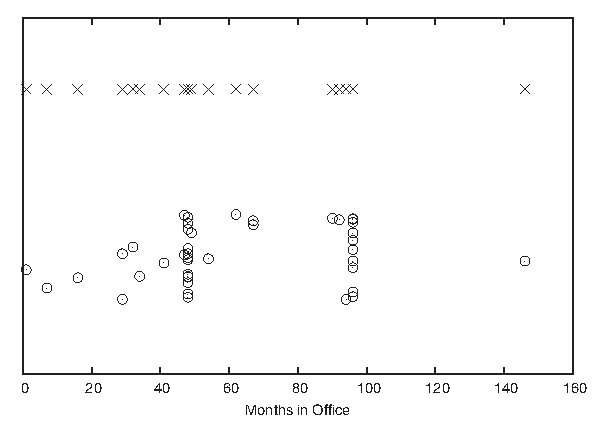
\includegraphics{img/presidents}}
  \caption{Dot and jitter plots showing the number of months U.S.\
    presidents spent in office.}
  \label{fig:presidents}
\end{figure}

What does the jitter plot tell us about the data set?  We see two
values where data points seem to cluster, indicating that these values
occur more frequently than others. Not surprisingly, they are located
at 48 and 96 months, which correspond to one and two full four-year
terms in office. What may be a little surprising, however, is the
relatively large number of points that occur \emph{outside} these
clusters.  Apparently, quite a few presidents left office at irregular
intervals!  Even in this simple example, a plot reveals both something
expected (the clusters at 48 and 96 months) and the unexpected (the
larger number of points outside those clusters).

Before moving on to our second example, let me point out a few
additional technical details regarding jitter plots.

\begin{itemize}
\item It is important that the amount of ``jitter'' be small compared
  to the distance between points. The only purpose of the random
  displacements is to ensure that no two points fall exactly on top of
  one another. We must make sure that points are not shifted
  significantly from their true location.

\item We can jitter points in either the horizontal or the vertical
  direction (or both), depending on the data set and the purpose of
  the graph. In Figure \ref{fig:presidents}, points were jittered only
  in the vertical direction, so that their horizontal position (which
  in this case corresponds to the actual data---namely, the number of
  months in office) is not altered and therefore remains exact.

\item I used open, transparent rings as symbols for the data points.
  This is no accident: among different symbols of equal size, open
  rings are most easily recognized as separate even when partially
  occluded by each other. In contrast, filled symbols tend to hide
  any substructure when they overlap, and symbols made from straight
  lines (\eg,\ boxes and crosses) can be confusing because of the large
  number of parallel lines; see the top part of Figure
  \ref{fig:presidents}.
\end{itemize}

Jittering is a good trick that can be used in many different contexts.
We will see further examples later in the book.


% ============================================================
\section{Histograms and Kernel Density Estimates}

\index{univariate analysis!histograms and kernel density estimates|(} 

Dot and jitter plots are nice because they are so simple.  However,
they are neither pretty nor very intuitive, and most importantly, they
make it hard to read off \emph{quantitative} information from the
graph. In particular, if we are dealing with larger data sets, then we
need a better type of graph, such as a histogram.

\subsection{Histograms}

\index{histograms!about|(}
 
To form a \emph{histogram}, we divide the range of values into a set
of ``bins'' and then count the number of points (sometimes called
``events'') that fall into each bin. We then plot the count of events
for each bin as a function of the position of the bin.

Once again, let's look at an example. Here is the beginning of a file
containing response times (in milliseconds) for queries against a web
server or database. In contrast to the previous example, this data
set is fairly large, containing 1,000 data points.

\begin{verbatim}
 452.42
 318.58
 144.82
 129.13
1216.45
 991.56
1476.69
 662.73
1302.85
1278.55
 627.65
1030.78
 215.23
  44.50
...
\end{verbatim}

Figure \ref{fig:serverhisto} shows a histogram of this data set. I
divided the horizontal axis into 60 bins of 50 milliseconds width and
then counted the number of events in each bin.

\begin{figure}
  \centerline{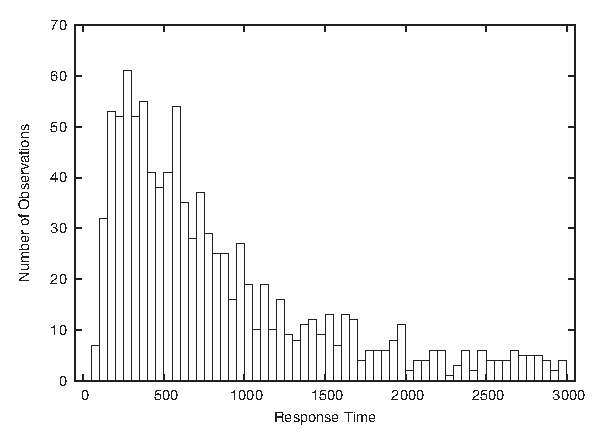
\includegraphics{img/server-data-histo}}
  \caption{A histogram of a server's response times.}
  \label{fig:serverhisto}
\end{figure}\pagebreak

What does the histogram tell us? We observe a rather sharp cutoff at a
nonzero value on the left, which means that there is a minimum
completion time below which no request can be completed. Then there is
a sharp rise to a maximum at the ``typical'' response time, and
finally there is a relatively large tail on the right, corresponding
to the smaller number of requests that take a long time to process.
This kind of shape is rather typical for a histogram of task
completion times.  If the data set had contained completion times for
students to finish their homework or for manufacturing workers to
finish a work product, then it would look qualitatively similar
except, of course, that the time scale would be different. Basically,
there is some minimum time that nobody can beat, a small group of very
fast champions, a large majority, and finally a longer or shorter tail
of ``stragglers.''

It is important to realize that a data set does not determine a
histogram uniquely. Instead, we have to fix \emph{two} parameters to
form a histogram: the bin width and the alignment of the bins.

The quality of any histogram hinges on the proper choice of bin width.
If you make the width too large, then you lose too much detailed
information about the data set. Make it too small and you will have
few or no events in most of the bins, and the shape of the distribution
does not become apparent. Unfortunately, there is no simple rule of
thumb that can predict a good bin width for a given data set;
typically you have to try out several different values for the bin
width until you obtain a satisfactory result. (As a first guess, you
can start with \emph{Scott's rule} for the bin width $w = 3.5 \sigma /
\sqrt[3]{n}$, where $\sigma$ is the standard deviation for the entire
data set and $n$ is the number of points. This rule assumes that the
data follows a Gaussian distribution;\index{Gaussian distribution (Gaussian function)!histograms} otherwise, it is likely to give
a bin width that is too wide. See the end of this chapter for more
information on the standard deviation.)

The other parameter that we need to fix (whether we realize it or
not) is the alignment of the bins on the $x$ axis. Let's say we fixed
the width of the bins at $1$.  Where do we now place the first bin? We
could put it flush left, so that its left edge is at $0$, or we could
center it at $0$. In fact, we can move all bins by half a bin width
in either direction.

Unfortunately, this seemingly insignificant (and often overlooked)
parameter can have a large influence on the appearance of the
histogram.  Consider this small data set:

\begin{verbatim}
1.4
1.7
1.8
1.9
2.1
2.2
2.3
2.6
\end{verbatim}

Figure \ref{fig:smallhisto} shows two histograms of this data set.
Both use the same bin width (namely, $1$) but have different
alignment of the bins. In the top panel, where the bin \emph{edges}
have been aligned to coincide with the whole numbers ($1, 2, 3,
\dots$), the data set appears to be flat. Yet in the bottom panel,
where the bins have been\vadjust{\pagebreak} \emph{centered} on the whole numbers, the
data set appears to have a rather strong central peak and symmetric
wings on both sides.  It should be clear that we can construct even
more pathological examples than this. In the next section we shall
introduce an alternative to histograms that avoids this particular
problem.

\begin{figure}
  \centerline{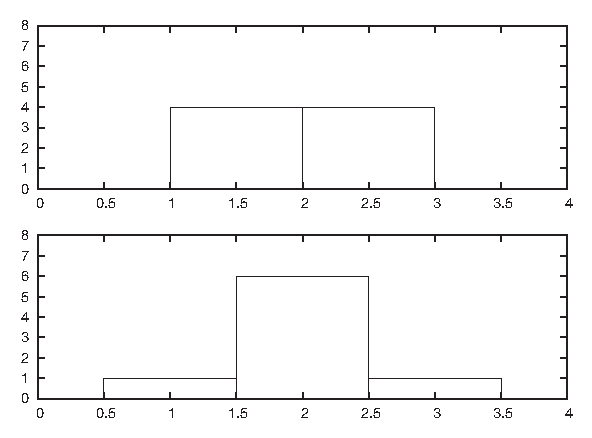
\includegraphics{img/small-histo}}
  \caption{Histograms can look quite different, depending on the
    choice of anchoring point for the first bin. The figure shows
    two histograms of the same data set, using the same bin width.
    In the top panel, the bin edges are aligned on whole numbers;
    in the bottom panel, bins are centered on whole numbers.}
  \label{fig:smallhisto}
\end{figure}

Before moving on, I'd like to point out some additional technical
details and variants of histograms.

\begin{itemize}
\item Histograms can be either normalized or unnormalized.\index{normalized histograms} \index{unnormalized histograms} In an
  \emph{unnormalized} histogram, the value plotted for each bin is the
  absolute count of events in that bin. In a \emph{normalized}
  histogram, we divide each count by the total number of points in the
  data set, so that the value for each bin becomes the fraction of
  points in that bin. If we want the percentage of points per bin
  instead, we simply multiply the fraction by $100$.

\item So far I have assumed that all bins have the same width.  We can
  relax this constraint and allow bins of differing widths---narrower
  where points are tightly clustered but wider in areas where there
  are only few points. This method can seem very appealing when the
  data set has outliers or areas with widely differing point density.
  Be warned, though, that now there is an additional source of
  ambiguity for your histogram: should you display the absolute number
  of points per bin regardless of the width of each bin; or should you
  display the density of points per bin by normalizing the point count
  per bin by the bin width?  Either method is valid, and you cannot
  assume that your audience will know which convention you are
  following.\pagebreak

\item It is customary to show histograms with rectangular boxes that
  extend from the horizontal axis, the way I have drawn Figures
  \ref{fig:serverhisto} and \ref{fig:smallhisto}.  That is perfectly
  all right and has the advantage of explicitly displaying the bin
  width as well. (Of course, the boxes should be drawn in such a way
  that they align in the same way that the actual bins align; see
  Figure \ref{fig:smallhisto}.) This works well if you are only
  displaying a histogram for a single data set. But if you want to
  compare two or more data sets, then the boxes start to get in the
  way, and you are better off drawing ``frequency polygons'': eliminate
  the boxes, and instead draw a symbol where the top of the box would
  have been.  (The horizontal position of the symbol should be at the
  center of the bin.) Then connect consecutive symbols with straight
  lines.  Now you can draw multiple data sets in the same plot
  without cluttering the graph or unnecessarily occluding points.
  % --- XXX : Reference to a freq polygon elsewhere in the text?

\item Don't assume that the defaults of your graphics program will
  generate the best representation of a histogram! I have already
  discussed why I consider frequency polygons to be almost always a
  better choice than to construct a histogram from boxes.  If you
  nevertheless choose to use boxes, it is best to avoid filling them
  (with a color or hatch pattern)---your histogram will probably look
  cleaner and be easier to read if you stick with just the box
  outlines. Finally, if you want to compare several data sets in the
  same graph, always use a frequency polygon, and stay away from
  stacked or clustered bar graphs, since these are particularly hard
  to read. (We will return to the problem of displaying composition
  problems in Chapter \ref{ch:multivariate}.)
\end{itemize}

Histograms are very common and have a nice, intuitive interpretation.
They are also easy to generate: for a moderately sized data set, it
can even be done by hand, if necessary.  That being said, histograms
have some serious problems.  The most important ones are as follows.

\begin{itemize}
\item The binning process required by all histograms loses information
  (by replacing the location of individual data points with a bin of
  finite width). If we only have a few data points, we can ill afford
  to lose any information.

\item Histograms are not unique. As we saw in Figure
  \ref{fig:smallhisto}, the appearance of a histogram can be quite
  different. (This nonuniqueness is a direct consequence of the
  information loss described in the previous item.)

\item On a more superficial level, histograms are ragged and not
  smooth.  This matters little if we just want to draw a picture of
  them, but if we want to feed them back into a computer as input for
  further calculations, then a smooth curve would be easier to handle.

\item Histograms do not handle outliers gracefully. A single outlier,
  far removed from the majority of the points, requires many empty
  cells in between or forces us to use bins that are too wide for the
  majority of points. It is the possibility of outliers that makes it
  difficult to find an acceptable bin width in an automated fashion.
\end{itemize}

Fortunately, there is an alternative to classical histograms that has
none of these problems. It is called a \emph{kernel density estimate}.

\index{histograms!about|)}

% ============================================================
\subsection{Kernel Density Estimates}

\index{kernel density estimates|(} 

Kernel density estimates (KDEs) are a relatively new technique. In
contrast to histograms, and to many other classical methods of data
analysis, they pretty much \emph{require} the calculational power of a
reasonably modern computer to be effective. They cannot be done ``by
hand'' with paper and pencil, even for rather moderately sized data
sets. (It is interesting to see how the accessibility of computational
and graphing power enables new ways to think about data!)

To form a KDE, we place a \emph{kernel}---that is, a smooth, strongly
peaked function---at the position of each data point. We then add up
the contributions from all kernels to obtain a smooth curve, which we
can evaluate at any point along the $x$ axis.

Figure \ref{fig:presidentskde} shows an example. This is yet another
representation of the data set we have seen before in Figure
\ref{fig:presidents}. The dotted boxes are a histogram of the data
set (with bin width equal to $1$), and the solid curves are two KDEs
of the same data set with different bandwidths (I'll explain this
concept in a moment). \index{bandwidth selection, KDEs} The shape of the individual kernel functions can
be seen clearly---for example, by considering the three data points
below $20$. You can also see how the final curve is composed out of
the individual kernels, in particular when you look at the points
between $30$ and $40$.

\begin{figure}
  \centerline{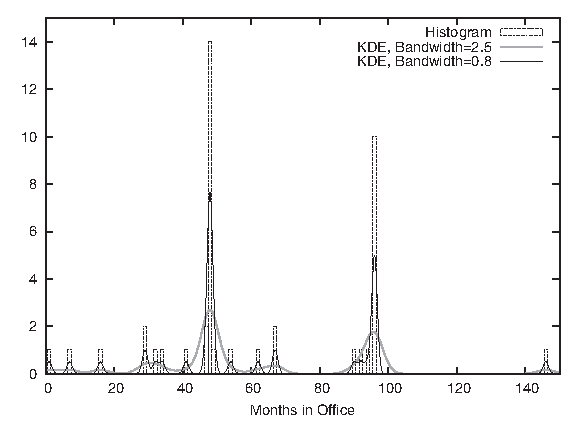
\includegraphics{img/presidents-kde}}
  \caption{Histogram and kernel density estimate of the distribution
    of the time U.S.\ presidents have spent in office.}
  \label{fig:presidentskde}
\end{figure}\pagebreak

We can use any smooth, strongly peaked function as a kernel provided
that it integrates to $1$; in other words, the area under the curve
formed by a single kernel must be $1$. (This is necessary to make sure
that the resulting KDE is properly normalized.) Some examples of
frequently used kernel functions include (see Figure
\ref{fig:kernels}):
%
\begin{align*}
K(x) & = 
\begin{cases}
  \frac{1}{2} & \text{if $\abs{x} \le 1$} \\
  0           & \text{otherwise}
\end{cases}
     & \text{box or boxcar kernel} \\
K(x) & = 
\begin{cases}
  \frac{3}{4} \paren{1-x^2} & \text{if $\abs{x} \le 1$} \\
  0                         & \text{otherwise}
\end{cases}
     & \text{Epanechnikov kernel} \\
K(x) & = \frac{1}{\sqrt{2 \pi}} \exp\paren{- \frac{1}{2} x^2}
     & \text{Gaussian kernel}
\end{align*}
%
The box kernel and the Epanechnikov kernel are zero outside a finite
range, whereas the Gaussian kernel \index{Gaussian distribution (Gaussian function)!KDEs} is nonzero everywhere but
negligibly small outside a limited domain. It turns out that the curve
resulting from the KDE does not depend strongly on the particular
choice of kernel function, so we are free to use the kernel that is
most convenient.  Because it is so easy to work with, the Gaussian
kernel is the most widely used. (See Appendix \ref{app:calculus} for
more information on the Gaussian function.)

\begin{figure}
  \centerline{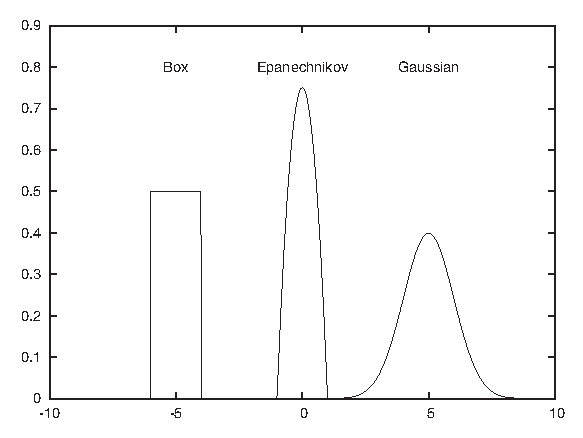
\includegraphics{img/kernels}}
  \caption{Graphs of some frequently used kernel functions.}
  \label{fig:kernels}
\end{figure}


Constructing a KDE requires to things: first, we must move the kernel
to the position of each point by shifting it appropriately.  For
example, the function $K( x - x_i )$ will have its peak at $x_i$, not
at $0$.  Second, we have to choose the kernel \emph{bandwidth},
which controls the spread of the kernel function. To make sure that
the area under the curve stays the same as we shrink the width, we
have to make the curve higher\vadjust{\pagebreak} (and lower if we increase the width).
The final expression for the shifted, rescaled kernel function of
bandwidth $h$ is:
%
\[
\frac{1}{h} K\paren{ \frac{x-x_i}{h} }
\]
%
This function has a peak at $x_i$, its width is approximately $h$, and
its height is such that the area under the curve is still $1$.  Figure
\ref{fig:gausskernel} shows some examples, using the Gaussian kernel.
Keep in mind that the area under all three curves is the same.

\begin{figure}
  \centerline{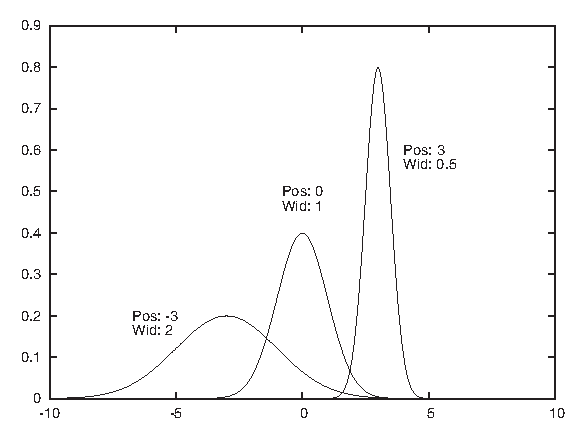
\includegraphics{img/gauss-kernel}}
  \caption{The Gaussian kernel for three different bandwidths.  The
    height of the kernel increases as the width decreases, so the
    total area under the curve remains constant.}
  \label{fig:gausskernel}
\end{figure}

Using this expression, we can now write down a formula for the KDE
with bandwidth $h$ for any data set $\braces{ x_1, x_2, \dots, x_n }$.
This formula can be evaluated for any point $x$ along the $x$ axis:
%
\[
D_h\paren{ x; \braces{ x_i } } 
  = \sum_{i=1}^n \frac{1}{h} K\paren{ \frac{x-x_i}{h} }
\]
%
All of this is straightforward and easy to implement in any computer
language. Be aware that for large data sets (those with many thousands
of points), the required number of kernel evaluations can lead to
performance issues, especially if the function $D(x)$ needs to be
evaluated for many different positions (\ie, many different values of
$x$). If this becomes a problem for you, you may want to choose a
simpler kernel function or not evaluate a kernel if the distance
$x-x_i$ is significantly greater than the bandwidth $h$.\footnote{Yet another strategy starts with the realization that
  forming a KDE amounts to a convolution of the kernel function with
  the data set. You can now take the Fourier transform of both kernel
  and data set and make use of the Fourier convolution theorem.  This
  approach is suitable for very large data sets but is outside the
  scope of our discussion.}

Now we can explain the wide gray line in Figure
\ref{fig:presidentskde}: it is a KDE with a larger bandwidth. Using
such a large bandwidth makes it impossible to resolve the individual
data points, but it does highlight entire \emph{periods} of greater or
smaller frequency. Which choice of bandwidth is right for you depends
on your purpose.

A KDE constructed as just described is similar to a classical
histogram, but it avoids two of the aforementioned problems.  Given
data set and bandwidth, a KDE is unique; a KDE is also smooth,
provided we have chosen a smooth kernel function, such as the
Gaussian.

\vspace*{-6pt}
\subsection{Optional: Optimal Bandwidth Selection}

\index{bandwidth selection, KDEs}
\index{histograms!bandwidth selection}

We still have to fix the bandwidth. This is a different \emph{kind} of
problem than the other two: it's not just a technical problem, which
could be resolved through a better method; instead, it's a fundamental
problem that relates to the data set itself.  If the data follows a
smooth distribution, then a wider bandwidth is appropriate, but if the
data follows a very wiggly distribution, then we need a smaller
bandwidth to retain all relevant detail. In other words, the optimal
bandwidth is a property of the data set and tells us something about
the nature of the data.

So how do we choose an optimal value for the bandwidth?  Intuitively,
the problem is clear: we want the bandwidth to be narrow enough to
retain all relevant detail but wide enough so that the resulting curve
is not too ``wiggly.'' This is a problem that arises in every
approximation problem: balancing the faithfulness of representation
against the simplicity of behavior. Statisticians speak of the
``bias--variance trade-off.''

To make matters concrete, we have to define a specific expression for
the error of our approximation, one that takes into account both bias
and variance. We can then choose a value for the bandwidth that
minimizes this error. For KDEs, the generally accepted measure is the
``expected mean-square error''\index{mean-square error, KDE bandwidth}  between the approximation and the true
density.  The problem is that we don't know the true density function
that we are trying to approximate, so it seems impossible to calculate
(and minimize) the error in this way. But clever methods have been
developed to make progress. These methods fall broadly into two
categories. First, we could try to find explicit expressions for
both bias and variance.  Balancing them leads to an equation that has
to be solved numerically or---if we make additional assumptions (\eg,
that the distribution is Gaussian)---can even yield explicit
expressions similar to Scott's rule (introduced earlier when talking
about histograms).  Alternatively, we could realize that the KDE is an
approximation for the probability density from which the original set
of points was chosen. We can therefore choose points from this
approximation (\ie, from the probability density represented by
the KDE) and see how well they replicate the KDE that we started with.
Now we change the bandwidth until we find that value for which the KDE
is best replicated: the result is the estimate of the ``true''
bandwidth of the data. (This latter method is known as
\emph{cross-validation}.)

Although not particularly hard, the details of both methods would lead
us too far afield, and so I will skip them here.\vadjust{\pagebreak}  If you are
interested, you will have no problem picking up the details from one
of the references at the end of this chapter.  Keep in mind, however,
that these methods find the optimal bandwidth \emph{with respect to
  the mean-square error}, which tends to overemphasize bias over variance and therefore
these methods lead to rather narrow bandwidths and KDEs that appear
too wiggly. If you are using KDEs to generate graphs for
the purpose of obtaining intuitive visualizations of point
distributions, then you might be better off with a bit of manual trial
and error combined with visual inspection.  In the end, there is no
``right'' answer, only the most suitable one for a given purpose.
Also, the most suitable to develop intuitive understanding might not
be the one that minimizes a particular mathematical quantity.

\index{univariate analysis!histograms and kernel density estimates|)} 
\index{kernel density estimates|)} 

% ============================================================
\section{The Cumulative Distribution Function}

\index{univariate analysis!cumulative distribution function|(}
\index{CDF (cumulative distribution function)|(} 
\index{cumulative distribution function (CDF)|(} 
  
The main advantage of histograms and kernel density estimates is that
they have an immediate intuitive appeal: they tell us how probable it
is to find a data point with a certain value. For example, from Figure
\ref{fig:serverhisto} it is immediately clear that values around 250
milliseconds are very likely to occur, whereas values greater than
2,000 milliseconds are quite rare.

But how rare, exactly? That is a question that is much harder to
answer by looking at the histogram in Figure \ref{fig:serverhisto}.
Besides wanting to know how much weight is in the tail, we might also
be interested to know what fraction of requests completes in the
typical band between 150 and 350 milliseconds. It's certainly the
majority of events, but if we want to know exactly how many, then we
need to sum up the contributions from all bins in that region.

The \emph{cumulative distribution function} (CDF) does just that. The CDF at
point $x$ tells us what fraction of events has occurred ``to the
left'' of $x$. In other words, the CDF is the fraction of all points
$x_i$ with $x_i \le x$.

Figure \ref{fig:serverkde} shows the same data set that we have
already encountered in Figure \ref{fig:serverhisto}, but here the data
is represented by a KDE (with bandwidth $h=30$) instead of a
histogram. In addition, the figure also includes the corresponding
CDF.  (Both KDE and CDF are normalized to $1$.)

\begin{figure}
  \centerline{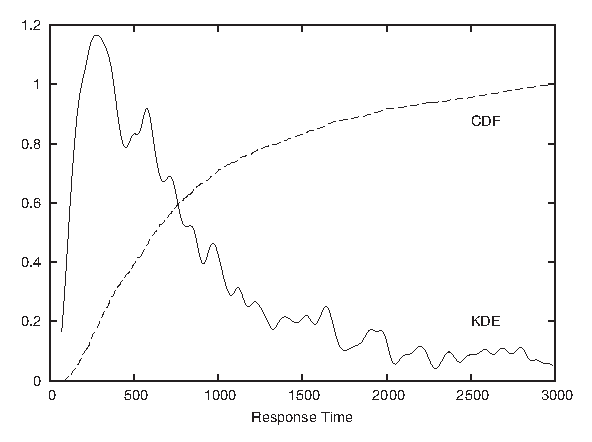
\includegraphics{img/server-data-kde}}
  \caption{Kernel density estimate and cumulative distribution
    function of the server response times shown\break in Figure
    \ref{fig:serverhisto}.}\label{fig:serverkde}
\end{figure}

We can read off several interesting observations directly from the
plot of the CDF. For instance, we can see that at $t=\text{1,500}$
(which certainly puts us into the tail of the distribution) the CDF is
still smaller than $0.85$; this means that fully 15 percent of all
requests take longer than 1,500 milliseconds. In contrast, less than a
third of all requests are completed in the ``typical'' range of
150--500 milliseconds.  (How do we know this? The CDF for $t=150$ is
about $0.05$ and is close to $0.40$ for $t=500$. In other words, about
40 percent of all requests are completed in less than $500$
milliseconds; of these, 5 percent are completed in less than $150$
milliseconds.  Hence about 35 percent of all requests have response
times of between $150$ and $500$ milliseconds.)

It is worth pausing to contemplate these findings, because they
demonstrate how misleading a histogram (or KDE) can be despite (or
because of) their intuitive appeal! Judging from the histogram or KDE
alone, it seems quite reasonable to assume that ``most'' of the events
occur within the major peak near $t=300$ and that the tail for $t >
\text{1,500}$ contributes relatively little. Yet the CDF tells us
clearly that this is not so. (The problem is that the eye is much
better at judging distances than areas, and we are therefore misled by
the large values of the histogram near its peak and fail to see that
nevertheless the area beneath the peak is not that large compared to
the total area under the curve.)

CDFs are probably the least well-known and most underappreciated tool
in basic graphical analysis. They have less immediate intuitive appeal
than histograms or KDEs, but they allow us to make the kind of
quantitative statement that is very often required but is
difficult (if not impossible) to obtain from a histogram.

Cumulative distribution functions have a number of important
properties that follow directly from how they are calculated.

\begin{itemize}
\item Because the value of the CDF at position $x$ is the fraction of
  points to the left of $x$, a CDF is always monotonically increasing
  with $x$.

\item CDFs are less wiggly than a histogram (or KDE) but contain the
  same information in a representation that is inherently less noisy.

\item Because CDFs do not involve any binning, they do not lose
  information and are therefore a more faithful representation of the
  data than a histogram.

\item All CDFs approach $0$ as $x$ goes to negative infinity. CDFs
  are usually normalized so that they approach $1$ (or 100 percent) as
  $x$ goes to positive infinity.

\item A CDF is unique for a given data set.
\end{itemize}

If you are mathematically inclined, you have probably already realized
that the CDF is (an approximation to) the antiderivative of the
histogram and that the histogram is the derivative of the CDF:\vspace*{-3pt}
%
\begin{gather*}
\operatorname{cdf}(x) 
  \approx \int_{-\infty}^{x} \lms{t} \operatorname{histo}(t) \\
\operatorname{histo}(x) 
  \approx \Diff{x} \operatorname{cdf}(x)
\end{gather*}
%
Cumulative distribution functions have several uses. First, and most
importantly, they enable us to answer questions such as those posed
earlier in this section: what fraction of points falls between any two
values? The answer can simply be read off from the graph. Second, CDFs
also help us understand how imbalanced a distribution is---in other
words, what fraction of the overall weight is carried by the tails.

Cumulative distribution functions also prove useful when we want to
compare two distributions. It is notoriously difficult to compare two
bell-shaped curves in a histogram against each other. Comparing the
corresponding CDFs is usually much more conclusive.

One last remark, before leaving this section: in the literature, you
may find the term \emph{quantile plot}.\index{quantile plots}  A quantile plot is just the
plot of a CDF in which the $x$ and $y$ axes have been switched.
Figure \ref{fig:serverquantile} shows an example using once again the
server response time data set. Plotted this way, we can easily answer
questions such as, ``What response time corresponds to the 10th
percentile of response times?''  But the information contained in this
graph is of course exactly the same as in a graph of the CDF.

\begin{figure}
  \centerline{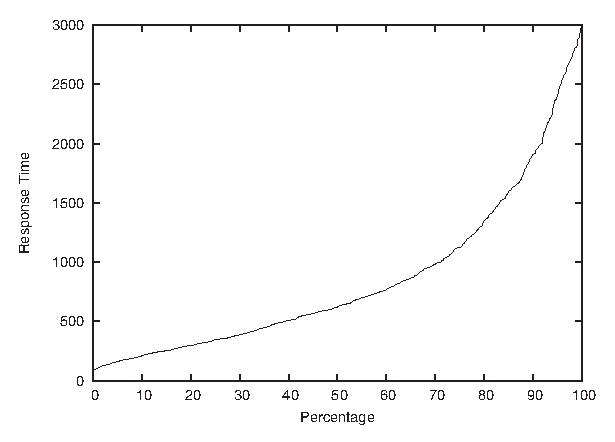
\includegraphics{img/serverquantile}}
  \caption{Quantile plot of the server data. A quantile plot is a
    graph of the CDF with the $x$ and $y$ axes interchanged. Compare
    to Figure \ref{fig:serverkde}.}
  \label{fig:serverquantile}
\end{figure}

\vspace*{-6pt}
\subsection{Optional: Comparing Distributions with Probability Plots and QQ Plots}

\index{probability plots, comparing with distributions|(}
\index{QQ plots!comparing with distributions|(}

Occasionally you might want to confirm that a given set of points 
is distributed according to some specific, known distribution. For
example, you have a data set and would like to determine whether it
can be described well by a Gaussian (or some other) distribution.

% --- XXX : not yet explained: density function. Does it matter?
You could compare a histogram or KDE of the data set directly against
the theoretical density function, but it is notoriously difficult to
compare distributions that way---especially out in the tails.  A
better idea would be to compare the cumulative distribution functions,
which are easier to handle because they are less wiggly and are always
monotonically increasing. But this is still not easy. Also keep in
mind that most probability distributions depend on location and scale
parameters (such as mean and variance), which you would have to
estimate \emph{before} being able to make a meaningful comparison.
Isn't there a way to compare a set of points directly against a
theoretical distribution and, in the process, read off the estimates
for all the parameters required?

As it turns out, there is. The method is technically easy to do, but
the underlying logic is a bit convoluted and tends to trip up even
experienced practitioners.


\begin{figure}
  \centerline{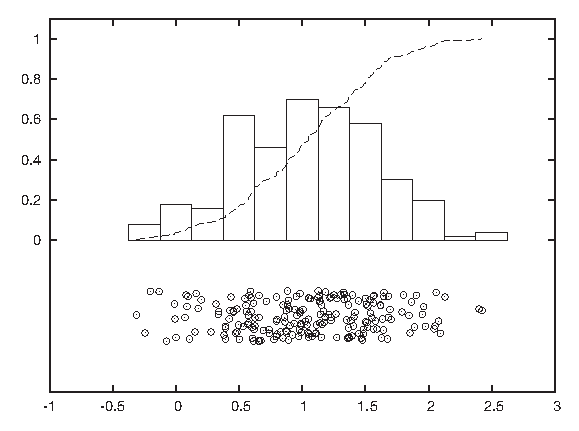
\includegraphics{img/happyqq1}}
  \caption{Jitter plot, histogram, and cumulative distribution function
    for a Gaussian data set.}
  \label{fig:happyqq1}
\end{figure}

Here is how it works. Consider a set of points $\braces{x_i}$ that we
suspect are distributed according to the Gaussian distribution. In 
other words, we expect the cumulative distribution function of the
set\vadjust{\pagebreak} of points, $y_i = \operatorname{cdf}(x_i)$, to be the Gaussian 
cumulative distribution function $\Phi\paren{ (x-\mu)/\sigma }$
with mean $\mu$ and standard deviation $\sigma$:
%
\[
y_i = \Phi\paren{ \frac{x_i-\mu}{\sigma } } 
  \quad \text{only if data is Gaussian}
\]
%
Here, $y_i$ is the value of the cumulative distribution function 
corresponding to the data point $x_i$; in other words, $y_i$ is
the \emph{quantile} of the point $x_i$.

Now comes the trick. We apply the \emph{inverse} of the Gaussian
distribution function to both sides of the equation:
%
\[
\Phi^{-1}(y_i) = \frac{x_i-\mu}{\sigma }
\]
%
With a little bit of algebra, this becomes
%
\[
x_i = \mu + \sigma \Phi^{-1}(y_i)
\]
%
In other words, if we plot the values in the data set as a function of
$\Phi^{-1}(y_i)$, then they should fall onto a straight line with
slope $\sigma$ and zero intercept $\mu$. If, on the other hand, the
points do not fall onto a straight line after applying the inverse
transform, then we can conclude that the data is not distributed
according to a Gaussian distribution.

\begin{figure}
  \centerline{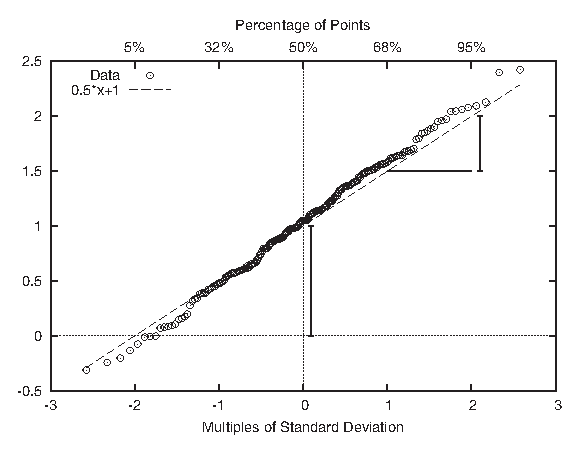
\includegraphics{img/happyqq2}}
  \caption{Probability plot for the data set shown in Figure 
    \ref{fig:happyqq1}.}
  \label{fig:happyqq2}
\end{figure}

The resulting plot is known as a \emph{probability plot}. Because it
is easy to spot deviation from a straight line, a probability plot
provides a relatively sensitive test to determine whether a set of
points behaves according to the Gaussian distribution. As an added
benefit, we can read off estimates for the mean and the standard
deviation directly from the graph: $\mu$ is the intercept of the curve
with the $y$ axis, and $\sigma$ is given by the slope of the curve.
(Figure \ref{fig:happyqq2} shows the probability plot for the Gaussian
data set displayed in Figure \ref{fig:happyqq1}.)

One important question concerns the \emph{units} that we plot along
the axes. For the vertical axis the case is clear: we use whatever
units the original data was measured in. But what about the horizontal
axis? We plot the data as a function of $\Phi^{-1}(y_i)$, which is the
inverse Gaussian distribution function, applied to the percentile
$y_i$ for each point $x_i$. We can therefore choose between two
different ways to dissect the horizontal axis: either using the
percentiles $y_i$ directly (in which case the tick marks will not be
distributed uniformly), or dividing the horizontal axis uniformly. In
the latter case we are using \emph{the width of the standard Gaussian
  distribution} as a unit. You can convince yourself that this is
really true by realizing that $\Phi^{-1}(y)$ is the inverse of the
Gaussian distribution function $\Phi(x)$. Now ask yourself: what units
is $x$ measured in? We use the same units for the horizontal axis of a
Gaussian probability plot.  These units are sometimes called
\emph{probits}. (Figure \ref{fig:happyqq2} shows both sets of units.)
Beware of confused and confusing explanations of this point elsewhere
in the literature.

There is one more technical detail that we need to discuss: to produce
a probability plot, we need not only the data itself, but for each
point $x_i$ we also need its quantile $y_i$ (we will discuss
quantiles and percentiles in more detail later in this chapter). The
simplest way to obtain the quantiles, given the data, is as follows:

\begin{enumerate}
\item Sort the data points in ascending order.
\item Assign to each data point its rank (basically, its line number
  in the sorted file), starting at $1$ (not at $0$).
\item The quantile $y_i$ now is the rank divided by $n+1$, where
  $n$ is the number of data points.
\end{enumerate}

This prescription guarantees that each data point is assigned a
quantile that is strictly greater than $0$ and strictly less than $1$.
This is important because $\Phi^{-1}(x)$ is defined only for $0 < x <
1$. This prescription is easy to understand and easy to remember, but
you may find other, slightly more complicated prescriptions elsewhere.
For all practical purposes, the differences are going to be small.

Finally, let's look at an example where the data is clearly \emph{not}
Gaussian. Figure \ref{fig:serverdataqq} shows the server data from
Figure \ref{fig:serverhisto} plotted in a probability plot.  The
points don't fall on a straight line at all---which is no surprise
since we already knew from Figure \ref{fig:serverhisto} that the data
is not Gaussian.  But for cases that are less clear-cut, the
probability plot can be a helpful tool for detecting deviations from
Gaussian behavior.
% Long tails: data in tails ``steeper'' than straight line
% Short tails: data in tails ``flatter'' than straight line

\begin{figure}
  \centerline{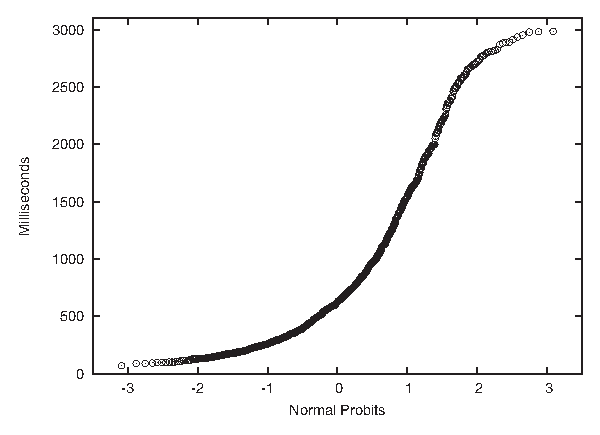
\includegraphics{img/serverdataqq}}
  \caption{A probability plot of the server response times from Figure
    \ref{fig:serverhisto}. The data does not follow a Gaussian
    distribution and thus the points do \emph{not} fall on a straight
    line.}
  \label{fig:serverdataqq}
\end{figure}

A few additional comments are in order here.

\begin{itemize}
\item Nothing in the previous discussion requires that the
  distribution be Gaussian! You can use almost any other commonly used
  distribution function (and its inverse) to generate the respective
  probability plots. In particular, many of the commonly used\vadjust{\vfill\pagebreak}
  probability distributions depend on location and scale parameters in
  exactly the same way as the Gaussian distribution, so all the
  arguments discussed earlier go through as before.
\item So far, I have always assumed that we want to compare an
  \emph{empirical} data set against a \emph{theoretical} distribution.
  But there may also be situations where we want to compare two
  empirical data sets against each other---for example, to find out
  whether they were drawn from the same family of distributions
  (without having to specify the family explicitly). The process is
  easiest to understand when both data sets we want to compare contain
  the same number of points. You sort both sets and then align the
  points from both data sets that have the same rank (once sorted).
  Now plot the resulting pairs of points in a regular scatter plot
  (see Chapter \ref{ch:bivariate}); the resulting graph is known as a
  \emph{QQ plot}. (If the two data sets do not contain the same number
  of points, you will have to interpolate or truncate them so that
  they do.)
\end{itemize}

Probability plots are a relatively advanced, specialized technique,
and you should evaluate whether you really need them. Their purpose is
to determine whether a given data set stems from a specific, known
distribution. Occasionally, this is of interest in itself; in other
situations subsequent analysis depends on proper identification of the
underlying model. For example, many statistical techniques assume that
the errors or residuals are Gaussian and are not applicable if this
condition is violated.  Probability plots are a convenient technique
for testing this assumption.
\index{univariate analysis!cumulative distribution function|)}
\index{CDF (cumulative distribution function)|)} 
\index{cumulative distribution function (CDF)|)} 
\index{probability plots, comparing with distributions|)}
\index{QQ plots!comparing with distributions|)}\vfill\pagebreak

% ============================================================
\section{Rank-Order Plots and Lift Charts}

\index{univariate analysis!rank-order plots and lift charts|(}
\index{rank-order plots|(}
\index{lift charts|(}

There is a technique related to histograms and CDFs that is worth
knowing about. Consider the following scenario. A company that is
selling textbooks and other curriculum materials is planning an email
marketing campaign to reach out to its existing customers.  For this
campaign, the company wants to use personalized email messages that
are tailored to the job title of each recipient (so that teachers will
receive a different email than their principals).  The problem is the
customer database contains about 250,000 individual customer records
with over 16,000 different job titles among them! Now what?

The trick is to sort the job titles by the number of individual
customer records corresponding to each job title. The first few
records are shown in Table \ref{tbl:jobtitles}. The four columns give
the job title, the number of customers for that job title, the
fraction of all customers having that job title, and finally the
cumulative fraction of customers. For the last column, we sum up the
number of customers for the current and all previously seen job
titles, then divide by the total number of customer records. This is
the equivalent of the CDF we discussed earlier.

We can see immediately that fully two thirds of all customers account
for only 10 different job titles. Using just the top 30 job titles
gives us 75 percent coverage of customer records. That's much more
manageable than the 16,000 job titles we started with!

\begin{table}
\newlength{\unicola}
\newlength{\unicolb}
\newlength{\unicolc}
\settowidth{\unicola}{Number ofX}
\settowidth{\unicolb}{Fraction ofX}
\settowidth{\unicolc}{Cumulative}
\tbl{The first 30 job titles and their relative frequencies.\label{tbl:jobtitles}}{%
\begin{tabular}{lrrr}
\toprule
   & \textbf{Number of}
   & \textbf{Fraction of}
  & \textbf{Cumulative} \\
\textbf{Title} &  \textbf{customers} & \textbf{customers} & \textbf{fraction}\\
\colrule
Teacher \rule{0mm}{4mm}  & 66,470  &  0.34047   &   0.340 \\ 
Principal                & 22,958  &  0.11759   &   0.458 \\
Superintendent           & 12,521  &  0.06413   &   0.522 \\
Director                 & 12,202  &  0.06250   &   0.584 \\
Secretary                &  4,427  &  0.02267   &   0.607 \\
Coordinator              &  3,201  &  0.01639   &   0.623 \\
Vice Principal           &  2,771  &  0.01419   &   0.637 \\
Program Director         &  1,926  &  0.00986   &   0.647 \\
Program Coordinator      &  1,718  &  0.00880   &   0.656 \\
Student                  &  1,596  &  0.00817   &   0.664 \\
Consultant               &  1,440  &  0.00737   &   0.672 \\
Administrator            &  1,169  &  0.00598   &   0.678 \\
President                &  1,114  &  0.00570   &   0.683 \\
Program Manager          &  1,063  &  0.00544   &   0.689 \\
Supervisor               &  1,009  &  0.00516   &   0.694 \\
Professor                &    961  &  0.00492   &   0.699 \\
Librarian                &    940  &  0.00481   &   0.704 \\
Project Coordinator      &    880  &  0.00450   &   0.708 \\
Project Director         &    866  &  0.00443   &   0.713 \\
Office Manager           &    839  &  0.00429   &   0.717 \\
Assistant Director       &    773  &  0.00395   &   0.721 \\
Administrative Assistant &    724  &  0.00370   &   0.725 \\
Bookkeeper               &    697  &  0.00357   &   0.728 \\
Intern                   &    693  &  0.00354   &   0.732 \\
Program Supervisor       &    602  &  0.00308   &   0.735 \\
Lead Teacher             &    587  &  0.00300   &   0.738 \\
Instructor               &    580  &  0.00297   &   0.741 \\
Head Teacher             &    572  &  0.00292   &   0.744 \\
Program Assistant        &    572  &  0.00292   &   0.747 \\
Assistant Teacher        &    546  &  0.00279   &   0.749\\
\botrule
\end{tabular}}
\end{table}

Let's step back for a moment to understand how this example is
different from those we have seen previously. What is important to
notice here is that \emph{the independent variable has no intrinsic
  ordering}. What does this mean?

For the web-server example, we counted the number of events for each
response time; hence the count of events per bin was the dependent
variable, and it was determined by the independent variable---namely,
the response time. In that case, the independent variable had an
inherent ordering: 100 milliseconds are always less than 400
milliseconds (and so on). But in the case of counting customer records
that match a certain job title, the independent variable (the job
title) has no corresponding ordering relation. It may appear otherwise
since we can sort the job titles alphabetically, but realize that this
ordering is entirely arbitrary! There is nothing ``fundamental'' about
it. If we choose a different font encoding or locale, the order will
change.  Contrast this with the ordering relationship on
numbers---there are no two ways about it: 1 is always less than 2.

In cases like this, where the independent variable does not have an
intrinsic ordering, it is often a good idea to sort entries by the
\emph{dependent} variable. That's what we did in the example: rather
than defining some (arbitrary) sort order on the job titles, we sorted
by the number of records (\ie, by the dependent variable). Once the
records have been sorted in this way, we can form a histogram and a
CDF as before.

This trick of sorting by the dependent variable is useful whenever the
independent variable does not have a meaningful ordering relation; it
is not limited to situations where we count events per bin. Figures
\ref{fig:sales} and \ref{fig:pareto} show two typical examples.
\begin{figure}
  \centerline{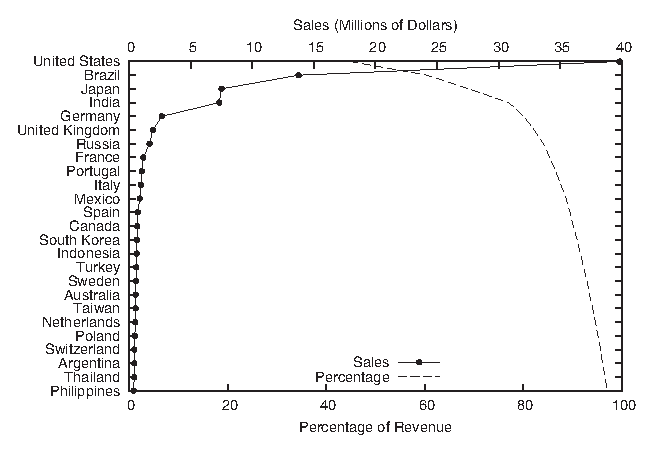
\includegraphics{img/sales}}
  \caption{A rank-order plot of sales per country. The independent
    variable has been plotted along the \emph{vertical} axis to make
    the text labels easier to read.}
  \label{fig:sales}
\end{figure}

Figure \ref{fig:sales} shows the sales by a certain company to
different countries. Not only the sales to each country but also the
cumulative sales are shown, which allows us to assess the importance
of the remaining ``tail'' of the distribution of sales.

In this example, I chose to plot the independent variable along the
vertical axis. This is often a good idea when the values are strings,
since they are easier to read this way. (If you plot them along the
horizontal axis, it is often necessary to rotate the strings by 90
degrees to make them fit, which makes hard to read.)

\begin{figure}
  \centerline{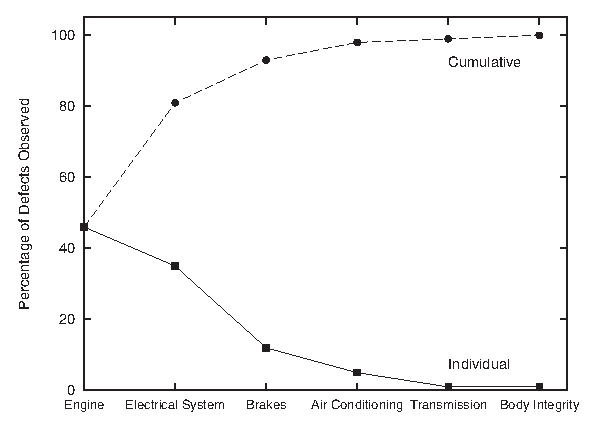
\includegraphics{img/pareto}}
  \caption{The Pareto chart is another example of a rank-order plot.}
  \label{fig:pareto}
\end{figure}

Figure \ref{fig:pareto} displays what in quality engineering is known
as a \emph{Pareto chart}. \index{Pareto charts} In quality engineering and
process improvement,\vadjust{\pagebreak} the goal is to reduce the number of defects in
a certain product or process. You collect all known causes of defects and
observe how often each one occurs. The results can be summarized
conveniently in a chart like the one in Figure \ref{fig:pareto}. Note
that the causes of defects are sorted by their frequency of
occurrence. From this chart we can see immediately that problems with
the engine and the electrical system are much more common than
problems\vadjust{\pagebreak} with the air conditioning, the brakes, or the transmission.
In fact, by looking at the cumulative error curve, we can tell that
fixing just the first two problem areas would reduce the overall
defect rate by 80 percent.

Two more bits of terminology: the term ``Pareto chart'' is not used
widely outside the specific engineering disciplines mentioned in the
previous paragraph. I personally prefer the expression
\emph{rank-order chart} for any plot generated by first sorting all
entries by the dependent variable (\ie, by the \emph{rank} of the
entry). The cumulative distribution curve is occasionally referred to
as a \emph{lift curve}, \index{lift curves} because it tells us how much ``lift'' we get
from each entry or range of entries.
      
\index{univariate analysis!rank-order plots and lift charts|)}
\index{rank-order plots|)}
\index{lift charts|)}

%============================================================
\section{Only When Appropriate: Summary Statistics and Box Plots}

\index{univariate analysis!summary statistics and box plots|(}
   
You may have noticed that so far I have not spoken at all about such
simple topics as mean and median, standard deviation, and 
percentiles.\index{mean!about}\index{median}\index{standard deviation}\index{percentiles} 
That is quite intentional. These \emph{summary statistics} apply only
under certain assumptions and are misleading, if not downright wrong,
if those assumptions are not fulfilled. I know that these quantities
are easy to understand and easy to calculate, but if there is one
message I would like you to take away from this book it is this: the
fact that something is convenient and popular is no reason to follow
suit. For any method that you want to use, make sure you understand
the underlying assumptions and \emph{always} check that they are
fulfilled for the specific application you have in mind!

Mean, median, and related summary statistics apply only to
distributions that have a single, central peak---that is, to
\emph{unimodal} distributions. If this basic assumption is not
fulfilled, then conclusions based on simple summary statistics will be
wrong. Even worse, nothing will tip you off that they are wrong: the
numbers will look quite reasonable. (We will see an example of this
problem shortly.)

\subsection{Summary Statistics}

\index{summary statistics|(}

If a distribution has only a single peak, then it makes sense to ask
about the properties of that peak: where is it located, and what is
its width? We may also want to know whether the distribution is
symmetric and whether any outliers are present.

Mean and standard deviation are two popular measures for location and
spread. The \emph{mean} or average is both familiar and intuitive:
%
\[
m = \frac{1}{n} \sum_i x_i
\]
%
The standard deviation measures how far points spread ``on average''
from the mean: we take all the differences between each individual
point and the mean, and then calculate the average of all these
differences. Because data points can either overshoot or undershoot
the mean and we don't\vadjust{\pagebreak} want the positive and negative deviations to
cancel each other, we sum the \emph{square} of the individual
deviations and then take the mean of the square deviations.  (The
second equation is very useful in practice and can be found from the
first after plugging in the definition of the mean.)
%
\begin{align*}
s^2 & = \frac{1}{n} \sum_i \paren{ x_i - m }^2 \\
    & = \frac{1}{n} \sum_i x_i^2 - m^2
\end{align*}
%
The quantity $s^2$ calculated in this way is known as the
\emph{variance} and is the more important quantity from a theoretical
point of view. But as a measure of the spread of a distribution, we are
better off using its square root, which is known as the \emph{standard
  deviation}. Why take the square root?  Because then both measure for
the location, and the measure for the spread will have the same units,
which are also the units of the actual data. (If our data set consists
of the prices for a basket of goods, then the variance would be given
in ``square dollars,'' whereas the standard deviation would be given
in dollars.)

For many (but certainly not all!) data sets arising in practice, one
can expect about two thirds of all data points to fall within the
interval $[m-s, m+s]$ and 99 percent of all points to fall within the
wider interval $[m-3s, m+3s]$.

Mean and standard deviation are easy to calculate, and have certain
nice mathematical properties---provided the data is symmetric and does
not contain crazy outliers. Unfortunately, many data sets violate at
least one of these assumptions. Here is an example for the kind of
trouble that one may encounter. Assume we have 10 items costing \$1
each, and one item costing \$20. The mean item price comes out to be
\$2.73, even though no item has a price anywhere near this value. The
standard deviation is even~worse: it comes out to \$5.46, implying
that most items have a price between $\text{\$2.73}-\text{\$5.46}$ and
$\text{\$2.73}+\text{\$5.46}$. The ``expected range'' now includes
negative prices---an obviously absurd result. Note that the data set
itself is not particularly pathological: going to the grocery store
and picking up a handful of candy bars and a bottle of wine will do it
(pretty good wine, to be sure, but nothing outrageous).

A different set of summary statistics that is both more flexible and
more robust is based on the concepts of \emph{median}\index{median} and
\emph{quantiles}\index{quantiles} or \emph{percentiles}.\index{percentiles} The median is conventionally
defined as the value from a data set such that half of all points in
the data set are smaller and the other half greater that that value.
Percentiles are the generalization of this concept to other fractions
(the 10th percentile is the value such that 10 percent of all points
in the data set are smaller than it, and so on).  Quantiles are
similar to percentiles, only that they are taken with respect to the
fraction of points, not the percentage of points (in other words, the
10th percentile equals the 0.1 quantile).

Simple as it is, the percentile concept is nevertheless ambiguous, and
so we need to work a little harder to make it really concrete. As an
example of the problems that occur, consider the data set $\braces{ 1,
  2, 3 }$. What is the median?\vadjust{\pagebreak} It is not possible to break this data
set into two equal parts each containing exactly half the points. The
problem becomes even more uncomfortable when we are dealing with
arbitrary percentile values (rather than the median only).

The Internet standard laid down in RFC 2330 (``Framework for IP
Performance Metrics'') gives a definition of percentiles in terms of
the CDF, which is unambiguous and practical, as follows.  The $p$th
percentile is the smallest value $x$, such that the cumulative
distribution function of $x$ is greater or equal $p/100$.
\[
\text{$p$th percentile: smallest $x$ for which }
\operatorname{cdf}(x) \ge p/100
\]
This definition assumes that the CDF is normalized to 1,
not to 100. If it were normalized to 100, the condition would be
$\operatorname{cdf}(x) \ge p$.

With this definition, the median (\ie, the 50th percentile) of the
data set $\braces{1,2,3}$ is $2$ because the $\operatorname{cdf}(1) =
0.33\dots$, $\operatorname{cdf}(2) = 0.66\dots$, and
$\operatorname{cdf}(3) = 1.0$.  The median of the data set
$\braces{1,2}$ would be $1$ because now $\operatorname{cdf}(1) = 0.5$,
and $\operatorname{cdf}(2) = 1.0$.

The median is a measure for the location of the distribution, and we
can use percentiles to construct a measure for the width of the
distribution. Probably the most frequently used quantity for this
purpose is the \emph{inter-quartile range} (IQR), which is the
distance between the 75th percentile and 25th percentile.

When should you favor median and percentile over mean and standard
deviation? Whenever you suspect that your distribution is not
symmetric or has important outliers.

If a distribution is symmetric and well behaved, then mean and median
will be quite close together, and there is little difference in using
either. Once the distribution becomes skewed, however, the basic
assumption that underlies the mean as a measure for the location of
the distribution is no longer fulfilled, and so you are better off
using the median. (This is why the average wage is usually given in
official publications as the median family income, not the mean; the
latter would be significantly distorted by the few households with
extremely high incomes.) Furthermore, the moment you have outliers,
the assumptions behind the standard deviation as a measure of the
width of the distribution are violated; in this case you should favor
the IQR (recall our shopping basket example earlier).

If median and percentiles are so great, then why don't we always use
them?  A large part of the preference for mean and variance is
historical. In the days before readily available computing power,
percentiles were simply not practical to calculate. Keep in mind that
finding percentiles requires to \emph{sort} the data set whereas to
find the mean requires only to add up all elements in any order. The
latter is an $\mathcal{O}(n)$ process, but the former is an
$\mathcal{O}(n^2)$ process, since humans---being nonrecursive---cannot
be taught Quicksort and therefore need to resort to much less
efficient sorting algorithms. A second reason is that it is much harder
to prove rigorous theorems for percentiles, whereas mean and variance
are mathematically very well behaved and easy to work with.

\index{summary statistics|)}

\subsection{Box-and-Whisker Plots}

\index{box-and-whisker plots!about|(}

There is an interesting graphical way to represent these quantities,
together with information about potential outliers, known as a
\emph{box-and-whisker plot}, or \emph{box plot} for short. Figure
\ref{fig:glassboxplot} illustrates all components of a box plot. A box
plot consists of:

\begin{itemize}
\item A \emph{marker} or symbol for the median as an indicator of the
  \emph{location} of the distribution

\item A \emph{box}, spanning the inter-quartile range, as a measure of
  the \emph{width} of the distribution

\item A set of \emph{whiskers}, extending from the central box to the
  upper and lower adjacent values, as an indicator of the \emph{tails}
  of the distribution (where ``adjacent value'' is defined in the next
  paragraph)

\item Individual \emph{symbols} for all values outside the range of
  adjacent values, as a representation for \emph{outliers}
\end{itemize}

You can see that a box plot combines a lot of information in a single
graph. We have encountered almost all of these concepts before, with
the exception of upper and lower \emph{adjacent values}. While the
inter-quartile range is a measure for the width of the central
``bulk'' of the distribution, the adjacent values are one possible way
to express how far its tails reach.  The upper adjacent value is the
largest value in the data set that is less than twice the
inter-quartile range greater than the median. In other words: extend
the whisker upward from the median to twice the length of the central
box. Now trim the whisker down to the largest value that actually
occurs in the data set; this value is the upper adjacent value. (A
similar construction holds for the lower adjacent value.)

You may wonder about the reason for this peculiar construction. Why
not simply extend the whiskers to, say, the 5th and 95th percentile
and be done with it? The problem with this approach is that it does
not allow us to recognize true outliers! Outliers are data points that
are, \emph{when compared to the width of the distribution}, unusually
far from the center. Such values may or may not be present.  The top
and bottom 5 percent, on the other hand, are always present even for
very compact distributions. To recognize outliers, we therefore cannot
simply look at the most extreme values, instead we must \emph{compare
  their distance from the center to the overall width of the
  distribution}.  That is what box-and-whisker plots, as described in
the previous paragraph, do.

The logic behind the preceding argument is extremely important (not
only in this application but more generally), so I shall reiterate the
steps: \emph{first} we calculated a measure for the width of the
distribution, \emph{then} we used this width to identify outliers as
those points that are far from the center, where (and this is the
crucial step) ``far'' is measured in units of the width of the
distribution. We neither impose an arbitrary distance from the
outside, nor do we simply label the most extreme $x$ percent of the
distribution as outliers---instead, we determine the width of the
distribution (as the range into which points ``typically'' fall) and
then use it to identify outliers as those points that deviate from
this range.  The important insight here is that the distribution
itself determines a typical \emph{scale}, which provides a natural
unit in which\vadjust{\pagebreak} to measure other properties of the distribution. This
idea of using some typical property of the system to describe other
parts of the system will come up again later (see Chapter
\ref{ch:scaling}).

Box plots combine many different measures of a distribution into a
single, compact graph. A box plot allows us to see whether the
distribution is symmetric or not and how the weight is distributed
between the central peak and the tails. Finally, outliers (if present)
are not dropped but shown explicitly.

Box plots are best when used to compare several distributions against
one another---for a single distribution, the overhead of preparing
and managing a graph (compared to just quoting the numbers) may often 
not appear justified. Here is an example that compares different data
sets against each other.

Let's say we have a data set containing the index of refraction of 121
samples of glass.\footnote{The raw data can be found in the ``Glass
  Identification Data Set'' on the UCI Machine Learning Repository at
  \url{http://archive.ics.uci.edu/ml/}.} The data
set is broken down by the type of glass: 70 samples of window glass,
29 from headlamps, 13 from containers of various kinds, and 9 from
tableware. Figures \ref{fig:glasskde} and \ref{fig:glassboxplot} are
two representations of the same data, the former as a kernel density
estimate and the latter as a box plot.

The box plot emphasizes the overall structure of the data sets and
makes it easy to compare the data sets based on their location and
width. At the same time, it also loses much information. The KDE gives
a more detailed view of the data---in particular showing the
occurrence of multiple peaks in the distribution functions---but makes
it more difficult to quickly sort and classify the data sets.
Depending on your needs, one or the other technique may be preferable
at any given time.

Here are some additional notes on box plots.

\begin{itemize}
\item The specific way of drawing a box plot that I described here is
  especially useful but is far from universal. In particular, the
  specific definition of the adjacent values is often not properly
  understood. Whenever you find yourself looking at a box plot, always
  ask what exactly is shown, and whenever you prepare one, make sure
  to include an explanation.

\item The box plot described here can be modified and enhanced.  For
  example, the width of~the central box (\ie, the direction orthogonal
  to the whiskers) can be used to indicate the size of the underlying
  data set: the more points are included, the wider the box. Another
  possibility is to abandon the rectangular shape of the box
  altogether and to use the local width of the box to display the
  density of points at each location---\break which brings us almost full
  circle to KDEs.
\end{itemize}

\index{univariate analysis!summary statistics and box plots|)}
\index{box-and-whisker plots!about|)}


\begin{figure}
  \centerline{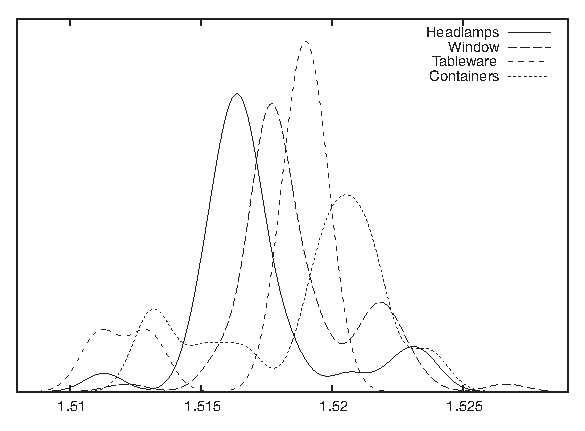
\includegraphics{img/glass-kde}}
  \caption{Comparing data sets using KDEs: refractive index of different
    types of glass. (Compare Figure \ref{fig:glassboxplot}.)}
  \label{fig:glasskde}\vspace*{-6pt}
\end{figure} 

% ============================================================
\section{Workshop: NumPy}

\index{NumPy|(}
\index{software!NumPy|(}
 
The NumPy module provides efficient and convenient handling of large
numerical arrays in Python.  It is the successor to both the earlier
Numeric and the alternative numarray modules. (See the Appendix
\ref{app:tools} for more on the history of scientific computing with
Python.) The NumPy module is used by many other libraries and projects
and in this sense is a ``base'' technology.

\begin{figure}
\vspace*{-6pt}
  \centerline{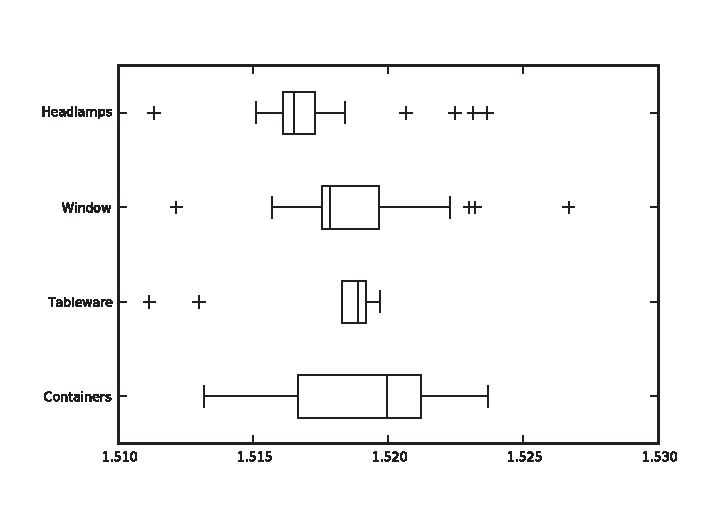
\includegraphics{img/glass-boxplot}}\vspace*{-6pt}
  \caption{Comparing data sets using box plots: refractive index of 
    different types of glass. (Compare Figure \ref{fig:glasskde}.)}
  \label{fig:glassboxplot}\vspace*{-6pt}
\end{figure}

Let's look at some quick examples before delving a bit deeper into
technical details.

\vspace*{-9pt}
\subsection{NumPy in Action}

NumPy objects are of type \texttt{ndarray}.  There are different ways
of creating them. We can create an \texttt{ndarray} by:

\begin{itemize}
\item Converting a Python list
\item Using a factory function that returns a populated vector
\item Reading data from a file directly into a NumPy object
\end{itemize}

The listing that follows shows five different ways to create NumPy
objects.  First we create one by converting a Python list. Then we
show two different factory routines that generate equally spaced grid
points.  These routines differ in how they interpret the provided
boundary values: one routine includes both boundary values, and the
other includes one and excludes the other. Next we create a vector
filled with zeros and set each element\vadjust{\pagebreak} in a loop. Finally, we read
data from a text file.  (I am showing only the simplest or default
cases here---all these routines have many more options that can be
used to influence their behavior.)

\begin{verbatim}
# Five different ways to create a vector...

import numpy as np

# From a Python list
vec1 = np.array( [ 0., 1., 2., 3., 4. ] )
\end{verbatim}

\begin{verbatim}
# arange( start inclusive, stop exclusive, step size )
vec2 = np.arange( 0, 5, 1, dtype=float )

# linspace( start inclusive, stop inclusive, number of elements )
vec3 = np.linspace( 0, 4, 5 )

# zeros( n ) returns a vector filled with n zeros
vec4 = np.zeros( 5 )
for i in range( 5 ):
    vec4[i] = i

# read from a text file, one number per row
vec5 = np.loadtxt( "data" )
\end{verbatim}

In the end, all five vectors contain identical data.  You should
observe that the values in the Python list used to initialize
\texttt{vec1} are floating-point values and that we specified the
\emph{type} desired for the vector elements explicitly when using the
\texttt{arange()} function to create \texttt{vec2}. (We will come back
to types in a moment.)

Now that we have created these objects, we can operate with them (see
the next listing). One of the major conveniences provided by NumPy is
that we can operate with NumPy objects as if they were atomic data
types: we can add, subtract, and multiply them (and so forth)
\emph{without the need for explicit loops}. Avoiding explicit loops
makes our code clearer. It also makes it faster (because the entire
operation is performed in C without overhead--- see the discussion that
follows).

\begin{verbatim}
# ... continuation from previous listing

# Add a vector to another
v1 = vec1 + vec2

# Unnecessary: adding two vectors using an explicit loop
v2 = np.zeros( 5 )
for i in range( 5 ):
    v2[i] = vec1[i] + vec2[i]

# Adding a vector to another in place
vec1 += vec2

# Broadcasting: combining scalars and vectors
v3 = 2*vec3
v4 = vec4 + 3

# Ufuncs: applying a function to a vector, element by element
v5 = np.sin(vec5)

# Converting to Python list object again
lst = v5.tolist()
\end{verbatim}

All operations are performed element by element: if we add two
vectors, then the corresponding elements from each vector are combined
to give the element in the resulting vector. In other words, the
compact expression \texttt{vec1 + vec2} for \texttt{v1} in the listing
is equivalent to the explicit loop construction used to calculate
\texttt{v2}. This is true even for multiplication: \texttt{vec1 *
  vec2} will result in a vector in which the corresponding elements of
both operands have been multiplied element by element. (If you want a
true vector or ``dot'' product, you must use the \texttt{dot()}
function instead.) Obviously, this requires that \emph{all operands
  have the same number of elements}!

Now we shall demonstrate two further convenience features that in the
NumPy documentation are referred to as \emph{broadcasting} \index{broadcasting, NumPy} and
\emph{ufuncs} (short for ``universal functions''). \index{ufuncs (universal functions), NumPy} The term
``broadcasting'' in this context has nothing to do with messaging.
Instead, it means that if you try to combine two arguments of
different shapes, then the smaller one will be extended (``cast
broader'') to match the larger one. This is especially useful when
combining scalars with vectors: the scalar is expanded to a vector of
appropriate size and whose elements all have the value given by the
scalar; then the operation proceeds, element by element, as before.
The term ``ufunc'' refers to a scalar function that can be applied to
a NumPy object. The function is applied,\vadjust{\pagebreak} element by element, to all
entries in the NumPy object, and the result is a new NumPy object with
the same shape as the original one.

Using these features skillfully, a function to calculate a kernel
density estimate can be written as a \emph{single} line of code:

\begin{verbatim}
# Calculating kernel density estimates

from numpy import *

# z: position, w: bandwidth, xv: vector of points
def kde( z, w, xv ):
    return sum( exp(-0.5*((z-xv)/w)**2)/sqrt(2*pi*w**2) )

d = loadtxt( "presidents", usecols=(2,) )

w = 2.5

for x in linspace( min(d)-w, max(d)+w, 1000 ):
    print x, kde( x, w, d )
\end{verbatim}

This program will calculate and print the data needed to generate
Figure \ref{fig:presidentskde} (but it does not actually draw the
graph---that will have to wait until we introduce \texttt{matplotlib}
in the Workshop of Chapter \ref{ch:bivariate}).

Most of the listing is boilerplate code, such as reading and writing
files.  All the actual work is done in the one-line function
\texttt{kde(z, w, xv)}. This function makes use of both
``broadcasting'' and ``ufuncs'' and is a good example for the style of
programming typical of NumPy. Let's dissect it---inside out.

First recall what we need to do when evaluating a KDE: for each
location $z$ at which we want to evaluate the KDE, we must find its
distance to all the points in the data set. For each point, we
evaluate the kernel for this distance and sum up the contributions
from all the individual kernels to obtain the value of the KDE at $z$.

The expression \texttt{z-xv} generates a vector that contains the
distance between \texttt{z} and all the points in \texttt{xv} (that's
broadcasting). We then divide by the required bandwidth, multiply by
$1/2$, and square each element. Finally, we apply the exponential
function \texttt{exp()} to this vector (that's a ufunc).  The result
is a vector that contains the exponential function evaluated at the
distances between the points in the data set and the location
\texttt{z}.  Now we only need to sum all the elements in the vector
(that's what \texttt{sum()} does) and we are done, having calculated
the KDE at position \texttt{z}. If we want to plot the KDE as a curve,
we have to repeat this process for each location we wish to
plot---that's what the final loop in the listing is for.

\vspace*{-6pt}
\subsection{NumPy in Detail}

You may have noticed that none of the warm-up examples in the listings
in the previous section contained any matrices or other data
structures\vadjust{\pagebreak} of higher dimensionality---just one-dimensional vectors.
To understand how NumPy treats objects with dimensions greater than one,
we need to develop at least a superficial understanding for the way
NumPy is implemented.

It is misleading to think of NumPy as a ``matrix package for Python''
(although it's commonly used as such). I find it more helpful to think
of NumPy as a wrapper and access layer for underlying C buffers.
These buffers are contiguous blocks of C memory, which---by their
nature---are one-dimensional data structures. All elements in those
data structures must be of the same size, and we can specify almost
any native C type (including C structs) as the type of the individual
elements. The default type corresponds to a C \texttt{double} and that
is what we use in the examples that follow, but keep in mind that
other choices are possible. All operations that apply to the data
overall are performed in C and are therefore very fast.

To interpret the data as a matrix or other multi-dimensional data
structure, the shape or layout is imposed during element access.  The
same $12$-element data structure can therefore be interpreted as a
$12$-element vector or a $3\times 4$ matrix or a $2 \times 2 \times 3$
tensor---the shape comes into play only through the way we access the
individual elements. (Keep in mind that although reshaping a data
structure is very easy, resizing is not.)

The encapsulation of the underlying C data structures is not perfect:
when choosing the types of the atomic elements, we specify C data
types not Python types. Similarly, some features provided by NumPy
allow us to manage memory manually, rather than have the memory be
managed transparently by the Python runtime. This is an intentional
design decision, because NumPy has been designed to accommodate
\emph{large} data structures---large enough that you might want (or
need) to exercise a greater degree of control over the way memory is
managed. For this reason, you have the ability to choose types that
take up less space as elements in a collection (\eg, C \texttt{float}
elements rather than the default \texttt{double}). For the same
reason, all ufuncs accept an optional argument pointing to an (already
allocated) location where the results will be placed, thereby avoiding
the need to claim additional memory themselves. Finally, several
access and structuring routines return a \emph{view} (not a copy!) of
the same underlying data. This does pose an aliasing problem that you
need to watch out for.

The next listing quickly demonstrates the concepts of shape and views.
Here, I assume that the commands are entered at an interactive Python
prompt (shown as \texttt{>>>} in the listing).  Output generated by
Python is shown without a prompt:

\begin{verbatim}
>>> import numpy as np

>>> # Generate two vectors with 12 elements each
>>> d1 = np.linspace( 0, 11, 12 )
>>> d2 = np.linspace( 0, 11, 12 )

>>> # Reshape the first vector to a 3x4 (row x col) matrix
>>> d1.shape = ( 3, 4 )
>>> print d1
\end{verbatim}
\begin{verbatim}
[[  0.   1.   2.   3.]
 [  4.   5.   6.   7.]
 [  8.   9.  10.  11.]]

>>> # Generate a matrix VIEW to the second vector
>>> view = d2.reshape( (3,4) )

>>> # Now: possible to combine the matrix and the view
>>> total = d1 + view


>>> # Element access: [row,col] for matrix
>>> print d1[0,1]
1.0
>>> print view[0,1]
1.0
>>> # ... and [pos] for vector
>>> print d2[1]
1.0


>>> # Shape or layout information
>>> print d1.shape
(3,4)
>>> print d2.shape
(12,)
>>> print view.shape
(3,4)

>>> # Number of elements (both commands equivalent)
>>> print d1.size
12
>>> print len(d2)
12

>>> # Number of dimensions (both commands equivalent)
>>> print d1.ndim
2
>>> print np.rank(d2)
1
\end{verbatim}

Let's step through this. We create two vectors of 12 elements each.
Then we \emph{reshape} the first one into a $3 \times 4$ matrix. Note
that the \texttt{shape} property is a data member---not an accessor
function! For the second vector, we create a \emph{view} in the form
of a $3 \times 4$ matrix. Now \texttt{d1} and the newly created view
of \texttt{d2} have the same shape, so we can combine them (by forming
their sum, in this case). Note that even though \texttt{reshape()} is
a member function, it does \emph{not} change the shape of the instance
itself but instead returns a new view object: \texttt{d2} is still a
one-dimensional vector. (There is also a standalone version of this
function, so we could also have written \texttt{view = np.reshape( d2,
  (3,4) )}. The presence of such redundant functionality is due to the
desire to maintain backward compatibility with both of NumPy's
ancestors.)

We can now access individual elements of the data structures,
depending on their shape. Since both \texttt{d1} and \texttt{view} are
matrices, they are indexed by a pair of indices (in the order
\texttt{[row,col]}). However, \texttt{d2} is still a one-dimensional
vector and thus takes only a single index. (We will have more to say
about indexing in a moment.)

Finally, we examine some diagnostics regarding the shape of the data
structures, emphasizing their precise semantics.  The \texttt{shape}
is a tuple, giving the number of elements in each dimension. The
\texttt{size} is the total number of elements and corresponds to the
value returned by \texttt{len()} for the entire data structure.
Finally, \texttt{ndim} gives the number of dimensions (\ie,
\texttt{d.ndim == len(d.shape)}) and is equivalent to the ``rank'' of
the entire data structure. (Again, the redundant functionality exists
to maintain backward compatibility.)

Finally, let's take a closer look at the ways in which we can access
elements or larger subsets of an \texttt{ndarray}. In the previous
listing we saw how to access an individual element by fully specifying
an index for each dimension.  We can also specify larger subarrays of
a data structure using two additional techniques, known as
\emph{slicing} \index{slicing, NumPy} and \emph{advanced indexing}. \index{advanced indexing, NumPy} The following listing
shows some representative examples. (Again, consider this an
interactive Python session.)

\begin{verbatim}
>>> import numpy as np

>>> # Create a 12-element vector and reshape into 3x4 matrix
>>> d = np.linspace( 0, 11, 12 )
>>> d.shape = ( 3,4 )
>>> print d
[[  0.   1.   2.   3.]
 [  4.   5.   6.   7.]
 [  8.   9.  10.  11.]]

>>> # Slicing...
>>> # First row
>>> print d[0,:]
[ 0.  1.  2.  3.]

>>> # Second col
>>> print d[:,1]
[ 1.  5.  9.]

>>> # Individual element: scalar
>>> print d[0,1]
1.0

>>> # Subvector of shape 1
>>> print d[0:1,1]
[ 1.]

>>> # Subarray of shape 1x1
>>> print d[0:1,1:2]
[[ 1.]]
\end{verbatim}

\begin{verbatim}
>>> # Indexing...
>>> # Integer indexing: third and first column
>>> print d[ :, [2,0] ]
[[  2.   0.]
 [  6.   4.]
 [ 10.   8.]]

>>> # Boolean indexing: second and third column
>>> k = np.array( [False, True, True] )
>>> print d[ k, : ]
[[  4.   5.   6.   7.]
 [  8.   9.  10.  11.]]
\end{verbatim}\vspace*{-3pt}

We first create a $12$-element vector and reshape it into a $3 \times
4$ matrix as before. Slicing uses the standard Python slicing syntax
\texttt{start:stop:step}, where the start position is inclusive but
the stopping position is exclusive. (In the listing, I use only the
simplest form of slicing, selecting all available elements.)

There are two potential ``gotchas'' with slicing. First of all,
specifying an explicit subscripting index (not a slice!) reduces the
corresponding dimension to a scalar.  Slicing, though, does not reduce
the dimensionality of the data structure. Consider the two extreme
cases: in the expression \texttt{d[0,1]}, indices for both dimensions
are fully specified, and so we are left with a scalar. In contrast,
\texttt{d[0:1,1:2]} is sliced in both dimensions. Neither dimension is
removed, and the resulting object is still a (two-dimensional) matrix
but of smaller size: it has shape $1 \times 1$.

The second issue to watch out for is that \emph{slices return views},
not copies.

Besides slicing, we can also index an \texttt{ndarray} with a vector
of indices, by an operation called ``advanced indexing.'' The previous
listing showed two simple examples. In the first we use a Python list
object, which contains the integer indices (\ie, the positions) of the
desired columns and in the desired order, to select a subset of
columns. In the second example, we form an \texttt{ndarray} of Boolean
entries to select only those rows for which the Boolean evaluates to
True.

In contrast to slicing, \emph{advanced indexing returns copies}, not
views.

% Finally, be careful when using tuples for indexing: WHY?
% http://docs.scipy.org/doc/numpy/reference/arrays.indexing.html

This completes our overview of the basic capabilities of the NumPy
module. NumPy is easy and convenient to use for simple use cases but
can get very confusing otherwise. (For example, check out the rules for
general broadcasting when both operators are multi-dimensional, or for
advanced indexing).

We will present some more straightforward applications in Chapters
\ref{ch:bivariate} and \ref{ch:timeseries}.
      
% ============================================================
% \section{Summary}
% 
% This concludes our survey of methods to study univariate data. The
% most important questions when exploring univariate data sets concern
% the overall shape of the distribution of points; and, more
% specifically, its location and shape.
% 
% We looked at simple graphical methods, such as dot and jitter plots,
% and at more sophisticated methods, such as histograms and kernel
% density estimates, which allows us to discern more detail about the
% data. I stressed the importance of cumulative distribution functions,
% which --- although less intuitive than a simple histogram ---
% nevertheless allow us to make quantitative statements about the
% distribution of points.
% 
% Finally, I introduced summary statistics, such as mean, median, and so
% on, and discussed their limitations. We also learned about box plots
% as a compact method to compare several data sets against each other.
% 
% We also introduced some more advanced or specialized techniques, such
% as rank-order plots (for data sets where the independent variable has
% not specific ordering), and QQ-plots, which can be used to determine
% if two data sets have the same distribution.
  
\index{NumPy|)}
\index{software!NumPy|)}


\vspace*{-9pt}
% ============================================================
\section{Further Reading}

\begin{itemize}
\item \cit{The Elements of Graphing Data}{William S.\ Cleveland}{2nd ed.,
    Hobart Press}{1994}
  A book-length discussion of graphical methods for data analysis such
  as those described in this chapter. In particular,\vadjust{\pagebreak} you will find
  more information here on topics such as box~plots and QQ plots.
  Cleveland's methods are particularly careful and well thought-out.

\item \cit{All of Statistics: A Concise Course in Statistical 
    Inference}{Larry Wasserman}{Springer}{2004}
  A thoroughly modern treatment of mathematical statistics, very 
  advanced and condensed. You will find some additional material 
  here on the theory of ``density estimation''---that is, on histograms
  and KDEs.

\item \cit{Multivariate Density Estimation}{David W.\ Scott}{2nd ed.,
    Wiley}{2006}
  A research monograph on density estimation written by the creator of
  Scott's rule.

\item \cit{Kernel Smoothing}{M.\ P.\ Wand and M.\ C.\ Jones}{Chapman \& 
    Hall}{1995}
  An accessible treatment of kernel density estimation.
\end{itemize}

\index{data analysis!univariate analysis|)}
\index{univariate analysis|)} % done

% Spellcheck ok
% Mikes ok

\chapter{Two Variables: Establishing Relationships}{}{}
\label{ch:bivariate}

\index{data analysis!bivariate analysis|(}
\index{bivariate analysis|(}
  
\Fint{When we are dealing with a data set that consists of \emph{two}
variables (that is, a \emph{bivariate} data set),} we are mostly
interested in seeing whether some kind of relationship exists between
the two variables and, if so, what kind of relationship this is.

Plotting one variable against another is pretty straightforward,
therefore most of our effort will be spent on various tools and
transformations that can be applied to characterize the nature of the
relationship between the two inputs.

% ============================================================
\section{Scatter Plots}

\index{bivariate analysis!scatter plots} 
\index{scatter plots}
 
Plotting one variable against another is simple---you just
\emph{do} it! In fact, this is precisely what most people mean when
they speak about ``plotting'' something. Yet there are differences,
as we shall see.

Figures \ref{fig:bivariate1} and \ref{fig:bivariate2} show two
examples. The data in Figure \ref{fig:bivariate1} might come from an
experiment that measures the force between two surfaces separated by a
short distance.  The force is clearly a complicated function of the
distance---on the other hand, the data points fall on a relatively
smooth curve, and we can have confidence that it represents the data
accurately. (To be sure, we should ask for the accuracy of the
measurements shown in this graph: are there significant error bars
attached to the data points? But it doesn't matter; the data itself
shows clearly that the amount of \emph{random} noise in the data is
small. This does not mean that there aren't problems with the data but
only that any problems will be \emph{systematic} ones---for instance,
with the apparatus---and statistical methods will not be helpful.)

\begin{figure}
  \centerline{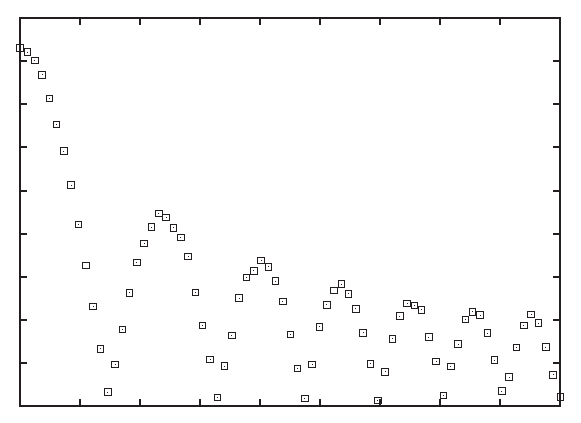
\includegraphics{img/bivariate1}}
  \caption{Data that clearly shows that there is a relationship,
    albeit a complicated one, between $x$ and $y$.}
  \label{fig:bivariate1}\vspace*{-6pt}
\end{figure}\pagebreak

In contrast, Figure \ref{fig:bivariate2} shows the kind of data
typical of much of statistical analysis. Here we might be showing the
prevalence of skin cancer as a function of the mean income for a group
of individuals or the unemployment rate as a function of the frequency
of high-school drop-outs for a number of counties, and the primary
question is whether there is any relationship at all between the two
quantities involved.  The situation here is quite different from that
shown in Figure \ref{fig:bivariate1}, where it was obvious that a
strong relationship existed between $x$ and $y$, and therefore our main
concern was to determine the precise nature of that relationship.

\begin{figure}
  \centerline{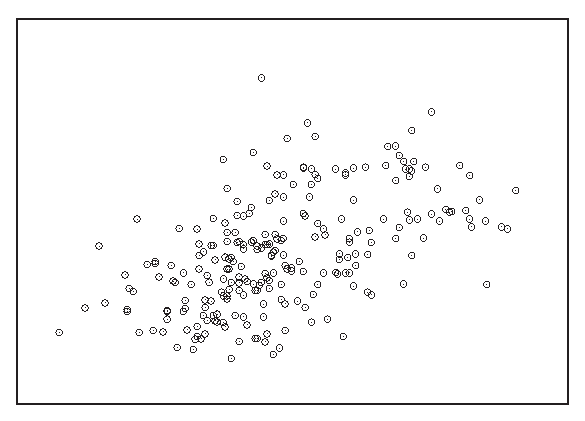
\includegraphics{img/bivariate2}}
  \caption{A noisy data set. Is there any relationship between $x$
    and $y$?}
  \label{fig:bivariate2}\vspace*{12pt}
\end{figure}

A figure such as Figure \ref{fig:bivariate2} is referred to as a
\emph{scatter plot} or \emph{xy plot}. I prefer the latter term
because scatter plot sounds to me too much like ``splatter plot,''
suggesting that the data necessarily will be noisy---but we don't know
that!  Once we plot the data, it may turn out to be very clean and
regular, as in Figure \ref{fig:bivariate1}; hence I am more
comfortable with the neutral term.

\begin{figure}[t!]
  \centerline{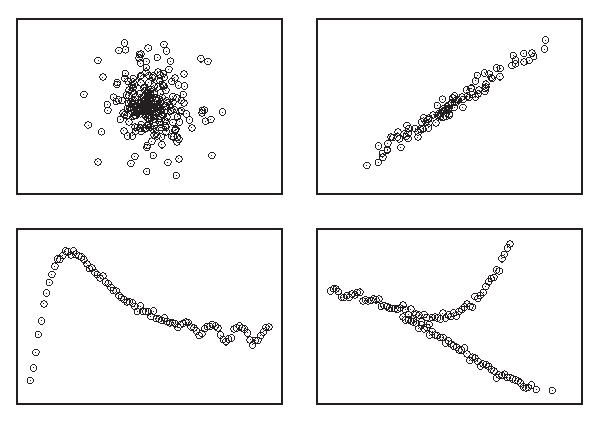
\includegraphics{img/bivariate3}}
  \caption{Four types of functional relationships (left to right, top
    to bottom): no relationship; strong, simple relationship; strong,
    not-simple relationship; multivariate relationship.}
  \label{fig:bivariate3}\vspace*{12pt}
\end{figure}

When we create a graph such as Figure \ref{fig:bivariate1} or Figure
\ref{fig:bivariate2}, we usually want to understand whether there is a
relationship between $x$ and $y$ as well as what the nature of that
relationship is. Figure \ref{fig:bivariate3} shows four different
possibilities that we may find: no relationship; a strong, simple
relationship; a strong, not-simple relationship; and finally a
multivariate relationship (one that is not unique).

% ============================================================
\section{Conquering Noise: Smoothing}

\index{bivariate analysis!noise and smoothing|(}
\index{noise|(}
\index{smoothing|(}
   
When data is noisy, we are more concerned with establishing
\emph{whether} the data exhibits a meaningful relationship, rather\vadjust{\pagebreak}
than establishing its precise character. To see this, it is often
helpful to find a smooth curve that represents the noisy data set.
Trends and structure of the data may be more easily visible from such
a curve than from the cloud of points.

Two different methods are frequently used to provide smooth
representation of noisy data sets: \emph{weighted splines}\index{weighted splines}\index{splines!weighted splines} and
a method known as \emph{LOESS} (or LOWESS), which is short for
locally weighted regression.

Both methods work by approximating the data in a small neighborhood
(\ie, locally) by a polynomial of low order (at most cubic). The trick
is to string the various local approximations together to form a
single smooth curve. Both methods contain an adjustable parameter that
controls the ``stiffness'' of the resulting curve: the stiffer the
curve, the smoother it appears but the less accurately it can follow
the individual data points. Striking the right balance between
smoothness and accuracy is the main challenge when it comes to
smoothing methods.

\spreadlong{-12pt}

\vspace*{-6pt}
\subsection{Splines}

\index{noise!splines}
\index{smoothing!splines}
\index{splines!about} 

Splines are constructed from piecewise polynomial functions \index{polynomials!splines} (typically
cubic) that are joined together in a smooth fashion. In addition to
the local smoothness requirements at each joint, splines must also
satisfy a global smoothness condition by optimizing the functional:\vspace*{-3pt}
%
\[
J[s] = \alpha \int \paren{ \diff[2]{s}{t} }^2 \rms{t}
     + (1-\alpha) \sum_i w_i \paren{ y_i - s(x_i) }^2\vspace*{-3pt}
\]
%
Here $s(t)$ is the spline curve, $(x_i, y_i)$ are the coordinates of
the data points, the $w_i$ are weight factors (one for each data
point), and $\alpha$ is a mixing factor. The first term controls how
``wiggly'' the spline is overall, because the second derivative
measures the curvature of $s(t)$ and becomes large if the curve has
many wiggles. The second term captures how accurately the spline
represents the data points by measuring the squared deviation of the
spline from each data point---it becomes large if the spline does not
pass close to the data points.  Each term in the sum is multiplied by
a weight factor $w_i$, which can be used to give greater weight to
data points that are known with greater accuracy than others. (Put
differently: we can write $w_i$ as $w_i = 1/d_i^2$, where $d_i$
measures how close the spline should pass by $y_i$ at $x_i$.) The
mixing parameter $\alpha$ controls how much weight we give to the
first term (emphasizing overall smoothness) relative to the second
term (emphasizing accuracy of representation).  In a plotting program,
$\alpha$ is usually the dial we use to tune the spline for a given
data set.

% Para below beautiful example of CE inadvertently and subtly changing 
% the semantics. ;-)
To construct the spline explicitly, we form cubic interpolation
polynomials for each consecutive pair of points and require that
these individual polynomials have the same values, as well as the same
first and second derivatives, at the points where they meet. These
smoothness conditions lead to a set of linear equations for the
coefficients in the polynomials, which can be solved. Once these
coefficients have been found, the spline curve can be evaluated at any
desired location.

\subsection{LOESS}

\index{noise!LOESS}
\index{smoothing!LOESS}
\index{LOESS!about|(}
  
Splines have an \emph{overall} smoothness goal, which means that they
are less responsive to \emph{local} details in the data set. The LOESS
smoothing method addresses this concern. It consists of approximating
the data locally through a low-order (typically linear) polynomial \index{polynomials!LOESS} 
(regression), \index{linear regression!LOESS} while weighting all the data points in such a way that
points close to the location of interest contribute more strongly than
do data points farther away (local weighting).

Let's consider the case of first-order (linear) LOESS, so that the local
approximation takes the particularly simple form $a + bx$. To find the
``best fit'' in a least-squares sense, we must minimize:
%
\[
\chi^2 = \sum_i w( x-x_i; h ) \paren{ a + b x_i - y_i }^2
\]
%
with respect to the two parameters $a$ and $b$. Here, $w(x)$ is the
weight function. It should be smooth and strongly peaked---in fact, it
is basically a kernel, similar to those we encountered in Figure
\ref{fig:kernels} when we discussed kernel density estimates.  The
kernel most often used with LOESS is the ``tri-cube'' kernel $K(x) =
\paren{ 1-|x|^3 }^3$ for $|x|<1$, $K(x)=0$ otherwise; but any of the
other kernels will also work.  The weight depends on the distance
between the point $x$ where we want to evaluate the LOESS
approximation and the location of the data points. In addition, the
weight function also depends on the parameter $h$, which controls the
bandwidth of the kernel: this is the primary control parameter for
LOESS approximations.  Finally, the value of the LOESS approximation
at position $x$ is given by $y(x) = a + b x$, where $a$ and $b$
minimize the expression for $\chi^2$ stated earlier.

This is the basic idea behind LOESS. You can see that it is easy to
generalize---for example, to two or more dimensions or two higher-order
approximation polynomials. (One problem, though: explicit, closed
expressions for the parameters $a$ and $b$ can be found only if you
use first-order polynomials; whereas for quadratic or higher
polynomials you will have to resort to numerical minimization
techniques. Unless you have truly compelling reasons, you want to
stick to the linear case!)

LOESS is a computationally intensive method. Keep in mind that the
entire calculation must be performed for \emph{every} point at which
we want to obtain a smoothed value. (In other words, the parameters
$a$ and $b$ that we calculated are themselves functions of $x$.) This
is in contrast to splines: once the spline coefficients have been
calculated, the spline can be evaluated easily at any point that we
wish. In this way, splines provide a summary or approximation to the
data. LOESS, however, does not lend itself easily to semi-analytical
work: what you see is pretty much all you get.

One final observation: if we replace the linear function $a + bx$ in
the fitting process with the constant function $a$, then LOESS becomes
simply a weighted moving average.

\subsection{Examples}

\index{noise!examples|(}
\index{smoothing!examples|(}

Let's look at two examples where smoothing reveals behavior that would
otherwise not be visible.

The first is a famous data set that has been analyzed in many places:
the 1970 draft lottery. \index{draft lottery, LEOSS} During the Vietnam War, men in the
U.S.\ were drafted based on their date of birth. Each possible birth date was
assigned a draft number between 1 and 366 using a lottery process, and
men were drafted in the order of their draft numbers. However,
complaints were soon raised that the lottery was biased---that men
born later in the year had a greater chance of receiving a low draft
number and, consequentially, a greater chance of being drafted
early.\footnote{More details and a description of the lottery process
  can be found in \cit{The Statistical Exorcist}{M.\ Hollander and F.\
    Proschan}{CRC Press}{1984}.}

\begin{figure}
\vspace*{-18pt}
  \centerline{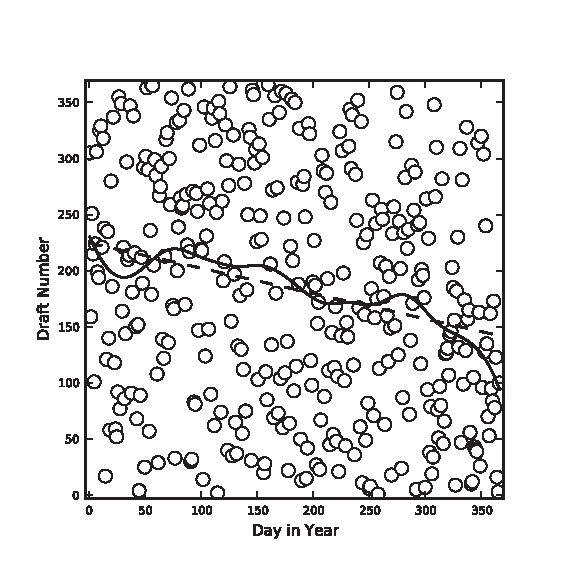
\includegraphics[scale=0.9]{img/draftlottery}}
  \caption{The 1970 draft lottery: draft number versus birth date (the
    latter as given in days since the beginning of the year).  Two
    LOESS curves with different values for the smoothing parameter $h$
    indicate that men born later in the year tended to have lower
    draft numbers. This would not be easily recognizable from a plot
    of the data points alone.}
  \label{fig:draftlottery}\vspace*{-6pt}
\end{figure}

Figure \ref{fig:draftlottery} shows all possible birth dates (as days
since the beginning of the year) and their assigned draft numbers.\vadjust{\pagebreak}  If
the lottery had been fair, these points should form a completely
random pattern. Looking at the data alone, it is virtually impossible
to tell whether there is any structure in the data. However, the
smoothed LOESS lines reveal a strong falling tendency of the draft
number over the course of the year: later birth dates are indeed more
likely to have a lower draft number!

The LOESS lines have been calculated using a Gaussian kernel. \index{Gaussian kernel, LOESS} For the
solid line, I used a kernel bandwidth equal to $5$, but for the dashed
line, I used a much larger bandwidth of $100$. For such a large
bandwidth, practically all points in the data set contribute equally
to the smoothed curve, so that the LOESS operation reverts to a linear
regression of the entire data set. (In other words: if we make the
bandwidth very large, then LOESS amounts to a least-squares fit of a
straight line to the data.)

In this draft number example, we mostly cared about a \emph{global}
property of the data: the presence or absence of an overall trend.
Because we were looking for a global property, a stiff curve (such as
a straight line) was sufficient to reveal what we were looking for.
However, if we want to extract more detail---in particular if we want
to extract \emph{local} features---then we need a ``softer'' curve,
which can follow the data on smaller scales.

Figure \ref{fig:marathon} shows an amusing example.\footnote{This
  example was inspired by \cit{Graphic Discovery: A Trout in the Milk
    and Other Visual Adventures}{Howard Wainer}{2nd ed., Princeton
    University Press}{2007}.} Displayed are the finishing times
(separately for men and women) for the winners in a marathon. Also
shown are the ``best fit'' straight-line approximations for all events
up to 1990. According to this (straight-line) model, women should
start finishing faster than men before the year 2000 and then continue
to become faster at a dramatic rate! This expectation is not borne out
by actual observations: finishing times for women (and men) have
largely leveled off.

\begin{figure}
    \centerline{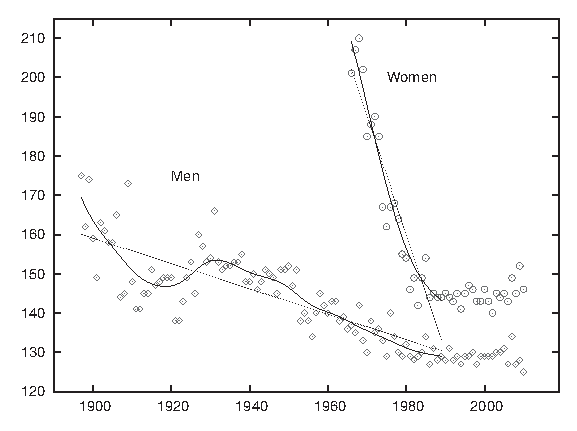
\includegraphics{img/marathon}}
  \caption{Winning times (in minutes) for an annual marathon event,
    separately for men and women. Also shown are the straight-line and
    smooth-curve approximations. All approximations are based entirely
    on data points \emph{prior} to 1990.}
  \label{fig:marathon}
\end{figure}

This example demonstrates the danger of attempting to describe data by
using a model of fixed form (a ``formula'')---and a straight line is
one of the most rigid models out there! A model that is not
appropriate for the data will lead to incorrect conclusions.
Moreover, it may not be obvious that the model is inappropriate. Look
again at Figure \ref{fig:marathon}: don't the straight lines seem
reasonable as a description of the data prior to 1990?

Also shown in Figure \ref{fig:marathon} are smoothed curves calculated
using a LOESS process. Because these curves are ``softer'' they have a
greater ability to capture features contained in the data.  Indeed,
the LOESS curve for the women's results does give an indication that
the trend of dramatic improvements, seen since they first started
competing in the mid-1960s, had already begun to level off before the
year 1990. (All curves are based strictly on data prior to 1990.) This
is a good example of how an adaptive smoothing curve can highlight
local behavior that is present in the data but may not be obvious
from merely looking at the individual data points.

\index{LOESS!about|)}
\index{noise!examples|)}
\index{smoothing!examples|)}

\subsection{Residuals}

\index{noise!residuals}
\index{smoothing!residuals}
\index{residuals, smoothing}

Once you have obtained a smoothed approximation to the data, you will
usually also want to check out the \emph{residuals}---that is, the
remainder when you subtract the smooth ``trend'' from the actual data.

There are several details to look for when studying residuals.

\begin{itemize}
\item Residuals should be balanced: symmetrically distributed around
  zero.
\item Residuals should be free of a trend. The presence of a trend or
  of any other large-scale systematic behavior in the residuals
  suggests that the model is inappropriate! (By construction, this is
  never a problem if the smooth curve was obtained from an adaptive
  smoothing model; however, it is an important indicator if the smooth
  curve comes from an analytic model.)
\item Residuals will necessarily straddle the zero value; they will
  take on both positive and negative values. Hence you may also want
  to plot their absolute values to evaluate whether the overall
  magnitude of the residuals is the same for the entire data set or
  not. The assumption that the magnitude of the variance around a
  model is constant throughout (``homoscedasticity'') \index{homoscedasticity, LOESS} is often an
  important condition in statistical methods. If it is not satisfied,
  then such methods may not apply.
\item Finally, you may want to use a QQ plot \index{QQ plots!LOESS} (see Chapter
  \ref{ch:univariate}) to check whether the residuals are distributed
  according to a Gaussian distribution. This, too, is an assumption
  that is often important for more advanced statistical methods.
\end{itemize}

It may also be useful to apply a smoothing routine to the
\emph{residuals} in order to recognize their features more clearly.
Figure \ref{fig:residuals} shows the residuals for the women's
marathon results (before 1990) both for the straight-line model and
the LOESS smoothing curve. For the LOESS curve, the residuals are
small overall and hardly exhibit any trend. For the straight-line
model, however, there is a strong systematic trend in the residuals
that is increasing in magnitude for years past 1985. This kind of
systematic trend in the residuals is a clear indicator that the model
is not appropriate for the data!

\begin{figure}
  \centerline{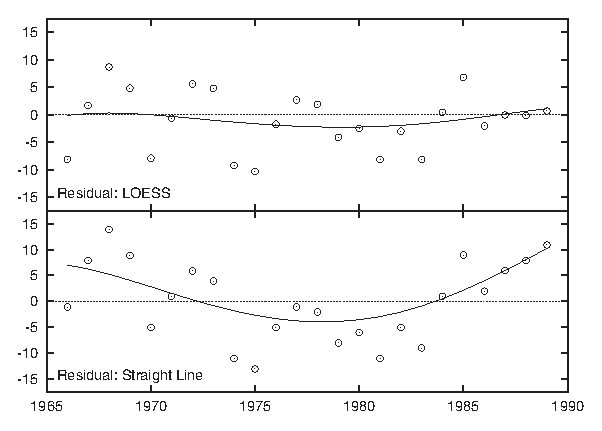
\includegraphics{img/residuals}}
  \caption{Residuals for the women's marathon results, both for the
    LOESS smoothing curve and the straight-line linear regression
    model. The residuals for the latter show an overall systematic
    trend, which suggests that the model does not appropriately
    describe the data.}
  \label{fig:residuals}
\end{figure}

\subsection{Additional Ideas and Warnings}

\index{noise!ideas and warnings}
\index{smoothing!ideas and warnings}

Here are some additional ideas that you might want to play with.

As we have discussed before, you can calculate the residuals between
the real data and the smoothed approximation. Here an isolated large
residual is certainly odd: it suggests that the corresponding data
point is somehow ``different'' than the other points in the
neighborhood---in other words, an outlier. Now we argue as follows.
If the data point is an outlier, then it should contribute less to the
smoothed curve than other points. Taking this consideration into
account, we now introduce an additional weight factor for each data
point into the expression for $J[s]$ or $\chi^2$ given previously.
The magnitude of this weight factor is chosen in such a way that data
points with large residuals contribute less to the smooth curve.  With
this new weight factor reducing the influence of points with large
residuals, we calculate a \emph{new} version of the smoothed
approximation. This process is iterated until the smooth curve no
longer changes.

Another idea is to split the original data points into two classes:
those that give rise to a positive residual and those with a negative
residual. Now calculate a smooth curve for each class separately. The
resulting curves can be interpreted as ``confidence bands'' for the
data set (meaning that the majority of points will lie between the
upper and the lower smooth curve). We are particularly interested to
see whether the width of this band varies along the curve. Figure
\ref{fig:smoothtube} shows an example that uses the men's results from
Figure \ref{fig:marathon}.

\begin{figure}
  \centerline{  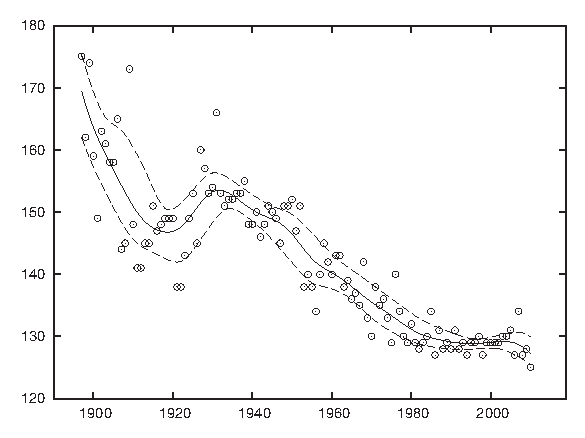
\includegraphics{img/smoothtube}}
  \caption{A ``smooth tube'' for the men's marathon results. The solid
    line is a smooth representation of the entire data set; the dashed
    lines are smooth representations of only those points that lie above
    (or below) the solid line.}
  \label{fig:smoothtube}
\end{figure}

Personally, I am a bit uncomfortable with either of these suggestions.
They certainly have an unpleasant air of circular reasoning about them.

There is also a deeper reason. \index{graphical analysis!interpretation} In my opinion, smoothing methods are a
quick and useful but entirely nonrigorous way to explore the structure
of a data set. With some of the more sophisticated extensions (\eg,
the two suggestions just discussed), we abandon the simplicity of the
approach without gaining anything in rigor! If we need or want better
(or deeper) results than simple graphical methods can give us, isn't
it time to consider a more rigorous toolset?

This is a concern that I have with many of the more sophisticated
graphical methods you will find discussed in the literature. Yes, we
certainly \emph{can} squeeze ever more information into a graph using
lines, colors, symbols, textures, and what have you. But this does not
necessarily mean that we \emph{should}. The primary benefit of a graph
is that it speaks to us directly---without the need for formal
training or long explanations. Graphs that require training or
complicated explanations to be properly understood are missing their
mark no matter how ``clever'' they may be otherwise.

Similar considerations apply to some of the more involved ways of
graph preparation. After all, a smooth curve such as a spline or LOESS
approximation is only a rough approximation to the data set---and, by
the way, contains a huge degree of arbitrariness in the form of the
smoothing parameter ($\alpha$ or $h$, respectively). Given this
situation, it is not clear to me that we need to worry about such
details as the effect of individual outliers on the curve.

Focusing too much on graphical methods may also lead us to miss the
essential point. For example, once we start worrying about confidence
bands, we should really start \emph{thinking more deeply} about the
nature of the local distribution of residuals (Are the residuals
normally distributed? Are they independent? Do we have a reason to
prefer one statistical model over another?)---and possibly consider a
more reliable estimation method (\eg, bootstrapping; see Chapter
\ref{ch:simulation})---rather than continue with hand-waving
(semi-)graphical methods.

Remember: The purpose of computing is insight, not pictures! (L.\ N.\
Trefethen)

\index{bivariate analysis!noise and smoothing|)}
\index{noise|)}
\index{smoothing|)}



% ============================================================
\section{Logarithmic Plots}

\index{bivariate analysis!logarithmic plots|(}
\index{logarithmic plots|(}
  
Logarithmic plots are a standard tool of scientists, engineers, and
stock analysts everywhere. They are so popular because they
have three valuable benefits:

\begin{itemize}
\item They rein in large variations in the data.
\item They turn multiplicative variations into additive ones.
\item They reveal exponential and power law behavior.
\end{itemize}

In a logarithmic plot, we graph the \emph{logarithm} of the data
instead of the raw data. Most plotting programs can do this for us (so
that we don't have to transform the data explicitly) and also take
care of labeling the axes appropriately.

There are two forms of logarithmic plots: \emph{single} or\index{single log plots}
\emph{semi-logarithmic} plots \index{semi-logarithmic plots} and \emph{double logarithmic} \index{double logarithmic plots} or
\emph{log-log} plots, \index{log-log plots} depending whether only one (usually the vertical
or $y$ axis) or both axes have been scaled logarithmically.

All logarithmic plots are based on the fundamental property of the
logarithm to turn products into sums and powers into products:
%
\begin{gather*}
  \log(x y) = \log(x) + \log(y) \\
  \log(x^k) = k \log(x)
\end{gather*}
%
Let's first consider semi-log plots. Imagine you have data generated
by evaluating the function:
%
\[
y = C \exp(\alpha x) \quad \text{where $C$ and $\alpha$ are constants}
\]
%
on a set of $x$ values. If you plot $y$ as a function of $x$, you will
see an upward- or downward-sloping curve, depending on the sign of
$\alpha$ (see Appendix \ref{app:calculus}). But if you instead plot
the \emph{logarithm} of $y$ as a function of $x$, the points will fall
on a straight line. This can be easily understood by applying the
logarithm to the preceding equation:
%
\[
\log y = \alpha x + \log C
\]
%
In other words, the logarithm of $y$ is a linear function of $x$ with
slope $\alpha$ and with offset $\log C$. In particular, by measuring
the slope of the line, we can determine the scale factor $\alpha$,
which is often of great interest in applications.

Figure \ref{fig:semilog} shows an example of a semi-logarithmic plot
that contains some experimental data points as well as an exponential
function for comparison. I'd like to point out a few details. First,
in a logarithmic plot, we plot the logarithm of the values, but the
axes are usually labeled with the actual values (not their
logarithms). Figure \ref{fig:semilog} shows both: the actual values on
the left and the logarithms on the right (the logarithm of 100 to base
10 is 2, the logarithm of 1,000 is 3, and so on). We can see how, in a
logarithmic plot, the logarithms are equidistant, but the actual values
are not. (Observe that the distance between consecutive tick marks is
constant on the right, but not on the left.)

\begin{figure}
  \centerline{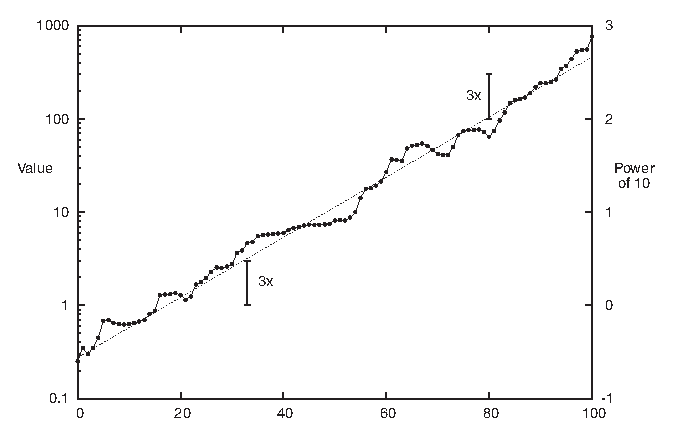
\includegraphics{img/semilog}}
  \caption{A semi-logarithmic plot.}
  \label{fig:semilog}
\end{figure}

Another aspect I want to point out is that on a semi-log plot, all
\emph{relative} changes have the same size no matter how large the
corresponding absolute change. It is this property that makes semi-log
plots popular for long-running stock charts and the like: if you lost
\$100, your reaction may be quite different if originally you had
invested \$1,000 versus \$200: in the first case you lost 10 percent
but 50 percent in the second. In other words, relative change is what
matters.

The two scale arrows in Figure \ref{fig:semilog} have the same length
and correspond to the same relative change, but the underlying
absolute change is quite different (from 1 to 3 in one case, from 100
to 300 in the other). This  is another application of the fundamental
property of the logarithm: if the value before the change is $y_1$ and
if $y_2 = \gamma y_1$ after the change (where $\gamma = 3$), then the
change in absolute terms is:
%
\[
y_2 - y_1 = \gamma y_1 - y_1 = (\gamma - 1) y_1
\]
%
which clearly depends on $y_1$. But if we consider the change
in the logarithms, we find:
%
\[
\log y_2 - \log y_1 
  = \log( \gamma y_1 ) - \log y_1 
  = \log \gamma + \log y_1 - \log y_1
  = \log \gamma
\]
%
which is independent of the underlying value and depends only
on $\gamma$, the size of the relative change.

\begin{figure}
  \centerline{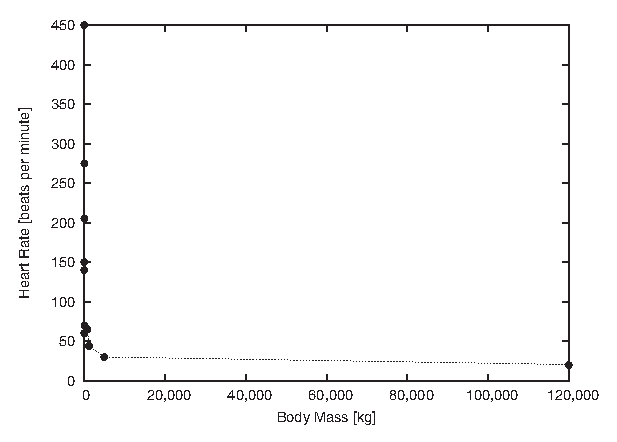
\includegraphics{img/allometric1}}\vspace*{-3pt}
  \caption{Heart rate versus body mass for a range of mammals. Compare
    to Figure \ref{fig:allometric2}.}
  \label{fig:allometric1}\vspace*{-6pt} 
\end{figure}

Double logarithmic plots \index{double logarithmic plots} are now easy to understand---the only
difference is that we plot logarithms of both $x$ \emph{and} $y$.
This will render all power-law relations as straight lines---that is,
as functions of the form $y = C x^k$ or $y = C/x^k$, where $C$ and $k$
are constants. (Taking logarithms on both sides of the first equation
yields $\log y = k \log x + \log C$, so that now $\log y$ is a linear
function of $\log x$ with a slope that depends on the exponent $k$.)

Figures \ref{fig:allometric1} and \ref{fig:allometric2} provide
stunning example for both uses of double logarithmic plots: their
ability to render data spanning many order of magnitude accessible and
their ability to reveal power-law relationships by turning them into
straight lines. Figure \ref{fig:allometric1} shows the typical resting
heart rate (in beats per minute) as a function of the body mass (in
kilograms) for a selection of mammals from the hamster to large 
whales. Whales weigh in at 120 tons---nothing else even comes close!
The consequence is that almost all of the data points are squished
against the lefthand side of the graph, literally crushed by the
whale.



On the double logarithmic plot, the distribution of data points
becomes much clearer. Moreover, we find that the data points are not
randomly distributed but instead seem to fall roughly on a straight
line with slope $-1/4$: the signature of power-law behavior. In other
words, a mammal's typical heart rate is related to its mass: larger
animals have slower heart beats. If we let $f$ denote the heart rate
and $m$ the mass, we can summarize this observation as:
%
\[
f \sim m^{-1/4}
\]

\begin{figure}
  \centerline{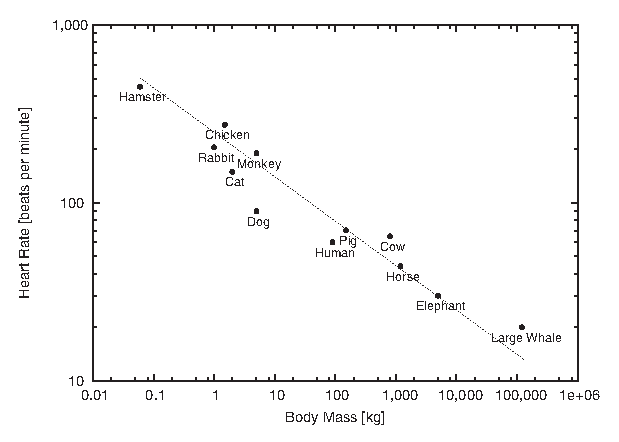
\includegraphics{img/allometric2}}
  \caption{The same data as in Figure \ref{fig:allometric1} but now
    plotted on a double logarithmic plot. The data points seem to fall
    on a straight line, which indicates a power-law relationship
    between resting heart rate and body mass.}
  \label{fig:allometric2} \vspace*{-6pt}
\end{figure}

This surprising result is known as \emph{allometric scaling}. \index{allometric scaling} It seems
to hold more generally and not just for the specific animals and
quantities shown in these figures. (For example, it turns out that the
lifetime of an individual organism also obeys a $1/4$ power-law
relationship with the body mass: larger animals live longer. The
surprising consequence is that the total number of heartbeats per life
of an individual is approximately constant for all species!)
Allometric scaling has been explained in terms of the geometric
constraints of the vascular network (veins and arteries), which brings
nutrients to the cells making up a biological system.  It is
sufficient to assume that the network must be a space-filling fractal,
that the capillaries where the actual exchange of nutrients takes
place are the same size in all animals, and that the overall energy
required for transport  through the  network is
minimized, to derive the power-law relationships observed experimentally!\footnote{The
original
  reference is \pcit{A General Model for the Origin of Allometric Scaling
  Laws in Biology}{\newline G.~B.\ West, J.\ H.\ Brown, and B.\ J.\
  Enquist}{Science}{276}{1997}{122} Additional references
  can be found on the Web.}  We'll have more to say about scaling laws
and their uses in Part \ref{part:analytics}.

% --- XXX : Here, I had the log-histo discussion, now removed. Reinstate?

\index{bivariate analysis!logarithmic plots|)}
\index{logarithmic plots|)}

% ============================================================

\setcounter{footnote}{1}
\section{Banking}

\index{bivariate analysis!banking|(}
\index{banking|(} 

Smoothing methods and logarithmic plots are both tools that help us 
recognize structure in a data set. Smoothing methods reduce noise, and
logarithmic plots help with data sets spanning many orders of
magnitude.

Banking (or ``banking to 45 degrees'') is another graphical method.
It is different than the preceding ones because it does not work on
the \emph{data} but on the plot as a whole by changing its aspect
ratio.

We can recognize \emph{change} (\ie, the slopes of curves) most
easily if they make approximately a 45 degree angle on the graph. It
is much harder to see change if the curves are nearly horizontal or
(even worse) nearly vertical. The idea behind \emph{banking} is
therefore to adjust the aspect ratio of the entire plot in such a way
that most slopes are at an approximate 45 degree angle. 

Chances are, you have been doing this already by changing the plot
\emph{ranges}. Often when we ``zoom'' in on a graph it's not so much
to see more detail as to adjust the slopes of curves to make them more
easily recognizable. The purpose is even more obvious when we zoom
\emph{out}. Banking is a more suitable technique to achieve the same
effect and opens up a way to control the appearance of a plot by
actively adjusting the aspect ratio.\index{aspect ratios, banking}

Figures \ref{fig:sunspot1} and \ref{fig:sunspot2} show the classical
example for this technique: the annual number of sunspots measured
over the last 300 years.\footnote{The discussion here is adapted from my
  book \emph{Gnuplot in Action}. Manning Publications. 2010.}  In
Figure \ref{fig:sunspot1}, the oscillation is very compressed, and so
it is difficult to make out much detail about the shape of the curve.
In Figure \ref{fig:sunspot2}, the aspect ratio of the plot has been
adjusted so that most line segments are now at roughly a 45 degree
angle, and we can make an interesting observation: the rising edge of
each sunspot cycle is steeper than the falling edge. We would probably
not have recognized this by looking at Figure \ref{fig:sunspot1}.

\begin{figure}
  \centerline{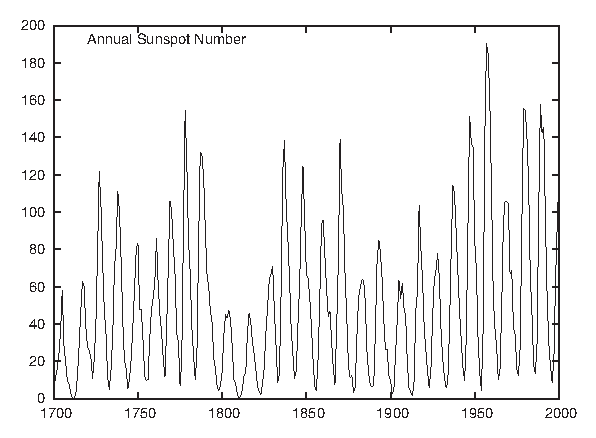
\includegraphics{img/sunspot1}}
  \caption{The annual sunspot numbers for the last 300 years. The
    aspect ratio of the plot makes it hard to recognize the details of
    each cycle.}
  \label{fig:sunspot1}%\vspace*{-12pt}
\end{figure}

\begin{figure}
  \centerline{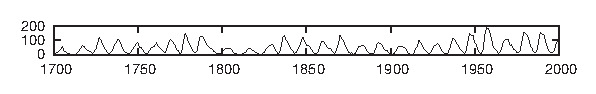
\includegraphics{img/sunspot2}}
  \caption{The same data as in Figure \ref{fig:sunspot1}. The aspect
    ratio has been changed so that rising and falling flanks of the
    curve make approximately a 45 degree angle with the horizontal
    (banking to 45 degrees), but the figure has become so small that
    it is hard to recognize much detail.}
  \label{fig:sunspot2}\vspace*{-6pt}
\end{figure} 

Personally, I would probably not use a graph such as Figure
\ref{fig:sunspot2}: shrinking the vertical axis down to almost nothing
loses too much detail. It also becomes difficult to compare the
behavior on the far left and far right of the graph. Instead, I would
break up the time series and plot it as a \emph{cut-and-stack plot},
such as the one in Figure \ref{fig:sunspot3}. Note that in this plot
the aspect ratio of each subplot is such that the lines are, in fact,
banked to 45 degrees.

As this example demonstrates, banking is a good technique but can be
taken too literally. When the aspect ratio required to achieve proper
banking is too skewed, it is usually better to rethink the entire
graph. No amount of banking will make the data set in 
Figure~\ref{fig:allometric1} look right---you need a double logarithmic
transform.

There is also another issue to consider.  The purpose of banking is to
improve human perception of the graph (it is, after all, exactly the\vadjust{\pagebreak}
same data that is displayed). But graphs with highly skewed aspect
ratios violate the great affinity humans seem to have for proportions
of roughly 4 by 3 (or 11 by 8.5 or $\sqrt{2}$ by $1$). Witness the
abundance of display formats (paper, books, screens) that adhere
approximately to these proportions the world over. Whether we favor
this display format because we are so used to it or (more likely, I
think) it is so predominant because it works well for humans is rather
irrelevant in this context. (And keep in mind that squares seem to
work particularly badly---notice how squares, when used for furniture
or appliances, are considered a ``bold'' design.  Unless there is a
good reason for them, such as graphing a square matrix, I recommend
you avoid square displays.)

\index{bivariate analysis!banking|)}
\index{banking|)} 

\begin{figure}
  \centerline{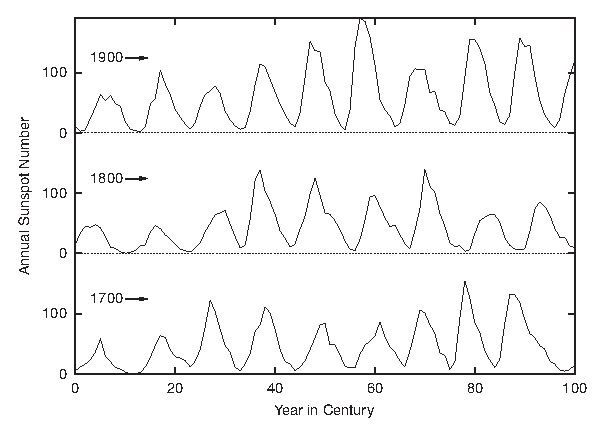
\includegraphics{img/sunspot3}}
  \caption{A cut-and-stack plot of the data from Figure
    \ref{fig:sunspot1}.  By breaking the time axis into three chunks,
    we can bank each century to 45 degrees and still fit all the data
    into a standard-size plot.  Note how we can now easily recognize
    an important feature of the data: the rising flank tends to be
    steeper than the falling one.}
  \label{fig:sunspot3}
\end{figure}

\vspace*{-6pt}
% ============================================================
\section{Linear Regression and All That}

\index{bivariate analysis!linear regression|(} 
\index{linear regression!about|(}
 
Linear regression is a method for finding a straight line through
a two-dimensional scatter plot. It is simple to calculate and
has considerable intuitive appeal---both of which together make
it easily the single most-often misapplied technique in all of
statistics!

There is a fundamental misconception regarding linear
regression---namely that it is a good and particularly rigorous way to
\emph{summarize}\vadjust{\pagebreak} the data in a two-dimensional scatter plot.  This
misconception is often associated with the notion that linear
regression provides the ``best fit'' to the data.

This is not so. Linear regression is not a particularly good way to 
summarize data, and it provides a ``best fit'' in a much more limited
sense than is generally realized. 

Linear regression applies to situations where we have a set of input
values (the controlled variable) and, for each of them, we measure an
output value (the response variable).  Now we are looking for a linear
function $f(x) = a + b x$ as a function of the controlled variable $x$
that reproduces the response with the least amount of error. The
result of a linear regression is therefore a function that minimizes
the error in the responses for a given set of inputs.

This is an important understanding: the purpose of a regression
procedure is not to \emph{summarize} the data---the purpose is to
obtain a function that allows us to \emph{predict} the value of the
response variable (which is affected by noise) that we expect for a
certain value of the input variable (which is assumed to be known
exactly).

\begin{figure}
  \centerline{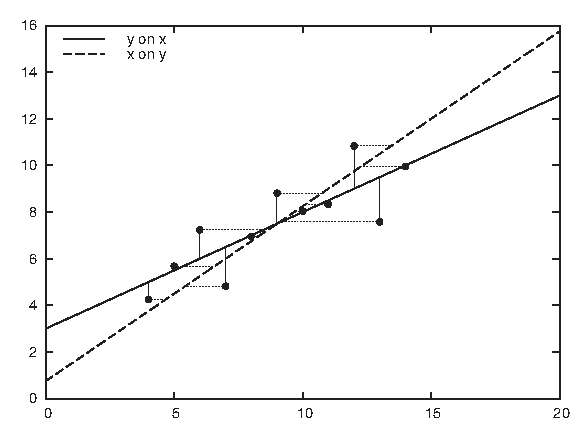
\includegraphics{img/regressionxy}}
  \caption{The first data set from Anscombe's quartet (Table
    \ref{tbl:anscombe}), fit both ways: $y = a + bx$ and $x = c + d
    y$. The thin lines indicate the errors, the squares of which are
    summed to give $\chi^2$. Depending on what you consider the input
    and the response variable, the ``best fit'' turns out to be
    different!}
  \label{fig:regressionxy}
\end{figure}

As you can see, there is a fundamental asymmetry between the two
variables: the two are not interchangeable.  In fact, you will obtain
a \emph{different} solution when you regress $x$ on $y$ than when you
regress $y$ on $x$. Figure \ref{fig:regressionxy} demonstrates this
effect: the same data set is fitted both ways: $y = a + bx$ and $x = c
+ d y$. The resulting straight lines are quite different.

This simple observation should dispel the notion that linear
regression provides \emph{the} best fit---after all, how could there
be two different ``best fits'' for a single\vadjust{\pagebreak} data set? Instead, linear
regression provides the most faithful representation of an output in
response to an input. In other words, \emph{linear regression is not
  so much a best fit as a best predictor}.

How do we find this ``best predictor''? We require it to minimize the
error in the responses, so that we will be able to make the most
accurate predictions.  But the error in the responses is simply the
sum over the errors for all the individual data points. Because errors
can be positive or negative (as the function over- or undershoots the
real value), they may cancel each other out. To avoid this, we do not sum
the errors themselves but their squares:
%
\begin{align*}
\chi^2 & = \sum_i \paren{ f(x_i) - y_i }^2 \\
       & = \sum_i \paren{ a + b x_i - y_i }^2
\end{align*}
%
where $(x_i, y_i)$ with $i=1 \dots n$ are the data points.  Using the
values for the parameters $a$ and $b$ that minimize this quantity will
yield a function that best explains $y$ in terms of $x$.

\begin{figure}
    \centerline{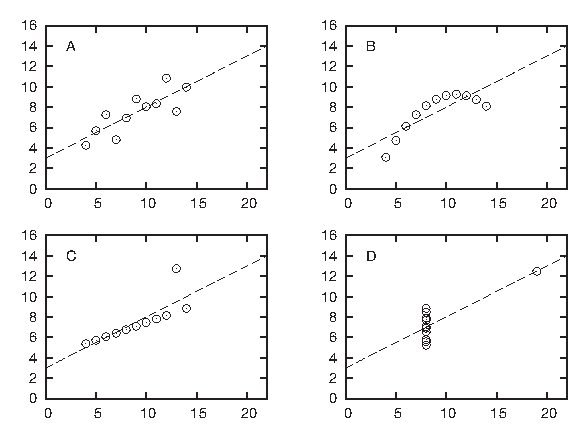
\includegraphics{img/anscombe}}
  \caption{Anscombe's quartet: all summary statistics (in particular
    the regression coefficients) for all four data sets are
    numerically equal, yet only data set A is well represented by the
    linear regression function.}
  \label{fig:anscombe}
\end{figure}

\begin{table}
\def\vrl{\smash{\vrule height124.5pt width.25pt depth3pt}}%
\def\vvrl{\smash{\vrule height138.5pt width.25pt depth3pt\hskip2pt\vrule height138.5pt width.25pt depth3pt}}%
\tbl{Anscombe's quartet.}{%
%\begin{center}
\begin{tabular}{@{\hskip6pt}r@{\hskip6pt}c@{\hskip-2pt}r@{\hskip6pt}c@{\hskip-2pt}r@{\hskip6pt}c@{\hskip-2pt}r@{\hskip6pt}c@{\hskip-2pt}r@{\hskip6pt}c@{\hskip-2pt}r@{\hskip6pt}c@{\hskip-2pt}r@{\hskip6pt}c@{\hskip-2pt}r@{\hskip6pt}}
\toprule
\multicolumn{2}{@{\hskip24pt}c@{\hskip-6pt}}{\TCH{A}} &&   \multicolumn{4}{c}{\TCH{B}} &&  \multicolumn{3}{c}{\TCH{C}} &&  \multicolumn{3}{c}{\TCH{D}} \\
\colrule
\multicolumn{1}{c}{\TCH{\itshape x}} & & \multicolumn{1}{c}{\TCH{\itshape y}} &&
\multicolumn{1}{c}{\TCH{\itshape x}} && \multicolumn{1}{c}{\TCH{\itshape y}} &&
\multicolumn{1}{c}{\TCH{\itshape x}} && \multicolumn{1}{c}{\TCH{\itshape y}} &&
\multicolumn{1}{c}{\TCH{\itshape x}} && \multicolumn{1}{c}{\TCH{\itshape y}} \\\colrule
10.0  && 8.04   && 10.0 && 9.14   && 10.0 && 7.46   && 8.0  && 6.58  \\ 
8.0   && 6.95   && 8.0  && 8.14   && 8.0  && 6.77   && 8.0  && 5.76  \\
13.0  && 7.58   && 13.0 && 8.74  && 13.0  && 12.74  && 8.0  && 7.71  \\
9.0   && 8.81   && 9.0  && 8.77   && 9.0  && 7.11   && 8.0  && 8.84  \\
11.0  && 8.33   && 11.0 && 9.26   && 11.0 && 7.81   && 8.0  && 8.47  \\
14.0  && 9.96   && 14.0 && 8.10   && 14.0 && 8.84   && 8.0  && 7.04  \\
6.0   && 7.24   && 6.0  && 6.13   && 6.0  && 6.08   && 8.0  && 5.25  \\
4.0   && 4.26   && 4.0  && 3.10   && 4.0  && 5.39   && 19.0 && 12.50 \\
12.0  && 10.84  && 12.0 && 9.13   && 12.0 && 8.15   && 8.0  && 5.56  \\
7.0   && 4.82   && 7.0  && 7.26   && 7.0  && 6.42   && 8.0  && 7.91  \\
5.0   &\vrl& 5.68   &\vvrl& 5.0  &\vrl& 4.74   &\vvrl& 5.0  &\vrl& 5.73   &\vvrl& 8.0  &\vrl& 6.89  \\
%\hline
\end{tabular}}\vspace*{6pt}
%\end{center} 
  \label{tbl:anscombe}
\end{table}

Because the dependence of $\chi^2$ on $a$ and $b$ is particularly
simple, we can work out expressions for the optimal choice of both
parameters explicitly. The results are:
%
\begin{gather*}
b = \frac{n \sum x_i y_i - \paren{\sum x_i} \paren{\sum y_i} }
         {n \paren{\sum x_i^2} - \paren{\sum x_i}^2 } \\
a = \frac{1}{n} \paren{\sum y_i - b \sum x_i}
\end{gather*}
%
These results are simple and beautiful---and, in their simplicity,
very suggestive. But they can also be highly misleading.  Table
\ref{tbl:anscombe} and Figure \ref{fig:anscombe} show a famous
example, \emph{Anscombe's quartet}. \index{Anscombe's Quartet} If you calculate the
regression coefficients $a$ and $b$ for each of the four data sets shown in Table
\ref{tbl:anscombe}, you will find that they are exactly the same for
all four data sets! Yet when you look at the corresponding scatter
plots, it is clear that only the first data set is properly described
by the linear model. The second data set is not linear, the third is
corrupted by an outlier, and the fourth does not contain enough
independent $x$ values to form a regression at all! Looking only at
the results of the linear regression, you would never know this.

 

I think this example should demonstrate once and for all how dangerous
it can be to rely on linear regression (or on any form of aggregate
statistics) to summarize a data set. (In fact, the situation is even
worse than what I have presented: with a little bit more work, you can
calculate confidence intervals on the linear regression results, and
even \emph{they} turn out to be equal for all four members of
Anscombe's quartet!)

Having seen this, here are some questions to ask \emph{before}
computing linear regressions.

\begin{unnumlist}
\mysubparagraph{Do you need regression?}
\item Remember that regression coefficients
  are not a particularly good way to \emph{summarize} data. Regression
  only makes sense when you want to use it for \emph{prediction}. If
  this is not the case, then calculating regression coefficients is not
  useful.

\mysubparagraph{Is the linear assumption appropriate?}
\item Linear regression is 
  appropriate only if the data can be described by a straight line.
  If this is obviously not the case (as with the second data set in
  Anscombe's quartet), then linear regression does not apply. 

\mysubparagraph{Is something else entirely going on?} 
\item
Linear regression,
  like all summary statistics, can be led astray by outliers or
  other ``weird'' data sets, as is demonstrated by the last two
  examples in Anscombe's quartet. 
\end{unnumlist}

Historically, one of the attractions of linear regression has been
that it is easy to calculate: all you need to do is to calculate the
four sums $\sum x_i$, $\sum x_i^2$, $\sum y_i$, and $\sum x_i y_i$,
which can be done in a single pass through the data set. Even with
moderately sized data sets (dozens of points), this is arguably easier
than plotting them using paper and pencil! However, that argument
simply does not hold anymore: graphs are easy to produce on a computer
and contain so much more information than a set of regression
coefficients that they should be the preferred way to analyze,
understand, and summarize data.

Remember: The purpose of computing is insight, not numbers! (R.\ W.\
Hamming)

\index{bivariate analysis!linear regression|)} 
\index{linear regression!about|)}
\vspace*{-9pt}
% ============================================================
\section{Showing What's Important}

\index{graphical analysis!process}

Perhaps this is a good time to express what I believe to be the most
important principle in graphical analysis:

% \emph{Show what you want to see!}
\emph{Plot the pertinent quantities!}

As obvious as it may appear, this principle is often overlooked in
practice.

For example, if you look through one of those books that show and
discuss examples of poor graphics, you will find that most examples
fall into one of two classes. First, there are those graphs that
failed \emph{visually}, with garish fonts, unhelpful symbols, and
useless embellishments. (These are mostly presentation graphics gone
wrong, not examples of bad graphical analysis.)

The second large class of graphical failures consists of those plots
that failed \emph{conceptually} or, one might better say,
\emph{analytically}. The problem\vadjust{\pagebreak} with these is not in the technical
aspects of drawing the graph but in the conceptual understanding of
what the graph is trying to show. These plots displayed something, but
they failed to present what was most important or relevant to the
question at hand.

The problem, of course, is that usually it is not at all obvious
\emph{what} we want to see, and it is certainly not obvious at the
beginning. It usually takes several iterations, while a mental model
of the data is forming in your head, to articulate the proper question
that a data set is suggesting and to come up with the best way of
answering it.  This typically involves some form of transformation or
manipulation of the data: instead of the raw data, maybe we should
show the difference between two data sets. Or the residual after
subtracting a trend or after subtracting the results from a model. Or
perhaps we need to normalize data sets from different sources by
subtracting their means and dividing by their spreads. Or maybe we
should not use the original variables to display the data but instead
apply some form of transformation on them (logarithmic scales are only
the simplest example of such transformations). Whatever we choose to
do, it will typically involve some form of transformation of the
data---it's rarely the raw data that is most interesting; but any
deviation from the expected is almost always an interesting discovery.

Very roughly, I think we can identify a three-step (maybe four-step)  
process. It should be taken not in the sense of a prescriptive
checklist but rather in the sense of a gradual process of learning and
discovery.

\myparagraph{First: The basics.} Initially, we are mostly concerned with
displaying what is there.
\begin{itemize}
\item Select proper ranges.
\item Subtract a constant offset.
\item Decide whether to use symbols (for scattered data), lines (for
  continuous data), or perhaps both (connecting individual symbols
  can help emphasize trends in sparse data sets).
\end{itemize}

\myparagraph{Second: The appearance.} Next, we work with aspects of the
plot that influence its overall appearance.
\begin{itemize}
\item Log plots.
\item Add a smoothed curve.
\item Consider banking.
\end{itemize}

\myparagraph{Third: Build a model.} At this point, we start building a
mathematical model and compare it against the raw data. The comparison
often involves finding the differences between the model and the data
(typically subtracting the model or forming a ratio).
\begin{itemize}
\item Subtract a trend.
\item Form the ratio to a base value or baseline.
\item Rescale a set of curves to collapse them onto each other.
\end{itemize}

\myparagraph{Fourth (for presentation graphics only): Add embellishments.} Embellishments 
and decorations (labels, arrows, special symbols, explanations, and so
on) can make a graph much more informative and self-explanatory.
However, they are intended for an audience beyond the actual creator
of the graph. You will rarely need them during the \emph{analysis}
phase, when you are trying to find out something new about the data
set, but they are an essential part when \emph{presenting} your
results. This step should only occur if you want to communicate your
results to a wider and more general audience.

% ============================================================
\section{Graphical Analysis and Presentation Graphics}

\index{graphical analysis!defined}
\index{presentation graphics, defined} 
 
I have used the terms \emph{graphical analysis} and \emph{presentation
  graphics} without explaining them properly. In short:

\begin{unnumlist}
\mysubparagraph{Graphical analysis}
\item Graphical analysis is an investigation of
  data using graphical methods. The purpose is the discovery of
  \emph{new} information about the underlying data set. In graphical
  analysis, the proper question to ask is often not known at the
  outset but is discovered as part of the analysis.

\mysubparagraph{Presentation graphics}
\item Presentation graphics are concerned with
  the communication of information and results that are \emph{already
    understood}. The discovery has been made, and now it needs to be
  communicated clearly.
\end{unnumlist}

The distinction between these two activities is important, because
they do require different techniques and yield different work products.

During the analysis process, convenience and ease of use are the
predominant concerns---any amount of polishing is too much! Nothing
should keep you from redrawing a graph, changing some aspect of it,
zooming in or out, applying transformations, and changing styles.
(When working with a data set I haven't seen before, I probably create
dozens of graphs within a few minutes---basically, ``looking at the
data from all angles.'')  At this stage, any form of embellishment
(labels, arrows, special symbols) is inappropriate---you know what you
are showing, and creating any form of decoration on the graph will
only make you more reluctant to throw the graph away and start over.

For presentation graphics, the opposite applies. Now you already
know the results, but you would like to communicate them to others.
Textual information therefore becomes very important: how else will
people know what they are looking at?

You can find plenty of advice elsewhere on how to prepare ``good''
presentation graphics---often strongly worded and   with an
unfortunate tendency to use emotional responses (ridicule or derision)
in place of factual arguments.  In the absence of good empirical
evidence one way or the other, I will not add to the discussion. But I
present a \emph{checklist} below, mentioning some points that are
often overlooked when preparing graphs for presentation:
\begin{itemize}
\item Try to make the text self-explanatory. Don't rely on a (separate)
  caption for basic information---it might be removed during 
  reproduction. Place basic information on the graph itself.

\item Explain what is plotted on the axes. This can be done with 
  explicit labels on the axes or through explanatory text elsewhere.
  Don't forget the units!

\item Make labels self-explanatory. Be careful with nonstandard
  abbreviations. Ask yourself: If this is all the context provided,
  are you \emph{certain} that the reader will be able to figure out
  what you mean? (In a recent book on data graphing, I found a
  histogram labeled \emph{Married}, \emph{Nvd}, \emph{Dvd},
  \emph{Spd}, and \emph{Wdd}. I could figure out most of them, because
  at least \emph{Married} was given in long form, but I struggled with
  \emph{Nvd} for quite a while!)

\item Given how important \emph{text} is on a graph, make sure to pick
  a suitable font. Don't automatically rely on the default provided by
  your plotting software. Generally, sans-serif fonts (such as
  Helvetica) are preferred for short labels, such as those on a graph,
  whereas serif fonts (such as Times) are more suitable for body text.
  Also pick an appropriate size---text fonts on graphics are often too
  large, making them look garish. (Most text fonts are used at
  10-point to 12-point size; there is no need for type on graphics to
  be much larger.)

\item If there are error bars, be sure to explain their meaning. What
  are they: standard deviations, inter-quartile ranges, or the limits
  of experimental apparatus? Also, choose an appropriate measure of
  uncertainty. Don't use standard deviations for highly skewed data.

\item Don't forget the basics. Choose appropriate plot ranges. Make
  sure that data is not unnecessarily obscured by labels.

\item Proofread graphs! Common errors include: typos in textual
  labels, interchanged data sets or switched labels, missing units,
  and incorrect order-of-magnitude qualifiers (\eg, milli- versus
  micro-).

\item Finally, choose an appropriate output format for your graph!
  Don't use bitmap formats (GIF, JPG, PNG) for print publication---use
  a scalable format such as PostScript or PDF.
\end{itemize}

One last piece of advice: creating good presentation graphics is also
a matter of \emph{taste}, and taste can be acquired. If you want to
work with data, then you should develop an interest in graphs---not
just the ones you create yourself, but all that you see. If you notice
one that seems to work (or not), take a moment to figure out what
makes it so. Are the lines too thick? The labels too small? The choice
of colors just right? The combination of curves helpful? Details
matter.

% ============================================================
\section{Workshop: matplotlib}

\index{bivariate analysis!matplotlib|(}
\index{matplotlib|(}
  
The matplotlib module is a Python module for creating two-dimensional
$xy$ plots, scatter plots, and other plots typical of scientific
applications. It can be\vadjust{\pagebreak} used in an interactive session (with the plots
being shown immediately in a GUI window) or from within a script to
create graphics files using common graphics file formats.

Let's first look at some examples to demonstrate how matplotlib can be
used from within an interactive session. Afterward, we will take a
closer look at the structure of the library and give some pointers for
more detailed investigations.

\subsection{Using matplotlib Interactively}

\index{matplotlib!using interactively|(}
 
To begin an interactive matplotlib session, start IPython (the enhanced
interactive Python shell) with the \texttt{-pylab} option, entering
the following command line like at the shell prompt:

\begin{verbatim}
ipython -pylab  
\end{verbatim}

This will start IPython, load matplotlib \emph{and} NumPy, and import
both into the global namespace. The idea is to give a Matlab-like
experience of interactive graphics together with numerical and matrix
operations.  (It is important to use IPython here---the flow of
control between the Python command interpreter and the GUI eventloop
for the graphics windows requires it. Other interactive shells can be
used, but they may require some tinkering.)

We can now create plots right away:

\begin{verbatim}
In [1]: x = linspace( 0, 10, 100 )

In [2]: plot( x, sin(x) )
Out[2]: [<matplotlib.lines.Line2D object at 0x1cfefd0>]
\end{verbatim}

This will pop up a new window, showing a graph like the one in Figure
\ref{fig:mplt1} but decorated with some GUI buttons. (Note that the
\texttt{sin()} function is a ufunc from the NumPy package: it takes a
vector and returns a vector of the same size, having applied the sine
function to each element in the input vector. See the Workshop in
Chapter \ref{ch:univariate}.)

\begin{figure}
  \centerline{ 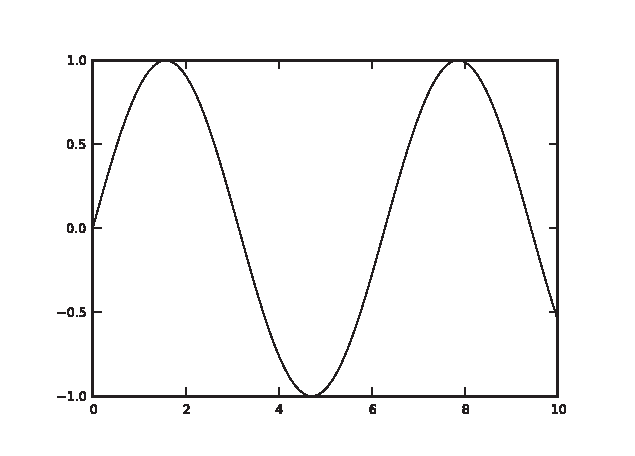
\includegraphics{img/mplt1}}
  \caption{A simple matplotlib figure (see text).}
  \label{fig:mplt1}
\end{figure}

We can now add additional curves and decorations to the plot. Continuing
in the same session as before, we add another curve and some labels:

\begin{verbatim}
In [3]: plot( x, 0.5*cos(2*x) )
Out[3]: [<matplotlib.lines.Line2D object at 0x1cee8d0>]

In [4]: title( "A matplotlib plot" )
Out[4]: <matplotlib.text.Text object at 0x1cf6950>

In [5]: text( 1, -0.8, "A text label" )
Out[5]: <matplotlib.text.Text object at 0x1f59250>

In [6]: ylim( -1.1, 1.1 )
Out[6]: (-1.1000000000000001, 1.1000000000000001)
\end{verbatim}

In the last step, we increased the range of values plotted on the
vertical axis. (There is also an \texttt{axis()} command, which allows
you to specify limits for both axes at the same time. Don't confuse it
with the \texttt{axes()} command, which creates a new coordinate
system.) The plot should now look like the one in Figure
\ref{fig:mplt2}, except that in an interactive terminal the different
lines are distinguished by their color, not their dash pattern.



% not really interactive - limits get reset!

Let's pause for a moment and point out a few details. First of all,
you should have noticed that the graph in the plot window was updated
after every operation. That is typical for the interactive mode, but it
is not how matplotlib works in a script: in general, matplotlib tries
to delay the (possibly expensive) creation of an actual plot until the
last possible moment. (In a script, you would use the \texttt{show()}
command to force generation of an actual plot window.)


\begin{figure}
   \centerline{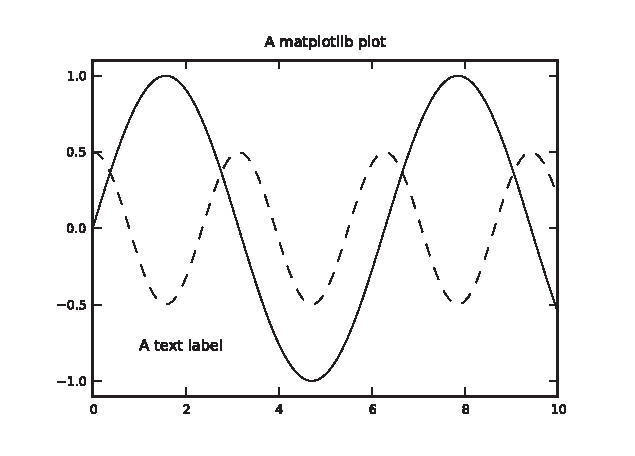
\includegraphics{img/mplt2}}
  \caption{The plot from Figure \ref{fig:mplt1} with an additional
    curve and some decorations added.}
  \label{fig:mplt2}\vspace*{-18pt}
\end{figure}

Furthermore, matplotlib is ``stateful'': a new plot command does not
erase the previous figure and, instead, adds to it. This behavior can
be toggled with the \texttt{hold()} command, and the current state can
be queried using \texttt{ishold()}. (Decorations like the text labels
are not affected by this.) You can clear a figure explicitly using
\texttt{clf()}.

This implicit state may come as a surprise: haven't we learned to make
things explicit, when possible? In fact, this stateful behavior is a
holdover from the way Matlab works. Here is another example. Start a
new session and execute the following commands:

\begin{verbatim}
In [1]: x1 = linspace( 0, 10, 40 )

In [2]: plot( x1, sqrt(x1), 'k-' )
Out[2]: [<matplotlib.lines.Line2D object at 0x1cfef50>]
\end{verbatim}

\begin{verbatim}
In [3]: figure(2)
Out[3]: <matplotlib.figure.Figure object at 0x1cee850>

In [4]: x2 = linspace( 0, 10, 100 )

In [5]: plot( x1, sin(x1), 'k--', x2, 0.2*cos(3*x2), 'k:' )
Out[5]: 
[<matplotlib.lines.Line2D object at 0x1fb1150>,
 <matplotlib.lines.Line2D object at 0x1fba250>]

In [6]: figure(1)
Out[6]: <matplotlib.figure.Figure object at 0x1cee210>

In [7]: plot( x1, 3*exp(-x1/2), linestyle='None', color='white', marker='o', 
   ...: markersize=7 )
Out[7]: [<matplotlib.lines.Line2D object at 0x1d0c150>]

In [8]: savefig( 'graph1.png' )
\end{verbatim}

This snippet of code demonstrates several things. We begin as before,
by creating a plot. This time, however, we pass a third argument to
the \texttt{plot()} command that controls the appearance of the graph
elements. That matplotlib library supports Matlab-style mnemonics for
plot styles; the letter \texttt{k} stands for the color ``black'' and
the single dash \texttt{-} for a solid line. (The letter \texttt{b}
stands for ``blue.'')

Next we create a second figure in a new window and switch to it by
using the \texttt{figure(2)} command. All graphics commands will now
be directed to this second figure---until we switch back to the
first figure using \texttt{figure(1)}. This is another example of
``silent state.'' Observe also that figures are counted starting from 1,
not from 0.

In line 5, we see another way to use the plot command---namely, by
specifying two sets of curves to be plotted together. (The formatting
commands request a dashed and a dotted line, respectively.) Line 7
shows yet a different way to specify plot styles: by using named
(keyword) arguments.

Finally, we save the currently active plot (\ie, figure 1) to a
PNG file. The \texttt{savefig()} function determines the desired
output format from the extension of the filename given. Other formats
that are supported out of the box are PostScript, PDF, and SVG.
Additional formats may be available, depending on the libraries
installed on your system.

\index{matplotlib!using interactively|)}

\subsection{Case Study: LOESS with matplotlib}
\index{matplotlib!LOESS case study}
\index{LOESS!matplotlib case study}  
As a quick example of how to put the different aspects of matplotlib
together, let's discuss the script used to generate Figure
\ref{fig:draftlottery}. This also gives us an opportunity to look at
the LOESS method in a bit more detail.

To recap: LOESS stands for \emph{locally weighted} linear regression.\index{linear regression!LOESS}
The difference between LOESS and regular linear regression is the introduction of a 
weight factor, which emphasizes those data points that are close to
the location $x$ at which we want to evaluate the smoothed curve. As
explained earlier, the expression for squared error (which we want to
minimize) now becomes:
%
\[
\chi^2(x) = \sum_i w( x-x_i; h ) \paren{ a + b x_i - y_i }^2
\]
%
Keep in mind that this expression now depends on $x$, the location
at which we want to evaluate the smoothed curve!

If we minimize this expression with respect to the parameters $a$ and
$b$, we obtain the following expressions for $a$ and $b$ (remember
that we will have to evaluate them from scratch for every point $x$):
\begin{gather*}
b = \frac{\sum w_i \sum w_i x_i y_i 
          - \paren{\sum w_i x_i} \paren{\sum w_i y_i} }
         {\sum w_i \paren{\sum w_i x_i^2} - \paren{\sum w_i x_i}^2 } \\
a = \frac{\paren{\sum w_i y_i - b \sum w_i x_i}}{\sum w_i}
\end{gather*}

This can be quite easily translated into NumPy and plotted with
matplotlib. The actual LOESS calculation is contained entirely in the
function \texttt{loess()}.  (See the Workshop in Chapter
\ref{ch:univariate} for a discussion of this type of programming.)\vspace*{6pt}

\begin{verbatim}
from pylab import *

# x: location; h: bandwidth; xp, yp: data points (vectors)
def loess( x, h, xp, yp ):
    w = exp( -0.5*( ((x-xp)/h)**2 )/sqrt(2*pi*h**2) )

    b = sum(w*xp)*sum(w*yp) - sum(w)*sum(w*xp*yp)
\end{verbatim}

\begin{verbatim}
    b /= sum(w*xp)**2 - sum(w)*sum(w*xp**2)
    a = ( sum(w*yp) - b*sum(w*xp) )/sum(w)

    return a + b*x

d = loadtxt( "draftlottery" )

s1, s2 = [], []
for k in d[:,0]:
    s1.append( loess( k,   5, d[:,0], d[:,1] ) )
    s2.append( loess( k, 100, d[:,0], d[:,1] ) )

xlabel( "Day in Year" )
ylabel( "Draft Number" )

gca().set_aspect( 'equal' )

plot( d[:,0], d[:,1], 'o', color="white", markersize=7, linewidth=3 )
plot( d[:,0], array(s1), 'k-', d[:,0], array(s2), 'k--' )

q = 4
axis( [1-q, 366+q, 1-q, 366+q] )

savefig( "draftlottery.eps" )
\end{verbatim}

We evaluate the smoothed curve at the locations of all data points,
using two different values for the bandwidth, and then proceed to plot
the data together with the smoothed curves. Two details require an
additional word of explanation.  The function \texttt{gca()} returns
the current ``set of axes'' (\ie, the current coordinate system on the
plot---see below for more information on this function), and we
require the aspect ratio of both $x$ and $y$ axes to be equal (so that
the plot is a square). In the last command before we save the figure
to file, we adjust the plot range by using the \texttt{axis()}
command. This function must \emph{follow} the \texttt{plot()}
commands, because the \texttt{plot()} command automatically adjusts
the plot range depending on the data.\vspace*{-18pt}

\subsection{Managing Properties}
\index{matplotlib!properties|(} 
Until now, we have ignored the values returned by the various plotting
commands. If you look at the output generated by IPython, you can see
that all the commands that add graph elements to the plot return a
reference to the object just created. The one exception is the
\texttt{plot()} command \index{plot command (matplotlib)} itself, which always returns a \emph{list} of
objects (because, as we have seen, it can add more than one ``line''
to the plot). 

These references are important because it is through them that we can
control the appearance of graph elements once they have been created.
In a final example, let's study how we can use them:

\begin{verbatim}
In [1]: x = linspace( 0, 10, 100 )

In [2]: ps = plot( x, sin(x), x, cos(x) )
\end{verbatim}

\begin{verbatim}
In [3]: t1 = text( 1, -0.5, "Hello" )

In [4]: t2 = text( 3, 0.5, "Hello again" )

In [5]: t1.set_position( [7, -0.5] )

In [6]: t2.set( position=[5, 0], text="Goodbye" )
Out[6]: [None, None]

In [7]: draw()

In [8]: setp( [t1, t2], fontsize=10 )
Out[8]: [None, None]

In [9]: t2.remove()

In [10]: Artist.remove( ps[1] )

In [11]: draw()
\end{verbatim} 

In the first four lines, we create a graph with two curves and two
text labels, as before, but now we are holding on to the object
references. This allows us to make changes to these graph elements.
Lines 5, 6, and 8 demonstrate different ways to do this: for each
property of a graph element, there is an explicit, named accessor
function (line 5). Alternatively, we can use a generic setter with
keyword arguments---this allows us to set several properties (on a
single object) in a single call (line 6). Finally, we can use the
standalone \texttt{setp()} function, \index{setp() function} which takes a list of graph
elements and applies the requested property update to all of them.
(It can also take a single graph element instead of a one-member
list.) Notice that \texttt{setp()} generates a redraw event whereas
individual property accessors do not; this is why we must generate an
explicit redraw event in line 7. (If you are confused by the apparent
duplication of functionality, read on: we will come back to this point
in the next section.)

Finally, we remove one of the text labels and one of the curves by
using the \texttt{remove()} function. \index{remove() function} The \texttt{remove()} function
is defined for objects that are derived from the \texttt{Artist}
class, so we can invoke it using either member syntax (as a ``bound''
function, line 9) or the class syntax (as an ``unbound'' function,
line 10). Keep in mind that \texttt{plot()} returns a \emph{list} of
objects, so we need to index into the list to access the graph objects
themselves.

There are some useful functions that can help us handle object
properties. If you issue \texttt{setp(r)} \index{setp() function} with only a single argument
in an interactive session, then it will print all properties that are
available for object  \texttt{r} together with information about the
values that each property is allowed to take on. The \texttt{getp(r)}
function \index{getp(r) function} on the other hand prints all properties of \texttt{r}
together with their current values.

% mixed functional/object stuff

Suppose we did not save the references to the objects we created, or
suppose we want to change the properties of an object that we did not
create explicitly. In such cases we can use the functions
\texttt{gcf()} \index{gcf() and gca() functions} and \texttt{gca()}, which return a\vadjust{\pagebreak} reference to the
current figure or axes object, respectively. To make use of them, we
need to develop at least a passing familiarity with matplotlib's
object model. 

\index{matplotlib!properties|)}

\subsection{The matplotlib Object Model and Architecture}

\index{matplotlib!object model and architecture}
\index{object model, matplotlib}
  
% http://matplotlib.sourceforge.net/leftwich_tut.txt

The object model for matplotlib is constructed similarly to the object
model for a GUI widget set: a plot is represented by a tree of
widgets, and each widget is able to render itself.  Perhaps
surprisingly, the object model is not flat. In other words, the plot
elements (such as axes, labels, arrows, and so on) are not properties
of a high-level ``plot'' or ``figure'' object. Instead, you must
descend down the object tree to find the element that you want to
modify and then, once you have an explicit reference to it, change the
appropriate property on the element.

The top-level element (the root node of the tree) is an object of
class \texttt{Figure}. A figure contains one or more \texttt{Axes}
objects: this class represents a ``coordinate system'' on which actual
graph elements can be placed. (By contrast, the actual axes that are
drawn on the graph are objects of the \texttt{Axis} class!) The
\texttt{gcf()} and \texttt{gca()} functions therefore return a
reference to the root node of the entire figure or to the root node of
a single plot in a multiplot figure.

Both \texttt{Figure} and \texttt{Axes} are subclasses of
\texttt{Artist}.  This is the base class of all ``widgets'' that can
be drawn onto a graph. Other important subclasses of \texttt{Artist}
are \texttt{Line2D} (a polygonal line connecting multiple points,
optionally with a symbol at each point), \texttt{Text}, and
\texttt{Patch} (a geometric shape that can be placed onto the figure).
The top-level \texttt{Figure} instance is owned by an object of type
\texttt{FigureCanvas} (in the \texttt{matplotlib.backend\_bases}
module). Most likely you won't have to interact with this class
yourself directly, but it provides the bridge between the (logical)
object tree that makes up the graph and a backend, which does the
actual rendering. Depending on the backend, matplotlib creates either
a file or a graph window that can be used in an interactive GUI
session.

% As you have seen, matplotlib is easy to use. It is not so easy to
% understand --- at least if you really want to get your arms around it.

Although it is easy to get started with matplotlib from within an
interactive session, it can be quite challenging to really get one's
arms around the whole library. This can become painfully clear when
you want to change some tiny aspect of a plot---and can't figure out
how to do that. 

As is so often the case, it helps to investigate how things came to
be. Originally, matplotlib was conceived as a plotting library to
emulate the behavior found in Matlab. Matlab traditionally uses a
programming  model based on functions and, being 30 years old, employs
some conventions that are no longer popular (\ie, implicit state).  In
contrast, matplotlib was implemented using object-oriented design
principles in Python, with the result that these two different
paradigms clash.

One consequence of having these two different paradigms side by side
is redundancy.  Many operations can be performed in several different
ways (using standalone functions, Python-style keyword arguments,
object attributes,\vadjust{\pagebreak} or a Matlab-compatible alternative syntax). We saw
examples of this redundancy in the third listing when we changed
object properties. This duplication of functionality matters because
it drastically increases the size of the library's interface (its
application programming interface or API), which makes it that much
harder to develop a comprehensive understanding.  What is worse, it
tends to spread information around. (Where should I be looking for
plot attributes---among functions, among members, among keyword
attributes? Answer: everywhere!)

Another consequence is inconsistency. At least in its favored
function-based interface, matplotlib uses some conventions that are
rather unusual for Python\index{Python!matplotlib}\index{software!Python} programming---for instance, the way a figure
is created \emph{implicitly} at the beginning of every example, and
how the pointer to the current figure is maintained through an
invisible ``state variable'' that is opaquely manipulated using the
\texttt{figure()} function. (The \texttt{figure()} function actually
returns the figure object just created, so the invisible state
variable is not even necessary.) Similar surprises can be found
throughout the library.
% Although the interface is function based, all functions return 
% members of the object model!

A last problem is namespace pollution (this is another Matlab
heritage---they didn't have namespaces back then).  Several
operations included in matplotlib's function-based interface are not
actually graphics related but do generate plots as \emph{side
  effects}. For example, \texttt{hist()} calculates (and plots) a
histogram, \texttt{acorr()} calculates (and plots) an autocorrelation
function, and so on. From a user's perspective, it makes more sense to
adhere to a separation of tasks: perform all calculations in
NumPy/SciPy, and then pass the results explicitly to matplotlib for
plotting.

\subsection{Odds and Ends}

There are three different ways to import and use matplotlib. The 
original method was to enter:

\begin{verbatim}
from pylab import *
\end{verbatim}

This would load all of NumPy\index{NumPy}\index{software!NumPy} as well as matplotlib and import both
APIs into the global namespace! This is no longer the preferred way to
use matplotlib. Only for interactive use with IPython is it still
required (using the \texttt{-pylab} command-line option to IPython).

The recommended way to import matplotlib's function-based interface
together with NumPy is by using:

\begin{verbatim}
import matplotlib.pyplot as plt
import numpy as np
\end{verbatim}

The \texttt{pyplot} \index{pyplot} interface is a function-based interface that uses
the same Matlab-like stateful conventions that we have seen in the
examples of this section; however, it does \emph{not} include the
NumPy functions.  Instead, NumPy must be imported separately (and into
its own namespace).

Finally, if all you want is the object-oriented API to matplotlib,
then you can import just the explicit modules from within matplotlib
that contain\vadjust{\pagebreak} the class definitions you need (although it is customary
to import \texttt{pyplot} instead and thereby obtain access to the
whole collection).

Of course, there are many details that we have not discussed. Let me
mention just a few: 

\begin{itemize}
\item Many more options (to configure the axes and tick marks, to add
   legend or arrows).
\item Additional plot types (density or ``false-color'' plots, vector
  plots, polar plots).
\item Digital image processing---matplotlib can read and manipulate PNG
  images and can also call into the Python Image Library (PIL) if
  it is installed.
\item Matplotlib can be embedded in a GUI and can handle GUI events.
\end{itemize}

The Workshop of Chapter \ref{ch:timeseries} contains another example
that involves matplotlib being called from a script to generate image
files.

\index{bivariate analysis!matplotlib|)}
\index{matplotlib|)}

% ============================================================
\section{Further Reading}

In addition to the books listed below, you may check the references
in Chapter \ref{ch:statistics} for additional material on linear
regression.

\begin{itemize}

\item \cit{The Elements of Graphing Data}{William S.\ Cleveland}{2nd ed.,
    Hobart Press}{1994}
  This is probably the definitive reference on graphical analysis (as
  opposed to presentation graphics). Cleveland is the inventor of both
  the LOESS and the banking techniques discussed in this chapter. My
  own thinking has been influenced strongly by Cleveland's careful
  approach.  A companion volume by the same author, entitled
  \emph{Visualizing Data}, is also available.

\item \cit{Exploratory Data Analysis with MATLAB}{Wendy L.\ Martinez
    and Angel R.\ Martinez}{Chapman \& Hall/CRC}{2004}
  This is an interesting book---it covers almost the same topics as
  the book you are reading but in \emph{opposite} order, starting with
  dimensionality reduction and clustering techniques and ending with
  univariate distributions! Because it demonstrates all techniques by
  way of Matlab, it does not develop the conceptual background in
  great depth. However, I found the chapter on smoothing to be quite
  useful.
\end{itemize}

\index{data analysis!bivariate analysis|)}
\index{bivariate analysis|)}
 % done

% Spellcheck: ok
% Mikes: ok

% ============================================================
\chapter{Time As a Variable: Time-Series Analysis}{}{}
\label{ch:timeseries}

\index{time-series analysis|(} 
\index{data analysis!time-series analysis|(}
 
\Fint{If we follow the variation of some quantity over time, we are
dealing with a \emph{time series}. Time} series are incredibly common:
examples range from stock market movements to the tiny icon that
constantly displays the CPU utilization of your desktop computer for the
previous 10 seconds. What makes time series so common and so important is
that they allow us to see not only a single quantity by itself but at
the same time give us the typical ``context'' for this quantity. Because
we have not only a single value but a bit of history as well, we can
recognize any changes from the typical behavior particularly easily.

On the face of it, time-series analysis is a bivariate problem (see
Chapter \ref{ch:bivariate}). Nevertheless, we are dedicating a
separate chapter to this topic.  Time series raise a different set of
issues than many other bivariate problems, and a rather specialized
set of methods has been developed to deal with them.

% ============================================================
\section{Examples}

\index{time-series analysis!examples|(} 

To get started, let's look at a few different time series to develop a
sense for the scope of the task.

% The \mathrm{} stuff comes from the LaTeX Guide, p144 (bottom)

Figure \ref{fig:co2hawaii} shows the concentration of carbon dioxide
($\mathrm{CO_2}$) in the atmosphere, as measured by the observatory on
Mauna Loa on Hawaii, recorded at monthly intervals since 1959.
% over the years 1959 through 1990.

This data set shows two features we often find in a time-series plot:
trend and seasonality. There is clearly a steady, long-term growth in
the overall concentration of $\mathrm{CO_2}$; this is the
\emph{trend}. \index{trends!time-series} In addition, there is also a regular periodic pattern;
this is the \emph{seasonality}. \index{seasonality!time-series}  If we look closely, we see that the
period in this\vadjust{\pagebreak} case is exactly 12 months, but we will
use the term ``seasonality'' for any regularly recurring feature,
regardless of the length of the period. We should also note that the
trend, although smooth, does appear to be nonlinear, and in itself may be
changing over time.
% an (in fact, the growth in $\mathrm{CO_2}$ concentration seems 
% to be accelerating).

\begin{figure}
    \centerline{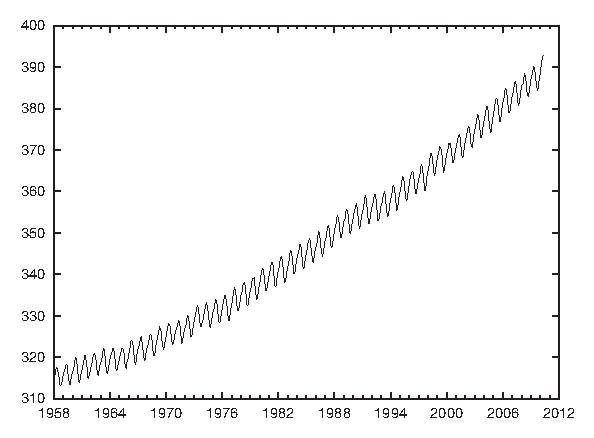
\includegraphics{img/co2hawaii}}
  \caption{Trend and seasonality: the concentration of CO$_2$
    (in parts per million) in the atmosphere as measured by the
    observatory on Mauna Loa, Hawaii, at monthly intervals.}
  \label{fig:co2hawaii}
\end{figure}

Figure \ref{fig:gasfurnace} displays the concentration of a certain
gas in the exhaust of a gas furnace over time. In many ways, this
example is the exact opposite of the previous example. Whereas the
data in Figure \ref{fig:co2hawaii} showed a lot of regularity and a
strong trend, the data in Figure \ref{fig:gasfurnace} shows no trend but
a lot of noise.

\begin{figure}
  \centerline{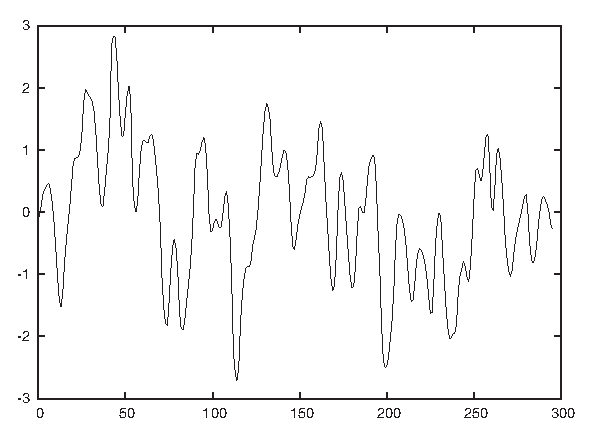
\includegraphics{img/gasfurnace}}
  \caption{No trend but relatively smooth variation over time:
    concentration of a certain gas in a furnace exhaust (in arbitrary
    units).}  
  \label{fig:gasfurnace}
\end{figure}

Figure \ref{fig:phonecost} shows the dramatic drop in the cost of a
typical long-distance phone call in the U.S.\ over the last century.
The strongly nonlinear trend is obviously the most outstanding feature
of this data set. As with many growth or decay processes, we may
suspect an exponential time development; in fact, in a
semi-logarithmic plot (Figure \ref{fig:phonecost}, inset) the data
follows almost a straight line, confirming our expectation. Any
analysis that fails to~account explicitly for this behavior of the
original data is likely to lead us astray. We should therefore work
with the logarithms of the cost, rather than with the absolute\break cost.

\begin{figure}
  \centerline{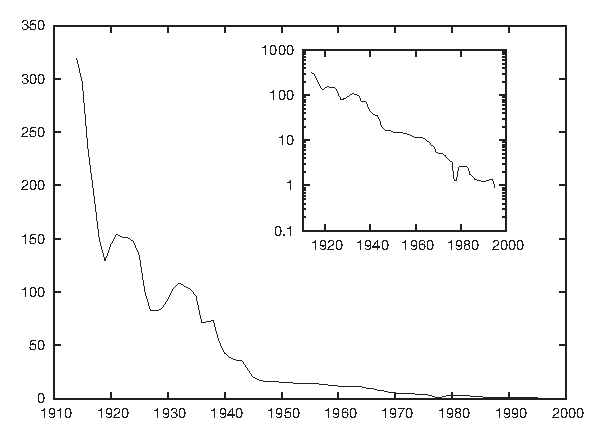
\includegraphics{img/phonecost}}
  \caption{Nonlinear trend: cost of a typical long-distance phone call
    in the U.S.}
  \label{fig:phonecost}
\end{figure}

There are some additional questions that we should ask when dealing
with a long-running data set like this.  What exactly is a ``typical''
long-distance call, and has that definition changed over the
observation period?  Are the costs adjusted for inflation or not? The
data itself also begs closer scrutiny. For instance, the
uncharacteristically low prices for a couple of years in the late
1970s make me suspicious: are they the result of a clerical error (a
typo), or are they real? Did the breakup of the AT\&T system\vadjust{\pagebreak} have
anything to do with these low prices? We will not follow up on these
questions here because I am presenting this example only as an
illustration of an exponential trend, but any serious analysis of this
data set would have to follow up on these questions.

\begin{figure}[t!]
   \centerline{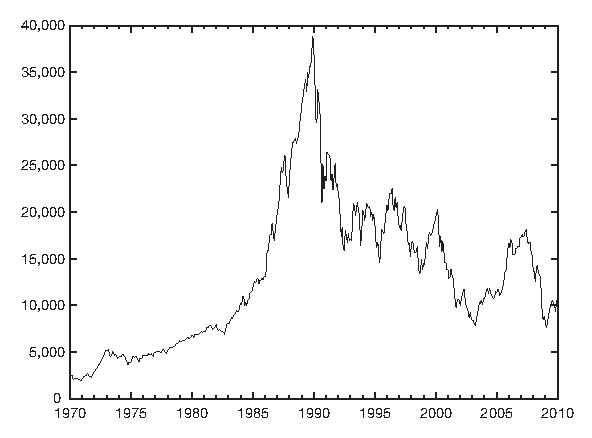
\includegraphics{img/nikkei}}
  \caption{Change in behavior: the Nikkei Stock Index over the last 
    40 years.}
  \label{fig:nikkei}
\end{figure}

Figure \ref{fig:nikkei} shows the development of the Japanese stock
market as represented by the Nikkei Stock Index over the last 40
years, an example of a time\vadjust{\pagebreak} series that exhibits a marked change in
behavior. Clearly, whatever was true before the New
Year's Day 1990 was no longer true afterward. (In fact, by looking
closely, you can make out a second change in behavior that was more
subtle than the bursting of the big Japanese bubble: its beginning,
sometime around 1985--1986.)

This data set should serve as a cautionary example. All time-series
analysis is based on the assumption that the processes generating the
data are stationary in time. If the rules of the game change, then
time-series analysis is the wrong tool for the task; instead we need
to investigate what caused the break in behavior. More benign examples
than the bursting of the Japanese bubble can be found: a change in
sales or advertising strategy may significantly alter a company's
sales patterns. In such cases, it is more important to inquire about
any further plans that the sales department might have, rather than to
continue working with data that is no longer representative!

After these examples that have been chosen for their ``textbook''
properties, let's look at a ``real-world'' data set. Figure
\ref{fig:callcenter} shows the number of daily calls placed to a call
center for a time period slightly longer than two years. In comparison
to the previous examples, this data set has a lot more structure,
which  makes it hard to determine even basic properties. We can see
some high-frequency variation, but it is not clear whether this is
noise or has some form of regularity to it. It is also not clear
whether there is any sort of regularity on a longer time scale.  The
amount of variation makes it hard to recognize any further structure.
For instance, we cannot tell if there is a longer-term trend in the
data. We will come back to this example later in the chapter.

\begin{figure}
  \centerline{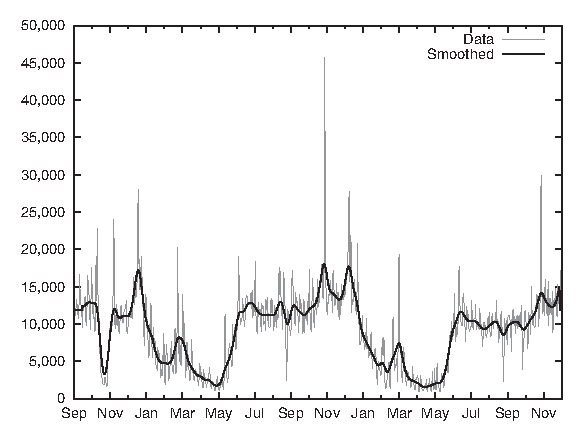
\includegraphics{img/callcenter}}
  \caption{A real-world data set: number of daily calls placed to a
    call center.  The data exhibits short- and long-term seasonality,
    noise, and possibly changes in behavior.  Also shown is the result
    of applying a 31-point Gaussian smoothing filter.}
  \label{fig:callcenter}
\end{figure}

\index{time-series analysis!examples|)} 

% ============================================================
\section{The Task}

\index{time-series analysis!components of|(} 

After this tour of possible time-series scenarios, we can identify the
main components of every time series:

\begin{itemize}
\item Trend\index{trends!time-series}
\item Seasonality\index{seasonality!time-series}
\item Noise\index{noise!time-series}
\item Other(!)
\end{itemize}

The trend may be linear or nonlinear, and we may want to investigate
its magnitude. The seasonality pattern may be either additive or
multiplicative. In the first case, the seasonal change has the same
\emph{absolute} size no matter what the magnitude of the current
baseline of the series is; in the latter case, the seasonal change has
the same \emph{relative} size compared with the current magnitude of
the series. Noise (\ie, some form of random variation) is almost
always part of a time series. Finding ways to reduce the noise in the
data is usually a significant part of the analysis process. Finally,
``other'' includes anything else that we may observe in a time series,
such as particular significant changes in overall behavior, special
outliers, missing data---anything remarkable at all.

Given this list of components, we can summarize what it means to
``analyze'' a time series. We can distinguish three basic tasks:

\begin{itemize}
\item Description
\item Prediction
\item Control
\end{itemize}

Description attempts to identify components of a time series (such as
trend and seasonality or abrupt changes in behavior). Prediction seeks
to forecast future values.  Control in this context means the
monitoring of a process over time with the purpose of keeping it
within a predefined band of values---a typical task in many
manufacturing or engineering environments. We can distinguish the
three tasks in terms of the time frame they address: description looks
into the past, prediction looks to the future, and control
concentrates on the present.\vspace*{-9pt}


\subsection{Requirements and the Real World}

Most standard methods of time-series analysis make a number of
assumptions about the underlying data.

\begin{itemize}
\item Data points have been taken at equally spaced time steps, with
  no missing data points.

\item The time series is sufficiently long (50 points are often 
  considered as an absolute minimum).

\item The series is \emph{stationary}: it has no trend, no
  seasonality, and the character (amplitude and frequency) of any
  noise does not change with time.
\end{itemize}

Unfortunately, most of these assumptions will be more or less violated
by any real-world data set that you are likely to encounter. Hence you
may have to perform a certain amount of data cleaning before you can
apply the methods described in this chapter.

If the data has been sampled at irregular time steps or if some of the
data points are missing, then you can try to interpolate the data and
resample it at equally spaced intervals. Time series obtained from
electrical systems or scientific experiments can be almost arbitrarily
long, but most series arising in a business context will be quite
short and contain possibly no more than two dozen data points. The
exponential smoothing methods introduced in the next section are
relatively robust even for relatively short series, but somewhere
there is a limit. Three or four data points don't constitute a series!
Finally, most interesting series will not be stationary in the sense
of the definition just given, so we may have to identify and remove
trend and seasonal components explicitly (we'll discuss how to do that
later). Drastic changes in the nature of the series also violate the
stationarity condition. In such cases we must not continue blindly but
instead deal with the break in the data---for example, by treating the
data set as two different series (one before and one after the event). 

\index{time-series analysis!components of|)} 

% ============================================================
\section{Smoothing}

\index{time-series analysis!smoothing|(}
\index{smoothing!time-series analysis|(}
  
An important aspect of most time series is, the presence of
\emph{noise}---that is, random (or apparently random) changes in the
quantity of\vadjust{\pagebreak} interest. Noise occurs in many real-world data sets, but
we can often reduce the noise by improving the apparatus used to
measure the data or by collecting a larger sample and averaging over
it. But the particular structure of time series makes this impossible:
the sales figures for the last 30 days are fixed, and they constitute
all the data we have. This means that removing noise, or at least
reducing its influence, is of particular importance in time-series
analysis. In other words, we are looking for ways to \emph{smooth} the
signal.


\begin{figure}
  \centerline{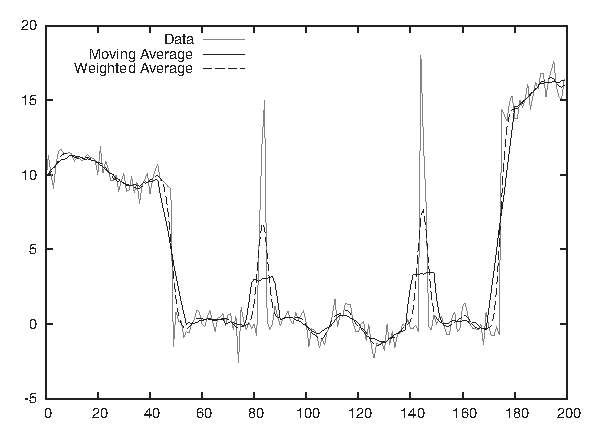
\includegraphics{img/runningavg}}
  \caption{Simple and a Gaussian weighted moving average: the weighted
    average is less affected by sudden jumps in the data.}
  \label{fig:runningavg}
\end{figure}

\subsection{Running Averages}

\index{running averages}
 
The simplest smoothing algorithm that we can devise is the
\emph{running}, \emph{moving}, or \emph{floating average}.\index{moving averages}\index{floating averages} The
idea is straightforward: for any odd number of consecutive points, replace the
centermost value with the average of the other points (here, the
$\braces{x_i}$ are the data points and the smoothed value at position
$i$ is $s_i$):
%
% x_i \rightarrow x_i = \frac{1}{2k+1} \sum_{j=-k}^k x_{i+j}
\[ 
s_i = \frac{1}{2k+1} \sum_{j=-k}^k x_{i+j}
\]
%
This naive approach has a serious problem, as you can see in Figure
\ref{fig:runningavg}. The figure shows the original signal together
with the 11-point moving average. Unfortunately, the signal has some
sudden jumps and occasional large ``spikes,'' and we can see how the
smoothed curve is affected by these events: whenever a spike enters
the smoothing window, the moving average is abruptly distorted by the
single, uncommonly large value until the outlier leaves the smoothing
window again---at which point the floating average equally abruptly
drops again.



We can avoid this problem by using a \emph{weighted moving average},\index{weighted moving averages} 
which places less weight on the points at the edge of the smoothing
window. Using such a weighted average, any new point that enters the
smoothing window is only gradually added to the average and then
gradually removed again:
%
% x_i \rightarrow x_i = \sum_{j=-k}^k w_j x_{i+j}
% \quad \text{ where } \sum_{j=-k}^k w_j = 1
\[ 
s_i = \sum_{j=-k}^k w_j x_{i+j} 
      \quad \text{where } \sum_{j=-k}^k w_j = 1
\]
%
Here the $w_j$ are the weighting factors. For example, for a 3-point
moving average, we might use $( 1/4, 1/2, 1/4 )$. The particular choice
of weight factors is not very important provided they are peaked at
the center, drop toward the edges, and add up to $1$. I like to use
the Gaussian function:\index{Gaussian distribution (Gaussian function)!moving averages}
%
\[ 
f(x,\sigma) = \frac{1}{\sqrt{2 \pi \sigma^2}} 
              \exp \paren{- \frac{1}{2} \paren{ \frac{x}{\sigma} }^2}
\]
%
to build smoothing weight factors. The parameter $\sigma$ in the
Gaussian controls the width of the curve, and the function is
essentially zero for values of $x$ larger than about $3.5 \sigma$.
Hence $f(x,1)$ can be used to build a 9-point kernel by evaluating
$f(x,1)$ at the positions $[-4,-3,-2,-1,0,1,2,3,4]$. Setting
$\sigma=2$, we can form a 15-point kernel by evaluating the Gaussian
for all integer arguments between $-7$ and $+7$. And so on.


\subsection{Exponential Smoothing}

\index{exponential smoothing|(}
 
All moving-average schemes have a number of problems.

\begin{itemize}
\item They are painful to evaluate. For each point, the calculation
  has to be performed from scratch. It is not possible to evaluate
  weighted moving averages by updating a previous result.

\item Moving averages can never be extended to the true edge of the
  available data set, because of the finite width of the averaging
  window. This is especially problematic because often it is precisely
  the behavior at the leading edge of a data set that we are most
  interested in.

\item Similarly, moving averages are not defined \emph{outside} the
  range of the existing data set.  As a consequence, they are of no
  use in forecasting.
\end{itemize}

Fortunately, there exists a very simple calculational scheme that
avoids all of these problems. It is called \emph{exponential
  smoothing} or \emph{Holt--Winters method}. There are various forms
of exponential smoothing: single exponential smoothing for series that
have neither trend nor seasonality, double exponential smoothing for
series exhibiting a trend but no seasonality, and triple exponential
smoothing for series with both trend and seasonality.  The term
``Holt--Winters method'' is sometimes reserved for triple exponential
smoothing alone.

All exponential smoothing methods work by updating the result from the
previous time step using the new information contained in the data of
the current time step. They do so by ``mixing'' the new information
with the old one, and the relative weight of old and new information
is controlled by an adjustable mixing parameter. The various methods
differ in terms of the number of quantities they track and the
corresponding number of mixing parameters.

The recurrence relation for single exponential smoothing is
particularly simple:
%
\[
s_i = \alpha x_i + (1-\alpha) s_{i-1} \quad \text{with $0 \le \alpha \le 1$}
\] 
%
Here $s_i$ is the smoothed value at time step $i$, and $x_i$ is the
actual (unsmoothed) data at that time step. You can see how $s_i$ is a
mixture of the raw data and the previous smoothed value $s_{i-1}$.
The mixing parameter $\alpha$ can be chosen anywhere between $0$ and
$1$, and it controls the balance between new and old information: as
$\alpha$ approaches $1$, we retain only the current data point (\ie,
the series is not smoothed at all); as $\alpha$ approaches $0$, we
retain only the smoothed past (\ie, the curve is totally flat).

Why is this method called ``exponential'' smoothing? To see this,
simply expand the recurrence relation:
%
\begin{align*}
  s_i & = \alpha x_i + ( 1 - \alpha ) s_{i-1} \\
      & = \alpha x_i + ( 1 - \alpha ) 
          \left[ \alpha x_{i-1} + ( 1 - \alpha ) s_{i-2} \right] \\
      & = \alpha x_i + ( 1 - \alpha ) 
          \bigl[ \alpha x_{i-1} + ( 1 - \alpha ) 
          \left[ \alpha x_{i-2} + ( 1 - \alpha ) s_{i-3} \right] \bigr] \\
      & = \alpha \left[ x_i + ( 1 - \alpha ) x_{i-1} + 
          ( 1 - \alpha )^2 x_{i-2} \right] + 
          ( 1 - \alpha )^3 s_{i-3} \\
      & = \dots \\
      & = \alpha \sum_{j=0}^{i} ( 1 - \alpha )^j x_{i-j}
\end{align*}
%
What this shows is that in exponential smoothing, \emph{all} previous
observations contribute to the smoothed value, but their contribution
is suppressed by increasing powers of the parameter $\alpha$.  That
observations further in the past are suppressed multiplicatively is
characteristic of exponential behavior.  In a way, exponential
smoothing is like a floating average with infinite memory but with
exponentially falling weights. (Also observe that the sum of the
weights, $\sum_j \alpha ( 1 - \alpha )^j$, equals $1$ as required by
virtue of the geometric series $\sum_i q^i = 1/(1-q)$ for $q < 1$. See
Appendix \ref{app:calculus} for information on the geometric series.)

The results of the simple exponential smoothing procedure can be
extended beyond the end of the data set and thereby used to make a
forecast. The forecast is extremely simple:
%
\[
x_{i+h} = s_i
\]
%
where $s_i$ is the last calculated value. In other words, single
exponential smoothing yields a forecast that is absolutely flat for
all times.

Single exponential smoothing as just described works well for time
series without an overall trend. However, in the presence of an
overall trend, the smoothed values tend to lag behind the raw data
unless $\alpha$ is chosen to be close to $1$; however, in this case
the resulting curve is not sufficiently smoothed.

Double exponential smoothing \index{double exponential smoothing} corrects for this shortcoming by
retaining explicit information about the trend. In other words, we
maintain and update the state of two quantities: the smoothed signal
\emph{and} the smoothed trend. There are two equations and two mixing
parameters:\vspace*{-6pt}
%
\begin{align*}
  s_i & = \alpha x_i + ( 1 - \alpha ) ( s_{i-1} + t_{i-1} ) \\
  t_i & = \beta ( s_i - s_{i-1} ) + ( 1 - \beta ) t_{i-1}
\end{align*}\vskip-3pt
%

\noindent Let's look at the second equation first. This equation describes the
smoothed trend. The current unsmoothed ``value'' of the trend is
calculated as the difference between the current and the previous
smoothed signal; in other words, the current trend tells us how much
the smoothed signal changed in the last step. To form the smoothed
trend, we perform a simple exponential smoothing process on the trend,
using the mixing parameter $\beta$. To obtain the smoothed signal, we
perform a similar mixing as before but consider not only the previous
smoothed signal but take the trend into account as well.  The last
term in the first equation is the best guess for the current smoothed
signal---assuming we followed the previous trend for a single time
step.

%\enlargethispage{6pt}

To turn this result into a forecast, we take the last smoothed value
and, for each additional time step, keep adding the last smoothed
trend to it:\vspace*{-3pt}
%
\[
x_{i+h} = s_i + h \, t_i
\]\vskip-6pt

Finally, for triple exponential smoothing \index{triple exponential smoothing} we add yet a third quantity,
which describes the seasonality. We have to distinguish between
additive and multiplicative seasonality. For the additive case, the
equations are:\vspace*{-3pt}
%
\begin{align*}
  s_i & = \alpha ( x_i - p_{i-k} ) + ( 1 - \alpha ) ( s_{i-1} + t_{i-1} ) \\
  t_i & = \beta ( s_i - s_{i-1} ) + ( 1 - \beta ) t_{i-1} \\
  p_i & = \gamma ( x_i - s_i ) + ( 1 - \gamma ) p_{i-k} \\
  x_{i+h} & = s_i + h \, t_i + p_{i-k+h}
\end{align*}
%
For the multiplicative case, they are:\vspace*{-3pt}
%
\begin{align*}
  s_i & = \alpha \frac{x_i}{p_{i-k}} + ( 1 - \alpha ) ( s_{i-1} + t_{i-1} ) \\
  t_i & = \beta ( s_i - s_{i-1} ) + ( 1 - \beta ) t_{i-1} \\
  p_i & = \gamma \frac{x_i}{s_i} + ( 1 - \gamma ) p_{i-k} \\
  x_{i+h} & = (s_i + h \, t_i) p_{i-k+h}
\end{align*}
%

\noindent Here, $p_i$ is the ``periodic'' component, and $k$ is the length of the
period. I have also included the expressions for forecasts.

All exponential smoothing methods are based on recurrence relations.\index{recurrence relations, exponential smoothing}
This means that we need to fix the start-up values in order to use
them.  Luckily, the specific choice for these values is not very
critical: the exponential damping implies that all exponential
smoothing methods have a short ``memory,'' so that after only a few
steps, any influence of the initial values is greatly diminished. Some
reasonable choices for start-up values are:
%
\[
s_0 = x_0  
\qquad \text{or} \qquad
s_0 = \frac{1}{n} \sum_i^n x_i \quad \text{with $1 < n < 5, \dots, 10$}
\]
%
and:
%
\[
t_0 = 0 
\qquad \text{or} \qquad
t_0 = x_1 - x_0
\]

For triple exponential smoothing we must provide one full season of
values for start-up, but we can simply fill them with $1$s (for the
multiplicative model) or $0$s (for the additive model). Only if the
series is short do we need to worry seriously about finding good
starting values.

The last question concerns how to choose the mixing parameters
$\alpha$, $\beta$, and $\gamma$. My advice is trial and error. Try a
few values between $0.2$ and $0.4$ (very roughly), and see what results
you get.  Alternatively, you can define a measure for the error
(between the actual data and the output of the smoothing algorithm),
and then use a numerical optimization routine to minimize this error
with respect to the parameters. In my experience, this is usually more
trouble than it's worth for at least the following two reasons. The
numerical optimization is an iterative process that is not guaranteed
to converge, and you may end up spending way too much time coaxing the
algorithm to convergence. Furthermore, any such numerical optimization
is slave to the expression you have chosen for the ``error'' to be
minimized. The problem is that the parameter values minimizing that
error may not have some other property you want to see in your
solution (\eg, regarding the balance between the accuracy of the
approximation and the smoothness of the resulting curve) so that, in
the end, the manual approach often comes out ahead. However, if you
have many series to forecast, then it may make sense to expend the
effort and build a system that can determine the optimal parameter
values automatically, but it probably won't be easy to really make
this work.

Finally, I want to present an example of the kind of results we can
expect from exponential smoothing. Figure \ref{fig:airtraffic} is a
classical data set that shows the monthly number of international
airline passengers (in thousands of passengers).\footnote{This data is
  available in the ``airpass.dat'' data set from R.\ J.\ Hyndman's
  Time Series Data Library at \url{http://www.robjhyndman.com/TSDL}.}
The graph shows the actual data together with a triple exponential
approximation. The years 1949 through 1957 were used to ``train'' the
algorithm, and the years 1958 through 1960 are forecasted.  Note how
well the forecast agrees with the actual data---especially in  
light of the strong seasonal pattern---for a rather long forecasting
time frame (three full years!). Not bad for a method as simple as
this.

\begin{figure}
  \centerline{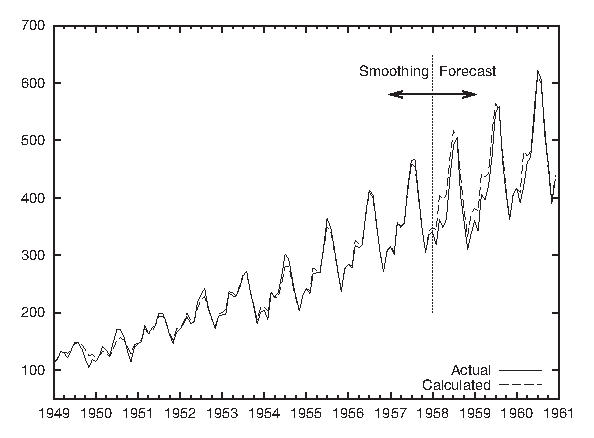
\includegraphics{img/airtraffic}}
  \caption{Triple exponential smoothing in action: comparison between
    the raw data (solid line) and the smoothed curve (dashed). For the
    years after 1957, the dashed curve shows the forecast calculated
    with only the data available in 1957.}
  \label{fig:airtraffic}
\end{figure}

\index{exponential smoothing|)}
\index{time-series analysis!smoothing|)}
\index{smoothing!time-series analysis|)}

\section{Don't Overlook the Obvious!}

On a recent consulting assignment, I was discussing monthly sales
numbers with the client when he made the following comment: ``Oh,
yes, sales for February are always somewhat lower---that's an
after effect of the Christmas peak.'' Sales are always lower in
\emph{February}? How interesting.

Sure enough, if you plotted the monthly sales numbers for the last few
years, there was a rather visible dip from the overall trend every
February. But in contrast, there wasn't much of a Christmas spike!
(The client's business was not particularly seasonal.) So why should
there be a corresponding dip two months later?

By now I am sure you know the answer already: February is
\emph{shorter} than any of the other months. And it's not a small
effect, either: with 28 days, February is about three days shorter than
the other months (which have 30--31 days). That's about 10
percent---close to the size of the dip in the client's sales numbers.

When monthly sales numbers were normalized by the number of days in
the month, the February dip all but disappeared, and the \emph{adjusted}
February numbers were perfectly in line with the rest of the months.
(The average number of days per month is $365/12 = 30.4$.)

Whenever you are tracking aggregated numbers in a time series (such as
weekly, monthly, or quarterly results), make sure that you have
adjusted for possible variation in the aggregation time frame. Besides
the numbers\vadjust{\pagebreak} of days in the month, another likely candidate for hiccups
is the number of \emph{business days} in a month (for months with five
weekends, you can expect a 20 percent drop for most business metrics).  But
the problem is, of course, much more general and can occur whenever you
are reporting aggregate \emph{numbers} rather than \emph{rates}. (If
the client had been reporting average sales per day for each month,
then there would never have been an anomaly.)

This specific problem (\ie, nonadjusted variations in aggregation
periods) is a particular concern for all business reports and
dashboards. Keep an eye out for it!


% ============================================================
\section{The Correlation Function}

\index{time-series analysis!correlation function|(} 
\index{correlation function|(}
 
The \emph{autocorrelation function} \index{autocorrelation function} is the primary diagnostic tool for
time-series analysis. Whereas the smoothing methods that we have
discussed so far deal with the raw data in a very direct way, the
correlation function provides us with a rather different view of the
same data. I will first explain how the autocorrelation function is
calculated and will then discuss what it means and how it can be used.

The basic algorithm works as follows: start with two copies of the
data set and subtract the overall average from all values.  Align the
two sets, and multiply the values at corresponding time steps with each
other. Sum up the results for all time steps. The result is the
(unnormalized) correlation coefficient at \emph{lag} $0$.  Now shift
the two copies against each other by a single time step.  Again
multiply and sum: the result is the correlation coefficient at lag
$1$. Proceed in this way for the entire length of the time series.
The set of all correlation coefficients for all lags is the
autocorrelation function. Finally, divide all coefficients by the
coefficient for lag $0$ to normalize the correlation function, so that
the coefficient for lag $0$ is now equal to $1$.

All this can be written compactly in a single formula for $c(k)$---that
is the correlation function at lag $k$:
%
\[
c(k) = \frac{\sum\limits_{i=1}^{N-k} (x_i - \mu)(x_{i+k} - \mu)}
            {\sum\limits_{i=1}^N (x_i - \mu)^2}
\qquad \text{with } \mu = \frac{1}{N} \sum_{i=1}^N x_i
\]
%
Here, $N$ is the number of points in the data set. The formula follows
the mathematical convention to start indexing sequences at $1$,
rather than the programming convention to start indexing at $0$.
Notice that we  have subtracted the overall average $\mu$ from all
values and that the denominator is simply the expression of the
numerator for lag $k=0$. Figure~\ref{fig:correlationlags} illustrates
the process.


\begin{figure}
 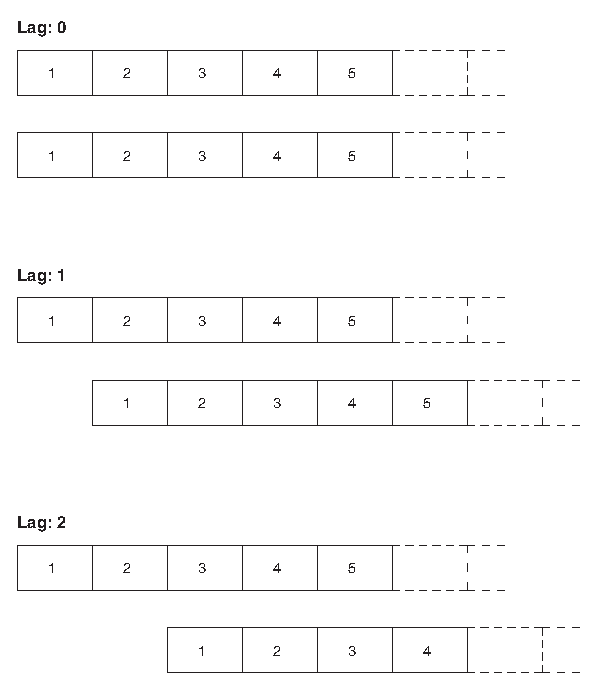
\includegraphics[scale=0.8]{img/correlationlags}
 \caption{Algorithm to compute the correlation function.}
 \label{fig:correlationlags}\vspace*{15pt}
\end{figure}

The meaning of the correlation function should be clear. Initially,
the two signals are perfectly aligned and the correlation is $1$.
Then, as we shift the signals against each other, they slowly move out
of phase with each\vadjust{\pagebreak} other, and the correlation drops. How quickly it
drops tells us how much ``memory'' there is in the data. If the
correlation drops quickly, we know that, after a few steps, the signal
has lost all memory of its recent past. However, if the correlation
drops slowly, then we know that we are dealing with a process that is
relatively steady over longer periods of time. It is also possible
that the correlation function first drops and then rises again to form
a second (and possibly a third, or fourth$,\dots$) peak. This tells us
that the two signals align again if we shift them far enough---in
other words, that there is periodicity (\ie, seasonality) in the data
set. The position of the secondary peak gives us the number of time
steps per season.

\vspace*{6pt}
\subsection{Examples}
Let's look at a couple of examples. Figure \ref{fig:gasfurnacecorr}
shows the correlation function of the gas furnace data in Figure
\ref{fig:gasfurnace}. This is a fairly typical correlation function
for a time series that has only short time correlations: the
correlation falls quickly, but not immediately, to zero. There is no
periodicity; after the initial drop, the correlation function does not
exhibit any further significant\vadjust{\vfill\pagebreak} peaks.





\begin{figure}
    \centerline{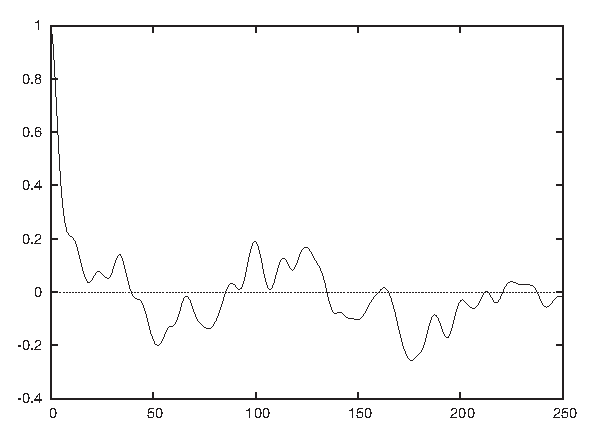
\includegraphics{img/gasfurnacecorr}}
  \caption{The correlation function for the exhaust gas data shown in
    Figure \ref{fig:gasfurnace}. The data has only short time
    correlations and no seasonality; the correlation function falls
    quickly (but not immediately) to zero, and there are no secondary
    peaks.}
  \label{fig:gasfurnacecorr}
\end{figure}

Figure \ref{fig:callcentercorr} is the correlation function for the
call center data from Figure \ref{fig:callcenter}. This data set shows
a very different behavior. First of all, the time series has a much
longer ``memory'': it takes the correlation function almost 100 days
to fall to zero, indicating that the frequency of calls to the call
center changes more or less once per quarter but not more frequently.
The second notable feature is the pronounced secondary peak at a lag
of 365 days. In other words, the call center data is highly seasonal
and repeats itself on a yearly basis.  The third feature is the small
but regular sawtooth structure. If we look closely, we will find that
the first peak of the sawtooth is at a lag of 7 days and that all
repeating ones occur at multiples of 7. This is the signature of the
high-frequency component that we could see in Figure
\ref{fig:callcenter}: the traffic to the call center exhibits a
secondary seasonal component with 7-day periodicity. In other words,
traffic is weekday dependent (which is not too surprising).

\begin{figure}
  \centerline{ 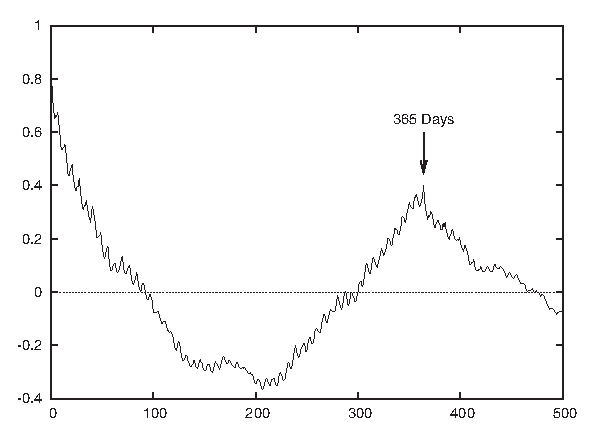
\includegraphics{img/callcentercorr}}
  \caption{The correlation function for the call center data shown in
    Figure \ref{fig:callcenter}. There is a secondary peak after
    exactly 365 days, as well as a smaller weekly structure to the
    data.}
  \label{fig:callcentercorr}
\end{figure}


\subsection{Implementation Issues}

So far I have talked about the correlation function mostly from a
conceptual point of view. If we want to proceed to an actual
implementation, there are some fine points we need to worry about.

The autocorrelation function \index{autocorrelation function} is intended for time series that do not
exhibit a trend \index{trends!time-series} and have zero mean. Therefore, if the series we want
to analyze does contain a trend, then we must remove it first. There
are two ways to do this: we can either subtract the trend or we can
difference the series.

Subtracting the trend is straightforward---the only problem is that we
need to determine the trend first! Sometimes we may have a ``model''
for the expected behavior and can use it to construct an explicit
expression for the trend.  For instance, the airline passenger data
from the previous section, describes a growth process, and so we should
suspect an exponential trend ($a \exp(x/b)$).  We can now try guessing
values for the two parameters and then subtract the exponential term
from the data. For other data sets, we might try a linear or power-law
trend, depending on the data set and our understanding of the process
generating the data. Alternatively, we might first apply a smoothing
algorithm to the data and then subtract the result of the smoothing
process from the raw data. The result will be the trend-free ``noise''
component of the time series.

A different approach consists of \emph{differencing} \index{differencing, time-series} the series:
instead of dealing with the raw data, we instead work with the
\emph{changes} in the data from one time step to the next.
Technically, this means replacing the original series $x_i$ with one
consisting of the differences of consecutive elements: $x_{i+1} -
x_i$. This process can be repeated if necessary, but in most cases,
single differencing is sufficient to remove the trend entirely.

Making sure that the time series has zero mean is easier: simply
calculate the mean of the (de-trended!) series and subtract it before
calculating the correlation function.  This is done explicitly in the
formula for the correlation function  given earlier.

Another technical wrinkle concerns how we implement the sum in the
formula for the numerator. As written, this sum is slightly messy,
because its upper limit depends on the lag.  We can simplify the
formula by \emph{padding} one of the data sets with $N$ zeros on the
right and letting the sum run from $i=1$ to $i=N$ for all\vadjust{\pagebreak} lags. In
fact, many computational software packages assume that the data has
been prepared in this way (see the Workshop section in this chapter).

The last issue you should be aware of is that there are two different
normalization conventions for the autocorrelation function, which are
both widely used. In the first variant, numerator and denominator are
not normalized separately---this is the scheme used in the previous
formula.  In the second variant, the numerator and denominator are
each normalized by the number of nonzero terms in their respective
sum.  With this convention, the formula becomes:
%
\[
c(k) = \frac{ \dfrac{1}{N-k} \sum\limits_{i=1}^{N-k} 
                                        (x_i - \mu)(x_{i+k} - \mu) }
            { \dfrac{1}{N} \sum\limits_{i=1}^N (x_i - \mu)^2 }
       \qquad \text{with } \mu = \frac{1}{N} \sum_{i=1}^N x_i
\]
%
Both conventions are fine, but if you want to compare results from
different sources or different software packages, then you will have
to make sure you know which convention each of them is following!\vspace*{-9pt}

\index{time-series analysis!correlation function|)} 
\index{correlation function|)}

% ============================================================
\section{Optional: Filters and Convolutions}

\index{time-series analysis!filters and convolutions}
\index{filters, time-series analysis}
\index{convolutions, time-series analysis}  
 
Until now we have always spoken of time series in a direct fashion,
but there is also a way to describe them (and the operations performed
on them) on a much higher level of abstraction. For this, we borrow
some concepts and terminology from electrical engineering,
specifically from the field of digital signal processing (DSP).\index{DSP (digital signal processing)} \index{digital signal processing (DSP)} 

In the lingo of DSP, we deal with \emph{signals} (time series)\index{signals, DSP} and
\emph{filters} (operations). Applying a filter to a signal produces a
new (filtered) signal. Since filters can be applied to any signal, we
can apply another filter to the output of the first and in this way
chain filters together (see Figure \ref{fig:filterchain}).  Signals
can also be combined and subtracted from each other.

\begin{figure}
  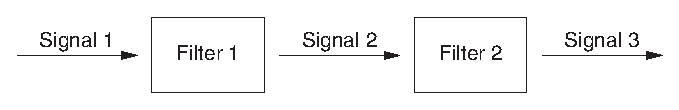
\includegraphics{img/filterchain}
  \caption{A filter chain: each filter applied to a signal yields another
    signal, which itself can be filtered.}
  \label{fig:filterchain}\vspace*{-9pt}
\end{figure} 

As it turns out, many of the operations we have seen so far
(smoothing, differencing) can be expressed as filters. We can
therefore use the convenient high-level language of DSP when
referring to the processes of time-series analysis. To make this
concrete, we need to understand how a filter is represented and what
it means to ``apply'' a filter to a signal.

Each digital filter is represented by a set of coefficients or
weights. To apply the filter, we multiply the coefficients with a subset
of the signal. The sum of the products is the value of the resulting
(filtered) signal:
%
\[
y_t = \sum_{i=-k}^k w_i x_{t+i}
\]
%
\clearpage

\noindent
This should look familiar! We used a similar expression when talking
about moving averages earlier in the chapter. A moving average is
simply a time series run through an $n$-point filter, where every
coefficient is equal to $1/n$. A weighted moving average filter
similarly consists of the weights used in the expression for the
average.

The filter concept is not limited to smoothing operations. The
differencing step discussed in the previous section can be viewed as
the application of the filter $[1, -1]$. We can even shift an entire
time series forward in time by using the filter $[0, 1]$.

The last piece of terminology that we will need concerns the peculiar
sum of a product that we have encountered several times by now.  It's
called a \emph{convolution}. A convolution is a way to combine two
sequences to yield a third sequence, which you can think of as
the ``overlap'' between the original sequences. The convolution
operation is usually defined as follows:
%
\[
y_t = \sum_{i=-\infty}^\infty w_i x_{t-i}
\]
%
Symbolically, the convolution operation is often expressed through an
asterisk: $y = w \star x$, where $y$, $w$, and $x$ are sequences.

Of course, if one or both of the sequences have only a finite number
of elements, then the sum also contains only a finite number of terms
and therefore poses no difficulties. You should be able to convince
yourself that every application of a filter to a time series that we
have done was in fact a convolution of the signal with the filter.
This is true in general: applying a filter to a signal means forming
the convolution of the two. You will find that many numerical software
packages provide a convolution operation as a built-in function,
making filter operations particularly convenient to use.

I must warn you, however, that the entire machinery of digital signal
processing is geared toward signals of infinite (or almost infinite)
length, which makes good sense for typical electrical signals (such as
the output from a microphone or a radio receiver). But for the rather
short time series that we are likely to deal with, we need to pay
close attention to a variety of \emph{edge effects}.  For example, if
we apply a smoothing or differencing filter, then the resulting series
will be shorter, by half the filter length, than the original series.
If we now want to subtract the smoothed from the original signal, the
operation will fail because the two signals are not of equal length.
We therefore must either pad the smoothed signal or truncate the
original one. The constant need to worry about padding and proper
alignment detracts significantly from the conceptual beauty of the
signal-theoretic approach when used with time series of relatively
short duration. 

% ============================================================
\section{Workshop: scipy.signal}

\index{time-series analysis!scipy.signal|(}
\index{scipy.signal|(}  

The \texttt{scipy.signal} package provides functions and operations
for digital signal processing that we can use to good effect to
perform calculations\vadjust{\pagebreak} for time-series analysis. The
\texttt{scipy.signal} package makes use of the signal processing
terminology introduced in the previous section.

The listing that follows shows all the commands used to create graphs
like Figures \ref{fig:callcenter} and \ref{fig:callcentercorr},
including the commands required to write the results to file. The code
is heavily commented and should be easy to understand.

\begin{verbatim}
from scipy import *
from scipy.signal import *
from matplotlib.pyplot import *

filename = 'callcenter'


# Read data from a text file, retaining only the third column.
# (Column indexes start at 0.)
# The default delimiter is any whitespace.
data = loadtxt( filename, comments='#', delimiter=None, usecols=(2,) )

# The number of points in the time series. We will need it later.
n = data.shape[0]

# Finding a smoothed version of the time series:
# 1) Construct a 31-point Gaussian filter with standard deviation = 4
filt = gaussian( 31, 4 )
# 2) Normalize the filter through dividing by the sum of its elements
filt /= sum( filt )
# 3) Pad data on both sides with half the filter length of the last value
#    (The function ones(k) returns a vector of length k, with all elements 1.)
padded = concatenate( (data[0]*ones(31//2), data, data[n-1]*ones(31//2)) )
# 4) Convolve the data with the filter. See text for the meaning of "mode".
smooth = convolve( padded, filt, mode='valid' )

# Plot the raw data together with the smoothed data:
# 1) Create a figure, sized to 7x5 inches
figure( 1, figsize=( 7, 5 ) )
# 2) Plot the raw data in red
plot( data, 'r' )
# 3) Plot the smoothed data in blue
plot( smooth, 'b' )
# 4) Save the figure to file
savefig( filename + "_smooth.png" )
# 5) Clear the figure
clf()

# Calculate the autocorrelation function:
# 1) Subtract the mean 
tmp = data - mean(data)
# 2) Pad one copy of data on the right with zeros, then form correlation fct
#    The function zeros_like(v) creates a vector with the same dimensions
#    as the input vector v but with all elements zero.
corr = correlate( tmp, concatenate( (tmp, zeros_like(tmp)) ), mode='valid' )
# 3) Retain only some of the elements
corr = corr[:500]
\end{verbatim}
\begin{verbatim}
# 4) Normalize by dividing by the first element
corr /= corr[0]


# Plot the correlation function:
figure( 2, figsize=( 7, 5 ) )
plot( corr )
savefig( filename + "_corr.png" )
clf()
\end{verbatim}

The package provides the Gaussian filter as well as many others.  The
filters are not normalized, but this is easy enough to accomplish.

More attention needs to be paid to the appropriate padding and
truncating. For example, when forming the smoothed version of the
data, I pad the data on both sides by half the filter length to ensure
that the smoothed data has the same length as the original set. The
\texttt{mode} argument to the \texttt{convolve()} and
\texttt{correlate} functions determines which pieces of the resulting
vector to retain. Several modes are possible. With
\texttt{mode="same"}, the returned vector has as many elements as the
largest input vector (in our case, as the padded data vector), but the
elements closest to the ends would be corrupted by the padded values.
In the listing, I therefore use \texttt{mode="valid"}, which retains
only those elements that have full overlap between the data and the
filter---in effect, removing the elements added in the padding step.

Notice how the signal processing machinery leads in this application
to very compact code. Once you strip out the comments and plotting
commands, there are only about 10 lines of code that perform actual
operations  and calculations.  However, we had to pad all data
carefully and ensure that we kept only those pieces of the result that
were least contaminated by the padding.

\index{time-series analysis!scipy.signal|)}
\index{scipy.signal|)}  

% ============================================================
% \section{Summary}
% 
% Time series are both common and important. But because they arise in
% so many, and so many \emph{different} contexts, little can be said
% about them without knowing the details. Studying and classifying the
% nature of each time series is therefore very important --- blindly
% applying ``cook book'' methods, no matter how sophisticated, is never
% a good strategy.
% 
% The two most important tools for studying time series are the time
% plot and the plot of the auto-correlation function. Both together can
% reveal most of what can be found out about any particular time series.
% The signal theoretic methodology that we discussed briefly can provide
% a convenient framework to handle the calculations that are required.
% 
% Smoothing and forecasting are the two most often desired results of
% time series analysis and here I strongly recommend simple, yet robust
% methods, such as weighted averages (for smoothing) and exponential
% smoothing (for forecasting).

% ============================================================
\section{Further Reading}

\begin{itemize}
\item \cit{The Analysis of Time Series}{Chris Chatfield}{6th ed.,
    Chapman \& Hall}{2003}
    This is my preferred text on time-series analysis. It combines a
    thoroughly practical approach with mathematical depth and a healthy
    preference for the simple over the obscure. Highly recommended.
\end{itemize}

\index{time-series analysis|)} 
\index{data analysis!time-series analysis|)}
 % done

% Mikes: ok
% Spellcheck: ok

% ============================================================
\chapter{More Than Two Variables: Graphical Multivariate Analysis}{}{}
\label{ch:multivariate}

\index{data analysis!multivariate analysis|(} 
\index{multivariate analysis|(} 

\Fint{As soon as we are dealing with more than two variables
simultaneously, things become much more} complicated---in particular,
graphical methods quickly become impractical. In this chapter, I'll
introduce a number of graphical methods that can be applied to
multivariate problems. All of them work best if the number of variables
is not \emph{too} large (less than 15--25).

The borderline case of \emph{three} variables can be handled through
\emph{false-color plots}, which we will discuss first.

If the number of variables is greater (but not much greater) than
three, then we can construct multiplots from a collection of
individual bivariate plots by scanning through the various parameters
in a systematic way. This gives rise to scatter-plot matrices and
co-plots.

Depicting how an overall entity is composed out of its constituent
parts can be a rather nasty problem, especially if the composition
changes over time. Because this task is so common, I'll treat it
separately in its own section.

Multi-dimensional visualization continues to be a research topic, and in
the last sections of the chapter, we look at some of the more recent
ideas in this field.

One recurring theme in this chapter is the need for adequate tools:
most multi-\break dimensional visualization techniques are either not
practical with paper and pencil, or are outright impossible without a
computer (in particular when it comes to animated techniques).
Moreover, as the number of variables increases, so does the need to
look at a data set from different angles; this leads to the idea of
using interactive graphics for exploration. In the last section, we
look at some ideas in this area.

% ============================================================
\section{False-Color Plots}

\index{multivariate analysis!false-color plots|(} 
\index{false-color plots|(}
\index{color, false-color plots|(}

There are different ways to display information in three variables
(typically, two independent variables and one dependent variable).
Keep in mind that simple is sometimes best! Figure \ref{fig:landau}
shows the function $f(x,a) = x^4/2 + a x^2 - x/2 + a/4$ for various
values of the parameter $a$ in a simple, two-dimensional $xy$ plot.
The shape of the function and the way it changes with $a$ are
perfectly clear in this graph. It is very difficult to display this
function in any other way with comparable clarity.

\begin{figure}
   \centerline{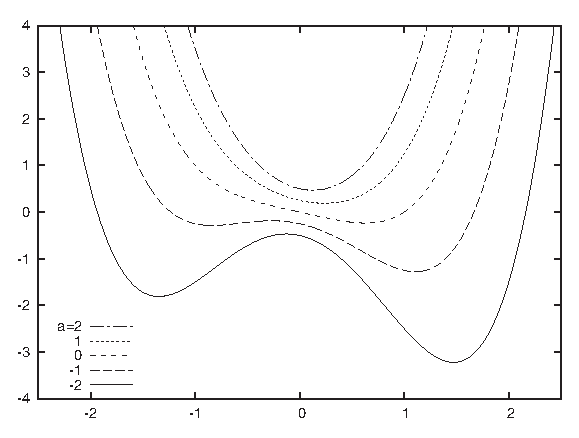
\includegraphics{img/landau}}
  \caption{A simple but effective way to show three variables: treat 
    one as parameter and draw a separate curve for several parameter
    values.}
  \label{fig:landau}\vspace*{12pt}
\end{figure}

Another way to represent such trivariate data is in the form of a
\emph{surface plot}, \index{surface plots} such as the one shown in Figure
\ref{fig:surface}.  As a rule, surface plots are visually stunning but
are of very limited practical utility. Unless the data set is very
smooth and allows for a viewpoint such that we can look \emph{down}
onto the surface, they simply don't work! For example, it is pretty
much impossible to develop a good sense for the behavior of the
function plotted in Figure \ref{fig:landau} from a surface plot. (Try
it!)  Surface plots can help build intuition for the overall
structure of the data, but it is notoriously difficult to read off
quantitative information from them.

\begin{figure}
    \centerline{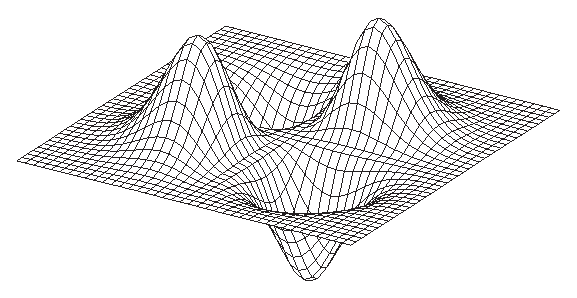
\includegraphics{img/surface}}
  \caption{Surface plots are often visually impressive but generally
    don't represent quantitative information very well.}
  \label{fig:surface}
\end{figure}

In my opinion, surface plots have only two uses:
\begin{enumerate}
\item To get an intuitive impression of the ``lay of the land'' for
  a complicated data set
\item To dazzle the boss (not that this isn't important at times)\vfill\pagebreak
\end{enumerate}

Another approach is to project the function into the base plane below
the surface in Figure \ref{fig:surface}. There are two ways in which
we can represent values: either by showing contours of constant
alleviation in a \emph{contour plot} \index{contour plots} or by mapping the numerical
values to a palette of colors in a \emph{false-color plot}. Contour
plots are familiar from topographic maps---they can work quite well,
in particular if the data is relatively smooth and if one is primarily
interested in local properties.

The false-color plot is an alternative and quite versatile technique
that can be used for different tasks and on a wide variety of data
sets. To create a false-color plot, all values of the dependent
variable $z$ are mapped to a palette of colors. Each data point is
then plotted as a region of the appropriate color. Figure
\ref{fig:grayscale} gives an example (where the color has been
replaced by grayscale shading).

\begin{figure}
   \centerline{\includegraphics{img/falsecolor}}
  \caption{Grayscale version of a false-color plot of the function
    shown as a surface plot in Figure \ref{fig:surface}.  Here white
    corresponds to positive values of the function, and black
    corresponds to negative values.}
  \label{fig:grayscale}
\end{figure}\pagebreak

I like false-color plots because one can represent a lot of
information in a them in a way that retains quantitative information.
However, false-color plots depend crucially on the quality of the
palette---that is, the mapping that has been used to associate colors
with numeric values.

Let's quickly recap some information on color and computer graphics.
Colors for computer graphics are usually specified by a triple of
numbers that specify the intensity of their red, green, and blue (RGB)
components. Although RGB triples make good sense technically, they are
not particularly intuitive. Instead, we tend to think of color in
terms of its hue, saturation, and value (\ie, luminance  or lightness).
Conventionally, hue runs through all the colors of the rainbow (from
red to yellow, green, blue, and magenta). Curiously, the spectrum of
hues seems to circle back onto itself, since magenta smoothly transforms
back to red. (The reason for this behavior is that the hues in the
rainbow spectrum are arranged in order of their dominant
electromagnetic frequency. For violet/magenta, no frequency dominates;
instead, violet is a mixture of low-frequency reds and high-frequency
blues.) Most computer graphics programs will be able to generate color
graphics using a hue--saturation--value (HSV) triple.

It is surprisingly hard to find reliable recommendations on good
palette design, which is even more unfortunate given that convenience
and what seems like common sense often lead to particularly \emph{bad}
palettes. Here are some ideas and suggestions that you may wish to
consider:
\begin{unnumlist}
\subparagraph{Keep it simple}
\item Very simple palettes using red, white, and blue
  often work surprisingly well. For continuous color changes you could
  use a blue-white-red palette, for segmentation tasks you could use
  a white-blue-red-white palette with a sharp blue--red transition
  at the segmentation threshold.

\subparagraph{Distinguish between segmentation tasks and the display of smooth
  changes}
\item Segmentation tasks (\eg, finding all points that exceed a
  certain threshold, finding the locations where the data crosses
  zero) call for palettes with sharp color transitions at the
  respective thresholds, whereas representing smooth changes in a data
  set calls for continuous color gradients. Of course, both aspects
  can be combined in a single palette: gradients for part of the
  palette and sharp transitions elsewhere.

\subparagraph{Try to maintain an intuitive sense of ordering}
\item Map low values
  to ``cold'' colors and higher values to ``hot'' colors to provide an
  intuitive sense of ordering in your palette. Examples include the
  simple blue-red palette and the ``heat scale'' 
  (black-red-yellow-white---I'll discuss in a moment why I don't
  recommend the heat scale for use). Other palettes that convey a
  sense of ordering (if only by convention) are the ``improved
  rainbow'' (blue-cyan-green-\break yellow-orange-red-magenta) and the
  ``geo-scale'' familiar from topographic maps
  (blue-cyan-green-brown-tan-white).\pagebreak

\subparagraph{Place strong visual gradients in regions with important changes}
\item
  Suppose that you have a data set with values that span the range
  from $-100$ to $+100$ but that all the really interesting or
  important change occurs in the range $-10$ to $+10$. If you use a
  standard palette (such as the improved rainbow) for such a data set,
  then the actual region of interest will appear to be all of the same
  color, and the rest of the spectrum will be ``wasted'' on parts of
  the data range that are not that interesting.  To avoid this
  outcome, you have to compress the rainbow so that it maps only to
  the region of interest. You might want to consider mapping the
  extreme values (from $-100$ to $-10$ and from $10$ to $100$) to some
  unobtrusive colors (possibly even to a grayscale) and reserving the
  majority of hue changes for the most relevant part of the data
  range.

\subparagraph{Favor subtle changes}
\item This is possibly the most surprising
  recommendation. When creating palettes, there is a natural tendency
  to ``crank it up full'' by using fully saturated colors at maximal
  brightness throughout. That's not necessarily a good idea, because
  the resulting effect can be so harsh that details are easily lost.
  Instead, you might want to consider using soft, pastel colors or
  even to experiment with mixed hues in favor of the pure primaries of
  the standard rainbow. (Recent versions of Microsoft Excel provide an
  interesting and easily accessible demonstration for this idea: all
  default colors offered for shading the background of cells are soft,
  mixed pastels---to good effect.)  Furthermore, the eye is quite
  good at detecting even subtle variations.  In particular, when
  working with luminance-based palettes, small changes are often all
  that is required.

\subparagraph{Avoid changes that are hard to detect}
\item Some visual changes are
  especially hard to perceive visually. For example, it is practically
  impossible to distinguish between different shades of yellow, and
  the transition from yellow to white is even worse!  (This is why I
  don't recommend the heat scale, despite its nice ordering property:
  the bottom third consists of hard-to-distinguish dark reds, and the
  entire upper third consists of very hard-to-distinguish shades of
  light yellow.)

\subparagraph{Use hue- and luminance-based palettes for different purposes}
\item In
  particular, consider using a luminance-based palette to emphasize
  fine detail and using hue- or saturation-based palettes for smooth,
  large-scale changes. There is some empirical evidence that
  luminance-based palettes are better suited for images that contain a
  lot of fine detail and that hue-based palettes are better suited for
  bringing out smooth, global changes. A pretty striking demonstration
  of this observation can be found when looking at medical images
  (surely an application where details matter!): a simple grayscale
  representation, which is pure luminance, often seems much clearer
  than a multicolored representation using a hue-based rainbow
  palette.  This rule is more relevant\vadjust{\pagebreak} to image processing of
  photographs or similar images (such as that in our medical example)
  than to visualization of the sort of abstract information that we
  consider here, but it is worth keeping in mind.
  
\subparagraph{Don't forget to provide a color box}
\item No matter how intuitive you
  think your palette is, nobody will know for sure what you are
  showing unless you provide a color box (or color key) that shows the
  values and the colors they are mapped to.  Always, always, provide
  one.
\end{unnumlist}

One big problem not properly addressed by these recommendations
concerns \emph{visual uniformity}. \index{visual uniformity} For example, consider palettes
based on the ``improved rainbow,'' which is created by distributing
the six primaries in the order blue-cyan-green-yellow-red-magenta
across the palette. If you place these primaries at equal distances
across from each other and interpolate linearly between them in color
space, then the fraction of the palette occupied by green appears to
be much larger than the fraction occupied by either yellow or cyan.
Another example is that when placing a fully saturated yellow next to
a fully saturated blue, then the blue region will appear to be more
intense (\ie, saturated) than the yellow. Similarly, the browns that
occur in a geo-scale easily appear darker than the other colors in the
palette. This is a problem with our \emph{perception} of color: simple
interpolations in color space do not necessarily result in visually
uniform gradients!

There is a variation of the HSV color space, called the \emph{HCL}
(hue--chroma--luminance) space \index{HCL (hue--chroma--luminance) space} that takes visual perception into
account to generate visually uniform color maps and gradients.  The
HCL color model is more complicated to use than the HSV model, because
not all combinations of hue, chroma, and luminance values exist.  For
instance, a fully saturated yellow appears lighter than a fully
saturated blue, so a palette at full chroma and with high luminance
will include the fully saturated yellow but not the blue. As a result,
HCL-based palettes that span the entire rainbow of hues tend naturally
toward soft, pastel colors.  A disadvantage of palettes in the HCL
space is that they often degrade particularly poorly when reproduced
in black and white.\footnote{An implementation of the transformations
  between HCL and RGB is available in R and C in the ``colorspace''
  module available from CRAN.}

A special case of false-color plots are geographic \emph{maps}, and
cartographers have significant experience developing color schemes for
various purposes. Their needs are a little different and not all of
their recommendations may work for general data analysis purposes, but
it is worthwhile to become familiar with what they have
learned.\footnote{An interesting starting point is Cynthia Brewer's
  online ColorBrewer at \url{http://colorbrewer2.org/}.}

Finally, I'd like to point out two additional problems with all
plots that depend on color to convey critical information.

\begin{itemize}
\item Color does not reproduce well. Once photocopied or printed on a
  black-and-white laser printer, a false-color plot will become
  useless!
\item Also keep in mind that about 10 percent of all men are at least
  partially color blind; these individuals won't be able to make much
  sense of most images that rely heavily or exclusively on color.
\end{itemize}

Either one of these problems is potentially serious enough that you
might want to reconsider before relying entirely on color for the
display of information.

In my experience, preparing good false-color plots is often a tedious
and time-consuming task. This is one area where better tools would be
highly desirable---an interactive tool that could be used to
manipulate palettes directly and in real time would be very nice to
have. The same is true for a publicly available set of well-tested
palettes.

\index{multivariate analysis!false-color plots|)} 
\index{false-color plots|)}
\index{color, false-color plots|)}

% ============================================================
\section{A Lot at a Glance: Multiplots}

\index{multivariate analysis!multiplots|(} 
\index{multiplots|(} 

The primary concern in all multivariate visualizations is finding
better ways to put more ``stuff'' on a graph. In addition to color
(see the previous section), there are basically two ways we can go
about this. We can make the graph elements themselves richer, so that
they can convey additional information beyond their position on the
graph; or we can put several similar graphs next to each other and
vary the variables that are not explicitly displayed in a systematic
fashion from one subgraph to the next. The first idea leads to
\emph{glyphs}, which we will introduce later in this chapter, whereas
the latter idea leads to scatter-plot matrices and co-plots.

\subsection{The Scatter-Plot Matrix}

\index{multiplots!scatter-plot matrices|(} 
\index{scatter-plot matrices|(} 

For a \emph{scatter-plot matrix} (occasionally abbreviated SPLOM), we
construct all possible two-dimensional scatter plots from a
multivariate data set and then plot them together in a matrix format
(Figure \ref{fig:splom}). We can now scan all of the graphs for
interesting behavior, such as a marked correlation between any two
variables.

\begin{figure}
  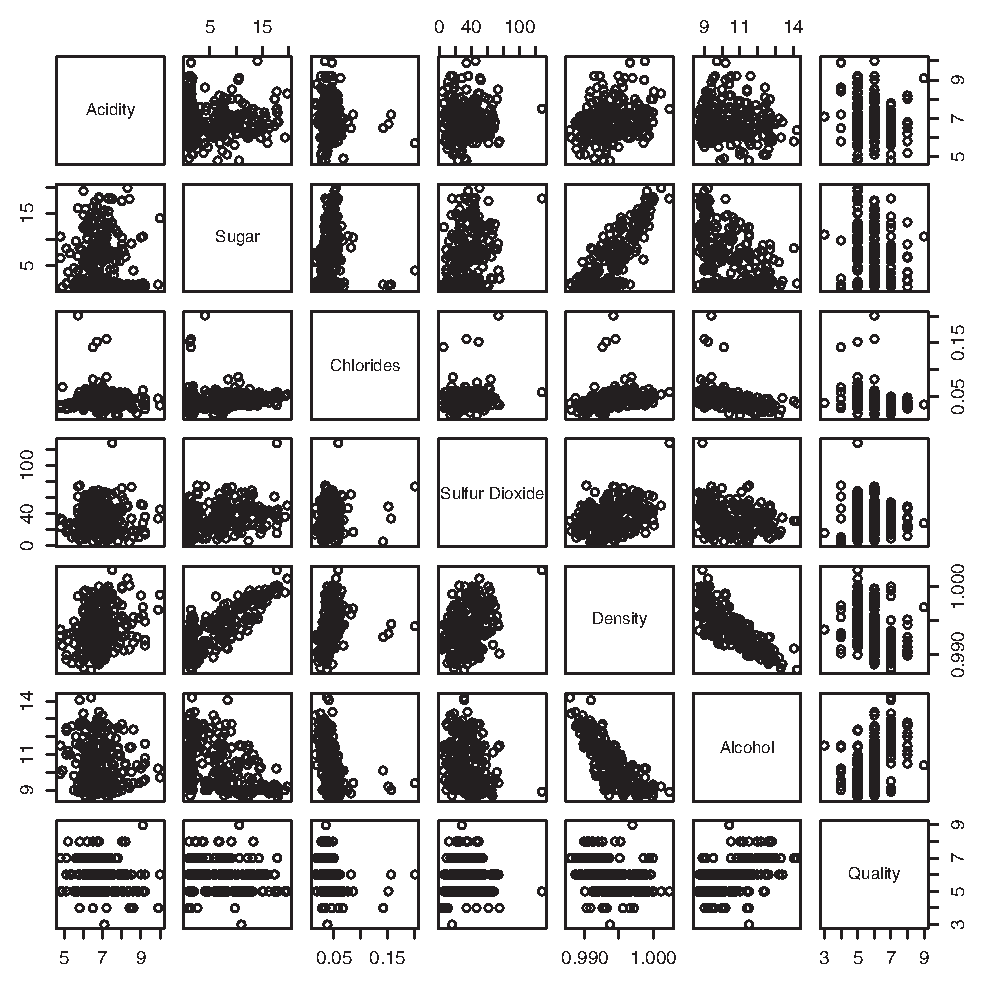
\includegraphics[width=\textwidth]{img/splom.eps}
  \caption{In a scatter-plot matrix (SPLOM), a separate scatter plot is
    shown for each pair of variables. All scatter plots in a given row
    or column have the same plot range, so that we can compare them
    easily.}
  \label{fig:splom}\vspace*{-6pt}
\end{figure}

The data set shown in Figure \ref{fig:splom} consists of seven
different properties of a sample of 250 wines.\footnote{The data can
  be found in the ``Wine Quality'' data set, available at the UCI
  Machine Learning repository at
  \url{http://archive.ics.uci.edu/ml/}.} It is not
at all clear how these properties should relate to each other, but by
studying the scatter-plot matrix, we can make a few interesting
observations. For example, we can see that sugar content and density
are positively correlated: if the sugar content goes up, so does the
density. The opposite is true for alcohol content and density: as the
alcohol content goes up, density goes down. Neither of these
observations should come as a surprise (sugar syrup has a higher
density than water and alcohol a lower one). What may be more interesting
is that the wine quality seems to increase with increasing alcohol
content: apparently, more potent wines are considered to be better!

One important detail that is easy to overlook is that all graphs in
each row or column show the same plot range; in other words, they
use \emph{shared scales}. This makes it possible to compare graphs
across the entire matrix. 

The scatter-plot matrix is symmetric across the diagonal: the subplots
in the lower left are equal to the ones in the upper right but rotated
by 90 degrees. It is nevertheless customary to plot both versions
because this makes it possible to scan a single row or column in its
entirety to investigate how one quantity relates to each of the other
quantities.

Scatter-plot matrices are easy to prepare and easy to understand. This
makes them very popular, but I think they can be overused. Once we
have more than about half a dozen variables, the individual subplots\vadjust{\pagebreak}
become too small as that we could still recognize anything useful, in
particular if the number of points is large (a few hundred points or
more). Nevertheless, scatter-plot matrices are a convenient way to
obtain a quick overview and to find viewpoints (variable pairings)
that deserve a closer look.
\index{multiplots!scatter-plot matrices|)}% 
\index{scatter-plot matrices|)}% 

\subsection{The Co-Plot}

\index{multiplots!coplots|(} 
\index{coplots|(} 

In contrast to scatter-plot matrices, which always show all data
points but \emph{project} them onto different surfaces of the
parameter space, \emph{co-plots} (short for ``conditional plots'')
show various \emph{slices} through the parameter space such that each
slice contains only a subset of the data points. The slices are taken
in a systematic manner, and we can form an image of the entire
parameter space by mentally gluing the slices back together again
(the salami principle). Because of the regular layout of the subplots,
this technique is also known as a \emph{trellis plot}.

Figure \ref{fig:coplot1} shows a trivariate data set projected onto
the two-dimensional $xy$ plane. Although there is clearly structure in
the data, no definite pattern emerges. In particular, the dependence
on the third parameter is entirely obscured!

Figure \ref{fig:coplot2} shows a co-plot of the same data set that is
sliced or \emph{conditioned} on the third parameter $a$.  The bottom 
part of the graph shows six slices through the data corresponding to
different ranges of $a$. (The slice for the \emph{smallest} values of
$a$ is in the lower left, and the one for the largest values of $a$
is in the upper righthand corner.) As we look at the slices, the
structure in the data stands out clearly, and we can easily follow the
dependence on the third parameter $a$.

The top part of Figure \ref{fig:coplot2} shows the range of values
that $a$ takes on for each of the slices. If you look closely, you
will find that there are some subtle issues hidden in (or rather
revealed by) this panel, because it provides information on the
details of the slicing operation.

\begin{figure}[t!]
   \centerline{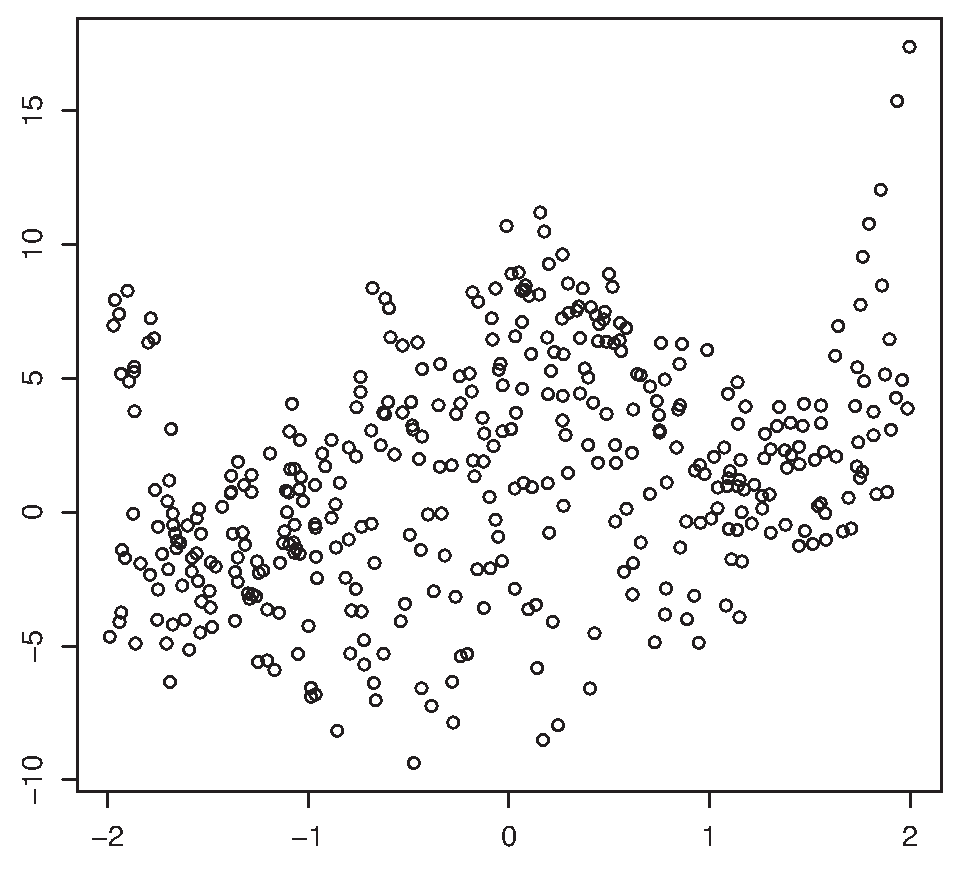
\includegraphics[width=0.8\textwidth]{img/coplot1.eps}}
  \caption{Projection of a trivariate data set onto the $xy$ plane. 
    How does the data vary with the third variable?}
  \label{fig:coplot1}
\end{figure}

Two decisions need to be made with regard to the slicing:
\begin{enumerate}
\item By what method should the overall parameter range be cut into
  slices?
\item Should slices overlap or not?
\end{enumerate}

In many ways, the most ``natural'' answer to these questions would be
to cut the entire parameter range into a set of adjacent intervals of
equal width. It is interesting to observe (by looking at the top panel
in Figure \ref{fig:coplot2}) that in the example graph, a different
decision was made in regard to both questions! The slices are 
not of equal width in the range of parameter values that they span;
instead, they have been made in such a way that each slice contains
\emph{the same number of points}. Furthermore, the slices are not
adjacent but partially overlap each other.

The first decision (to have each slice contain the same number of
points, instead of spanning the same range of values) is particularly
interesting because it provides additional\vadjust{\pagebreak} information on how the
values of the parameter $a$ are distributed. For instance, we can see
that large values of $a$ (larger than about $a=-1$) are relatively
rare, whereas values of $a$ between $-4$ and $-2$ are much more
frequent. This kind of behavior would be much harder to recognize
precisely if we had chopped the interval for $a$ into six slices of
equal width. The other decision (to make the slices overlap partially)
is more important for small data sets, where otherwise each slice
contains so few points that the structure becomes hard to see.  Having
the slices overlap makes the data ``go farther'' than if the slices
were entirely disjunct.

Co-plots are especially useful if some of the variables in a data set
are clearly ``control'' variables, because co-plots provide a
systematic way to study the dependence of the remaining (``response'')
variables on the controls.
\index{multiplots!coplots|)} 
\index{coplots|)} 


\begin{figure}
  \centerline{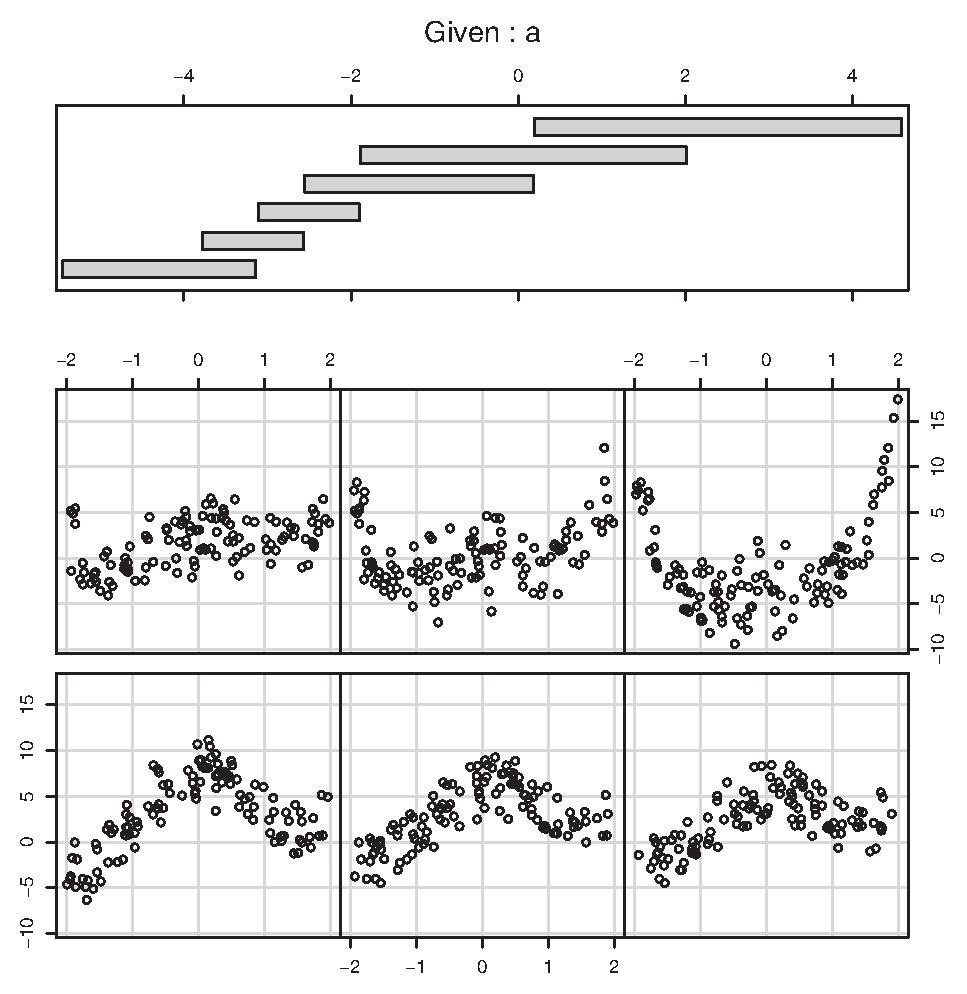
\includegraphics[width=0.8\textwidth]{img/coplot2.eps}}
  \caption{A co-plot of the same data as in Figure \ref{fig:coplot1}.
    Each scatter plot includes the data points for only a certain
    range of $a$ values; the corresponding values of $a$ are shown in
    the top panel.  (The scatter plot for the smallest value of $a$ is
    in the lower left corner, and that for the largest value of $a$ is
    in the upper right.)}
  \label{fig:coplot2}\vspace*{-6pt}
\end{figure}

\vspace*{-6pt}
\subsection{Variations}

The ideas behind scatter-plot matrices and co-plots are pretty 
generally applicable, and you can develop different variants
depending on your needs and tastes. Here are some ideas:

\begin{itemize}
\item In the standard scatter-plot matrix, half of the individual
  graphs are redundant. You can remove the individual graphs from half
  of the overall matrix and replace them with something
  different---for example, the numerical\vadjust{\pagebreak} value of the appropriate
  correlation coefficient.  However, you will then lose the ability to
  visually scan a full row or column to see how the corresponding
  quantity correlates with all other variables.
\item Similarly, you can place a histogram showing the distribution
  of values for the quantity in question on the diagonal of the 
  scatter-plot matrix.\index{histograms!scatter-plot matrices}
\item The slicing technique used in co-plots can be used with other
  graphs besides scatter plots. For instance, you might want to use
  slicing with rank-order plots (see Chapter \ref{ch:univariate}),
  where the conditioning ``parameter'' is some quantity not explicitly
  shown in the rank-order plot itself. Another option is to use it
  with histograms, making each subplot a histogram of a subset of the
  data where the subset is determined by the values of the control
  ``parameter'' variable.
\item Finally, co-plots can be extended to \emph{two} conditioning
  variables, leading to a matrix of individual slices.
\end{itemize}

By their very nature, all multiplots consist of many individual plot
elements, sometimes with nontrivial interactions (such as\vadjust{\pagebreak} the
overlapped slicing in certain co-plots). Without a good tool that
handles most of these issues automatically, these plot types lose
most of their appeal. For the plots in this section, I used R (the
statistical package), which provides support for both scatter-plot
matrices and co-plots as built-in functionality.

\index{multivariate analysis!multiplots|)} 
\index{multiplots|)} 

\vspace*{-6pt}
% ============================================================
\section{Composition Problems}

\index{multivariate analysis!composition problems|(} 
\index{composition, multivariate analysis|(} 

Many data sets describe a \emph{composition problem}; in other words,
they describe how some overall quantity is composed out of its parts.
Composition problems pose some special challenges because often we
want to visualize two \emph{different} aspects of the data
simultaneously: on the one hand, we are interested in the relative
magnitude of the different components, and on the other,  we also care
about their absolute size.

For one-dimensional problems, this is not too difficult (see Chapter
\ref{ch:univariate}). We can use a histogram or a similar graph to
display the absolute size for all components; and we can use a
cumulative distribution plot (or even the much-maligned pie chart) to
visualize the relative contribution that each component makes to the
total.

But once we add additional variables into the mix, things can get
ugly. Two problems stand out: how to visualize \emph{changes} to the
composition over time and how to depict the breakdown of an overall
quantity along \emph{multiple axes} at the same time.

\vspace*{-6pt}
\subsection{Changes in Composition}

To understand the difficulties in tracking compositional problems over
time, imagine a company that makes five products labeled A, B, C, D,
and E. As we track the daily production numbers over time, there are
two different questions that we are likely to be interested in: on the
one hand, we'd like to know how many items are produced overall; on
the other hand, we would like to understand how the item mix is
changing over time.

\begin{figure}
  \centerline{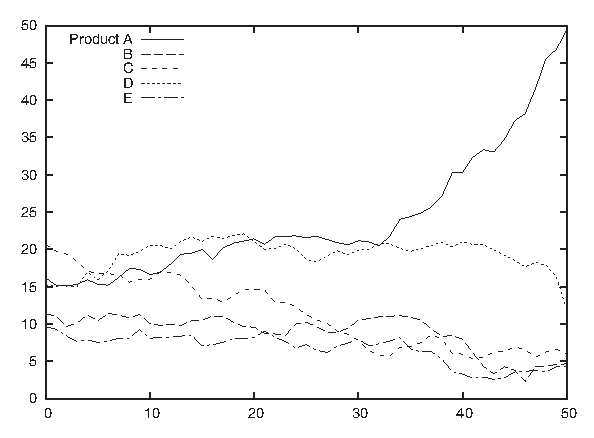
\includegraphics{img/composition1}}
  \caption{Absolute number of items produced per product line and day.}
  \label{fig:composition1}
\end{figure}

Figures \ref{fig:composition1}, \ref{fig:composition2}, and
\ref{fig:composition3} show three attempts to plot this kind of data.
Figure \ref{fig:composition1} simply shows the absolute numbers
produced per day for each of the five product lines. That's not
ideal---the graph looks messy because some of the lines obscure each
other.  Moreover, it is not possible to understand from this graph how
the total number of items changes over time. Test yourself: does the
total number of items go up over time, does it go down, or does it
stay about even?

Figure \ref{fig:composition2} is a \emph{stacked plot} \index{stacked plots} of the same
data. The daily numbers for each product are added to the numbers for
the products that appear lower down in the diagram---in other words,
the line labeled B gives the number of items produced in product lines
A \emph{and} B. The topmost line in this diagram shows the total
number of items produced per day (and answers the question posed in
the previous paragraph: the total number of items does \emph{not}
change appreciably over the long run---a possibly surprising
observation, given the appearance of Figure \ref{fig:composition1}).

\begin{figure}
  \centerline{\includegraphics{img/composition2}}
  \caption{Stacked graph of the number of items produced per product
    line and day.}
  \label{fig:composition2}
\end{figure}

Stacked plots can be compelling because they have intuitive appeal and
appear to be clear and uncluttered. In reality, however,\vadjust{\pagebreak} they tend to
hide the details in the development of the individual components
because the changing baseline makes comparison difficult if not
impossible.  For example, from Figure \ref{fig:composition1} it is
pretty clear that production of item D increased for a while but then
dropped rapidly over the last 5 to 10 days. We would never guess this
fact from Figure \ref{fig:composition2}, where the strong growth of
product line A masks the smaller changes in the other product lines.
(This is why you should order the components in a stacked graph in
ascending order of variation---which was intentionally \emph{not} done
in Figure \ref{fig:composition2}.)

Figure \ref{fig:composition3} shows still another attempt to visualize
this data. This figure is also a stacked graph, but now we are looking
not at the absolute numbers of items produced but instead at the
relative fraction that each product line contributes to the daily
total. Because the change in the total number of items produced has
been eliminated, this graph can help us understand how the item mix
varies over time (although we still have the changing baseline problem
common to all stacked graphs). However, information about the total
number of items produced has been lost.

\begin{figure}
  \centerline{\includegraphics{img/composition3}}
  \caption{Stacked graph of the relative contribution that each
    product line makes to the total.}
  \label{fig:composition3}\vspace*{-6pt}
\end{figure}

All things considered, I don't think any one of these graphs succeeds
very well. No single graph can satisfy both of our conflicting
goals---to monitor both absolute numbers as well as relative
contributions---and be clear and visually attractive at the same time.

I think an acceptable solution for this sort of problem will always
involve a combination of graphs---for example, one for the total
number of items produced and another for the relative item mix.
Furthermore, despite their aesthetic appeal, stacked graphs should be
avoided because they make it too difficult to recognize relevant
information in the graph. A plot such as Figure \ref{fig:composition1}
may seem messy, but at least it can be read accurately and reliably.

\subsection{Multidimensional Composition: Tree and Mosaic Plots}

\index{tree plots, multidimensional composition|(} 
\index{mosaic plots, multidimensional composition|(} 

Composition problems are generally difficult even when we do not worry
about changes over time. Look at the following data:

\begin{verbatim}
Male    BS      NYC     Engineering
Male    MS      SFO     Engineering
Male    PhD     NYC     Engineering
\end{verbatim}
\begin{verbatim}
Male    BS      LAX     Engineering
Male    MS      NYC     Finance
Male    PhD     SFO     Finance
Female  PhD     NYC     Engineering
Female  MS      LAX     Finance
Female  BS      NYC     Finance
Female  PhD     SFO     Finance
\end{verbatim}

The data set shows information about ten employees of some company,
and for each employee, we have four pieces of information: gender,
highest degree obtained, office where they are located (given by
airport code---NYC: New York, SFO: San Francisco, LAX: Los Angeles),
and their department. Keep in mind that each line corresponds to a
single person.

The usual way to summarize such data is in the form of a \emph{contingency
  table}. \index{contingency tables} Table \ref{tbl:mosaicplot} summarizes what we know about the
relationship between an employee's gender and his or her department.
Contingency tables are used to determine whether there is a correlation
between categorical variables: in this case, we notice that men tend
to work in engineering and women in finance. (We may want to divide
by the total number of records to get the \emph{fraction} of employees
in each cell of the table.)

\begin{table}[b]
\def\a{\hphantom{0}}
\def\vrl{\smash{\vrule height48.6pt  width.25pt depth5pt}}
\tbl{A contingency table: breakdown of male and female employees
  across two departments\label{tbl:mosaicplot}}{%
\begin{tabular}{l@{\hskip9pt}c@{\hskip9pt}cc@{\hskip9pt}c@{\hskip9pt}c}\toprule
                               && \TCH{Male} & \TCH{Female} && \TCH{Total} \\\colrule
Engineering     && 4    & 1      && \a5  \\
Finance         && 2    & 3      && \a5 \\\colrule
\textbf{Total}  &\vrl& 6    & 4      &\vrl& 10\\\botrule
\end{tabular}}
\end{table}

The problem is that contingency tables only work for two dimensions at
a time. If we also want to include the breakdown by degree or
location, we have no other choice than to repeat the basic structure
from Table \ref{tbl:mosaicplot} several times: once for each office or
once for each degree.

A \emph{mosaic plot} is an attempt to find a graphical representation
for this kind of data. The construction of a mosaic plot is
essentially recursive and proceeds as follows (see Figure
\ref{fig:mosaicplots}):

\begin{enumerate}
\item Start with a square.
\item Select a dimension, and then divide the square proportionally
  according to the counts for this dimension.
\item Pick a second dimension, and then divide each subarea according
  to the counts along the second dimension, separately for each
  subarea.
\item Repeat for all dimensions, interchanging horizontal and vertical
  subdivisions for each new dimension.
\end{enumerate}

In the lower left panel of Figure \ref{fig:mosaicplots}, location is shown as a secondary vertical subdivision in 
addition to the gender (from left to right: LAX, NYC, SFO). In
addition, the degree is shown through shading (shaded sections
correspond to employees with a Ph.D.).

\begin{figure}
  \begin{tabular}{@{\hskip-12pt}cc}
    \includegraphics[width=2.5in]{img/mosaic1} &
    \includegraphics[width=2.5in]{img/mosaic2} \\[6pt]
    \includegraphics[width=2.5in]{img/mosaic3} &
    \includegraphics[width=2.5in]{img/mosaic4} 
  \end{tabular}
  \caption{Mosaic plots. In the top row, we start by dividing by 
    gender, then also by department. In the bottom row, we have
    divided by gender, department, and location, with doctorate
    degrees shaded. The graph on the left uses the same sort order
    of dimensions as the graphs in the top row, whereas the graph
    on the bottom right uses a different sort order. Notice how
    the sort order changes the appearance of the graph!}
  \label{fig:mosaicplots}
\end{figure}

Having seen this, we should ask how much mosaic plots actually help us
understand this data set.  Obviously, Figure \ref{fig:mosaicplots} is
difficult to read and has to be studied carefully. Keep in mind that
the information about the number of data points within each category
is represented by the area---recursively at all levels. Also note that
some categories are empty and therefore invisible (for instance, there
are no female employees in either the Los Angeles or San Francisco
engineering departments).

I appreciate mosaic plots because they represent a new idea for how
data can be displayed graphically, but I have not found them to be
useful.  In my own experience, it is easier to understand a data set
by poring over a set of contingency tables than by drawing mosaic
plots.  Several problems stand out.

\begin{itemize}
\item The order in which the dimensions are applied matters greatly
  for the appearance of the plot. The lower right panel in Figure
  \ref{fig:mosaicplots} shows the same data set yet again, but this
  time the data was split along the location dimension first and
  along the gender dimension last.  Shading again indicates employees
  with a Ph.D. Is it obvious that this is the same data set? Is one
  representation more helpful than the other?
\item Changing the sort order changes more than just the appearance, it
  also influences what we are likely to recognize in the graph. Yet
  even with an interactive tool, I find it thoroughly confusing to
  view a large number of mosaic plots with changing layouts. 
\item It seems that once we have more than about four or five
  dimensions, mosaic plots become too cluttered to be useful. This is
  not a huge advance over the two dimensions presented in basic
  contingency tables!
\item Finally, there is a problem common to all visualization methods
  that rely on \emph{area} to indicate magnitude: human perception is
  not that good at comparing areas, especially areas of different
  shape. In the lower right panel in Figure \ref{fig:mosaicplots}, for
  example, it is not obvious that the sizes of the two shaded areas
  for engineering in NYC are the same. (Human perception works by
  comparing visual objects to each other, and the easiest to compare
  are lengths, not areas or angles. This is also why you should favor
  histograms over pie charts!)
\end{itemize}

In passing, let's quickly consider a different but related concept:
\emph{tree maps}. Tree maps are area-based representations of
hierarchical tree structures.  As shown in Figure \ref{fig:treemaps},
the area of each parent node in the tree is divided according to the
weight of its children.

\begin{figure}
  \begin{tabular}{ccc}
    \includegraphics[width=2in]{img/treemap1} &
    \hspace{1cm}
    \includegraphics{img/treemap2} 
  \end{tabular}
  \caption{A tree map (left) and the corresponding tree (right). The
    numbers give the weight of each node and, if applicable, also the
    weight of the entire subtree.}
  \label{fig:treemaps}
\end{figure}\pagebreak

Tree maps are something of a media phenomenon.  Originally developed
for the purpose of finding large files in a directory hierarchy, they
seem to be more talked about then used. They share the problems of all
area-based visualizations already discussed, and even their inventors
report that people find them hard to read---especially if the number
of levels in the hierarchy increases. Tree maps lend themselves well
to interactive explorations (where you can ``zoom in'' to deeper
levels of the hierarchy).

My greatest concern is that tree maps have abandoned the primary
advantage of graphical methods without gaining sufficiently in power,
namely \emph{intuition}: looking at a tree map does not conjure up the
image of, well, a \emph{tree}! (I also think that the focus on
treelike hierarchies is driven more by the interests of computer
science, rather than by the needs of data analysis---no wonder if the
archetypical application consisted of browsing a file system!)

\index{tree plots, multidimensional composition|)} 
\index{mosaic plots, multidimensional composition|)} 
\index{multivariate analysis!composition problems|)} 
\index{composition, multivariate analysis|)} 

% ============================================================
\section{Novel Plot Types}

Most of the graph types I have described so far (with the exception of
mosaic plots) can be described as ``classical'': they have been around
for years. In this section, we will discuss a few techniques that are
much more recent---or, at least, that have only recently received
greater attention.

\subsection{Glyphs}

\index{multivariate analysis!glyphs|(} 
\index{glyphs}
 
We can include additional information in any simple plot (such as a
scatter plot) if we replace the simple symbols used for individual
data points with \emph{glyphs}: more complicated symbols that can
express additional bits of information by themselves.

An almost trivial application of this idea occurs if we put two data
sets on a single scatter plot and use different symbols (such as
squares and crosses) to mark the data points from each data set.  Here
the symbols themselves carry meaning but only a simple, categorical
one---namely, whether the point belongs to the first or second data
set.

But if we make the symbols more complicated, then they can express
more information.  Textual labels (letters and digits) are often
surprisingly effective when it comes to conveying more
information---although distinctly low-tech, this is a technique to
keep in mind!

The next step up in sophistication are arrows, which can represent
both a direction and a magnitude (see Figure \ref{fig:vectorplot}), but
we need not stop there. Each symbol can be a fully formed graph (such
as a pie chart or a histogram) all by itself. And even that is not the
end---probably the craziest idea in this realm are ``Chernoff faces,''
where different quantities are encoded as \emph{facial features} (\eg,
size of the mouth, distance between the eyes), and the faces are used
as symbols on a plot!

As you can see, the problem lies not so much in putting more
information on a graph as in being able to interpret the result in a
useful manner. And that seems to depend mostly on the \emph{data}, in
particular on the presence of large-scale, regular structure in it.
If such structure is missing, then plots using glyphs can be very hard
to decode and quite possibly useless.

\begin{figure}
  \centerline{\includegraphics{img/vectorplot}}
  \caption{Simple glyphs: using arrows to indicate both direction and
    magnitude of a field. Notice that the variation in the data is
    smooth and that the data itself has been recorded on a regular
    grid.}
  \label{fig:vectorplot}\vspace*{-6pt}
\end{figure}

Figures \ref{fig:vectorplot} and \ref{fig:glyphplot} show two extreme
examples. In Figure \ref{fig:vectorplot}, we visualize a
four-dimensional data set using arrows (each point of the
two-dimensional plot area has both a direction and a magnitude, so the
total number of dimensions is four). You can think of the system as
flow in a liquid, as electrical or magnetic field lines, or as
deformations in an elastic medium---it does not matter, the overall
nature of the data becomes quite clear. But Figure \ref{fig:glyphplot}
is an entirely different matter! Here we are dealing with a data set
in seven dimensions: the first two are given by the position of the
symbol on the plot, and the remaining five are represented via
distortions of a five-edged polygon.  Although we can make out some
regularities (\eg, the shapes of the symbols in the lower lefthand
corner are all quite similar and different from the shapes elsewhere),
this graph is hard to read and does not reveal the overall
structure of the data very well. Also keep in mind that the
appearance of the graph will change if we map a different pair of
variables to the main axes of the plot, or even if we change the order
of variables in the polygons.

\begin{figure}
   \centerline{\includegraphics{img/glyphplot}}
  \caption{Complex glyphs: each polygon encodes five different
    variables, and its position on the plot adds another two.}
  \label{fig:glyphplot}
\end{figure}

\vspace*{-6pt}
\subsection{Parallel Coordinate Plots}

\index{multivariate analysis!parallel coordinate plots|(}
\index{parallel coordinate plots|(}  

As we have seen, a scatter plot can show two variables. If we use
glyphs, we can show more, but not\vadjust{\pagebreak} all variables are treated equally
(some are encoded in the glyphs, some are encoded by the position of
the symbol on the plot). By using \emph{parallel coordinate plots}, we
can show all the variables of a multivariate data set on equal footing.
The price we pay is that we end up with a graph that is neither pretty
nor particularly intuitive, but that can be useful for exploratory
work nonetheless.

In a regular scatter plot in two (or even three) dimensions, the
coordinate axes are at right angles to each other. In a parallel
coordinate plot, the coordinate axes instead are \emph{parallel} to
each other. For every data point, its value for each of the variables
is marked on the corresponding axis, and then all these points are
connected with lines. Because the axes are parallel to each other, we
don't run out of spatial dimensions and therefore can have as many
of them as we need. Figure \ref{fig:parallel1} shows what a single
record looks like in such a plot, and Figure \ref{fig:parallel2} shows
the entire data set. Each record consists of nine different quantities
(labeled A through J).

\begin{figure}
   \centerline{\includegraphics{img/parallel1}}
  \caption{A single record (\ie, a single data point) from a
    multivariate data set shown in a parallel coordinate plot.}
  \label{fig:parallel1}\vspace*{-6pt}
\end{figure}

The main use of parallel coordinate plots is to find clusters in
high-dimensional data sets. For example, in Figure \ref{fig:parallel2},
we can see that the data forms two clusters for the quantity labeled
B: one around $0.8$ and one around $0$. Furthermore, we can see that 
most records for which B is $0$, tend to have higher values of C 
than those that have a B near $0.8$. And so~on.

\begin{figure}
   \centerline{\includegraphics{img/parallel2}}
  \caption{All records from the data set shown in a parallel
    coordinate plot. The record shown in Figure \ref{fig:parallel1} is
    highlighted.}
  \label{fig:parallel2}\vspace*{-6pt}
\end{figure}

A few technical points should be noted about parallel coordinate
plots:

\begin{itemize}
\item You will usually want to rescale the values in each
  coordinate to the unit interval via the linear transformation
  (also see Appendix \ref{app:calculus}):
  % 
  \[
  x_{{\rm scaled}} 
    = \frac{x - x_{{\rm min}}}{x_{{\rm max}} - x_{{\rm min}}}
  \]
  % 
  This is not mandatory, however. There may be situations where
  you care about the absolute positions of the points along the
  coordinate axis or about scaling to a different interval.
\item The appearance of parallel coordinate plots depends strongly on
  the order in which the coordinate lines are drawn: rearranging them
  can hide or reveal structure. Ideally, you have access to a tool
  that lets you reshuffle the coordinate axis interactively.
\item Especially for larger data sets (several hundreds of points
  or more), overplotting of lines becomes a problem. One way to deal
  with this is through ``alpha blending'': lines are shown as
  semi-transparent, and their visual effects are combined where they
  overlap each other.
\item Similarly, it is often highly desirable to be able to select a
  set of lines and highlight them throughout the entire graph---for
  example, to see how data points that are clustered in one dimension
  are distributed in the other dimensions.
\item Instead of combining points on adjacent coordinate axes with
  straight lines that have sharp kinks at the coordinate axes, one
  can use smooth lines that pass the coordinate axes without kinks.
\end{itemize}

All of these issues really are \emph{tool} issues, and in fact
parallel coordinates don't make sense without a tool that supports
them natively and includes good implementations of the features just
described. This implies that parallel coordinate plots serve less as
finished, static graphs than as an interactive tool for exploring a
data set.

Parallel coordinate plots still seem pretty novel. The idea itself has
been around for about 25 years, but even today, tools that support
parallel coordinates plots \emph{well} are far from common place.

What is not yet clear is how useful parallel coordinate plots really
are. On the one hand, the concept seems straightforward and easy
enough to use. On the other hand, I have found the experience of
actually trying to apply them frustrating and not very fruitful. It is
easy to get bogged down in technicalities of the plot (ordering and
scaling of coordinate axes) with little real, concrete insight
resulting in the end. The erratic tool situation of course does not
help.  I wonder whether more computationally intensive methods (\eg,
principal component analysis---see Chapter \ref{ch:reduction}) do not
give a better return on investment overall.  But the jury is still
out.
\index{multivariate analysis!parallel coordinate plots|)}%
\index{parallel coordinate plots|)}%

\vspace*{-6pt}
% ============================================================
\section{Interactive Explorations}

\index{multivariate analysis!interactive explorations|(} 

All the graphs that we have discussed so far (in this and the
preceding chapters) were by nature \emph{static}. We prepared graphs,
so that we then could study them, but this was the extent of our
interaction.  If we wanted to see something different, we had to
prepare a new graph.

In this section, I shall describe some ideas for \emph{interactive}
graphics: graphs that we can change directly in some way without
having to re-create them anew.

Interactive graphics cannot be produced with paper and pencil, not
even in principle: they \emph{require} a computer. Conversely, what we
can do in this area is even more strongly limited by the tools or
programs that are available to us than for other types of graphs. In
this sense, then, this section is more about \emph{possibilities} than
about \emph{realities} because the tool support for interactive
graphical exploration seems (at the time of this writing) rather poor.

\subsection{Querying and Zooming}

\index{querying and zooming, multivariate analysis}
\index{zooming and querying, multivariate analysis} 

Interaction with a graph does not have to be complicated. A very
simple form of interaction consists of the ability to select a point
(or possibly a group of points) and have the tool display additional
information about it. In the simplest case, we hover the mouse pointer
over a data point and see the coordinates (and possibly additional
details) in a tool tip or a separate window. We can refer to this
activity as \emph{querying}.

Another simple form of interaction would allow us to change aspects of
the graph directly using the mouse.  Changing the plot range (\ie,
\emph{zooming}) is probably the most common application, but I could
also imagine to adjust the aspect ratio, the color palette, or
smoothing parameters in this way. (Selecting and highlighting a subset
of points in a parallel coordinate plot, as described earlier, would
be another application.)

Observe that neither of these activities is inherently
``interactive'': they all would also be possible if we used paper and
pencil. The interactive aspect consists of our ability to invoke them
in real time and by using a graphical input device (the mouse).

\vspace*{-9pt}
\subsection{Linking and Brushing}

\index{linking and brushing, multivariate analysis}
\index{brushing and linking, multivariate analysis}
  
The ability to interact directly with graphs becomes much more
interesting once we are dealing with multiple graphs at the same time!
For example, consider a scatter-plot matrix like the one in Figure
\ref{fig:splom}. Now imagine we use the mouse to select and highlight
a group of points in one of the subplots. If the graphs are
\emph{linked}, then the symbols corresponding to the data points
selected in one of the subplots will also be highlighted in all other
subplots as well.

% --- XXX : need a ref to an example here

Usually selecting some points and then highlighting their
corresponding symbols in the linked subgraphs requires two separate
steps (or mouseclicks). A real-time version of the same idea is called
\emph{brushing}: any points currently under the mouse pointer are
selected and highlighted in all of the linked subplots.

Of course, linking and brushing are not limited to scatter-plot
matrices, but they are applicable to any group of graphs that show
different aspects of the same data set.  Suppose we are working with a
set of histograms of a multivariate data set, each histogram showing
only one of the quantities.  Now I could imagine a tool that allows us
to select a bin in \emph{one} of the histograms and then highlights
the contribution from the points in that bin in all the other
histograms.

% --- XXX : need a ref to an example here
\vspace*{-9pt}
\subsection{Grand Tours and Projection Pursuits}

\index{grand tours and projection pursuits, multivariate analysis}
\index{projection pursuits and grand tours, multivariate analysis}
 
Although linking and brushing allow us to interact with the data, they
leave the graph itself static. This changes when we come to
\emph{Grand Tours} and \emph{Projection Pursuits}. Now we are talking
about truly animated graphics!

Grand Tours and Projection Pursuits are attempts to enhance our
understanding of a data set by presenting many closely related\vadjust{\pagebreak}
projections in the form of an animated ``movie.'' The concept is
straightforward: we begin with some projection and then continuously
move the viewpoint around the data set. (For a three-dimensional data
set, you can imagine the viewpoint moving on a sphere that encloses
the data.)

In Grand Tours, the viewpoint is allowed to perform essentially a
random walk around the data set. In Projection Pursuits, the viewpoint
is moved so that it will improve the value of an index that measures
how ``interesting'' a specific projection will appear.  Most indices
currently suggested measure properties such as deviation from Gaussian
behavior. At each step of a Pursuit, the program evaluates several
possible projections and then selects the one that most improves the
chosen index. Eventually, a Pursuit will reach a local maximum for the
index, at which time it needs to be restarted from a different
starting point.

Obviously, Tours and Pursuits require specialized tools that can
perform the required projections---and do so in real time.  They are
also exclusively exploratory techniques and not suitable for
preserving results or presenting them to a general audience.

Although the approach is interesting, I have not found Tours to be
especially useful in practice. It can be confusing to watch a movie of
essentially random patterns and frustrating to interact with
projections when attempting to explore the neighborhood of an
interesting viewpoint.

\vspace*{-9pt}
\subsection{Tools}

\index{multivariate analysis!tools|(}
 
All interactive visualization techniques require suitable tools and
computer programs; they cannot be done using paper-and-pencil methods.
This places considerable weight on the quality of the available tools.
Two issues stand out.

\begin{itemize}
\item It seems difficult to develop tools that support interactive
  features and are sufficiently general at the same time. For example,
  if we expect the plotting program to show additional detail on any
  data point that we select with the mouse, then the input (data) file
  will have to contain this information---possibly as metadata.  But
  now we are talking about relatively complicated data sets, which
  require more complicated, structured file formats that will be
  specific to each tool. So before we can do anything with the data,
  we will have to transform it into the required format. This is a
  significant burden, and it may make these methods infeasible in
  practice.  (Several of the more experimental programs mentioned in
  the Workshop section in this chapter are nearly unusable on actual
  data sets for exactly this reason.)
\item A second problem concerns performance. Brushing, for instance,
  makes sense only if it truly occurs in real time---without any
  discernible delay as the mouse pointer moves. For a large data set
  and a scatter-plot matrix of a dozen attributes, this means updating
  a few thousand points in real time. Although by no means infeasible,
  such responsiveness does require that the tool is written with an
  eye toward performance and using appropriate technologies. (Several
  of the tools mentioned in the Workshop exhibit serious performance
  issues on real-world data sets.)
\end{itemize}

A final concern involves the overall design of the user interface. It
should be easy to learn and easy to use, and it should support the
activities that are actually required. Of course, this concern is not
specific to data visualization tools but common to all programs with
a graphical user interface.
\index{multivariate analysis!interactive explorations|)} 

\vspace*{-9pt}
% ============================================================
\section{Workshop:  Tools for Multivariate Graphics}

Multivariate graphs tend to be complicated and therefore require good
tool support even more strongly than do other forms of graphs.  In
addition, some multivariate graphics are highly specialized (\eg,
mosaic plots) and cannot be easily prepared with a general-\break purpose
plotting tool.

That being said, the tool situation is questionable at best.  Here
are three different starting points for exploration---each with its
own set of difficulties.

\vspace*{-9pt}
\subsection{R}

\index{R statistical analysis package} 
\index{software!R statistical analysis package}

R is not a plotting tool per se; it is a statistical analysis package
and a full development environment as well. However, R has always
included pretty extensive graphing capabilities. R is particularly
strong at ``scientific'' graphs: straightforward but highly accurate
line diagrams.

Because R is not simply a plotting tool, but instead a full data
manipulation and programming environment, its learning curve is rather
steep; you need to know a lot of different things before you can do
anything. But once you are up and running, the large number of
advanced functions that are already built in can make working with R
very productive. For example, the scatter-plot matrix in Figure
\ref{fig:splom} was generated using just these three commands:

\begin{verbatim}
d <- read.delim( "wines", header=T )

pairs(d)

dev.copy2eps( file="splom.eps" )
\end{verbatim}

(the R command \texttt{pairs()} generates a plot of all pairs---\ie, a
scatter-plot matrix). The scatter plot in Figure \ref{fig:coplot1} and
the co-plot in Figure \ref{fig:coplot2} were generated using:

\begin{verbatim}
d <- read.delim( "data", header=F )
names( d ) <- c( "x", "a", "y" )

plot( y ~ x, data=d )
dev.copy2eps( file='coplot1.eps' )

coplot( y ~ x | a, data=d )
dev.copy2eps( file='coplot2.eps' )
\end{verbatim}

Note that these are the \emph{entire} command sequences, which include
reading the data from file and writing the graph back to disk! We'll
have more to say about R in the Workshop sections of Chapters
\ref{ch:statistics} and \ref{ch:reduction}.

R has a strong culture of user-contributed add-on packages. For
multiplots consisting of subplots arranged on a regular grid (in
particular, for generalized co-plots), you should consider the
\texttt{lattice} package, which extends or even replaces the
functionality of the basic R graphic systems. This package is part of
the standard R distribution.

\vspace*{-6pt}
\subsection{Experimental Tools}

If you want to explore some of the more novel graphing ideas, such as
parallel coordinate plots and mosaic plots, or if you want to try out
interactive ideas such as brushing and Grand Tours, then there are
several options open to you. All of them are academic research
projects, and all are highly experimental. (In a way, this is a
reflection of the state of the field: I don't think any of these novel
plot types have been refined to a point where they are clearly
useful.)

\begin{itemize}
\item The ggobi project (\url{http://www.ggobi.org}) allows brushing
  in scatter-plot matrices and parallel coordinate plots and includes
  support for animated tours and pursuits.

\item Mondrian (\url{http://www.rosuda.org/mondrian}) is a Java
  application that can produce mosaic plots (as well as some other
  multivariate graphs).
\end{itemize}

Again, both tools are academic research projects---and it shows. They
are technology demonstrators intended to try out and experiment with
new graph ideas, but neither is anywhere near production strength.
Both are rather fussy about the required data input format, their
graphical user interfaces are clumsy, and neither includes a proper way to
export graphs to file (if you want to save a plot, you have to take a
screenshot). The interactive brushing features in ggobi are slow,
which makes them nearly unusable for realistically sized data sets.
There are some lessons here (besides the intended ones) to be learned
about the design of tools for statistical graphics. (For instance, GUI
widget sets do not seem suitable for interactive visualizations: they
are too slow. You have to use a lower-level graphics library instead.)

Other open source tools you may want to check out are Tulip
(\url{http://tulip.labri.fr}) and ManyEyes
(\url{http://manyeyes.alphaworks.ibm.com/manyeyes}). The latter
project is a web-based tool and community that allows you to upload
your data set and generate plots of it online.

A throwback to a different era is OpenDX
(\url{http://www.research.ibm.com/dx}).  Originally designed by IBM in
1991, it was donated to the open source community in 1999. It
certainly feels overly complicated and dated, but it does include a
selection of features not found elsewhere.

\vspace*{-6pt}
\subsection{Python Chaco Library}

\index{Python Chaco library!} 
\index{software!Python}
 
The Chaco library (\url{http://code.enthought.com/projects/chaco/}) is
a Python library for two-dimensional plotting. In addition\vadjust{\pagebreak} to the
usual line and symbol drawing capabilities, it includes easy support
for color and color manipulation as well as---more importantly---for
real-time user interaction.

Chaco is an exciting toolbox if you plan to experiment with writing
your own programs to visualize data and interact with it. However, be
prepared to do some research: the best available documentation seems
to be the set of demos that ship with it.

Chaco is part of the Enthought Tool Suite, which is developed by
Enthought, Inc., and is available under a BSD-style license.

\index{multivariate analysis!tools|)}

% ============================================================
\section{Further Reading}

\begin{itemize}

\item \cit{Graphics of Large Datasets: Visualizing a Million}{Antony
    Unwin, Martin Theus, and Heike Hofmann}{Springer}{2006} 
  This is a modern book that in many ways describes the state of the
  art in statistical data visualization. Mosaic plots, glyph plots,
  parallel coordinate plots, Grand Tours---all are discussed here.
  Unfortunately, the basics are neglected: standard tools like
  logarithmic plots are never even mentioned, and simple things like
  labels are frequently messed up.  This book is nevertheless
  interesting as a survey of some of the state of the art.

\item \cit{The Elements of Graphing Data}{William S.\ Cleveland}{2nd ed.,
    Hobart Press}{1994} 
  This book provides an interesting counterpoint to the book by Unwin
  and colleagues. Cleveland's graphs often look pedestrian, but he
  thinks more deeply than almost anyone else about ways to incorporate
  more (and more quantitative) information in a graph. What stands out
  in his works is that he explicitly takes human perception into
  account as a guiding principle when developing new graphs. My
  discussion of scatter-plot matrices and co-plots is heavily
  influenced by his careful treatment.

\item \cit{Gnuplot in Action: Understanding Data with Graphs}{Philipp 
    K.\ Janert}{Manning Publications}{2010}
  Chapter 9 of this book contains additional details on and examples
  for the use of color to prepare false-color plots, including
  explicit recipes to create them using gnuplot. But the principles
  are valid more generally, even if you use different tools.

\item 
{\it Why Should Engineers and Scientists Be Worried About
    Color?} {B.\ E.\ Rogowitz and L.\ A.\
    Treinish.} {\url{http://www.research.ibm.com/people/l/lloydt/color/color.HTM}.} {1995.}
  This paper contains important lessons for false-color plots,
  including the distinction between segmentation and smooth variation
  as well as the difference between hue- and luminance-based palettes.
  The examples were prepared using IBM's (now open source) OpenDX
  graphical Data Explorer.

\item \cit{Escaping RGBland: Selecting Colors for Statistical
    Graphics}{A.\ Zeileis, K.\ Hornik, and 
P.~Murrell}{\url{http://statmath.wu.ac.at/}$\sim$\url{zeileis/papers/Zeileis+Hornik+Murrell-2009.pdf}}{2009}
  This is a more recent paper on the use of color in graphics. It
  emphasizes the importance of perception-based color spaces, such as
  the HCL model.
\end{itemize}

\index{data analysis!multivariate analysis|)} 
\index{multivariate analysis|)} 

\clearpage

\thispagestyle{empty}

\cleardoublepage % done

% Mikes: ok
% Spellcheck: ok

% ============================================================
\chapter{Intermezzo: A Data Analysis Session}{}{}
\label{ch:session}
  
\index{data analysis!session example|(}
   
\Fint{Occasionally I get the question: ``How do you actually work?''  or
``How do you come up with this} stuff?'' As an answer, I want to take
you on a tour through a new data set. I will use gnuplot, \index{plot function (gnuplot)} which is my
preferred tool for this kind of interactive data analysis---you will
see why. And I will share my observations and thoughts as we go along.

\section{A Data Analysis Session}
    
The data set is a classic: the $\mathrm{CO_2}$ measurements above
Mauna Loa on Hawaii. \index{CO2@$\mathrm{CO_2}$ measurements above Mauna Loa on Hawaii} The inspiration for this section comes from
Cleveland's \emph{Elements of Graphical Analysis},\footnote{\cit{The
    Elements of Graphing Data}{William S.\ Cleveland}{Hobart
    Press}{1994. The data itself (in a slightly different format) is
  available from StatLib:
  \url{http://lib.stat.cmu.edu/datasets/visualizing.data.zip} and from
  many other places around the Web}} but the approach is entirely
mine.
    
First question: what's in the data set? I see that the first column
represents the date (month and year) while the second contains the
measured $\mathrm{CO_2}$ concentration in parts per million. Here are
the first few lines:

\begin{verbatim}
Jan-1959        315.42
Feb-1959        316.32
Mar-1959        316.49
Apr-1959        317.56
...
\end{verbatim}

The measurements are regularly spaced (in fact, monthly), so I don't
need to parse the date in the first column; I simply\vadjust{\pagebreak} plot the second
column by itself. (In the figure, I have added tick labels on the
horizontal axis for clarity, but I am omitting the commands required
here---they are not essential.)

\begin{verbatim}
plot "data" u 1 w l
\end{verbatim}

The plot shows a rather regular short-term variation overlaid on a
nonlinear upward trend. (See Figure \ref{fig:session01}.)

\begin{figure}[t!]
  \centerline{\includegraphics{img/session01}}
  \caption{The first look at the data: \hbox{\em plot ``data'' u 1 w l}}
  \label{fig:session01}
\end{figure}
    
The coordinate system is not convenient for mathematical modeling: the
$x$ axis is not numeric, and for modeling purposes it is usually helpful
if the graph goes through the origin. So, let's make it do so by
subtracting the vertical offset from the data and expressing the
horizontal position as the number of months since the first
measurement.  (This corresponds to the line number in the data file,
which is accessible in a gnuplot session through the pseudo-column
with column number 0.) 

\begin{verbatim}
plot "data" u 0:($2-315) w l
\end{verbatim}

A brief note on the command: the specification after the \texttt{u}
(short for \texttt{using}) gives the columns to be used for the $x$
and $y$ coordinates, separated by a colon. Here we use the line number
(which is in the pseudo-column 0) for the $x$ coordinate.  Also, we
subtract the constant offset 315 from the values in the second column
and use the result as the $y$ value. Finally, we plot the result
\texttt{with lines} (abbreviated \texttt{w l}) instead of using points
or other symbols. See Figure \ref{fig:session02}.

\begin{figure}[t!]
  \centerline{\includegraphics{img/session02}}
  \caption{Making the $x$ values numeric and subtracting the constant
    vertical offset: \hbox{\em plot ``data'' u 0:(\$2-315) w l}}
  \label{fig:session02}
\end{figure}
    
The most predominant feature is the trend. \index{trends!$\mathrm{CO_2}$ measurements above Mauna Loa on Hawaii} What can we say about it?
First of all, the trend is nonlinear: if we ignore the short-term
variation, the curve is convex downward. This suggests a power law
with an as-yet-unknown exponent: $x^k$. All power-law functions go
through the origin $(0,0)$ and also through the point $(1,1)$. We
already made sure that the data passes through the origin, but to fix
the upper-right corner, we need to rescale both axes: if $x^k$ goes
through $(1,1)$, then $b \paren{ \frac{x}{a} }^k$ goes through
$(a,b)$.
    
What's the value for the exponent $k$? All I know about it right now
is that it must be greater than 1 (because the function is convex).
Let's try $k=2$. (See Figure \ref{fig:session03}.)

\begin{verbatim}
plot "data" u 0:($2-315) w l, 35*(x/350)**2
\end{verbatim}

\begin{figure}[t!]
  \centerline{\includegraphics{img/session03}}
  \caption{Adding a function: \hbox{\em plot ``data'' u 0:(\$2-315) w l,
      35*(x/350)**2}}
  \label{fig:session03}
\end{figure}
    
Not bad at all! The exponent is a bit too large---some fiddling
suggests that $k=1.35$ would be a good value (see Figure
\ref{fig:session04}).

\begin{verbatim}
plot "data" u 0:($2-315) w l, 35*(x/350)**1.35
\end{verbatim}

\begin{figure}[t!]
  \centerline{\includegraphics{img/session04}}
  \caption{Getting the exponent right: 
    $f(x) = 35 \paren{\frac{x}{350}}^{1.35}$}
  \label{fig:session04}
\end{figure}
    
To verify this, let's plot the residual; that is, we subtract the
trend from the data and plot what's left. If our guess for the trend
is correct, then the residual should not exhibit any trend itself---it
should just straddle $y=0$ in a balanced fashion (see Figure
\ref{fig:session05}).

\begin{verbatim}
plot "data" u 0:($2-315 - 35*($0/350)**1.35) w l
\end{verbatim}

\begin{figure}[t!]
  \centerline{\includegraphics{img/session05}}
  \caption{The residual, after subtracting the function from the data.}
  \label{fig:session05}
\end{figure}
    
It might be hard to see the longer-term trend in this data, so we may
want to approximate it by a smoother curve. We can use the
weighted-spline approximation built into gnuplot for that purpose.  It
takes a third parameter, which is a measure for the smoothness: the
smaller the third parameter, the smoother the resulting curve; the
larger the third parameter, the more closely the spline follows the
original data (see Figure~\ref{fig:session06}).

\makeatletter
\def\texttt#1{{\fontsize{8}{10}\ttfamily\selectfont#1}}
\makeatother

\hspace*{18pt}\texttt{plot "data" u 0:($2-315 - 35*($0/350)**1.35) w l,
$\backslash$}\vspace*{-4pt}
\begin{verbatim}
     "" u 0:($2-315 - 35*($0/350)**1.35):(0.001) s acs w l
\end{verbatim}

\makeatletter
\def\texttt#1{{\fontsize{8.5}{10}\ttfamily\selectfont#1}}
\makeatother
    
At this point, the expression for the function that we use to
approximate the data has become unwieldy. Thus it now makes sense to
define it as a separate function:

\begin{verbatim}
f(x) = 315 + 35*(x/350)**1.35
plot "data" u 0:($2-f($0)) w l, "" u 0:($2-f($0)):(0.001) s acs w l
\end{verbatim}

\begin{figure}[t!]
  \centerline{\includegraphics{img/session06}}
  \caption{Plotting a smoothed version of the residual together with
    the unsmoothed residual to test whether there is any systematic
    trend remaining in the residual.}
  \label{fig:session06}
\end{figure}

From the smoothed line we can see that the overall residual is pretty
much flat and straddles zero. Apparently, we have captured the overall
trend quite well: there is little evidence of a systematic drift
remaining in the residuals.

With the trend taken care of, the next feature to tackle is the
seasonality. \index{seasonality!$\mathrm{CO_2}$ measurements above Mauna Loa on Hawaii} The seasonality seems to consist of rather regular
oscillations, so we should try some combination of sines and cosines.
The data pretty much starts out at $y=0$ for $x=0$, so we can try a
sine by itself. To make a guess for its wavelength, we recall that the
data is meteorological and has been taken on a monthly basis---perhaps
there is a year-over-year periodicity. This would imply that the data
is the same every $12$ data points. If so, then a full period of the
sine, which corresponds to $2\pi$, should equal a horizontal distance
of $12$ points. For the amplitude, the graph suggests a value close to
$3$ (see Figure \ref{fig:session07}).

\begin{verbatim}
plot "data" u 0:($2-f($0)) w l, 3*sin(2*pi*x/12) w l
\end{verbatim}

\begin{figure}[t!]
  \centerline{\includegraphics{img/session07}}
  \caption{Fitting the seasonality with a sine wave: 
    $3 \sin\paren{2\pi \frac{x}{12}}$}
  \label{fig:session07}\vspace*{-6pt}
\end{figure}
  
Right on! In particular, our guess for the wavelength worked out
really well. This makes sense, given the origin of the data.
    
Let's take residuals again, employing splines to see the bigger
picture as well (see Figure \ref{fig:session08}):

\begin{verbatim}
f(x) = 315 + 35*(x/350)**1.35 + 3*sin(2*pi*x/12)
plot "data" u 0:($2-f($0)) w l, "" u 0:($2-f($0)):(0.001) s acs w l
\end{verbatim}

\begin{figure}[t!]
  \centerline{\includegraphics{img/session08}}
  \caption{Residuals after subtracting both trend and seasonality.}
  \label{fig:session08}\vspace*{-6pt}
\end{figure}
    
The result is pretty good but not good enough. There is clearly some
regularity remaining in the data, although at a higher frequency than
the main seasonality. Let's zoom in on a smaller interval of the data
to take a closer look. The data in the interval \texttt{[60:120]}
appears particularly regular, so let's look there (see Figure
\ref{fig:session09}):

\begin{verbatim}
plot [60:120] "data" u 0:($2-f($0)) w lp, "" u 0:($2-f($0)):(0.001) s acs w l
\end{verbatim}

\begin{figure}[t!]
  \centerline{\includegraphics{img/session09}}
  \caption{Zooming in for a closer look. Individual data points are
    marked by symbols.}
  \label{fig:session09}
\end{figure}
    
I have indicated the individual data points using gnuplot's
\texttt{linespoints} (\texttt{lp}) style. We can now count the number
of data points between the main valleys in the data: $12$ points.
This is the main seasonality. But it seems that between any two
primary valleys there is exactly one secondary valley. Of course:
higher harmonics! The original seasonality had a period of exactly
$12$ months, but its shape was not entirely symmetric: its rising
flank comprised $7$ months but the falling flank only $5$ (as you can
see by zooming in on the original data with only the trend removed).
This kind of asymmetry implies that the seasonality cannot be
represented by a simple sine wave alone but that we have to take
into account higher harmonics---that is, sine functions with frequencies
that are integer multiples of the primary seasonality. So let's try
the first higher harmonic, again punting a little on the amplitude
(see Figure \ref{fig:session10}):

\begin{verbatim}
f(x) = 315 + 35*(x/350)**1.35 + 3*sin(2*pi*x/12) - 0.75*sin(2*pi*$0/6)
plot "data" u 0:($2-f($0)) w l, "" u 0:($2-f($0)):(0.001) s acs w l
\end{verbatim}

\begin{figure}[t!]
  \centerline{\includegraphics{img/session10}}
  \caption{Residual after removing trend and the first and second
    harmonic of the seasonality.}
  \label{fig:session10}
\end{figure}
    
Now we are really pretty close. Look at the residual---in particular,
for values of $x$ greater than about $150$. The data starts to look
quite ``random,'' although there is some systematic behavior for $x$
in the range \texttt{[0:70]} that we don't really capture. Let's add
some constant ranges to the plot for comparison (see Figure
\ref{fig:session11}):

\begin{verbatim}
plot "data" u 0:($2-f($0)) w l, "" u 0:($2-f($0)):(0.001) s acs w l, 0, 1, -1
\end{verbatim}
\begin{figure}[t!]
  \centerline{\includegraphics{img/session11}}
  \caption{Adding some grid lines for comparison.}
  \label{fig:session11}
\end{figure}
    
It looks as if the residual is skewed toward positive values, so let's
adjust the vertical offset by $0.1$ (see Figure \ref{fig:session12}):

\begin{verbatim}
f(x) = 315 + 35*(x/350)**1.35 + 3*sin(2*pi*x/12) - 0.75*sin(2*pi*$0/6) + 0.1
plot "data" u 0:($2-f($0)) w l, "" u 0:($2-f($0)):(0.001) s acs w l, 0, 1, -1
\end{verbatim}

\begin{figure}[t!]
  \centerline{\includegraphics{img/session12}}
  \caption{The final residual.}
  \label{fig:session12}
\end{figure}
    
That's now really close. You should notice how small the last
adjustment was---we started out with data ranging from 300 to 350, and
now we are making adjustments to the parameters on the order of 0.1.
Also note how small the residual has become: mostly in the range from
$-0.7$ to $0.7$. That's only about 3 percent of the total variation in
the data.
    
Finally, let's look at the original data again, this time together
with our analytical model (see Figure \ref{fig:session13}):

\begin{verbatim}
f(x) = 315 + 35*(x/350)**1.35 + 3*sin(2*pi*x/12) - 0.75*sin(2*pi*$0/6) + 0.1
plot "data" u 0:2 w l, f(x)
\end{verbatim}

\begin{figure}[t!]
  \centerline{\includegraphics{img/session13}}
  \caption{The raw data with the final fit.}
  \label{fig:session13}
\end{figure}
    
All in all, pretty good.
    
So what is the point here? The point is that we started out with
nothing---no idea at all of what the data looked like. And then, layer
by layer, we peeled off components of the data, until only random
noise remained. We ended up with an explicit, analytical formula that
describes the data remarkably well.
    
But there is something more. We did so entirely ``manually'': by
plotting the data, trying out some approximations, and wiggling the
numbers until they agreed reasonably well with the data. At no point
did we resort to a black-box fitting routine---because we didn't have
to!  We did just fine. (In fact, after everything was finished, I tried
to perform a nonlinear fit using the functional form of the analytical
model as we have worked it out---only to have it explode terribly!
The model depends on seven parameters, which means that convergence of
a nonlinear fit can be a bit precarious.  In fact, it took me
\emph{longer} to try to make the fit work than it took me to work the
parameters out manually as just demonstrated.)
    
I'd go even further. We learned \emph{more} by doing this work
manually than if we had used a fitting routine. Some of the
observations (such as the idea to include higher harmonics) arose only
through direct interaction with the data. And it's not even true that
the parameters would be more accurate if they had been calculated by a
fitting routine.  Sure, they would contain 16 digits but not more
information. Our manual wiggling of the parameters enabled us to see
quickly and directly the point at which changes to the parameters are
so small that they no longer influence the agreement between the data
and the model.  That's when we have extracted all the information from
the data---any further ``precision'' in the parameters is just
insignificant noise.

\begin{figure}[t!]
  \centerline{\includegraphics{img/session14}}
  \caption{The extended data set up to early 2010 together with the
    model (up to 1990).}
  \label{fig:session14}
\end{figure}

You might want to try your hand at this yourself and also experiment
with some variations of your own.  For example, you may question the
choice of the power-law behavior for the long-term trend.\vadjust{\pagebreak} 
Does an exponential function (like $\exp(x)$) give a better fit? It is not
easy to tell from the data, but it makes a huge difference if we want
to project our findings significantly (10 years or more) into the
future. You might also take a closer look at the seasonality. Because
it is so regular---and especially since its period is known
exactly---you should be able to isolate just the periodic part of the
data in a separate model by averaging corresponding months for all
years.  Finally, there is 20 years' worth of additional data available
beyond the ``classic'' data set used in my original
exploration.\footnote{You can obtain the data from the observatory's
  official website at
  \url{http://www.esrl.noaa.gov/gmd/}\url{ccgg/trends/}. Also check out the
  narrative (with photos of the apparatus!) at
  \url{http://celebrating200years.noaa.gov/datasets/mauna/welcome.html}.}
Figure \ref{fig:session14} shows all the available data together with
the model that we have developed. Does the fit continue to work well
for the years past 1990?

% ============================================================
\section{Workshop: gnuplot}

\index{gnuplot}

The example commands in this chapter should have given you a good idea
what working with gnuplot is like, but let's take a quick look at some
of the basics.

Gnuplot (\url{http://www.gnuplot.info}) is command-line oriented: when
you start gnuplot, it presents you with a text prompt at which to
enter commands; the resulting graphs are shown in a separate window.
Creating plots is simple---the command:

\begin{verbatim}
plot sin(x) with lines, cos(x) with linespoints
\end{verbatim}

will generate a plot of (you guessed it) a sine and a cosine. The
sine will be drawn with plain lines, and the cosine will be drawn
with symbols (``points'') connected by lines.

(Many gnuplot keywords can be abbreviated: instead of \texttt{with
  lines} I usually type: \texttt{w l}, or \texttt{w lp} instead of
\texttt{with linespoints}. These short forms are a major convenience
although rather cryptic in the beginning. In this short introductory
section, I will make sure to only use the full forms of all commands.)

To plot data from a file, you also use the \texttt{plot} command;
for instance:

\begin{verbatim}
plot "data" using 1:2 with lines
\end{verbatim}

When plotting data from a file, we use the \texttt{using} keyword to
specify which columns from the file we want to plot---in the command
just given, we use entries from the first column as $x$ values and use
entries from the second column for $y$ values.

One of the nice features of gnuplot is that you can apply arbitrary
transformations to the data as it is being plotted. To do so, you put
parentheses around each entry in the column specification that you
want to apply a transform to. Within these parentheses you can use any
mathematical expression. The data from each column is available by
prefixing the column index by the dollar sign. An example will make
this more clear:

\begin{verbatim}
plot "data" using (1/$1):($2+$3) with lines
\end{verbatim}

This command plots the sum of the second and third columns (that is:
\texttt{\$2+\$3}) as a function of one over the value in the first
column (\texttt{1/\$1}).

It is also possible to mix data and functions in a single plot command
(as we have seen in the examples in this chapter):

\begin{verbatim}
plot "data" using 1:2 with lines, cos(x) with lines
\end{verbatim}

This is different from the Matlab-style of plotting, where a function
must be explicitly \emph{evaluated} for a set of points before the
resulting set of values can be plotted.

We can now proceed to add decorations (such as labels and arrows) to
the plot. All kinds of options are available to customize virtually
every aspect of the plot's appearance: tick marks, the legend, aspect
ratio---you name it. When we are done with a plot, we can save all the
commands used to create it (including all decorations) via the
\texttt{save} command:

\begin{verbatim}
save "plot.gp"
\end{verbatim}

Now we can use \texttt{load "plot.gp"} to re-create the graph.

As you can see, gnuplot is extremely straightforward to use. The one
area that is often regarded as somewhat clumsy is the creation of
graphs in common graphics file formats. The reason for this is
historical: the first version of gnuplot was written in 1985, a time
when one could not expect every computer to be connected to a
graphics-capable terminal and when many of our current file formats
did not even exist!  The gnuplot designers dealt with this situation
by creating the so-called ``terminal'' abstraction. All
hardware-specific capabilities were encapsulated by this abstraction
so that the rest of gnuplot could be as portable as possible. Over
time, this ``terminal'' came to include different graphics \emph{file
  formats} as well (not just graphics hardware terminals), and this
usage continues to this day.

Exporting a graph to a common file format\index{files!formats}\index{exporting file formats from gnuplot} (such
as GIF, PNG, PostScript, or PDF) requires a five-step process:

\begin{verbatim}
set terminal png
set output "plot.png"
replot
set terminal wxt
set output
\end{verbatim}

In the first step, we choose the output device or ``terminal'': here,
a PNG file. In the second step, we choose the file name. In the third
step, we explicitly request that the graph be regenerated for this
newly chosen device. The remaining commands restore the interactive
session by selecting the interactive \texttt{wxt} terminal (built on
top of the wxWidgets widget set) and redirecting output back to the
interactive terminal. If you find this process clumsy and error-prone,
then you are not alone, but rest assured: gnuplot allows you to write
macros, which can reduce these five steps to one!

I should mention one further aspect of gnuplot: because it has been
around for 25 years, it is extremely mature and robust when it comes
to dealing with typical day-to-day problems. For example, gnuplot is
refreshingly unpicky when it comes to parsing input files. Many other
data analysis or plotting programs that I have seen are pretty rigid
in this regard and will bail when encountering unexpected data in an
input file. This is the right thing to do in theory, but in
practice, data files are often not clean---with ad hoc formats and
missing or corrupted data points. Having your plotting program balk
over whitespace instead of tabs is a \emph{major} nuisance when doing
real work. In contrast, gnuplot usually does an amazingly good job at
making sense of almost any input file you might throw at it, and that
is indeed a great help. Similarly, gnuplot recognizes undefined
mathematical expressions (such as $1/0$, $\log(0)$, and so on) and
discards them.  This is also very helpful, because it means that you
don't have to worry about the domains over which functions are
properly defined while you are in the thick of things. Because the
output is graphical, there is usually very little risk that this
silent discarding of undefined values will lead you to miss essential
behavior.  (Things are different in a computer program, where silently
ignoring error conditions usually only compounds the problem.)

% ============================================================
\section{Further Reading}

\begin{itemize}

\item \cit{Gnuplot in Action: Understanding Data with
    Graphs}{Philipp K.\ Janert}{Manning Publications}{2010}
  If you want to know more about gnuplot, then you may find this book
  interesting. It includes not only explanations of all sorts of
  advanced options, but also helpful hints for working with gnuplot.

\end{itemize}

\index{data analysis!session example|)}
 % done
 
% ------------------------------
\part{Analytics: Modeling Data}
\label{part:analytics}

\chapter{Filler}
Filler.


% Spellcheck: ok
% Mikes: ok

% ============================================================
\chapter{Guesstimation and the Back of~the~Envelope}{}{}
\label{ch:guesstimation}
  
\index{data analysis!guesstimation|(}
\index{guesstimation|(}
    
\Fint{Look around the room you are sitting in as you read this. Now answer
the following question:} how many Ping-Pong balls would it take to fill
this room?
    
Yes, I know it's lame to make the reader do jot'em-dot'em exercises,
and the question is old anyway, but please make the effort to come up
with a number. I am trying to make a point here.
    
Done? Good---then, tell me, what is the margin of error in your
result? How many balls, plus or minus, do you think the room might
accommodate as well? Again, numbers, please! Look at the margin of
error: can you justify it, or did you just pull some numbers out of
thin air to get me off your back? And if you found an argument to base
your estimate on: does the result seem right to you? Too large, too
small?
    
Finally, can you state the assumptions you made when answering the
first two questions? What did or did you not take into account? Did
you take the furniture out or not? Did you look up the size of a
Ping-Pong ball, or did you guess it? Did you take into account
different ways to pack spheres? Which of these assumptions has the
largest effect on the result? Continue on a second sheet of paper if
you need more space for your answer.

The game we just played is sometimes called \emph{guesstimation} and
is a close relative to the \emph{back-of-the-envelope calculation}.\index{back-of-the-envelope calculations}
The difference is minor: the way I see it, in guesstimation we worry
primarily about finding suitable input values, whereas in a typical
back-of-the-envelope calculation, the inputs are reasonably well known
and the challenge is to simplify the actual calculation to the point
that it can be done on the back of the proverbial envelope.  (Some
people seem to prefer napkins to envelopes---that's the more sociable
crowd.)
    
Let me be clear about this: I consider proficiency at guesstimation
and similar techniques the absolute hallmark of the practical data
analyst---the person who goes out and solves \emph{real} problems in
the \emph{real} world. It is so powerful because it connects a
conceptual understanding (no matter how rough) with the concrete
reality of the problem domain; it leaves no place to hide.
Guesstimation also generates \emph{numbers} (not theories or models)
with their wonderful ability to cut through vague generalities and
opinion-based discussions.
    
For all these reasons, guesstimation is a crucial skill.  It is where
the rubber meets the road.
   
The whole point of guesstimation is to come up with an approximate
answer---quickly and easily. The flip side of this is that it forces
us to think about the accuracy of the result: first how to estimate
the accuracy and then how to communicate it. That will be the program
for this chapter.

% ============================================================
\section{Principles of Guesstimation}

\index{guesstimation!principles|(}
   
Let's step through our introductory Ping-Pong ball example together.
This will give me an opportunity to point out a few techniques that
are generally useful.
    
First consider the room. It is basically rectangular in shape. I have
bookshelves along several walls; this helps me estimate the length of
each wall, since I know that shelves are 90 cm (3 ft) wide---that's a
pretty universal standard. I also know that I am 1.80 m (6 ft) tall,
which helps me estimate the height of the room. All told, this comes
to 5 m by 3.5 m by 2.5 m or about $50\text{ m}^3$.
    
Now, the Ping-Pong ball. I haven't had one in my hands for a long
time, but I seem to remember that they are about 2.5 cm (1 in) in
diameter. That means I can line up 40 of them in a meter, which means
I have $40^3$ in a cubic meter. The way I calculate this is: $40^3 =
4^3 \cdot 10^3 = 2^6 \cdot \hbox{1,000} = \text{64,000}$. That's the number of Ping-Pong balls that fit
into a cubic meter.
    
Taking things together, I can fit $50 \cdot \text{64,000}$ or
approximately 3,000,000 Ping-Pong balls into this room. That's a large
number.  If each ball costs me a dollar at a sporting goods store,
then the value of all the balls required to fill this room would be
many times greater than the value of the entire house!
    
Next, the margins of error. The uncertainty in each dimension is at
least 10 percent. Relative errors are added to each other in a
multiplication (we will discuss error propagation later in this
chapter), so the total error turns out to be $3 \cdot 10$ percent = 30
percent!  That's pretty large---the number of balls required might be
as low as two million or as high as four million. It is uncomfortable
to see how the rather harmless-looking 10 percent error in each
individual dimension has compounded to lead to a 30 percent
uncertainty.

The same problem applies to the diameter of the Ping-Pong balls.
Maybe 2.5 cm is a bit low---perhaps 3 cm is more like it. Now, that's
a 20 percent increase, which means that the number of balls fitting
into one cubic meter is reduced by 60 percent (3 times the relative
error, again): now we can fit only about 30,000 of them into a cubic
meter.  The same goes for the overall estimate: a decrease by half if
balls are 5 mm larger than initially assumed. Now the range is
something between one and two million.

Finally, the assumptions. Yes, I took the furniture out. Given the
uncertainty in the total volume of the room, the space taken up by the
furniture does not matter much. I also assumed that balls would stack
like cubes, when in reality they pack tighter if we arrange them in
the way oranges (or cannonballs) are stacked. It's a slightly
nontrivial exercise in geometry to work out the factor, but it comes
to about 15 percent more balls in the same space.
    
So, what can we now say with certainty? We will need a few million
Ping-Pong balls---probably not less than one million and certainly not
more than five million. The biggest uncertainty is the size of the
balls themselves; if we need a more accurate estimate than the one
we've obtained so far, then we can look up their exact dimensions and
adjust the result accordingly.
    
(After I wrote this paragraph, I finally looked up the size of a
regulation Ping-Pong ball: 38--40 mm. Oops. This means that only about
15,000 balls fit into a cubic meter, and so I must adjust all my
estimates down by a factor of 4.)
    
This example demonstrates all important aspects of guesstimation:

\begin{itemize}
\item Estimate sizes of things by comparing them to something you
  know.
\item Establish functional relationships by using simplifying
  assumptions.
\item Originally innocuous errors can compound dramatically, so
  tracking the accuracy of an estimate is crucial.
\item And finally, a few bad guesses on things that are not very
  familiar can have a devastating effect (I really haven't played
  Ping-Pong in a long time), but they can be corrected easily when
  better input is available.
\end{itemize}
    
Still, we did find the order of magnitude, one way or the other: a few
million.

\subsection{Estimating Sizes}

\index{size, estimating} 
    
The best way to estimate the size of an object is to compare it to
something you know. The shelves played this role in the previous
example, although sometimes you have to work a little harder to find a
familiar object to use as reference in any given situation.
    
Obviously, this is easier to do the more you know, and it can be very
frustrating to find yourself in a situation\vadjust{\pagebreak} where you don't know
anything you could use as a reference. That being said, it is usually
possible to go quite far with just a few data points to use as
reference values.

(There are stories from the Middle Ages of how soldiers would count
how many rows of stone blocks were used in the walls of a fortress
before mounting an attack, the better to estimate the height of the
walls.  Obtaining an accurate value was necessary to prepare scaling
ladders of the appropriate length: if the ladders were too short, then
the top of the wall could not be reached; if they were too long, the
defenders could grab the overhanging tops and topple the ladders back
over. Bottom line: you've got to find your reference objects where you
can.)
    
Knowing the sizes of things is therefore the first order of business.
The more you know, the easier it is to form an estimate; but also the
more you know, the more you develop a feeling for the correct answer.
That is an important step when operating with guesstimates: to perform
an independent ``sanity check'' at the end to ensure we did not make
some horrible mistake along the way.  (In fact, the general advice is
that ``two (independent) estimates are better than one''; this is
certainly true but not always possible---at least I can't think of an
independent way to work out the Ping-Pong ball example we started
with.)
    
Knowing the sizes of things can be \emph{learned}. All it takes is a
healthy interest in the world around you---please don't go through the
dictionary, memorizing data points in alphabetical order.  This is not
about beating your buddies at a game of Trivial Pursuit!  Instead,
this is about becoming familiar (I'd almost say intimate) with the
world you live in.  Feynman once wrote about Hans A.\ Bethe that
``every number was near something he knew.'' That is the ideal.
% Certainly you are joking, p175 
   
The next step is to \emph{look things up}. \index{lookup tables, estimating sizes} In situations where one
frequently needs relatively good approximations to problems coming
from a comparably small problem domain, special-purpose lookup tables
can be a great help. I vividly remember a situation in a senior
physics lab where we were working on an experiment (I believe, to
measure the muon lifetime), when the instructor came by and asked us
some guesstimation problem---I forget what it was, but it was
nontrivial. None of us had a clue, so he whipped out from his back
pocket a small booklet the size of a playing card that listed the
physical properties of all kinds of subnuclear particles. For almost
any situation that could arise in the lab, he had an approximate
answer right there.
    
Specialized lookup tables exist in all kinds of disciplines, and you
might want to make your own as necessary for whatever it is you are
working on. The funniest I have seen gave typical sizes (and costs)
for all elements of a manufacturing plant or warehouse: so many square
feet for the office of the general manager, so many square feet for
his assistant (half the size of the boss's), down to the number of
square feet per toilet stall, and---not to forget---how many toilets
to budget for every 20 workers per 8-hour shift.

Finally, if we don't know anything close and we can't look anything
up, then we can try to estimate ``from the ground\vadjust{\pagebreak} up'': starting just
with what we know and then piling up arguments to arrive at an
estimate. The problem with this approach is that the result may be
\emph{way} off. We have seen earlier how errors compound, and the
more steps we have in our line of arguments the larger the final error
is likely to be---possibly becoming so large that the result will be
useless. If that's the case, we can still try and find a cleverer
argument that makes do with fewer argument steps. But I have to
acknowledge that occasionally we will find ourselves simply stuck:
unable to make an adequate estimate with the information we have.
    
The trick is to make sure this happens only rarely.

\subsection{Establishing Relationships}

\index{relationships, establishing} 
     
Establishing relationships that get us from what we know to what we
want to find is usually not that hard.  This is true in particular
under common business scenarios, where the questions often revolve
around rather simple relationships (how something fits into something
else, how many items of a kind there are, and the like). In scientific
applications, this type of argument can be harder. But for most
situations that we are likely to encounter outside the science lab,
simple geometric and counting arguments will suffice.
    
In the next chapter, we will discuss in more detail the kinds of
arguments you can use to establish relationships. For now, just one
recommendation: \emph{make} it simple! Not: \emph{keep} it simple
because, more likely than not, initially the problem is \emph{not}
simple; hence you have to make it so in order to make it tractable.
    
Simplifying assumptions let you cut through the fog and get to the
essentials of a situation. You may incur an error as you simplify the
problem, and you will want to estimate its effect, but at least you are
moving toward a result.

An anecdote illustrates what I mean. When working for Amazon.com, I
had a discussion with  a rather sophisticated mathematician about how
many packages Amazon can typically fit onto a tractor-trailer truck,
and he started to work out the different ways you can \emph{stack}
rectangular boxes into the back of the truck! This is entirely missing
the point because, for a rough calculation, we can make the
simplifying assumption that the packages can take any shape at all
(\ie, they behave like a liquid) and simply divide the total volume of
the truck by the typical volume of a package. Since the individual
package is tiny compared to the size of the truck, the specific shapes
and arrangements of individual packages are irrelevant: their effect
is much smaller than the errors in our estimates for the size of the
truck, for instance. (We'll discuss this in more detail in Chapter
\ref{ch:scaling}, where we discuss the mean-field approximation.)

The point of back-of-the-envelope estimates is to retain only the core
of the problem, stripping away as much nonessential detail as
possible. Be careful that your sophistication does not get in the way
of finding simple answers.

\subsection{Working with Numbers}
  
When working with numbers, don't automatically reach for a calculator!
I know that I am now running the risk of sounding ridiculous---praising
the virtues of old-fashioned reading, 'riting, and 'rithmetic. But
that's not my point. My point is that it is \emph{all right} to work
with numbers. There is no reason to avoid them.
    
I have seen the following scenario occur countless times: a discussion
is under way, everyone is involved, ideas are flying, concentration is
intense---when all of a sudden we need a few numbers to proceed.
Immediately, \emph{everything} comes to a screeching halt while
several people grope for their calculators and others fire up their
computers, followed by hasty attempts to get the required answer,
which invariably (given the haste) leads to numerous keying errors and
false starts, followed by arguments about the best calculator software
to use. In any case, the whole creative process just died. It's a
shame.
    
Besides forcing you to switch context, calculators remove you one step
further from the nature of the problem. When working out a problem in
your head, you get a feeling for the significant digits in the result:
for which digits does the result change as the inputs take on any
value from their permissible range? The surest sign that somebody has
no clue is when they quote the results from a calculation based on
order-of-magnitude inputs to 16 digits!
    
The whole point here is not to be religious about it---either way.  If
it actually becomes more complicated to work out a numerical
approximation in your head, then by all means use a calculator.  But
the compulsive habit to avoid working with numbers at all cost should
be restrained.
    
There are a few good techniques that help with the kinds of
calculations required for back-of-the-envelope estimates and that are
simple enough that they still (even today) hold their own against
uncritical calculator use. Only the first is a must-have; the other
two are optional.

\subsubsection{Powers of ten}

\index{powers of ten} 

The most important technique for deriving order-of-magnitude \index{order-of-magnitude estimates} estimates
is to work with orders of magnitudes directly---that is, with powers of
ten.
    
It quickly gets confusing to multiply 9,000 by 17 and then to divide
by 400, and so on. Instead of trying to work with the numbers
directly, split each number into the most significant digit (or
digits) and the respective power of ten. The multiplications now take
place among the digits only while the powers of ten are summed up
separately. In the example I just gave, we split $\text{9,000} = 9
\cdot \text{1,000}$, $17 = 1.7 \cdot 10 \approx 2 \cdot 10$, and $400
= 4 \cdot 100$.  From the leading digits we have $9$ times $2$ divided
by $4$ equals $4.5$, and from the powers of ten we have $3$ plus $1$
minus $2$ equals $2$; so then $4.5 \cdot 10^2 = 450$.  That wasn't so
hard, was it? (I have replaced 17 with $2 \cdot 10$ in this
approximation, so\vadjust{\pagebreak} the result is a bit on the high side, by about 15
percent. I might want to correct for that in the end---a better
approximation would be closer to $390$. The exact value is $382.5$.)
    
More systematically, any number can be split into a decimal fraction
and a power of ten. It will be most convenient to require the fraction
to have exactly one digit before the decimal point, like so:
\begin{gather*}
123.45 = 1.2345 \cdot 10^2 \\
\text{1,000,000} = 1.0 \cdot 10^6 \\
0.00321 = 3.21 \cdot 10^{-3}
\end{gather*}   
    
The fraction is commonly known as the \emph{mantissa} (or the
\emph{significand} in most recent usage), whereas the power of ten is
always referred to as the \emph{exponent}.
    
This notation significantly simplifies multiplication and division
between numbers of very different magnitude: the mantissas multiply
(involving only single-digit multiplications, if we restrict ourselves
to the most significant digit), and the exponents add. The biggest
challenge is to keep the two different tallies simultaneously in one's
head.

\subsubsection{Small perturbations}
    
\index{perturbation theory}     
    
The techniques in this section are part of a much larger family of
methods known as \emph{perturbation theory}, methods that play a huge
role in applied mathematics and related fields. The idea is always the
same---we split the original problem into two parts: one that is easy
to solve and one that is somehow ``small'' compared to the first. If
we do it right, the effect of the latter part is only a ``small
perturbation'' to the first, easy part of the problem. (You may want
to review Appendix \ref{app:calculus} if some of this material is
unfamiliar to you.)
    
The easiest application of this idea is in the calculation of simple
powers, such as $12^3$. Here is how we would proceed:
\begin{align*}
12^3 = (10+2)^3 & = 10^3 + 3 \cdot 10^2 \cdot 2 
                         + 3 \cdot 10 \cdot 2^2 + 2^3 \\
                & = \text{1,000} + 600 + \dotsb \\
                & = \text{1,600} + \dotsb
\end{align*}
    
In the first step, we split $12$ into $10 + 2$: here $10$ is the easy
part (because we know how to raise $10$ to an integer power) and $2$
is the perturbation (because $2 \ll 10$).  In the next step, we make
use of the binomial formula (see Appendix \ref{app:calculus}),
ignoring everything except the linear term in the ``perturbation.''
The final result is pretty close to the exact value.
    
The same principle can be applied to many other situations.  In the
context of this chapter, I am interested in this concept because  it
gives us a way to estimate and correct for the error introduced by
ignoring all but the first digit in powers-of-ten calculations.  Let's
look at another example:
%
\[
32 \cdot 430
\]
%
Using only the most significant digits, this is $(3 \cdot 10^1) \cdot
(4 \cdot 10^2) = (3 \cdot 4) \cdot 10^{1 + 2} = \text{12,000}$. But
this is clearly not correct, because we dropped some digits from the
factors.

We can consider the nonleading digits as \emph{small perturbations} to
the result and treat them separately. In other words, the calculation
becomes:
% 
\[ (3 + 0.2) \cdot (4 + 0.3) \cdot 10^3 
\approx 3 (1 + 0.1\dotsc) \cdot 4 (1+0.1\dotsc) \cdot 10^3 
\] 
% 
where I have \emph{factored out} the largest factor in each term. On
the righthand side I did not write out the correction terms in
full---for our purposes, it's enough to know that they are about $0.1$.
    
%We can consider the nonleading digits as \emph{small perturbations} to
%the result and treat them separately. In other words, the calculation
%becomes $(3 + 0.2) \cdot (4 + 0.3) \approx 3 (1 + 0.1\dotsc) \cdot\break 4
%(1+0.1\dotsc)$, where I have \emph{factored out} the largest factor in
%each term. On the righthand side I did not write out the correction
%terms in full---for our purposes, it's enough to know that they are
%about $0.1$.
    
Now we can make use of the binomial formula:
%
\[
(1 + \epsilon)^2 = 1 + 2 \epsilon + \epsilon^2
\]
%
We drop the last term (since it will be very small compared to the
other two), but the second term gives us the size of the correction:
$+ 2 \epsilon$. In our case, this amounts to about 20 percent, since
$\epsilon$ is one tenth.
    
I will admit that this technique seems somewhat out of place today,
although I do use it for real calculations when I don't have a
calculator on me. But the true value of this method is that it enables
me to estimate and reason about the effect that changes to my input
variables will have on the overall outcome. In other words, this
method is a first step toward \emph{sensitivity analysis}.\index{sensitivity analysis, perturbation theory}

\subsubsection{Logarithms}

\index{logarithms!about}
 
This is the method by which generations before us performed numerical
calculations. The crucial insight is that we can use logarithms for
products (and exponentiation) by making use of the functional equation
for logarithms:
%
\[
\log( x y ) = \log(x) + \log(y)
\]
%
In other words, instead of \emph{multiplying} two numbers, we can
\emph{add} their logarithms. The slide rule was a mechanical
calculator based on this idea.
    
Amazingly, using logarithms for multiplication is \emph{still}
relevant---but in a slightly different context. For many statistical
applications (in particular when using Bayesian methods), we need to
multiply the probabilities of individual events in order to arrive at
the probability for the combination of these events. Since
probabilities are by construction less than $1$, the product of any
two probabilities is always smaller than the individual factors. It
does not take many probability factors to underflow the floating-point
precision of almost any standard computer. Logarithms to the rescue!
Instead of multiplying the probabilities, take logarithms of the
individual probabilities and then add the logarithms.  (The logarithm
of a number that is less than $1$ is negative, so one usually works
with $-\log(p)$.)  The resulting numbers, although mathematically
equivalent, have much better numerical properties. Finally, since in
many applications we\vadjust{\pagebreak} mostly care which of a selection of different
events has the maximum probability, we don't even need to convert back
to probabilities: the event with maximum probability will also be the
one with the maximum (negative) logarithm.

\subsection{More Examples}

We have all seen this scene in many a Hollywood movie: the gangster
comes in to pay off the hitman (or pay for the drug deal, or whatever
it is). Invariably, he hands over an elegant briefcase with the
money---cash, obviously. Question: how much is in the case?

Well, a briefcase is usually sized to hold two letter-size papers next
to each other; hence it is about 17 by 11 inches wide, and maybe 3
inches tall (or 40 by 30 by 7 centimeters). A bank note is about 6
inches wide and 3 inches tall, which means that we can fit about six
per sheet of paper. Finally, a 500-page ream of printer paper is about
2 inches thick.  All told, we end up with $2 \cdot 6 \cdot 750 =
\text{9,000}$ banknotes.  The highest dollar denomination in general
circulation is the \$100 bill,\footnote{Larger denominations exist
  but---although legal tender---are not officially in circulation and
  apparently fetch far more than their face value among collectors.} 
so the maximum value of that payoff was about \$1 million, and
certainly not more than \$5 million.

Conclusion: for the really big jobs, you need to pay by check. Or use
direct transfer.

For a completely different example, consider the following question.
What's the typical takeoff weight of a large, intercontinental jet
airplane? It turns out that you can come up with an approximate answer 
even if you don't know \emph{anything} about planes. 

A plane is basically an aluminum tube with wings. Ignore the wings for
now; let's concentrate on the tube. How big is it? One way to find out
is to check your boarding pass: it will display your row number.
Unless you are much classier than your author, chances are that it
shows a row number in the range of 40--50. You can estimate that the
distance between seats is a bit over $50 \text{ cm}$---although it
feels closer. (When you stand in the aisle, facing sideways, you can
place both hands comfortably on the tops of two consecutive seats;
your shoulders are about $30$ cm apart, so the distance between seats
must be a tad greater than that.) Thus we have the length: $50 \cdot
0.5\text{ m}$. We double this to make up for first and business class,
and to account for cockpit and tail.  Therefore, the length of the
tube is about $50 \text{ m}$. How about its diameter? Back in economy,
rows are about $9$ seats abreast, plus two  aisles. Each seat being
just a bit wider than your shoulders (hopefully), we end up with a
diameter of about $5 \text{ m}$.  Hence we are dealing with a tube
that is $50 \text{ m}$ long and $5 \text{ m}$ in diameter.

As you walked through the door, you might have noticed the strength or
thickness of the tube: it's about $5 \text{ mm}$. Let's make that $10
\text{ mm}$ ($1 \text{ cm}$) to account for ``stuff'': wiring, seats,
and all kinds of other hardware that's in the plane. Imagining now
that you unroll the entire plane (the way you unroll\vadjust{\pagebreak} aluminum foil),
the result is a sheet that is $50 \cdot \pi \cdot 5 \cdot 0.0 1
\text{m}^3$. The density of aluminum is a little higher than water (if you
have ever been to a country that uses aluminum coins, you know that you can barely make them float), so let's say it's $3 \text{ g}/\text{cm}^3$.

It is at this point that we need to employ the proverbial back of the
envelope \index{back-of-the-envelope calculations} (or the cocktail napkin they gave you with the peanuts) to
work out the numbers. It will help to realize that there are $100^3 =
10^6$ cubic centimeters in a cubic meter and that the density 
of~aluminum can therefore be written as $3$ tons per cubic meter. The
final mass of the ``tube'' comes out to about $25$ ton. Let's double
this to take into account the wings (wings are about as long as the
fuselage is wide---if you look at the silhouette of a plane in the
sky,~it forms an approximate square); this yields $50$ ton just for
the ``shell'' of the airplane. It does not take into account the
engines and most of the other equipment inside the plane.

Now let's compare this number with the load. We have $50$ rows, half
of them with 9 passengers and the other half with 5; this gives
us an average of 7 passengers per row or a total of $350$
passengers per plane. Assuming that each passenger contributes $100
\text{ kg}$ (body weight and baggage), the load amounts to $35$ ton:
comparable to the weight of the plane itself. (This weight-to-load
ratio is actually not that different than for a car, fully occupied by
four people. Of course, if you are driving alone, then the ratio for
the car is \emph{much} worse.)

How well are we doing? Actually, not bad at all: Table
\ref{tbl:planes} lists typical values for three planes that are common
on transatlantic routes: the mid size Boeing 767, the large Boeing 747
(the ``Jumbo''), and the extra-large Airbus 380. That's enough to
check our calculations. We are not far off.

(What we totally missed is that planes don't fly on air and in-flight
peanuts alone: in fact, the greatest single contribution to the weight
of a fully loaded and fuelled airplane is the weight of the
\emph{fuel}. You can estimate its weight as well, but to do so, you
will need one additional bit of information: the fuel consumption of a
modern jet airplane per passenger and mile traveled is less than that
of a typical compact car with only a single passenger.)

\begin{table}
\def\a{\hphantom{.0}}
\def\b{\hphantom{0}}
\newlength{\guesslen}
\tbl{Approximate measurements for some common intercontinental jets
\label{tbl:planes}}{%
\begin{tabular}{@{\hskip6pt}ccccccc@{\hskip6pt}}
\toprule
&&& &\TCH{Weight} & \TCH{Weight}\\
 & {\TCH{Length}} & {\TCH{Width}} & {\TCH{Diameter}}
                  &                    {\TCH{(empty)}}
                   &  {\TCH{(full)}}
                  & {\TCH{Passengers}} \\\colrule
B767 & 50 m    & 50 m   & 5 m\a  &  \b90 t  & 150 t & 200  \\
B747 & 70 m    & 60 m   & 6.5 m & 175 t  & 350 t & 400 \\
A380 & 75 m    & 80 m   & 7 m\a   & 275 t  & 550 t & 500 \\
\end{tabular}}\vspace*{6pt}
\end{table}

That was a long and involved estimation, and I won't blame you if you
skipped some of the intermediate steps. In case you are just joining
us again, I'd like to emphasize one point: we came up with a
reasonable estimate without having to resort to any ``seat of the
pants'' estimates---even though we had no prior\vadjust{\pagebreak} knowledge! Everything
that we used, we could either observe directly (such as the number of
rows in the plane or the thickness of the fuselage walls) or could
relate to something that was familiar to us (such as the distance
between seats). That's an important takeaway!

But not all calculations have to be complicated. Sometimes, all you
have to do is ``put two and two together.'' A friend told me recently
that his company had to cut their budget by a million dollars. We knew
that the overall budget for this company was about five million
dollars annually. I also knew that, since it was mostly a service
company, almost all of its budget went to payroll (there was no
inventory or rent to speak of). I could therefore tell my friend that
layoffs were around the corner---even with a salary reduction program,
the company would have to cut at least 15 percent of their staff. The
response was: ``Oh, no, our management would \emph{never} do that.''
Two weeks later, the company eliminated one third of all
positions.


\subsection{Things I Know}
    
Table \ref{tbl:guesstimation} is a collection of things that I know
and frequently use to make estimates. Of course, this list
may seem a bit whimsical, but it is actually pretty serious. For
instance, note the \emph{range} of areas from which these items are
drawn! What domains can you reason about, given the information in
this table?
    
Also notice the absence of systematic ``scales.'' That is no accident.
I don't need to memorize the weights of a mouse, a cat, and a
horse---because I know (or can guess) that a mouse is 1,000 times
smaller than a human, a cat 10 times smaller, and a horse 10 times
larger. The items in this table are \emph{not} intended to be
comprehensive; in fact, they are the bare minimum. Knowing how things
relate to each other lets me take it from there.
    
Of course, this table reflects my personal history and interests.
Yours will be different.


%\setcounter{table}{1}
%\begin{table}[t!]
%\tbl{Reference points for guesstimations.}{%
%\begin{tabular}{lp{0.5\textwidth}}
%\hline
%\rule{0mm}{4mm}%
%                                      & \\
%American Civil War; Franco-Prussian War & 1860s; 1870s \\
%French Revolution			& 1789 \\
%Reformation				& 1517 \\
%Charlemagne				&  800 \\
%Great Pyramids			        & 3000 B.C.E. \\
%                                        & \\
%Hot day                                 & 35 Celsius \\
%Very hot kitchen oven		        & 250 Celsius \\
%Steel melts				& 1200 Celsius \\
%                                        & \\
%Density of water                        & $1\text{ g}/\text{cm}^3$ \\
%Density of aluminum                     & $3\text{ g}/\text{cm}^3$ \\
%Density of lead                         & $13\text{ g}/\text{cm}^3$ \\
%Density of gold                         & $20\text{ g}/\text{cm}^3$ \\
%                                        & \\
%Ionization energy of hydrogen           & 13.6 eV \\
%Atomic diameter (Bohr radius)           & $10^{-10}\text{ m}$ \\
%Energy of X-ray radiation               & keV \\
%Nuclear binding energy per particle     & MeV \\
%Sodium doublet                          & 590 nm \\
%\hline
%\end{tabular}}\vspace*{6pt}
%\end{table}

% Common simplifying assumptions:
% - All biological materials are mostly water and hence have 
%   the density of water.
% - All things are spherical or cubic
% 
% Things I don't know:
% - Daily turnover at the NYSE
% - National debt
% - Distance Earth Moon
% - Length of a trans-ocean container
% - Human energy consumption per day

\index{guesstimation!principles|)}

% ============================================================
\section{How Good Are Those Numbers?}

\index{guesstimation!numerical correctness|(} 
   
Remember the Ping-Pong ball question that started out this chapter? I
once posted that question as a homework problem in a class, and one
student's answer was something like 1,020,408.16327.  (Did you catch
\emph{both} mistakes? Not only does the result of this rough estimate
pretend to be accurate to within a single ball; but the answer also
includes a fractional part---which is meaningless, given the context.)
This type of confusion is incredibly common: we focus so much on the
calculation (any calculation) that we forget to interpret the result!

This story serves as a reminder that there are two questions that we
should ask \emph{before} any calculation as well as one 
\emph{afterward}. The two questions to ask before we begin are:
\begin{itemize}
\item What level of correctness do I \emph{need}?
\item What level of correctness can I \emph{afford}?
\end{itemize}
\clearpage

\begin{table}[t!]
%\tabcolsep9pt
\tbl{Reference points for guesstimations
\label{tbl:guesstimation}}{%
 \begin{tabular}{lp{0.5\textwidth}}\toprule
\rule{0mm}{4mm}%
Size of an atomic data type           & 10 bytes \\
A page of text                        & 55 lines of 80 characters, or about
                                        4,500 characters  total \\
A record (of anything)                & 100--1,000 bytes \\
                                      & \\[-6pt]
A car                                 & 4 m long, 1 ton weight \\
A person                              & 2 m tall, 100 kg weight \\
A shelf                               & 1 m wide, 2 m tall \\
Swimming pool (not Olympic)           & 25 $\times$ 12.5 meters \\
A story in a commercial building      & 4 m high \\
                                      & \\[-6pt]
Passengers on a large airplane        & 350 \\
Speed of a jetliner                  & 1,000 km/hr \\
Flight time from NY                   & 6 hr 
                                        (to the West Coast or Europe)\\
                                      & \\[-6pt]
Human, walking                        & 1 m/s (5 km/hr) \\
Human, maximum power output           & 200 W (not sustainable) \\
                                      & \\[-6pt]
Power consumption of a water kettle   & 2 kW \\
Electricity grid                      & 100 V (U.S.), 220 V (Europe) \\
Household fuse                        & 16 A \\
                                      & \\[-6pt]
3 $\cdot$ 3                           & 10 (minus 10\%) \\
$\pi$                                 & 3 \\
                                      & \\[-6pt]
Large city                            & 1 million \\
Population, Germany or Japan          & 100 million \\
Population, USA                       & 300 million \\
Population, China or India            & 1 billion \\
Population, Earth                     & 7 billion \\
                                      & \\[-6pt]
U.S.\ median annual income            & \$60,000 \\
U.S.\ federal income tax rate         & 25\% (but also as low as 0\%
                                              and as high as 40\%) \\
Minimum hourly wage                   & \$10 per hour \\
Billable hours in a year              & 2,000 
                                        (50 weeks at 40 hours per week) \\
Low annual inflation                  & 2\% \\
High annual inflation                 & 8\% \\
                                      & \\ [-6pt]
Price of a B-2 bomber                  & \$2 billion \\
                                      & \\[-6pt]
American Civil War; Franco-Prussian War & 1860s; 1870s \\
French Revolution			& 1789 \\
Reformation				& 1517 \\
Charlemagne				&  800 \\
Great Pyramids			        & 3000 B.C.E. \\
                                        & \\[-6pt]
Hot day                                 & 35 Celsius \\
Very hot kitchen oven		        & 250 Celsius \\
Steel melts				& 1200 Celsius \\
                                        & \\[-6pt]
Density of water                        & 1 {g}/{cm}$^3$ \\
Density of aluminum                     & 3 g/{cm}$^3$ \\
Density of lead                         & 13 {g}/{cm}$^3$ \\
Density of gold                         & 20$\text{ g}/\text{cm}^3$ \\
                                        & \\[-6pt]
Ionization energy of hydrogen           & 13.6 eV \\
Atomic diameter (Bohr radius)           & $\hbox{10}^{-\hbox{\scriptsize 10}}\text{ m}$ \\
Energy of X-ray radiation               & keV \\
Nuclear binding energy per particle     & MeV \\
Wavelength of the sodium doublet                          & 590 nm \\
\end{tabular}}
\end{table}

\clearpage
   
The question to ask afterward is:
\begin{itemize}
\item What level of correctness did I \emph{achieve}?
\end{itemize}

I use the term ``correctness'' here a bit loosely to refer to the
quality of the result. There are actually two different concepts
involved: \emph{accuracy} and \emph{precision}.
\begin{unnumlist}
\subparagraph{Accuracy}
\item \index{accuracy!defined} Accuracy expresses how close the result of a calculation
  or measurement comes to the ``true'' value. Low accuracy is due to
  systematic error.
\subparagraph{Precision} \index{precision!defined} 
\item Precision refers to the ``margin of error'' \index{margin of error} in the 
  calculation or the experiment. In experimental situations, precision
  tells us how far the results will stray when the experiment is 
  repeated several times. Low precision is due to random noise.
\end{unnumlist}

Said another way: accuracy is a measure for the correctness of the
result, and precision is a measure of the result's uncertainty.

\vspace*{-12pt}
\subsection{Before You Get Started: Feasibility and Cost}
\index{feasibility, numerical correctness}
\index{costs!numerical correctness}
     
The first question (what level of correctness is needed) will define
the overall approach---if I only need an order-of-magnitude
approximation, then the proverbial back of the envelope will do; if I
need better results, I might need to work harder. The second question
is the necessary corollary: it asks whether I will be able to achieve
my goal given the available resources. In other words, these two
questions pose a classic engineering trade-off (\ie, they require
a regular cost--benefit analysis).

\leaflong{12pt}
    
This obviously does not matter much for a throwaway calculation, but
it matters a lot for bigger projects.  I once witnessed a huge project
(involving a dozen developers for over a year) to build a computation
engine that had failed to come clear on both counts until it was too
late.  The project was eventually canceled when it turned out that it
would cost \emph{more} to achieve the accuracy required than the
project was supposed to gain the company in increased revenue! (Don't
laugh---it could happen to you.  Or at least in your company.)
    
This story points to an important fact: correctness is usually
expensive, and high correctness is often \emph{disproportionally} more
expensive.  In other words, a 20 percent approximation can be done on
the back of an envelope, a 5 percent solution can be done in a couple
of months, but the cost for a 1 percent solution may be astronomical.
It is also not uncommon that there is no middle ground (\eg, an
affordable 10 percent solution).

I have also seen the opposite problem: projects chasing correctness
that is not really necessary---or not achievable because the required
input data is not available or of poor quality. This is a particular
risk if  the project involves the opportunity to play with some
attractive new technology.
    
Finding out the true cost or benefit of higher-quality results can
often be tricky.  I was working on a project to forecast the daily
number of visitors viewing the company's website, when I was told that
``we must have absolute\vadjust{\pagebreak} forecast accuracy; nothing else matters.'' I
suggested that if this were so, then we should take the entire site
\emph{down}, since doing so would guarantee a perfect forecast (zero
page views). Yet because this would also imply zero revenue from
display advertising, my suggestion focused the client's mind
wonderfully to define more clearly what ``else'' mattered.


\subsection{After You Finish: Quoting and Displaying Numbers}
    
It is obviously pointless to report or quote results to more digits
than is warranted.  In fact, it is misleading or at the very least
unhelpful, because it fails to communicate to the reader another
important aspect of the result---namely its reliability!
    
A good rule (sometimes known as \emph{Ehrenberg's rule}) \index{Ehrenberg's rule} is to quote
all digits up to and including the \emph{first two variable digits}.
Starting from the left, you keep all digits that do not change over
the entire range of numbers from one data point to the next; then you
also keep the first two digits that vary over the \emph{entire range}
from 0 to 9 as you scan over all data points. An example will make
this clear. Consider the following data set:

\begin{verbatim}
121.733
122.129
121.492
119.782
120.890
123.129
\end{verbatim}
    
Here, the first digit (from the left) is always 1 and the second digit
takes on only two values (1 and 2), so we retain them both.  All
further digits can take on any value between 0 and 9, and we retain
the first two of them---meaning that we retain a total of \emph{four}
digits from the left.  The two right-most digits therefore carry no
significance, and we can drop them when quoting results. The mean (for
instance) should be reported as:

\begin{verbatim}
121.5
\end{verbatim}
    
Displaying further digits is of no value.\index{accuracy!displaying}
    
This rule---to retain the first two digits that vary over the entire
range of values and all digits to the left of them---works well with
the methods described in this chapter. If you are working with numbers
as I suggested earlier, then you also develop a sense for the digits
that are largely unaffected by reasonable variations in the input
parameters as well as for the position in the result after which
uncertainties in the input parameters corrupt the outcome.
    
Finally, a word of warning. The accuracy level of a numerical result
should be established from the outset, since doing so later will
trigger resistance. I have encountered a system that reported
projected sales numbers (which were typically in the hundreds of
thousands) to six ``significant'' digits (\eg, as 324,592 or so).  But
because these were forecasts that were \emph{at best} accurate to
within 30 percent,  \emph{all} digits beyond the first were absolute
junk! (Note that 30 percent\vadjust{\pagebreak} of 300,000 is 100,000, which means that
the confidence band for this result was 200,000--400,000.)  However, a
later release of the same software, which now reported only the
actually significant digits, was met by violent opposition from the
user community because it was ``so much less precise''!

\index{guesstimation!numerical correctness|)} 

% ============================================================
\section{Optional: A Closer Look at Perturbation Theory and Error Propagation}

\index{guesstimation!perturbation theory and error propagation}
\index{perturbation theory} 
\index{error propagation}  

I already mentioned the notion of ``small perturbations.'' It is one
of the great ideas of applied mathematics, so it is worth a closer
look.

Whenever we can split a problem into an ``easy'' part and a part that
is ``small,'' the problem lends itself to a perturbative solution. The
``easy'' part we can solve directly (that's what we mean by ``easy''),
and the part  that is ``small'' we solve in an approximative fashion.
By far the most common source of approximations in this area is based
on the observation that every function (every curve) is linear (a
straight line) in a sufficiently small neighborhood: we can therefore
replace the full problem by its linear approximation when dealing with
the ``small'' part---and linear problems are always solvable.

% --- XXX : really TWO examples?
% Let me demonstrate how this works using two simple examples. In the
% first, we calculate a number, but in the second, we actually solve an
% equation.

As a simple example, let's calculate $\sqrt{17}$. Can we split this
into a ``simple'' and a ``small'' problem? Well, we know that $16 =
4^2$ and so $\sqrt{16} = 4$. That's the simple part, and we therefore
now write $\sqrt{17} = \sqrt{16+1}$.  Obviously $1 \ll 16$, so there's
the ``small'' part of the problem.  We can now rewrite our problem as
follows:
%
\begin{align*}
\sqrt{17} & = \sqrt{16 + 1} \\
          & = \sqrt{16 ( 1 + \epsilon ) } \\
          & = \sqrt{16} \sqrt{1+\epsilon} \\
          & = 4 \sqrt{1+\epsilon}  
\end{align*}
%
It is often convenient to factor out everything so that we are left
with $1 + \text{\itshape small stuff}$ as in the second line here.  At
this point, we also replaced the small part with $\epsilon$ (we will
put the numeric value back in at the end).

\begin{figure}
  \centerline{\includegraphics{img/perturb1}}
  \caption{The square-root function $\sqrt{1+x}$ and the first two 
    approximations around $x=0$.}
  \label{fig:perturb1}
\end{figure}

So far everything has been exact, but to make progress we need to make
an approximation. In this case, we replace the square root by a local
approximation around $1$. (Remember: $\epsilon$ is small,  and
$\sqrt{1}$ is easy.) Every smooth function can be replaced by a
straight line locally, and if we don't go too far, then that
approximation turns out to be quite good (see Figure
\ref{fig:perturb1}). These approximations can be derived in a
systematic fashion by a process known as \emph{Taylor expansion}. The
figure shows both the simplest approximation, which is just a straight
line, and also the next-higher (second-order) approximation, which is
even better.

Taylor expansions are so fundamental that they are almost considered a
\emph{fifth} basic operation (after addition, subtraction,
multiplication, and division). See Appendix \ref{app:calculus} for a
little more information on them.

With the linear approximation in place, our problem has now become
quite tractable:
%
\begin{align*}
\sqrt{17} & \approx 4 \left( 1 + \frac{\epsilon}{2} + \dotsb \right) \\
          & = 4 + 2 \epsilon
\end{align*}
%
We can now plug the numeric value $\epsilon = 1/16$ back in:
$\sqrt{17} \approx 4 + 2/16 = 4.125$. The exact value is $\sqrt{17} =
4.12310\dots$. Our approximation is pretty good.

% \soon{Second Example}

\subsection{Error Propagation}

Error propagation considers situations where we have some quantity $x$
and an associated uncertainty $\delta x$. We write $x \pm \delta x$ to
indicate that we expect the true value to lie anywhere in the range
from $x - \delta x$ to $x + \delta x$. In other words, we have not
just a single value for the quantity $x$, but instead a whole range of
possible values.

Now suppose we have several quantities---each with its own error
term---and we need to combine them in some fashion. We probably know
how to work with the quantities themselves, but what about the
uncertainties? For example, we know both the height and width of a
rectangle to within some range: $h+\delta h$ and $w+\delta w$. We also
know that the area is $A = h w$ (from basic geometry). But what can we
say about the uncertainty in the area?

This kind of scenario is ideal for the perturbative methods discussed
earlier: the uncertainties are ``small,'' so we can use simplifying
approximations to deduce their behavior.

Let's work through the area example:
%
\begin{align*}
A & = ( h \pm \delta h ) ( w \pm \delta w ) \\[4pt]
  & = h w \paren{1 \pm \frac{\delta h}{h}} 
          \paren{1 \pm \frac{\delta w}{w}} \\[4pt]
  & = h w \paren{1 \pm \frac{\delta h}{h} \pm \frac{\delta w}{w}
                   + \frac{\delta h}{h} \frac{\delta w}{w} }
\end{align*}
%
Here again we have factored the primary terms out, to end up with
terms of the form $1 + \text{\itshape small stuff}$, because that
makes life easier. This also means that, instead of expressing the
uncertainty through the \emph{absolute} error $\delta h$ or $\delta
w$, we express them through the \emph{relative} error $\delta h/h$ or
$\delta w/w$. (Observe that if $\delta h \ll h$, then $\delta h/h \ll
1$.)

So far, everything has been exact. Now comes the approximation: the
error terms are small (in fact, smaller than $1$); hence their product
is extra-small, and we can therefore drop it. Our final result is thus
$A = h w \paren{ 1 \pm ( \frac{\delta h}{h} + \frac{\delta w}{w} ) }$
or, in words: ``When multiplying two quantities, their relative errors
add.''  So if I know both the width and the height to within 10
percent each, then my uncertainty in the area will be 20 percent.

Here are a few more results of this form, which are useful whenever
you work with quantities that have associated uncertainties (you 
might want to try deriving some of these yourself):
\begin{align*}
( x \pm \delta x ) + ( y \pm \delta y ) 
  & = x + y \pm ( \delta x + \delta y ) 
  & \text{Sum} \\[4pt]
( x \pm \delta x ) \cdot ( y \pm \delta y ) 
  & = x y \paren{ 1 \pm \paren{ \frac{\delta x}{x} + \frac{\delta y}{y} }}
  & \text{Product} \\[4pt]
\frac{ x \pm \delta x }{ y \pm \delta y }
  & = \frac{x}{y} \paren{ 1 \pm \paren{ \frac{\delta x}{x} 
                                        + \frac{\delta y}{y} } }
  & \text{Fraction} \\[4pt]
\sqrt{x+\delta x} 
  & = \sqrt{x} \sqrt{1 + \frac{\delta x}{x} }
    \approx \sqrt{x} \paren{ 1 + \frac{1}{2} \frac{\delta x}{x} } 
  & \text{Square root} \\[4pt]
\log( x+\delta x)
  & = \log \paren{ x \paren{1 + \frac{\delta x}{x} } }
    \approx \log x + \frac{\delta x}{x}
  & \text{Logarithm}
\end{align*}

The most important ones are the first two: when adding (or
subtracting) two quantities, their absolute errors add; and when
multiplying (or dividing) two quantities, their relative errors add.
This implies that, if one of two quantities has a significantly larger
error than the other, then the larger error dominates the final
uncertainty.

Finally, you may have seen a different way to calculate errors that
gives slightly tighter bounds, but it is only appropriate if the
errors have been determined by calculating the variances in
\emph{repeated measurements} of the same quantity. Only in that case
are the statistical assumptions valid upon which this alternative
calculation is based.  For guesstimation, the simple (albeit more
pessimistic) approach described here is more appropriate.

% ============================================================
\section{Workshop: The Gnu Scientific Library (GSL)}

\index{guesstimation!GSL (Gnu Scientific Library)|(} 
\index{GSL (Gnu Scientific Library)|(} 
\index{Gnu Scientific Library (GSL)|(} 
\index{software!GSL|(}

What do you do when a calculation becomes too involved to do it in
your head or even on the back of an envelope? In particular, what can
you do if you \emph{need} the extra precision that a simple
order-of-magnitude estimation (as practiced in this chapter) will not
provide? Obviously, you reach for a numerical library!

The Gnu Scientific Library, or GSL, 
(\url{http://www.gnu.org/software/gsl/}) is the best currently available open
source library for numerical and scientific calculations that I am
aware of. The list of included features is comprehensive, and the
implementations are of high quality. Thanks to some unifying
conventions, the API, though forbidding at first, is actually quite
easy to learn and comfortable to use. Most importantly, the library is
mature, well documented, and reliable.

Let's use it to solve two rather different problems; this will give us
an opportunity to highlight some of the design choices incorporated
into the GSL.  The first example involves matrix and vector handling:
we will calculate the singular value decomposition (SVD) of a matrix.
The second example will demonstrate how the GSL handles non-linear,
iterative problems in numerical analysis as we find the minimum of a
nonlinear function.

The listing that follows should give you a flavor of what vector and
matrix operations look like when using the GSL. First, we allocate a
couple of (two-dimensional) vectors and assign values to their
elements. We then perform some basic vector operations: adding one
vector to another and performing a dot product. (The result of a dot
product is a scalar, not another vector.) Finally, we allocate and
initialize a matrix and calculate its SVD. (See Chapter
\ref{ch:reduction} for more information on vector and matrix
operations.)\vspace*{6pt}

\begin{verbatim}
/* Basic Linear Algebra using the GSL */

#include <stdio.h>
#include <gsl/gsl_vector.h>
#include <gsl/gsl_matrix.h>
#include <gsl/gsl_blas.h>
#include <gsl/gsl_linalg.h>

int main() \{
  double r;

  gsl_vector *a, *b, *s, *t;
  gsl_matrix *m, *v;


  /* --- Vectors --- */
  a = gsl_vector_alloc( 2 );    /* two dimensions */
  b = gsl_vector_alloc( 2 );

  /* a = [ 1.0, 2.0 ] */
  gsl_vector_set( a, 0, 1.0 ); 
  gsl_vector_set( a, 1, 2.0 );

\end{verbatim}
\begin{verbatim}
  /* a = [ 3.0, 6.0 ] */
  gsl_vector_set( b, 0, 3.0 );
  gsl_vector_set( b, 1, 6.0 );
 
  /* a += b (so that now a = [ 4.0, 8.0 ]) */
  gsl_vector_add( a, b );
  gsl_vector_fprintf( stdout, a, "%f" );

  /* r = a . b (dot product) */
  gsl_blas_ddot( a, b, &r );
\end{verbatim}\vspace*{-6pt}
\makeatletter
\def\texttt#1{{\fontsize{8}{10}\ttfamily\selectfont#1}}
\makeatother
\hspace*{26pt}\texttt{fprintf( stdout, "\%f$\backslash$n", r );}\vspace*{-6pt}
\begin{verbatim}

  /* --- Matrices --- */
  s = gsl_vector_alloc( 2 );
  t = gsl_vector_alloc( 2 ); 

  m = gsl_matrix_alloc( 2, 2 );
  v = gsl_matrix_alloc( 2, 2 );

  /* m = [ [1, 2], 
           [0, 3] ] */
  gsl_matrix_set( m, 0, 0, 1.0 );
  gsl_matrix_set( m, 0, 1, 2.0 );
  gsl_matrix_set( m, 1, 0, 0.0 );
  gsl_matrix_set( m, 1, 1, 3.0 );

  /* m = U s V^T (SVD : singular values are in vector s) */
  gsl_linalg_SV_decomp( m, v, s, t );
  gsl_vector_fprintf( stdout, s, "%f" );


  /* --- Cleanup --- */
  gsl_vector_free( a );
  gsl_vector_free( b );
  gsl_vector_free( s );
  gsl_vector_free( t );

  gsl_matrix_free( m );
  gsl_matrix_free( v );

  return 0;
\}
\end{verbatim}


It is becoming immediately (and a little painfully) clear that we are
dealing with plain C, not C++ or any other more modern,
object-oriented language! There is no operator overloading; we must
use regular functions to access individual vector and matrix elements.
There are no namespaces, so function names tend to be lengthy. And of
course there is no garbage collection!

What is \emph{not} so obvious is that element access is actually
boundary checked: if you try to access a vector element that does not 
exist (\eg, \texttt{gsl\_vector\_set( a, 4, 1.0 );}), then the~GSL
internal error handler will be invoked. By default, it will halt the
program and print a message to the screen.  This is\vadjust{\pagebreak} quite generally
true: if the library detects an error---including bad inputs, failure
to converge numerically, or an out-of-memory situation---it will
invoke its error handler to notify you. You can provide your own error
handler to respond to errors in a more flexible fashion.  For a fully
tested program, you can also turn range checking on vector and matrix
elements \emph{off} completely, to achieve the best possible runtime
performance.

Two more implementation details before leaving the linear algebra
example: although the matrix and vector elements are of type
\texttt{double} in this example, versions of all routines exist for
integer and complex data types as well. Furthermore, the GSL will use
an optimized implementation of the BLAS (Basic Linear Algebra
Subprograms) API if one is available; if not, the GSL comes with its
own, basic implementation.

Now let's take a look at the second example. Here we use the GSL to
find the minimum of a one-dimensional function. The function to
minimize is defined at the top of the listing: $x^2 \log(x)$. In
general, nonlinear problems such as this must be solved iteratively:
we start with a guess, then calculate a new trial solution based on
that guess, and so on until the result meets whatever stopping
criteria we care to define.

At least that's what the introductory textbooks tell you.

In the main part of the program, we instantiate a ``minimizer,'' which
is an encapsulation of a specific minimization algorithm (in this
case, Golden Section Search---others are available, too) and
initialize it with the function to minimize as well as our initial
guess for the interval containing the minimum.

Now comes the surprising part: an explicit loop! In this loop, the
``minimizer'' takes a single step in the iteration ({\it i.e.}, 
calculates a new, tighter interval bounding the minimum) but then
essentially hands control back to us. Why so complicated? Why can't we
just specify the desired accuracy of the interval and let the library
handle the entire iteration for us? The reason is that real problems
more often than not don't converge as obediently as the textbooks
suggest! Instead they can (and do) fail in a variety of ways: they
converge to the wrong solution, they attempt to access values for
which the function is not defined, they attempt to make steps that
(for reasons of the larger system of which the routine is only a small
part) are either too large or too small, or they diverge entirely.
Based on my experience, I have come to the conclusion that \emph{every
  nonlinear problem is different} (whereas every linear problem is the
same), and therefore generic black-box routines don't work!

This brings us back to the way this minimization routine is
implemented: the required iteration is not a black box and instead is
open and accessible to us. We can simply monitor its progress (as we
do in this example, by printing every iteration step to the screen),
but we could also interfere with it---for instance to enforce some
invariant that is specific to our problem. The ``minimizer'' does as
much as it can by calculating and proposing a new interval;
ultimately, however, we are in control over how the iteration
progresses. (For the textbook example used here, this doesn't matter,
but it makes all the difference when you are doing serious numerical
analysis on real problems!)\vspace*{9pt}

\begin{verbatim}
/* Minimizing a function with the GSL */

#include <stdio.h>
#include <gsl/gsl_min.h>

double fct( double x, void *params ) \{ 
  return x*x*log(x);
\}

int main() \{
  double a = 0.1, b = 1; /* interval which bounds the minimum */

  gsl_function f;        /* pointer to the function to minimize */
  gsl_min_fminimizer *s; /* pointer to the minimizer instance */
\end{verbatim}
\begin{verbatim}

  f.function = &fct;     /* the function to minimize */
  f.params = NULL;       /* no additional parameters needed */

  /* allocate the minimizer, choosing a particular algorithm */
  s = gsl_min_fminimizer_alloc( gsl_min_fminimizer_goldensection );

  /* initialize the minimizer with a function an an initial interval */
  gsl_min_fminimizer_set( s, &f, (a+b)/2.0, a, b );

  while ( b-a > 1.e-6 ) \{
    /* perform one minimization step */
    gsl_min_fminimizer_iterate( s );

    /* obtain the new bounding interval */
    a = gsl_min_fminimizer_x_lower( s );
    b = gsl_min_fminimizer_x_upper( s );

\end{verbatim}\vspace*{-9pt}
\hspace*{34pt}\texttt{printf( "\%f\t\%f$\backslash$n", a, b );}\vspace*{-6pt}
\begin{verbatim}
  \} 

\end{verbatim}\vspace*{-9pt}
\hspace*{26pt}\texttt{printf( "Minimum Position: \%f\t Value: \%f$\backslash$n",}\vspace*{-6pt}
\begin{verbatim}
          gsl_min_fminimizer_x_minimum(s), gsl_min_fminimizer_f_minimum(s) );

  gsl_min_fminimizer_free( s );

  return 0;
\}
\end{verbatim}


\makeatletter
\def\texttt#1{{\fontsize{8.5}{10}\ttfamily\selectfont#1}}
\makeatother

Obviously, we have only touched on the GSL. My primary intention in
this section was to give you a sense for the way the GSL is designed
and for what kinds of considerations it incorporates. The list of
features is extensive---consult the documentation for more
information.

\index{guesstimation!GSL (Gnu Scientific Library)|)} 
\index{GSL (Gnu Scientific Library)|)} 
\index{Gnu Scientific Library (GSL)|)} 
\index{software!GSL|)}

% ============================================================
\section{Further Reading}

\begin{itemize}
\item \cit{Guesstimation: Solving the World's Problems on the Back of
    a Cocktail Napkin}{Lawrence Weinstein and John A.\ Adam}{Princeton
    University Press}{2008}
  This little book contains about a hundred guesstimation problems
  (with solutions!) from all walks of life. If you are looking for
  ideas to get you started, look no further.

\item \citnobreak{Programming Pearls}{Jon Bentley}{2nd ed.,
    Addison-Wesley}{1999}; also, \cit{More Programming Pearls:
    Confessions of a Coder}{Jon Bentley}{Addison-Wesley}{1989}
  These two volumes of reprinted magazine columns are delightful to
  read, although (or because) they breathe the somewhat dated
  atmosphere of the old Bell Labs. Both volumes contain chapters on
  guesstimation problems in a programming context.

\item \cit{Back-of-the-Envelope Physics}{Clifford E.\ Swartz}{Johns
    Hopkins University Press}{2003}
  Physicists regard themselves as the inventors of back-of-the-envelope
  calculations. This book contains a set of examples from introductory
  physics (with solutions).

\item \cit{The Flying Circus of Physics}{Jearl Walker}{2nd ed.,
    Wiley}{2006} 
  If you'd like some hints on how to take an interest in the world
  around you, try this book. It contains hundreds of everyday
  observations and challenges you to provide an explanation for each.
  Why are dried coffee stains always darker around the rim?  Why are
  shower curtains pulled inward?  Remarkably, many of these
  observations are still not fully understood! (You might also want to
  check out the rather different and more challenging first edition.)

\item \cit{Pocket Ref}{Thomas J.\ Glover}{3rd ed., Sequoia
    Publishing}{2009}
  This small book is an extreme example of the ``lookup'' model. It
  seems to contain almost everything: strength of wood beams,
  electrical wiring charts, properties of materials, planetary data,
  first aid, military insignia, and sizing charts for clothing.  It
  also shows the limitations of an overcomplete collection of trivia:
  I simply don't find it all that useful, but it is interesting for
  the breadth of topics covered.

% The World almanac and book of facts

%\item \cit{One Hundred Essential Things You Didn't Know You Didn't
%     Know: Math Explains Your World}{John D.\ Barrow}{W.\ W.\ Norton \&
%     Company}{2009}
% 
% 
%\item \cit{Used Math For The First Two Years of College Science}{Clifford 
%     E.\ Swartz}{AAPT}{1993}
% 
%\item \cit{Surely You're Joking, Mr.\ Feynman! (Adventures of a
%     Curious Character)}{Richard P.\ Feynman and Ralph Leighton}{W.\ W.
%     Norton \& Co.}{1997}
\end{itemize}
 % done

% Spellcheck: ok
% Mikes: ok

\chapter{Models from Scaling Arguments}{}{}
\label{ch:scaling}

\index{data analysis!scaling|(}
\index{scaling|(}  

% Arguments from Scale

% ============================================================

\Fint{After familiarizing yourself with the data through plots and graphs,
the next step is to start} building a model for the data.  The meaning
of the word ``model'' is quite hazy, and I don't want to spend much
time and effort attempting to define this concept in an abstract way.
For our purposes, a \emph{model} is a mathematical description of the
data that ideally is guided by our understanding of the system under
consideration and that relates the various variables of the system to
each other: a ``formula.''

\section{Models}

\index{scaling!modeling principles|(}
\index{modeling!principles|(}  

Models like this are incredibly important. It is at this point that we
go from the merely \emph{descriptive} (plots and graphs) to the
\emph{prescriptive}: having a model allows us to predict what the
system will do under a certain set of conditions. Furthermore, a good
or truly useful model---because it helps us to \emph{understand} how
the system works---allows us to do so without resorting to the model
itself or having to evaluate any particular formula explicitly.  A
good model ties the different variables that control the system
together in such a way that we can see how varying any one of them
will influence the outcome. It is this use of models---as an aide to
or expression of our understanding---that is the most important one.
(Of course, we must still evaluate the model formulas explicitly in
order to obtain actual numbers for a specific prediction.)

I should point out that this view of models and what they can do is
not universal, and you will find the term used quite differently
elsewhere. For instance, statistical models (and this includes
machine-learning models) are much more descriptive: they do not
purport to \emph{explain} the observed behavior in the way just
described. Instead, their purpose is to predict expected outcomes\vadjust{\pagebreak} with
the greatest level of accuracy possible (numbers in, numbers out).  In
contrast, my training is in theoretical physics, where the development
of \emph{conceptual understanding} of the observed behavior is the
ultimate goal. I will use all available information about the system
and how it works (or how I \emph{suspect} it works!)  wherever I can;
I don't restrict myself to using only the information contained in the
data itself.  (This is a practice that statisticians traditionally
frown upon, because it constitutes a form of ``pollution'' of the
data. They may very well be right, but my purpose is different: I
don't want to understand the \emph{data}, I want to understand the
\emph{system}!) At the same time, I don't consider the absolute
accuracy of a model paramount: a model that yields only
order-of-magnitude accuracy but helps me understand the system's
behavior (so that I can, for instance, make informed trade-off
decisions) is much more valuable to me than a model that yields
results with 1 percent accuracy but that is a black box otherwise.

To be clear: there are situations when achieving the best possible
accuracy is all that matters and conceptual understanding is of little
interest. (Often these cases involve repeatable processes in
well-understood systems.) If this describes your situation, then you
need to use different methods that are appropriate to your problem
scenario.

% Statisticians will probably consider my models biased and inaccurate.
% I consider their models, basically, useless. 

\subsection{Modeling}

As should be clear from the preceding description, building models is
basically a creative process. As such, it is difficult (if not impossible)
to teach: there are no established techniques or processes for
arriving at a useful model in any given scenario. One common approach
to teaching this material is to present a large number of case
studies, describing the problem situations and attempts at modeling
them. I have not found this style to be very effective. First of all,
every (nontrivial) problem is different, and tricks and fortuitous
insights that work well for one example rarely carry over to a
different problem. Second, building effective models often requires
fairly deep insight into the particulars of the problem space, so you
may end up describing lots of tedious details of the \emph{problem}
when actually you wanted to talk about the \emph{model} (or the
modeling).

In this chapter, we will take a different approach.  Effective
modeling is often an exercise in determining ``what to leave out'':
good models should be simple (so that they are workable) yet retain
the essential features of the system---certainly those that we are
interested in.

As it turns out, there are a few essential arguments and approximations
that prove helpful again and again to make a complex problem tractable
and to identify the dominant behavior. That's what I want to talk about.

\index{scaling!modeling principles|)}
\index{modeling!principles|)}  

\subsection{Using and Misusing Models}

Just a reminder: models are not reality. They are descriptions or
approximations of reality---often quite coarse ones! We need to ensure
that we only place as much confidence in a model as is warranted.

How much confidence is warranted? That depends on how well- tested the
model is. If a model is based on a good theory, agrees well with a
wide range of data sets, and has shown it can predict observations
correctly, then our confidence may be quite strong.

At the other extreme are what one might call ``pie in the sky''
models: ad hoc models, involving half a dozen (or so) parameters---all
of which have been estimated independently and not verified against
real data. The reliability of such a model is highly dubious: each of
the parameters introduces a certain degree of uncertainty, which in
combination can make the results of the model meaningless. Recall the
discussion in Chapter \ref{ch:guesstimation}: three parameters known
to within 10 percent produce an uncertainty in the final result of 30
percent---and that assumes that the parameters are actually known to
within 10 percent! With four to six parameters that possibly are known,
only much less precisely than 10 percent, the situation is
correspondingly worse.  (Many business models fall into this
category.)

Also keep in mind that virtually all models have only a limited region
of validity. If you try to apply an existing model to a drastically
different situation or use input values that are very different from
those that you used to build the model, then you may well find that
the model makes poor predictions. Be sure to check that the
assumptions on which the model is based are actually fulfilled for
each application that you have in mind!


\vspace*{-6pt}
% ============================================================
\section{Arguments from Scale}

\index{scaling!arguments|(}
\index{arguments, scaling|(}
  
Next to the local stadium there is a large, open parking lot. During
game days, the parking lot is filled with cars, and---for obvious
reasons---a line of portable toilets is set up all along one of the
edges of the parking lot. This poses an interesting balancing problem:
will this particular arrangement work for all situations, no matter
how large the parking lot in question?

The answer is no. The number of people in the parking lot grows with
the area of the parking lot, which grows with the square of the edge
length (\ie, it ``scales as'' $L^2$); but the number of toilets is
proportional to the edge length itself (so it scales as $L$).
Therefore, as we make the parking lot bigger and bigger, there comes a
point where the number of people overwhelms the number of available
facilities. Guaranteed.

\vspace*{-6pt}
\subsection{Scaling Arguments}

This kind of reasoning is an example of a \emph{scaling argument}.
Scaling arguments try to capture how some quantity of interest depends
on a control parameter. In particular, a scaling argument describes
how the output quantity will change as the control parameter changes.
Scaling arguments are a particularly fruitful way to arrive at
symbolic expressions for phenomena (``formulas'') that can be
manipulated analytically.

You should have observed that the expressions I gave in the
introductory example were not ``dimensionally consistent.'' We had
people expressed\vadjust{\pagebreak} as the square of a length and toilets expressed as
length---what is going on here?  Nothing, I merely omitted some detail
that was not relevant for the argument I tried to make. A car takes up
some amount of space on a parking lot; hence given the size of the
parking lot (its area), we can figure out how many cars it can
accommodate.  Each car seats on average two people (on a game day), so
we can figure out the number of people as well. Each person has a
certain probability of using a bathroom during the duration of the
game and will spend a certain number of minutes there. Given all these
parameters, we can figure out the required ``toilet availability
minutes.'' We can make a similar argument to find the ``availability
minutes'' provided by the installed facilities. Observe that none of
these parameters depend on the size of the parking lot: they are
constants. Therefore, we don't need to worry about them if all we want
to determine is whether this particular arrangement (with toilets all
along one edge, but nowhere else) will work for parking lots of any
size. (It is a widely followed convention to use the \emph{tilde}, as
in $A \sim B$, to express that $A$ ``scales as'' $B$, where $A$ and
$B$ do not necessarily have the same dimensions.)

On the other hand, if we actually want to know the exact number of
toilets required for a specific parking lot size, then we do need to
worry about these factors and try to obtain the best possible
estimates for them.

Because scaling arguments free us from having to think about pesky
numerical factors, they provide such a convenient and powerful way to
begin the modeling process. At the beginning, when things are most
uncertain and our understanding of the system is least developed, they
free us from having to worry about low-level details (\eg, how long
does the average person spend in the bathroom?) and instead help us
concentrate on the system's overall behavior. Once the big picture has
become clearer (and if the model still seems worth pursuing), we may
want to derive some actual numbers from it as well. Only at this point
do we need to concern ourselves with numerical constants, which we
must either estimate or derive from available data.

A recurring challenge with scaling models is to find the correct
scales. For example, we implicitly assumed that the parking lot was
square (or at least nearly so) and would remain that shape as it grew.
But if the parking lot were growing in one direction only (\ie,
becoming longer and longer, while staying the same width), then its
area would no longer scale as $L^2$ but instead scale as $L$, where
$L$ is now the ``long'' side of the lot. This changes the argument, for
if the portable toilets were located along the long side of the lot
then the balance between people and available facilities would be the
same no matter how large the lot became! On the other hand, if the
facilities were set up along the short side, then their number would
remain constant while the long side grew, resulting again in an
imbalanced situation.

Finding the correct scales is a bit of an experience issue---the
important point here is that it is not as simple as saying: ``It's an
area, therefore it must scale as length squared.'' It depends on the
shape of the area and on which of its lengths controls the size.

% ``This whole business of scaling is a combination of experience
% and plain common sense.'' (Howison, Practical Applied Mathematics, p42)

The parking lot example demonstrates one typical application of
high-level scaling arguments: what I call a ``no-go argument.'' Even
without any specific numbers, the scaling behavior alone was enough to
determine that this particular arrangement of toilets to visitors will
break down at some point.

\subsection{Example: A Dimensional Argument}

\index{dimensional argument example!}
 
Figure \ref{fig:heightweight1} shows the heights and weights of a
class of female middle-school students.\footnote{A description of this
  data set can be found in \cit{A Handbook of Small Data Sets}{David
    J.\ Hand, Fergus Daly, K.\ McConway, D.\ Lunn, and E.
    Ostrowski}{Chapman \& Hall/CRC}{1993}}  Also displayed is the
function $m = 0.84 h - 84.0$, where $m$ stands for the mass (or
weight) and $h$ for the height. The fit seems to be quite close---is
this a good model?

\begin{figure}
  \centerline{\includegraphics{img/heightweight1}}
  \caption{Heights and weights of a group of middle-school students.}
  \label{fig:heightweight1}
\end{figure}

The answer is no, because the model makes unreasonable predictions.
Look at it: the model suggests that students have no weight unless
they are at least $84$ centimeters (almost 3 feet) tall; if they were
shorter, their weight would be \emph{negative}. Clearly, this model is
no good (although it does \emph{describe} the data over the range
shown quite well). We expect that people  who have no height also have
no weight, and our model should reflect that.

Rather than a model of the form $a x + b$, we might instead try $a
x^b$, because this is the simplest function that gives the expected
result for $x=0$.

\begin{figure}
\centerline{\includegraphics{img/heightweight2}}
  \caption{A double logarithmic plot of the data from Figure
    \ref{fig:heightweight1}.  The cubic function ${m} = {ah}^3$ seems to
    describe the data much better than the linear function ${m} = {ah}$.}
  \label{fig:heightweight2}
\end{figure}\pagebreak

Figure \ref{fig:heightweight2} shows the same data but on a double
logarithmic plot. Also indicated are functions of the form $y=a x$ and
$y=ax^3$. The cubic function $a x^3$ seems to represent the data quite
well---certainly better than the linear function.

But this makes utmost sense! The weight of a body is proportional to
its \emph{volume}---that is, to height times width times depth or $h
\cdot w \cdot d$.  Since body proportions are pretty much the same for
all humans (\ie, a person who is twice as tall as another will have
shoulders that are twice as wide, too), it follows that the volume of a
person's body (and hence its mass) scales as the third power of the
height: $\text{mass} \sim \text{height}^3$.

\begin{figure}
  \centerline{\includegraphics{img/heightweight3}}
  \caption{The data from Figure \ref{fig:heightweight1}, together with
    the cubic model and the linear approximation to this model around
    ${h}=\hbox{\em 150}\, { cm}$. Note that the approximation is good over the
    range of the actual data set but is wildly off farther away from
    it.}
  \label{fig:heightweight3}
\end{figure}

Figure \ref{fig:heightweight3} shows the data one more time and
together with the model $m = 1.25 \cdot 10^{-5} h^3$. Notice that the
model makes reasonable predictions even for values outside the range
of available data points, as you can see by comparing the model
predictions with the average body measurements for some different age
groups. (The figure also shows the possible limitations of a model
that is built using less than perfectly representative data: the model
underestimates adult weights because middle-school students are
relatively light for their size. In contrast, two-year-olds are
notoriously ``chubby.'')

Nevertheless, this is a very successful model. On the one hand,
although based on very little data, the model successfully predicts
the weight to within 20 percent accuracy over a range of almost two
orders of magnitude in height. On the other hand, and arguably more
importantly, it captures the general relationship between body height
and weight---a relationship that makes sense but that we might not
necessarily have guessed without looking at the data.

The last question you may ask is why the initial description, $m =
0.84 x - 84$ in Figure \ref{fig:heightweight1} seemed so good. The
answer is that this is exactly the linear approximation to the correct
model, $m = 1.25 \cdot 10^{-5} h^3$, near $h = 150 \text{ cm}$. (See
Appendix \ref{app:calculus}.)  As with all linear approximations, it
works well in a small region but fails for values farther away.

\subsection{Example: An Optimization Problem}

\index{optimization problems!scaling}
 
Another application of scaling arguments is to cast a question as an
optimization problem. Consider a group of people scheduled to perform
some task (say, a programming team). The amount of work that this
group can perform in a fixed amount of time (its ``throughput'') is
obviously proportional to the number $n$ of people on the team: $\sim
n$. However, the members of the team will have to coordinate with each
other. Let's assume that each member of the team needs to talk to
every other member of the team at least once a day.  This implies a
communication overhead that scales the \emph{square} of the number of
people: $\sim -n^2$. (The minus sign indicates that the communication
overhead results in a loss in throughput.) This argument alone is
enough to show that for this task, there is an optimal number of people
for which the realized productivity will be highest. (Also see Figure
\ref{fig:scalingopt}.)

\begin{figure}
\centerline{\includegraphics{img/scalingopt}}
  \caption{The work achievable by a team as a function of its size:
    the raw amount of work that can be accomplished grows with the
    team size, but the communication overhead grows even faster, which
    leads to an optimal team size.}
  \label{fig:scalingopt}\vspace*{-12pt}
\end{figure}

To find the optimal staffing level, we want to maximize the
productivity $P$ with respect to the number of workers on the team
$n$:
%
\[
P(n) = c n - d n^2
\]
%
where $c$ is the number of minutes each person can contribute during a
regular workday, and $d$ is the \emph{effective} number of minutes
consumed by each communication event. (I'll return to the cautious
``effective'' modifier shortly.)

To find the maximum, we take the derivative of $P(n)$ with respect to
$n$, set it equal to $0$, and solve for $n$ (see Appendix
\ref{app:calculus}).  The result is:
%
\[
n_{\text{\scriptsize optimal}} = \frac{c}{2d}
\]
%
Clearly, as the time consumed by each communication event $d$ grows
larger, the optimal team size shrinks.

If we now wish to find an actual number for the optimal staffing
level, then we need to worry about the numerical factors, and this is
where the ``effective'' comes in. The total number of hours each
person can put in during a regular workday is easy to estimate 
(8~hours at 60 minutes, less time for diversions), but the amount of
time spent in a single communication event is more difficult to
determine. There are also additional effects that I would lump into
the ``effective'' parameter: for example, not everybody on the team
needs to talk to everybody else. Adjustments like this can be lumped
into the parameter $d$ which increasingly turns it into a synthetic
parameter and less one that can be measured directly.

\subsection{Example: A Cost Model}
\index{costs!cost model example}
Models don't have to be particularly complicated to provide important
insights. I remember a situation where we were trying to improve the
operation of a manufacturing environment. One particular job was
performed\vadjust{\pagebreak} on a special machine that had to be retooled for each
different type of item to be produced. First the machine would be set
up (which took about 5 to 10 minutes), and then a worker would
operate the machine to produce a batch of 150 to 200 identical items.
The whole cycle lasted a bit longer than an hour and a half to
complete the batch, and then the machine was retooled for the next
batch.

The retooling part of the cycle was a constant source of management
frustration: for 10~minutes (while the machine was being set up),
nothing seemed to be happening. Wasted time! (In manufacturing,
productivity---defined as ``units per hour''---is the most closely
watched metric.)  Consequently, there had been a long string of
process improvement projects dedicated to making the retooling part
more efficient and thereby faster. By the time I arrived, it had been
streamlined very well. Nevertheless, there were constant efforts
underway to reduce the time it took---after all, the sight of the
machine sitting idle for 10~minutes seemed to be all the proof that
was needed.

It is interesting to set up a minimal cost model for this process.
The relevant quantity to study is ``minutes per unit.'' This is
essentially the inverse of the productivity, but I find it easier to
think in terms of the time it takes to produce a single unit than the
other way around. Also note that ``time per unit'' equates to ``cost
per unit'' after we take the hourly wage into account. Thus, the time
per unit is the time $T$ it takes to produce an entire batch, divided
by the number of items $n$ in the batch. The total processing time
itself consists of the setup time $T_1$ and $n$ times the amount of
time $t$ required to produce a single item:
%
\begin{align*}
\frac{T}{n} & = \frac{ T_1 + n t }{n} \\
            & = \frac{T_1}{n} + t
\end{align*}
%
The first term on the righthand side is the amount of the setup time
that can be attributed to a single item; the second term, of course,
is the time it takes to actually produce the item. The larger the
batch size, the smaller the contribution of the setup time to the cost
of each item as the setup time is ``amortized'' over more units.

\begin{figure}
  \centerline{\includegraphics{img/batchsize}}
  \caption{Total time required to process a unit, as a function of the
    batch size.}
  \label{fig:batchsize}
\end{figure}

This is one of those situations where the numerical factors actually
matter. We know that $T_1$ is in the range of 300--600 seconds, and
that $n$ is between $150$ and $200$, so that the setup time per item,
$T_1/n$, is between 1--4 seconds. We can also find the time $t$ required
to actually produce a single item if we recall that the cycle time for
the entire batch was about $90$ minutes; therefore $t = 90 \cdot 60
/n$, which is about $30$ seconds per item. In other words, the setup
time that caused management so much grief actually accounted for less
than 10 percent of the total time to produce an item!

But we aren't finished yet. Let's assume that, through some strenuous
effort, we are able to reduce the setup time by 10 percent. (Not very
likely, given that this part of the process had already received a lot
of attention, but let's assume---best case!) This would mean that we
can reduce the setup time \emph{per item} to 1--3.5 seconds. However,
this means that the \emph{total} time per\vadjust{\pagebreak} item is reduced by only $1$
or $2$ percent! This is the kind of efficiency gain that makes sense
only in very, very controlled situations where \emph{everything} else
is completely optimized. In contrast, a $10$ percent reduction in $t$,
the actual work time per item, would result in (almost) a $10$ percent
improvement in overall productivity (because the amount of time that
it takes to produce an item is so much greater than the fraction of
the setup time attributable to a single item).

We can see this in Figure \ref{fig:batchsize} which shows the
``loaded'' time per unit (including the setup time) for two typical
values of the setup time as a function of the number of items produced
in a single batch.  Although the setup time contributes significantly
to the per-item time when there are fewer than about 50 items per
batch, its effect is very small for batch sizes of 150 or more. For
batches of this size, the time it takes to actually \emph{make} an
item dominates the time to retool the machine.

The story is still not finished. We eventually launched a project to
look at ways to reduce $t$ for a change, but it was never strongly
supported and shut down at the earliest possible moment by plant
management in favor of a project to look at, you guessed it, the setup
time! The sight of the machine sitting idle for 10~minutes was more
than any self-respecting plant manager could bear.

% The very important take-away message here is this: facts and numbers
% carry very little credibility, in the face of apparent (!) hands-on,
% immediate, visual evidence to the contrary. And in the face of
% long-standing habits.


% \subsection{Typical Scales and Collapsing Curves}
% \tbd

% collapsing curves (gaussians, pv=NRT, empirical?)

\subsection{Optional: Scaling Arguments Versus Dimensional Analysis}

\index{dimensional analysis versus scaling arguments}
 
Scaling arguments may seem similar to another concept you may have
heard of: \emph{dimensional analysis}. Although they are related, they
are really quite different. Scaling concepts, as introduced here, are
based on our intuition of how the system behaves and are a way to
capture this intuition in a mathematical expression.

Dimensional analysis, in contrast, applies to physical systems, which
are described by a number of quantities that have different physical
\emph{dimensions}, such as length, mass, time, or temperature. Because
equations describing a physical system must be dimensionally
consistent, we can try to deduce the form of these equations by forming
dimensionally consistent combinations of the relevant variables.

Let's look at an example. Everybody is familiar with the phenomenon of
air resistance, or drag: there is a force $F$ that acts to slow a
moving body down. It seems reasonable to assume that this force
depends on the cross-sectional area of the body $A$ and the speed 
(or velocity) $v$.
But it must also depend on some property of the medium (air, in this
case) through which the body moves. The most basic property is the
density $\rho$, which is the mass (in grams or kilograms) per volume
(in cubic centimeters or meters):
%
\[
F = f( A, v, \rho )
\]
%
Here, $f(x,y,z)$ is an as-yet-unknown function. 

Force has units of $\text{mass} \cdot \text{length}^2/\text{time}^2$,
area has units of $\text{length}^2$, velocity of
$\text{length}/\text{time}$, and density has units of
$\text{mass}/\text{length}^3$. We can now try to combine $A$, $v$, and
$\rho$ to form a combination that has the same dimensions as force. A
little experimentation leads us to:
%
\[
F = c \rho A v^2
\]
%
where $c$ is a pure (dimensionless) number. This equation expresses
the well-known result that air resistance increases with the square of
the speed. Note that we arrived at it using purely dimensional
arguments without any insight into the physical mechanisms at work.

This form of reasoning has a certain kind of magic to it: why did we
choose these specific quantities? Why did we not include the viscosity
of air, the ambient air pressure, the temperature, or the length of
the body? The answer is (mostly) physical intuition.  The viscosity
of air is small (viscosity measures the resistance to shear stress,
which is the force transmitted by a fluid captured between parallel
plates moving parallel to each other but in opposite
directions---clearly, not a large effect for air at macroscopic length
scales). The pressure enters indirectly through the density (at
constant temperature, according to the ideal gas law). And the length
of the body is hidden in the numerical factor $c$, which depends on
the shape of the body and therefore on the ratio of the
cross-sectional radius $\sqrt{A}$ to the length. In summary: it is
impressive how far we came using only very simple arguments, but it is
hard to overcome a certain level of discomfort entirely.

Methods of dimensional analysis appear less arbitrary when the
governing equations are known. If this is the case, then we can use
dimensional arguments to reduce the number of independently variable
quantities.  For example: \emph{assume} that we already know the drag
force is described by $F = c \rho A v^2$. Suppose  further that we want
to perform experiments to determine $c$ for various bodies by
measuring the drag force on them under various conditions. Naively, it
might appear\vadjust{\pagebreak} as if we had to map out the full three-dimensional
parameter space by making measurements for all combinations of $(\rho,
A, v)$. But these three parameters only occur in the combination
$\gamma = \rho A v^2$, therefore it is sufficient to run a single
series of tests that varies $\gamma$ over the range of values that we
are interested in. This constitutes a significant simplification!

Dimensional analysis relies on dimensional consistency and therefore
works best for physical and engineering systems, which are described
by independently measurable, dimensional quantities.  It is
particularly prevalent in areas such as fluid dynamics, where the
number of variables is especially high, and the physical laws are
complicated and often not well understood. It is much less applicable
in economic or social settings, where there are fewer (if any)
rigorously established, dimensionally consistent relationships.

\subsection{Other Arguments}

There are other arguments that can be useful when attempting to
formulate models. They come from the physical sciences, and (like
dimensional analysis) they may not work as well in social and economic
settings, which are not governed by strict physical laws.\vspace*{6pt}

\begin{unnumlist}
\subparagraph{Conservation laws}
\item Conservation \index{conservation laws} laws tell us that some quantity
  does not change over time. The best-known example is the law of
  conservation of energy. Conservation laws can be very powerful (in
  particular when they are exact, as opposed to only approximate) but
  may not be available: after all, the entire idea of economic growth
  and (up to a point) manufacturing itself rest on the assumption that
  more comes out than is being put in!\vspace*{6pt}

\subparagraph{Symmetries}
\item Symmetries, \index{symmetry!models} too, can be helpful in reducing
  complexity. For example, if an apparently two-dimensional system
  exhibits the symmetry of a circle, then I know that I'm dealing with
  a one-dimensional problem: any variation can occur only in the
  \emph{radial} direction, since a circle looks the same in all
  directions. When looking for symmetries, don't restrict yourself to
  geometric considerations---for instance, items entering and leaving
  a buffer at the same rate exhibit a form of symmetry. In this case,
  you might only need to solve one of the two processes explicitly
  while treating the other as a mirror image of the first.\vspace*{6pt}

\subparagraph{Extreme-value considerations}\index{extreme-value considerations}
\item How does the system behave at the
  extremes? If there are no customers, messages, orders, or items? If
  there are infinitely many? What if the items are extremely large or
  vanishingly small, or if we wait an infinite amount of time?  Such
  considerations can help to ``sanity check'' an existing model, but
  they can also provide inspiration when  first establishing a model.
  Limiting cases are often easier to treat because only one effect
  dominates, which eliminates the complexities arising out of the
  interplay of different factors.
\end{unnumlist}

% Little's law

\index{scaling!arguments|)}
\index{arguments, scaling|)}

% ============================================================
\section{Mean-Field Approximations}

\index{scaling!mean-field approximations|(}
\index{mean-field approximations|(}
 
The term \emph{mean-field approximation} comes from statistical
physics, but I use it only as a convenient and intuitive expression
for a much more general approximation scheme.

Statistical physics deals with large systems of interacting particles,
such as gas molecules in~a piston or atoms on a crystal lattice.
These systems are extraordinarily complicated because every particle
interacts with every other particle. If you move one of the particles,
then this will affect all the other particles, and so they will move,
too; but their movement will, in turn, influence the first
particle that we started with! Finding exact solutions for such large,
coupled systems is often impossible.  To make progress, we ignore the
individual interactions between explicit pairs of particles. Instead,
we assume that the~test particle experiences a field, the
``mean-field,'' that captures the ``average'' effect of all the other
particles.

For example, consider $N$ gas atoms in a bottle of volume $V$. We may
be interested to understand how often two gas atoms collide with each
other.  To calculate that number exactly, we would have to follow
every single atom over time to see whether it bumps into any of the
other atoms. This is obviously very difficult, and it certainly seems
as if we would need to keep track of a whole lot of detail that should
be unnecessary if we are only interested in macroscopic properties.

Realizing this, we can consider this gas in a mean-field
approximation: the probability that our test particle collides with
another particle should be proportional to the average density of
particles in that bottle $\rho = N/V$. Since there are $N$ particles
in the bottle, we expect that the number of collisions (over some time
frame) will be proportional to $N \rho$. This is good enough to start
making some predictions---for example, note that this expression is
proportional to $N^2$.  Doubling the number of particles in the bottle
therefore means that the number of collisions will grow by a factor of
$4$. In contrast, reducing the volume of the container by half will
increase the number of collisions only by a factor\break of $2$.

You will have noticed that in the previous argument, I omitted
lots of detail---for example, any reference to the time frame over
which I intend to count collisions. There is also a constant of
proportionality missing: $N \rho$ is not really the number of
collisions but is merely proportional to it. But if all I care about
is understanding how the number of collisions depends on the two
variables I consider explicitly (\ie, on $N$ and $V$), then I don't
need to worry about any of these details. The argument so far
is sufficient to work out how the number of collisions
scales with both $N$ and $V$. 

You can see how mean-field approximations and scaling arguments
enhance and support each other. Let's step back and look at the
concept behind mean-field approximations more closely.

\subsection{Background and Further Examples}

If mean-field approximations were limited to systems of interacting
particles, they would not be of much interest in this book. However,
the concept behind them is much more general and is very widely
applicable.

Whenever we want to calculate with a quantity whose values are
distributed according to some probability distribution, we face the
challenge that this quantity does not have a single, fixed value.
Instead, it has a whole spectrum of possible values, each more or less
likely according to the probability distribution. Operating with such
a quantity is difficult because at least in principle we have to
perform all calculations for each possible outcome and then weight the
result of our calculation by the appropriate probability. At the very
end of the calculation, we eventually form the average (properly
weighted according to the probability factors) to arrive at a unique
numerical value.

Given the combinatorial explosion of possible outcomes, attempting to
perform such a calculation exactly invariably starts to feel like
wading in a quagmire---and that assumes that the calculation can
be carried out exactly at all!

The mean-field approach cuts through this difficulty by performing the
average \emph{before} embarking on the actual calculation. Rather than
working with all possible outcomes (and averaging them at the end), we
determine the average outcome first and then only work with that value
alone. Table \ref{tbl:meanfield} summarizes the differences.

\begin{table}
\tabcolsep18pt
\def\vrl{\smash{\vrule height34pt width.25pt depth15pt}}
\tbl{Mean-field approximations replace an average over functions 
  with functions of averages.\label{tbl:meanfield}}{%
\begin{tabular}{ccc}\toprule
\TCH{Exact} & &\TCH{Mean-Field} \\\colrule
$E[x] = \sum\limits_{{\rm all\ outcomes}\ x} F(x) p(x)$ &\vrl&
$E_{{\rm MF}}[x] 
= F\paren{ \sum\limits_{{\rm all\ outcomes}\ x} x \, p(x) }$ 
\rule{0mm}{6mm} \\[12pt]
\end{tabular}}
\vspace*{-6pt}
\end{table}

This may sound formidable, but it is actually something we do all the
time.  Do you ever try to estimate how high the bill is going to be
when you are waiting in line at the supermarket? You can do this
explicitly---by going through all the items individually and adding up
their prices (approximately) in your head---or you can apply a
mean-field approximation by realizing that the items in your cart
represent a sample, drawn ``at random,'' from the selection of goods
available.  In the mean-field approximation, you would estimate the
average single-item price for goods from that store (probably about
\$5--\$7) and then multiply that value by the number of items in your
cart. Note that it should be much easier to count the items in your
cart than to add up their individual prices explicitly.

This example also highlights the potential pitfalls with mean-field
arguments: it will only be reliable if the average item price is a
good estimator. If your cart contains two bottles of champagne and a
rib roast for a party of eight, then an estimate based on a typical
item price of \$7 is going to be \emph{way} off.

To get a grip on the expected accuracy of a mean-field approximation,
we can try to find a measure for the width of the original
distribution (\eg, its standard deviation or inter-quartile range) and
then repeat our calculations after adding (and subtracting) the width
from the mean value. (We may also treat the width as a small
perturbation to the average value and use the perturbation methods
discussed in Chapter \ref{ch:guesstimation}.)

Another example: how many packages does UPS (or any comparable freight
carrier) fit onto a truck (to be clear: I don't mean a delivery
truck, but one of these 53 feet tractor-trailer long-hauls)? Well, we
can estimate the ``typical'' size of a package as about a cubic foot
($0.3^3 \text{ m}^3$), but it might also be as small as half that or
as large as twice that size. To find an estimate for the number of
packages that will fit, we divide the volume of the truck ($17$ m
long, $2$ m wide, $2.5$ m high---we can estimate height and width if
we realize that a person can stand upright in these things) by the typical
size of a package: $(17 \cdot 2 \cdot 2.5 / 0.3^3 ) \approx
\text{3,000}$ packages. Because the volume (not the length!) of each
package might vary by as much as a factor of $2$, we end up with lower
and upper bounds of (respectively) 1,500 to 6,000 packages.

This calculation makes use of the mean-field idea twice. First, we
work with the ``average'' package size. Second, we don't worry about
the actual spatial packing of boxes inside the truck; instead, we
pretend that we can reshape them like putty. (This also is a form of
``mean-field'' approximation.)

I hope you appreciate how the mean-field idea has turned this problem
from almost impossibly difficult to trivial---and I don't just mean
with regard to the actual computation and the eventual numerical
result; but more importantly in the way we thought about it.  Rather
than getting stuck in the enormous technical difficulties of working
out different stacking orders for packages of different sizes, the
mean-field notion reduced the problem description to the most
fundamental question: into how many small pieces can we divide a large
volume? (And if you think that all of this is rather trivial, I fully
agree with you---but the ``trivial'' can easily be overlooked when one
is presented with a complex problem in all of its ugly detail. Trying
to find mean-field descriptions helps strip away nonessential detail
and helps reveal the fundamental questions at stake.)

One common feature of mean-field solutions is that they frequently
violate some of the system's properties. For example, at Amazon, we
would often consider the typical order to contain $1.7$ items, of
which $0.9$ were books, $0.3$ were CDs, and the remaining $0.5$ items
were other stuff (or whatever the numbers were). This is obviously
nonsense, but don't let this disturb you!  Just carry on as if nothing
happened, and work out the correct breakdown of things at the end.
This approach doesn't always work: you'll still have to assign a whole
person to a job, even it requires only one tenth of a full-time
worker.  However, this kind of argument is often sufficient to work
out the general behavior of things.

There is a story involving Richard Feynman working on the Connection
Machine, one of the earliest massively parallel supercomputers.  All
the other people on the team were\vadjust{\pagebreak} computer scientists, and when a
certain problem came up, they tried to solve it using discrete methods
and exact enumerations---and got stuck with it. In contrast, Feynman
worked with quantities such as ``the average number of 1 bits in a
message address'' (clearly a mean-field approach). This allowed him to
cast the problem in terms of partial differential equations, which
were easier to solve.\footnote{This story is reported in
  \pcit{Richard Feynman and the Connection Machine}{Daniel
    Hillis}{Physics Today}{42}{February 1989}{78} The paper can also
  be found on the Web.}

\index{scaling!mean-field approximations|)}
\index{mean-field approximations|)}

% ============================================================
\section{Common Time-Evolution Scenarios}

\index{scaling!time-evolution scenarios|(}
\index{time-evolution scenarios|(}  

Sometimes we can propose a model based on the way the system under
consideration evolves. The ``proper'' way to do this is to write down
a differential equation that describes the system (in fact, this
is exactly what the term ``modeling'' often means) and then 
proceed to solve it, but that would take us too far afield.
(Differential equations relate the change in some quantity, expressed
through its derivative, to the quantity itself. These equations can be
solved to yield the quantity for all times.)

However, there are a few scenarios so fundamental and so common that
we can go ahead and simply write down the solution in its final form.
(I'll give a few notes on the derivation as well, but it's the
solutions to these differential equations that should be committed to
memory.)


\subsection{Unconstrained Growth and Decay Phenomena}

\index{time-evolution scenarios!unconstrained growth and decay phenomena}
\index{growth and decay phenomena, unconstrained}
  
The simplest case concerns pure growth (or death) processes. If the
\emph{rate} of change of some quantity is constant in time, then the
quantity will follow an \emph{exponential} growth (or decay). \index{exponential growth or decay} Consider
a cell culture. At every time step, a certain fraction of all cells in
existence at that time step will split (\ie, generate offspring).
Here the \emph{fraction} of cells that participate in the population
growth at every time step is constant in time; however, because the
population itself grows, the total number of new cells at each time
step is larger than at the previous time step. Many pure growth
processes exhibit this behavior---compound interest on a monetary
amount is another example (see Chapter \ref{ch:business}).

Pure death processes \index{death processes} work similarly, only in this case a constant
fraction of the population dies or disappears at each time step.
Radioactive decay is probably the best-known example; but another one
is the attenuation of light in a transparent medium (such as water).
For every unit of length that light penetrates into the medium, its
intensity is reduced by a constant fraction, which gives rise to the
same exponential behavior. In this case, the independent variable is
space, not time, but the argument is exactly the same.

Mathematically, we can express the behavior of a cell culture as
follows: if $N(t)$ is the number of cells alive at time $t$ and if
a fraction $f$ of these\vadjust{\pagebreak} cells split into new cells, then the number
of cells at the next time step $t+1$ will be:
%
\[
N(t+1) = N(t) + f N(t)
\]
%
The first term on the righthand side comes from the cells
which were already alive at time $t$, whereas the second term on
the right comes from the ``new'' cells created at $t$. We can now
rewrite this equation as follows:
%
\[
N(t+1) - N(t) = f N(t)
\]
%
This is a \emph{difference equation}. If we can assume that the time
``step'' is very small, we can replace the lefthand side with the
derivative of $N$ (this process is not always quite as simple as in
this example---you may want to check Appendix \ref{app:calculus} for
more details on difference and differential quotients): 
%
\[
\Diff{t}{N} = \frac{1}{T} N(t)
\]
\noindent This equation is true for growth processes; for pure death processes
instead we have an additional minus sign on the righthand side. 

These equations can be solved or integrated explicitly, and their
solutions are:
\begin{align*}
N(t) & = N_0 \, e^{t/T} \qquad & \text{Pure birth process\hskip3pt} \\
N(t) & = N_0 \, e^{-t/T}       & \text{ Pure death process} 
\end{align*}
Instead of using the ``fraction'' $f$ of new or dying cells that we
used in the difference equation, here we employ a characteristic
\emph{time scale} $T$, which is the time over which the number of
cells changes by a factor $e$ or $1/e$, where $e=2.71828\dots$.  The
value for this time scale will depend on the actual system: for cells
that multiply rapidly, $T$ will be smaller than for another species
that grows more slowly.  Notice that such a scale factor \emph{must}
be there to make the argument of the exponential function
dimensionally consistent!~Furthermore, the parameter $N_0$ is the
number of cells in existence at the beginning $t=0$.

Exponential processes (either birth or death) are very important, but
they never last very long. In a pure death process, the population
very quickly dwindles to practically nothing. At $t=3T$, only 5
percent of the original population are left; at $t=10T$, less than 1
in 10,000 of the original cells has survived; at $t=20T$, we are down
to one in a billion. In other words, after a time that is a small
multiple of $T$, the population will have all but disappeared.

Pure birth processes \index{birth processes} face the opposite problem: the population grows
so quickly that, after a very short while, it will exceed the capacity
of its environment. This is so generally true that it is worth
emphasizing: exponential growth is not sustainable over extended 
time periods. A process may start out as exponential, but before long,
it must and will saturate. That brings us to the next scenario.


\subsection{Constrained Growth: The Logistic Equation}

\index{time-evolution scenarios!constrained growth: the Logistic equation}
\index{growth, the logistic equation}
\index{logistic equations, constrained growth}
  
Pure birth processes never continue for very long: the population
quickly grows to a size that is unsustainable, and then the growth
slows. A common model that takes this behavior into account assumes
that the members of the population start to ``crowd'' each other,
possibly competing for some shared resource such as food or territory.
Mathematically, this can be expressed as follows:
%
\[
\Diff{t}{N} = \lambda N (K-N) \quad \text{$\lambda, K > 0$ fixed}
\]
%
The first term on the righthand side (which equals $\lambda K N$) is
the same as in the exponential growth equation. By itself, it would
lead to an exponentially growing population $N(t) = C \exp( \lambda K
t )$. But the second term ($- \lambda N^2$) counteracts this: it is
negative, so its effect is to \emph{reduce} the population; and it is
proportional to $N^2$, so it grows more strongly as $N$ becomes large.
(You can motivate the form of this term by observing that it measures
the number of collisions between members of the population and
therefore expresses the ``crowding'' effect.)

This equation is known as the \emph{logistic differential equation},
and its solution is the \emph{logistic function}:
%
\[
N(t) = \frac{K}{1 + \paren{ \frac{K}{N_0} -1 } e^{-\lambda K t} }
\]
%
This is a complicated function that depends on three parameters:
\begin{align*}
\lambda & \quad \text{The characteristic growth rate} \\
K       & \quad \text{The carrying capacity $K=N(t \to \infty)$} \\
N_0     & \quad \text{The initial number $N_0=N(t=0)$ of cells} 
\end{align*}
Compared to a pure (exponential) growth process, the appearance of the
parameter $K$ is new. It stands for the system's ``carrying
capacity''---that is the maximum number of cells that the environment
can support. \index{carrying capacity} You should convince yourself that the logistic function
indeed tends to $K$ as $t$ becomes large. (You will find different
forms of this function elsewhere and with different parameters,
but the form given here is the most useful one.) Figure
\ref{fig:logisticscaling} shows the logistic function for a selection
of parameter values.

\begin{figure}
\centerline{\includegraphics{img/logisticscaling}}
  \caption{Logistic growth for different values of the growth rate 
    $\lambda$. The initial population $N_0$ and the overall carrying
    capacity $K$ are the same in all cases.}
  \label{fig:logisticscaling}
\end{figure}

I should point out that determining values for the three parameters
from data can be extraordinarily difficult especially when the only
data points available are those to the left of the inflection point
(the point with maximum slope, about halfway between $N_0$ and $K$).
Many different combinations of $\lambda$, $K$, and $N_0$ may seem to
fit the data about equally well. In particular, it is difficult to
assess $K$ from early-stage data alone. You may want to try to obtain
an independent estimate (even a very rough one) for the carrying
capacity and use it when determining the remaining parameters from the
data.

The logistic function is the most common model for all growth
processes that exhibit some form of saturation. For example, infection
rates for contagious diseases can be modeled using the logistic
equation, as can the approach to equilibrium for cache hit rates.

\subsection{Oscillations}

\index{time-evolution scenarios!oscillations}
\index{oscillations, scaling} 
 
The last of the common dynamical behaviors occurs in systems in which
some quantity has an equilibrium value and that respond to excursions
from that equilibrium position with a restoring effect, which drives
the system back to the equilibrium position. If the system does not
come to rest in the equilibrium position but instead overshoots, then
the process will continue, going back and forth across the neutral
position---in other words, the system undergoes \emph{oscillation}.
Oscillations occur in many physical systems (from tides to grandfather
clocks to molecular bonds), but the ``restore and overshoot''
phenomenon is much more general. In fact, oscillations can be found
almost everywhere: the pendulum that has ``swung the other way'' is
proverbial, from the political scene to personal relationships.

Oscillations are periodic: the system undergoes the same motion again
and again. The simplest functions that exhibit this kind of behavior
are the trigonometric functions $\sin(x)$ and $\cos(x)$ (also see
Appendix \ref{app:calculus}), therefore we can express any periodic
behavior, at least approximately, in terms of sines or cosines. Sine
and cosine are periodic with period $2 \pi$. To express an oscillation
with period $D$, we therefore need to rescale $x$ by $2 \pi/D$. It may
also be necessary to shift $x$ by a phase factor $\phi$: an expression
like $\sin( 2 \pi (x-\phi)/D )$ will at least approximately describe
any periodic data set.

But it gets better: a powerful theorem states that \emph{every}
periodic function, no matter how crazy, can be written as a (possibly
infinite) combination of trigonometric functions called a
\emph{Fourier series}. \index{Fourier series} A Fourier series looks like this:
%
\[
f(x) = \sum_{n=1}^\infty a_n \sin\paren{2 \pi n \frac{x}{D}}
\]
%
where I have assumed that $\phi = 0$. The important point is that only
integer multiples of $2 \pi/D$ are being used in the argument of the
sine---the so-called ``higher harmonics'' of $\sin(2 \pi x/D)$.  We
need to adjust the coefficients $a_n$ to describe a data set.
Although the series is in principle infinite, we can usually get
reasonably good results by truncating it after only a few terms. (We
saw an example for this in Chapter \ref{ch:session}, where we used the
first two terms to describe the variation in $\mathrm{CO}_2$
concentration over Mauna Loa on Hawaii.)

\begin{figure}
\centerline{\includegraphics{img/fourier}}
  \caption{The sawtooth function can be composed out of sine functions
    and their higher harmonics.}
  \label{fig:fourier}
\end{figure}

If the function is known exactly, then the coefficients $a_n$ can be
worked out. For the sawtooth function (see Figure \ref{fig:fourier}),
the coefficients are simply $1, 1/2, 1/3, 1/4, \dots$ with alternating
signs:
%
\[
f(x) = \frac{\sin x}{1} - \frac{\sin 2x}{2} + \frac{\sin 3x}{3} \mp \dotsb
\]
%
You can see that the series converges quite rapidly---even for such a
crazy, discontinuous function as the sawtooth.

\index{scaling!time-evolution scenarios|)}
\index{time-evolution scenarios|)}  

% ============================================================
\section{Case Study: How Many Servers Are Best?}

\index{servers case study}
 
To close out this chapter, let's discuss an additional simple case
study in model building.

Imagine you are deciding how many servers to purchase to power your
ecommerce site. Each server costs you a fixed amount $E$ per
day---this includes both the operational cost for power and colocation
as well as the amortized acquisition cost (\ie, the purchase price
divided by the number of days until the server is obsolete and will be
replaced). The total cost for $n$ servers is therefore $n E$.

Given the expected traffic, one server should be sufficient to handle
the load.  However, each server has a finite probability $p$ of
failing on any given day. If your site goes down, you expect to lose
$B$ in profit before a new server can be provisioned and brought back
online.  Therefore, the expected loss when using a single server is $p
B$.

Of course, you can improve the reliability of your site by using
multiple servers.  If you have $n$ servers, then your site will be
down only if all of them fail simultaneously. The probability for this
event is $p^n$. (Note that $p^n < p$, since $p$ is a probability and
therefore $p < 1$.)

\begin{figure}
\centerline{\includegraphics{img/serverdowntime}}
  \caption{Costs associated with provisioning a data center, as a 
    function of the number of servers.}
  \label{fig:serverdowntime}
\end{figure}

The total daily cost $C$ that you incur can now be written as the
combination of the fixed cost $n E$ and the expected loss due to
server downtime $p^n B$ (also see Figure \ref{fig:serverdowntime}):
%
\[
C = p^n B + n E
\]
%
Given $p$, $B$, and $E$, you would like to minimize this cost with
respect to the number of servers $n$. We can do this either analytically
(by taking the derivative of $C$ with respect to $n$) or numerically.

But wait, there's more! Suppose we also have an alternative proposal to
provision our data center with servers from a different\vadjust{\pagebreak} vendor. We
know that their reliability $q$ is worse (so that $q > p$), but their
price $F$ is significantly lower ($F \ll E$). How does this variant
compare to the previous one?

The answer depends on the values for $p$, $B$, and $E$. To make a
decision, we must evaluate not only the \emph{location} of the minimum
in the total cost (\ie, the number of servers required) but also the
actual \emph{value} of the total cost at the minimum position. Figure
\ref{fig:serverdowntime} includes the total cost for the alternative
proposal that uses less reliable but much cheaper servers. Although we
need more servers under this proposal, the total cost is nevertheless
lower than in the first one.

(We can go even further: how about a mix of different servers? This
scenario, too, we can model in a similar fashion and evaluate it 
against its alternatives.)


% ============================================================
\section{Why Modeling?}

\index{modeling!and data analysis} 

Why worry about modeling in a book on data \emph{analysis}?  It seems
we rarely have touched any actual data in the examples of this
chapter.

It all depends on your goals when working with data. If all you want
to do is to describe it, extract some features, or even decompose it
fully into its constituent parts, then the ``analytic'' methods of
graphical and data analysis will suffice. However, if you intend to
use the data to develop an understanding of the \emph{system} that
produced the data, then looking at the data itself will be only the
first (although important) step.

I consider conceptual modeling to be extremely important, because it
is here that we go from the descriptive to the prescriptive. A
conceptual model by itself may well be the most valuable outcome of an
analysis. But even if not, it will at the very least enhance the
purely analytical part of our work, because a conceptual model will
lead us to additional hypothesis and thereby suggest additional ways
to look at and study the data in an iterative process---in other
words, even a purely conceptual model will point us back to the data
but with added insight.

The methods described in this chapter and the next are the techniques
that I have found to be the most practically useful when thinking
about data and the processes that generated it. Whenever looking at
data, I always try to understand the system behind it, and I always
use some (if not all) of the methods from these two chapters.

% ============================================================
\section{Workshop: Sage}

\index{Sage|(} 

Most of the tools introduced in this book work with \emph{numbers},
which makes sense given that we are mostly interested in understanding
data. However, there is a different kind of tool that  works with
formulas instead: \emph{computer algebra systems}. The big
(commercial) brand names for such systems have been Maple and
Mathematica; in the open source world, the Sage project
(\url{http://www.sagemath.org}) has become somewhat of a front runner.

Sage is an ``umbrella'' project that attempts to combine several
existing open source projects (SymPy, Maxima, and others) together
with some added functionality into a single, coherent, Python-like
environment.\index{Python!Sage}\index{software!Python} Sage places heavy emphasis on features for number theory
and abstract algebra (not exactly everyone's cup of tea) and also
includes support for numerical calculations and graphics, but in this
section we will limit ourselves to basic calculus and a little linear
algebra.  (A word of warning: if you are not really comfortable with
calculus, then you probably want to skip the rest of this section.
Don't worry---it won't be needed in the rest of the book.)

Once you start Sage, it drops you into a text-based command
interpreter (a REPL, or read-eval-print loop). Sage makes it easy to
perform some simple calculations. For example, let's define a function
and take its derivative:
\begin{verbatim}
sage: a, x = var( 'a x' )
sage: f(x) = cos(a*x)
sage: diff( f, x )
x |--> -a*sin(a*x)
\end{verbatim}
In the first line we declare \texttt{a} and \texttt{x} as symbolic
variables---so that we can refer to them later and Sage knows how to
handle them. We then define a function using the ``mathematical''
notation \texttt{f(x) = \dots}. Only functions defined in this way can
be used in symbolic calculations. (It is also possible to define
Python functions using regular Python syntax, as in \texttt{def f(x,
  a): return cos(a*x)}, but such functions can only be evaluated
numerically.) Finally, we calculate the first derivative of the
function just defined.

All the standard calculus operations are available. We can combine
functions to obtain more complex ones, we can find integrals (both
definite and indefinite), and we can even evaluate limits:

\begin{verbatim}
sage: # Indefinite integral:
sage: integrate( f(x,a) + a*x^2, x )
1/3*a*x^3 + sin(a*x)/a
sage: 
sage: # Definite integral on [0,1]:
sage: integrate( f(x,a) + a*x^2, x, 0, 1 )
1/3*(a^2 + 3*sin(a))/a
sage: 
sage: # Definite integral on [0,pi], assigned to function:
sage: g(x,a) = integrate( f(x,a) + a*x^2, x, 0, pi )
sage: 
sage: # Evaluate g(x,a) for different a:
sage: g(x,1)
1/3*pi^3
sage: g(x,1/2)
1/6*pi^3 + 2
sage: g(x,0)
----------------------------------------------------------
RuntimeError

(some output omitted...)
\end{verbatim}
\begin{verbatim}

RuntimeError: power::eval(): division by zero
sage: limit( g(x,a), a=0 )
pi
\end{verbatim}

In the next-to-last command, we tried to evaluate an expression that
is mathematically not well defined: the function \texttt{g(x,a)}
includes a term of the form $\sin(\pi a)/a$, which we can't evaluate
for $a=0$ because we can't divide by zero. However, the limit $\lim_{a
  \to 0} \frac{\sin(\pi a)}{a} = \pi$ exists and is found by the
\texttt{limit()} function.

As a final example from calculus, let's evaluate some Taylor series
(the arguments are: the function to expand, the variable to expand in,
the point around which to expand, and the degree of the desired
expansion):

\begin{verbatim}
sage: taylor( f(x,a), x, 0, 5 )
1/24*a^4*x^4 - 1/2*a^2*x^2 + 1
sage: taylor( sqrt(1+x), x, 0, 3 )
1/16*x^3 - 1/8*x^2 + 1/2*x + 1
\end{verbatim}

So much for basic calculus. Let's also visit an example from linear
algebra. Suppose we have the linear system of equations:
%
\[
\begin{matrix}
a x & + & b y &   &     & = 1 \\
2 x & + & a y & + & 3 z & = 2 \\
b^2 x & &     & - &   z & = a 
\end{matrix}
\]
%
and that we would like to find those values of $(x, y, z)$ that solve
this system. If all the coefficients were numbers, then we could use a
numeric routine to obtain the solution; but in this case, some
coefficients are known only symbolically (as $a$ and $b$), and we would
like to express the solution in terms of these variables.

Sage can do this for us quite easily:

\begin{verbatim}
sage: a, b, x, y, z = var( 'a b x y z' )
sage: 
sage: eq1 = a*x + b*y == 1
sage: eq2 = 2*x + a*y + 3*z == 2
sage: eq3 = b^2 - z == a
sage: 
\end{verbatim}
\begin{verbatim}
sage: solve( [eq1,eq2,eq3], x,y,z )
[[x == (3*b^3 - (3*a + 2)*b + a)/(a^2 - 2*b), 
  y == -(3*a*b^2 - 3*a^2 - 2*a + 2)/(a^2 - 2*b), 
  z == b^2 - a]]
\end{verbatim}

As a last example, let's demonstrate how to calculate the eigenvalues
of the following matrix:
%
\[
M = 
\begin{pmatrix}
a & b & a \\
b & c & b \\
a & b & 0
\end{pmatrix}
\]
% 
Again, if the matrix were given numerically, then we could use a
numeric algorithm, but here we would like to obtain a symbolic
solution.

Again, Sage can do this easily:

\begin{verbatim}
sage: m = matrix( [[a,b,a],[b,c,b],[a,b,0]] )
sage: m.eigenvalues()
[-1/18*(-I*sqrt(3) + 1)*(4*a^2 - a*c + 6*b^2 + c^2)/(11/54*a^3 - 7/18*a^2*c + 1/3
*b^2*c + 1/27*c^3 + 1/18*(15*b^2 - c^2)*a + 1/18*sqrt(-5*a^6 - 6*a^4*b^2 + 11*a^2
*b^4 - 5*a^2*c^4 - 32*b^6 + 2*(5*a^3 + 4*a*b^2)*c^3 + (5*a^4 - 62*a^2*b^2 - 4*b^4
)*c^2 - 2*(5*a^5 + 17*a^3*b^2 - 38*a*b^4)*c)*sqrt(3))^(1/3) - 1/2*(I*sqrt(3) + 1)
*(11/54*a^3 - 7/18*a^2*c + 1/3*b^2*c + 1/27*c^3 + 1/18*(15*b^2 - c^2)*a + 1/18*sq
rt(-5*a^6 - 6*a^4*b^2 + 11*a^2*b^4 - 5*a^2*c^4 - 32*b^6 + 2*(5*a^3 + 4*a*b^2)*c^3
 + (5*a^4 - 62*a^2*b^2 - 4*b^4)*c^2 - 2*(5*a^5 + 17*a^3*b^2 - 38*a*b^4)*c)*sqrt(3
))^(1/3) + 1/3*a + 1/3*c, -1/18*(I*sqrt(3) + 1)*(4*a^2 - a*c + 6*b^2 + c^2)/(11/5
4*a^3 - 7/18*a^2*c + 1/3*b^2*c + 1/27*c^3 + 1/18*(15*b^2 - c^2)*a + 1/18*sqrt(-5*
a^6 - 6*a^4*b^2 + 11*a^2*b^4 - 5*a^2*c^4 - 32*b^6 + 2*(5*a^3 + 4*a*b^2)*c^3 + (5*
a^4 - 62*a^2*b^2 - 4*b^4)*c^2 - 2*(5*a^5 + 17*a^3*b^2 - 38*a*b^4)*c)*sqrt(3))^(1/
3) - 1/2*(-I*sqrt(3) + 1)*(11/54*a^3 - 7/18*a^2*c + 1/3*b^2*c + 1/27*c^3 + 1/18*(
15*b^2 - c^2)*a + 1/18*sqrt(-5*a^6 - 6*a^4*b^2 + 11*a^2*b^4 - 5*a^2*c^4 - 32*b^6 
+ 2*(5*a^3 + 4*a*b^2)*c^3 + (5*a^4 - 62*a^2*b^2 - 4*b^4)*c^2 - 2*(5*a^5 + 17*a^3*
b^2 - 38*a*b^4)*c)*sqrt(3))^(1/3) + 1/3*a + 1/3*c, 1/3*a + 1/3*c + 1/9*(4*a^2 - a
*c + 6*b^2 + c^2)/(11/54*a^3 - 7/18*a^2*c + 1/3*b^2*c + 1/27*c^3 + 1/18*(15*b^2 -
 c^2)*a + 1/18*sqrt(-5*a^6 - 6*a^4*b^2 + 11*a^2*b^4 - 5*a^2*c^4 - 32*b^6 + 2*(5*a
^3 + 4*a*b^2)*c^3 + (5*a^4 - 62*a^2*b^2 - 4*b^4)*c^2 - 2*(5*a^5 + 17*a^3*b^2 - 38
*a*b^4)*c)*sqrt(3))^(1/3) + (11/54*a^3 - 7/18*a^2*c + 1/3*b^2*c + 1/27*c^3 + 1/18
*(15*b^2 - c^2)*a + 1/18*sqrt(-5*a^6 - 6*a^4*b^2 + 11*a^2*b^4 - 5*a^2*c^4 - 32*b^
6 + 2*(5*a^3 + 4*a*b^2)*c^3 + (5*a^4 - 62*a^2*b^2 - 4*b^4)*c^2 - 2*(5*a^5 + 17*a^
3*b^2 - 38*a*b^4)*c)*sqrt(3))^(1/3)]
\end{verbatim}

Whether these results are useful to us is a different question!

This last example demonstrates something I have found to be quite
generally true when working with computer algebra systems: it can be
difficult to find the right kind of problem for them. Initially,
computer algebra systems seem like pure magic, so effortlessly do they
perform tasks that took us \emph{years} to learn (and that we still
get wrong). But as we move from trivial to more realistic problems, it
is often difficult to obtain results that are actually useful. All too
often we end up with a result like the one in the eigenvalue
example, which---although ``correct''---simply does not shed much
light on the problem we tried to solve!  And before we try manually to
simplify an expression like the one for the eigenvalues, we might be
better off solving the entire problem with paper and pencil, because
using paper and pencil, we can can introduce new variables for
frequently occurring terms or even make useful approximations as we
go along.

I think computer algebra systems are most useful in scenarios that
require the generation of a \emph{very} large number of terms (\eg,
combinatorial problems), which in the end are evaluated (numerically
or otherwise) entirely by the computer to yield the final result
without providing a ``symbolic'' solution in the classical sense at
all. When these conditions are fulfilled, computer algebra systems
enable you to tackle problems that would simply not be feasible with
paper and pencil. At the same time, you can maintain a greater level
of accuracy because numerical (finite-precision) methods, although
still required to obtain a useful result, are employed only in the
final stages of the calculation (rather than from the outset).\vadjust{\pagebreak} Neither
of these conditions is fulfilled for relatively straightforward ad hoc
symbolic manipulations. Despite their immediate ``magic'' appeal,
computer algebra systems are most useful as specialized tools for
specialized tasks!

One final word about the Sage project.  As an open source project, it
leaves a strange impression. You first become aware of this when you
attempt to download the binary distribution: it consists of a 500 MB
bundle, which unpacks to 2 GB on your disk! When you investigate what
is contained in this huge package, the answer turns out to be
\emph{everything}. Sage ships with \emph{all} of its dependencies. It
ships with its own copy of all libraries it requires. It ships with
its own copy of R. It ships with its own copy of Python!  In short, it
ships with its own copy of \emph{everything}.

This bundling is partially due to the well-known difficulties with
making deeply numerical software portable, but is also an expression
of the fact that Sage is an umbrella project that tries to combine a
wide range of otherwise independent projects. Although I sincerely
appreciate the straightforward pragmatism of this solution, it also
feels heavy-handed and ultimately unsustainable.  Personally, it makes
me doubt the wisdom of the entire ``all under one roof'' approach that
is the whole purpose of Sage: if this is what it takes, then we are
probably on the wrong track. In other words, if it is not feasible to
integrate different projects in a more organic way, then perhaps those
projects should remain independent, with the user free to choose which
to use.

% (It might be
% worth mentioning in this context that there are reports of hostile
% forks of projects who do not agree to being incorporated by Sage in
% this way.)

\index{Sage|)} 

% ============================================================
\section{Further Reading}

There are two or three dozen books out there specifically on the 
topic of modeling, but I have been disappointed by most of them.
Some of the more useful (from the elementary to the quite advanced)
include the following.

\begin{itemize}
\item \cit{How to Model It: Problem Solving for the Computer Age}{A.~M.\ Starfield, K.\ A.\ Smith, and A.~L.\ Bleloch}{Interaction Book
    Company}{1994}
  Probably the best elementary introduction to modeling that I am
  aware of. Ten (ficticious) case studies are presented and discussed,
  each demonstrating a different modeling method. (Out of print, but
  available used.)

%\item \cit{How to Model It: Problem Solving for the Computer Age}{A.\
%    M.\ Starfield, et al}{Interaction Book
%    Company}{1994}
%  Probably the best elementary introduction to modeling that I am
%  aware of. Ten (fictitious) case studies are presented and discussed,
%  each demonstrating a different modeling method. (Out of print but
%  available used.)

\item \cit{An Introduction to Mathematical Modeling}{Edward A.\
    Bender}{Dover Publications}{2000} 
  Short and idiosyncratic. A bit dated but still insightful.

\item \cit{Concepts of Mathematical Modeling}{Walter J.\ Meyer}{Dover
  Publications}{2004}
  This book is a general introduction to many of the topics required
  for mathematical modeling at an advanced beginner level. It feels
  more dated than it is, and the presentation is a bit pedestrian;
  % (some of the editorial comments in particular are not very insightful)
  nevertheless, it contains a lot of accessible, and most of all
  practical, material.

\item \cit{Introduction to the Foundations of Applied Mathematics}{Mark 
  H.\ Holmes}{Springer}{2009}
  This is one of the few books on modeling that places recurring 
  mathematical techniques, rather than case studies, at the center of its
  discussion. Much of the material is advanced, but the first\vadjust{\pagebreak} few chapters 
  contain a careful discussion of dimensional analysis and nice 
  introductions to perturbation expansions and time-evolution scenarios.

% \item \cit{...}{Mesterton-Gibbons}{...}{...}  
%   This is a rather thick book. Several examples and case studies are
%   analyzed throughout, using different methods and levels of
%   sophistication each time.  There is a lot of material here, but the
%   big picture is frequently lost among the wealth of (often
%   interesting) detail. Intermediate level.

\item \cit{Modeling Complex Systems}{Nino Boccara}{2nd ed., Springer}{2010}  
  This is a book by a physicist (not a mathematician, applied or
  otherwise), and it demonstrates how a physicist thinks about
  building models. The examples are rich, but mostly of theoretical
  interest. Conceptually advanced, mathematically not too difficult.
%  (A second edition is expected in late 2010.)

\item \cit{Practical Applied Mathematics}{Sam Howison}{Cambridge
    University Press}{2005}
  This is a very advanced book on applied mathematics with a 
  heavy emphasis on partial differential equations. However, the 
  introductory chapters, though short, provide one of the most
  insightful (and witty) discussions of models, modeling, scaling
  arguments, and related topics that I have seen.
\end{itemize}

The following two books are not about the process of modeling.
Instead, they provide examples of modeling in action (with a 
particular emphasis on scaling arguments):
\begin{itemize}
\item \cit{The Simple Science of Flight}{Henk Tennekes}{2nd ed., MIT
    Press}{2009}
  This is a short yet fascinating book about the physics and
  engineering of flying, written at the ``popular science'' level. The
  author makes heavy use of scaling laws throughout. If you are
  interested in aviation, then you will be interested in this book.

\item \cit{Scaling Concepts in Polymer Physics}{Pierre-Gilles de 
    Gennes}{Cornell University Press}{1979}
  This is a research monograph on polymer physics and probably not
  suitable for a general audience. But the treatment, which relies
  almost exclusively on a variety of scaling arguments, is almost
  elementary. Written by the master of the scaling models.
\end{itemize}
\index{data analysis!scaling|)} 
\index{scaling|)} 
\clearpage

\thispagestyle{empty}

\cleardoublepage % done

% spellcheck: ok
% mikes: ok

\chapter{Arguments from Probability Models}{}{}
\label{ch:probability}

\index{data analysis!probability models|(} 
\index{probability models|(} 
\index{distributions|(} 

% probabilistic reasoning
% stochastic
% random
% probability
% non-deterministic
% uncertainty

\Fint{When modeling systems that exhibit some form of randomness, the
challenge in the modeling} process is to find a way to handle the
resulting uncertainty. We don't know for sure what the system will
do---there is a range of outcomes, each of which is more or less
likely, according to some probability distribution. Occasionally, it is
possible to work out the exact probabilities for all possible events;
however, this quickly becomes very difficult, if not impossible, as we
go from simple (and possibly idealized systems) to real applications.
We need to find ways to simplify life!

In this chapter, I want to take a look at some of the ``standard''
probability models that occur frequently in practical problems. I
shall also describe some of their properties that make it possible to
reason about them without having to perform explicit calculations for
all possible outcomes. We will see that we can reduce the behavior of
many random systems to their ``typical'' outcome and a narrow range
around that.

This is true for many situations but not for all! Systems
characterized by power-law distribution functions can \emph{not} be
summarized by a narrow regime around a single value, and you will
obtain highly misleading (if not outright wrong) results if you try to
handle such scenarios with standard methods. It is therefore important
to recognize this kind of behavior and to choose appropriate
techniques.


% ============================================================
\section{The Binomial Distribution and Bernoulli Trials}

\index{probability models!Binomial distribution and Bernoulli trials|(} 
\index{Binomial distribution and Bernoulli trials|(}
\index{distributions!Binomial distribution and Bernoulli trials|(} 
 
Bernoulli trials are random trials that can have only two outcomes,
commonly called Success and Failure. Success occurs with\vadjust{\pagebreak} probability
$p$, and Failure occurs with probability $1-p$. We further assume that
successive trials are independent and that the probability parameter
$p$ stays constant throughout.

Although this description may sound unreasonably limiting, in fact
many different processes can be expressed in terms of Bernoulli
trials.  We just have to be sufficiently creative when defining the
class of events that we consider ``Successes.'' A few examples:

\begin{itemize}
\item Define Heads as Success in $n$ successive tosses of a fair coin.
  In this case, $p=1/2$.
\item Using fair dice, we can define getting an ``ace'' as Success and
  all other outcomes as Failure. In this case, $p=1/6$.
\item We could just as well define \emph{not} getting an ``ace'' 
  as Success. In this case, $p=5/6$.
\item Consider an urn that contains $b$ black tokens and $r$ red
  tokens. If we define drawing a red token as Success, then repeated
  drawings (with replacement!) from the urn constitute Bernoulli
  trials with $p = r/(r+b)$.
\item Toss two identical coins and define obtaining two Heads as
  Success. Each toss of the two coins \emph{together} constitutes a
  Bernoulli trial with $p=1/4$.
\end{itemize}

As you can see, the restriction to a binary outcome is not really
limiting: even a process that naturally has more than two possible
outcomes (such as throwing dice) can be cast in terms of Bernoulli
trials if we restrict the definition of Success appropriately.
Furthermore, as the last example shows, even combinations of events
(such as tossing two coins or, equivalently, two successive tosses of
a single coin) can be expressed in terms of Bernoulli trials.

The restricted nature of Bernoulli trials makes it possible to derive
some exact results (we'll see some in a moment).  More importantly,
though, the abstraction forced on us by the limitations of Bernoulli
trials can help to develop simplified conceptual models of a random
process.

\subsection{Exact Results}

The central formula for Bernoulli trials gives the \emph{probability
  of observing $k$ Successes in $N$ trials with Success probability
  $p$}, and it is also known as the \emph{Binomial distribution} (see
Figure \ref{fig:binomial}):
%
\[
P(k, N; p) = \binom{N}{k} p^k (1-p)^{N-k}
\]
%
This should make good sense: we need to obtain $k$ Successes, each
occurring with probability $p$, and $N-k$ Failures, each occurring
with probability $1-p$. The term:
%
\[
\binom{N}{k} = \frac{N!}{k! (N-k)!}
\]
%
consisting of a \emph{binomial coefficient} is combinatorial in
nature: it gives the number of distinct arrangements for $k$ successes\vadjust{\pagebreak}
and $N-k$ failures. (This is easy to see. There are $N!$ ways to
arrange $N$ \emph{distinguishable} items: you have $N$ choices for the
first item, $N-1$ choices for the second, and so on. However, the $k$
Successes are indistinguishable from each other, and the same is true
for the $N-k$ Failures. Hence the total number of arrangements is
reduced by the number of ways in which the Successes can be
rearranged, since all these rearrangements are identical to each
other. With $k$ Successes, this means that $k!$ rearrangements are
indistinguishable, and similarly for the $N-k$ failures.) Notice that
the combinatorial factor does not depend on $p$.

\begin{figure}
\centerline{\includegraphics{img/binomial}}
  \caption{The Binomial distribution: the probability of obtaining $k$
    Successes in $N$ trials with Success probability $p$.}
  \label{fig:binomial}
\end{figure}

This formula gives the probability of obtaining a specific number $k$
of Successes. To find the expected number of Successes $\mu$ in $N$
Bernoulli trials, we need to average over all possible outcomes:
%
\begin{align*}
\mu & = \sum_k^N k \, P(k, N; p) \\
    & = N p
\end{align*}
%
This result should come as no surprise. We use it intuitively
whenever we say that we expect ``about five Heads in ten tosses of
fair coin'' ($N=10$, $p=1/2$) or that we expect to obtain ``about
ten aces in sixty tosses of a fair die'' ($N=60$, $p=1/6$).

Another result that can be worked out exactly is the standard
deviation:\index{standard deviation}
%
\[
\sigma = \sqrt{ N p ( 1 - p ) }
\]
%
The standard deviation gives us the range over which we expect
the outcomes to vary. (For example, assume that we perform $m$
experiments, each consisting of $N$ tosses of a fair coin.
The expected number of Successes in each experiment is $N p$,
but of course we won't obtain exactly this number in each 
experiment. However, over the course of the $m$ experiments,
we expect  to find the number of Successes in the majority of
them to lie between $N p - \sqrt{N p (1 - p)}$ and
$N p + \sqrt{N p (1 - p)}$).

Notice that $\sigma$ grows more slowly with the number of trials than
does $\mu$ ($\sigma \sim \sqrt{N}$ versus $\mu \sim N$). The relative
width of the outcome distribution therefore shrinks as we conduct more
trials.

\subsection{Using Bernoulli Trials to Develop Mean-Field Models}

\index{mean-field models} 
\index{Bernoulli trials, mean-field models} 

The primary reason why I place so much emphasis on the concept of
Bernoulli trials is that it lends itself naturally to the development
of mean-field models (see Chapter \ref{ch:scaling}). Suppose we try to
develop a model to predict the staffing level required for a call
center to deal with customer complaints. We know from experience that
about one in every thousand orders will lead to a complaint (hence
$p=1/1000$). If we shipped a million orders a day, we could use the
Binomial distribution to work out the probability to receive $1, 2, 3,
\dots, \text{999,999}, \text{1,000,000}$ complaints a day and then
work out the required staffing levels accordingly---a daunting task!
But in the spirit of mean-field theories, we can cut through the
complexity by realizing that we will receive ``about $N p =
\text{1,000}$'' complaints a day. So rather than working with each
possible outcome (and its associated probability), we limit our
attention to a single \emph{expected} outcome. (And we can now proceed
to determine how many calls a single person can handle per day to find
the required number of customer service people.) We can even go a step
further and incorporate the uncertainty in the number of complaints by
considering the standard deviation, which in this example comes out to
$\sqrt{N p (1-p)} \approx \sqrt{1000} \approx 30$. (Here I made use of
the fact that $1-p$ is very close to $1$ for the current value of
$p$.) The spread is small compared to the expected number of calls,
lending credibility to our initial approximation of replacing the full
distribution with only its expected outcome. (This is a demonstration
for the observation we made earlier that the width of the resulting
distribution grows much more slowly with $N$ than does the expected
value itself. As $N$ gets larger, this effect becomes more drastic,
which means that mean-field theory gets \emph{better} and more
reliable the more urgently we need it! The tough cases can be
situations where $N$ is of moderate size---say, in the range of $10,
\dots, 100$. This size is too large to work out all outcomes exactly
but not large enough to be safe working only with the expected
values.)

Having seen this, we can apply similar reasoning to more general
situations. For example, notice that the number of orders shipped each
day will probably not equal exactly one million---instead, it will be
a random quantity itself. So, by using $N = \text{1,000,000}$ we have
employed the mean-field idea already.  It should be easy to generalize
to other situations from here.

\index{probability models!Binomial distribution and Bernoulli trials|)} 
\index{Binomial distribution and Bernoulli trials|)}
\index{distributions!Binomial distribution and Bernoulli trials|)} 

% ============================================================
\section{The Gaussian Distribution and the Central Limit Theorem}

\index{probability models!Gaussian Distribution and the Central Limit Theorem|(}
\index{Gaussian distribution (Gaussian function)!Central Limit Theorem|(}  
\index{Central Limit Theorem!Gaussian Distribution|(}


Probably the most ubiquitous formula in all of probability theory
and statistics is:
%
\[
p(x; \mu, \sigma ) = \frac{1}{\sqrt{2 \pi} \sigma} \,
                     e^{-\frac{1}{2} \paren{\frac{x-\mu}{\sigma}}^2}
\]
%
This is the formula for the Gaussian (or \emph{Normal}) probability
density. This is the proverbial ``Bell Curve.'' (See Figure
\ref{fig:probgaussian} and Appendix \ref{app:calculus} for additional
details.)

\begin{figure}
\centerline{ \includegraphics{img/probgaussian}}
  \caption{The Gaussian probability density.}
  \label{fig:probgaussian}
\end{figure}

Two factors contribute to the elevated importance of the Gaussian
distribution: on the foundational side, the Central Limit Theorem
guarantees that the Gaussian distribution will arise naturally
whenever we take averages (of almost anything). On the sheerly
practical side, the fact that we can actually explicitly work out most
integrals involving the Gaussian means that such expressions make good
building blocks for more complicated theories.


\subsection{The Central Limit Theorem}

Imagine you have a source of data points that are distributed
according to some common distribution. The data could be numbers drawn
from a uniform random-number generator, prices of items in a store, or
the body heights of a large group of people.

Now assume that you repeatedly take a sample of $n$ elements from the
source ($n$ random numbers, $n$ items from the store, or measurements\vadjust{\pagebreak}
for $n$ people) and form the total sum of the values. You can also
divide by $n$ to get the average. Notice that these sums (or averages)
are random quantities themselves: since the points are drawn from a
random distribution, their sums will also be random numbers.

Note that we don't necessarily know the distributions from which the
original points come, so it may seem it would be impossible to say
anything about the distribution of their sums. Surprisingly, the
opposite is true: we can make very precise statements about the form
of the distribution according to which the sums are distributed. This
is the content of the Central Limit Theorem.

The \emph{Central Limit Theorem} states that the sums of a bunch of
random quantities will be distributed according to a Gaussian
distribution. This statement is not strictly true; it is only an
approximation, with the quality of the approximation improving as more
points are included in each sample (as $n$ gets larger, the
approximation gets better). In practice, though, the approximation is
excellent even for quite moderate values of $n$.

This is an amazing statement, given that we made no assumptions
whatsoever about the original distributions (I will qualify this in a
moment): it seems as if we got something for nothing! After a moment's
thought, however, this result should not be so surprising: if we take
a single point from the original distribution, it may be large or it
may be small---we don't know. But if we take many such points, then
the highs and the lows will balance each other out ``on average.''
Hence we should not be too surprised that the distribution of the sums
is a \emph{smooth} distribution with a \emph{central peak}. It is,
however, not obvious that this distribution should turn out to be the
Gaussian specifically.

We can now state the Central Limit Theorem formally. Let
$\braces{x_i}$ be a sample of size $n$, having the following properties:
\begin{enumerate}
\item[\rm 1.] All $x_n$ are mutually independent.
\item[\rm 2.] All $x_n$ are drawn from a common distribution.
\item[\rm 3.] The mean $\mu$ and the standard deviation $\sigma$ for the 
  distribution of the individual data points $x_i$ are finite.
\end{enumerate}
Then the sample average $\frac{1}{n} \sum_i^n x_i$ is distributed
according to a Gaussian with mean $\mu$ and standard deviation
$\sigma/\sqrt{n}$. The approximation improves as the sample size $n$
increases. In other words, the probability of finding the value $x$
for the sample mean $\frac{1}{n} \sum_i x_i$ becomes Gaussian as $n$
gets large:
%
\[
P\paren{ \frac{1}{n} \sum_i^n x_i = x }
\to
\frac{1}{\sqrt{2 \pi}} \frac{\sqrt{n}}{\sigma} 
  \exp \paren{-\frac{1}{2} \paren{ \frac{x-\mu}{\sigma/\sqrt{n}} }^2 }
\]
%
% Larsen/Marx p302; green Chatfield p112-114; 

Notice that, as for the binomial distribution, the width of the
resulting distribution of the average is smaller than the width of the
original distribution of the individual data points.  This aspect of
the Central Limit Theorem is the formal justification for the common
practice to ``average out the noise'': no matter how widely the
individual data points scatter, their averages will scatter less.

On the other hand, the reduction in width is not as fast as one might
want: it is not reduced linearly with the number $n$ of points in the
sample but only by $\sqrt{n}$. This means that if we take 10 times as
many points, the scatter is reduced to only $1/\sqrt{10} \approx \text{30
  percent}$ of its original value.  To reduce it to 10 percent, we
would need to increase the sample size by a factor of $100$. That's a
lot!

Finally, let's take a look at the Central Limit Theorem in action.
Suppose we draw samples from a uniform distribution that takes on the
values $1, 2, \dots, 6$ with equal probability---in other words,
throws of a fair die. This distribution has mean $\mu = 3.5$ (that's
pretty obvious) and standard deviation $\sigma = \sqrt{(6^2-1)/12}
\approx 1.71$ (not as obvious but not terribly hard to work it out, or
you can look it up).

We now throw the die a certain number of times and evaluate the
average of the values that we observe. According to the Central Limit
Theorem, these averages should be distributed according to a Gaussian
distribution that becomes narrower as we increase the number of throws
used to obtain an average. To see the distribution of values, we
generate a histogram (see Chapter \ref{ch:univariate}). I use 1,000
``repeats'' to have enough data for a histogram. (Make sure you
understand what is going on here: we throw the die a certain number of
times and calculate an average based on those throws; and this entire
process is repeated 1,000 times.)

The results are shown in Figure \ref{fig:cltinaction}. In the
upper-left corner we have thrown the die only once and thus form the
``average'' over only a single throw. You can see that all of the
possible values are about equally likely: the distribution is uniform.
In the upper-right corner, we throw the dice \emph{twice} every time
and form the average over both throws. Already a central tendency in
the distribution of the \emph{average} of values can be observed!  We
then continue to make longer and longer averaging runs. (Also shown is
the Gaussian distribution with the appropriately adjusted width:
$\sigma/\sqrt{n}$, where $n$ is the number of throws over which we
form the average.)

I'd like to emphasize two observations in particular. First, note how
quickly the central tendency becomes apparent---it only takes
averaging over two or three throws for a central peak to becomes
established. Second, note how well the properly scaled Gaussian
distribution fits the observed histograms. This is the Central Limit
Theorem in action.

\begin{figure}
\centerline{\includegraphics{img/cltinaction}}
  \caption{The Central Limit Theorem in action. Distribution of the
    average number of points when throwing a fair die several times.
    The boxes show the histogram of the value obtained; the
    line shows the distribution according to the Central Limit
    Theorem.}
  \label{fig:cltinaction}
\end{figure}


\subsection{The Central Term and the Tails}

The most predominant feature of the Gaussian density function is the
speed with which it~falls to zero as $\abs{x}$ (the absolute value of
$x$---see Appendix \ref{app:calculus}) becomes large. It is worth~looking at some numbers to
understand just how quickly it does decay. For\break $x=2$, the standard Gaussian with zero mean
and unit variance is approximately $p(2,0,1) = 0.05\dots$. For $x=5$, it is already on the
order of $10^{-6}$; for $x=10$ it's about $10^{-22}$; and not much
further\vadjust{\pagebreak} out, at $x=15$, we find $p(15,0,1) \approx 10^{-50}$.  One
needs to keep this in perspective: the age of the universe is
currently estimated to be about 15 billion years, which is about $4
\cdot 10^{17}$ seconds. So, even if we had made \emph{a thousand
  trials per second since the beginning of time}, we would still not
have found a value as large or larger than $x=10$!

Although the Gaussian is defined for all $x$, its weight is so
strongly concentrated within a finite, and actually quite small,
interval (about $[-5,5]$) that values outside this range will not
occur.  It is not just that only one in a million events will deviate
from the mean by more than 5 standard deviations: the decline
continues, so that fewer than one in $10^{22}$ events will deviate by
more than 10 standard deviations. Large outliers are not just
rare---they don't happen!

This is both the strength and the limitation of the Gaussian model:
\emph{if} the Gaussian model applies, then we know that all variation
in the data will be relatively small and therefore ``benign.'' At the
same time, we know that for some systems, large outliers do occur in
practice. This means that, for such systems, the Gaussian model
\emph{and theories based on it} will not apply, resulting in bad
guidance or outright wrong results. (We will return to this problem
shortly.)


\subsection{Why Is the Gaussian so Useful?}

It is the combination of two properties that makes the Gaussian
probability distribution so common and useful: because of the Central
Limit Theorem, the\vadjust{\pagebreak} Gaussian distribution will occur whenever we we
dealing with averages; and because so much of the Gaussian's weight is
concentrated in the central region, almost any expression can be
approximated by concentrating only on the central region, while
largely disregarding the tails.

As we will discuss in Chapter \ref{ch:statistics} in more detail, the
first of these two arguments has been put to good use by the creators
of classical statistics: although we may not know anything about the
distribution of the actual data points, the Central Limit Theorem
enables us to make statements about their averages. Hence, if we
concentrate on estimating the sample \emph{average} of any quantity,
then we are on much firmer ground, theoretically. And it is impressive
to see how classical statistics is able to make rigorous statements
about the extent of confidence intervals for parameter estimates while
using almost no information beyond the data points themselves!  I'd
like to emphasize these two points again: through clever application
of the Central Limit Theorem, classical statistics is able to give
\emph{rigorous} (not just intuitive) bounds on estimates---and it can
do so without requiring detailed knowledge of (or making additional
assumptions about) the system under investigation. This is a
remarkable achievement!

The price we pay for this rigor is that we lose much of the richness
of the original data set: the distribution of points has been boiled
down to a single number---the average.

The second argument is not so relevant from a conceptual point, but
it is, of course, of primary practical importance: we can actually do
many integrals involving Gaussians, either exactly or in very good
approximation. In fact, the Gaussian is so convenient in this regard
that it is often the first choice when an integration kernel is needed
(we have already seen examples of this in Chapter \ref{ch:univariate},
in the context of kernel density estimates, and in Chapter
\ref{ch:timeseries}, when we discussed the smoothing of a time
series).

\subsection{Optional: Gaussian Integrals}

\index{integrals!Gaussian integrals}
 
The basic idea goes like this: we want to evaluate an integral of
the form:
%
\[
\int\! f(x) e^{-x^2/2} \rms{x}
\]
%
We know that the Gaussian is peaked around $x=0$, so that only nearby
points will contribute significantly to the value of the integral.  We
can therefore expand $f(x)$ in a power series for small $x$. Even if
this expansion is no good for large $x$, the result will not be
affected significantly because those points are suppressed by the
Gaussian. We end up with a series of integrals of the form
%
\[
a_n \int\! x^n e^{-x^2/2} \rms{x}
\]
%
which can be performed exactly. (Here, $a_n$ is the expansion
coefficient from the expansion of $f(x)$.)

We can push this idea even further. Assume that the kernel is not
exactly Gaussian but is still strongly peaked:
%
\[
\int\! f(x) e^{-g(x)} \rms{x}
\]
%
where the function $g(x)$ has a minimum at some location (otherwise,
the kernel would not have a peak at all). We can now expand $g(x)$
into a Taylor series around its minimum (let's assume it is at $x=0$),
retaining only the first two terms: $g(x) \approx g(0) +
g^{\prime\prime}(0) x^2/2 + \dotsb$. The linear term vanishes because
the first derivative $g^\prime$ must be zero at a minimum.  Keeping in
mind that the first term in this expansion is a constant not depending
on $x$, we have transformed the original integral to one of Gaussian
type:
%
\[
e^{-g(0)} \int\! f(x) e^{-g^{\prime\prime}(0) \, x^2/2} \rms{x}
\]
%
which we already know how to solve. 

This technique goes by the name of \emph{Laplace's method} (not to be
confused with ``Gaussian integration,'' which is something else
entirely).


\subsection{Beware: The World Is Not Normal!}

Given that the Central Limit Theorem is a rigorously proven theorem,
what could possibly go wrong? After all, the Gaussian distribution
guarantees the absence of outliers, doesn't it?  Yet we all know that
unexpected events \emph{do} occur.

There are two things that can go wrong with the discussion so far:

\begin{itemize}
\item The Central Limit Theorem only applies to sums or averages of
  random quantities but not necessarily to the random quantities
  themselves.  The distribution of individual data points may be quite
  different from a Gaussian, so if we want to reason about
  individual events (rather than about an aggregate such as their
  average), then we may need different methods.
  For example, although the \emph{average} number of items in a
  shipment may be Gaussian distributed around a typical value of three
  items per shipment, there is no guarantee that the actual
  distribution of items per shipment will follow the same
  distribution. In fact, the distribution will probably be
  geometrical, with shipments containing only a single item being much
  more common than any other shipment size.

\item More importantly, the Central Limit Theorem \emph{may not
    apply}.  Remember the three conditions listed as requirements for
  the Central Limit Theorem to hold? Individual events must be
  independent, follow the same distribution, and must have a finite mean
  and standard deviation.  As it turns out, the first and second of
  these conditions can be weakened (meaning that individual events can
  be somewhat correlated and drawn from slightly different
  distributions), but the third condition \emph{cannot} be weakened:
  individual events \emph{must} be drawn from a distribution of finite
  width.

  Now this may seem like a minor matter: surely, all distributions
  occurring in practice are of finite width, aren't they? As it turns
  out, the answer is \emph{no}! Apparently ``pathological''
  distributions of this kind are much more common in real life than
  one might expect. Such distributions follow \emph{power-law}
  behavior, and they are the topic of the next section.
\end{itemize}

\index{probability models!Gaussian Distribution and the Central Limit Theorem|)}
\index{Gaussian distribution (Gaussian function)!Central Limit Theorem|)}   
\index{Central Limit Theorem!Gaussian Distribution|)}

% ============================================================
\section{Power-Law Distributions and Non-Normal Statistics}

\index{probability models!power-law distributions|(} 
\index{power-law distributions!non-normal statistics|(} 
\index{non-normal statistics and power-law distributions|(}
\index{distributions!power-law distributions|(}
  
Let's start with an example. Figure \ref{fig:webvisits1} shows a
histogram for the number of visits per person that a sample of
visitors made to a certain website over one month. Two things stand
out: the huge number of people who made a handful of visits (fewer
than 5 or 6) and, at the other extreme, the huge number of visits
that a few people made. (The heaviest user made 41,661 visits: that's
about one per minute over the course of the month---probably a bot or
monitor of some sort.)

This distribution looks nothing like the ``benign'' case in Figure
\ref{fig:probgaussian}. The distribution in Figure
\ref{fig:webvisits1} is not merely skewed---it would be no
exaggeration to say that it consists \emph{entirely} of outliers!
Ironically, the ``average'' number of visits per person---calculated
naively, by summing the visits and dividing by the number of unique
visitors---equals 26 visits per person. This number is clearly not
representative of anything: it describes neither the huge majority of
light users on the lefthand side of the graph (who made one or two
visits), nor the small group of heavy users on the right. (The
standard deviation is $\pm 437$, which clearly suggests that something
is not right, given that the mean is 26 and the number of visits must
be positive.)

This kind of behavior is typical for distributions with so-called
\emph{fat} or \emph{heavy tails}. In contrast to systems ruled by a
Gaussian distribution or another distribution with short tails, data
values are not effectively limited to a narrow domain. Instead, we can
find a nonnegligible fraction of data points that are very far away
from the majority of points.

Mathematically speaking, a distribution is heavy-tailed if it falls to
zero much slower than an exponential function.  Power laws ({\it i.e.}, 
functions that behave as $\sim 1/x^\beta$ for some exponent $\beta>0$)
are usually used to describe such behavior.

In Chapter \ref{ch:bivariate}, we discussed how to recognize power
laws: data points falling onto a straight line on a double logarithmic
plot.  A double logarithmic plot of the data from Figure
\ref{fig:webvisits1} is shown in Figure \ref{fig:webvisits2}, and we
see that eventually (\ie, for more than five visits per person), the
data indeed follows a power law (approximately $\sim x^{-1.9}$). On
the lefthand side of Figure \ref{fig:webvisits2} (\ie, for few visits
per person), the behavior is different. (We will come back to this
point later.)

\begin{figure}
\centerline{\includegraphics{img/webvisits1}}
  \caption{A histogram of the number of visitors who made $x$ number
    of visits to a certain website. Note the extreme skewness of the
    distribution: most visitors made one or two visits, but a few made
    tens of thousands of visits.}
  \label{fig:webvisits1}
\end{figure}

Power-law distributions like the one describing the data set in in
Figures \ref{fig:webvisits1} and \ref{fig:webvisits2} are surprisingly
common. They have been observed in a number of different (and often
colorful) areas: the frequency with which words\vadjust{\pagebreak} are used in texts, the
magnitude of earthquakes, the size of files, the copies of books
sold, the intensity of wars, the sizes of sand particles and solar
flares, the population of cities, and the distribution of wealth.
Power-law distributions go by different names in different
contexts---you will find them referred to as ``Zipf'' of ``Pareto''
distributions, but the mathematical structure is always the same.  The
term ``power-law distribution'' is probably the most widely accepted,
general term for this kind of heavy-tailed distribution.
 
\begin{figure}
\centerline{\includegraphics{img/webvisits2}}
  \caption{The data from Figure \ref{fig:webvisits1} but on double
    logarithmic scales. The righthand side of this curve is well
    described by the power law $1/x^{1.9}$.}
  \label{fig:webvisits2}
\end{figure}

Whenever they were found, power-law distributions were met with
surprise and (usually) consternation. The reason is that they possess
some unexpected and counterintuitive properties:

\begin{itemize}
\item Observations span a wide range of values, often many orders of
  magnitude.
\item There is no typical scale or value that could be used to
  summarize the distribution of points.
\item The distribution is extremely skewed, with many data points at
  the low end and few (but not negligibly few) data points at
  \emph{very} high values.
\item Expectation values often depend on the sample size. Taking the
  average over a sample of $n$ points may yield a significantly
  smaller value than taking the average over $2n$ or $10n$ data
  points.  (This is in marked contrast to most other distributions,
  where the quality of the average improves when it is based on more
  points. Not so for power-law distributions!)
\end{itemize}

It is the last item that is the most disturbing. After all, didn't the
Central Limit Theorem tell us that the scatter of the average was
always reduced by a factor of $1/\sqrt{n}$ as the sample size
increases? Yes, but remember the caveat at the end of the last
section: the Central Limit Theorem \index{Central Limit Theorem!power-law distributions} applies only to those distributions
that have a finite mean and standard deviation. For power-law
distributions, this condition is not necessarily fulfilled, and hence
the Central Limit Theorem does \emph{not} apply.

The importance of this fact cannot be overstated. Not only does much of our
intuition go out the window but most of statistical theory, too!
For the most part, distributions without expectations are simply not
treated by standard probability theory and statistics.\footnote{The
  comment on page 48 (out of 440) of Larry Wasserman's excellent
  \emph{All of Statistics} is typical: ``From now on, whenever we
  discuss expectations, we implicitly assume that they exist.''}

\subsection{Working with Power-Law Distributions}

So what should you do when you encounter a situation described by a
power-law distribution? The most important thing is to \emph{stop
  using classical methods}. In particular, the mean-field approach
(replacing the distribution by its mean) is no longer applicable and
will give misleading or incorrect results.

From a practical point of view, you can try segmenting the data (and,
by implication, the system) into different groups: the majority of
data points at small values (on the lefthand side in Figure
\ref{fig:webvisits2}), the\vadjust{\pagebreak} set of data points in the tail of the
distribution (for relatively large values), and possibly even a group
of data points making up the intermediate regime. Each such group is
now more homogeneous, so that standard methods may apply. You will
need insight into the business domain of the data, and you should
exercise discretion when determining where to make those cuts, because
the data itself will not yield a natural ``scale'' or other quantity
that could be used for this purpose.

There is one more practical point that you should be aware of when
working with power-law distributions: the form $\sim 1/x^\beta$ is
only valid ``asymptotically'' for large values of $x$. For small $x$,
this rule must be supplemented, since it obviously cannot hold for $x
\to 0$ (we can't divide by zero). There are several ways to augment
the original form near $x=0$. We can either impose a minimum value
$x_{\text{\scriptsize min}}$ of $x$ and consider the distribution only for values
larger than this. That is often a reasonable approach because such a
minimum value may exist naturally. For example there is an obvious
``minimum'' number of pages (\ie, one page) that a website visitor can
view and still be considered a ``visitor.'' Similar considerations
hold for the population of a city and the copies of books sold---all
are limited on the left by $x_{\text{\scriptsize min}} = 1$. Alternatively, the
behavior of the observed distribution may be different for small
values. Look again at Figure \ref{fig:webvisits2}: for values less
than about 5, the curve deviates from the power-law behavior that we
find elsewhere.

Depending on the shape that we require near zero, we can modify the
original rule in different ways. Two examples stand out: if we want a
flat peak for $x=0$, then we can try a form like $\sim 1/(a+x^\beta)$
for some $a>0$, and if we require a peak at a nonzero location, we can
use a distribution like $\sim \exp(-C/x)/x^\beta$ (see Figure
\ref{fig:levy}). For specific values of $\beta$, two distributions of
this kind have special names:\vspace*{-3pt}
\begin{gather*}
\frac{1}{\pi} \frac{1}{1+x^2} \quad \text{Cauchy distribution} \\
\sqrt{\frac{c}{2 \pi}} \frac{ e^{-c/2x} }{ x^{3/2} } 
                              \quad \text{L\'evy distribution}
\end{gather*}

\begin{figure}
\centerline{\includegraphics{img/levy}}
  \caption{The L\'evy distribution for several values of the parameter
    $c$.}
  \label{fig:levy}
\end{figure}

\vspace*{-15pt}
\subsection{Optional: Distributions with Infinite Expectation Values}

\index{infinite expectation values, distributions}
\index{expectation values!distributions with infinite expectation values} 
 
The \emph{expectation value} $E(f)$ of a function $f(x)$, which in
turn depends on some random quantity $x$, is nothing but the weighted
average of that function in which we use the probability density
$p(x)$ of $x$ as the weight function:\vspace*{-2pt}
%
\[
E(f) = \int\! f(x) p(x) \, \rms{x}
\]

Of particular importance are the expectation values for simple powers
of the variable $x$, the so called \emph{moments} of the distribution:\vspace*{-3pt}
\begin{align*}
E(1) & = \int p(x)      \, \rms{x} \quad & \text{(must always equal $1$)} \\
E(x) & = \int x \, p(x) \, \rms{x} \quad & \text{Mean or first moment} \\
E(x^2) & = \int x^2 p(x) \, \rms{x} \quad & \text{Second moment} 
\end{align*}

The first expression must always equal $1$, because we expect
$p(x)$ to be properly normalized. The second is the familiar mean,
as the weighted average of $x$. The last expression is used in the
definition of the standard deviation:
%
\[
\sigma = \sqrt{ E(x^2) - E(x)^2 }
\]
%

For power-law distributions, which behave as $\sim 1/x^\beta$ with
$\beta > 1$ for large $x$, some of these integrals may not
converge---in this case, the corresponding moment ``does not exist.''
Consider the $k$th moment ($C$ is the normalization constant $C = E(1)
= \int p(x) \, \rms{x}$):
\begin{align*}
E(x^k) & = C \int^\infty x^k \frac{1}{x^\beta} \, \rms{x} \\
       & = C \int^\infty \frac{1}{x^{\beta-k}} \, \rms{x} 
\end{align*}

Unless $\beta-k > 1$, this integral does not converge at the upper
limit of integration. (I assume that the integral is proper at the
lower limit of integration, through a lower cutoff $x_{\text{\scriptsize min}}$ or
another one of the methods discussed previously.) In particular, if
$\beta < 2$, then the mean and all higher moments do not exist; if
$\beta < 3$, then the standard deviation does not exist.

We need to understand that this is an analytical result---it tells us
that the distribution is ill behaved and that, for instance, the
Central Limit Theorem does not apply in this case. Of course, for any
\emph{finite} sample of $n$ data points drawn from such a
distribution, the mean (or other moment) will be perfectly finite. But
these analytical results warn us that, if we continue to draw
additional data points\vadjust{\pagebreak} from the distribution, then their average (or
other moment) will not settle down: it will grow as the number of data
points in the sample grows. Any summary statistic calculated from a
finite sample of points will therefore not be a good estimator for the
true (in this case: infinite) value of that statistic. This poses an
obvious problem because, of course, all practical samples contain only
a finite number of points.

Power-law distributions have no parameters that could (or need be)
estimated---except for the exponent, which we know how to obtain from
a double logarithmic plot. There is also a maximum likelihood
estimator for the exponent:
%
\[
\beta = 1 + \frac{n}{\sum_{i=0}^n \log\frac{x_i}{x_0} }
\]
%
where $x_0$ is the smallest value of $x$ for which the asymptotic
power-law behavior holds.

\subsection{Where to Go from Here}

If you want to dig deeper into the theory of heavy-tail phenomena, you
will find that it is a mess. There are two reasons for that: on the
one hand, the material is technically hard (since one must make do
without two standard tools: expectation values and the Central Limit
Theorem), so few simple, substantial, powerful results have been
obtained---a fact that is often covered up by excessive formalism. On
the other hand, the ``colorful'' and multi disciplinary context in
which power-law distributions are found has led to much confusion.
Similar results are being discovered and re-discovered in various
fields, with each field imposing its own terminology and methodology,
thereby obscuring the mathematical commonalities.

The unexpected and often almost paradoxical consequences of power-law
behavior also seem to demand an explanation for \emph{why} such
distributions occur in practice and whether they might all be
expressions of some common mechanisms. Quite a few theories have been
proposed toward this end, but none has found widespread acceptance or
proved particularly useful in predicting new phenomena---occasionally
grandiose claims to the contrary notwithstanding.

At this point, I think it is fair to say that we don't understand
heavy-tail phenomena: not when and why they occur, nor how to handle
them if they do.

% Much of the literature on power-law distributions is concerned with
% determining whether a given data set exactly follows a power-law, and
% what the best estimate for the exponent is. From a practical point of
% view, this is of no use: 

% complementary cumulative distribution function

\index{probability models!power-law distributions|)} 
\index{power-law distributions!non-normal statistics|)} 
\index{non-normal statistics and power-law distributions|)}
\index{distributions!power-law distributions|)}

% ============================================================
\section{Other Distributions}

There are some other distributions that describe common scenarios you
should be aware of. Some of the most important (or most frequently
used) ones are described in this section.

\subsection{Geometric Distribution}

\index{probability models!geometric distribution}
\index{distributions!geometric distribution}
\index{geometric distribution}
   
The geometric distribution (see Figure \ref{fig:geometric}):
%
\[
p( k, p ) = p (1-p)^{k-1} \quad \text{with $k = 1, 2, 3, \dots$}
\]
%
is a special case of the binomial distribution. It can be viewed as
the probability of obtaining the first Success at the $k$th trial
(\ie, after observing $k-1$ failures). Note that there is only a
single arrangement of events for this outcome, hence the combinatorial
factor is equal to one. The geometric distribution has mean $\mu =
1/p$ and standard deviation $\sigma = \sqrt{1-p}/p$.

\begin{figure}
\centerline{ \includegraphics{img/geometric}}
  \caption{The geometric distribution: $p( k, p ) = p (1-p)^{k-1}$.}
  \label{fig:geometric}
\end{figure}


\subsection{Poisson Distribution}

\index{probability models!Poisson distribution}
\index{distributions!Poisson distribution}
\index{Poisson distribution}

The binomial distribution gives us the probability of observing
exactly $k$ events in $n$ distinct trials. In contrast, the Poisson
distribution describes the probability of finding $k$ events during
some continuous observation \emph{interval} of known length.  Rather
than being characterized by a probability parameter and a number of
trials (as for the binomial distribution), the Poisson distribution is
characterized by a \emph{rate} $\lambda$ and an \emph{interval length}
$t$.

The Poisson distribution $p(k,t,\lambda)$ gives the probability of
observing exactly $k$ events during an interval of length $t$ when the
rate at which events occur is $\lambda$ (see Figure
\ref{fig:poisson}):
%
\[
p(k, t, \lambda) = \frac{(\lambda t)^k}{k!} e^{-\lambda t}
\]
%
Because $t$ and $\lambda$ only occur together, this expression is
often written in a two-parameter form as $p(k, \nu) = e^{-\nu}
\nu^k/k!$. Also note that the term $e^{-\lambda t}$ does not depend on
$k$ at all---it is merely there as a normalization factor. All the
action is in the fractional part of the equation.

\begin{figure}
\centerline{\includegraphics{img/poisson}}
  \caption{The Poisson distribution: 
    $p(k, t, \lambda) = \frac{(\lambda t)^k}{k!} e^{-\lambda t}$.}
  \label{fig:poisson}
\end{figure}

Let's look at an example.  Assume that phone calls arrive at a call
center at a rate of 15 calls per hour (so that $\lambda = 0.25\,
\text{calls}/\text{minute}$). Then the Poisson distribution $p(k, 1,
0.25)$ will give us the probability that $k=0,1,2,\dots$ calls will
arrive in any given minute. But we can also use it to calculate the
probability that $k$ calls will arrive during any 5-minute time
period: $p(k, 5, 0.25)$.  Note that in this context, it makes no sense
to speak of independent trials: time passes continuously, and the
expected number of events depends on the length of the observation
interval.

We can collect a few results. Mean $\mu$ and standard deviation 
$\sigma$ for the Poisson distribution are given by:
\begin{align*}
\mu    & = \lambda t \\
\sigma & = \sqrt{ \lambda t }
\end{align*}

Notice that only a single parameter ($\lambda t$) controls both the
location and the width of the distribution. For large $\lambda$, the
Poisson distribution approaches a Gaussian distribution with $\mu =
\lambda$ and $\sigma = \sqrt{\lambda}$. Only for small values of
$\lambda$ (say, $\lambda < 20$) are the differences notable.

Conversely, to estimate the parameter $\lambda$ from observations, we
divide the number $k$ of events observed by the length\vadjust{\pagebreak} $t$ of the
observation period: $\lambda = k/t$.  Keep in mind that when
evaluating the formula for the Poisson distribution, the rate
$\lambda$ and the length $t$ of the interval of interest must be of
compatible units.  To find the probability of $k$ calls over 6 minutes
in our call center example above, we can either use $t=6\,
\text{minutes}$ and $\lambda = 0.25\, \text{calls per minute}$ or
$t=0.1\, \text{hours}$ and $\lambda = 15\, \text{calls per hour}$, but
we cannot mix them. (Also note that $6 \cdot 0.25 = 0.1 \cdot 15 =
1.5$, as it should.)

The Poisson distribution is appropriate for processes in which
discrete events occur independently and at a constant rate: calls to a
call center, misprints in a manuscript, traffic accidents, and so on.
However, you have to be careful: it applies only if you can identify a
rate at which events occur \emph{and} if you are interested
specifically in the number of events that occur during intervals of
varying length.  (You cannot expect every histogram to follow a
Poisson distribution just because ``we are counting events.'')


\subsection{Log-Normal Distribution}

\index{probability models!log-normal distribution}
\index{distributions!log-normal distribution}
\index{log-normal distribution}

Some quantities are inherently asymmetrical. Consider, for example,
the time it takes people to complete a certain task: because
everyone is different, we expect a distribution of values. However,
all values are necessarily positive (since times cannot be negative).
Moreover, we can expect a particular shape of the distribution: there
will be some minimum time that nobody can beat, then a small group of
very fast champions, a peak at the most typical completion time, and
finally a long tail of stragglers. Clearly, such a distribution will
not be well described by a Gaussian, which is defined for both
positive and negative values of $x$, is symmetric, and has short
tails!

The log-normal distribution is an example of an asymmetric
distribution that is suitable for such cases. It is related to the
Gaussian: a quantity follows the log-normal distribution if its
logarithm is distributed according to a Gaussian.

The probability density for the log-normal distribution looks
like this:
%
\[
p(x; \mu, \sigma ) = \frac{1}{\sqrt{2\pi}\sigma x}
                     \exp \paren{- \frac{1}{2} 
                          \paren{ \frac{\log(x/\mu)}{\sigma} }^2 }
\]
%
(The additional factor of $x$ in the denominator stems from the
Jacobian in the change of variables from $x$ to $\log x$.)  You may
often find the log-normal distribution written slightly differently:
%
\[
p(x; \tilde{\mu}, \sigma ) = \frac{1}{\sqrt{2\pi}\sigma x}
                \exp \paren{- \frac{1}{2} 
                     \paren{ \frac{\log(x) - \tilde{\mu}}{\sigma} }^2 }
\]
%
This is the same once you realize that $\log(x/\mu) = \log(x) -
\log(\mu)$ and make the identification $\tilde{\mu} = \log(\mu)$.  The
first form is much better because it expresses clearly that $\mu$ is
the \emph{typical scale} of the problem. It also ensures that the
argument of the logarithm is dimensionless (as it must be).

\begin{figure}
 \centerline{ \includegraphics{img/lognormal}}
  \caption{The log-normal distribution.}
  \label{fig:lognormal}
\end{figure}\pagebreak

Figure \ref{fig:lognormal} shows the log-normal distribution for a few
different values of $\sigma$. The parameter $\sigma$ controls the
overall ``shape'' of the curve, whereas the parameter $\mu$ controls
its ``scale.'' In general, it can be difficult to predict what the
curve will look like for different values of the parameters, but here
are some results (the \emph{mode} is the position of the peak).
\begin{align*}
\text{Mode:} \quad & \mu e^{-\sigma^2} \\
\text{Mean:} \quad & \mu e^{\frac{\sigma^2}{2}} \\
\text{Standard deviation:} \quad & 
                     \mu \sqrt{e^{\sigma^2} \paren{ e^{\sigma^2} - 1 }}
\end{align*}

Values for the parameters can be estimated from a data set as follows:
\begin{align*}
\mu    & = \exp \paren{\frac{1}{n} \sum_{i=1}^n \log x_i} \\
\sigma & = \sqrt{ \frac{1}{n} \sum_{i=1}^n \paren{\log\frac{x_i}{\mu}}^2}
\end{align*}

The log-normal distribution is important as an example of a standard
statistical distribution that provides an alternative to the Gaussian
model for situations that require an asymmetrical distribution.  That
being said, the log-normal distribution can be fickle to use in
practice. Not all asymmetric point distributions are described well by
a log-normal distribution, and you may not be able to obtain a good
fit for your data using a log-\break normal distribution.  For truly
heavy-tail phenomena in particular, you will need a power-law
distribution after all.  Also keep\vadjust{\pagebreak} in mind that the log-normal
distribution approaches the Gaussian as $\sigma$ becomes small
compared to $\mu$ (\ie, $\sigma/\mu \ll 1$), at which point it becomes
easier to work with the familiar Gaussian directly.


\subsection{Special-Purpose Distributions}

\index{probability models!special-purpose distributions}
\index{distributions!special-purpose distributions}
 
Many additional distributions have been defined and studied. Some,
such as the gamma distribution, are mostly of theoretical importance,
whereas others---such as the chi-square, $t$, and $F$
distributions---are are at the core of classical, frequentist
statistics (we will encounter them again in Chapter
\ref{ch:statistics}). Still others have been developed to model
specific scenarios occurring in practical applications---especially in
reliability engineering, where the objective is to make predictions
about likely failure rates and survival times.

I just want to mention in passing a few terms that you may encounter.
The \emph{Weibull} distribution is used to express the probability
that a device will fail after a certain time. Like the log-normal
distribution, it depends on both a shape and a scale parameter.
Depending on the value of the shape parameter, the Weibull
distribution can be used to model different failure modes. These
include ``infant mortality'' scenarios, where devices are more likely
to fail early but the failure rate declines over time as defective
items disappear from the population, and ``fatigue death'' scenarios,
where the failure rate rises over time as items age.

Yet another set of distributions goes by the name of
\emph{extreme-value} or \emph{Gumbel} distributions. They can be used
to obtain the probability that the smallest (or largest) value of some
random quantity will be of a certain size. In other words, they answer
the question: what is the probability that the largest element in a
set of random numbers is precisely $x$?

Quite intentionally, I don't give formulas for these distributions
here. They are rather advanced and specialized tools, and if you want
to use them, you will need to consult the appropriate references.
However, the important point to take away here is that, for many
typical scenarios involving random quantities, people have developed
explicit models and studied their properties; hence a little research
may well turn up a solution to whatever your current problem is.


% ============================================================
\section{Optional: Case Study�Unique Visitors over Time}

\index{probability models!Unique Visitors over Time case study|(} 
\index{Unique Visitors over Time case study|(}
 
To put some of the ideas introduced in the last two chapters into
practice, let's look at an example that is a bit more involved. We
begin with a probabilistic argument and use it to develop a mean-field
model, which in turn will lead to a differential equation that we
proceed to solve for our final answer.  This example demonstrates how
all the different ideas we have been introducing in the last few
chapter can fit together to tackle more complicated problems.

Imagine you are running a website.  Users visit this website every day
of the month at a rate that is roughly constant.  We can\vadjust{\pagebreak} also assume
that we are able to track the identity of these users (through a
cookie or something like that). By studying those cookies, we can see
that some users visit the site only once in any given month while
others visit it several times. We are interested in the number of
\emph{unique users} for the month and, in particular, how this number
develops over the course of the month. (The number of unique visitors
is a key metric in Internet advertising, for instance.)

The essential difficulty is that some users visit several times during
the month, and so the number of unique visitors is smaller than the
total number of visitors. Furthermore, we will observe a ``saturation
effect'': on the first day, almost every user is new; but on the last
day of the month, we can expect to have seen many of the visitors
earlier in the month already.

We would like to develop some understanding for the number of unique
visitors that can be expected for each day of the month (\eg, to
monitor whether we are on track to meet some monthly goal for the
number of unique visitors). To make progress, we need to develop a
model.

To see more clearly, we use the following idealization, which is
equivalent to the original problem. Consider an urn that contains $N$
identical tokens (total number of potential visitors). At each turn
(every day), we draw $k$ tokens randomly from the urn (average number
of visitors per day). We mark all of the drawn tokens to indicate that
we have ``seen'' them and then place them back into the urn.  This
cycle is repeated for every day of the month.

Because at each turn we mark all unmarked tokens from the random
sample drawn at this turn, the number of marked tokens in the urn will
increase over time. Because each token is marked at most once, the
number of marked tokens in the urn at the end of the month is the
number of unique visitors that have visited during that time period.

Phrased this way, the process can be modeled as a sequence of
Bernoulli trials. We define drawing an already marked token as
Success. Because the number of marked tokens in the urn is increasing,
the success probability $p$ will change over time. The relevant
variables are:
\begin{align*}
N    & \quad \text{Total number of tokens in urn} \\
k    & \quad \text{Number of tokens drawn at each turn} \\
m(t) & \quad \text{Number of already-marked tokens drawn at turn $t$} \\
n(t) & \quad \text{Total number of marked tokens in urn at time $t$} \\
p(t) = \frac{n(t)}{N} & \quad \text{Probability of drawing an already-marked token at turn $t$}
\end{align*}

Each day consists of a new Bernoulli trial in which $k$ tokens are
drawn from the urn. However, because the number of marked tokens in
the urn increases every day, the probability $p(t)$ is different every
day.

On day $t$, we have $n(t)$ marked tokens in the urn. We now draw $k$
tokens, of which we expect $m(t) = k p(t)$ to be marked (Successes).
This is simply an application of the basic result for the expectation
value of Bernoulli trials, using the current value for the
probability. (Working with the expectation value in this way
constitutes a mean-field approximation.)

The number of unmarked tokens in the current drawing is:
%
\[
k - m(t) = k - k p(t) = k ( 1 - p(t) )
\]
%
We now mark these tokens and place them back into the urn, which means
that the number of marked tokens in the urn grows by $k(1-p(t))$:
%
\[
n(t+1) = n(t) + k ( 1 - p(t) )
\]
%
This equation simply expresses the fact that the new number of marked
tokens $n(t+1)$ consists of the previous number of marked tokens
$n(t)$ \emph{plus} the newly marked tokens $k(1-p(t))$.

We can now divide both sides by $N$ (the total number of tokens).
Recalling that $p(t) = n(t)/N$, we write:
%
\[
p(t+1) = p(t) + f( 1 - p(t) ) \quad \text{with } f = \frac{k}{N}
\]
%
This is a recurrence relation for $p(t)$, which can be rewritten as:
%
\[
p(t+1) - p(t) = f( 1 - p(t) )
\]

In the continuum limit, we replace the difference between the
``new'' and the ``old'' values by the \emph{derivative} at time
$t$, which turns the recurrence relation into a more convenient
differential equation:
%
\[
\frac{\text{d}p(t)}{\text{d}t} = f ( 1 - p(t) )
\]
%
with initial condition $p(t=0) = 0$ (because initially there are no
marked tokens in the urn). This differential equation has the
solution:
%
\[
p(t) = 1 - e^{-ft}
\]

Figure \ref{fig:uniques} shows $p(t)$ for various values of the
parameter $f$.  (The parameter $f$ has an obvious interpretation as
size of each drawing expressed as a fraction of the total number of
tokens in the urn.)

\begin{figure}
\centerline{ \includegraphics{img/uniques}}
  \caption{Fraction of unique visitors seen on day $t$. The parameter
    $f$ is the number of daily users expressed as a fraction of all
    potential users.}
  \label{fig:uniques}
\end{figure}

This is the result that we have been looking for. Remember that $p(t)
= n(t)/N$; hence the probability is directly proportional to the
number of unique visitors so far. We can rewrite it more explicitly as:
%
\[
n(t) = N \paren{ 1 - e^{ -\frac{k}{N} t} }
\]
%
In this form, the equation gives us, for each day of the month, the
number of unique visitors for the month up to that date. There is only
one unknown parameter: $N$, the total number of \emph{potential}
visitors. (We know $k$, the average number of total visitors per day,
because this number is immediately available from the web-server
logs.)  We can now try to fit one or two months' worth of data to this
formula to obtain a value for $N$. Once we have determined $N$, the
formula predicts the expected number of unique visitors for each day
of the month. We can use this information to track whether the actual
number of unique visitors for the current month is above or below
expectations.

The steps we took in this little example are typical of a lot of
modeling. We start with a real problem in a specific situation.  To
make headway, we recast it in an idealized format that tries to retain
only the most relevant information.  (In this example: mapping the
original problem to an idealized urn model.) Expressing things in
terms of an idealized model helps us recognize the problem as one we
know how to solve. (Urn models have been studied extensively; in this
example, we could identify it with Bernoulli trials, which we know how
to handle.) Finding a solution often requires that we make actual
approximations in addition to the abstraction from the problem domain
to an idealized model. (Working with the expectation value was one
such approximation to make the problem tractable; replacing the
recurrence relation with a differential equation was another.)
Finally, we end up with a ``model'' that involves some unknown
parameters. If we are mostly interested in developing conceptual
understanding, then we don't need to go any further, since we can read
off the model's\vadjust{\pagebreak} behavior directly from the formula.  However, if we
actually want to make numerical predictions, then we'll need to find
numerical values for those parameters, which is usually done by
fitting the model to some already available data. (We should also try
to validate the model to see whether it gives a good ``fit''; refer to
the discussion in Chapter \ref{ch:bivariate} on examining residuals,
for instance.)

Finally, I should point out that the model in this example is
simplified---as models usually are. The most critical simplification
(which would most likely \emph{not} be correct in a real application)
is that every token in the urn has the same probability of being drawn
at each turn.  In contrast, if look at the behavior of actual
visitors, we will find that some are much more likely to visit more
frequently while others are less likely to visit. Another
simplification is that we assumed the total number of potential
visitors to be constant. But if we have a website that sees
significant growth from one month to the next, this assumption may not
be correct, either. You may want to try and build an improved model
that takes these (and perhaps other) considerations into account. (The
first one in particular is not easy---in fact, if you succeed, then
let me know how you did it!)

\index{probability models!Unique Visitors over Time case study|)} 
\index{Unique Visitors over Time case study|)}

% ============================================================
\section{Workshop: Power-Law Distributions}

\index{probability models!power-law distributions} 
\index{distributions!power-law distributions}
\index{power-law distributions!example}  
 
The crazy effects of power-law distributions have to be seen to be
believed. In this workshop, we shall generate (random) data points
distributed according to a power-law distribution and begin to study
their properties.

First question: how does one actually generate nonuniformly
distributed random numbers on a computer? A random generator that
produces uniformly distributed numbers is available in almost all
programming environments, but generating random numbers distributed
according to some other distribution requires a little bit more work.
There are different ways of going about it; some are specific to
certain distributions only, whereas others are designed for speed in
particular applications. We'll discuss a simple method that works for
distributions that are analytically known.

The starting point is the cumulative distribution function for the
distribution in question. By construction, the distribution function
is strictly monotonic and takes on values in the interval $[0,1]$. If
we now generate uniformly distributed numbers between 0 and 1, then we
can find the locations at which the cumulative distribution function
assumes these values. These points will be distributed according to
the desired distribution (see Figure \ref{fig:randomnums}).

\begin{figure}
\centerline{ \includegraphics{img/randomnums}}
  \caption{Generating random numbers from the Gaussian distribution:
    generate uniformly distributed numbers between $0$ and $1$, then
    find the locations values at which the Gaussian distribution
    function assumes these values. The locations follow a Gaussian
    distribution.}
  \label{fig:randomnums}
\end{figure}

(A good way to think about this is as follows. Imagine you distribute
$n$ points \emph{uniformly} on the interval $[0,1]$ and find the
corresponding locations at which the cumulative distribution function
assumes these values. These locations are spaced according to the
distribution in question---after all, by construction, the
probability grows by the same amount between successive locations.
Now use points that are randomly distributed, rather than uniformly,
and you end up with random points distributed according to the
desired distribution.)

For power-law distributions, we can easily work out the cumulative
distribution function and its inverse. Let the probability density
$p(x)$ be:
%
\[
p(x) = \frac{\alpha}{x^{\alpha+1}} \quad x \ge 1, \alpha > 0
\]
%
This is known as the the ``standard'' form of the Pareto distribution.\index{Pareto distribution, standard form}
It is valid for values of $x$ greater than $1$. (Values of $x<1$ have
zero probability of occurring.) The parameter $\alpha$ is the ``shape
parameter'' and must be greater than zero, because otherwise the
probability is not normalizable. (This is a different convention than
the one we used earlier: $\beta = 1 + \alpha$.)

We can work out the cumulative distribution function $P(x)$:
%
\begin{align*}
P(x) = y & = \int_1^x p(t) \rms{t} \\
         & = 1 - \frac{1}{x^\alpha}
\end{align*}
%
This expression can be inverted to give:
%
\[
x = \frac{1}{(1-y)^{1/\alpha}}
\]
%
If we now use uniformly distributed random values for $y$, then the
values for $x$ will be distributed according to the Pareto
distribution that we started with. (For other distributions, such as
the Gaussian, inverting the expression for the cumulative distribution
function is often harder, and you may have to find a numerical library
that includes the inverse of the distribution function explicitly.)

Now remember what we said earlier. If the exponent in the denominator
is less than 2 (\ie, if $\beta \le 2$ or $\alpha \le 1$), then the
``mean does not exist.'' In practice, we can evaluate the mean for any
sample of points, and for any \emph{finite} sample the mean will, of
course, also be finite.  But as we take more and more points, the mean
does not settle down---instead it keeps on growing. On the other hand,
if the exponent in the denominator is strictly greater than 2 (\ie, if
$\beta > 2$ or $\alpha > 1$), then the mean does exist, and its value
does not depend on the sample size.

I would like to emphasize again how counterintuitive the behavior for
$\alpha \le 1$ is. We usually expect that larger samples will give us
better results with less noise. But in this particular scenario, the
opposite is true!

We can explore behavior of this type using the simple program shown
below.  All it does is generate 10 million random numbers distributed
according to a Pareto distribution. I generate those numbers using the
method described at the beginning of this section; alternatively, I
could have used the \texttt{paretovariate()} function in the standard
\texttt{random} module. We maintain a running total of all values (so
that we can form the mean) and also keep track of the largest value
seen so far. The results for two runs with $\alpha = 0.5$ and $\alpha
= 1.2$ are shown in Figures \ref{fig:pareto1} and \ref{fig:pareto2},
respectively.

\begin{verbatim}
import sys, random

def pareto( alpha ):
    y = random.random()
    return 1.0/pow( 1-y, 1.0/alpha )


alpha = float( sys.argv[1] )

n, ttl, mx = 0, 0, 0

while n<1e7:
    n += 1

    v = pareto( alpha )

    ttl += v
    mx = max( mx, v )
    
    if( n%50000 == 0 ):
        print n, ttl/n, mx
\end{verbatim}

The typical behavior for situations with $\alpha \le 1$ versus $\alpha
> 1$ is immediately apparent: whereas in Figure \ref{fig:pareto2}, the
mean settles down pretty quickly to a finite value, the mean in Figure
\ref{fig:pareto1} continues to grow.

\begin{figure}
\centerline{ \includegraphics{img/pareto1}}
  \caption{Sampling from the Pareto distribution $P(x) = \frac{1}{2
      x^{3/2}}$. Both the mean and the maximum value grow without
    bound.}
  \label{fig:pareto1}
\end{figure}

We can also recognize clearly what drives this behavior. For $\alpha
\le 1$, very large values occur relatively frequently. Each such
occurrence leads to an upward jump in the total sum of values seen,
which is reflected in a concomitant jump in the mean. Over time, as
more trials are conducted, the denominator\vadjust{\pagebreak} in the mean grows, and hence
the value of the mean begins to fall. However (and this is what is
different for $\alpha \le 1$ versus $\alpha > 1$), before the mean has
fallen back to its previous value, a \emph{further} extraordinarily
large value occurs, driving the sum (and hence the mean) up again,
with the consequence that the numerator of the expression
\texttt{ttl/n} in the example program grows faster than the
denominator.

You may want to experiment yourself with this kind of system. The
behavior at the borderline value of $\alpha = 1$ is particularly
interesting. You may also want to investigate how quickly
\texttt{ttl/n} grows with different values of $\alpha$. Finally, don't
restrict yourself only to the mean.  Similar considerations hold for
the standard deviation (see our discussion regarding this point
earlier in the chapter).


\begin{figure}
\centerline{ \includegraphics{img/pareto2}}
  \caption{Sampling from the Pareto distribution $P(x) =
    \frac{1.2}{x^{2.2}}$. Both the mean and the maximum reach a finite
    value and retain it as we continue to make further drawings.}
  \label{fig:pareto2}
\end{figure}

% ============================================================
\section{Further Reading}

\begin{itemize}
\item \cit{An Introduction to Probability Theory and Its Applications,
    vol. 1}{William Feller}{3rd ed., Wiley}{1968} 
  Every introductory book on probability theory covers most of the
  material in this chapter. This classic is my personal favorite for
  its deep, yet accessible treatment and for its large selection of
  interesting or amusing examples.

\item \cit{An Introduction to Mathematical Statistics and Its
    Applications}{Richard J.\ Larsen and Morris L.\ Marx}{4th ed.,
    Prentice Hall}{2005}
  This is my favorite book on theoretical statistics. The first third
  contains a good, practical introduction to many of this chapter's
  topics.

\item \cit{NIST/SEMATECH e-Handbook of Statistical
    Methods}{NIST}{\url{http://www.itl.nist.gov/div898/handbook/}}{2010}
  This free ebook is made available by the National Institute for 
  Standards and Technology (NIST). There is a wealth of reliable,
  high-quality information here.

\item \cit{Statistical Distributions}{Merran Evans, Nicholas Hastings,
    and Brian Peacock}{3rd ed., Wiley}{2000}
  This short and accessible reference includes basic information on
  40 of the most useful or important probability distributions. If 
  you want to know what distributions exist and what their properties
  are, this is a good place to start.

\item \pcit{Power Laws, Pareto Distributions and Zipf's Law}{M.\ E.\
    J.\ Newman}{Contemporary Physics}{46}{2005}{323} \\
  This review paper provides a knowledgeable yet very readable
  introduction to the field of power laws and heavy-tail phenomena.
  Highly recommended. (Versions of the document can be found on the
  Web.)

\item \cit{Modeling Complex Systems}{Nino Boccara}{2nd ed., Springer}{2010}  
  Chapter 8 of this book provides a succinct and level-headed overview
  of the current state of research into power-law phenomena. 
%(A second
%  edition of is expected in late 2010.)
\end{itemize}

\index{data analysis!probability models|)} 
\index{probability models|)}
\index{distributions|)} 


\clearpage

\thispagestyle{empty}

\cleardoublepage
 %done

% Spellcheck: ok
% Mikes: ok

\chapter{What You Really Need to Know About Classical Statistics}{}{}
\label{ch:statistics}

\index{data analysis!statistics|(} 
\index{statistics|(} 

\Fint{Basic classical statistics has always been somewhat of a mystery to
me: a topic full of obscure} notions, such as $t$-tests and $p$-values,
and confusing statements like ``we fail to reject the null
hypothesis''---which I can read several times and still not know 
if it is saying yes, no, or maybe.\footnote{I am not alone---even
  professional statisticians have the same experience.  See, for
  example, the preface of \cit{Bayesian Statistics}{Peter M.\
    Lee}{Hodder \& Arnold}{2004}} To top it all off, all this
formidable machinery is then used to draw conclusions that don't seem
to be all that interesting---it's usually something about whether
the means of two data sets are the same or different. Why would I
care?

Eventually I figured it out, and I also figured out why the field
seemed so obscure initially. In this chapter, I want to explain what
classical statistics does, why it is the way it is, and what it is
good for. This chapter does not attempt to teach you how to perform
any of the typical statistical methods: this would require a separate
book. (I will make some recommendations for further reading on this
topic at the end of this chapter.) Instead, in this chapter I will
tell you what all these other books \emph{omit}.

Let me take you on a trip. I hope you know where your towel is.

% ============================================================
\section{Genesis}

\index{statistics!historical development} 

To understand classical statistics, it is necessary to realize how it
came about. The basic statistical methods that we know today were
developed in the late 19th and early 20th centuries, mostly in Great
Britain,\vadjust{\pagebreak} by a very small group of people. Of those, one worked for the
Guinness brewing company and another---the most influential one of
them---worked at an agricultural research lab (trying to increase crop
yields and the like). This bit of historical context tells us
something about their working conditions and primary challenges.

\begin{unnumlist}
\subparagraph{No computational capabilities}
\item All computations had to be
  performed with paper and pencil.
      
\subparagraph{No graphing capabilities, either}
\item All graphs had to be
  generated with pencil, paper, and a ruler. (And complicated
  graphs---such as those requiring prior transformations or
  calculations using the data---were especially cumbersome.)

\subparagraph{Very small and very expensive data sets}      
\item Data sets were small
  (often not more than four to five points) and could be obtained only
  with great difficulty. (When it always takes a full growing season
  to generate a new data set, you try \emph{very} hard to make do with
  the data you already have!)
\end{unnumlist}

In other words, their situation was almost entirely the opposite of
our situation today:

\begin{itemize}
\item Computational power that is essentially free (within reason)
\item Interactive graphing and visualization capabilities on every
  desktop
\item Often huge amounts of data
\end{itemize}

It should therefore come as no surprise that the methods developed by
those early researchers seem so out of place to us: they spent a great
amount of effort and ingenuity solving problems we simply no longer
have!  This realization goes a long way toward explaining why
classical statistics is the way it is and why it often seems so
strange to us today.

By contrast, \emph{modern} statistics is very different. It places
greater emphasis on nonparametric methods and Bayesian reasoning, and
it leverages current computational capabilities through simulation and
resampling methods. The book by Larry Wasserman (see the recommended
reading at the end of this chapter) provides an overview of a more
contemporary point of view.

However, almost all \emph{introductory} statistics books---that is,
those books one is likely to pick up as a beginner---continue to limit
themselves to the same selection of slightly stale topics. Why is
that? I believe it is a combination of institutional inertia together
with the expectations of the ``end-user'' community.  Statistics has
always been a support science for other fields: originally agriculture
but also medicine, psychology, sociology, and others. And these
fields, which merely apply statistics but are not engaged in actively
developing it themselves, continue to operate largely using classical
methods.  However, the machine-learning community---with its roots in
computer science but great demand for statistical methods---provides a
welcome push for the widespread adoption of more modern methods.

Keep this historical perspective in mind as we take a closer look at
statistics in the rest of this chapter.
  
% ============================================================
\section{Statistics Defined}

\index{statistics!about|(}
 
All of statistics deals with the following scenario: we have a
\emph{population}---that is the set of all possible outcomes.
Typically, this set is large: all male U.S.\ citizens, for example, or
all possible web-server response times. Rather than dealing with the
total population (which might be impossible, infeasible, or merely
inconvenient), we instead work with a \emph{sample}. A sample is a
subset of the total population that is chosen so as to be
representative of the overall population. Now we may ask: what
conclusions about the overall \emph{population} can we draw given one
specific \emph{sample}? It is this particular question that classical
statistics answers via a process known as \emph{statistical
  inference}: properties of the population are inferred from
properties of a sample.

Intuitively, we do this kind of thing all the time. For example, given
the heights of five men (let's say 178 cm, 180 cm, 179 cm, 178 cm, and
180 cm), we are immediately comfortable calculating the average (which
is 179 cm) and concluding that the ``typical'' body size for all men
in the population (not just the five in the sample!) is 179 cm, ``more
or less.'' This is where formal classical statistics comes in: it
provides us with a way of making the vague ``more or less'' statement
precise and \emph{quantitative}. Given the sample, statistical
reasoning allows us to make specific statements about the population,
such as, ``We expect $x$ percent of men to be between $y$ and $z$ cm
tall,'' or, ``We expect fewer than $x$ percent of all men to be taller
than $y$ cm,'' and so on.

Classical statistics is mostly concerned with two procedures:
\emph{parameter estimation} (or ``estimation'' for short)\index{parameter estimation}\index{estimation, parameter estimation} and
\emph{hypothesis testing}.\index{hypothesis testing}\index{tests!hypothesis testing} Parameter estimation works as follows. We
assume that the population is described by some distribution---for
example, the Gaussian: 
%
\[
N(x;\mu,\sigma) = \frac{1}{\sqrt{2 \pi} \sigma}
  \exp \paren{ -\frac{1}{2} \paren{ \frac{x-\mu}{\sigma} }^2 }
\]
%
and we seek to estimate values for the parameters ($\mu$ and
$\sigma$ this case) from a sample. Note that once we have estimates
for the parameters, the distribution describing the population is
fully determined, and we can (at least in principle) calculate any
desired property of the population directly from that distribution.
Parameter estimation comes in two flavors: \emph{point estimation} and
\emph{interval estimation}.  The first just gives us a specific value
for the parameter, whereas the second gives us a range of values that
is supposed to contain the true value.

Compared with parameter estimation, hypothesis testing is the weirder
of the two procedures. It does not attempt to quantify the size of an
effect; it merely tries to determine whether there is any\vadjust{\pagebreak} effect at
all. Note well that this is a largely theoretical argument; from a
practical point of view, the existence of an effect cannot be
separated entirely from its size. We will come back to this point
later, but first let's understand how hypothesis testing works.

Suppose we have developed a new fertilizer but don't know yet whether
it actually works. Now we run an experiment: we divide a plot of land
in two and treat the crops on half of the plot with the new
fertilizer.  Finally, we compare the yields: are they different? The
specific amounts of the yield will almost surely differ, but is this
difference due to the treatment or is it merely a chance fluctuation?
Hypothesis testing helps us decide how large the difference needs to
be in order to be \emph{statistically significant}.

Formal hypothesis testing now proceeds as follows. First we set up the
two hypotheses between which we want to decide: the \emph{null
  hypothesis} \index{null hypotheses} (no effect; that is there is no difference between the two
experiments) and the \emph{alternate hypothesis} \index{alternate hypotheses} (there is an effect
so that the two experiments have significantly different outcomes). If
the difference between the outcomes of the two experiments is
statistically significant, then we have sufficient evidence to
``reject the null hypothesis,'' otherwise we ``fail to reject the null
hypothesis.'' In other words: if the outcomes are not sufficiently
different, then we retain the null hypothesis that there is no effect.

This convoluted, indirect line of reasoning is required because,
strictly speaking, no hypothesis can ever be proved correct by
empirical means. If we find evidence \emph{against} a~hypothesis, then
we can surely reject it. But if we \emph{don't} find evidence against
the hypothesis, then we retain the hypothesis---at least until we do
find evidence against it (which may possibly never happen, in which
case we retain the hypothesis indefinitely).

This, then, is the process by which hypothesis testing proceeds:
because we can never prove that a treatment was successful, we instead
invent a contradicting statement that we can prove to be \emph{false}.
The price we pay for this double negative (``it's \emph{not} true that
there is \emph{no} effect'') is that the test results mean exactly the
opposite from what they seem to be saying: ``retaining the null
hypothesis,'' which sounds like a success, means that the treatment
had no effect; whereas ``rejecting the null hypothesis'' means that
the treatment did work. This is the first problem with hypothesis
testing: it involves a convoluted, indirect line of reasoning and a
terminology that seems to be saying the exact opposite from what it
means.

But there is another problem with hypothesis testing:\index{statistical significance}\index{significance, statistical significance} it makes a
statement that has almost no practical meaning! In reducing the
outcome of an experiment to the Boolean choice between ``significant''
and ``not significant,'' it creates an artificial dichotomy that is
not an appropriate view of reality. Experimental outcomes are not
either strictly significant or strictly nonsignificant: they form a
continuum. In order to judge the results of an experiment, we need to
know where along the continuum the experimental outcome falls
\emph{and} how robust the estimate is. If we have this information, we
can decide how to interpret the experimental result and what
importance to attach to it.

Classical hypothesis testing exhibits two well-known traps. The first
is that an experimental outcome that is \emph{marginally} outside the
statistical significance level abruptly changes the interpretation of
the experiment from ``significant'' to ``not significant''---a
discontinuity in interpretation that is not borne out by the minimal
change in the actual outcome of the experiment.  The other problem is
that almost any effect, no matter how small, can be made
``significant'' by increasing the sample size.  This can lead to
``statistically significant'' results that nevertheless are too small
to be of any practical importance. All of this is compounded by the
arbitrariness of the chosen ``significance level'' (typically 5
percent). Why not 4.99 percent? Or 1 percent, or 0.1 percent?  This
seems to render the whole hypothesis testing machinery (at least as
generally practiced) fundamentally inconsistent: on the one hand, we
introduce an absolutely sharp cutoff into our interpretation of
reality; and on the other hand, we choose the position of this cutoff
in an arbitrary manner. This does not seem right.

(There is a third trap: at the 5 percent significance level, you can
expect 1 out of 20 tests to give the wrong result. This means that
if you run enough tests, you will always find one that supports
whatever conclusion you want to draw. This practice is known as
\emph{data dredging} and is strongly frowned upon.)

Moreover, in any practical situation, the actual size of the effect is
so much more important than its sheer existence. For this reason,
hypothesis testing often simply misses the point. A project I recently
worked on provides an example of this. The question arose as to
whether two events were statistically independent (this is a form of
hypothesis testing). But, for the decision that was ultimately made,
it did not matter whether the events truly were independent (they were
not) but that treating them as independent made no measurable
difference to the company's balance sheet.

Hypothesis testing has its place but typically in rather abstract or
theoretical situations where the mere existence of an effect
constitutes an important discovery (``Is this coin loaded?'' ``Are
people more likely to die a few days after their birthdays than
before?'').  If this describes your situation, then you will quite
naturally employ hypothesis tests. However, if the \emph{size} of an
effect is of interest to you, then you should feel free to ignore
tests altogether and instead work out an estimate of the
effect---including its confidence interval. This will give you the
information that you need. You are not ``doing it wrong'' just because
you haven't performed a significance test somewhere along the way.

Finally, I'd like to point out that the statistics community itself
has become uneasy with the emphasis that is placed on tests in some
fields (notably medicine but also social sciences). Historically,
hypothesis testing was invented to deal with sample sizes so small
(possibly containing only four or five events) that drawing any
conclusion at all was a challenge. In such cases, the broad
distinction between ``effect'' and ``no effect'' was about the best
one could do. If interval estimates are available, there is no reason
to use statistical tests. The Wikipedia entry on $p$-values (explained
below) provides some starting points to the controversy.

I have devoted quite a bit of space to a topic that may not seem
especially relevant. However, hypothesis tests feature so large in
introductory statistics books and courses and,~at the same time, are
so obscure and counterintuitive, that I found it important to provide
some background.  In the next section, we will take a more detailed
look at some of the concepts and terminology that you are likely to
find in introductory (or not-so-\break introductory) statistics books and
courses.
  
\index{statistics!about|)}

% ============================================================
\section{Statistics Explained}

\index{statistics!distributions|(}
\index{distributions!statistics|(}  

In Chapter \ref{ch:probability}, we already encountered several
well-known probability distributions, including the binomial (used for
trials resulting in Success or Failure), the Poisson (applicable in
situations where events are evenly distributed according to some
density), and the ubiquitous Normal, or Gaussian, distribution. All of these distributions describe real-world, 
observable phenomena.

In addition, classical statistics uses several distributions that
describe the distribution of certain quantities that are not observed
but calculated. These distributions are not (or not usually) used to
describe events in the real world. Instead, they describe how the
outcomes of specific typical calculations involving random quantities
will be distributed. There are four of these distributions, and they
are known as \emph{sampling distributions}. \index{sampling distributions} \index{distributions!sampling distributions} 

The first of these (and the only one having much use outside of
theoretical statistics) is the Gaussian distribution. \index{Gaussian distribution (Gaussian function)!about} As a
sampling distribution, it is of interest because we already know that
it describes the distribution of a sum of independent, identically
distributed random variables. In other words, if $X_1, X_2, \dots,
X_n$ are random variables, then $Z = X_1 + X_2 + \dots + X_n$ will be
normally distributed and (because we can divide by a constant) the
average $m = ( X_1 + X_2 + \dots + X_n )/n$ will also follow a
Gaussian. It is this last property that makes the Gaussian important
as a sampling distribution: it describes \emph{the distribution of
  averages}. One caveat: to arrive at a closed formula for the
Gaussian, we need to know the variance (\ie, the width) of the
distribution from which the individual $X_i$ are drawn. For most
practical situations this is not a realistic requirement, and in a
moment we will discuss what to do if the variance is not known.

The second sampling distribution is the \emph{chi-square ($\chi^2$)
  distribution}.\index{chi-square ($\chi^2$) distribution}\index{distributions!chi-square ($\chi^2$) distribution} It describes the distribution of the sum of
\emph{squares} of independent, identically distributed Gaussian random
variables. Thus, if $X_1, X_2, \dots, X_n$ are Gaussian random
variables with unit variance, then $U = X_1^2 + X_2^2 + \dots + X_n^2$
will follow a chi-square distribution. Why should we care? Because we
form this kind of sum every time we calculate the variance. (Recall
that the variance is defined as $\frac{1}{n} \sum (x_i - m)^2$.)
Hence, the chi-square distribution is used to describe \emph{the
  distribution of variances}.  The number $n$ of elements in the sum
is referred to as \emph{the number of degrees of freedom} of the
chi-square distribution, and it is an additional parameter we need to
know to evaluate the distribution numerically.\vfill\pagebreak

The third sampling distribution\index{Student $t$ distribution}\index{distributions!Student $t$ distribution}\index{t distribution@$t$ distribution} describes the behavior of the ratio
$T$ of a normally (Gaussian) distributed random variable $Z$ and a
chi-square-distributed random variable $U$. This distribution is the
famous \emph{Student $t$ distribution}. Specifically, let $Z$ be
distributed according to the standard Gaussian distribution and $U$
according to the chi-square distribution with $n$ degrees of freedom.
Then $T = Z/\sqrt{U/n}$ is distributed according to the $t$
distribution with $n$ degrees of freedom. As it turns out, this is the
correct formula to use for the \emph{distribution of the average if
  the variance is not known} but has to be determined from the sample
together with the average.

The $t$ distribution is a symmetric, bell-shaped curve like the
Gaussian but with fatter tails. How fat the tails are depends on the
number of degrees of freedom (\ie, on the number of data points in the
sample). As the number of degrees of freedom increases, the $t$
distribution becomes more and more like the Gaussian. In fact, for $n$
larger than about 30, the differences between them are negligible.
This is an important point to keep in mind: the distinction between
the $t$ distribution and the Gaussian matters only for small
samples---that is, samples containing less than approximately 30 data
points. For larger samples, it is all right to use the Gaussian instead
of the $t$ distribution.

The last of the four sampling distributions is \emph{Fisher's $F$
  distribution},\index{Fisher's $F$ distribution}\index{distributions!Fisher's $F$ distribution} which describes the behavior of the ratio of two
chi-square random variables. We care about this when we want to
compare two variances against each other (\eg, to test whether they
are equal or not).

These are the four sampling distributions of classical statistics. I
will neither trouble you with the formulas for these distributions,
nor show you their graphs---you can find them in every statistics
book.  What is important here is to understand what they are
describing and why they are important. In short, if you have $n$
independent but identically distributed measurements, then the
sampling distributions describe how the average, the variance, and
their ratios will be distributed. The sampling distributions therefore
allow us to reason about averages and variances. That's why they are
important and why statistics books spend so much time on them.

One way to use the sampling distribution is to construct confidence
intervals \index{confidence intervals!example} for an estimate. Here is how it works. Suppose we have $n$
observations.  We can find the average and variance of these
measurements as well as the ratio of the two.  Finally, we know that
the ratio is distributed according to the $t$ distribution. Hence we
can find the interval that~has a 95 percent probability of containing
the true value (see Figure \ref{fig:confinterval}). The boundaries of
this range are the 95 percent confidence interval; that is,
we expect the true value to fall outside this confidence range
in only 1 out 20 cases.

\begin{figure}
  \centerline{\includegraphics{img/confinterval}}
  \caption{The shaded area contains 95 percent of the area under the curve;
    the boundaries of the shaded region are the bounds on the 95 percent
    confidence interval.}
  \label{fig:confinterval}
\end{figure}
    
A similar concept can be applied to hypothesis testing, where sampling
distributions are often used to calculate so-called \emph{$p$-values}. \index{p-values@$p$-values} 
A $p$-value is an attempt to express the strength of the evidence in a\vadjust{\pagebreak}
hypothesis test and, in so doing, to soften the sharp binary
distinction between significant and not significant outcomes mentioned
earlier.  A $p$-value is \emph{the probability of obtaining a value as
  (or more) extreme than the one actually observed} under the
assumption that the null hypothesis is true (see Figure
\ref{fig:hypothesistest}). In other words, if the null hypothesis is
that there is no effect, and if the observed effect size is $x$, then
the $p$-value is the probability of observing an effect at least as
large as $x$. Obviously, a large effect is improbable (small
$p$-value) if the null hypothesis (zero effect) is true; hence a small
$p$-value is considered strong evidence against the null hypothesis.
However, a $p$-value is not ``the probability that the null hypothesis
is true''---such an interpretation (although appealing!) is incorrect.
The $p$-value is the probability of obtaining an effect as large or
larger than the observed one \emph{if} the null hypothesis is true.
(Classical statistics does not make probability statements about the
truth of hypotheses. Doing so would put us into the realm of Bayesian
statistics, a topic we will discuss toward the end of this chapter.)

\begin{figure}
  \centerline{\includegraphics{img/testinterval}}
  \caption{The $p$-value is the probability of observing a value as
    large or larger than the one actually observed if the null
    hypothesis is true.}\label{fig:hypothesistest}\vspace*{-9pt}
\end{figure}

By the way, 
if you are thinking that this approach to hypothesis testing---with
its sliding $p$-values---is \index{sliding $p$-values} quite different from the cut-and-dried
significant--not significant approach discussed earlier, then you are
right. Historically, two competing theories of significance tests have
been developed and have generated quite a bit of controversy; even
today they sit a little awkwardly next to each other. (The approach
based on sliding $p$-values that need to be interpreted by the
researcher is due to Fisher; the decision-rule approach was developed
by Pearson and Neyman.) But enough, already. You can consult any
statistics book if you want to know more details.\vfill\pagebreak

\subsection{Example: Formal Tests Versus Graphical Methods}

\index{tests!versus graphical methods}
\index{graphical analysis!versus statistical tests}
  
Historically, classical statistics evolved as it did because working
with actual \emph{data} was hard. The early statisticians therefore
made a number of simplifying assumptions (mostly that data would be
normally distributed) and then proceeded to develop mathematical tools
(such as the sampling distributions introduced earlier in the chapter)
that allowed them to reason about data sets in a general way and
required only the knowledge of a few, easily calculated summary
statistics (such as the mean). The ingenuity of it all is amazing, but
it has led to an emphasis on formal technicalities as opposed to the
direct insight into the data. Today our situation is different, and we
should take full advantage of that.

An example will demonstrate what I mean. The listing below shows two
data sets. Are they the same, or are they different (in the sense that
their means are the same or different)?\footnote{This is a famous data
  set with history that is colorful but not really relevant here. A
  Web search for ``Quintus Curtius Snodgrass'' will turn up plenty of
  references.}
%
\begin{verbatim}
0.209         0.225
0.205         0.262
0.196         0.217	
0.210         0.240
0.202         0.230
0.207         0.229
0.224         0.235
0.223         0.217
0.220
0.201
\end{verbatim}
%
In case study 9.2.1 of their book, Larsen and Marx (see the
recommended reading at the end of this chapter) labor for several
pages and finally conclude that the data sets are different at the 99
percent level of significance.

Figure \ref{fig:snodgrass} shows a box plot for each of the data sets.
Case closed. \index{box-and-whisker plots!Quintus Curtius Snodgrass data sets} 

\begin{figure}
  \centerline{\includegraphics{img/snodgrass}}
  \caption{Box-and-whisker plots of the two Quintus Curtius Snodgrass
    data sets. There is almost no overlap between the two.}
  \label{fig:snodgrass}
\end{figure}

(In fairness, the formal test does something that a graphical method
cannot do: it gives us a quantitative criterion by which to make a
decision. I hope that the discussion in this chapter has convinced you
that this is not always an advantage, because it can lead to blind
faith in ``the number.'' Graphical methods require you to interpret
the results and take responsibility for the conclusions. Which is why
I like them: they keep you honest!)

\index{statistics!distributions|)}
\index{distributions!statistics|)}  

% ============================================================
\section{Controlled Experiments Versus Observational Studies}

\index{statistics!controlled experiments versus observational studies|(}
\index{experiments, versus observational studies|(}
 
Besides the machinery of formal statistical inference (using the
sampling distributions just discussed), the early statistics pioneers
also developed a general theory of how best to undertake statistical
studies. This conceptual framework is sometimes known as \emph{Design
  of Experiment} and is worth knowing about---not least because so
much of typical data mining activity does \emph{not} make use of it.

The most important distinction formalized by the Design of Experiment
theory is the one between an \emph{observational study} and a\vadjust{\pagebreak}
\emph{controlled experiment}. As the name implies, a controlled
experiment allows us to control many aspects of the experimental setup
and procedure; in particular, we control which treatment is applied to
which experimental unit (we will define these terms shortly).  For
example, in an agricultural experiment, we would treat some (but not
all) of the plots with a new fertilizer and then later compare the
yields from the two treatment groups. In contrast, with an
observational study, we merely collect data as it becomes (or already
is) available. In particular, retrospective studies are always
observational (not controlled).

In a controlled experiment, we are able to control the ``input'' of an
experiment (namely, the application of a treatment) and therefore can
draw much more powerful conclusions from the output. In contrast to
observational studies, a properly conducted controlled experiment can
provide strong support for cause-and-effect relationships between two
observations and can be used to rule out hidden (or confounding)
causes.  Observational studies can merely \emph{suggest} the existence
of a relationship between two observations; however, they can neither
prove that one observation is caused by the other nor rule out that
additional (unobserved) factors have played a role.

The following (intentionally whimsical) example will serve to make the
point. Let's say we have data that suggests that cities with many
lawyers also have many espresso stands and that cities with few
lawyers have few espresso stands. In other words, there is strong
correlation between the two quantities. But what conclusions can we
draw about the causal relationship between the two? Are lawyers
particularly high consumers of expensive coffee? Or does caffeine make
people more litigious? In short, there is no way for us to determine
what is cause and what is effect in this example. In contrast, if the
fertilized yields in the controlled agricultural experiment are higher
than the yields from the untreated control plots, we have strong
reason to conclude that this effect is due to the fertilizer
treatment.

In addition to the desire to establish that the treatment indeed
causes the effect, we also want to rule out the possibility of
additional, unobserved factors that might account for the observed
effect. Such factors, which influence the outcome of a study but are
not themselves part of it, are known as \emph{confounding} (or
``hidden'' or ``lurking'') variables.\index{confounding variables}\index{hidden variables}\index{lurking variables} In our agricultural example,
differences in soil quality might have a significant influence on the
yield---perhaps a greater influence than the fertilizer. The spurious
correlation between the number of lawyers and espresso stands is
almost certainly due to confounding: larger cities have more of
everything!  (Even if we account for this effect and consider the per
capita \emph{density} of lawyers and espresso stands, there is still a
plausible confounding factor: the income generated per head in the
city.) In the next section, we will discuss how \emph{randomization}
can help to remove the effect of confounding variables.

The distinction between controlled experiments and observational
studies is most critical. Many of the most controversial scientific or
statistical issues involve observational studies. In particular,
reports in the mass media often concern studies that (inappropriately)
draw causal inferences from observational\vadjust{\pagebreak} studies (about topics such
as the relationship between gun laws and homicide rates, for example).
Sometimes controlled experiments are not possible, with the result
that it becomes almost impossible to settle certain questions once and
for all. (The controversy around the connection between smoking and
lung cancer is a good example.)

In any case, make sure you understand clearly the difference between
controlled and observational studies, as well as the fundamental
limitations of the latter!

\vspace*{-9pt}
\subsection{Design of Experiments}

In a controlled experiment, we divide the \emph{experimental units}
that constitute our sample into two or more groups and then apply
different \emph{treatments} or \emph{treatment levels} to the units in
each group. In our agricultural example, the plots correspond to the
experimental units, fertilization is the treatment, and the options
``fertilizer'' and ``no fertilizer'' are the treatment levels.

\enlargethispage{6pt}

Experimental design involves several techniques to improve the quality
and reliability of any conclusions drawn from a controlled experiment.

\begin{unnumlist}
\subparagraph{Randomization}\vspace*{2pt} 
Randomization \index{randomization} means that treatments (or treatment
  levels) are assigned to experimental units in a random fashion.
  Proper randomization suppresses systematic errors. (If we assign
  fertilizer treatment randomly to plots, then we remove the
  systematic influence of soil quality, which might otherwise be a
  confounding factor, because high-quality and low-quality plots are
  now equally likely to receive the fertilizer treatment.) Achieving
  true randomization is not as easy as it looks---I'll come back to
  this point shortly.

\subparagraph{Replication}\vspace*{2pt} 
Replication \index{replication} means that the same treatment is
  applied to more than one experimental unit. Replication serves to
  reduce the variability of the results by averaging over a larger
  sample.  Replicates should be independent of each other, since
  nothing is gained by repeating the same experiment on the same unit
  multiple times.

\subparagraph{Blocking}\vspace*{2pt}
We \index{blocking} sometimes know (or at least strongly suspect) that
  not all experimental units are equal. In this case, it may make
  sense to group equivalent experimental units into ``blocks'' and
  then to treat each such block as a separate sample. For example, if
  we know that plots A and C have poor soil quality and that B and D
  have better soil, then we would form two blocks---consisting of
  (A, C) and (B, D), respectively---before proceeding to make a
  randomized assignment of treatments \emph{for each block
    separately}.  Similarly, if we know that web traffic is
  drastically different in the morning and the afternoon, we should
  collect and analyze data for both time periods separately. This also
  is a form of blocking.

\subparagraph{Factorization}\vspace*{2pt}
The \index{factorization} last of these techniques applies only to
  experiments involving several treatments (\eg, irrigation and
  fertilization, to stay\vadjust{\pagebreak} within our agricultural framework). The
  simplest experimental design would make only a single change at any
  given time, so that we would observe yields with and without
  irrigation as well as with and without fertilizer. But this approach
  misses the possibility that there are \emph{interactions} between
  the two treatments---for example, the effect of the fertilizer may
  be significantly higher when coupled with improved irrigation.
  Therefore, in a factorial experiment all possible combinations of
  treatment levels are tried. Even if a fully factorial experiment is
  not possible (the number of combinations goes up quickly as the
  number of different treatments grows), there are rules for how best
  to select combinations of treatment levels for drawing optimal
  conclusions from the study.
\end{unnumlist}

Another term you may come across in this context is ANOVA (analysis of
variance), \index{ANOVA (analysis of variance)} which is a standard way of summarizing results from
controlled experiments. It emphasizes the variations within each
treatment group for easy comparison with the variances between the
treatments, so that we can determine whether the differences between
different treatments are significant compared to the variation within
each treatment group. ANOVA is a clever bookkeeping technique, but it
does not introduce particularly noteworthy new statistical concepts.

A word of warning: when conducting a controlled experiment, make sure
that you apply the techniques properly; in particular, beware of
\emph{pseudo-randomization} and \emph{pseudo-replication}. \index{pseudo-randomization} \index{pseudo-replication}  

Pseudo-randomization occurs if the assignment of treatments to
experimental units is not truly random. This can occur relatively
easily, even if the assignment \emph{seems} to be random.  For
example, if you would like to try out two different drugs on lab rats,
it is not sufficient to ``pick a rat at random'' from the cage to
administer the treatment. What does ``at random'' mean? It might very
well mean picking the most active rat first because it comes to the
cage door. Or maybe the least aggressive-looking one. In either case,
there is a systematic bias!

Here is another example, perhaps closer to home: the web-lab. Two
different site designs are to be presented to viewers, and the
objective is to measure conversion rate or click-throughs or some
other metric.  There are multiple servers, so we dedicate one of them
(chosen ``at random'') to serve the pages with the new design. What's
wrong with that?

\emph{Everything!} Do you have any indication that web requests are
assigned to servers in a random fashion? Or might servers have, for
example, a strong geographic bias? Let's assume the servers are
behind some ``big-IP'' box that routes requests to the servers. How is
the routing conducted---randomly, or round-robin, or based on traffic
intensity? Is the routing smart, so that servers with slower response
times get fewer hits? What about sticky sessions, and what about the
relationship between sticky sessions and slower response times? Is the
router reordering the incoming requests in some way?  That's a lot of
questions---questions that randomization is intended to \emph{avoid}.
In fact, you are not running a controlled experiment at all: you are
conducting an observational study!

The only way that I know to run a controlled experiment is by deciding
ahead of time which experimental unit will receive which treatment. In
the lab rat example, rats should have been labeled and then treatments
assigned to the labels using a (reliable) random number generator or
random table. In the web-server example it is harder to achieve true
randomization, because the experimental units are not known ahead of
time. A simple rule (\eg, show the new design to every $n$th request)
won't work, because there may be significant correlation between
subsequent requests. It's not so easy.

Pseudo-replication occurs when experimental units are not truly
independent. Injecting the same rat five times with the same drug does
not reduce variability! Similarly, running the same query against a
database could be misleading because of changing cache utilization.
And so on. In my experience, pseudo-replication is easier to spot and
hence tends to be less of a problem than pseudo-randomization.

Finally, I should mention one other term that often comes up in the
context of proper experimental process: \emph{blind} \index{blind experiments} and
\emph{double-blind} experiments. \index{double-blind experiments} In a blind experiment, the
experimental unit should not know which treatment it receives; in a
double-blind experiment, the investigator---at the time of the
experiment---does not know either.  The purpose of blind and
double-blind experiments is to prevent the knowledge of the treatment
level from becoming a confounding factor. If people know that they
have been given a new drug, then this knowledge itself may contribute
to their well-being. An investigator who  knows which field is receiving
the fertilizer might weed that particular field more vigorously and
thereby introduce some invisible and unwanted bias. Blind experiments
play a huge role in the medical field but can also be important in
other contexts.  However, I would like to emphasize that the question
of ``blindness'' (which concerns the experimental procedure) is a
different issue than the Design of Experiment prescriptions (which are
intended to reduce statistical uncertainty).
    
\vspace*{-9pt}
\subsection{Perspective}

It is important to maintain an appropriate perspective on these
matters.

In practice, many studies are observational, not controlled.
Occasionally, this is a painful loss and only due to the inability to
conduct a proper controlled experiment (smoking and lung cancer,
again!). Nevertheless, observational studies can be of great value:
one reason is that they may be exploratory and discover new and
previously unknown behavior. In contrast, controlled experiments are
always confirmatory in deciding between the effectiveness or
ineffectiveness of a specific ``treatment.''

Observational studies can be used to derive predictive models even
while setting aside the question of causation. The machine-learning
community, for instance, attempts to develop \emph{classification}
algorithms that use descriptive attributes or \emph{features} of the
unit to predict whether the unit belongs to a given class. They work
entirely without controlled experiments and have developed methods for
quantifying the accuracy of their results. (We will describe some in
Chapter \ref{ch:prediction}.)

That being said, it is important to understand the limitations of
observational studies---in particular, their inability to support
strong conclusions regarding cause-and-effect relationships and their
inability to rule out confounding factors. In the end, the power of
controlled experiments can be their limitation, because such
experiments require a level of control that limits their application.
% to areas that aren't that contentious to begin with.

\index{statistics!controlled experiments versus observational studies|)}
\index{experiments, versus observational studies|)}

% ============================================================
\section{Optional: Bayesian Statistics�The Other Point of View}

\index{statistics!Bayesian statistics|(} 
\index{Bayesian statistics|(} 

There is an alternative approach to statistics that is based on a
different interpretation of the concept of \emph{probability} itself.
This may come as a surprise, since probability seems to be such a
basic concept.  The problem is that, although we have a very strong
intuitive sense of what we mean by the word ``probability,'' it is not
so easy to give it a rigorous meaning that can be used to develop a
mathematical theory.

The interpretation of probability used by classical statistics (and,
to some degree, by abstract probability theory) treats probability as
a \emph{limiting frequency}: if you toss a fair coin ``a large number
of times,'' then you will obtain Heads about half of the time; hence
the probability for Heads is $1/2$. Arguments and theories starting
from this interpretation are often referred to as ``frequentist.''

An alternative interpretation of probability views it as the
degree of our ignorance about an outcome: since we don't know which
side will be on top in the next toss of a fair coin, we assign
each possible outcome the same probability---namely $1/2$. We can
therefore make statements about the probabilities associated with
individual events without having to invoke the notion of a large
number of repeated trials. Because this approach to probability and
statistics makes use of \emph{Bayes' theorem} at a central step in
its reasoning, it is usually called \emph{Bayesian statistics} and
has become increasingly popular in recent years. Let's compare the
two interpretations in a bit more detail.

\subsection{The Frequentist Interpretation of Probability}

\index{Bayesian statistics!frequentist interpretation of probability} 
\index{frequentist interpretation of probability}
\index{probability!frequentist interpretation}  

In the frequentist interpretation, probability is viewed as the
limiting frequency of each outcome of an experiment that is repeated a
large number of times.  This ``frequentist'' interpretation is the
reason for some of the peculiarities of classical statistics. For
example, in classical statistics it is incorrect to say that a 95
percent confidence interval for some parameter has a 95 percent chance
of containing the true value---after all, the true value is either
contained in the interval or not; period. The only statement that we
can make is that, if we perform an experiment to measure this
parameter many times, then in about 95 percent of all cases the
experiment will yield a value for this parameter that lies within the
95 percent confidence interval.

This type of reasoning has a number of drawbacks.

\begin{itemize}
\item It is awkward and clumsy, and liable to (possibly even
  unconscious) misinterpretations.

\item The constant appeal to a ``large number of trials'' is
  artificial even in situations where such a sequence of trials
  would---at least in principle---be possible (such as tossing a coin).
  But it becomes wholly ficticious in situations where the trial
  cannot possibly be repeated. The weather report may state: ``There
  is an 80 percent chance of rain tomorrow.'' What is that supposed to
  mean? It is either going to rain tomorrow or not!  Hence we must
  again invoke the unlimited sequence of trials and say that in 8 out
  of 10 cases where we observe the current meteorological conditions,
  we expect rain on the following day. But even this argument is
  illusionary, because we will never observe these \emph{precise}
  conditions ever again: that's what we have been learning from chaos
  theory and related fields.

\item We would frequently like to make statements such as the one
  about the chance of rain, or similar ones---for example, ``The
  patient has a 60 percent survival probability,'' and ``I am 25
  percent certain that the contract will be approved.''  In all such
  cases the actual outcome is not of a probabilistic nature: it will
  rain or it will not; the patient will survive or not; the contract
  will be approved or not. Even so, we'd like to express a degree of
  certainty about the expected outcome even if appealing to an
  unlimited sequence of trials is neither practical nor even
  meaningful.
\end{itemize}

From a strictly frequentist point of view, a statement like ``There is
an 80 percent chance of rain tomorrow'' is nonsensical. Nevertheless,
it seems to make so much intuitive sense. In what way can this
intuition be made more rigorous? This question leads us to
\emph{Bayesian statistics} or \emph{Bayesian reasoning}.

\subsection{The Bayesian Interpretation of Probability}

\index{Bayesian statistics!Bayesian interpretation of probability}
\index{probability!Bayesian interpretation}
  
To understand the Bayesian point of view, we first need to review the
concept of \emph{conditional probability}. \index{conditional probability} The conditional probability
$P(A|B)$ gives us the probability for the event $A$, \emph{given} (or
assuming) that event $B$ has occurred. You can easily convince
yourself that the following is true:
%
\[
P( A | B ) = \frac{ P( A \cap B ) }{ P( B ) }
\]
%
where $P( A \cap B )$ is the \emph{joint probability} \index{joint probability} of finding both
event $A$ and event $B$. For example, it is well known that men are
much more likely than women to be color-blind: about 10 percent of men
are color-blind but fewer than 1 percent of women are color-blind.
These are \emph{conditional} probabilities---that is, the probability
of being color-blind \emph{given} the gender:
\begin{gather*}
P( \text{color-blind} | \text{male} ) = 0.1 \\
P( \text{color-blind} | \text{female} ) = 0.01 
\end{gather*}

In contrast, if we ``randomly'' pick a person off the street, then we
are dealing with the \emph{joint} probability that this person is
color-blind \emph{and} male.\vadjust{\pagebreak} The person has a 50 percent chance of
being male and a 10 percent conditional probability of being
color-blind, given that the person is male. Hence, the joint
probability for a random person to be color-blind \emph{and} male is 5
percent, in agreement with the definition of conditional probability
given previously.

One can now rigorously prove the following equality, which is known as
\emph{Bayes' theorem}:
%
\[
P( A | B ) = \frac{ P( B | A ) P( A ) }{ P( B ) }
\]
%
In words: the probability of finding $A$ given $B$ is equal to the
probability of finding $B$ given $A$ multiplied by the probability of
finding $A$ and divided by the probability of finding $B$.

Now, let's return to statistics and data analysis. Assume there is
some parameter that we attempt to determine through an experiment
(say, the mass of the proton or the survival rate after surgery).  We
are now dealing with two ``events'': event $B$ is the occurrence of
the specific set of measurements that we have observed, and the
parameter taking some specific value constitutes event $A$.  We can
now rewrite Bayes' theorem as follows:
%
\[
P( \text{\textit{parameter}} | \text{\textit{data}} )
\propto
P( \text{\textit{data}} | \text{\textit{parameter}} ) 
P( \text{\textit{parameter}} )
\]
%
(I have dropped the denominator, which I can do because the
denominator is simply a constant that does not depend on the parameter
we wish to determine. The left- and righthand sides are now no longer
equal, so I have replaced the equality sign with $\propto$ to indicate
that the two sides of the expression are merely proportional: equal to
within a numerical constant.)

Let's look at this equation term by term. 

On the lefthand side, we have \emph{the probability of finding a
  certain value for the parameter, given the data}. That's pretty
exciting, because this is an expression that makes an explicit
statement about the \emph{probability} of an event (in this case, that
the parameter has a certain value), given the data. This probability
is called the \emph{posterior probability}, \index{posterior probability (posterior probability distribution)} or simply \emph{the
  posterior}, and is defined solely through Bayes' theorem without
reference to any unlimited sequence of trials.  Instead, it is a
measure of our ``belief'' or ``certainty'' about the outcome (\ie, the
value of the parameter) given the data.

The first term on the righthand side, $P( \text{\textit{data}} |
\text{\textit{parameter}} )$, is known as the \emph{likelihood
  function}. \index{likelihood function} This is a mathematical expression that links the
parameter to the probability of obtaining specific data points in an
actual experiment.  The likelihood function constitutes our ``model''
for the system under consideration: it tells us what data we can
expect to observe, given a particular value of the parameter. (The
example in the next section will help to clarify the meaning of this
term.)

Finally, the term $P( \text{\textit{parameter}} )$ is known as the
\emph{prior probability}, \index{prior probability} or simply \emph{the prior}, and~captures our
``prior'' (prior to the experiment) belief of finding a certain
outcome---specifically our prior\vadjust{\pagebreak} belief that the parameter has a
certain value.  It is the existence of this prior that makes the
Bayesian approach so controversial, because it seems to introduce an
inappropriately subjective element into the analysis. In reality,
however, the influence of the prior on the final result of the
analysis is typically small, in particular when there is plenty of
data. One can also find so-called ``noninformative'' priors that
express our complete ignorance about the possible outcomes. But the
prior is there, and it forces us to think about our assumptions
regarding the experiment and to state some of these assumptions
explicitly (in form of the prior distribution function).

\subsection{Bayesian Data Analysis: A Worked Example}

\index{Bayesian statistics!data analysis example|(}
 
All of this will become much clearer once we demonstrate these
concepts in an actual example. The example is very simple, so as not
to distract from the concepts.

Assume we have a coin that has been tossed 10 times, producing the
following set of outcomes (H for Heads, T for Tails):\vspace*{9pt}

\begin{verbatim}
T H H H H T T H H H
\end{verbatim}

If you count the outcomes, you will find that we obtained 7 Heads and
3 Tails in 10 tosses of the coin.

Given this data, we would like to determine whether the coin is fair
or not. Specifically, we would like to determine the probability $p$
that a toss of this coin will turn out Heads. (This is the
``parameter'' we would like to estimate.) If the coin is fair, then
$p$ should be close to $1/2$.

Let's write down Bayes' equation, adapted to this system:
%
\[
P( p | \braces{\text{T H H H H T T H H H}} ) 
  \propto P( \braces{\text{T H H H H T T H H H}} | p ) P( p )
\]
%
Notice that at this point, the problem has become \emph{parametric}.
All that is left to do is to determine the value of the parameter $p$
or, more precisely, the posterior probability distribution for all
values of $p$.

To make progress, we need to supply the likelihood function and the
prior. Given this system, the likelihood function is particularly
simple: $P(\text{H} | p ) = p$ and $P(\text{T} | p ) = 1-p$.  You
should convince yourself that this choice of likelihood function gives
us exactly what we want: the probability to obtain Heads or Tails,
given $p$.

We also assume that the tosses are independent, which implies that
only the total number~of Heads or Tails matters but not the order in
which they occurred.  Hence we don't need to find the combined
likelihood for the specific sequence of 10 tosses; instead, the
likelihood of the set of events is simply the product of the 10
individual tosses. (The likelihood ``factors'' for independent
events---this argument occurs frequently in Bayesian analysis.)

Finally, we know nothing about this coin. In particular, we have no
reason to believe that any value of $p$ is more likely than any other,
so we choose as prior probability distribution the ``flat'' distribution
$P(p) = 1$ for all $p$.

Collecting everything, we end up with the following expression (where
I have dropped some combinatorial factors that do not depend on $p$):
%
\[
P( p | \braces{ \text{7 Heads, 3 Tails} } ) \propto p^7 (1-p)^3
\]
%
This is the posterior probability distribution\index{posterior probability (posterior probability
distribution)}\index{distributions!posterior probability distribution} for the parameter $p$
based on the experimental data (see Figure \ref{fig:bayes1}). We can see that it has a peak near
$p=0.7$, which is the most probable value for $p$.  Note that the absence of tick marks on the $y$
axis in Figure \ref{fig:bayes1}: the denominator, which we dropped earlier, is
still undetermined, and therefore the overall scale of the function is
not yet fixed. If we are interested only in the \emph{location} of the
maximum, this does not matter.

\begin{figure}
  \centerline{\includegraphics{img/bayes1}}
  \caption{The (unnormalized) posterior probability of obtaining 7
    Heads in 10 tosses of a coin as a function of $p$.}
  \label{fig:bayes1}
\end{figure}

But we are not restricted to a single (point) estimate for $p$---the
entire distribution function is available to us! We can now use it to
construct confidence intervals for $p$. And because we are now talking
about Bayesian probabilities, it would be legitimate to state that
``the confidence interval has a 95 percent chance of containing the
true value of $p$.''

We can also evaluate any function that depends on $p$ by integrating
it against the posterior distribution for\vadjust{\pagebreak} $p$. As a particularly
simple example, we could calculate the expectation value of $p$ to
obtain the single ``best'' estimate of $p$ (rather than use the most
probable value as we did before):
%
\[
E[p] 
= \frac{\int \! p \, P(p | \braces{ \text{7 Heads, 3 Tails} }) \rms{p} }
       {\int \! P(p | \braces{ \text{7 Heads, 3 Tails} }) \rms{p} }
\]
%
Here we finally need to worry about all the factors that we dropped
along the way, and the denominator in the formula is our way of fixing
the normalization ``after the fact.'' To ensure that the probability
distribution is properly normalized, we divide explicitly by the
integral over the whole range of values, thereby guaranteeing that the
total probability equals $1$ (as it must).

It is interesting to look at the roles played by the likelihood and
the prior in the result. In Bayesian analysis, the posterior
``interpolates'' between the prior and the data-based likelihood
function. If there is only very little data, then the likelihood
function will be relatively flat, and therefore the posterior will be
more influenced by the prior. But as we collect more data (\ie, as the
empirical evidence becomes stronger), the likelihood function becomes
more and more narrowly peaked at the most likely value of $p$,
regardless of the choice of prior. Figure \ref{fig:bayes2}
demonstrates this effect. It shows the posterior for a total of 10
trials and a total of 30 trials (while keeping the same ratio of Heads
to Tails): as we gather more data, the uncertainty in the resulting
posterior shrinks.

\begin{figure}
  \centerline{\includegraphics{img/bayes2}}
  \caption{The (unnormalized) posterior probability of obtaining 70
    percent Heads in 10 and in 30 tosses of a coin. The more data
    there is, the more strongly peaked the posterior distribution
    becomes.}
  \label{fig:bayes2}
\end{figure}\pagebreak

Finally, Figure \ref{fig:bayes3} demonstrates the effect of the prior.
Whereas the posterior distributions shown in Figure \ref{fig:bayes2}
were calculated using a flat prior, those in Figure \ref{fig:bayes3}
were calculated using a Gaussian prior---which expresses a rather
strong belief that the value of $p$ will be between $0.35$ and $0.65$.
The influence of this prior belief is rather significant for the
smaller data set, but as we take more and more data points, its
influence is increasingly diminished.

\begin{figure}
  \centerline{\includegraphics{img/bayes3}}
  \caption{The effect of a nonflat prior: posterior probabilities for
    data sets of different sizes, calculated using a Gaussian prior.}
  \label{fig:bayes3}
\end{figure}

\index{Bayesian statistics!data analysis example|)}

\subsection{Bayesian Inference: Summary and Discussion}

\index{Bayesian statistics!inference}
 
Let's summarize what we have learned about Bayesian data analysis or
\emph{Bayesian inference} and discuss what it can do for us---and what
it can't.

First of all, the Bayesian (as opposed to the frequentist) approach to
inference allows us to compute a true probability distribution for any
parameter in question. This has great intuitive appeal, because it
allows us to make statements such as ``There is a 90 percent chance of
rain tomorrow'' without having to appeal to the notion of extended
trials of identical experiments.

The posterior probability distribution\index{posterior probability (posterior probability
distribution)}\index{distributions!posterior probability distribution} arises as the product of
the likelihood function \index{likelihood function} and the prior. The likelihood links
experimental results to values of the parameter, and the prior expresses our previous knowledge or
belief about the parameter.

The Bayesian approach has a number of appealing features. Of course,
there is the intuitive nature of the results\vadjust{\pagebreak} obtained using Bayesian
arguments: real probabilities and 95 percent confidence intervals
that have exactly the kind of interpretation one would expect!
Moreover, we obtain the posterior probability distribution in full
generality and without having to make limiting assumptions (\eg,
having to assume that the data is normally distributed).

Additionally, the likelihood function enters the calculation in a way
that allows for great flexibility in how we build ``models.'' Under
the Bayesian approach, it is very easy to deal with missing data, with
data that is becoming available over time, or with heterogeneous data
sets (\ie, data sets in which different attributes are known about
each data point). Because the result of Bayesian inference is a
probability distribution itself, it can be used as input for a new
model that builds on the previous one (hierarchical models). Moreover,
we can use the prior to incorporate previous (domain) knowledge that
we may have about the problem under consideration.

On the other hand, Bayesian inference has some problems, too---even
when we concentrate on practical applications only, leaving the entire
philosophical debate about priors and subjectivity aside.

First of all, Bayesian inference is always \emph{parametric}; it is
never just exploratory or descriptive. Because Bayesian methods force
us to supply a likelihood function explicitly, they force us to be
specific about our choice of model assumptions: we must already have a
likelihood function in mind, for otherwise we can't even get started
(hence such analysis can never be exploratory).  Furthermore, the
result of a Bayesian analysis is always a posterior
distribution---that is, a conditional probability of \emph{something},
given the data. Here, that ``something'' is some form of hypothesis
that we have, and the posterior gives us the probability that this
hypothesis is true. To make this prescription operational (and, in
particular, expressible through a likelihood function), we pretty much
have to parameterize the hypothesis. The inference then consists of
finding the best value for this parameter, given the data---which is a
parametric problem, given a specific choice for the model (\ie, the
likelihood function). (There are so-called ``nonparametric'' Bayesian
methods, but in reality they boil down to parametric models with very
large numbers of parameters.)

Additionally, actual Bayesian calculations are often difficult.
Recall that Bayesian inference gives us the full explicit posterior
distribution function.  If we want to summarize this function, we
either need to find its maximum or integrate it to obtain an
expectation value.  Both of these problems are hard, especially when
the likelihood function is complicated and there is more than one
parameter that we try to estimate. Instead of explicitly integrating
the posterior, one can \emph{sample} it---that is, draw random points
that are distributed according to the posterior distribution, in order
to evaluate expectation values.  This is clearly an expensive process
that requires computer time and specialized software (and the
associated know-how).  There can also be additional problems. For
example, if the parameter space is very high-dimensional, then
evaluating the likelihood function (and hence the posterior) may be
difficult.

In contrast, frequentist methods tend to make more assumptions up
front and rely more strongly on general analytic results and
approximations. With frequentist methods, the hard work has typically
already been done (analytically), leading to an asymptotic or
approximate formula that you only need to plug in. Bayesian methods
give you the full, nonapproximate result but leave it up to you to
evaluate it.  The disadvantage of the plug-in approach, of course, is
that you might be plugging into an inappropriate formula---because
some of the assumptions or approximations that were used to derive it
do not apply to your system or data set.

To bring this discussion to a close, I'd like to end with a cautionary
note. Bayesian methods are very appealing and even
exciting---something that is rarely said about classical frequentist
statistics.  On the other hand, they are probably not very suitable
for casual uses.

\begin{itemize}
\item Bayesian methods are parametric and specific; they are never
  exploratory or descriptive. If we already know what specific
  question to ask, then Bayesian methods may be the best way of
  obtaining an answer. But if we don't yet know the proper questions
  to ask, then Bayesian methods are not applicable.

\item Bayesian methods are difficult and require a fair deal of
  sophistication, both in setting up the actual model (likelihood
  function and prior) and in performing the required calculations.
\end{itemize}

As far as results are concerned, there is not much difference between
frequentist and Bayesian analysis. When there is sufficient data (so
that the influence of the prior is small), then the end results are
typically very similar, whether they were obtained using frequentist
methods or Bayesian methods.

Finally, you may encounter some other terms and concepts in the
literature that also bear the ``Bayesian'' moniker: Bayesian
classifier, Bayesian network, Bayesian risk, and more.  Often, these
have nothing to do with Bayesian (as opposed to frequentist) inference
as explained in this chapter.  Typically, these methods involve
conditional probabilities and therefore appeal at some point to Bayes'
theorem.  A Bayesian classifier, for instance, is the conditional
probability that an object belongs to a certain class, given what we
know about it. A Bayesian network is a particular way of organizing
the causal relationships that exist among events that depend on many
interrelated conditions. And so on.

\index{Bayesian statistics|)} 
\index{statistics!Bayesian statistics|)} 

% ============================================================
\section{Workshop: R}

\index{statistics!R statistical analysis package|(} 
\index{R statistical analysis package|(}
\index{software!R statistical analysis package|(} 
 
R is an environment for data manipulation and numerical calculations,
specifically statistical applications. Although it can be used in a
more general fashion for programming or computation, its real strength
is the large number of built-in (or user-contributed) statistical
functions.

R is an open source clone of the S programming language, which was
originally developed at Bell Labs in the 1970s. It was one of the
first environments to combine the capabilities that today we expect
from a scripting language (\eg, memory management, proper strings,
dynamic typing, easy file handling) with integrated graphics and 
intended for an interactive usage pattern. 

I tend to stress the word \emph{environment} when referring to R,
because the way it integrates its various components is essential to
R. It is misleading to think of R as a programming language that also
has an interactive shell (like Python or Groovy). Instead, you might
consider it as a shell but for handling data instead of files.
Alternatively, you might want to view R as a text-based spreadsheet on
steroids. The ``shell'' metaphor in particular is helpful in
motivating some of the design choices made by R.

The essential data structure offered by R is the so-called \emph{data
  frame}. \index{data frames} A data frame encapsulates a data set and is the central
abstraction that R is built on. Practically all operations involve the
handling and manipulation of frames in one way or the other.

Possibly the best way to think of a data frame is as being comparable
to a \emph{relational database table}. Each data frame is a
rectangular data structure consisting of rows and columns.  Each
\emph{column} has a designated data type, and all entries in that
column must be of that type. Consequently, each \emph{row} will in
general contain entries of different types (as defined by the types of
the columns), but all rows must be of the same form. All this should
be familiar from relational databases. The similarities continue:
operations on frames can either project out a subset of columns, or
filter out a subset of rows; either operation results in a new data
frame. There is even a command (\texttt{merge}) that can perform a
join of two data frames on a common column.  In addition (and in
contrast to databases), we will frequently \emph{add} columns to an
existing frame---for example, to hold the results of an intermediate
calculation.

We can refer to columns by name. The names are either read from the
first line of the input file, or (if not provided) R will substitute
synthetic names of the form \texttt{V1}, \texttt{V2}, \dots.  In
contrast, we filter out a set of rows through various forms of
``indexing magic.'' Let's look at some examples.

Consider the following input file:\vspace*{9pt}

\begin{verbatim}
Name    Height  Weight  Gender
Joe     6.2     192.2   0
Jane    5.5     155.4   1
Mary    5.7     164.3   1
Jill    5.6     166.4   1
Bill    5.8     185.8   0
Pete    6.1     201.7   0
Jack    6.0     195.2   0
\end{verbatim}

Let's investigate this data set using R, placing particular emphasis
on how to handle and manipulate data with R---the full session\vadjust{\pagebreak}
transcript is included below.  The commands entered at the command
prompt are prefixed by the prompt \texttt{>}, while R output is shown
without the prompt:

\begin{verbatim}
> d <- read.csv( "data", header = TRUE, sep = "\t" )
> str(d)
'data.frame':   7 obs. of  4 variables:
 $ Name  : Factor w/ 7 levels "Bill","Jack",..: 5 3 6 4 1 7 2
 $ Height: num  6.2 5.5 5.7 5.6 5.8 6.1 6
 $ Weight: num  192 155 164 166 186 ...
 $ Gender: int  0 1 1 1 0 0 0
> 
> mean( d$Weight )
[1] 180.1429
> mean( d[,3] )
[1] 180.1429
> 
> mean( d$Weight[ d$Gender == 1 ] )
[1] 162.0333
> mean( d$Weight[ 2:4 ] )
[1] 162.0333
> 
> d$Diff <- d$Height - mean( d$Height )
> print(d)
  Name Height Weight Gender        Diff
1  Joe    6.2  192.2      0  0.35714286
2 Jane    5.5  155.4      1 -0.34285714
3 Mary    5.7  164.3      1 -0.14285714
4 Jill    5.6  166.4      1 -0.24285714
5 Bill    5.8  185.8      0 -0.04285714
6 Pete    6.1  201.7      0  0.25714286
7 Jack    6.0  195.2      0  0.15714286
> summary(d)
   Name       Height          Weight          Gender            Diff         
 Bill:1   Min.   :5.500   Min.   :155.4   Min.   :0.0000   Min.   :-3.429e-01
 Jack:1   1st Qu.:5.650   1st Qu.:165.3   1st Qu.:0.0000   1st Qu.:-1.929e-01
 Jane:1   Median :5.800   Median :185.8   Median :0.0000   Median :-4.286e-02
 Jill:1   Mean   :5.843   Mean   :180.1   Mean   :0.4286   Mean   : 2.538e-16
 Joe :1   3rd Qu.:6.050   3rd Qu.:193.7   3rd Qu.:1.0000   3rd Qu.: 2.071e-01
 Mary:1   Max.   :6.200   Max.   :201.7   Max.   :1.0000   Max.   : 3.571e-01
 Pete:1                                                                      
> 
> d$Gender <- factor( d$Gender, labels = c("M", "F") )
> summary(d)
   Name       Height          Weight      Gender      Diff           
 Bill:1   Min.   :5.500   Min.   :155.4   M:4    Min.   :-3.429e-01  
 Jack:1   1st Qu.:5.650   1st Qu.:165.3   F:3    1st Qu.:-1.929e-01  
 Jane:1   Median :5.800   Median :185.8          Median :-4.286e-02  
 Jill:1   Mean   :5.843   Mean   :180.1          Mean   : 2.538e-16  
 Joe :1   3rd Qu.:6.050   3rd Qu.:193.7          3rd Qu.: 2.071e-01  
 Mary:1   Max.   :6.200   Max.   :201.7          Max.   : 3.571e-01  
 Pete:1                                                              
> 
> plot( d$Height ~ d$Gender )
> plot( d$Height ~ d$Weight, xlab="Weight", ylab="Height" )
\end{verbatim}
\begin{verbatim}
> m <- lm( d$Height ~ d$Weight )
> print(m)

Call:
lm(formula = d$Height ~ d$Weight)

Coefficients:
(Intercept)     d$Weight  
    3.39918      0.01357  

> abline(m)
> abline( mean(d$Height), 0, lty=2 )
\end{verbatim}\vspace*{-3pt}

Let's step through this session in some detail and explain what is 
going on.

First, we read the file in and assign it to the variable \texttt{d},
which is a data frame as discussed previously. The function
\texttt{str(d)} shows us a string representation of the data frame. We
can see that the frame consists of five named columns, and we can also
see some typical values for each column.  Notice that R has assigned a
data type to each column: height and weight have been recognized as
floating-point values; the names are considered a ``factor,'' which is
R's way of indicating a categorical variable; and finally the gender
flag is interpreted as an integer. This is not ideal---we will come
back to that.

\begin{verbatim}
> d <- read.csv( "data", header = TRUE, sep = "\t" )
> str(d)
'data.frame':   7 obs. of  4 variables:
 $ Name  : Factor w/ 7 levels "Bill","Jack",..: 5 3 6 4 1 7 2
 $ Height: num  6.2 5.5 5.7 5.6 5.8 6.1 6
 $ Weight: num  192 155 164 166 186 ...
 $ Gender: int  0 1 1 1 0 0 0
\end{verbatim}\vspace*{-3pt}

Let's calculate the mean of the weight column to demonstrate some
typical ways in which we can select rows and columns. The most
convenient way to specify a column is by name: \texttt{d\$Weight}. The
use of the dollar-sign (\texttt{\$}) to access members of a data
structure is one of R's quirks that one learns to live with. Think of
a column as a shell variable!  (By contrast, the dot (\texttt{.}) is
not an operator and can be part of a variable or function name---in
the same way that an underscore (\texttt{\_}) is used in other
languages. Here again the shell metaphor is useful: recall that shells
allow the dot as part of filenames!)

\begin{verbatim}
> mean( d$Weight )
[1] 180.1429
> mean( d[,3] )
[1] 180.1429
\end{verbatim}\vspace*{-3pt}

Although its name is often the most convenient method to specify a
column, we can also use its numeric index. Each element in a data
frame can be accessed using its row and column index via the familiar
bracket notation: \texttt{d[row,col]}. Keep in mind that the vertical
(row) index comes first, followed by the horizontal (column) index.
Omitting one of them selects all possible values, as\vadjust{} we do in the
listing above: \texttt{d[,3]} selects \emph{all} rows from the third
column.  Also note that indices in R start at 1 (mathematical
convention), not at 0 (programming convention).\pagebreak

Now that we know how to select a column, let's see how to select rows.
In R, this is usually done through various forms of ``indexing
magic,'' two examples of which are shown next in the listing. We want
to find the mean weight of only the women in the sample. To do so, we
take the weight column but now index it with a logical expression.
This kind of operation takes some getting used to: inside the
brackets, we seem to compare a column (\texttt{d\$Gender}) with a
scalar---and then use the result to index another column. What is
going on here? Several things: first, the scalar on the righthand side
of the comparison is expanded into a vector of the same length as the
operator on the lefthand side. The result of the equality operator is
then a \emph{Boolean} vector of the same length as \texttt{d\$Gender}
or \texttt{d\$Weight}. A Boolean vector of the appropriate length can
be used as an index and selects only those rows for which it
evaluates as True---which it does in this case only for the women in
the sample. The second line of code is much more conventional: the
colon operator (\texttt{:}) creates a range of numbers, which are used
to index into the \text{d\$Weight} column.  (Remember that indices
start at 1, not at 0!)

\begin{verbatim}
> mean( d$Weight[ d$Gender == 1 ] )
[1] 162.0333
> mean( d$Weight[ 2:4 ] )
[1] 162.0333
\end{verbatim}

These kinds of operation are very common in R: using some form of
creative indexing to filter out a subset of rows (there are more ways
to do this, which I don't show) and mixing vectors and scalars in
expressions. Here is another example:

\begin{verbatim}
> d$Diff <- d$Height - mean( d$Height )
\end{verbatim}

Here we create an additional column, called \texttt{d\$Diff}, as the
residual that remains when the mean height is subtracted from each
individual's height. Observe how we mix a column with a scalar
expression to obtain another vector.

\begin{verbatim}
summary(d)
\end{verbatim}

Next, we calculate the summary of the entire data frame with the new
column added. Take a look at the gender column: because R interpreted
the gender flag as an integer, it went ahead and calculated its
``mean'' and other quantities. This is meaningless, of course; the
values in this column should be treated as categorical. This can be
achieved using the \texttt{factor()} function, which also allows us to
replace the uninformative numeric labels with more convenient string
labels.

\begin{verbatim}
> d$Gender <- factor( d$Gender, labels = c("M", "F") )
\end{verbatim}

As you can see when we run \texttt{summary(d)} again, R treats
categorical variables differently: it counts how often each value
occurs in the data set.

% dev.copy2eps( file="rplot1.eps", width=4, height=4 )
\begin{figure}[t!]
  \centerline{\includegraphics[width=0.65\textwidth]{img/rplot1}}
  \caption{A box plot, showing the distribution of heights by gender.}
  \label{fig:rplot1}
\end{figure}

Finally, let's take a look at R's plotting capabilities. First, we plot
the height ``as a function of'' the gender. (R uses the tilde
(\texttt{\~{}}) to separate control and response variables; the response
variable is always on the left.)

\begin{verbatim}
> plot( d$Height ~ d$Gender )
\end{verbatim}

This gives us a box plot, which is shown in Figure \ref{fig:rplot1}. 
On the other hand, if we plot the height as a function of the weight,
then we obtain a scatter plot (see Figure \ref{fig:rplot2}---without
the lines; we will add them in a moment).

\begin{verbatim}
> plot( d$Height ~ d$Weight, xlab="Weight", ylab="Height" )
\end{verbatim}

Given the shape of the data, we might want to fit a linear model to it.
This is trivially easy to do in R---it's a single line of code:

\begin{verbatim}
> m <- lm( d$Height ~ d$Weight )
\end{verbatim}

Notice once again the tilde notation used to indicate control and
response variable.

% dev.copy2eps( file="rplot2.eps", width=4, height=4 )
\begin{figure}[t!]
  \centerline{\includegraphics[width=0.65\textwidth]{img/rplot2}}
  \caption{A scatter plot with a linear fit.}
  \label{fig:rplot2}
\end{figure}

We may also want to add the linear model to the scatter plot with the
data. This can be done using the \texttt{abline()} function, which
plots a line given its offset (``a'') and slope (``b''). We can either
specify both parameters explicitly, or simply supply the result
\texttt{m} of the fitting procedure; the \texttt{abline} function can
use either. (The parameter \texttt{lty} selects the line type.)

\begin{verbatim}
> abline(m)
> abline( mean(d$Height), 0, lty=2 )
\end{verbatim}

This short example should have given you an idea of what working with
R is like.

R can be difficult to learn: it uses some unfamiliar idioms (such as
creative indexing) as well as some obscure function and parameter
names. But the greatest challenge to the newcomer (in my opinion) is
its indiscriminate use of function overloading. The same function can
behave quite differently depending on the (usually opaque) type of
inputs it is given. If the default choices made by R are good, then
this can be very convenient, but it can be hellish if you want to
exercise greater, manual control.

Look at our example again: the same \texttt{plot()} command generates
entirely different plot \emph{types} depending on whether the control
variable is categorical or numeric (box plot in the first case,
scatter plot in the latter).  For the experienced user, this kind of
implicit behavior is of course convenient, but for the beginner, the
apparent unpredictability can be very confusing. (In Chapter
\ref{ch:reduction}, we will see another example, where the same
\texttt{plot()} command generates yet a different type of plot.)

% The problem is that all these different plot types take different
% optional arguments (such as the \texttt{xlab}, \texttt{ylab} options
% used in the example), and it can be very difficult to predict which
% actual implementation of the generic \texttt{plot()} interface is
% being called at any given moment.

These kinds of issues do not matter much if you use R interactively
because you see the results immediately or, in the worst case, get an
error message so that you can try something else. However, they can be
unnerving if you approach R with the mindset of a contemporary
programmer who prefers for operations to be explicit. It can also be
difficult to find out which operations are available in a given
situation.  For instance, it is not at all obvious that the (opaque)
return type of the \texttt{lm()} function is admissible input to the
\texttt{abline()} function---it certainly doesn't look like the
explicit set of parameters used in the second call to
\texttt{abline()}.  Issues of this sort make it hard to predict what R
will do at any point, to develop a comprehensive understanding of its
capabilities, or how to achieve a desired effect in a specific
situation.

\index{statistics!R statistical analysis package|)} 
\index{R statistical analysis package|)}
\index{software!R statistical analysis package|)} 

% ============================================================
\section{Further Reading}

The number of introductory statistics texts seems almost
infinite---which makes it that much harder to find good ones. Below
are some texts that I have found useful:

\begin{itemize}
\item \cit{An Introduction to Mathematical Statistics and Its
    Applications}{Richard J.\ Larsen and Morris L.\ Marx}{4th ed.,
    Prentice Hall}{2005}
  This is my preferred introductory text for the mathematical
  background of classical statistics: how it all works. This is a math
  book; you won't learn how to \emph{do} practical statistical fieldwork from it. (It contains a large number of uncommonly interesting
  examples; however, on close inspection many of them exhibit serious
  flaws in their experimental design---at least as described in this
  book.) But as a mathematical treatment, it very neatly blends
  accessibility with sufficient depth.

\item \cit{Statistics for Technology: A Course in Applied
    Statistics}{Chris Chatfield}{3rd ed., Chapman \& Hall/CRC}{1983}
  This book is good companion to the book by Larsen and Marx.  It
  eschews most mathematical development and instead concentrates on
  the pragmatics of it, with an emphasis on engineering applications.

\item \cit{The Statistical Sleuth: A Course in Methods of Data
    Analysis}{Fred Ramsey and Daniel Schafer}{2nd ed., Duxbury
    Press}{2001}
  This advanced undergraduate textbook emphasizes the distinction
  between observational studies and controlled experiments more
  strongly than any other book I am aware of. After working through
  some of their examples, you will not be able to look at the
  description of a statistical study without immediately classifying
  it as observational or controlled (and questioning the conclusions
  if it was merely observational). Unfortunately, the development of
  the general theory gets a little lost in the detailed description of
  application concerns.

\item \cit{The Practice of Business Statistics}{David S.\ Moore,
    George P.\ McCabe, William M.\ Duckworth, and Layth Alwan}{2nd
    ed., Freeman}{2008}
  This is a ``for business'' version of a popular beginning
  undergraduate textbook. The coverage of topics is comprehensive, and
  the presentation is particularly easy to follow. This book can serve
  as a first course, but will probably not provide sufficient depth to
  develop proper understanding.


%\item \cit{The Practice of Business Statistics}{David S.\ Moore
%    et al}{2nd
%    ed., Freeman}{2008}
%  This is a ``for business'' version of a popular beginning
%  undergraduate textbook. The coverage of topics is comprehensive, and
%  the presentation is particularly easy to follow. This book can serve
%  as a first course but will probably not provide sufficient depth to
%  develop proper understanding.

\item \citnobreak{Problem Solving: A Statistician's Guide}{Chris
    Chatfield}{2nd ed., Chapman \& Hall/CRC}{1995}; and
  \cit{Statistical Rules of Thumb}{Gerald van Belle}{2nd ed.,
    Wiley}{2008}
  Two nice books with lots of practical advice on statistical fieldwork. Chatfield's book is more general; van Belle's contains much
  material specific to epidemiology and related applications.

\item \cit{All of Statistics: A Concise Course in Statistical
    Inference}{Larry Wasserman}{Springer}{2004}
  A thoroughly modern treatment of mathematical statistics, this book
  presents all kinds of fascinating and powerful topics that are
  sorely missing from the standard introductory curriculum. The
  treatment is advanced and very condensed, requiring general previous
  knowledge in basic statistics and a solid grounding in mathematical
  methods.

\item \cit{Bayesian Methods for Data Analysis}{Bradley P.\ Carlin,
    and Thomas A.\ Louis}{3rd ed., Chapman \& Hall}{2008}
  This is a book on Bayesian methods applied to data analysis problems
  (as opposed to Bayesian theory only). It is a thick book, and some
  of the topics are fairly advanced. However, the early chapters
  provide the best introduction to Bayesian methods that I am aware
  of.

% Can't use \pcit, because of the question mark at end of title
% \item \pcit{Sifting the Evidence---What's Wrong With Significance
%    Tests?}{Jonathan A.\ C.\ Sterne and George Davey Smith}{British
%    Medical Journal}{322}{2001}{226}\\

\item ``Sifting the Evidence---What's Wrong with Significance Tests?''
  Jonathan A.\ C.\ Sterne and George Davey Smith. \textit{British
    Medical Journal} 322 (2001), p.\ 226. \\
  This paper provides a penetrating and nonpartisan overview of the
  problems associated with classical hypothesis tests, with an
  emphasis on applications in medicine (although the conclusions are
  much more generally valid). The full text is freely available on the
  Web; a search will turn up multiple locations.
\end{itemize}




% Randomization 
% => establishes causal relationship
% 
% Replication
% => Reduces the variance (if measurement error is small and controlled)
% 
% Blocking
% => reduces experimental error (if we expect large, uncontrolled effects)
% 
% Factorial Experiment
% => interactions between 
% 
% 
% For all parametric tests: Normality assumption
%   Significant situations where violated: infinite second moment
%   (stock market, earth quakes - - - further examples?)
% 
% 
% Big Philosophical Difference: Domain knowledge - yes or no?
%   Physicists believe there to be a reliable and well-known process
%   generating the data.
%   Statisticians tend to ignore such knowledge - and are often trying
%   to answer questions for which it honestly does not exist: Twain letters
% 	
%   Also: Should data analysis lead to the formulation of justifiable
%   models, or not?
%   - Never believe an experiment that is not backed up by a good theory.
%   vs
%   - Don't use data that led to your hypothesis to test it.

\index{data analysis!statistics|)} 
\index{statistics|)} 


\clearpage

\thispagestyle{empty}

\cleardoublepage % done
% Spellcheck: ok
% Mikes: ok

\chapter{Intermezzo: Mythbusting�Bigfoot, Least Squares, and All That}{}{}
\label{ch:bigfoot}

\Fint{Everybody has heard of Bigfoot, the mystical figure that lives in the
woods, but nobody has ever} actually seen him. Similarly, there are
some concepts from basic statistics that everybody has heard of but
that---like Bigfoot---always remain a little shrouded in mystery.
Here, we take a look at three of them: the average of averages, the
mystical standard deviation, and the ever-popular least squares.

\vspace*{-6pt}
% ============================================================
\section{How to Average Averages}

\index{averaging averages|(} 

Recently, someone approached me with the following question: given the
numbers in Table \ref{tbl:avgaverages}, what number should be entered
in the lower-right corner? Just adding up the individual defect rates
per item and dividing by 3 (in effect, averaging them) did not seem
right---if only because it would come out to about $0.75$, which is
pretty high when one considers that \emph{most} of the units produced
(100 out of 103) are not actually defective. The specific question
asked was: ``Should I weight the individual rates somehow?''

\begin{table}
\vspace*{-6pt}
\def\a{\hphantom{0}}
\def\vrl{\smash{\vrule height43.8pt  width.25pt depth5pt}}
\def\vvrl{\smash{\vrule height58.6pt  width.25pt depth5pt}}
\tbl{Defect rates: what value should go into the lower-right
  corner?\label{tbl:avgaverages}}{%
\begin{tabular}{c@{\hskip9pt}c@{\hskip9pt}c@{\hskip9pt}c@{\hskip9pt}c@{\hskip9pt}c@{\hskip9pt}c}
\toprule
\TCH{Item type}   & & \TCH{Units produced} &&\TCH{Defective units} && \TCH{Defect rate} \\\colrule
A         && \a\a2              && 1               && 0.5\a  \\
B         && \a\a1              && 1               && 1.0\a \\
C         &\vrl& 100            &\vrl& 1               && 0.01 \\\colrule
\multicolumn{5}{l}{\textbf{Total defect rate}}   &\vvrl& \textbf{???}  \\
\botrule
\end{tabular}}
\end{table}

This situation comes up frequently but is not always recognized: we
have a set of rates (or averages) and would like to summarize them\vadjust{\pagebreak}
into an overall rate (or overall average). The problem is that the
naive way of doing so (namely, to add up the individual rates and then
to divide by the number of rates) will give an \emph{incorrect}
result.  However, this is rarely noticed unless the numbers involved
are as extreme as in the present example.

The correct way to approach this task is to start from scratch.  What
is the ``defect rate,'' anyway? It is the number of defective items
divided by the number of items produced. Hence, the \emph{total}
defect rate is the total number of defective items divided by the
total number of items produced: $3/103 \approx 0.03$.  There should be
no question about that.

Can we arrive at this result in a different way by starting with the
individual defect \emph{rates}? Absolutely---provided we weight them
appropriately. Each individual defect rate should contribute to the
overall defect rate in the same way that the corresponding item type
contributes to the total item count. In other words, the weight for
item type A is $2/103$, for B is $1/103$, and for C it is $100/103$.
Pulling all this together, we have: $0.5 \cdot 2/103 + 1.0 \cdot 1/103
+ 0.01 \cdot 100/103 = (1+1+1)/103 = 3/103$ as before.

To show that this agreement is not accidental, let's write things out
in greater generality:\vspace*{-2pt}
%
\begin{align*}
n_k & \qquad \text{Number of items of type $k$} \\
d_k & \qquad \text{Number of defective items of type $k$} \\
\epsilon_k = \frac{d_k}{n_k} & \qquad \text{Defect rate for type $k$} \\
f_k = \frac{n_k}{\sum_i n_i} & \qquad 
  \text{Contribution of type $k$ to total production} 
\end{align*}
%
Now look at what it means to weight each individual defect rate:\vspace*{-2pt}
%
\begin{align*}
f_k \epsilon_k & = \frac{n_k}{\sum_i n_i} \frac{d_k}{n_k} \\
 & = \frac{d_k}{\sum_i n_i}
\end{align*}
%
In other words, weighting the individual defect rate $\epsilon_k$ by
the appropriate weight factor $f_k$ has the effect of turning the
defect \emph{rate} back to the the defect \emph{count} $d_k$
(normalized by total number of items).

In this example, each item could get only one of two ``grades,''
namely $1$ (for defective) or $0$ (for not defective), and so the
``defect rate'' was a measure of the ``average defectiveness'' of a
single item. The same logic as just demonstrated applies if you have a
greater (or different) range of values. (You can make up your own
example: give items grades from $1$ to $5$, and then calculate the
overall ``average grade'' to see how it works.)

\vspace*{-6pt}
\subsection{Simpson's Paradox}

\index{Simpson's paradox}
 
Since we are talking about mystical figures that can sometimes be
found in tables, we should also mention \emph{Simpson's paradox}. Look
at Table \ref{tbl:simpson} which shows applications and admissions to
a fictional college in terms the applicants' gender and department.\pagebreak

\begin{table}
\def\a{\hphantom{0}}
\def\vrl{\smash{\vrule height48.6pt  width.25pt depth5pt}}
\tbl{Simpson's paradox: applications and admissions 
  by gender of applicant.\label{tbl:simpson}}{%
\begin{tabular}{l@{\hskip9pt}c@{\hskip9pt}c@{\hskip9pt}c@{\hskip9pt}c@{\hskip9pt}c@{\hskip9pt}c}\toprule
 && \TCH{Male} & & \TCH{Female} &&\TCH{Overall} \\\colrule
Department A    && 80/100 $=$ 0.8\hphantom{0}  && $\hphantom{00}$9/10 $=$ 0.9\hphantom{0}    && 89/110 $=$ 0.81 \\
Department B    && $\hphantom{00}$5/10 $=$ 0.5\hphantom{0}  && 60/100 $=$ 0.6\hphantom{0}    && 65/110 $=$ 0.59\hspace*{1.2pt}\\\colrule
\textbf{Total}  &\vrl& {\bfseries 85}$\mathbf{/}${\bfseries 110} $\mathbf{=}$ {\bfseries 0.77} &\vrl& {\bfseries 69}$\mathbf{/}${\bfseries
110} $\mathbf{=}$ {\bfseries 0.63} &\vrl&
\\\botrule
\end{tabular}}
\end{table}

If you look only at the bottom line with the totals, then it might
appear that the college is discriminating against women, since the
acceptance rate for male applicants is higher than that for female
applicants (0.77 versus 0.63).\footnote{You should check that the
  entries in the bottom row have been calculated properly, per the
  discussion in the previous section!}  But when you look at the rates
for each individual department within the college, it turns out that
women have \emph{higher} acceptance rates than men for \emph{every}
department.  How can that be?

The short and intuitive answer is that many more women apply to
department B, which has a lower overall admission rate than department
A (0.59 versus 0.81), and this drags down their (gender-specific)
acceptance rate. 

The more general explanation speaks of a ``reversal of association \index{reversal of association} due
to a confounding factor.'' When considering only the totals, it may
seem as if there is an association between gender and admission rates,
with male applicants being accepted more frequently.  However, this
view ignores the presence of a hidden but important factor: the choice
of department. In fact, the choice of department has a \emph{greater}
influence on the acceptance rate than the original explanatory
variable (the gender).  By lumping the observations for the different
departments into a single number, we have in fact masked the influence
of this factor---with the consequence that the association between
acceptance rate (which favors women for each department) and gender
was reversed.

The important insight here is that such ``reversal of association''
due to a confounding factor is always possible. However, both
conditions must occur: the confounding factor must be sufficiently
strong (in our case, the acceptance rates for departments A and B were
sufficiently different), and the assignment of experimental units to
the levels of this factor must be sufficiently imbalanced (in our
case, many more women applied to department B than to department A).
% In fact, one can work out conditions for the minimum strength that a
% confounding factor must have to bring about a reversal of association
% (such as ``Cornfield's Condition'').

As opposed to Bigfoot, Simpson's paradox is known to occur in the
real world. The example in this section, for instance, was based on a
well-publicized case involving the University of California (Berkeley)
in the early 1970s. A quick Internet search will turn up additional
examples.

\index{averaging averages|)} 

% ============================================================
\section{The Standard Deviation}

\index{standard deviation|(} 

The fabled standard deviation is another close relative of Bigfoot.
Everybody (it seems) has heard of it, everybody knows how to calculate
it, and---most importantly---everybody knows that 68 percent of all data
points fall within 1 standard deviation, 95 percent within 2, and
virtually all (that is: 99.7 percent) within 3.

Problem is: this is utter nonsense. 

It is true that the standard deviation is a measure for the spread (or
width) of a distribution. It is also true that, for a given set of
points, the standard deviation can always be calculated. But that does
not mean that the standard deviation is always a \emph{good} or
appropriate measure for the width of a distribution; in fact, it can
be quite misleading if applied indiscriminately to an unsuitable data
set. Furthermore, we must be careful how to interpret it: the whole 68
percent business applies only if the data set satisfies some very
specific requirements.

In my experience, the standard deviation is probably the most
misunderstood and misapplied quantity in all of statistics.

Let me tell you a true story (some identifying details have been
changed to protect the guilty). The story is a bit involved, but this
is no accident: in the same way that Bigfoot sightings never occur in
a suburban front yard on a sunny Sunday morning, severe
misunderstandings in mathematical or statistical methods usually don't
reveal themselves as long as the applications are as clean and simple
as the homework problems in a textbook. But once people try to apply
these same methods in situations that are a bit less standard,
\emph{anything} can happen. This is what happened in this particular
company.

I was looking over a bit of code used to identify outliers in the
response times from a certain database server. The purpose of this
program was to detect and report on uncommonly slow responses.  The
piece of code in question processed log files containing the response
times and reported a threshold value: responses that took longer than
this threshold were considered ``outliers.''

An existing service-level agreement defined an outlier as any value
``outside of 3 standard deviations.''  So what did this piece of code
do? It sorted the response times to identify the top 0.3 percent of
data points and used those to determine the threshold. (In other
words, if there were 1,000 data points in the log file, it reported
the response time of the third slowest as threshold.)  After all, 99.7
percent of data points fall within 3 standard deviations. Right?

After reading Chapter \ref{ch:univariate}, I hope you can immediately
tell where the original programmer went wrong: the threshold that the
program reported had \emph{nothing at all} to do with standard
deviations---instead, it reported the top 0.3 percentile.  In other
words, the program completely failed to do what\vadjust{\pagebreak} it was supposed to do.
Also, keep in mind that it is incorrect to blindly consider the top
$x$ percent of any distribution as outliers (review the discussion of
box plots in Chapter \ref{ch:univariate} if you need a reminder).

But the story continues. This was a database server whose typical
response time was less than a few seconds. It was clear that anything
that took longer than one or two minutes had to be considered
``slow''---that is, an outlier. But when the program was run, the
threshold value it reported (the 0.3 percentile) was on the order of
\emph{hours}.  Clearly, this threshold value made no sense.

In what must have been a growing sense of desperation, the original
programmer now made a number of changes: from selecting the top 0.3
percent, to the top 1 percent, then the top 5 percent and finally the
top 10 percent. (I could tell, because each such change had dutifully
been checked into source control!) Finally, the programmer had simply
hard-coded some seemingly ``reasonable'' value (such as 47 seconds or
something) into the program, and that's what was reported as ``3
standard deviations'' regardless of the input.

It was the only case of outright technical fraud that I have ever
witnessed: a technical work product that---with the original author's
full knowledge---in no way did what it claimed to do.
What went wrong here? Several things. First, there was a fundamental
misunderstanding about the definition of the standard deviation, how
it is calculated, and some of the properties that in practice it often
(but not always) has. The second mistake was applying the standard
deviation to a situation where it is not a suitable measure.

Let's recap some basics: we often want to characterize a point
distribution by a typical value (its location) and its spread around
this location.  A convenient measure for the location is the mean:
$\mu = \frac{1}{n} \sum_i^n x_i$. Why is the mean so convenient?
Because it is easy to calculate: just sum all the values and divide by
$n$.

To find the width of the distribution, we would like see how far
points ``typically'' stray from the mean. In other words, we would
like to find the \emph{mean} of the \emph{deviations} $x_i - \mu$. But
since the deviations can be positive and negative, they would simply
cancel, so instead we calculate the mean of the \emph{squared}
deviations: $\sigma^2 = \frac{1}{n} \sum_i^n \paren{x_i - \mu}^2$.
This quantity is called the \emph{variance}, and its square root is
the \emph{standard deviation}. Why do we bother with the square root?
Because it has the same units as the mean, whereas in the variance the
units are raised to the second power.

Now, \emph{if and only if} the point distribution is well behaved
(which in practice means: it is Gaussian), \emph{then} it is true that
about 68 percent of points will fall within the interval $[\mu -
\sigma, \mu + \sigma]$ and that 95 percent fall within the interval
$[\mu - 2\sigma, \mu + 2\sigma]$ and so on.  The inverse is \emph{not}
true: you cannot conclude that 68 percent of points define a
``standard deviation'' (this is where the programmer in our story made
the first mistake). If the point distribution is not Gaussian, then
there are no particular patterns by which fractions of points will
fall within 1, 2, or any number of standard deviations from the mean.
However, keep in mind that the definitions of\vadjust{\pagebreak} the mean and the
standard deviation (as given by the previous equations) both retain
their meaning: you can calculate them for any distribution and any
data set.

However (and this is the second mistake that was made), if the
distribution is strongly asymmetrical, then mean and standard
deviation are no longer good measures of location and spread,
respectively. You can still \emph{calculate} them, but their values
will just not be very informative. In particular, if the distribution
has a fat tail then both mean and standard deviation will be
influenced heavily by extreme values in the tail.

In this case, the situation was even worse: the distribution of
response times was a \emph{power-law} distribution, which is extremely
poorly summarized by quantities such as mean and standard deviation.
This explains why the top 0.3 percent of response times were on the
order of hours: with power-law distributions, all values---even
extreme ones---can (and do!) occur; whereas for Gaussian or
exponential distributions, the range of values that do occur in
practice is pretty well limited. (See Chapter \ref{ch:probability} for
more information on power-law distributions.)

To summarize, the standard deviation, defined as $\sqrt{\frac{1}{n}
  \sum_i^n \paren{x_i - \mu}^2}$, is a measure of the width of a
distribution (or a sample). It is a good measure for the width only if
the distribution of points is well behaved (\ie, symmetric and without
fat tails).  Points that are far away from the center (compared to the
width of the distribution) can be considered outliers. For
distributions that are less well behaved, you will have to use other
measures for the width (\eg, the inter-quartile range); however, you
can usually still identify outliers as points that fall outside the
typical range of values. (For power-law distributions, which do not
have a ``typical'' scale, it doesn't make sense to define outliers by
statistical means; you will have to justify them differently---for
instance by appealing to requirements from the business domain.)


\subsection{How to Calculate}

Here is a good trick for calculating the standard deviation
efficiently.  At first, it seems you need to make two passes over the
data in order to calculate both mean and standard deviation. In the
first pass you calculate the mean, but then you need to make a second
pass to calculate the deviations from that mean:
%
\[
\sigma^2 = \frac{1}{n} \sum \paren{ x_i - \mu }^2 
\]
%
It appears as if you can't find the deviations until the mean $\mu$
is known.

However, it turns out that you can calculate both quantities in a
single pass through the data. All you need to do is to maintain both
the sum of the values ($\sum x_i$) and the sum of the squares of the
values ($\sum x_i^2$), because\vadjust{\pagebreak} you can write the preceding equation
for $\sigma^2$ in a form that depends only on those two sums:
\begin{align*}
\sigma^2 & = \frac{1}{n} \sum \paren{ x_i - \mu }^2 \\
         & = \frac{1}{n} \sum \paren{ x_i^2 - 2 x_i \mu + \mu^2 } \\
         & = \frac{1}{n} \paren{\sum x_i^2 - 2 \mu \sum x_i + \mu^2 \sum 1} \\
         & = \frac{1}{n} \sum x_i^2 - 2 \mu \frac{1}{n} \sum x_i 
                + \mu^2 \frac{1}{n} n \\
         & = \frac{1}{n} \sum x_i^2 - 2 \mu \cdot \mu + \mu^2 \\
         & = \frac{1}{n} \sum x_i^2 - \mu^2 \\
         & = \frac{1}{n} \sum x_i^2 - \paren{\frac{1}{n} \sum x_i}^2
\end{align*}

This is a good trick that is apparently too little known. Keep it in 
mind; similar situations crop up in different contexts from time to
time.
% The typical size of a random walk, or of an isolated polymer chain in
% solution is calculated in a a way which follows \emph{exactly} the
% same argument, for instance.
(To be sure, the floating-point properties of both methods are
different, but if you care enough to worry about the difference, then
you should be using a library anyway.)


\subsection{Optional: One over What?}

% larsen/marx, p383ff

You may occasionally see the standard deviation defined with an $n$ in
the denominator and sometimes with a factor of $n-1$ instead. 
%
\[
\sqrt{\frac{1}{n} \sum_i^n \paren{ x_i - \mu }^2 }
\qquad \text{or} \qquad
\sqrt{\frac{1}{n-1} \sum_i^n \paren{ x_i - \mu }^2 }
\]
%
What \emph{really} is the difference, and which expression should you
use?

The factor $1/n$ applies only if you know the exact value of the mean
$\mu$ ahead of time. This is usually not the case; instead, you will
usually have to calculate the mean from the data.  This adds a bit of
uncertainty, which leads to the widening of the proper estimate for
the standard deviation. A theoretical argument then leads to the use
of the factor $1/(n-1)$ instead of $1/n$.

In short, if you calculated the mean from the data (as is usually the
case), then you should really be using the $1/(n-1)$ factor. The
difference is going to be small, unless you are dealing with very
small data sets.

\subsection{Optional: The Standard Error}

\index{standard error!about} 

While we are on the topic of obscure sources of confusion, let's talk
about the \emph{standard error}.

The standard error is the standard deviation of an estimated quantity.
Let's say we estimate some quantity (\eg, the mean). If we repeatedly
take samples, then the means calculated from those samples will
scatter around a little, according to some distribution. The standard
deviation of this distribution is the ``standard error'' of the
estimated quantity (the mean, in this example).

The following observation will make this clearer.  Take a sample of
size $n$ from a normally distributed population with standard
deviation $\sigma$. Then 68 percent of the members of the
\emph{sample} will be within $\pm \sigma$ from the estimated mean
(\ie, the sample mean).

However, the mean itself is normally distributed (because of the
Central Limit Theorem, since the mean is a sum of random variables)
with standard deviation $\sigma/\sqrt{n}$ (again because of the
Central Limit Theorem).  So if we take several samples, each of size
$n$, then we can expect 68 percent of the estimated means to lie
within $\pm \sigma/\sqrt{n}$ of the \emph{true} mean (\ie, the mean of
the overall population).

In this situation, the quantity $\sigma/\sqrt{n}$ is therefore the
\emph{standard error of the mean}.

\index{standard deviation|)} 

% ============================================================
\section{Least Squares}

\index{least squares|(} 

Everyone loves least squares. In the confusing and uncertain world of
data and statistics, they provide a sense of security---something to
rely on! They give you, after all, the ``best'' fit.  Doesn't that say
it all?

\begin{figure}
  \centerline{\includegraphics{img/bigfootfit1}}
  \caption{Fitting for statistical parameter estimation: data affected
    by random noise. What is the slope of the straight line?}
  \label{fig:bigfoot1}\vspace*{-6pt}
\end{figure}

Problem is, I have \emph{never} (not once!) seen least squares applied
appropriately, and I have come to doubt that it should ever be
considered\vadjust{\pagebreak} a suitable technique.  In fact, when today I see someone
doing anything involving ``least-squares fitting,'' I am pretty
certain this person is at wit's end---and probably does not even know
it!

There are two problems with least squares. The first is that it is
used for two very different purposes that are commonly confused. The
second problem is that least-squares fitting is usually not the best
(or even a suitable) method for either purpose. Alternative techniques
should be used, depending on the overall purpose (see first problem)
and on what, in the end, we want to do with the result.

Let's try to unravel these issues.

Why do we ever want to ``fit'' a function to data to begin with? There
are two different reasons.

\begin{unnumlist}
\subparagraph{Statistical Parameter Estimation}\vspace*{3pt}
Data is corrupted by random
  noise, and we want to extract parameters from it. \index{statistical parameter estimation}
\subparagraph{Smooth Interpolation or Approximation}\index{smoothing!least squares}
\index{interpolation, least squares} \index{approximations, function approximation with least
squares}\vspace*{3pt}
Data is given as
  individual points, and we would like either to find a smooth
  interpolation to arbitrary positions between those points or to
  determine an analytical ``formula'' describing the data.
\end{unnumlist}

These two scenarios are conceptually depicted in Figures
\ref{fig:bigfoot1} and \ref{fig:bigfoot2}.

\begin{figure}
  \centerline{\includegraphics{img/bigfootfit2}}
  \caption{Fitting a function to approximate a curve known only at 
    discrete locations. Is the fit a good representation of the data?}
  \label{fig:bigfoot2}\vspace*{-6pt}
\end{figure}

\vspace*{-6pt}
\subsection{Statistical Parameter Estimation}

\index{least squares!statistical parameter estimation} 
 
Statistical parameter estimation is the more legitimate of the two
purposes.  In this case, we have a control\vadjust{\pagebreak} variable $x$ and an outcome
$y$. We set the former and measure the latter, resulting in a data set
of pairs: $\braces{ (x_1, y_1), (x_2, y_2), \dots }$. Furthermore, we
assume that the outcome is related to the control variable through
some function $f(x; \braces{a,b,c,\dots})$ of known form that depends
on the control variable $x$ and also on a set of (initially unknown)
parameters $\braces{a,b,c,\dots}$. However, in practice, the actual
measurements are affected by some random noise $\epsilon$, so that the
measured values $y_i$ are a combination of the ``true'' value and the
noise term:
%
\[
y_i = f(x_i, \braces{a,b,c,\dots}) + \epsilon_i
\]
%

We now ask: how should we choose values for the parameters
$\braces{a,b,c,\dots}$, such that the function
$f(x,\braces{a,b,c,\dots})$ reproduces the measured values of $y$ most
faithfully? The usual answer is that we want to choose the parameters
such that the \emph{total mean-square error} $E^2$ (sometimes called
the \emph{residual sum of squares}):
%
\[
E^2 = \sum_i \paren{ f(x_i, \braces{a,b,c,\dots}) - y_i }^2
\]
%
is minimized. As long as the distribution of errors is reasonably well
behaved (not too asymmetric and without heavy tails), the results are
adequate. If, in addition, the noise is Gaussian, then we can even
invoke other parts of statistics and show that the estimates for the
parameters obtained by the least-squares procedure agree with the
``maximum likelihood estimate.'' Thus the least-squares results are
consistent with alternative ways of calculation.

But there is another important aspect to least-squares estimation that
is frequently lost: we can obtain not only \emph{point estimates} \index{point estimates, least squares} for
the parameters $\braces{a,b,c,\dots}$ but also \emph{confidence
  intervals}, \index{confidence intervals!least squares} through a self-consistent argument that links the
distribution of the parameters to the distribution of the measured
values.

I cannot stress this enough: a point estimate by itself is of limited
use. After all, what good~is knowing that the point estimate for $a$
is 5.17 if I have no idea whether this means~$a = 5.17 \pm 0.01$ or $a
= 5.17 \pm 250$?  We \emph{must} have some way of judging the range
over which we expect our estimate to vary, which is the same as
finding a confidence interval for it. Least squares works, when
applied in a probabilistic context like this, because it gives us not
only an estimate for the parameters but also for their confidence
intervals.

% Larsen/Marx p682f for finding conf estimates in lin regression

One last point: in statistical applications, it is rarely necessary to
perform the minimization of $E^2$ by numerical means. For most of the
functions $f(x, \braces{a,b,c,\dots})$ that are commonly used in
statistics, the conditions that will minimize $E^2$ can be worked out
explicitly. (See Chapter \ref{ch:bivariate} for the results when the
function is linear.) In general, you should be reluctant to resort to
numerical minimization procedures---there might be better ways of
obtaining the result.


\subsection{Function Approximation}

\index{least squares!function approximation} 
\index{function approximation}
\index{approximations, function approximation with least squares} 
 
In practice, however, least-squares fitting is often used for a
different purpose. Consider the situation in Figure
\ref{fig:bigfoot2}, where we have a set of individual data points.
These points clearly seem to fall on a smooth curve.  It would be
convenient to have an explicit formula to summarize these data points
rather than having to work with the collection of points directly. So,
can we ``fit'' a formula to them?

Observe that, in this second application of least-squares fitting,
there is \emph{no random noise}. In fact, there is no random component
at all! This is an important insight, because it implies that
statistical methods and arguments don't apply.

This becomes relevant when we want to determine the degree of
confidence in the results of a fit. Let's say we have performed a
least-squares routine and obtained some values for the parameters.
What confidence intervals should we associate with the parameters, and
how good is the overall fit?  Whatever errors we may incur in the
fitting process, they will not be of a random nature, and we therefore
cannot make probabilistic arguments about them.

The scenario in Figure \ref{fig:bigfoot2} is typical: the plot shows
the data together with the best fit for a function of the form $f(x;
a,b) = a/(1+x)^b$, with $a=1.08$ and $b=1.77$. Is this a good fit?
And what uncertainty do we have in the parameters? The answer depends
on what you want to do with the results---but be aware that the
deviations between the fit and the data are not at all ``random'' and
hence that statistical ``goodness of fit'' measures are inappropriate.
We have to find other ways to answer our questions.  (For instance, we
may find the largest of the residuals between the data points and our
fitted function and report that the fit ``represents the data
with a maximum deviation of\,$\dots.$'')

This situation is typical in yet another way: given how smooth the
curve is that the data points seem to fall on, our ``best fit'' seems
really \emph{bad}. In particular, the fit exhibits a systematic error:
for $0 < x < 1.5$, the curve is always smaller than the data, and for
$x > 1.5$, it is always greater.  Is this really the best we can do?
The answer is yes, for functions of the form $a/(1+x)^b$.  However, a
different choice of function might give much better results.  The
problem here is that the least-squares approach forces us to specify
the functional form of the function we are attempting to fit, and if
we get it wrong, then the results won't be any good. For this reason,
we should use less constraining approaches (such as nonparametric or
local approximations) unless we have good reasons to favor a
particular functional form.

In other words, what we really have here is a problem of function
interpolation or approximation: we know the function on a discrete set
of points, and we would like to extend it smoothly to all values.  How
we should do this depends on what we want to do with the results. Here
is some advice for common scenarios:

\begin{itemize}
\item To find a ``smooth curve'' for plotting purposes, you should use
  one of the smoothing routines discussed in Chapter
  \ref{ch:bivariate}, such\vadjust{\pagebreak} as splines or LOESS. These nonparametric
  methods have the advantage that they do not impose a particular
  functional form on the data (in contrast to the situation in Figure
  \ref{fig:bigfoot2}).
\item If you want to be able to evaluate the function easily at an
  arbitrary location, then you should use a local interpolation
  method.  Such methods build a local approximation by using the three
  or four data points closest to the desired location.  It is not
  necessary to find a global expression in this case: the local
  approximation will suffice.
\item Sometimes you may want to summarize the behavior of the data set
  in just a few ``representative'' values (\eg, so you can more easily
  compare one data set against another). This is tricky---it is
  probably a better idea to compare data sets \emph{directly} against
  each other using similarity metrics such as those discussed in
  Chapter \ref{ch:clustering}. If you still need to do this, consider
  a \emph{basis function expansion} using Fourier, Hermite, or wavelet
  functions. (These are special sets of functions that enable you to
  extract greater and greater amounts of detail from a data set.
  Expansion in basis functions also allows you to evaluate and improve
  the quality of the approximation in a systematic fashion.)
\item At times you might be interested in some particular feature of
  the data: for example, you suspect that the data follows a power law
  $x^b$ and you would like to extract the exponent; or the data is
  periodic and you need to know the length of one period.  In such
  cases, it is usually a better idea to transform the data in such a
  way that you can obtain that particular feature directly, rather
  than fitting a global function. (To extract exponents, you should
  consider a logarithmic transform. To obtain the length of an
  oscillatory period, measure the peak-to-peak (or, better still, the
  zero-to-zero) distance.)
\item Use specialized methods if available and applicable.  Time
  series, for instance, should be treated with the techniques
  discussed in Chapter \ref{ch:timeseries}.
\end{itemize}
You may have noticed that none of these suggestions involve least
squares!

\index{least squares|)} 

% ============================================================
\section{Further Reading}

Every introductory statistics book covers the standard deviation and
least squares (see the book recommendations in Chapter
\ref{ch:statistics}). For the alternatives to least squares, consult a
book on numerical analysis, such as the one listed here.

\begin{itemize}
\item \cit{Numerical Methods That (Usually) Work}{Forman S.\
    Acton}{2nd ed., Mathematical Association of America}{1997}
  Although originally published in 1970, this book does not feel the
  least bit dated---it is still one of the best introductions to the
  art of numerical analysis. Neither a cookbook nor a theoretical
  treatise, it stresses practicality and understanding first and
  foremost.  It includes an inimitable chapter on ``What \emph{Not} to
  Compute.''
\end{itemize}

 % done

% ------------------------------
\part{Computation: Mining Data}
\label{part:computation}

\chapter{Filler}
Filler.


% spellcheck: ok
% mikes: ok

% ============================================================
\chapter{Simulations}{}{}
\label{ch:simulation}

\index{data analysis!simulations|(}
\index{simulations|(}
  
% In this chapter we look at simulations as a way to understand data.
% This chapter therefore straddles the previous part (on Modeling) and
% the current one (on Computation): an important part in every
% simulation is setting up the \emph{simulation model}, that is the
% abstract and often simplified description of the actual events that
% is used to construct the executable simulation code. But the emphasis
% falls quite naturally on running the simulations, and hence this 
% chapter is properly to be found in the part on Computational issues.

\Fint{In this chapter, we look at simulations as a way to understand data.
It may seem strange to find} simulations included in a book on data
analysis: don't simulations just generate even \emph{more} data that
needs to be analyzed? Not necessarily---as we will see, simulations in
the form of \emph{resampling methods} provide a family of techniques
for extracting information from data. In addition, simulations can be
useful when developing and validating models, and in this way, they
facilitate our understanding of data. Finally, in the context of this
chapter we can take a brief look at a few other relevant topics, such
as discrete event simulations and queueing theory.

A technical comment: I assume that your programming environment
includes a random-number generator---not only for uniformly
distributed random numbers but also for other distributions (this is a
pretty safe bet). I also assume that this random-number generator
produces random numbers of sufficiently high quality. This is probably
a reasonable assumption, but there's no guarantee: although the theory
of random-number generators is well understood, broken implementations
apparently continue to ship. Most books on simulation methods will
contain information on random-number generators---look there if you
feel that you need more detail.

% ============================================================
\section{A Warm-Up Question}

\index{simulations!about} 

As a warm-up to demonstrate how simulations can help us analyze data,
consider the following example. We are given a data set with the
results of eight tosses of a coin: six Heads and two Tails. Given this
data, would we say the coin is biased?\vfill\pagebreak

The problem is that the data set is small---if there had been 80,000
tosses of which 60,000 came out Heads, then we would have no doubt
that the coin was biased. But with just eight tosses, it seems
plausible that the imbalance in the results might be due to chance
alone---even with a fair coin.

It was for precisely this kind of question that formal statistical
methods were developed. We could now either invoke a classical
frequentist point of view and calculate the probability of obtaining
six or more Heads in eight tosses of a fair coin (\ie, six or more
successes in eight Bernoulli trials with $p=0.5$). The probability
comes out to $37/256 \approx 0.14$, which is not enough to ``reject the
null hypothesis (that the coin is fair) at the 5 percent level.''
Alternatively, we could adopt a Bayesian viewpoint and evaluate the
appropriate likelihood function for the given data set with a
noninformative prior (see Figure \ref{fig:simulation1}). The graph
suggests that the coin is not balanced.

\begin{figure}
  \centerline{\includegraphics{img/simulation1}}
  \caption{The likelihood function $p^6 (1-p)^2$ of observing six
    Heads and two Tails in eight tosses of a coin, as a function of
    the coin's ``balance parameter'' $p$.}
  \label{fig:simulation1}
\end{figure}

But what if we have forgotten how to evaluate either quantity, or
(more likely!)  if we are dealing with a problem more intricate than
the one in this example, so that we neither know the appropriate model to
choose nor the form of the likelihood function? Can we find a quick
way to make progress on the question we started with?

Given the topic of this chapter, the answer is easy. We can
\emph{simulate} tosses of a coin, for various degrees of imbalance,
and then compare the simulation results to our data set.

\begin{verbatim}
import random

repeats, tosses = 60, 8
\end{verbatim}
\begin{verbatim}

def heads( tosses, p ):
    h = 0
    for x in range( 0, tosses ):
        if random.random() < p: h += 1
    return h

p = 0
while p < 1.01:
    for t in range( 0, repeats ):
        print p, "\t", heads( tosses, p )
    p += 0.05
\end{verbatim}

The program is trivial to write, and the results, in the form of a
jitter plot, are shown in Figure \ref{fig:simulation2}. (For each
value of the parameter $p$, which controls the imbalance of the coin,
we have performed 60 repeats of 8 tosses each and counted the number
of Heads in each repeat.)

\begin{figure}
  \centerline{\includegraphics{img/simulation2}}
  \caption{Results of 60 simulation runs, each consisting of eight tosses
    of a coin, for different values of the coin's ``balance
    parameter'' $p$.  Shown are the number of Heads observed in each
    run.  Although a slight balance toward Heads ($p \approx 0.7$)
    seems most probable, note that as many as six Heads can
    occasionally be observed even with a coin that is balanced toward
    Tails.}
  \label{fig:simulation2}
\end{figure}

The figure is quite clear: for $p=0.5$ (\ie, a balanced coin), it is
pretty unlikely to obtain six or more Heads, although not at all
impossible. On the other hand, given that we have observed six Heads,
we would expect the parameter to fall into the range $p=0.6, \dots,
0.7$.  We have thus not only answered the question we started with but
also given it some context. The simulation therefore not only helped
us understand the actual data set but also allowed us to explore the
system that produced it. Not bad for 15 lines of code.


% ============================================================
\section{Monte Carlo Simulations}

\index{simulations!Monte Carlo simulations|(}
\index{Monte Carlo simulations|(}
  
The term \emph{Monte Carlo simulation} is frequently used to describe
any method that involves the generation of random points as input for
subsequent operations.

Monte Carlo techniques are a major topic all by themselves. Here, I
only want to sketch two applications that are particularly relevant in
the context of data analysis and modeling. First, simulations allow us
to verify analytical work and to experiment with it further; second,
simulations are a way of obtaining results from models for which
analytical solutions are not available.

% Combinatorial problems arise frequently in probabilistic modeling ---
% the case study in chapter \ref{unk} is an example. Although one can
% often work out an exact solution for simple scenarios, even slightly
% more general problems are often infeasible (or at least impractical).
% 
% - verify analytical work
% - verify that the assumptions going into the model are correct
% - make fewer artificial assumptions
% - do what-if calculations on the ``model''


\subsection{Combinatorial Problems}

\index{Monte Carlo simulations!combinatorial problems|(}
\index{combinatorial problems} 

Many basic combinatorial problems can be solved exactly---but
obtaining a solution is often difficult.  Even when one is able to
find a solution, it is surprisingly easy to arrive at incorrect
conclusions, missing factors like $1/2$ or $1/n!$ and so on.  And
lastly, it takes only innocuous looking changes to a problem
formulation to render the problem intractable.

In contrast, simulations for typical combinatorial problems are often
trivially easy to write. Hence they are a great way to validate
theoretical results, and they can be extended to explore problems that
are not tractable otherwise.

Here are some examples of questions that can be answered easily in
this way:

\begin{itemize}
\item If we place $n$ balls into $n$ boxes, what is the probability
  that no more than two boxes contain two or more balls? What if I
  told you that \emph{exactly} $m$ boxes are empty? What if \emph{at
    most} $m$ boxes are empty?

\item If we try keys from a key chain containing $n$ different keys,
  how many keys will we have to try before finding the one that fits
  the lock? How is the answer different if we try keys randomly (with
  replacement) as opposed to in order (without replacement)?

\item Suppose an urn contains $2 n$ tokens consisting of $n$ pairs of
  items. (Each item is marked in such a way that we can tell to which
  pair it belongs.) Repeatedly select a single token from the urn and
  put it aside. Whenever the most recently selected token is the
  \emph{second} item from a pair, take both items (\ie, the entire
  pair) and return them to the urn. How many ``broken pairs'' will you
  have set aside on average? How does the answer change if we care
  about triples instead of pairs? What fluctuations can we expect
  around the average value?
\end{itemize}

The last problem is a good example of the kind of problem for which
the simple case (average number of broken pairs) is fairly easy to
solve but that becomes rapidly more complicated as we make seemingly
small modifications to the original problem (\eg, going from pairs to
triples). However, in a simulation such changes do not pose any
special difficulties.

Another way that simulations can be helpful concerns situations that
appear unfamiliar or even paradoxical. Simulations allow us to
\emph{see} how the system behaves and thereby to develop intuition for
it. We already encountered an example in the Workshop section of
Chapter \ref{ch:probability}, where we studied probability
distributions without expectation values. Let's look at another
example.

Suppose, we are presented with a choice of three closed envelopes. One
envelope contains a prize, the other two are empty. After we have
selected an envelope, it is revealed that one of the envelopes that we
had \emph{not} selected is empty. We are now permitted to choose
again.  What should we do? Stick with our initial selection? Randomly
choose between the two remaining envelopes? Or pick the remaining
envelope---that is, not the one that we selected initially and not the
one that has been opened?

This is a famous problem, which is sometimes known as the ``Monty Hall
Problem'' (after the host of a game show that featured a similar game).

As it turns out, the last strategy (always switch to the remaining
envelope) is the most beneficial. The problem appears to be
paradoxical because the additional information that is revealed (that
an envelope we did not select is empty) does not seem to be useful in
any way. How can this information affect the probability that our
initial guess was correct?

The argument goes as follows. Our initial selection is correct with
probability $p = 1/3$ (because one envelope among the original three
contains the prize). If we stick with our original choice, then we
should therefore have a 33 percent chance of winning.  On the other
hand, if in our second choice, we choose randomly from the remaining
options (meaning that we are as likely to pick the initially chosen
envelope or the remaining one), then we will select the correct
envelope with probability $p = 1/2$ (because now one out of two
envelopes contains the prize). A random choice is therefore better
than staying put!

But this is still not the best strategy. Remember that our initial
choice only had a $p = 1/3$ probability of being correct---in other
words, it has probability $q = 2/3$ of being \emph{wrong}. The
additional information (the opening of an empty envelope) does not
change this probability, but \emph{it removes all alternatives}. Since
our original choice is wrong with probability $q = 2/3$ and since now
there is only one other envelope remaining, switching to this
remaining envelope should lead to a win with 66 percent probability!

I don't know about you, but this is one of those cases where I had to
``see it to believe it.'' Although the argument above seems
compelling, I still find it hard to accept. The program in the
following listing helped me do exactly that.

\begin{verbatim}
import sys
import random as rnd

strategy = sys.argv[1]   # must be 'stick', 'choose', or 'switch'

wins = 0
for trial in range( 1000 ):    
\end{verbatim}
\begin{verbatim}
    # The prize is always in envelope 0 ... but we don't know that!
    envelopes = [0, 1, 2]

    first_choice = rnd.choice( envelopes )

    if first_choice == 0:
        envelopes = [0, rnd.choice( [1,2] ) ] # Randomly retain 1 or 2
    else:
        envelopes = [0, first_choice] # Retain winner and first choice

    if strategy == 'stick':
        second_choice = first_choice
    elif strategy == 'choose':
        second_choice = rnd.choice( envelopes )
    elif strategy == 'switch':
        envelopes.remove( first_choice )
        second_choice = envelopes[0]

    # Remember that the prize is in envelope 0
    if second_choice == 0:
        wins += 1

print wins
\end{verbatim}

The program reads our strategy from the command line: the possible
choices are \texttt{stick}, \texttt{choose}, and \texttt{switch}. It
then performs a thousand trials of the game. The ``prize'' is always
in envelope \texttt{0}, but we don't know that. Only if our second
choice equals envelope \texttt{0} we count the game as a win.

The results from running this program are consistent with the argument
given previously: \texttt{stick} wins in one third of all trials,
\texttt{choose} wins half the time, but \texttt{switch} amazingly wins
in two thirds of all cases.

\index{Monte Carlo simulations!combinatorial problems|)}

\subsection{Obtaining Outcome Distributions}

\index{Monte Carlo simulations!outcome distributions|(}
\index{distributions!Monte Carlo simulation outcome distributions|(}
  
Simulations can be helpful to verify with combinatorial problems, but
the primary reason for using simulations is that they allow us to
obtain results that are not available analytically. To arrive at an
analytical solution for a model, we usually have to make simplifying
assumptions. One particularly common one is to replace all random
quantities with their most probable value (the mean-field
approximation; see Chapter \ref{ch:scaling}). This allows us to solve
the model, but we lose information about the distribution of outcomes.
Simulations are a way of retaining the effects of randomness when
determining the consequences of a model.

% To formulate analytical models of the form that we discussed in
% chapters \ref{ch:scaling} and \ref{ch:probability} and to make them
% tractable required us to develop a simplified description, which only
% retained the most essential information. One common strategy in this
% regard is to replace all random quantities by their most probable
% value: of course, this simplifies the problem greatly, but all
% information about the range over which outcomes can vary has been
% lost.
% 
% There are ways to work around this limitation: we can determine by how
% much the inputs typically vary, and then repeat the calculation,
% performing it not only for the most probable value, but also for the
% upper and lower bound on the input quantities. This will give us a
% sense for the bounds on the outcomes, but certainly not their full
% distribution.  Furthermore, working with a single value (be it the
% most probable or some other representative value) instead of the full
% distribution of values is only an approximation.
% 
% By contrast, in a simulation we generate individual points from the
% full distribution of inputs and carry out all operations with the
% individual points. We can then study the set of results to determine
% the distribution of outcomes. In this way, we don't just obtain the
% most probable outcome, but also gain insight into the full
% \emph{range} of outcomes and their respective probabilities.

Let's return to the case study discussed at the end of Chapter
\ref{ch:probability}. We had a visitor population making visits to a
certain website.  Because individual visitors can make repeat visits,
the number of \emph{unique} visitors grows more slowly than the number
of \emph{total} visitors. We found an expression for the number\vadjust{\pagebreak} of
unique visitors over time but had to make some approximations in
order to make progress.  In particular, we assumed that the number of
total visitors per day would be the same every day, and be equal to
the average number of visitors per day. (We also assumed that the
fraction of actual repeat visitors on any given day would equal the
fraction of repeat visitors in the total population.)

Both of these assumptions are of precisely the nature discussed 
earlier: we replaced what in reality is a random quantity with its
most probable value. These approximations made the problem tractable,
but we lost all sense of the accuracy of the result. Let's see how
simulations can help provide additional insight to this situation.

The solution which in Chapter \ref{ch:probability} was a \emph{model}:
an analytical (mean-field) model.  The short program that follows is
another model of the same system, but this time it is a
\emph{simulation model}. It is a model in the sense that again
everything that is not absolutely essential has been stripped away:
there is no website, no actual visits, no browsing behavior. But the
model retains two aspects that are important and that were missing
from the mean-field model. First, the number of visitors per day is no
longer fixed, instead it is distributed according to a Gaussian
distribution.  Second, we have a notion of individual visitors (as
elements of the list \texttt{has\_visited}), and on every ``day'' we
make a random selection from this set of visitors to determine who
does visit on this day and who does not.

\begin{verbatim}
import random as rnd

n = 1000    # total visitors
k = 100     # avg visitors per day
s = 50      # daily variation

def trial():
    visitors_for_day = [0]  # No visitors on day 0

    has_visited = [0]*n     # A flag for each visitor
    for day in range( 31 ):
        visitors_today = max( 0, int(rnd.gauss( k, s )) )

        # Pick the individuals who visited today and mark them 
        for i in rnd.sample( range( n ), visitors_today ):
            has_visited[i] = 1  

        # Find the total number of unique visitors so far
        visitors_for_day.append( sum(has_visited) )

    return visitors_for_day
    
    
for t in range( 25 ):
    r = trial()
    for i in range( len(r) ):
        print i, r[i]

    print
    print
\end{verbatim}

The program performs 25 trials, where each trial consists of a full,
31-day month of visits. For each day, we find the number of visitors
for that day (which must be a positive integer) and then randomly
select the same number of ``visitors'' from our list of visitors,
setting a flag to indicate that they have visited. Finally, we count
the number of visitors that have the flag set and print this number
(which is the number of unique visitors so far) for each day. The
results are shown in Figure \ref{fig:visitorssimul}.


\begin{figure}
  \centerline{\includegraphics{img/visitssimul}}
  \caption{Unique visitors as a function of time: results from the
    simulation run, together with predictions from the analytical
    model. All data points are jittered horizontally to minimize
    overplotting. The solid line is the most probable number of
    visitors according to the model; the dashed lines indicate a
    confidence band.}
  \label{fig:visitorssimul}
\end{figure}

Figure \ref{fig:visitorssimul} also includes results from the
analytical model. In Chapter \ref{ch:probability}, we found that the
number of unique visitors on day $t$ was given by:
%
\[
n(t) = N \paren{ 1 - e^{-\frac{k}{N} t}} 
\]
%
where $N$ is the total number of visitors ($N = \text{1,000}$ in the
simulation) and $k$ is the average number of visitors per day ($k =
100$ in the simulation). Accordingly, the solid line in Figure
\ref{fig:visitorssimul} is given by $n(t) = \text{1,000} \paren{ 1 -
  \exp \paren{-\frac{100}{1000} t} }$.

The simulation includes a parameter that was not part of the
analytical model---namely the width $s$ of the daily fluctuations in
visitors. I have chosen the value $s = 50$ for the simulation runs.
The dashed lines in Figure \ref{fig:visitorssimul} show the analytical
model, with values of $k \pm s/2$ (\ie, $k=75$ and $k=125$) to provide
a sense for the predicted spread, according to the mean-field model.

First of all, we should note that the analytical model agrees very
well with the data from the simulation run: that's a nice confirmation\vadjust{\pagebreak}
of our previous result! But we should also note the differences; in
particular, the simulation results are consistently \emph{higher} than
the theoretical predictions. If we think about this for a moment, this
makes sense. If on any day there are unusually many visitors, then
this irrevocably bumps the number of unique visitors \emph{up}: the
number of unique visitors can never shrink, so any outlier above the
average can never be neutralized (in contrast to an outlier below the
average, which can be compensated by any subsequent high-traffic day).

We can further analyze the data from the simulation run, depending on
our needs. For instance, we can calculate the most probable value for
each day, and we can estimate proper confidence intervals around it.
(We will need more than 25 trials to obtain a good estimate of the
latter.)

What is more interesting about the simulation model developed here is
that we can use it to obtain \emph{additional} information that would
be difficult or impossible to calculate from the analytical formula.
For example, we may ask for the \emph{distribution of visits per user}
(\ie, how many users have visited once, twice, three times, and so
on). The answer to this question is just a snap of the fingers away!
We can also extend the model and ask for the number of unique visitors
who have paid \emph{two or more} visits (not just one). (For two
visits per person, this question can be answered within the framework
of the original analytical model, but the calculations rapidly become
more tedious as we are asking for higher visit counts per person.)

Finally, we can extend the simulation to include features not included
in the analytical model at all. For instance, for a real website, not
all possible visitors are equally likely to visit: some individuals
will have a higher probability of visiting the website than do others.
It would be very difficult to incorporate this kind of generalization
into the approach taken in Chapter \ref{ch:probability}, because it
contradicts the basic assumption that the fraction of actual repeat
visitors equals the fraction of repeat visitors in the total
population. But it is not at all difficult to model this behavior in a
simulation model!

\index{Monte Carlo simulations!outcome distributions|)}
\index{distributions!Monte Carlo simulation outcome distributions|)}

% \subsection{Optional: Monte-Carlo Simulation as Integration}
% 
% shooting for pi
% shooting for pretzels
% bayesian likelihood fct evaluation (?)

\subsection{Pro and Con}

\index{Monte Carlo simulations!issues}
 
Basic simulations of the kind discussed in this section are often easy
to program---certainly as compared with the effort required to develop
nontrivial combinatorial arguments! Moreover, when we start writing a
simulation project, we can be fairly certain of being successful in
the end; whereas there is no guarantee that an attempt to find an
exact answer to a combinatorial problem will lead anywhere.

On the other hand, we should not forget that a simulation produces
numbers, not insight! A simulation is always only one step in a larger
process, which must include a proper analysis of the results from the
simulation run and, ideally, also involves an attempt to incorporate
the simulation data into a larger conceptual model. I always get a
little uncomfortable when presented with a bunch of simulation results
that have not been fit into a larger context.  Simulations cannot
replace analytical modeling.

In particular, simulations do not yield the kind of insight into the
mechanisms driving certain developments that a good analytical model
affords. For instance, recall the case study near the end of Chapter
\ref{ch:scaling}, in which we tried to determine the optimal number of
servers. One important insight from that model was that the
probability $p^n$ for a total failure dropped extremely rapidly as the
number $n$ of servers increased: the exponential decay (with $n$) is
much more important than the reliability $p$ of each individual
server. (In other words, redundant commodity hardware beats expensive
supercomputers---at least for situations in which this simplified cost
model holds!) This is the kind of insight that would be difficult to
gain simply by looking at results from simulation runs.

Simulations can be valuable for verifying analytical work and for
extending it by incorporating details that would be difficult or
impossible to treat in an analytical model. At the same time, the
benefit that we can derive from simulations is enhanced by the insight
gained from the analytical, conceptual modeling of the the mechanisms
driving a system.

The two methods are complementary---although I will give primacy to
analytical work. Analytical models without simulation may be crude
but will still yield insight, whereas simulations without analysis
produce only numbers, not insight.

\index{simulations!Monte Carlo simulations|)}
\index{Monte Carlo simulations|)}

% ============================================================
\section{Resampling Methods}

\index{simulations!resampling methods|(} 
\index{resampling methods, simulations|(}
 
Imagine you have taken a sample of $n$ points from some population.
It is now a trivial exercise to calculate the mean from this sample.
But how reliable is this mean? If we repeatedly took new samples (of
the same size) from the population and calculated \emph{their}
means, how much would the various values for the mean jump around?

This question is important. A point estimate (such as the mean by
itself) is not very powerful: what we really want is an interval
estimate which also gives us a sense of the reliability of the
answer.

If we could go back and draw additional samples, then we could obtain
the distribution of the mean directly as a histogram of the observed
means. But that is not an option: all we have are the $n$ data points
of the original sample.

Much of classical statistics deals with precisely this question: how
can we make statements about the reliability of an estimate based
only on a set of observations? To make progress, we need to make some
assumptions about the way values are distributed. This is where the
\emph{sampling distributions} of classical statistics come in: all
those Normal, $t$, and chi-square distributions (see Chapter
\ref{ch:statistics}). Once we have a theoretical model for the way
points are distributed, we can use this model to establish confidence
intervals.

Being able to make such statements is one of the outstanding
achievements of classical statistics, but at the same time, the
difficulties in getting there are a major factor in making classical
statistics seem so obscure. Two problems stand out:

\begin{itemize}
\item Our assumptions about the shape of those distributions may not
  be correct, or we may not be able to formulate those distributions
  at all---in particular, if we are interested in more complicated
  quantities than just the sample mean or if we are dealing with
  populations that are ill behaved (\ie, not even remotely Gaussian).
\item Even if we know the sampling distribution, determining
  confidence limits from it may be tedious, opaque, and error-prone.
\end{itemize}

\subsection{The Bootstrap}

\index{bootstrap|(}
\index{confidence intervals!bootstrap}  

The \emph{bootstrap} is an alternative approach for finding confidence
intervals and similar quantities directly from the data. Instead of
making assumptions about the distribution of values and then employing
theoretical arguments, the bootstrap goes back to the original idea:
what if we could draw \emph{additional samples} from the population?

We can't go back to the original population, but the sample that we
already have should be a fairly good approximation to the overall
population. We can therefore create additional samples (also of size
$n$) by \emph{sampling with replacement} from the original sample.
For each of these ``synthetic'' samples, we can calculate the mean (or
any other quantity, of course) and then use this set of values for the
mean to determine a measure of the spread of its distribution via any
standard method (\eg, we might calculate its inter-quartile range; see
Chapter \ref{ch:univariate}).

Let's look at an example---one that is simple enough that we can work
out the analytical answer and compare it directly to the bootstrap
results. We draw $n = 25$ points from a standard Gaussian distribution
(with mean $\mu = 0$ and standard deviation $\sigma = 1$). We then ask
about the (observed) sample mean and more importantly, about its
standard error. In this case, the answer is simple: we know that the
error of the mean is $\sigma/\sqrt{n}$ (see Chapter \ref{ch:bigfoot}),
which amounts to $1/5$ here. This is the analytical result.

To find the bootstrap estimate for the standard error, \index{standard error!bootstrap estimate} we draw $100$
samples, each containing $n = 25$ points, from our original sample of
$25$ points. Points are drawn randomly with replacement (so that each
point can be selected multiple times). For each of these bootstrap
samples, we calculate the mean. Now we ask: what is the spread of the
distribution of these 100 bootstrap means?

The data is plotted in Figure \ref{fig:bootstrap}. At the bottom, we
see the $25$ points of the original data sample; above that, we see
the means calculated from the $100$ bootstrap samples. (All points are
jittered vertically to minimize overplotting.) In addition, the figure
shows 
kernel density estimates (see Chapter \ref{ch:univariate}) of the
original sample and also of the bootstrap means. The latter is the
answer to our original question: if we repeatedly took samples from
the \emph{original} distribution, the sample means would be distributed
similarly to the bootstrap means.

\begin{figure}
  \centerline{\includegraphics{img/bootstrap}}
  \caption{The bootstrap. The points in the original sample are shown
    at the bottom; the means calculated from the bootstrap samples are
    shown above. Also displayed are the original distribution and the
    distribution of the sample means, both using the theoretical result
    and a kernel density estimate from the corresponding samples.}
  \label{fig:bootstrap}\vspace*{-6pt}
\end{figure}

(Because in this case we happen to know the original distribution, we
can also plot both it and the theoretical distribution of the mean,\vadjust{\pagebreak}
which happens to be Gaussian as well but with a reduced standard
deviation of $\sigma/\sqrt{n}$. As we would expect, the theoretical
distributions agree reasonably well with the kernel density estimated
calculated from the data.)

Of course, in this example the bootstrap procedure was not necessary.
It should be clear, however, that the bootstrap provides a simple
method for obtaining confidence intervals even in situations where
theoretical results are not available. For instance, if the original
distribution had been highly skewed, then the Gaussian assumption
would have been violated.  Similarly, if we had wanted to calculate a
more complicated quantity than the mean, analytical results might have
been hard to obtain.

Let me repeat this, because it's important: bootstrapping is a method
to estimate the \emph{spread} of some quantity. It is not a method to
obtain ``better'' estimates of the original quantity itself---for
that, it is necessary to obtain a larger sample by making additional
drawings from the original population.  The bootstrap is not a way to
give the appearance of a larger sample size by reusing points!

\vspace*{-6pt}
\subsection{When Does Bootstrapping Work?}

As we have seen, the bootstrap is a simple, practical, and relatively
transparent method to obtain confidence intervals for estimated
quantities. This begs the question: when does it work?  The following
two conditions must be fulfilled.
\begin{enumerate}
\item The original sample must provide a good representation of the
  entire population.
\item The estimated quantity must depend ``smoothly'' on the data
  points.
\end{enumerate}

The first condition requires the original sample to be sufficiently
large and relatively clean. If the sample size is too small, then the
original estimate for the actual quantity in question (the mean, in
our example) won't be very good. (Bootstrapping in a way exacerbates
this problem because data points have a greater chance of being reused
repeatedly in the bootstrap samples.) In other words, the original
sample has to be large enough to allow meaningful estimation of the
primary quantity. Use common sense and insight into your specific
application area to establish the required sample size for your
situation.

Additionally, the sample has to be relatively clean: crazy outliers,
for instance, can be a problem. Unless the sample size is very large,
outliers have a significant chance of being reused in a bootstrap
sample, distorting the results.

Another problem exists in situations involving power-law
distributions. As we saw in Chapter \ref{ch:probability}, estimated
values for such distributions may not be unique but depend on the
sample \emph{size}. Of course, the same considerations apply to
bootstrap samples drawn from such distributions.

The second condition suggests that bootstrapping does not work well
for quantities that depend critically on only a few data points. For
example, we may want to estimate the maximum value of some
distribution.  Such an estimate depends critically on the largest
observed value---that is, on a single data point. For such
applications, the bootstrap is not suitable. (In contrast, the mean
depends on \emph{all} data points and with equal weight.)

Another questions concerns the number of bootstrap samples to take.
The short answer is: as many as you need to obtain a sufficiently good
estimate for the spread you are calculating. If the number of points
in the original sample is very small, then creating too many bootstrap
samples is counterproductive because you will be regenerating the same
bootstrap samples over and over again. However, for reasonably sized
samples, this is not much of a problem, since the number of possible
bootstrap samples grows very quickly with the number of data points
$n$ in the original sample.  Therefore, it is highly unlikely that the
same bootstrap example is generated more than once---even if we
generate thousands of bootstrap samples.

The following argument will help to develop a sense for the order of
magnitudes involved.  The problem of choosing $n$ data points with
replacement from the original $n$-point sample is equivalent to
assigning $n$ elements to $n$ cells. It is a classical problem in
occupancy theory to show that there are:
%
\[
\binom{2n - 1}{n} = \frac{(2n - 1)!}{n! (n-1)!}
\]
%
ways of doing this. This number grows extremely quickly: for $n=5$ it
is $126$, for $n=10$ we have 92,378, but for $n=20$ it already exceeds
$10^{10}$.

(The usual proof proceeds by observing that assigning $r$
indistinguishable objects to $n$ bins is equivalent to aligning $r$
objects and $n-1$ bin dividers.\vadjust{\pagebreak}  There are $r+n-1$ spots in total,
which can be occupied by either an object or a divider, and the
assignment amounts to choosing $r$ of these spots for the $r$ objects.
The number of ways one can choose $r$ elements out of $n+r-1$ is given
by the binomial coefficient $\binom{r+n-1}{r}$. Since in our case $r =
n$, we find that the number of different bootstrap samples is given by
the expression above.)

\vspace*{-6pt}
\subsection{Bootstrap Variants}

There are a few variants of the basic bootstrap idea. The method so
far---in which points are drawn directly from the original sample---is
known as the \emph{nonparametric bootstrap}. \index{nonparametric bootstrap} An alternative is
the
\emph{parametric bootstrap}: \index{parametric bootstrap} in this case, we assume that the original
population follows some particular probability distribution (such as
the Gaussian), and we estimate its parameters (mean and standard
deviation, in this case) from the original sample. The bootstrap
samples are then drawn from this distribution rather than from the
original sample. The advantage of the parametric bootstrap is that the
bootstrap values do not have to coincide exactly with the known data
points. In a similar spirit, we may use the original sample to compute
a kernel density estimate (as an approximation to the population
distribution) and then draw bootstrap samples from it. This method
combines aspects of both parametric and nonparametric approaches: it
is nonparametric (because it make no assumption about the form of the
underlying population distribution), yet the bootstrap samples are not
restricted to the values occurring in the original sample. In
practice, neither of these variants seems to provide much of an
advantage over the original idea (in part because the number of
possible bootstrap samples grows so quickly with the number of points
in the sample that choosing the bootstrap samples from only those
points is not much of a restriction).

Another idea (which historically predates the bootstrap) is the
so-called \emph{jackknife}. \index{jackknife} In the jackknife, we don't draw random
samples. Instead, given an original sample consisting of $n$ data
points, we calculate the $n$ estimates of the quantity of interest by
successively omitting one of the data points from the sample. We can
now use these $n$ values in a similar way that we used values
calculated from bootstrap samples. Since the jackknife does not
contain any random element, it is an entirely deterministic procedure.

\index{bootstrap|)}
\index{simulations!resampling methods|)} 
\index{resampling methods, simulations|)}

\vspace*{-6pt}
% ============================================================
\section{Workshop: Discrete Event Simulations with SimPy}

\index{simulations!discrete event simulations with SimPy|(}
\index{SimPy|(}
  
All the simulation examples that we considered so far were either
static (coin tosses, Monty Hall problem) or extremely stripped down
and conceptual (unique visitors).  But if we are dealing with the
behavior and time development of more complex systems---\break consisting of
many different particles or actors that interact with each other in
complicated ways---then we want a simulation that expresses all these
entities in a manner that closely resembles the problem domain. In
fact, this is probably exactly what most of us think of when we hear
the term ``simulation.''

There are basically two different ways that we can set up such a
simulation. In a \emph{continuous time simulation}, \index{continuous time simulations} time progresses in
``infinitesimally''\vadjust{\pagebreak} small increments. At each time step, all
simulation objects are advanced while taking possible interactions or
status changes into account. We would typically choose such an
approach to simulate the behavior of particles moving in a fluid or a
similar system.

But in other cases, this model seems wasteful. For instance, consider
customers arriving at a bank: in such a situation, we only care about
the \emph{events} that change the state of the system (\eg, customer
arrives, customer leaves)---we don't actually care what the customers
do while waiting in line! For such system we can use a different
simulation method, known as \emph{discrete event simulation}. \index{discrete event simulations} In this
type of simulation, time does not pass continuously; instead, we
determine when the next event is scheduled to occur and then jump
ahead to exactly that moment in time.

\enlargethispage{6pt}

Discrete event simulations are applicable to a wide variety of
problems involving multiple users competing for access to a shared
server.  It will often be convenient to phrase the description in
terms of the proverbial ``customers arriving at a bank,'' but exactly
the same considerations apply, for instance, to messages on a computer
network.


\vspace*{-6pt}
\subsection{Introducing SimPy}

\index{SimPy!about|(}
 
The SimPy package (\url{http://simpy.sourceforge.net/}) is a Python project to build discrete
event simulation models. The framework handles all the event scheduling and
messaging ``under the covers'' so that the programmer can concentrate
on describing the behavior of~the actors in the simulation.

All actors in a SimPy simulation must be subclasses of the class
\texttt{Process}. Congestion points where queues form are modeled by
instances of the \texttt{Resource} class or its subclasses.  Here is a
short example, which describes a customer visiting a bank:

\begin{verbatim}
from SimPy.Simulation import *

class Customer( Process ):
    def doit( self ):
        print "Arriving"
        yield request, self, bank

        print "Being served"
        yield hold, self, 100.0

        print "Leaving"
        yield release, self, bank


# Beginning of main simulation program
initialize()

bank = Resource()

cust = Customer()
cust.start( cust.doit() )

simulate( until=1000 )
\end{verbatim}

Let's skip the class definition of the \texttt{Customer} object for
now and concentrate on the rest of the program. The first function to
call in any SimPy program is the \texttt{initialize()} method, which
sets up the simulation run and sets the ``simulation clock'' to zero.
We then proceed to create a \texttt{Resource} object (which models the
bank) and a single \texttt{Customer} object. After creating the
\texttt{Customer}, we need to activate it via the \texttt{start()}
member function. \index{start() function} The \texttt{start()} function takes as argument the
function that will be called to advance the \texttt{Customer} through
its life cycle (we'll come back to that).  Finally, we kick off the
actual simulation, requiring it to stop after 1,000 time steps on the
simulation clock have passed.

The \texttt{Customer} subclasses \texttt{Process}, therefore its
instances are active agents, which will be scheduled by the framework
to receive events. Each agent must define a \emph{process execution
  method} (PEM),\index{PEM (process execution method)}\index{process
execution method (PEM)} which defines its behavior and which will be invoked by
the framework whenever an event occurs.

For the \texttt{Customer} class, the PEM is the \texttt{doit()}
function. (There are no restrictions on its name---it can be called
anything.)  The PEM describes the customer's behavior: after the
customer arrives, the customer \emph{requests} a resource instance
(the \texttt{bank} in this case). If the resource is not available
(because it is busy, serving other customers), then the framework will
add the customer to the waiting list (the \emph{queue}) for the
requested resource. Once the resource becomes available, the customer
is being serviced. In this simple example, the service time is a fixed
value of 100 time units, during which the customer instance is
\emph{holding}---just waiting until the time has passed. When service
is complete, the customer \emph{releases} the resource instance. Since
no additional actions are listed in the PEM, the customer is not
scheduled for future events and will disappear from the simulation.

Notice that the \texttt{Customer} interacts with the simulation
environment through Python \texttt{yield} statements, using special
yield expressions of the form shown in the example.  Yielding control
back to the framework in this way ensures that the \texttt{Customer}
retains its state and its current spot in the life cycle between
invocations.  Although there are no restrictions on the name and
argument list permissible for a PEM, each PEM \emph{must} contain at
least one of these special \texttt{yield} statements. (But of course
not necessarily all three, as in this case; we are free to define the
behavior of the agents in our simulations at will.)

% XXX --- XXX    should doit() be called go() ?

\index{SimPy!about|)}

\subsection{The Simplest Queueing Process}

\index{SimPy!queueing|(}
\index{queueing, SimPy!|(}  

Of course the previous example which involved only a \emph{single}
customer entering and leaving the bank, is not very exciting---we
hardly needed a simulation for that! Things change when we have more
than one customer in the system at the same time.

The listing that follows is very similar to the previous example,
except that now there is an infinite stream of customers arriving at
the bank and requesting service. To generate this infinite sequence of
customers, the listing makes use of an idiom that's often used in
SimPy programs: a ``source'' (the \texttt{CustomerGenerator}
instance).

\begin{verbatim}
from SimPy.Simulation import *
import random as rnd

interarrival_time = 10.0
service_time = 8.0


class CustomerGenerator( Process ):
    def produce( self, b ):
        while True:
            c = Customer( b )
            c.start( c.doit() )
            yield hold, self, rnd.expovariate(1.0/interarrival_time)


class Customer( Process ):
    def __init__( self, resource ):
        Process.__init__( self )
        self.bank = resource
    
    def doit( self ):
        yield request, self, self.bank
        yield hold, self, self.bank.servicetime()
        yield release, self, self.bank

class Bank( Resource ):
    def servicetime( self ):
        return rnd.expovariate(1.0/service_time)


initialize()

bank = Bank( capacity=1, monitored=True, monitorType=Monitor )

src = CustomerGenerator()
activate( src, src.produce( bank ) )

simulate( until=500 )
\end{verbatim}
\begin{verbatim}

print bank.waitMon.mean()
print

for evt in bank.waitMon:
    print evt[0], evt[1]
\end{verbatim}\vspace*{-4pt}

The \texttt{CustomerGenerator} is itself a subclass of
\texttt{Process} and defines a PEM (\texttt{produce()}). Whenever it
is triggered, it generates a new \texttt{Customer} and then goes back
to sleep for a random amount of time. (The time is distributed
according to an exponential distribution---we will discuss this
particular choice in a moment.) Notice that we don't need to keep
track of the \texttt{Customer} instances explicitly: once they have
been activated using the \texttt{start()} member function, the
framework ensures that they will receive scheduled events.

There are two changes to the \texttt{Customer} class. First of all, we
explicitly inject the resource to request (the \texttt{bank}) as an
additional argument to the constructor. By contrast, the
\texttt{Customer} in the previous example found the \texttt{bank}
reference via lookup in the global namespace. That's fine for small
programs but becomes problematic for larger ones---especially if
there is more than one resource that may be requested. The second
change is that the \texttt{Customer} now asks the \emph{bank} for the
service time. This is in the spirit of problem domain modeling---it's
usually the server (in this case, the bank) that controls the time it
takes to complete a transaction.  Accordingly, we have introduced
\texttt{Bank} as subclass of \texttt{Resource} in order to accommodate
this additional functionality. (The service time is also exponentially
distributed but with a different wait time than that used for the
\texttt{CustomerGenerator}.)

Subtypes of the \texttt{Process} class \index{Process class} are used to model actors in a
SimPy simulation. Besides these active simulation objects, the next
most important abstraction describes congestion points, modeled by the
\texttt{Resource} class \index{Resource class} and its subclasses. Each \texttt{Resource}
instance models a shared resource that actors may request, but its
more important function is to manage the \emph{queue} of actors
currently waiting for access.

Each \texttt{Resource} instance consists of a single queue and one or
more actual ``server units'' that can fulfill client requests. Think
of the typical queueing discipline followed in banks and post offices
(in the U.S.---other countries have different conventions!): a single
line but multiple teller windows, with the person at the head of the
line moving to the next available window. That is the model
represented by each \texttt{Resource} instance. The number of server
units is controlled through the keyword argument \texttt{capacity} to
the \texttt{Resource} constructor. Note that all server units in a
single \texttt{Resource} instance are identical. Server units are also
``passive'': they have no behavior themselves. They only exist so that
a \texttt{Process} object can acquire them, hold them for a period of
time, and then release them (like a mutex).

Although a \texttt{Resource} instance may have multiple server units,
it can contain only a single queue. If you want to model a supermarket
checkout situation, where each server unit has its own queue, you
therefore need to set up multiple \texttt{Resource} instances, each
with \texttt{capacity=1}: one for each checkout stand and each
managing its own queue of customers. 

For each \texttt{Resource} instance, we can monitor \index{Monitor class} the length of the
queue and the events that change it (arrivals and departures) by
registering an observer object with the \texttt{Resource}. There are
two types of such observers in SimPy: a \texttt{Monitor} records the
time stamp and new queue length for every event that affects the
queue, whereas a \texttt{Tally} \index{Tally class} only keeps enough information to
calculate summary information (such as the average queue length).  Here
we have registered a \texttt{Monitor} object with the \texttt{Bank}.
(We'll later see an example of a \texttt{Tally}.)

\begin{figure}
  \centerline{\includegraphics{img/simpy2}}
  \caption{Number of customers in queue over time.}\label{fig:simpy2}\vspace*{-6pt}
\end{figure}

As before, we run the simulation until the internal simulation clock
reaches 1,000.  The \texttt{CustomerGenerator} produces an infinite
stream of \texttt{Customer} objects, each requesting service from the
\texttt{Bank}, while the \texttt{Monitor} records all changes to the
queue.

After the simulation has run to completion, we retrieve the
\texttt{Monitor} object from the \texttt{Bank}: if an observer had
been registered with a \texttt{Resource}, then it is available in the
\texttt{waitMon} member variable.  We print out the average queue
length over the course of the simulation as well as the full time
series of events. (The \texttt{Monitor} class is a \texttt{List}
subclass, so we can iterate over it directly.) The time evolution of
the queue is shown in Figure \ref{fig:simpy2}.

One last implementation detail: if you look closely, you will notice
that the \texttt{CustomerGenerator} is activated using the standalone
function \texttt{activate()}. \index{activate() function} This function is an alternative to the
\texttt{start()} member function of all \texttt{Process} objects and
is entirely equivalent to it.

\vspace*{-6pt}
\subsection{Optional: Queueing Theory}

Now that we have seen some of these concepts in action already, it
is a good time to step back and fill in some theory.

A queue is a specific example of a \emph{stochastic process}. \index{stochastic processes} In
general, the term ``stochastic process'' refers to a sequence of
random events occurring in time. In the queueing example, customers
are joining or leaving the queue at random times, which makes the queue
grow and shrink accordingly. Other examples of stochastic processes
include random walks, the movement of stock prices, and the inventory
levels in a store.  (In the latter case, purchases by customers and
possibly even deliveries by suppliers constitute the random events.)

In a queueing problem, we are concerned only about arrivals and
departures.  A particularly important special case
 assumes that the rate at
which customers arrive is constant over time and that arrivals at
different times are independent of each other. (Notice that these are
reasonable assumptions in many cases.)  These two conditions imply
that the number of arrivals during a certain time period $t$ follows a
Poisson distribution, since the Poisson distribution:
%
\[
p(k, t, \lambda) = \frac{(\lambda t)^k}{k!} e^{-\lambda t}
\]
%
gives the probability of observing $k$ Successes (arrivals, in our
case) during an interval of length $t$ if the ``rate'' of Successes is
$\lambda$ (see Chapter \ref{ch:probability}).

Another consequence is that the times between arrivals are distributed
according to an exponential distribution:
%
\[
 p(t, \lambda) = \lambda e^{-\lambda t}
\]
%
The mean of the exponential distribution\index{exponential
distribution}\index{mean!exponential distribution} can be calculated without
difficulty and equals $1/\lambda$.  It will often be useful to work with its
inverse $t_a = 1/\lambda$, the \emph{average interarrival
  time}.

(It's not hard to show that interarrival times are distributed
according to the exponential distribution when the number of arrivals
per time interval follows a Poisson distribution. Assume that an
arrival occurred at $t=0$.  Now we ask for the probability that
\emph{no} arrival has occurred by $t=T$; in other words, $p(0, T,
\lambda) = e^{-\lambda T}$ because $x^0 = 1$ and $0! = 1$.
Conversely, the probability that the next arrival will have occurred
sometime between $t=0$ and $t=T$ is $1 - p(0,T,\lambda)$. This is the
cumulative distribution function for the interarrival time, and from
it, we find the probability density for an arrival to occur at $t$ as
$\frac{\rm d}{{\rm d}t}%\Diff{\displaystyle t}
 \paren{ 1 - p(0,t,\lambda) } = \lambda e^{-\lambda t}$.)

The appearance of the exponential distribution as the distribution of
interarrival times deserves some comment. At first glance, it may seem
surprising because this distribution is greatest for small
interarrival times, seemingly favoring very short intervals. However,
this observation has to be balanced against the infinity of possible
interarrival times, all of which may occur! What is more important is
that the exponential distribution is in a sense the most ``random''
way that interarrival times can be distributed: no matter how long we
have waited since the last arrival, the probability that the next
visitor will arrive after $t$ more minutes is always \emph{the same}:
$p(t, \lambda) = \lambda e^{-\lambda t}$. This property is often
referred to as the \emph{lack of memory} of the exponential
distribution. Contrast this with a distribution of interarrival times
that has a peak for some nonzero time: such a distribution describes a
situation of \emph{scheduled} arrivals, as we would expect to occur at
a bus stop. In this scenario, the probability for an arrival to occur
within the next $t$ minutes will change with time.

Because the exponential distribution arises naturally from the
assumption of a constant arrival rate (and from the independence of
different arrivals), we have used it as the distribution of
interarrival times in the \texttt{CustomerGenerator} in the previous
example. It is less of a natural choice for the distribution of
service times (but it makes some theoretical arguments simpler).

The central question in all queueing problems concerns the expected
length of the queue---not only how large it is but also whether it
will settle down to a finite value at all, or whether it will
``explode,'' growing beyond all bounds.

In the simple memoryless, single-server--single-queue scenario that we
have been investigating, the only two control parameters are the
arrival rate $\lambda_a$ and the service or exit rate $\lambda_e$; or
rather their ratio:
%
\[
u = \frac{\lambda_a}{\lambda_e}
\]
%
which is the fraction of time the server is busy. The quantity $u$ is
the server's \emph{utilization}.  It is intuitively clear that if the
arrival rate is greater than the exit rate (\ie, if customers are
arriving at a faster rate then the server can process them), then the
queue length will explode. However, it turns out that even if the
arrival rate \emph{equals} the service rate (so that $u = 1$), the
queue length still grows beyond all bounds. Only if the arrival rate
is strictly lower than the service rate will we end up with a finite
queue.

Let's see how this surprising result can be derived. Let $p_n$ be the
probability of finding exactly $n$ customers waiting in the queue.
The rate at which the queue grows is $\lambda_a$, but the rate at
which the queue grows from exactly $n$ to exactly $n+1$ is $\lambda_a
p_n$, since we must take into account the probability of the queue
having exactly $n$ members. Similarly, the probability of the queue
shrinking from $n+1$ to $n$ members is $\lambda_e p_{n+1}$.

In the steady state (which is the requirement for a finite queue
length), these two rates must be equal:
%
\[
\lambda_a p_n = \lambda_e p_{n+1}
\]
%
which we can rewrite as:
%
\[
p_{n+1} = \frac{\lambda_a}{\lambda_e} p_n = u p_n
\]
%
This relationship must hold for all $n$, and therefore we can repeat
this argument and write $p_n = u p_{n-1}$ and so on. This leads to an
expression for $p_n$ in terms of $p_0$:
%
\[
p_n = u^n p_0
\]
%
The probability $p_0$ is the probability of finding \emph{no} customer
in the queue---in other words, it is the probability that the server
is idle. Since the utilization is the probability for the server to be
busy, the probability $p_0$ for the server to be idle must be $p_0 =
1-u$.

We can now ask about the expected length $L$ of the queue. We already
know that the queue has length $n$ with probability $p_n = u^n p_0$.
Finding\vadjust{\pagebreak} the expected queue length $L$ requires that we sum over all
possible queue lengths, each one weighted by the appropriate
probability:\vspace*{-2pt}
%
\begin{align*}
L & = \sum_{n=0}^\infty n p_n \\
  & = p_0 \sum_{n=0}^\infty n u^n
\end{align*}
%\Diff{\displaystyle u}
Now we employ a trick that is often useful for sums of this form: 
observe that $\frac{\rm d}{{\rm d}u} u^n = n u^{n-1}$ and
hence that $n u^n = u
\frac{\rm d}{{\rm d}u} u^n$. Using this expression in the sum for $L$ leads
to:\vspace*{-2pt}
%
\begin{align*}
L & = p_0 \sum_{n=0}^\infty u \Diff{u} u^n \\
  & = p_0 u \Diff{u} \sum_{n=0}^\infty u^n \\
  & = p_0 u \Diff{u} \frac{1}{1-u} \qquad \text{(geometric series)} \\
  & = p_0 \frac{u}{(1-u)^2} \\
  & = \frac{u}{1-u}
\end{align*}
%
where we have used the sum of the geometric series (see Appendix
\ref{app:calculus}) and the expression for $p_0 = 1-u$. We can rewrite
this expression directly in terms of the arrival and exit rates
as:\vspace*{-2pt}
%
\[ 
L = \frac{u}{1-u} = \frac{\lambda_a}{\lambda_e - \lambda_a}
\]
%

This is a central result. It gives us the expected length of the queue
in terms of the utilization (or in terms of the arrival and exit
rates). For low utilization (\ie, an arrival rate that is much lower
than the service rate or, equivalently, an interarrival time that is
much larger than the service time), the queue is very short on
average.  (In fact, whenever the server is idle, then the queue length
equals $0$, which drags down the average queue length.)  But as the
arrival rate approaches the service rate, the queue grows in length
and becomes infinite when the arrival rate equals the service rate.
(An intuitive argument for why the queue length will explode when the
arrival rate equals the service time is that, in this case, the server
never has the opportunity to ``catch up.'' If the queue becomes longer
due to a chance fluctuation in arrivals, then this backlog will
persist forever, since overall the server is only capable of keeping
up with arrivals. The cumulative effect of such chance fluctuations
will eventually make the queue length diverge.)

% Although we have derived it under the assumption that the system
% is memoryless (...)

% Obviously, we have only scratched the surface of queueing theory. 
% FIFO;  (balking, reneging, jockeying)

\index{SimPy!queueing|)}
\index{queueing|SimPy!|)}  

\subsection{Running SimPy Simulations}

\index{SimPy!running simulations|(}
 
In this section, we will try to confirm the previous result regarding
the expected queue length by simulation. In the process, we will
discuss a few practical points of using SimPy to understand queueing
systems.

First of all, we must realize that each simulation run is only a
particular realization of the sequence of events. To draw conclusions
about the system in general, we therefore always need to perform
several simulation runs and average their results.

In the previous listing, the simulation framework maintained its state
in the global environment. Hence, in order to rerun the simulation,
you had to restart the entire program! The program in the next listing
uses an alternative interface that encapsulates the entire environment
for each simulation run in an instance of class \texttt{Simulation}. \index{Simulation class} 
The global functions \texttt{initialize()}, \texttt{activate()}, and
\texttt{simulate()} are now member functions of this
\texttt{Simulation} object. Each instance of the \texttt{Simulation}
class provides a separate, isolated simulation environment. A
completely new simulation run now requires only that we create a new
instance of this class.

The \texttt{Simulation} class is provided by SimPy. Using it does not
require any changes to the previous program, except that the current
instance of the \texttt{Simulation} class must be passed explicitly to
all simulation objects (\ie, instances of \texttt{Process} and
\texttt{Resource} and their subclasses):

\begin{verbatim}
from SimPy.Simulation import *
import random as rnd

interarrival_time = 10.0

class CustomerGenerator( Process ):
    def produce( self, bank ):
        while True:
            c = Customer( bank, sim=self.sim )
            c.start( c.doit() )
            yield hold, self, rnd.expovariate(1.0/interarrival_time)


class Customer( Process ):
    def __init__( self, resource, sim=None ):
        Process.__init__( self, sim=sim )
        self.bank = resource
    
    def doit( self ):
        yield request, self, self.bank
        yield hold, self, self.bank.servicetime()
        yield release, self, self.bank

class Bank( Resource ):
    def setServicetime( self, s ):
        self.service_time = s
        
    def servicetime( self ):
        return rnd.expovariate(1.0/self.service_time )


def run_simulation( t, steps, runs ):
    for r in range( runs ):
\end{verbatim}
\begin{verbatim}
        sim = Simulation()
        sim.initialize()
        
        bank = Bank( monitored=True, monitorType=Tally, sim=sim )
        bank.setServicetime( t )

        src = CustomerGenerator( sim=sim )
        sim.activate( src, src.produce( bank ) )

        sim.startCollection( when=steps//2 )
        sim.simulate( until=steps )
        
        print t, bank.waitMon.mean()
    

t = 0
while t <= 11.0:
    t += 0.5
    run_simulation( t, 100000, 10 )
\end{verbatim}

Another important change is that we don't start recording until half
of the simulation time steps have passed (that's what the
\texttt{startCollection()} method is for). Remember that we are
interested in the queue length in the \emph{steady state}---for that
reason, we don't want to start recording until the system has settled
down and any transient behavior has disappeared.

To record the queue length, we now use a \texttt{Tally} object \index{Tally class} instead
of a \texttt{Monitor}. The \texttt{Tally} will not allow us to replay
the entire sequence of events, but since we are only interested in the
average queue length, it is sufficient for our current purposes.

Finally, remember that as the utilization approaches $u=1$ (\ie, as
the service time approaches the interarrival time), we expect the queue
length to become infinite. Of course, in any finite simulation it is
impossible for the queue to grow to infinite length: the length of the
queue is limited by the finite duration of the simulation run.  The
consequence of this observation is that, for utilizations near or
above $1$, the queue length that we will observe depends on the number
of steps that we allow in the simulation. If we terminate the
simulation too quickly, then the system will not have had time to
truly reach its fully developed steady state and so our results will
be misleading.


\begin{figure}
  \centerline{\includegraphics{img/simpy3}}
  \caption{Average queue length as a function of the service time
    for a fixed interarrival time of $t_a = 10$.}
  \label{fig:simpy3}
\end{figure}

Figure \ref{fig:simpy3} shows the results obtained when running the
example program with 1,000 and 100,000 simulation steps. For low
utilization (\ie, short queue lengths), the results from both data
sets agree with each other (and with the theoretical prediction).
However, as the service time approaches the interarrival time, the
short simulation run does not last long enough for the steady state to
form, and so the observed queue lengths are too short.

\index{SimPy!running simulations|)}

\vspace*{-6pt}
\subsection{Summary}

This concludes our tour of discrete event simulation with SimPy. Of
course, there is more to SimPy than mentioned here---in particular,\vadjust{\pagebreak}
there are two additional forms of resources: the \texttt{Store} and
\texttt{Level} abstractions. Both of them not only encapsulate a queue
but also maintain an inventory (of individual items for \texttt{Store}
and of an undifferentiated amount for \texttt{Level}). This inventory
can be consumed or replenished by simulation objects, allowing us to
model inventory systems of various forms. Other SimPy facilities to
explore include asynchronous events, which can be received by
simulation objects as they are waiting in queue and additional
recording and tracing functionality. The project documentation will
provide further details.

\index{simulations!discrete event simulations with SimPy|)}
\index{SimPy|)}

% ============================================================
\section{Further Reading}

\begin{itemize}
\item \cit{A First Course in Monte Carlo}{George S.\ Fishman}{Duxbury
    Press}{2005}
  This book is a nice introduction to Monte Carlo simulations and
  includes many topics that we did not cover. Requires familiarity
  with calculus.

\item \cit{Bootstrap Methods and Their Application}{A.\ C.\ Davison
    and D.\ V.\ Hinkley}{Cambridge University Press}{1997}
  The bootstrap is actually a fairly simple and practical concept, but
  most books on it are very theoretical and difficult, including this
  one. But it is comprehensive and relatively recent.

%\item \cit{Bootstrap Methods}{Michael R. Chernick}{2nd ed., Wiley}{2007} 
%   This book is more of an extensive survey of the existing literature
%   than an original textbook (140 out of 370 pages consist of
%   references!), but it contains some practical hints not easily found
%   elsewhere.

\item \cit{Applied Probability Models}{Do Le Paul Minh}{Duxbury
    Press}{2000}
  The theory of random processes is difficult, and the results often
  don't seem commensurate with the amount of effort required to obtain
  them. This book (although possibly hard to find) is one of the more
  accessible ones.\pagebreak

\item \cit{Introduction to Stochastic Processes}{Gregory F.\
    Lawler}{Chapman \& Hall/CRC}{2006}
  This short book is much more advanced and theoretical than the
  previous one.  The treatment is concise and to the point.

\item \cit{Introduction to Operations Research}{Frederick S.\ Hillier
    and Gerald J. Lieberman}{9th ed., McGraw-Hill}{2009}
  The field of operations research encompasses a set of mathematical
  methods that are relevant for many problems arising in a business or
  industrial setting, including queueing theory.  This text is a
  standard introduction.

\item \cit{Fundamentals of Queueing Theory}{Donald Gross, John F.\
    Shortle, James M.\ Thompson, and Carl M.\ Harris}{4th ed.,
    Wiley}{2008}
  The standard textbook on queueing theory. Not for the faint of heart.

% \item \cit{Stochastic Modeling: Analysis \& Simulation}{Barry L.\
%    Nelson}{Dover Publications}{2010}

\end{itemize}

% stochastic optimization

\index{data analysis!simulations|)}
\index{simulations|)}
 % done
\setcounter{chapter}{12}

% spellcheck:
% mikes: (not found)

\chapter{Finding Clusters}{}{}
\label{ch:clustering}

\index{data analysis!clustering|(}
\index{clustering|(}
  
\Fint{The term \emph{clustering} refers to the process of finding groups of
points within a data set that are in} some way ``lumped together.'' It
is also called \emph{unsupervised learning}---unsupervised \index{unsupervised learning} because we
don't know ahead of time where the clusters are located or what they
look like. (This is in contrast to \emph{supervised learning} or
\emph{classification}, where we attempt to assign data points to
preexisting classes; see Chapter \ref{ch:prediction}.)

I regard clustering as an \emph{exploratory} method: a
computer-assisted (or even computationally driven) approach to
discovering structure in a data set. As an exploratory technique, it
usually needs to be followed by a confirmatory analysis that validates
the findings and makes them more precise.

Clustering is a lot of fun. It is a rich topic with a wide variety of
different problems, as we will see in the next section, where we
discuss the different \emph{kinds} of cluster one may encounter. The
topic also has a lot of intuitive appeal, and most clustering methods
are rather straightforward. This allows for all sorts of ad hoc
modifications and enhancements to accommodate the specific problem one
is working on.

% ============================================================
\section{What Constitutes a Cluster?}

\index{clustering!about|(} 

Clustering is not a very rigorous field: there are precious few
established results, rigorous theorems, or algorithmic guarantees. In
fact, the whole notion of a ``cluster'' is not particularly well
defined.  Descriptions such as ``groups of points that are similar''
or ``close to each other'' are insufficient, because clusters must
also be \emph{well separated} from each other. Look at Figure
\ref{fig:uniform}: some points are certainly closer to
each other than to other points, yet there\vadjust{\pagebreak} are no discernible clusters.
(In fact, it is an interesting exercise to define what constitutes the
\emph{absence} of clusters.) This leads to one possible definition of
clusters: \emph{contiguous regions of high data point density
  separated by regions of lower point density}. Although not
particularly rigorous either, this description does seem to capture
the essential elements of typical clusters. (For a different point of
view, see the next section.)

\begin{figure}
  \centerline{\includegraphics{img/uniform}}
  \caption{A uniform point distribution. Any ``clusters'' that we
    may recognize are entirely spurious.}
  \label{fig:uniform}\vspace*{-6pt}
\end{figure}

The definition just proposed allows for very different kinds of
clusters.  Figures \ref{fig:clouds} and \ref{fig:smiley} show two very
different types. Of course, Figure \ref{fig:clouds} is the ``happy''
case, showing a data set consisting of well-defined and clearly
separated regions of high data point density.  The clusters in Figure
\ref{fig:smiley} are of a different type, one that is more easily
thought of by means of nearest-neighbor (graph) relationships than by
point density.  Yet in this case as well, there are higher density
regions separated by lower density regions---although we might want to
exploit the nearest-neighbor relationship instead of the higher
density when developing with a practical algorithm for this case.

\begin{figure}
  \centerline{\includegraphics{img/clouds}}
  \caption{The ``happy'' case: three well-separated, globular clusters.}
  \label{fig:clouds}
\end{figure}


\begin{figure}
  \centerline{\includegraphics{img/smiley}}
  \caption{Examples of non-globular clusters in a smiley face. Some of
    the clusters are \emph{nested}, meaning that they are entirely
    contained within other clusters.}
  \label{fig:smiley}\vspace*{-6pt}
\end{figure}

Clustering is not limited to points in space. Figures
\ref{fig:stringscluster} and \ref{fig:timeseriescluster} show two
rather different cases for which it nevertheless makes sense to speak
of clusters. Figure \ref{fig:stringscluster} shows a bunch of street
addresses.  No two of them are exactly the same, but if we look
closely, we will easily recognize that all of them can be grouped into
just a few neighborhoods. Figure \ref{fig:timeseriescluster} shows a
bunch of different time series: again, some of them are more alike
than others.  The challenge in both of these examples is finding
a way to express the ``similarity'' among these nonnumeric,
nongeometric objects!


Finally, we should keep in mind that clusters may have complicated
\emph{shapes}. Figure \ref{fig:bananas} shows two very well-behaved
clusters as distinct regions of high point density. However,
complicated and intertwined shapes of the regions will challenge many
commonly used clustering algorithms.

A bit of terminology can help to distinguish different cluster shapes.
If the line connecting any two points lies entirely within the cluster
itself (as in Figure \ref{fig:clouds}), then the cluster is
\emph{convex}. \index{convex clusters} This is the easiest shape to handle.  A cluster is
convex only if the connecting line between two points lies entirely
within the cluster for \emph{all} pairs of points.  Sometimes this is
not the case, but we can still find at least one point (the
\emph{center}) such that the connecting line from the center to any
other point\vadjust{\pagebreak} lies entirely within the cluster: such a cluster is called
\emph{star convex}. \index{star convex clusters} Notice that the clusters in Figure
\ref{fig:bananas} are neither convex nor star convex. Sometimes one
cluster is entirely surrounded by another cluster without actually
being part of it: in this case we speak of a \emph{nested} cluster. \index{nested clusters} 
Nested clusters can be particularly challenging (see Figure
\ref{fig:smiley}).


\begin{figure}
  \centerline{\includegraphics{img/strings}}
  \caption{Clustering strings. Although none of these strings are identical, 
we can make out several groups of strings that are similar to each
other.}
  \label{fig:stringscluster}
\end{figure}

\begin{figure}
  \centerline{\includegraphics{img/timeseriescluster}}
  \caption{Six time series. We can recognize groups of time series that
    seem more similar to each other than to others.}
  \label{fig:timeseriescluster}\vspace*{-6pt}
\end{figure}


\subsection{A Different Point of View}

In the absence of a precise (mathematical) definition, a cluster can
be whatever we consider as one. That is important because our minds
have a different, alternative way of grouping (``clustering'')
objects: not by proximity or density but rather by the way objects fit
into a larger structure. Figures \ref{fig:crossedclouds} and
\ref{fig:tee} show two examples.


\begin{figure}
  \centerline{\includegraphics{img/bananas}}
  \caption{Two clusters that are well separated but not globular.
    Some algorithms (\eg, the $k$-means algorithm) will not be able to
    handle such clusters.}
  \label{fig:bananas}
\end{figure}

\begin{figure}
  \centerline{\includegraphics{img/crossedclouds}}
  \caption{An impossible situation for most clustering algorithms:
    although we believe to recognize two crossed clusters, no strictly
    local algorithm will be able to separate them.}
  \label{fig:crossedclouds}
\end{figure}


Intuitively, we have no problem grouping the points in Figure
\ref{fig:crossedclouds} into two overlapping clusters. Yet, the
density-based definition of a cluster we proposed earlier will not
support such a conclusion.  Similar considerations apply to the set of
points in Figure \ref{fig:tee}. The distance between any two adjacent 
points\vadjust{\pagebreak} is the same, but we perceive the larger structures of the
vertical and horizontal arrangements and assign points to clusters
based on them.


\begin{figure}
  \centerline{\includegraphics{img/tee}}
  \caption{The two clusters are distinguished not by a local property
    between pairs of points but rather by a global property of the
    entire cluster.}
  \label{fig:tee}
\end{figure}

This notion of a cluster does not hinge on the similarity or proximity
of any pair of points to each other but instead on the similarity
between a point and a property of the \emph{entire cluster}. For any
algorithm that considers a single point (or a single pair of points)
at a time, this leads to a problem: to determine cluster membership,
we need the property of the whole cluster; but to determine the
properties of the cluster, we must first assign points to clusters.

To handle such situations, we would need to perform some kind of
global structure analysis---a task our minds are incredibly good at
(which is why we tend to think of clusters this way) but that we have
a hard time teaching computers to do.  For problems in two dimensions,
\emph{digital image processing} has developed methods to recognize and
extract certain features (such as edge detection). But general
clustering methods, such as those described in the rest of this
chapter, deal only with local properties and therefore can't handle
problems such as those in Figures \ref{fig:crossedclouds} and
\ref{fig:tee}.

\index{clustering!about|)}


% ============================================================
\section{Distance and Similarity Measures}

\index{clustering!distance and similarity measures|(}
\index{distance measures, clustering|(}
\index{similarity measures, clustering|(}   

Given how strongly our intuition about clustering is shaped by
geometric problems such as those in Figures \ref{fig:clouds} and
\ref{fig:smiley}, it is an interesting and perhaps surprising
observation that clustering does not actually require data points to
be embedded into a geometric space: all that is required is a
\emph{distance} or (equivalently) a \emph{similarity measure} for any
\emph{pair of points}. This makes it possible to perform clustering on
a set of strings, such as those in Figure \ref{fig:stringscluster}
that do not map to points in space. However, if the data points have
properties of a vector space (see Appendix \ref{app:data}), then we
can develop more efficient algorithms that exploit these properties.


A \emph{distance} is any function $d(x,y)$ that takes two points and
returns a scalar value that is a measure for how different these
points are: the more different, the larger the distance.  Depending on
the problem domain, it may make more sense to express the same
information in terms of a \emph{similarity} function $s(x,y)$, which
returns a scalar that tells us how similar two points are: the more
different\vadjust{\pagebreak} they are, the smaller the similarity. Any distance can be
transformed into a similarity and vice versa. For example if we know
that our similarity measure $s$ can take on values only in the range
$[0,1]$, then we can form an equivalent distance by setting $d = 1-s$.
In other situations, we might decide to use $d = 1/s$, or $s =
e^{-d}$, and so on; the choice will depend on the problem we are
working on. In what follows, I will express problems in terms of
either distances or similarities, whichever seems more natural. Just
keep in mind that you can always transform between the two.

How we define a distance function is largely up to us, and we can
express different semantics about the data set through the appropriate
choice of distance. For some problems, a particular distance measure
will present itself naturally (if the data points are points in space,
then we will most likely employ the Euclidean distance or a measure
similar to it), but for other problems, we have more freedom to define
our own metric. We will see several examples shortly.

There are certain properties that a distance (or similarity) function
should have. Mathematicians have developed a set of properties that a
function must possess to be considered a metric (or distance) in a
mathematical sense. These properties can provide valuable guidance,
but don't take them too seriously: for our purposes, different
properties might be more important. The four axioms of a mathematical
metric are:
\begin{align*}
d(x,y) & \ge 0 \\
d(x,y) & = 0 \quad \text{if and only if $x=y$} \\
d(x,y) & = d(y,x) \\
d(x,y) + d(y,z) & \ge d(x,z)
\end{align*}

The first two axioms state that a distance is always positive and that
it is null only if the two points are equal. The third property
(``symmetry'') \index{symmetry!clustering} states that the distance between $x$ and $y$ is the
same as the distance between $y$ and $x$---no matter which way we
consider the pair. The final property is the so-called triangle
inequality, which states that to get from $x$ to $z$, it is never
shorter to take a detour through a third point $y$ instead of going
directly (see Figure \ref{fig:triangleeq}).

\begin{figure}
  \centerline{\includegraphics{img/triangleeq}}
  \caption{The triangle inequality: the direct path from $x$ to $z$ is
    always shorter than any path that goes through an intermediate
    point $y$.}
  \label{fig:triangleeq}
\end{figure}

This all seems rather uncontroversial, but these conditions are not
necessarily fulfilled in practice. A funny example for an asymmetric
distance occurs if you ask everyone in a group of people how much they
like every other member of the group and then use the responses to
construct a distance measure: it is not at all guaranteed that the
feelings of person A for person B are requited by B. (Using the same
example, it is also possible to construct scenarios that violate the
triangle inequality.) For technical reasons, the symmetry property is
usually highly desirable. You can always construct a symmetric
distance function from an asymmetric one:
%
\[
d_S(x,y) = \frac{ d(x,y) + d(y,x) }{2} 
\]
%
is always symmetric.

One property of great practical importance but not included among the
distance axioms is \emph{smoothness}. \index{smoothness, clustering} For example, we could define a
rather simple-minded distance function that is $0$ if and only if both
points are equal to each other and that is $1$ if the two points are
not equal:
%
\[
d(x,y) = 
\begin{cases}
  0 & \text{if $x=y$} \\
  1 & \text{otherwise}
\end{cases}
\]
%
You can convince yourself that this distance fulfills all four of the
distance axioms. However, this is not a very informative distance
measure, because it gives us no information about \emph{how} different
two nonidentical points are! Most clustering algorithms require this
information. A certain kind of tree-based algorithm, for example,
works by successively considering the pairs of points with the
smallest distance between them. When using this binary distance, the
algorithm will make only limited progress before having exhausted
all information available to it.

The practical upshot of this discussion is that a good distance
function for clustering should change smoothly as its inputs become
more or less similar. (For classification tasks, a binary one as in
the example just discussed might be fine.)

\subsection{Common Distance and Similarity Measures}

Depending on the data set and the purpose of our analysis, there are
different distance and similarity measures available.

First, let's clarify some terminology. We are looking for ways to
measure the distance between any two data points. Very often, we will
find that a point has a number of \emph{dimensions} or
\emph{features}. (The first usage is more common for numerical data,
the latter for categorical data.) In other words, each point is a
collection of individual values: $x = \braces{x_1, x_2, \dots, x_d}$,
where $d$ is the number of dimensions (or features).  For example, the
data point $\braces{0, 1}$ has two dimensions and describes a point in
space; whereas the tuple\break \texttt{[ 'male', 'retired', 'Florida' ]},
which describes a person, has three features.

For any given data set containing $n$ elements, we can form $n^2$
pairs of points. The set of all distances for all possible pairs of
points can be arranged in a quadratic table known as the
\emph{distance matrix}. \index{distance matrices} The distance matrix embodies all information
about the mutual relationships between all points in the data set. If
the distance function is symmetric, as is usually the case, then the
matrix is also symmetric. Furthermore, the entries along the main
diagonal typically are all $0$, since $d(x,x) = 0$ for most
well-behaved distance functions.

\subsubsection{Numerical data}

\index{numerical data!clustering}
 
If the data is numerical and also``mixable'' or vector-like (in the
sense of Appendix \ref{app:data}), then the data points bear a strong
resemblance to points in space; hence we can use a metric such as the
familiar \emph{Euclidean distance}. \index{Euclidean distance} The Euclidean distance is the most
commonly used from a large family of related distance measures, which
also contains the so-called \emph{Manhattan} \index{Manhattan distance} (or \emph{taxicab})
\emph{distance} \index{taxicab distance} and the \emph{maximum} \index{maximum distance} (or \emph{supremum})
\emph{distance}. \index{supremum distance} All of these are in fact special cases of a more
general \emph{Minkowski} \index{Minkowski distance} or \emph{$p$-distance}.\index{p-distance@$p$-distance}\footnote{The
  Minkowski \emph{distance} defined here should not be confused with
  the Minkowski \emph{metric}, which defines the metric of the
  four-dimensional space-time in special relativity.}  Table
\ref{tbl:distancemeasures} shows some examples. (The Manhattan
distance is so named because it measures distances the way a New York
taxicab moves: at right angles, along the city blocks. The Euclidean
distance measures distances ``as the crow flies.'' Finally, it is an
amusing exercise to show that the maximum distance corresponds to the
Minkowski $p$-distance as $p \to \infty$.)

\begin{table}
\newlength{\clusterlen}
\def\a{\hphantom{0}}
\def\vrl{\smash{\vrule height135pt  width.25pt depth5pt}}
\tbl{Commonly used distance and similarity measures for numeric
data\label{tbl:distancemeasures}}{%
\begin{tabular}{l@{\hskip9pt}c@{\hskip9pt}l}\botrule
\TCH{Name} && \TCH{Definition}  \\\colrule
Manhattan   &&
$d(x, y) = \sum_i^d \abs{x_i - y_i}$ \\[3pt]
Euclidean &&
$d(x, y) = \sqrt{ \sum_i^d \paren{x_i - y_i}^2 }$ \\
Maximum && 
$d(x, y) = \max_i \abs{x_i - y_i}$ \\
Minkowski &&
$d(x, y) = \paren{ \sum_i^d \abs{x_i - y_i}^p }^{1/p}$ \\ \colrule
Dot product & &
$x \cdot y = 
\frac{\sum_i^d x_i y_i}{ \sqrt{\sum_i^d x_i^2} \sqrt{\sum_i^d y_i^2} }$ \\[12pt]
\settowidth{\clusterlen}{Correlation}%
\parbox{\clusterlen}{Correlation coefficient} & &
$\operatorname{corr}(x,y) = 
\frac{\sum_i^d (x_i - \bar{x}) (y_i - \bar{y})}{ 
  \sqrt{\sum_i^d (x_i-\bar{x})^2} \sqrt{\sum_i^d (y_i-\bar{y})^2} }$ \\[12pt]
&\vrl&
$\bar{x} = \frac{1}{d} \sum_i^d x_i \quad  \quad
\bar{y} = \frac{1}{d} \sum_i^d y_i$ \\ 
\botrule
\end{tabular}}
\end{table}


% \begin{table}
% \newlength{\clusterlen}
% \begin{tabular}{|l|l|l|}
% \hline
% Name & General & In 2 dimensions \rule{0mm}{4mm} \\
% \hline
% Manhattan \rule{0mm}{4mm} &
% $d(x, y) = \sum_i^d \abs{x_i - y_i}$ &
% $d(x, y) = \abs{x_1 - y_1} + \abs{x_2 - y_2}$ \\
% Euclidean &
% $d(x, y) = \sqrt{ \sum_i^d \paren{x_i - y_i}^2 }$ &
% $d(x, y) = \sqrt{ \paren{x_1 - y_1}^2 + \paren{x_2 - y_2}^2 }$ \\
% Maximum & 
% $d(x, y) = \max_i \abs{x_i - y_i}$ &
% $d(x, y) = \max( \abs{x_1 - y_1}, \abs{x_2 - y_2} )$ \\
% Minkowski &
% $d(x, y) = \paren{ \sum_i^d \abs{x_i - y_i}^p }^{1/p}$ &
% $d(x, y) = \paren{ \abs{x_1 - y_1}^p + \abs{x_2 - y_2}^p }^{1/p}$ \\
% \hline
% \hline
% Dot product &
% $x \cdot y = 
% \frac{\sum_i^d x_i y_i}{ \sqrt{\sum_i^d x_i^2} \sqrt{\sum_i^d y_i^2} } $ &
% $x \cdot y = 
% \frac{x_1 y_1 + x_2 y_2}{\sqrt{x_1^2 + x_2^2} \sqrt{y_1^2 + y_2^2}}$ \\
% \settowidth{\clusterlen}{Correlation}%
% \parbox{\clusterlen}{Correlation coefficient} &
% $\operatorname{corr}(x,y) = 
% \frac{\sum_i^d (x_i - \bar{x}) (y_i - \bar{y})}{ 
%   \sqrt{\sum_i^d (x_i-\bar{x})^2} \sqrt{\sum_i^d (y_i-\bar{y})^2} }$ &
% $\operatorname{corr}(x,y) = 
% \frac{(x_1 - \bar{x})(y_1 - \bar{y}) + (x_2 - \bar{x})(y_2 - \bar{y})}{
%   \sqrt{x_1^2 + x_2^2} \sqrt{y_1^2 + y_2^2}}$ \\
% &
% $\bar{x} = \frac{1}{d} \sum_i^d x_i \quad ; \quad
% \bar{y} = \frac{1}{d} \sum_i^d y_i$ &
% $\bar{x} = \frac{x_1 + x_2}{2} \quad ; \quad
% \bar{y} = \frac{y_1 + y_2}{2}$ \\
% \hline
% \end{tabular}
% \caption{Commonly used distance measures for numeric data.}
% \label{tbl:distancemeasures}
% \end{table}

All these distance measures have very similar properties, and the
differences between them usually do not matter much. The Euclidean
distance is by far the most commonly used. I list the others here
mostly to give you a sense of the kind of leeway that exists in
defining a suitable distance measure---without significantly affecting
the results!

If the data is numeric but \emph{not} mixable (so that it does not
make sense to add a random fraction of one data set to a random
fraction of a different data set), then these distance measures are
not appropriate. Instead, you may want to consider a metric based on
the \emph{correlation} \index{correlations, clustering} between two data points.

Correlation-based measures are measures of \emph{similarity}: they are
large when objects are similar and small when the objects are
dissimilar. There are two related measures: the \emph{dot product} \index{dot product} and
the \emph{correlation coefficient}, \index{correlation coefficient!clustering} which are also defined in Table
\ref{tbl:distancemeasures}. The only difference is that when
calculating the correlation coefficient, we first center both data
points by subtracting their respective means.

% Don't mention Spearman, Kendall

In both measures, we multiply entries for the same ``dimension'' and
sum the results; then we divide by the correlation of each data point
with itself. Doing so provides a \emph{normalization} and ensures that
the correlation of any point with itself is always $1$. This
normalization step makes correlation-based distance measures suitable
for data sets containing data points with widely different numeric
values.

By construction, the value of a dot product always falls in the
interval $[0,1]$, and the correlation coefficient always falls in the
interval $[-1,1]$. You can therefore transform either one into a
distance measure if need be (\eg, if $d$ is the dot product, then
$1-d$ is a proper distance).

I should point out that the dot product has a geometric meaning. If we
regard the data points as vectors in some suitable space, then the dot
product of two points is the cosine of the angle that the two vectors
make with each other. If they are perfectly aligned (\ie, they fall
onto each other), then the angle is $0$ and the cosine (and the
correlation) is $1$. If they are at right angles to each other, the
cosine is $0$.

\enlargethispage{6pt}

Correlation-based distance measures are suitable whenever numeric data
is not readily mixable---for instance, when evaluating the similarity
of the time series in Figure \ref{fig:timeseriescluster}.

\vspace*{-6pt}      
\subsubsection{Categorical data}

\index{categorical data!clustering} 

If the data is categorical, then we can count the number of features
that do \emph{not} agree in both data points (\ie, the number of
mismatched features); this is the \emph{Hamming distance}. \index{Hamming distance} (We might
want to divide by the total number of features to obtain a number
between $0$ and $1$, which is the \emph{fraction of mismatched
  features}.)

In certain data mining problems, the number of features is large, but
only relatively few of them will be present for each data point.
Moreover, the features may be binary: we care only whether or not they
are present, but their values don't matter.  (As an example, imagine a
patient's health record: each possible medical condition constitutes a
feature, and we want to know whether the patient has ever suffered
from it.)  In such situations, where features are not merely
categorical but binary and sparse (meaning that just a few of the
features are On), we may be more interested in matches between
features that are On than in matches between features
that are Off. This leads us to the \emph{Jaccard coefficient} $s_J$,
\index{Jaccard coefficient and distance} which is the
number\vadjust{\pagebreak} of matches between features that are On for both
points, divided by the number of features that are On in at least one of the
data points. The Jaccard coefficient is a \emph{similarity} measure; the
corresponding distance function is the \emph{Jaccard distance}
$d_J = 1 - s_J$.
\begin{align*}
n_{00} & \quad \text{features that are Off in both points} \\
n_{10} & \quad \text{features that are On in the first point, 
                     and Off in the second point} \\
n_{01} & \quad \text{features that are Off in the first point, 
                     and On in the second point} \\
n_{11} & \quad \text{features that are On in both points} \\
s_J & = \frac{n_{11}}{n_{10} + n_{01} + n_{11}} \\
d_J & = \frac{n_{10} + n_{01}}{n_{10} + n_{01} + n_{11}}
\end{align*}

There are many other measures of similarity or dissimilarity for
categorical data, but the~principles are always the same. You
calculate some fraction of matches, possibly emphasizing one aspect
(\eg, the presence or absence of certain values) more than others.
Feel free to invent your own---as far as I can see, none of these
measures has achieved universal acceptance or is fundamentally better
than any other.

\vspace*{-6pt}
\subsubsection{String data}

\index{string data, clustering}
 
If the data consists of strings, then 
we can use a form of Hamming distance
and count the number of mismatches. If the strings in the data set are
not all of equal length, we can pad the shorter string and count the
number of characters added as mismatches.

If we are dealing with many strings that are rather similar to each
other (distorted through typos, for instance), then we can use a more
detailed measure of the difference between them---namely the
\emph{edit} \index{edit distance} or \emph{Levenshtein distance}. \index{Levenshtein distance} The Levenshtein distance
is the minimum number of single-character operations (insertions,
deletions, and substitutions) required to transform one string into
the other. (A quick Internet search will give many references to the
actual algorithm and available implementations.)

Another approach is to find the length of the \emph{longest common
  subsequence}. \index{longest common subsequence} This metric is often used for gene sequence analysis
in computational biology.

This may be a good place to make a more general point: the best
distance measure to use does not follow automatically from data type;
rather, it depends on the semantics of the data---or, more precisely,
on the semantics that you care about for your current analysis! In
some cases, a simple metric that only calculates the difference in
string length may be perfectly sufficient. In another case, you might
want to use the Hamming distance. If you really care about the details
of otherwise similar strings, the Levenshtein distance is most
appropriate.  You might even want to calculate how often each letter
appears in a string and then base your comparison on
that. It all depends on what the data means and on what
aspect of it you are interested at the moment (which may also change as the
analysis progresses). Similar considerations apply everywhere---there are no
``cookbook'' rules.
      
\subsubsection{Special-purpose metrics}

A more abstract measure for the similarity of two points is based on
the number of neighbors that the two points have in common; this
metric is known as the \emph{shared nearest neighbor} (SNN)
similarity. \index{SNN (shared nearest neighbor) similarity} To calculate the SNN for two points $x$ and $y$, you find
the $k$ nearest neighbors (using any suitable distance function) for
both $x$ and $y$. The number of neighbors shared by both points is
their mutual SNN.

The same concept can be extended to cases in which there is some
property that the two points may have in common. For example, in a
social network we could define the ``closeness'' of two people by the
number of friends they share, by the number of movies they have both
seen, and so on. (This application is equivalent to the Hamming
distance.) Nearest-neighbor-based metrics are particularly suitable
for high-dimensional data, where other distance measures can give
spuriously small results.

% special case: high dim spaces.
% what's the problem? count nbs ... not many there...

Finally, let me remind you that sometimes the solution does not
consist of inventing a new metric. Instead, the trick is to map the
problem to a different space that already has a predefined, suitable
metric.

As an example, consider the problem of measuring the degree of
similarity between different text documents (we here assume that these
documents are long---hundreds or thousands of words). The standard
approach to this problem is to count how often each word appears in
each document. The resulting data structure is referred to as the
\emph{document vector}.\index{document vectors}\index{vectors!document vectors} You can now form a dot product between two
document vectors as a measure of their correspondence.

Technically speaking, we have mapped each document to a point in a
(high-dimensional) vector space. Each distinct word that occurs in any
of the documents spans a new dimension, and the frequency with which
each word appears in a document provides the position of that document
along this axis.  This is very interesting, because we have
transformed highly structured data (text) into numerical, even
vector-like data and can therefore now manipulate it much more easily.
(Of course, the benefit comes at a price: in doing so we have lost all
information about the sequence in which words appeared in the text. It
is a separate consideration whether this is relevant for our purpose.)

One last comment: one can overdo it when defining distance and
similarity measures. Complicated or sophisticated definitions are
usually not necessary as long as you capture the fundamental
semantics. The Hamming distance and the document vector correlation
are two good examples of simplified metrics that intentionally discard
a lot of information yet still turn out to be highly successful in
practice.
\index{clustering!distance and similarity measures|)}
\index{distance measures, clustering|)}
\index{similarity measures, clustering|)}   

\vspace*{-6pt}
% ============================================================
\section{Clustering Methods}

\index{clustering!methods|(} 

In this section, we will discuss several very different clustering
algorithms. As you will see, the basic ideas behind all three
algorithms\vadjust{\pagebreak} are rather simple, and it is straightforward
to come up with perfectly adequate implementations of them yourself. These
algorithms are also important as starting points for more
sophisticated clustering routines, which usually augment them with
various heuristics or combine ideas from different algorithms.

Different algorithms are suitable for different kinds of
problems---depending, for example, on the shape and structure of the
clusters. Some require vector-like data, whereas others require only a
distance function. Different algorithms tend to be misled by different
kinds of pitfalls, and they all have different performance (\ie,
computational complexity) characteristics. It is therefore important
to have a variety of different algorithms at your disposal so that you
can choose the one most appropriate for your problem \emph{and} for
the kind of solution you seek! (Remember: it is pretty much the choice
of algorithm that defines what constitutes a ``cluster'' in the end.)

\vspace*{-6pt}
\subsection{Center Seekers}

\index{k-means algorith@$k$-means algorithm} 

One of the most popular clustering methods is the \emph{$k$-means
  algorithm}. \index{k-means algorith@$k$-means algorithm} The $k$-means algorithm requires the number of expected
clusters $k$ as input. (We will later discuss how to determine this
number.) The $k$-means algorithm is an iterative scheme.  The main
idea is to calculate the position of each cluster's center (or
\emph{centroid}) \index{centroids, clusters} from the positions of the points belonging to the
cluster and then to assign points to their nearest centroid. This
process is repeated until sufficient convergence is achieved. The
basic algorithm can be summarized as follows:

\begin{verbatim}
choose initial positions for the cluster centroids

repeat:
  for each point:
    calculate its distance from each cluster centroid
    assign the point to the nearest cluster

  recalculate the positions of the cluster centroids
\end{verbatim}

The $k$-means algorithm is nondeterministic: a different choice of
starting values may result in a different assignment of
points to clusters. For this reason, it is customary to run the
$k$-means algorithm several times and then compare the results. If you
have previous knowledge of likely positions for the cluster centers,
you can use it to precondition the algorithm. Otherwise, choose random
data points as initial values.

What makes this algorithm efficient is that you don't have to search
the existing data points to find one that would make a good
centroid---instead you are free to \emph{construct} a new centroid
position. This is usually done by calculating the cluster's
center of mass. In two dimensions, we would have:
\begin{gather*}
x_c = \frac{1}{n} \sum_i^n x_i \\
y_c = \frac{1}{n} \sum_i^n y_i
\end{gather*}\vspace*{-6pt}\pagebreak

where each sum is over all points in the cluster. (Generalizations to
higher dimensions are straightforward.)  You can only do this for
vector-like data, however, because only such data allows us to form
arbitrary ``mixtures'' in this way.

For strictly categorical data (such as the strings in Figure
\ref{fig:stringscluster}), the $k$-means algorithm cannot be used
(because it is not possible to ``mix'' different points to construct a
new centroid). Instead, we have to use the \emph{$k$-medoids}
algorithm. \index{k-medoids algorithm@$k$-medoids algorithm}  The $k$-medoids algorithm works in the same way as the
$k$-means algorithm except that, instead of calculating the new
centroid, we search through all points in the cluster to find the data
point (the \emph{medoid}) that has the smallest average distance to
all other points in the cluster.

The $k$-means algorithm is surprisingly modest in its resource
consumption. On each iteration, the algorithm evaluates the distance
function once for each cluster and each point; hence the computational
complexity per iteration is $\mathcal{O}(k \cdot n)$, where $k$ is the
number of clusters and $n$ is the number of points in the data set.
This is remarkable because it means that the algorithm is
\emph{linear} in the number of points. The number of iterations is
usually pretty small: 10--50 iterations are typical. The $k$-medoids
algorithm is more costly because the search to find the medoid of each
cluster is an $\mathcal{O}(n^2)$ process. For very large data sets
this might be prohibitive, but you can try running the $k$-medoids
algorithm on random \emph{samples} of all data points. The results
from these runs can then be used as starting points for a run using
the full data set.

Despite its cheap-and-cheerful appearance, the $k$-means algorithm
works surprisingly well. It is pretty fast and relatively robust.
Convergence is usually quick. Because the algorithm is simple and
highly intuitive, it is easy to augment or extend it---for example,
to incorporate points with different weights. You might also want to
experiment with different ways to calculate the centroid, possibly
using the median position rather than the mean, and so on. 

That being said, the $k$-means algorithm can fail---annoyingly in
situations that exhibit especially strong clustering!  Because of its
iterative nature, the algorithm works best in situations that involve
gradual density changes. If your data sets consists of very dense and
widely separated clusters, then the $k$-means algorithm can get
``stuck'' if initially two centroids are assigned to the same cluster:
moving one centroid to a different cluster would require a large move,
which is not likely to be found by the mostly local steps taken by the
$k$-means algorithm.

Among variants, a particularly important one is \emph{fuzzy
  clustering}. \index{fuzzy clustering} In fuzzy clustering, we don't assign each point to a
single cluster; instead, for each point and each cluster, we determine
the probability that the point belongs to that cluster. Each point
therefore acquires a set of $k$ probabilities or weights (one for each
cluster; the probabilities must sum to $1$ for each point). We then
use these probabilities as weights when calculating the centroid
positions.  The probabilities also make it possible to declare certain
points as ``noise'' (having low probability of\vadjust{\pagebreak} belonging to \emph{any}
cluster) and thus can help with data sets that contain unclustered
``noise'' points and with ambiguous situations such as the one shown
in Figure \ref{fig:crossedclouds}.

To summarize: 

\begin{itemize}
\item The $k$-means algorithms and its variants work best for globular
  (at least star-convex) clusters. The results will be meaningless for
  clusters with complicated shapes and for nested clusters (Figures
  \ref{fig:bananas} and \ref{fig:smiley}, respectively).
\item The expected number of clusters is required as an input. If this
  number is not known, it will be necessary to repeat the algorithm 
  with different values and compare the results.
\item The algorithm is iterative and nondeterministic; the specific
  outcome may depend on the choice of starting values.
\item The $k$-means algorithm requires vector data; use the
  $k$-medoids algorithm for categorical data.
\item The algorithm can be misled if there are clusters of highly
  different size or different density.
\item The $k$-means algorithm is linear in the number of data points;
  the $k$-medoids algorithm is quadratic in the number of points.\vspace*{-3pt}
\end{itemize}

\subsection{Tree Builders}

\index{agglomerative hierarchical clustering} 

Another way to find clusters is by successively combining clusters
that are ``close'' to each other into a larger cluster until only a
single cluster remains. This approach is known as \emph{agglomerative
  hierarchical clustering}, \index{agglomerative hierarchical clustering} and it leads to a treelike hierarchy of
clusters. Clusters that are close to each other are joined early (near
the leaves of the tree) and more distant clusters are joined late (near
the root of the tree). (One can also go in the opposite direction,
continually splitting the set of points into smaller and smaller
clusters. When applied to classification problems, this leads to a
\emph{decision tree}---see Chapter \ref{ch:prediction}.)

The basic algorithm proceeds exactly as just outlined:

\begin{enumerate}
\item Examine all pairs of clusters.
\item Combine the two clusters that are closest to each other into a
  single cluster.
\item Repeat.
\end{enumerate}

What do we mean by the distance \index{distance measures, clustering} between \emph{clusters}? The distance
measures that we have defined are valid only between points! To apply
them, we need to select (or construct) a single ``representative''
point from each cluster. Depending on this choice, hierarchical
clustering will lead to different results. The most important
alternatives are as follows.

\begin{unnumlist}
\subparagraph{Minimum or single link}
\item
We define the distance between two
  clusters as the distance between the two points (one from each
  cluster)\vadjust{\pagebreak} that are \emph{closest} to each other.  This
choice leads
  to extended, thinly connected clusters. Because of this, this
  approach can handle clusters of complicated shapes, such as those in
  Figure \ref{fig:bananas}, but it can be sensitive to noise points.

\subparagraph{Maximum or complete link}
\item
The distance between two clusters is
  defined as the distance between the two points (one from each cluster)
  that are \emph{farthest away} from each other. With this choice, two
  clusters are not joined until all points within each cluster are 
  connected to each other---favoring compact, globular clusters.

\subparagraph{Average}
\item
In this case, we form the average over the distances
  between all pairs of points (one from each cluster).  This choice
  has characteristics of both the single- and complete-link
  approaches.

\subparagraph{Centroid}\index{centroids, clusters}
\item
For each cluster, we
calculate the position of a 
  centroid (as in $k$-means clustering) and define the distance between
  clusters as the distance between centroids.

\subparagraph{Ward's method}
\item
Ward's method \index{Ward's method} measures
the distance between two
  clusters in terms of the decrease in coherence that occurs when the
  two clusters are combined: if we combine clusters that are closer
  together, the resulting cluster should be more coherent than if we
  combine clusters that are farther apart. We can measure coherence as
  the average distance of all points in the cluster from a centroid,
  or as their average distance from each other. (We'll come back to
  cohesion and other cluster properties later.)
\end{unnumlist}

The result of hierarchical clustering is not actually a set of
clusters.  Instead, we obtain a treelike structure that contains the
individual data points at the leaf nodes. This structure can be
represented graphically in a \emph{dendrogram} \index{dendrograms} (see Figure
\ref{fig:dendrogram}). To extract actual clusters from it, we need to
walk the tree, evaluate the cluster properties for each subtree, and
then cut the tree to obtain clusters.

\begin{figure}
  \centerline{\includegraphics[width=0.8\textwidth]{img/dendrogram}}
  \caption{A typical dendrogram for data like the data in Figure
    \ref{fig:timeseriescluster}. Individual data points are at the
    leaf nodes. The vertical distance between the tree nodes
    represents the dissimilarity between the nodes.}
  \label{fig:dendrogram}
\end{figure}

Tree builders are expensive: we need at least the full distance matrix
for all pairs of points (requiring $\mathcal{O}(n^2)$ operations to
evaluate). Building the complete tree takes $\mathcal{O}(n)$
iterations: there are $n$ clusters (initially, points) to start with,
and at each iteration, the number of clusters is reduced by one because
two clusters are combined. For each iteration, we need to search the
distance matrix for the closest pair of clusters---naively
implemented, this is an $\mathcal{O}(n^2)$ operation \index{O@$\mathcal{O}(n^2)$ operations} that leads to a
total complexity of $\mathcal{O}(n^3)$ operations. However, this can
be reduced to $\mathcal{O}(n^2 \log n)$ by using indexed lookup.

One outstanding feature of hierarchical clustering is that it does
more than produce a flat list of clusters; it also shows their
relationships in an explicit way. You need to decide whether this
information is relevant for your needs, but keep in mind that the
choice of measure for the cluster distance (single- or complete-link,
and so on) can have a significant influence on the appearance of the
resulting tree structure.

\subsection{Neighborhood Growers}

\index{neighborhood growers algorithm}
 
A third kind of clustering algorithm could be dubbed ``neighborhood
growers.'' They work by connecting points that are ``sufficiently
close'' to each other to form a cluster and then keep doing so until
all points have been classified. This approach makes the most direct
use of the definition of a cluster as a region of high density, and it
makes no assumptions about the overall \emph{shape} of the cluster.
Therefore, such methods can handle clusters of complicated shapes (as
in Figure \ref{fig:bananas}), interwoven clusters, or even nested
clusters (as in Figure \ref{fig:smiley}). In general,
neighborhood-based clustering algorithms are more of a special-purpose
tool: either for cases that other algorithms don't handle well (such
as the ones just mentioned) or for polishing, in a second pass, the
features of a cluster found by a general-purpose clustering algorithm
such as $k$-means.

The DBSCAN algorithm \index{DBSCAN algorithm} which we will introduce in this section is one
such algorithm, and it demonstrates some typical concepts. It requires
two parameters. One is the \emph{minimum density} that we expect to
prevail inside of a cluster---points that are less densely packed will
not be considered part of any cluster. The other parameter is the
\emph{size of the region} over which we expect this density to be
maintained: it should be larger than the average distance between
neighboring points but smaller than the entire cluster.  The choice of
parameters is rather subtle and clearly requires an appropriate
balance.

In a practical implementation, it is easier to work with two slightly
different parameters: the neighborhood radius $r$ and the minimum
number of points $n$ that we expect to find within the neighborhood of
each point in a cluster. The DBSCAN algorithm distinguishes between
three types of points: noise, edge, and core points. A \emph{noise
  point} is a point which has fewer than $n$ points in its
neighborhood of radius $r$, such a point does not belong to any
cluster. A \emph{core point} of a cluster has more than $n$ neighbors.
An \emph{edge point} is a point that has fewer neighbors than required
for a core point but that is itself the neighbor of a core point.  The
algorithm discards noise points and concentrates on core points.
Whenever it finds a core point, the algorithm assigns a cluster label
to that point and then continues to add all its neighbors, and
\emph{their} neighbors recursively to the cluster, until all points
have been classified.

% \cit not possible in footnote below
This description is simple enough, but actually deriving a concrete
implementation that is both correct and efficient is less than
straightforward.  The pseudo-code in the original paper\footnote{``A
  Density-Based Algorithm for Discovering Clusters in Large Spatial
  Databases with Noise.'' Martin Ester, Hans-Peter Kriegel, J\"org
  Sander, and Xiaowei Xu. Proceedings of 2nd International Conference
  on Knowledge Discovery and Data Mining (KDD-96). 1996.}  appears
needlessly clumsy; on the other hand, I am not convinced that the
streamlined version that can be found (for example) on Wikipedia is
necessarily correct. Finally, the basic algorithm lends itself to
elegant recursive implementations, but keep in mind that the recursion
will not unwind until the current cluster is complete.  This means
that, in the worst case (of a single connected cluster), you will end
up putting the entire data set onto the stack!

As pointed out earlier, the main advantage of the DBSCAN algorithm is
that it handles clusters of complicated shapes and nested clusters
gracefully. However, it does depend sensitively on the appropriate
choice of values for its two control parameters, and it provides
little help in finding them. If a data set contains several clusters
with widely varying densities, then a single set of parameters may not
be sufficient to classify all of the clusters. These problems can be
ameliorated by coupling the DBSCAN algorithm with the $k$-means
algorithm: in a first pass, the $k$-means algorithm is used to
identify candidates for clusters. Moreover, statistics on these
subsets of points (such as range and density) can be used as input to
the DBSCAN algorithm.

The DBSCAN algorithm is dominated by the calculations required to find
the neighboring points. For each point in the data set, all other
points have to be checked; this leads to a complexity of
$\mathcal{O}(n^2)$. In principle, algorithms and data structures exist
to find candidates for neighboring points more efficiently (\eg,
$kd$-trees and global grids), but their implementations are subtle and
carry their own costs (grids can be very memory intensive). Coupling
the DBSCAN algorithm with a more efficient first-pass algorithm (such
as $k$-means) may therefore be a better strategy.

\index{clustering!methods|)} 

% ============================================================
\section{Pre- and Postprocessing}

\index{clustering!pre- and postprocessing|(} 

The core algorithm for grouping data points into clusters is usually
only part (though the most important one) of the whole strategy. Some
data sets may require some cleanup or normalization before they are
suitable for clustering: that's the first topic in this section.

Furthermore, we need to inspect the results of every clustering
algorithm in order to validate and characterize the clusters that have
been found.  We will discuss some concepts and quantities used to
describe clusters and to measure the clustering quality.

Finally, several cluster algorithms require certain input parameters
(such as the number of clusters to find), and we need to confirm that
the values we provided are consistent with the outcome of the
clustering process. That will be our last topic in this section.

\subsection{Scale Normalization}

\index{scale normalization, clustering}
\index{normalization!scale normalization: clustering} 
 
Look at Figures \ref{fig:unscaled} and \ref{fig:scaled}. Wouldn't you
agree that the data set in Figure \ref{fig:unscaled} exhibits two
reasonably clearly defined and well-separated clusters while the data
set in Figure \ref{fig:scaled} does not? Yet both figures show the
\emph{same} data set---only drawn to different scales! In Figure
\ref{fig:scaled}, I used identical units for both the $x$ axis and the
$y$ axis; whereas Figure \ref{fig:unscaled} was drawn to maintain a
suitable aspect ratio for this data set.

This example demonstrates that clustering is not independent of the
units in which the data is measured. In fact, for the data set shown
in Figures \ref{fig:unscaled} and \ref{fig:scaled}, points in two
different clusters may be closer to each other than to other points in
the same cluster! This is clearly a problem.

If, as in this example, your data spans very different ranges along
different dimensions, you need to normalize the data before starting a
clustering algorithm. An easy way to achieve this is to divide the
data, dimension for dimension, by the range of the data along that
dimension.  Alternatively, you might want to divide by the standard
deviation along that dimension. This process is sometimes called
\emph{whitening} \index{whitening} or \emph{prewhitening}, \index{prewhitening}
particularly in signal-theoretic literature.


\begin{figure}
  \centerline{\includegraphics{img/unscaled}}
  \caption{It is easy to argue that there are \emph{two} clusters 
    in this graph. (Compare Figure \ref{fig:scaled}.)}
  \label{fig:unscaled}\vspace*{-6pt}
\end{figure}

% --- XXX : can we refer to PCA and whitening along the PCA axis?

You only need to worry about this problem if you are working with
vector-like data and are using a distance measure like the Euclidean
distance. It does not affect correlation-based similarity measures.
In fact, there is a special variant of the Euclidean distance that
performs the appropriate rescaling for each dimension on the fly: the
\emph{Mahalanobis distance}.

% \soon{Optional: Mahalanobis Distance}
      
\subsection{Cluster Properties and Evaluation}

It is easiest to think about cluster properties in the context of
vector-like data and a straightforward clustering algorithm\vadjust{\pagebreak} such as
$k$-means. The algorithm already gives us the coordinates of the
cluster centroids directly, hence we have the cluster \emph{location}. \index{location, clusters} 
Two additional quantities are the \emph{mass} \index{mass, clusters} of the
cluster (\ie, the number of points in the cluster) and its radius. The
\emph{radius} \index{radius, clusters} is simply the average deviation of
all points from the cluster center---basically the standard deviation, when
using the Euclidean distance:\vspace*{-3pt}
%
\[
r^2 = \sum_i ( x_c - x_i )^2 + ( y_c - y_i )^2\vspace*{-3pt} 
\]
%
in two dimensions (equivalently in higher dimensions). Here $x_c$ and
$y_c$ are the coordinates of the center of the cluster, and the sum
runs over all points $i$ in the cluster. Dividing the mass by the
radius gives us the \emph{density} \index{density, clusters} of the cluster. (These values can
be used to construct input values for the DBSCAN algorithm.)

% something about radius and pre-whitening!
% (could also talk about inertia tensor and diagonalization)

\begin{figure}
  \centerline{\includegraphics{img/scaled}}
  \caption{It is difficult to recognize two well-separated clusters in this figure. Yet the data is
    the same as in Figure \ref{fig:unscaled} but drawn to a different
    scale! (Compare the horizontal and vertical scales in both
    graphs.)}
  \label{fig:scaled}
\end{figure}     

We can apply the same principles to develop a measure for the overall
quality of the clustering. The key concepts are \emph{cohesion} \index{cohesion, clusters} within
a cluster and \emph{separation} \index{separation, clusters} between clusters. The average distance
for all points within one cluster is a measure of the cohesion, and the
average distance between all points in one cluster from all points in
another cluster is a measure of the separation between the two clusters.
(If we know the centroids of the clusters, we can use the distance
between the centroids as a measure for the separation.)  We can go
further and form the average (weighted by the cluster mass) of the
cohesion for all clusters as a measure for the overall quality.

If a data set can be cleanly grouped into clusters, then we expect the
distance between the clusters to be large compared to the radii of the
clusters.  In other words, we expect the ratio:\vspace*{-3pt}
%
\[
\frac{\text{separation}}{\text{cohesion}}\vspace*{-3pt}
\]
%
to be large.

A particular measure based on this concept is the \emph{silhouette
  coefficient} $S$. \index{silhouette coefficient $S$} The silhouette coefficient is defined for
individual points as follows. Let $a_i$ be the average distance (the
cohesion) that point $i$ has from all other points in the cluster to
which it belongs. Evaluate the average distance that point $i$ has
from all points in any cluster to which it does \emph{not} belong, and
let $b_i$ be the smallest such value (\ie, $b_i$ is the separation from
the ``closest'' other cluster). Then the silhouette coefficient of
point $i$ is defined as:
%
\[
S_i = \frac{ b_i - a_i }{\max( a_i, b_i )}
\]
%
The numerator is a measure for the ``empty space'' between clusters
(\ie, it measures the amount of distance between clusters
that is not occupied by the original cluster). The denominator is the
greater of the two length scales in the problem---namely the cluster
radius and the distance between clusters.

By construction, the silhouette coefficient ranges from $-1$ to $1$.
Negative values indicate that the cluster radius is \emph{greater}
than the distance between clusters, so that clusters overlap; this
suggests poor clustering. Large values of $S$ suggest good clustering.
We can form the average of the silhouette coefficients for all points
belonging to a single cluster and thereby develop a measure for the
quality of the entire cluster. We can further define the average over
the silhouette coefficients for all individual points as the overall
silhouette coefficient for the entire data set; this would be a
measure for the quality of the clustering result.
      
\begin{figure}
  \centerline{\includegraphics{img/clustershop1}}
  \caption{How many clusters are in this data set?}
  \label{fig:silhouette1}\vspace*{-9pt}
\end{figure}

The overall silhouette coefficient can be useful to determine the number
of clusters present in the data set. If we run the $k$-means\vadjust{\pagebreak} algorithm
several times for different values of the expected number of clusters
and calculate the overall silhouette coefficient each time, then it
should exhibit a peak near the optimal number of clusters.

Let's work through an example to see how the the silhouette
coefficient performs in practice.  Figure \ref{fig:silhouette1} shows
the points of a two-dimensional data set.  This is an interesting data
set because, even though it exhibits clear clustering, it is not at
all obvious how many \emph{distinct} clusters there really are---any
number between six and eight seems plausible.  The total silhouette
coefficient (averaged over all points in the data set) for this data
set (see Figure \ref{fig:silhouette2}) confirms this expectation,
clearly leaning toward the lower end of this range. (It is interesting
to note that the data set was generated, using a random-number
generator, to include \emph{10} distinct clusters, but some of those
clusters are overlapping so strongly that it is not possible to
distinguish them.) This example also serves as a cautionary reminder
that it may not always be so easy to determine what actually
constitutes a cluster!
      
\begin{figure}
  \centerline{\includegraphics{img/clustershop2}}
  \caption{The silhouette coefficient for the data in Figure
    \ref{fig:silhouette1}. According to this measure, six or seven
    clusters give optimal results for this data set.}
  \label{fig:silhouette2}\vspace*{-6pt}
\end{figure}

Another interesting question concerns distinguishing legitimate
clusters from a random (unclustered) background. Of the algorithms
that we have seen, only the DBSCAN algorithm \index{DBSCAN algorithm} explicitly labels some 
points as background; the $k$-means and the tree-building algorithm
perform what is known as \emph{complete clustering} \index{complete clustering} by assigning every
point to a cluster. We may want to relax this behavior by trimming
those points from each cluster that exceed the average cohesion within
the cluster by some amount.  This is easiest for fuzzy clustering
algorithms, but it can be done for other algorithms as well.
\index{clustering!pre- and postprocessing|)} 

\vspace*{-9pt}
% ============================================================
\section{Other Thoughts}

\index{clustering!issues|(}
  
The three types of clustering algorithms introduced in this chapter
are probably the most~popular and widely\vadjust{\pagebreak} used, but they certainly
don't exhaust the range of possibilities. Here is a brief list of
other ideas that can (and have) been used to develop clustering
algorithms.

\begin{itemize}
\item We can impose a specific \emph{topology}, such as a grid on the
  data points. Each data point will fall into a single grid cell, and
  we can use this information to find cells containing unusually many
  points and so guide clustering.  Cell-based methods will perform
  poorly in many dimensions, because most cells will be empty and have
  few occupied neighbors (the ``curse of dimensionality'').
  
\item Among grid-based approaches, Kohonen maps (which we will discuss
  in Chapter \ref{ch:reduction}) have a lot of intuitive appeal.

\item Some special methods have been suggested to address the
  challenges posed by high-dimensional feature spaces. In
  \emph{subspace clustering}, \index{subspace clustering} for example, clustering is performed on
  only a subset of all available features. These results are then
  successively extended by including features ignored in previous
  iterations.

\item Remember kernel density estimates (KDEs) from Chapter
  \ref{ch:univariate}? \index{KDEs (kernel density estimates)} If the dimensionality is not too high, then we
  can generate a KDE for the data set. The KDE provides a smooth
  approximation to the local point density. We can then identify
  clusters by finding the maxima of this density directly, using
  standard methods from numerical analysis.

\item The QT (``quality threshold'') algorithm \index{QT (``quality threshold'') algorithm} is a center-seeking
  algorithm that does not require the number of clusters as input;
  instead, we have to fix a maximum \emph{radius}. The QT algorithm
  treats \emph{every} point in the cluster as a potential centroid and
  adds neighboring points (in the order of increasing distance from
  the centroid) until the maximum radius is exceeded.  Once\vadjust{\pagebreak} all
  candidate clusters have been completed in this way, the cluster with
  the greatest number of points is removed from the data set, and then
  the process starts again with the remaining points.
      
\item There is a well-known correspondence between graphs and distance
  matrices. Given a set of points, a graph tells us which points are
  directly connected to each other---but so does a distance matrix! \index{distance matrices} 
  We can exploit this equivalence by treating a distance matrix as the
  adjacency matrix of a graph. The distance matrix is pruned (by
  removing connections that are too long) to obtain a sparse graph,
  which can be interpreted as the backbone of a cluster.

\item Finally, \emph{spectral clustering} \index{spectral clustering} uses powerful but abstract
  methods from linear algebra (similar to those used for principal
  component analysis; see Chapter \ref{ch:reduction}) to structure and
  simplify the distance matrix.
\end{itemize}

Obviously, much depends on our prior knowledge about the data set: if
we expect clusters to be simple and convex, then the $k$-means
algorithm suggests itself.  On the other hand, if we have a sense for
the typical radius of the clusters that we expect to find, then QT
clustering would be a more natural approach. If we expect clusters of
complicated shapes or nested clusters, then an algorithm like DBSCAN
will be required.  Of course, it might be difficult to develop this
kind of intuition---especially for problems that have significantly
more than two or three dimensions!

% computational complexity: may be dominated by distance calc in
% high-dim spaces. In that case, medoids might be better than kmeans.
%
% density of cluster only makes sense when using Minkowski distances.
% does not really make sense when using correlation as measure

Besides thinking of different ways to combine points into clusters, we
can also think of different ways to define clusters to begin with. All
methods discussed so far have relied (directly or indirectly) on the
information contained in the distance between any two points. We can
extend this concept and begin to think about \emph{three-point} (or
higher) \emph{distance functions}. For example, it is possible to
determine the \emph{angle} between any three consecutive points and
use this information as the measure of the similarity between points. Such
an approach might help with cases like the one shown in Figure
\ref{fig:tee}. Yet another idea is to measure not the similarity
between \emph{points} but instead the similarity between a point and a
\emph{property of the cluster}. For example, there is a
straightforward generalization of the $k$-means algorithm in which the
centroids are no longer pointlike but are straight lines, representing
the ``axis'' of an elongated cluster. Rather than measuring the
distance for each point from the centroid, this algorithm calculates
the distance from this axis when assigning points to clusters. This
algorithm would be suitable for cases like that shown in Figure
\ref{fig:crossedclouds}. I don't think any of these ideas that try to
generalize beyond pairwise distances have been explored in detail yet.
  
\index{clustering!issues|)}

% ============================================================
\section{A Special Case: Market Basket Analysis}

\index{clustering!market basket analysis example} 
\index{market basket analysis}
\index{association analysis}
  
Which items are frequently bought together? This and similar questions
arise in \emph{market basket analysis} or---more generally---in
\emph{association analysis}. Because association analysis is looking
for items that occur together, it is in some ways related to
clustering. However, the specific nature of the problem is different
enough to require a separate toolset.

The starting point for association analysis is usually a data set
consisting of \emph{transactions}---\break that is, items that have been
purchased together (we will often stay with the market basket metaphor
when illustrating these concepts). Each transaction corresponds to a
single ``data point'' in regular clustering.

For each transaction, we keep track of all items that have occurred
together but typically ignore whether or not any particular item was
purchased multiple times: all attributes are Boolean and indicate only
the presence or absence of a certain item.  Each item spans a new
dimension: if the store sells $N$ different items, then each
transaction can have up to $N$ different (Boolean) attributes,
although each transaction typically contains only a tiny subset of the
entire selection. (Note that we do not necessarily need to know the
dimensionality $N$ ahead of time: if we don't know it, we can infer an
approximation from the number of different items that actually occur
in the data set.)

From this description, you can already see how association analysis
differs from regular clustering: data points in association analysis
are typically very high-dimensional but also very sparse.  It also
differs from clustering (as we have discussed it so far) in that we
are not necessarily interested in grouping entire ``points'' (\ie,
transactions) but would like to identify those dimensions that
frequently occur together.

A group of zero or more items occurring together is known as an
\emph{item set} \index{item sets} (or \emph{itemset}). Each transaction consists of an
item set, but every one of its subsets is also an item set. We can
construct arbitrary item sets from the selection of available items.
For each such item set, its \emph{support count} \index{support count} is the number of
actual transactions that contain the candidate item set as a subset.

Besides simply identifying frequent item sets, we can also try to
derive \emph{association rules}---that is, rules of the form ``if items
A and B are bought, then item C is also likely to be bought.'' Two
measures are important when evaluating the strength of an association
rule: its support $s$ and its confidence $c$. The \emph{support} of a
rule is the fraction of transactions in the entire data set that
contain the combined item set (\ie, the fraction of transactions that
contain all three items A, B, and C). A rule with low support is not
very useful because it is rarely applicable.

The \emph{confidence} \index{confidence, association rules} is a measure for the reliability of an
association rule. It is defined as the number of transactions in which
the rule is \emph{correct}, divided by the number of transactions in
which it is \emph{applicable}. In our example, it would be the number
of times A, B, and C occur together divided by the number of times A
and B occur together.

How do we go about finding frequent item sets (and association rules)?
Rather than performing an open-ended search for the ``best''
association rule, it is customary to set thresholds for the minimum
support (such as 10 percent) and confidence (such as 80 percent)
required of a rule and then to generate all rules that meet these
conditions.

To identify rules, we generate candidate item sets and then evaluate
them against the set of transactions to determine whether they exceed
the required thresholds. However, the naive approach---to create and
evaluate \emph{all} possible item sets of $k$ elements---is not
feasible because of the huge number ($2^k$) of candidate item sets
that could be generated, most of which will \emph{not} be frequent! We
must find a way to generate candidate item sets more efficiently.

The crucial observation is that \emph{an item set can occur
  frequently only if all of its subsets occur frequently}. This
insight is the basis for the so-called \emph{apriori algorithm}, which
is the most fundamental algorithm for association analysis. 

The apriori algorithm \index{apriori algorithm} is a two-step algorithm: in the first step, we
identify frequent item sets; in the second step, we extract association
rules. The first part of the algorithm is the more computationally
expensive one. It can be summarized as follows.

\begin{verbatim}
Find all 1-item item sets that meet the minimum support threshold.

repeat:
  from the current list of k-item item sets, construct (k+1)-item item sets
  eliminate those item sets that do not meet the minimum support threshold
  stop when no (k+1)-item item set meets the minimum support threshold
\end{verbatim}

The list of frequent item sets may be all that we require, or we may
postprocess the list to extract explicit association rules. To find
association rules, we split each frequent item set into two sets, and
evaluate the confidence associated with this pair. From a practical
point of view, rules that have a 1-item item set on the ``righthand
side'' are the easiest to generate and the most important. (In other
words, rules of the form ``people who bought A and B also bought C,''
rather than rules of the form ``people who bought A and B also bought
C and D.'')

This basic description leaves out many technical details, which are
important in actual implementations. For example: how exactly do we
create a $(k+1)$-item item set from the list of $k$-item item sets?
We might take every single item that occurs among the $k$-item item
sets and add it, in turn, to every one of the $k$-item item sets;
however, this would generate a large number of duplicate item sets
that need to be pruned again. Alternatively, we might combine two
$k$-item item sets only if they agree on all but one of their items.~Clearly, appropriate data structures are essential for obtaining an
efficient implementation.  (Similar considerations apply when
determining the support count of a candidate item set, and so
on.)\footnote{An open source implementation of the apriori algorithm
  (and many other algorithms for frequent~pattern identification),
  together with notes on efficient implementation, can be found at\\
  \url{http://borgelt.net/apriori.html}. The \texttt{\fontsize{7pt}{7pt}\selectfont arules} package for R is an alternative. It can be 
found on CRAN.}

Although the apriori algorithm is probably the most popular algorithm
for association analysis, there are also very different approaches.
For example, the \emph{FP-Growth Algorithm} (where FP stands for
``Frequent\vadjust{\pagebreak} Pattern'') \index{FP(``Frequent Pattern'')-Growth Algorithm} identifies frequent item sets using something
like a string-matching algorithm. Items in transactions are sorted by
their support count, and a treelike data structure is built up by
exploiting data sets that agree in the first $k$ items. This tree
structure is then searched for frequently occurring item sets.

Association analysis is a relatively complicated problem that involves
many technical (as opposed to conceptual) challenges as well. The
discussion in this section could only introduce the topic and attempt
to give a sense of the kinds of approaches that are available. We will
see some additional problems of a similar nature in Chapter
\ref{ch:prediction}.

\vspace*{-6pt}
% ============================================================
\section{A Word of Warning}

\index{clustering!issues}
 
Clustering can lead you astray, and when done carelessly it can become a
huge waste of time. There are at least two reasons for this: although
the algorithms are deceptively simple, it can be surprisingly
difficult to obtain useful results from them. Many of them depend
quite sensitively on several heuristic parameters, and you can spend
hours fiddling with the various knobs. Moreover, because the
algorithms are simple and the field has so much intuitive appeal, it
can be a lot of fun to play with implementations and to develop all
kinds of modifications and variations.

And that assumes there actually are any clusters present! (This is the
second reason.) In the absence of rigorous, independent results, you
will actually spend \emph{more} time on data sets that are totally
worthless---perpetually hunting for those clusters that ``the stupid
algorithm just won't find.'' Perversely, additional domain knowledge
does not necessarily make the task any easier: knowing that there
should be exactly 10 clusters present in Figure \ref{fig:silhouette1}
is of no help in finding the clusters that actually can be identified!

Another important question concerns the value that you ultimately
derive from clustering (assuming now that at least one of the
algorithms has returned something apparently meaningful). It can be
difficult to distinguish spurious results from real ones: like
clustering algorithms, cluster evaluation methods are not particularly
rigorous or unequivocal either (Figure \ref{fig:silhouette2} does not
exactly inspire confidence).  And we still have not answered the
question of what you will actually \emph{do} with the
results---assuming that they turn out to be significant.

I have found that understanding the actual question that needs to be
answered, developing some pertinent hypotheses and models around it,
and then verifying them on the data through specific, focused analysis
is usually a far better use of time than to go off on a wild-goose
clustering search.

Finally, I should emphasize that, in keeping with the spirit of this
book, the algorithms in this chapter are suitable for moderately sized
data sets (a few thousand data points and a dozen dimensions, or so)
and for problems that are not too pathological. Highly developed
algorithms (\eg, CURE and BIRCH) exist for very large or very
high-dimensional problems; these algorithms usually\vadjust{\pagebreak} combine several
different cluster-finding approaches together with a set of
heuristics. You need to evaluate whether such specialized algorithms
make sense for your situation.


% ============================================================
\section{Workshop: Pycluster and the C Clustering Library}

\index{clustering!Pycluster and the C Clustering Library|(}
\index{Pycluster and the C Clustering Library|(} 
\index{C Clustering Library|(}  

The C Clustering Library (\url{http://bonsai.hgc.jp/}$\sim$\url{mdehoon/software/cluster/software.htm}) is a mature and relatively efficient
clustering library originally developed to find clusters among gene
expressions in microarray experiments. It contains implementations of
the $k$-means and $k$-medoids algorithms, tree clustering, and even
self-organized (Kohonen) maps.  It comes with its own GUI frontend as
well as excellent Perl and Python bindings. It~is easy to use and very
well documented. In this Workshop, we use Python\index{Python!C Clustering Library}\index{software!Python} to demonstrate the
library's center-seeker algorithms.

\begin{verbatim}
import Pycluster as pc
import numpy as np
import sys

# Read data filename and desired number of clusters from command line
filename, n = sys.argv[1], int( sys.argv[2] )

# x and y coordinates, whitespace-separated
data = np.loadtxt( filename, usecols=(0,1) )

# Perform clustering and find centroids
clustermap = pc.kcluster( data, nclusters=n, npass=50 )[0]
centroids = pc.clustercentroids( data, clusterid=clustermap )[0]

# Obtain distance matrix
m = pc.distancematrix( data )

# Find the masses of all clusters
mass = np.zeros( n )
for c in clustermap:
    mass[c] += 1

# Create a matrix for individual silhouette coefficients
sil = np.zeros( n*len(data) )
sil.shape = ( len(data), n )

# Evaluate the distance for all pairs of points
for i in range( 0, len(data) ):
    for j in range( i+1, len(data) ):
        d = m[j][i]

        sil[i, clustermap[j] ] += d
        sil[j, clustermap[i] ] += d

# Normalize by cluster size (that is: form average over cluster)
for i in range( 0, len(data) ):
    sil[i,:] /= mass
\end{verbatim}
\begin{verbatim}

# Evaluate the silhouette coefficient
s = 0
for i in range( 0, len(data) ):
    c = clustermap[i]
    a = sil[i,c]
    b = min( sil[i, range(0,c)+range(c+1,n) ] )
    si = (b-a)/max(b,a) # This is the silhouette coeff of point i
    s += si

# Print overall silhouette coefficient
print n, s/len(data)
\end{verbatim}

The listing shows the code used to generate Figure
\ref{fig:silhouette2}, showing how the silhouette coefficient depends
on the number of clusters. Let's step through it.

We import both the \texttt{Pycluster} library itself as well as the
NumPy package. We will use some of the vector manipulation abilities
of the latter. The point coordinates are read from the file specified
on the command line.  (The file is assumed to contain the $x$ and $y$
coordinates of each point, separated by whitespace; one point per
line.)  The point coordinates are then passed to the
\texttt{kcluster()} function, which performs the actual $k$-means
algorithm. This function takes a number of optional arguments:
\texttt{nclusters} is the desired number of clusters, and
\texttt{npass} holds the number of trials that should be performed
with \emph{different} starting values.  (Remember that $k$-means
clustering is nondeterministic with regard to the initial guesses for
the positions of the cluster centroids.) The \texttt{kcluster()}
function will make \texttt{npass} different trials and report on the
best one.

The function returns three values. The first return value is an array
that, for each point in the original data set, holds the index of the
cluster to which it has been assigned. The second and third return
values provide information about the quality of the clustering (which
we ignore in this example). This function signature is a reflection of
the underlying C API, where you pass in an array of the same length as
the data array and then the cluster assignments of each point are
communicated via this additional array.  This frees the
\texttt{kcluster()} function from having to do its own resource
management, which makes sense in C (and possibly also for extremely
large data sets).

All information about the result of the clustering procedure are
contained in the \texttt{clustermap} data structure. The
\texttt{Pycluster} library \index{Pycluster library} provides several functions to extract this
information; here we demonstrate just one: we can pass the
\texttt{clustermap} to the \texttt{clustercentroids()} function to
obtain the coordinates of the cluster centroids. (However, we won't
actually use these coordinates in the rest of the program.)

You may have noticed that we did not specify the distance function to
use in the listing. The C Clustering Library does \emph{not} give us
the option of a user-defined distance function with $k$-means. It does
include several standard distance measures (Euclidean, Manhattan,
correlation, and several others), which can be selected through a
keyword argument to \texttt{kcluster()} (the default is to use the
Euclidean distance).  Distance calculations can be a rather expensive
part of the algorithm,\vadjust{\pagebreak} and having them implemented in C makes the
overall program faster.  (If we want to define our own distance
function, then we have to use the \texttt{kmedoids()} function, which
we will discuss in a moment.)

To evaluate the silhouette coefficient we need the point-to-point
distances, and so we obtain the distance matrix from the 
\texttt{Pycluster} library. We will also need the number of points
in each cluster (the cluster's ``mass'') later. 

Next, we calculate the individual silhouette coefficients for all data
points. Recall that the silhouette coefficient involves both the
average distance to the all points in the \emph{same} cluster as well
as the average distance to all points in the \emph{nearest} cluster.
Since we don't know ahead of time which one will be the nearest
cluster to each point, we simply go ahead and calculate the average
distance to \emph{all} clusters. The results are stored in the matrix
\texttt{sil}.

(In the implementation, we make use of some of the vector manipulation
features of NumPy: in the expression \texttt{sil[i,:] /= mass}, each
entry in row \texttt{i} is divided componentwise by the corresponding
entry in \texttt{mass}. Further down, we make use of ``advanced
indexing'' when looking for the minimum distance between the point
\texttt{i} and a cluster to which it does not belong: in the
expression \texttt{b = min( sil[i, range(0,c)+range(c+1,n) ] )}, we
construct an indexing vector that includes indices for all clusters
except the one that the point \texttt{i} belongs to. See the Workshop
in Chapter \ref{ch:univariate} for more details.)

\begin{figure}
  \centerline{\includegraphics{img/clustershop3}}
  \caption{The result of running the $k$-means algorithm on the data
    from Figure \ref{fig:silhouette1}, finding six clusters.
    Different clusters are shown in black and gray, and the cluster
    centroids are indicated by filled dots.}
  \label{fig:clustershop3}
\end{figure}

Finally, we form the average over all single-point silhouette
coefficients and print the results. Figure \ref{fig:silhouette2} shows
them as a graph.

\begin{figure}
  \centerline{\includegraphics{img/clustershop4}}
  \caption{Similar to Figure \ref{fig:clustershop3} but for $k=10$.
    Ten seems too high a number of clusters for this data set, which
    agrees with the results from calculating the silhouette
    coefficient in Figure \ref{fig:silhouette2}.}
  \label{fig:clustershop4}
\end{figure}

Figures \ref{fig:clustershop3} and \ref{fig:clustershop4} show how the
program assigned points to clusters in two runs, finding 6 and 10
clusters, respectively.\vadjust{\pagebreak}  These results agree with Figure
\ref{fig:silhouette2}: $k=6$ is close~to the optimal number of
clusters, whereas $k=10$ seems to split some clusters artificially.

The next listing demonstrates the \texttt{kmedoids()} function, which
we have to use if we want to provide our own distance function.  As
implemented by the \texttt{Pycluster} library, the $k$-medoids
algorithm does \emph{not} require the data at all---all it needs is
the distance matrix!

\begin{verbatim}
import Pycluster as pc
import numpy as np
import sys

# Our own distance function: maximum norm
def dist( a, b ):
    return max( abs( a - b ) )

# Read data filename and desired number of clusters from command line
filename, n = sys.argv[1], int( sys.argv[2] )

# x and y coordinates, whitespace-separated
data = np.loadtxt( filename, usecols=(0,1) )
k = len(data)

# Calculate the distance matrix
m = np.zeros( k*k )
m.shape = ( k, k )

for i in range( 0, k ):
    for j in range( i, k ):
        d = dist( data[i], data[j] )
\end{verbatim}
\begin{verbatim}
        m[i][j] = d
        m[j][i] = d

# Perform the actual clustering
clustermap = pc.kmedoids( m, n, npass=20 )[0]

# Find the indices of the points used as medoids, and the cluster masses
medoids = \{\}
for i in clustermap:
    medoids[i] = medoids.get(i,0) + 1
\end{verbatim}
\begin{verbatim}

# Print points, grouped by cluster
for i in medoids.keys():
    print "Cluster=", i, " Mass=", medoids[i], " Centroid: ", data[i]

    for j in range( 0, len(data) ):
        if clustermap[j] == i:
            print "\t", data[j]
\end{verbatim}

In the listing, we calculate the distance matrix using the maximum
norm (which is not supplied by \texttt{Pycluster}) as distance
function. Obviously, we could use any other function here---such as
the Levenshtein distance if we wanted to cluster the strings in Figure
\ref{fig:stringscluster}.

We then call the \texttt{kmedoids()} function, \index{kmedoids() function} which returns a
\texttt{clustermap} data structure similar to the one returned by
\texttt{kcluster()}. For the \texttt{kmedoids()} function, the data
structure contains---for each data point---the index of the data point
that is the centroid of the assigned cluster.

Finally, we calculate the masses of the clusters and print the
coordinates of the cluster medoids as well as the coordinates of all
points assigned to that cluster.

The C Clustering Library is small and relatively easy to use.  You
might also want to explore its tree-clustering implementation.  The
library also includes routines for Kohonen maps and principal
component analysis, which we will discuss in Chapter
\ref{ch:reduction}.
  
\index{clustering!Pycluster and the C Clustering Library|)}
\index{Pycluster and the C Clustering Library|)} 
\index{C Clustering Library|)}  

% ============================================================
\section{Further Reading}
\begin{itemize}
\item \cit{Introduction to Data Mining}{Pang-Ning Tan, Michael
    Steinbach, and Vipin Kumar}{Addison-Wesley}{2005}
  This is my favorite book on data mining. The presentation is compact
  and more technical than in most other books on this topic.  The
  section on clustering is particularly strong.

\item \cit{Data Clustering: Theory, Algorithms, and
    Applications}{Guojun Gan, Chaoqun Ma, and Jianhong Wu}{SIAM}{2007}
  This book is a recent survey of results from clustering research.
  The presentation is too terse to be useful, but it provides a good
  source of concepts and keywords for further investigation.

%\item \cit{Introduction to Data Mining}{Pang-Ning Tan et al}{Addison-Wesley}{2005}
%  This is my favorite book on data mining. The presentation is compact
%  and more technical than in most other books on this topic.  The
%  section on clustering is particularly strong.
%
%\item \cit{Data Clustering: Theory, Algorithms, and
%    Applications}{Guojun Gan et al}{SIAM}{2007}
%  This book is a recent survey of results from clustering research.
%  The presentation is too terse to be useful, but it provides a good
%  source of concepts and keywords for further investigation.\vfill\pagebreak

% \item \cit{A Density-Based Algorithm for Disco
%     Spatial Databases with Noise}{Martin Ester, Hans-Peter Kriegel,
%     J\"org Sander, and Xiaowei Xu}{Proceedings of 2nd International
%     Conference on Knowledge Discovery and Data Mining (KDD-96)}{1996}
%   This is the original paper on the DBSCAN algorithm. It can be found
%   on the Web.

\item \cit{Algorithms for Clustering Data}{Anil K.\ Jain and Richard
    C.\ Dubes}{Prentice Hall}{1988}
  An older book on clustering as freely available at
  \url{http://www.cse.msu.edu/}$\sim$\url{jain/Clustering}\_\url{Jain}\_\url{Dubes.pdf}.

\item \cit{Metric Spaces: Iteration and Application}{Victor
    Bryant}{Cambridge University Press}{1985} 
  If you are interested in thinking about distance measures in
  arbitrary spaces in a more abstract way, then this short (100-page)
  book is a wonderful introduction. It requires no more than some
  passing familiarity with real analysis, but it does a remarkable job
  of demonstrating the power of purely abstract reasoning---both from
  a conceptual point of view but also with an eye to real
  applications.
\end{itemize}

\index{data analysis!clustering|)}
\index{clustering|)}

\clearpage

\thispagestyle{empty}

\cleardoublepage % done

% spellcheck: ok
% mikes: ok

\chapter[Seeing the Forest for the Trees]{Seeing the Forest for the
  Trees: Finding Important Attributes}{}{}
\label{ch:reduction}

\index{data analysis!dimensionality reduction|(}
\index{dimensionality reduction|(}
  
\Fint{What do you do when you don't know where to start? When you are
dealing with a data set that} offers no structure that would suggest an
angle of attack?

For example, I remember looking through a company's contracts with its
suppliers for a certain consumable. These contracts all differed in
regards to the supplier, the number of units ordered, the duration of
the contract and the lead time, the destination location that the
items were supposed to be shipped to, the actual shipping date, and
the procurement agent that had authorized the contract---and, of
course, the unit price. What I tried to figure out was which of these
quantities had the greatest influence on the unit price.

This kind of problem can be very difficult: there are so many
different variables, none of which seems, at first glance, to be
predominant. Furthermore, I have no assurance that the variables are
all independent; many of them may be expressing related information.
(In this case, the supplier and the shipping destination may be
related, since suppliers are chosen to be near the place where the
items are required.)

Because all variables arise on more or less equal footing, we can't
identify a few as the obvious ``control'' or independent variables and
then track the behavior of all the other variables in response to
these independent variables. We can try to look at all possible
pairings---for example, using graphical techniques such as
scatter-plot matrices (Chapter \ref{ch:multivariate})---but that may
not really reveal much either, particularly if the number of
variables is truly large. We need some form of computational guidance.

In this chapter, we will introduce a number of different techniques for
exactly this purpose. All of them help us select the most important
variables or \emph{features} from a multivariate data set in which all
variables appear to arise\vadjust{\pagebreak} on equal footing. In doing so, we
reduce the dimension of the data set from the original number of variables (or
features) to a smaller set, which (hopefully) captures most of the
``interesting'' behavior of the data. These methods are therefore also
known as \emph{feature selection} or \emph{dimensionality reduction}
techniques.

A word of warning: the material in this chapter is probably the most
advanced and least obvious in the whole book, both conceptually and
also with respect to actual implementations. In particular, the
following section (on principal component analysis) is very abstract,
and it may not make much sense if you haven't had some previous
exposure to matrices and linear algebra (including eigentheory). Other
sections are more accessible.

I include these techniques here nevertheless, because they are of
considerable practical importance but also to give you a sense of the
kinds of (more advanced) techniques that are available, and also as a
possible pointer for further study.


% ============================================================
\section{Principal Component Analysis}

\index{dimensionality reduction!principal component analysis (PCA)|(} 
\index{PCA (principal component analysis)|(} 

Principal component analysis (PCA) is the primary tool for
dimensionality reduction in multivariate problems. It is a
foundational technique that finds applications as part of many other,
more advanced procedures.
\subsection{Motivation}

\index{PCA (principal component analysis)!about|(}
 
To understand what PCA can do for us, let's consider a simple example.
Let's go back to the contract example given earlier and now assume
that there are only two variables for each contract: its lead time and
the number of units to be delivered. What can we say about them? Well,
we can draw histograms for each to understand the distribution of
values and to see whether there are ``typical'' values for either of
these quantities. The histograms (in the form of kernel density
estimates---see Chapter \ref{ch:univariate}) are shown in Figure
\ref{fig:pca1} and don't reveal anything of interest.

\begin{figure}
  \centerline{\includegraphics{img/pca1}}
  \caption{Contract data: distribution of points for the lead time and
    the number of units per order. The distributions do not reveal 
    anything in particular about the data.}
  \label{fig:pca1}
\end{figure}

Because there are only two variables in this case, we can also plot
one variable against the other in a scatter plot. The resulting graph
is shown in Figure \ref{fig:pca2} and is very revealing: the lead time
of the contract grows with its size. So far, so good.

\begin{figure}
  \centerline{\includegraphics{img/pca2}}
  \caption{Contract data: individual contracts in a scatter plot
    spanned by the two original variables. All the points fall close
    to a straight line that is not parallel to either of the original
    coordinate axes.}
  \label{fig:pca2}
\end{figure}

But we can also look at Figure \ref{fig:pca2} in a different way.
Recall that the contract data depends on two variables (lead time and
number of items), so that we would expect the points to fill the
two-dimensional space spanned by the two axes (lead time and number of
items). But in reality, all the points fall very close to a straight
line. A straight line, however, is only one-dimensional, and this
means that we need only a \emph{single} variable to describe the
position of each point: the distance along the straight line.  In
other words, although it appears to depend on two variables, the
contract data \emph{mostly} depends on a single variable that lies
halfway between the original ones. In this sense, the data is of lower
dimensionality than it originally appeared.

Of course, the data still depends on two variables---as it did
originally.  But most of the \emph{variation} in the data occurs along
only one direction. If we were to measure the data only along this
direction, we would still capture most of what is ``interesting''
about the data.  In Figure \ref{fig:pca3}, we see another kernel
density estimate of the same data, but this time not taken along the
original variables but\vadjust{\pagebreak} instead showing the distribution of data
points along the two ``new'' directions indicated by the arrows in the
scatter plot of Figure \ref{fig:pca2}. In contrast to the variation
occurring along the ``long'' component, the ``short'' component is
basically irrelevant.

\begin{figure}
  \centerline{\includegraphics{img/pca3}}
  \caption{Contract data: distribution of points along the principal
    directions. Most of the variation is along the ``long'' direction,
    whereas there is almost no variation perpendicular to it. (The
    vertical scales have been adjusted to make the curves
    comparable.)}
  \label{fig:pca3}
\end{figure}

For this simple example, which had only two variables to begin with,
it was easy enough to find the lower-dimensional representation just
by looking at it. But that won't work when there are significantly
more than two variables involved. If there aren't too many variables,
then we can generate a scatter-plot matrix (see Chapter
\ref{ch:multivariate}) containing all possible pairs of variables, but
even this becomes impractical once there are more than seven or eight
variables.  Moreover, scatter-plot matrices can never show us more
than the combination of any two of the original variables. What if the
data in a three-dimensional problem falls onto a straight line that
runs along the \emph{space} diagonal of the original three-dimensional
data cube? We will not find this by plotting the data against any
(two-dimensional!) pair of the original variables.

Fortunately, there is a calculational scheme that---given a set of
points---will give us the principal directions (in essence, the arrows
in Figure \ref{fig:pca2}) as a combination of the original variables.
That is the topic of the next section.

\index{PCA (principal component analysis)!about|)}

\subsection{Optional: Theory}

\index{PCA (principal component analysis)!theory|(}
 
We can make progress by using a technique that works for many
multi-dimensional problems. If we can summarize the available
information regarding the multi-dimensional system in \emph{matrix
  form}, then we can invoke\vadjust{\pagebreak} a large and powerful body of results
from linear algebra to transform this matrix into a form that reveals any
underlying structure (such as the structure visible in Figure
\ref{fig:pca2}).

In what follows, I will often appeal to the two-dimensional example of
Figure \ref{fig:pca2}, but the real purpose here is to develop a
procedure that will be applicable to any number of dimensions. These
techniques become necessary when the number of dimensions exceeds two
or three so that simple visualizations like the ones discussed so far
will no longer work.

To express what we know about the system, we first need to ask
ourselves how best to summarize the way any two variables relate to
each other. Looking at Figure \ref{fig:pca2}, the \emph{correlation
  coefficient} \index{correlation coefficient!PCA} suggests itself.  In Chapter \ref{ch:clustering}, we
introduced the correlation coefficient as a measure for the similarity
between two multi-dimensional \emph{data points} $x$ and $y$. Here, we
use the same concept to express the similarity between two
\emph{dimensions} in a multivariate data set. Let $x$ and $y$ be two
different dimensions (``variables'') in such a data set, then the
correlation coefficient is defined by:
%
\[ 
\operatorname{corr}(x,y) 
  = \frac{1}{N}
    \frac{ \sum_i ( x_i - \bar{x} ) ( y_i - \bar{y} ) } 
         { \sigma(x) \sigma(y) }
\]
%
where the sum is over all data points, $\bar{x}$ and $\bar{y}$ are the
means of the $x_i$ and the $y_i$, respectively, and $\sigma(x) = \sqrt{
  \frac{1}{N} \sum_i (x_i - \bar{x})^2 }$ is the standard deviation of
$x$ (and equivalently for $y$). The denominator in the expression of
the correlation coefficient amounts to a rescaling of the values of
both variables to a standard interval. If that is not what we want,
then we can instead use the \emph{covariance} between the $x_i$ and
the $y_i$:
%
\[ 
\operatorname{cov}(x,y)
   = \frac{1}{N} \sum_i^N ( x_i - \bar{x} ) ( y_i - \bar{y} ) 
\]
%

All of these quantities can be defined for \emph{any} two variables
(just supply values for, say $x_i$ and $z_i$). For a $p$-dimensional
problem, we can find all the $p(p-1)/2$ different combinations
(remember that these coefficients are symmetric:
$\operatorname{cov}(x,y) = \operatorname{cov}(y,x)$).

It is now convenient to group the values in a matrix, which is
typically called $\Sigma$ (not to be confused with the summation
sign!)
%
\[
\Sigma = 
\begin{pmatrix}
\operatorname{cov}(x,x) & \operatorname{cov}(x,y) & \dots \\
\operatorname{cov}(y,x) & \operatorname{cov}(y,y) & \\
\vdots &  & \ddots 
\end{pmatrix}
\]
%
and similarly for the correlation matrix. Because the covariance (or
correlation) itself is symmetric under an interchange of its
arguments, the matrix $\Sigma$ is also symmetric (so that it equals
its transpose).

We can now invoke an extremely important result from linear algebra,
known as the \emph{spectral decomposition theorem}, \index{spectral decomposition theorem} as follows.

For any real, symmetric $N \times N$ matrix $A$, there exists an 
orthogonal matrix $U$ such that:
%
\[
B =
\begin{pmatrix}
\lambda_1 &           &        &           \\
          & \lambda_2 &        &           \\
          &           & \ddots &           \\
          &           &        & \lambda_N
\end{pmatrix}
= U^{-1} A U
\]
is a diagonal matrix.

% http://mathworld.wolfram.com/EigenDecompositionTheorem.html

Let's explain some of the terminology. A matrix is \emph{diagonal} if
its only nonzero entries are along the main diagonal from the top left
to the bottom right. A matrix is \emph{orthogonal} if its transpose
equals its inverse: $U^T = U^{-1}$ or $U^T U = U U^T = 1$.

The entries $\lambda_i$ in the diagonal matrix are called the
\emph{eigenvalues} of matrix $A$, and the column vectors of $U$ are the
\emph{eigenvectors}.\index{eigenvectors}\index{vectors!eigenvectors} The
spectral theorem also implies that all eigenvectors are mutually
orthogonal. Finally, the $i$th column vector in $U$ is the eigenvector
``associated'' with the eigenvalue
$\lambda_i$; each eigenvalue has an associated eigenvector.

What does all of this mean?  In a nutshell, it means that we can
perform a change of variables that turns any symmetric matrix $A$ into
a diagonal matrix $B$.  Although it may not be obvious, the matrix $B$
contains the same information as $A$---it's just packaged differently.

The change of variables required for this transformation consists of a
\emph{rotation} of the original coordinate system into a new
coordinate system in which the correlation matrix has a particularly
convenient (diagonal) shape. (Notice how in Figure \ref{fig:pca2}, the
new directions are rotated with respect to the original horizontal and
vertical axes.)

When expressed in the original coordinate system (\ie, the original
variables that the problem was initially expressed in), the matrix
$\Sigma$ is a complicated object with off-diagonal entries that are
nonzero.  However, the eigenvectors span a new coordinate system that
is rotated with respect to the old one. In this new coordinate system,
the matrix takes on a simple, diagonal form in which all entries that
are not on the diagonal vanish. The arrows in Figure \ref{fig:pca2}
show the directions of the new coordinate axes, and the histogram in
Figure \ref{fig:pca3} measures the distribution of points along these
new directions.

The purpose of performing a matrix diagonalization is to find the
directions of this new coordinate system, which is more suitable for
describing the data than was the original coordinate system.

Because the new coordinate system is merely rotated relative to the
original one, we can express its coordinate axes as linear
combinations of the original ones. In Figure \ref{fig:pca2}, for
instance, to make a step in the new direction (along the diagonal), you
take a step along the (old) $x$ axis,\vadjust{\pagebreak} followed by a step along the
(old) $y$ axis. We can therefore express the new direction (call it
$\hat{x}$) in terms of the old ones: $\hat{x} = (x + y)/\sqrt{2}$ (the
factor $\sqrt{2}$ is just a normalization factor).

\index{PCA (principal component analysis)!theory|)}

\subsection{Interpretation}

\index{PCA (principal component analysis)!interpretation}
 
The spectral decomposition theorem applies to \emph{any} symmetric
matrix. For any such matrix, we can find a new coordinate system, in
which the matrix is diagonal. But the \emph{interpretation} of the
results (what do the eigenvalues and eigenvectors mean?) depends on
the specific application.  In our case, we apply the spectral theorem
to the covariance or correlation matrix of a set of points, and the
results of the decomposition will give us the \emph{principal axes of
  the distribution of points} (hence the name of the technique).

Look again at Figure \ref{fig:pca2}. Points are distributed in a
region shaped like an extremely stretched ellipse. If we calculate the
eigenvalues and eigenvectors of the correlation matrix of this point
distribution, we find that the eigen\emph{vectors}\index{eigenvectors}\index{vectors!eigenvectors} 
lie in the directions of the principal axes
of the ellipse while the eigen\emph{values} give the relative length of
the corresponding principal axes.

Put another way, the eigenvalues point along the directions of
greatest variance: the data is most stretched out if we measure it
along the principal directions. Moreover, the eigenvalue corresponding
to each eigenvector is a measure of the width of the distribution along
this direction. 

(In fact, the eigenvalue is the square of the standard deviation along
that direction; remember that the diagonal entries of the covariance
matrix $\Sigma$ are $\sigma^2(x) = \sum_i (x_i - \bar{x})^2$.  Once we
diagonalize $\Sigma$, the entries along the diagonal---that is, the
eigenvalues---are the variances along the ``new'' directions.)

You should also observe that the variables measured along the
principal directions are uncorrelated with each other. (By
construction, their correlation matrix is diagonal, which means that
the correlation between any two different variables is zero.)

This, then, is what the principal component analysis does for us: if
the data points are distributed as a globular cloud in the space
spanned by all the original variables (which may be more than two!),
then the eigenvectors will give us the \emph{directions} of the
principal axes of the ellipsoidal cloud of data points and the
eigenvalues will give us the \emph{length} of the cloud along each of
these directions. The eigenvectors and eigenvalues therefore describe
the shape of the point distribution. This becomes especially useful if
the data set has more than just two dimensions, so that a simple plot
(as in Figure \ref{fig:pca2}) is no longer feasible.  (There are
special varieties of PCA, such as ``Kernel PCA'' or ``ISOMAP,'' that
work even with point distributions that do not form globular
ellipsoids but have more complicated, contorted shapes.)

The description of the shape of the point distribution provided by the
PCA is already helpful. But it gets even\vadjust{\pagebreak} better, because we may
suspect that not all of the original variables are really needed. Some
of them may be redundant (expressing more or less the same thing), and
others may be irrelevant (carrying little information).

An indication that variables may be redundant (\ie, express the ``same
thing'') is that they are correlated. (That's pretty much the
definition of correlation: knowing that if we change one variable,
then there will be a corresponding change in the other.)  The PCA uses
the information contained in the mutual correlations between variables
to identify those that are redundant. By construction, the principal
coordinates are \emph{uncorrelated} (\ie, not redundant), which means
that the information contained in the original (redundant) set of
variables has been concentrated in only a few of the new variables
while the remaining variables have become irrelevant.  The irrelevant
variables are those corresponding to small eigenvalues: the point
distribution will have only little spread in the corresponding
directions (which means that these variables are almost constants and
can therefore be ignored).

The price we have to pay for the reduction in dimensions is that the
new directions will not, in general, map neatly to the original
variables. Instead, the new directions will correspond to
\emph{combinations} of the original variables.

There is an important consequence of the preceding discussion: the
principal component analysis works with the correlation between
variables. If the original variables are uncorrelated, then there is
no point in carrying out a PCA! For instance, if the data points in
Figure \ref{fig:pca2} had shown no structure but had filled the
entire two-dimensional parameter space randomly, then we would not
have been able to simplify the problem by reducing it to a
one-dimensional one consisting of the new direction along the main
diagonal.

% For the data set shown in figure \ref{fig:pca2}, it is an easy
% excercise to work out the eigenvectors and eigenvalues. The direction
% of the eigenvectors is indicated in the figure, and the two
% eigenvalues are:
% 
% \begin{align*}
% \lambda_1 & = 3.3862 \\
% \lambda_2 & = 0.1307
% \end{align*}


\subsection{Computation}

\index{PCA (principal component analysis)!computation}
 
The theory just described would be of only limited interest if there
weren't practical algorithms for calculating both eigenvalues and
eigenvectors.  These calculations are always numerical.  You may have
encountered algebraic methods matrix diagonalization methods in
school, but they are impractical for matrices larger than $2 \times 2$
and infeasible for matrices larger than about $4 \times 4$.

However, there are several elegant \emph{numerical} algorithms to
invert and diagonalize matrices, and they tend to form the
foundational part of any numerical library. They are not trivial to
understand, and developing high-quality implementations (that avoid,
say round-off error) is a specialized skill. There are no good
reasons to write your own, so you should always use an established
library. (Every numerical library or package will include the required
functionality.)

Matrix operations\index{matrix operations}\index{performance!matrix
operations and other computational applications} are relatively
expensive, and run time performance can be a serious concern for large
matrices. Matrix operations tend to be of $\mathcal{O}(N^3)$ complexity,
which means that doubling the size\vadjust{\pagebreak} of the matrix will
increase the time to perform an operation by a factor of $2^3 = 8$. In
other words, doubling the problem size will result in nearly a
\emph{tenfold} increase in runtime! This is not an issue for small
matrices (up to $100 \times 100$ or so), but you will hit a brick wall
at a certain size (somewhere between $\text{5,000}
\times \text{5,000}$ and $\text{50,000} \times \text{50,000}$). Such
large matrices do occur in practice but usually not in the context of
the topic of this chapter.  For even larger matrices there are
alternative algorithms---\break which, however, calculate only the most
important of the eigenvalues and eigenvectors.

I will not go into details about different algorithms, but I want to
mention one explicitly because it is of particular importance in this
context.  If you read about principal component analysis (PCA),
then you will likely encounter the term \emph{singular value
  decomposition} (SVD);\index{SVD (singular value decomposition)}\index{singular value decomposition (SVD)} in fact, many books treat PCA and SVD as
equivalent expressions for the same thing. That is not correct; they
are really quite different. PCA is the application of spectral methods
to covariance or correlation matrices; it is a conceptual technique,
not an algorithm. In contrast, the SVD is a specific algorithm that
can be applied to many different problems one of which is the PCA.

The reason that the SVD features so prominently in discussions of the
PCA is that the SVD combines two required steps into one.  In our
discussion of the PCA, we assumed that you first calculate the
covariance or correlation matrix explicitly from the set of data
points and then diagonalize it. The SVD performs these two steps in
one fell swoop: you pass the set of data points directly to the SVD,
and it calculates the eigenvalues and eigenvectors of the correlation
matrix directly from those data points. 

The SVD is a very interesting and versatile algorithm, which is
unfortunately rarely included in introductory classes on linear
algebra.

\subsection{Practical Points}

\index{PCA (principal component analysis)!issues}
 
As you can see, principal component analysis is an involved
technique---although with the appropriate tools it becomes almost
ridiculously easy to perform (see the Workshop in this chapter). But
convenient implementations don't make the conceptual difficulties go
away or ensure that the method is applied appropriately.

First, I'd like to emphasize that the mathematical operations
underlying principal component analysis (namely, the diagonalization
of a matrix) are very general: they consist of a set of formal
transformations that apply to \emph{any} symmetric matrix.
(Transformations of this sort are used for many different purposes
in literally all fields of science and engineering.)

In particular, there is nothing specific to data analysis about these
techniques. The PCA thus does not involve any of the concepts that we
usually deal with in statistics or analysis: there is no mention of
populations, samples, distributions, or models. Instead, principal
component analysis is a set of formal transformations, which are
applied to the covariance matrix of a data set. As such, it can be
either \emph{exploratory} or \emph{preparatory}.

As an exploratory technique, we may inspect its results (the
eigenvalues and eigenvectors) for anything that helps us develop an
understanding of the data set. For example, we may look at the
contributions to the first few principal components to see whether we
can find an intuitive interpretation of them (we will see an example
of this in the Workshop section).  Biplots (discussed in the following
section) are a graphical technique that can be useful in this context.

But we should keep in mind that this kind of investigation is
exploratory in nature: there is no guarantee that the results of a
principal component analysis will turn up anything useful. In
particular, we should not expect the principal components to have an
intuitive interpretation in general.

On the other hand, PCA may also be used as a preparatory technique.
Keep in mind that, by construction, the principal components are
uncorrelated. We can therefore transform any multivariate data set into
an equivalent form, in which all variables are mutually independent,
before performing any subsequent analysis.  Identifying a subset of
principal components that captures most of the variability in the data
set---for the purpose of reducing the dimensionality of the problem,
as we discussed earlier---is another preparatory use of principal
component analysis.

As a preparatory technique, principal component analysis is always
applicable but may not always be useful. For instance, if the original
variables are already uncorrelated, then the PCA cannot do anything
for us. Similarly, if none of the eigenvalues are significantly
smaller (so that their corresponding principal components can be
dropped), then again we gain nothing from the PCA.

Finally, let me reiterate that PCA is just a mathematical
transformation that can be applied to any symmetric matrix. This means
that its results are not uniquely determined by the data set but
instead are sensitive to the way the inputs are prepared. In
particular, the results of a PCA depend on the actual \emph{numerical
  values} of the data points and therefore on the \emph{units} in
which the measurements have been recorded. If the numerical values for
one of the original variables are consistently larger than the values
of the other variables, then the variable with the large values will
unduly dominate the spectrum of eigenvalues. (We will see an example
of this problem in the Workshop.) To avoid this kind of problem, all
variables should be of comparable scale. A systematic way to achieve
this is to work with the correlation matrix (in which all entries are
normalized by their autocorrelation) instead of the covariance matrix.

\subsection{Biplots}

\index{PCA (principal component analysis)!biplots}
\index{biplots, PCA}
  
Biplots are an interesting way to visualize the results of a principal
component analysis.  In a biplot, we plot the data points in a
coordinate system spanned by the first two principal components (\ie,
those two of the \emph{new} variables corresponding to the largest
eigenvalues). In addition, we also\vadjust{\pagebreak} plot a representation of the
\emph{original} variables but now projected into the space of the new
variables. The data points are represented by symbols, whereas the
directions of the original variables are represented by arrows. (See
Figure \ref{fig:biplot} in the Workshop section.)

In a biplot, we can immediately see the distribution of points when
represented through the new variables (and can also look for clusters,
outliers, or other interesting features). Moreover, we can see how the
original variables relate to the first two principal components and to
each other: if any of the original variables are approximately aligned
with the horizontal (or vertical) axis, then they are approximately
aligned with the first (or second) principal component (because in a
biplot, the horizonal and vertical axes coincide with the first and
second principal components). We can thus see which of the original
variables contribute strongly to the first principal components, which
might help us develop an intuitive interpretation for those
components.  Furthermore, any of the original variables that are
roughly redundant will show up as more or less parallel to each other
in a biplot---which can likewise help us identify such combinations of
variables in the original problem.

Biplots may or may not be helpful. There is a whole complicated set of
techniques for interpreting biplots and reading off various quantities
from them, but these techniques seem rarely used, and I have not found
them to be very practical.  If I do a PCA, I will routinely also draw
a biplot: if it tells me something worthwhile, that's great; but if
not, then I'm not going to spend much time on it.

\index{dimensionality reduction!principal component analysis (PCA)|)} 
\index{PCA (principal component analysis)|)} 

% \subsection{PCA Variants}
% 
% kPCA
% ISOMAP (using ``Geodetic'' distances measured ALONG the manifold)
% ICA?

% ============================================================
\section{Visual Techniques}

\index{dimensionality reduction!visual techniques} 

Principal component analysis is a rigorous prescription, and example
of a ``data-centric'' technique: it transforms the original data in a
precisely prescribed way, without ambiguity and without making further
assumptions. The results are an expression of properties of the data
set. It is up to us to interpret them, but the results are true
regardless of whether we find them useful or not.

In contrast, the methods described in this section are convenience
methods that attempt to make multi-dimensional data sets more
``palatable'' for human consumption. These methods do not calculate
any rigorous properties inherent in the data set; instead, they try to
transform the data in such a way that it can be plotted while at the
same time trying to be as faithful to the data as possible.

We will not discuss any of these methods in depth, since personally, I
do not find them worth the effort: on the one hand, they are (merely)
exploratory in nature; on the other hand, they require rather heavy
numerical computations and some nontrivial theory.  Their primary
results are projections (\ie, graphs) of data sets, which can be
difficult to interpret if the number of data points or their
dimensionality becomes large---which is exactly when I expect a
computationally intensive method to be helpful!  Nevertheless,\vadjust{\pagebreak} there
are situations where you might find these methods useful, and they do
provide some interesting concepts for how to \emph{think} about data.
This last reason is the most important to me, which is why this
section emphasizes concepts while skipping most of the technical
details.
 
% The next para is a little orphaned...

The methods described in this section try to calculate specific
``views'' or projections of the data into a lower number of
dimensions.  Instead of selecting a specific projection, we can also
try to display many of them in sequence, leaving it to the human
observer to choose those that are ``interesting.'' That is the method
we introduced in Chapter \ref{ch:multivariate}, when we discussed
Grand Tours and Projection Pursuits---they provide yet another
approach to the problem of dimensionality reduction for multivariate
data sets.
 

\subsection{Multidimensional Scaling}

\index{MDS (multidimensional scaling)} 
\index{multidimensional scaling (MDS)} 

Given a set of data points (\ie, the \emph{coordinates} of each data
point), we can easily find the distance between any pair of points
(see Chapter \ref{ch:clustering} for a discussion of distance
measures). Multidimensional scaling (MDS) attempts to answer the
opposite question: given a distance matrix, can we recover the
explicit coordinates of the points?

This question has a certain intellectual appeal in its own right, but
of course, it is relevant in situations where our information about a
certain system is limited to the differences between data points.  For
example, in usability studies or surveys we may ask respondents to
list which of a set of cars (or whiskeys, or pop singers) they find
the most or the least alike; in fact, the entire method was first
developed for use in psychological studies. The question is: given
such a matrix of relative preferences or distances, can we come up
with a set of absolute positions for each entry?

First, we must choose the desired number of dimensions of our points.
The dimension $D=2$ is used often, so that the results can be plotted
easily, but other values for $D$ are also possible.

If the distance measure is Euclidean---that is, if the distance
between two points is given by:
%
\[
d( x, y ) = \sqrt{ \sum_i^D ( x_i - y_i )^2 }
\]
% 
where the sum is running over all dimensions---then it turns out that
we can invert this relationship explicitly and find expressions for
the coordinates in terms of the distances. (The only additional
assumption we need to make is that the center of mass of the entire
data set lies at the origin, but this amounts to no more than an
arbitrary translation of all points.) This technique is known as
\emph{classical} or \emph{metric scaling}.

The situation is more complicated if we cannot assume that the
distance measure is Euclidean. Now we can no longer invert the
relationship exactly and must resort instead to iterative
approximation schemes.\vadjust{\pagebreak} Because the resulting coordinates may not
replicate the original distances exactly, we include an additional
constraint: the distance matrix calculated from the new positions must
obey the same rank order as the original distance matrix: if the
original distances between any three points obeyed the relationship
$d(x,y) < d(x,z)$, then the calculated coordinates of the three points
must satisfy this also.  For this reason, this version of
multidimensional scaling is known as \emph{ordinal scaling}.

The basic algorithm makes an initial guess for the coordinates and
calculates a distance matrix based on the guessed coordinates.  The
coordinates are then changed iteratively to minimize the discrepancy
(known as the ``stress'') between the new distance matrix and the
original one.

Both versions of multidimensional scaling lead to a set of coordinates
in the desired number of dimensions (usually two), which we can use to
plot the data points in a form of scatter plot. We can then inspect
this plot for clusters, outliers, or other features.

\vspace*{-6pt}
\subsection{Network Graphs}

\index{network graphs}
 
In passing, I'd like to mention \emph{force-based algorithms}
\index{force-based algorithms} for drawing network graphs because they
are similar in spirit to multidimensional scaling.

Imagine we have a network consisting of nodes, some of which are
connected by vertices (or edges), and we would like to find a way to
plot this network in a way that is ``attractive'' or ``pleasing.''
One approach is to treat the edges as springs, in such a way that each
spring has a preferred extension and exerts an opposing force---in the
direction of the spring---if compressed or extended beyond its
preferred length. We can now try to find a configuration (\ie, a set
of coordinates for all nodes) that will minimize the overall tension
of the springs.

There are basically two ways we can go about this. We can write down
the the total energy due to the distorted springs and then minimize it
with respect to the node coordinates using a numerical minimization
algorithm. Alternatively, we can ``simulate'' the system by
initializing all nodes with random coordinates and then iteratively
moving each node in response to the spring forces acting on it. For
smaller networks, we can update all nodes at the same time; for very
large networks, we may randomly choose a single node at each iteration
step for update and continue until the configuration no longer
changes. It is easy to see how this basic algorithm can be extended
to include richer situations---for instance, edges carrying different
weights.

Note that this algorithm makes no guarantees regarding the distances
that are maintained between the nodes in the final configuration. It
is purely a visualization technique.

\vspace*{-6pt}
% ============================================================
\section{Kohonen Maps}

\index{dimensionality reduction!Kohonen maps|(} 
\index{Kohonen maps|(} 

Self-organizing maps (SOMs),\index{SOMs (self-organizing maps)}\index{self-organizing maps (SOMs)} often called Kohonen maps after their
inventor, are different from the techniques discussed so far. In both
principal component analysis and multidimensional scaling, we
attempted\vadjust{\pagebreak} to find a new, more favorable
arrangement of points by moving them about in a continuous fashion.
When constructing a Kohonen map, however, we map the original data
points to cells in a \emph{lattice}. The presence of a lattice forces a
fixed topology on the system; in particular, each point in a lattice
has a fixed set of neighbors. (This property is typically and
confusingly called ``ordering'' in most of the literature on Kohonen
maps.)

The basic process of constructing a Kohonen map works as follows. We
start with a set of $k$ data points in $p$ dimensions, so that each
data point consists of a tuple of $p$ numeric values.  (I
intentionally avoid the word ``vector'' here because there is no
requirement that the data points must satisfy the ``mixable'' property
characteristic of vectors---see Appendix \ref{app:data} and Chapter
\ref{ch:clustering}.)

Next we prepare a lattice. For simplicity, we consider a
two-dimensional square lattice consisting of $n \times m$ cells.  Each
cell contains a $p$-dimensional tuple, similar to a data point, which
is called the \emph{reference tuple}. We initialize this tuple with
random values. In other words, our lattice consists of a collection of
random data points, arranged on a regular grid.

Now we perform the following iteration. For each data point, we find
that cell in the lattice with the smallest distance between its
contained $p$-tuple and the data point; then we assign the data point
to this cell. Note that multiple data points can be assigned to the
same cell if necessary.

Once all the data points have been assigned to cells in the lattice,
we update the $p$-tuples of all cells based on the values of the data
points assigned to the cell itself and to its neighboring cells. In
other words, we use the data points assigned to each cell, as well as
those assigned to the cell's neighbors, to compute a new tuple for the
cell.

When all lattice points have been updated, we restart the iteration
and begin assigning data points to cells again (after erasing the
previous assignments). We stop the iteration if the assignments no
longer change or if the differences between the original cell values
and their updates are sufficiently small.

This is the basic algorithm for the construction of a Kohonen map.  It
has certain similarities with the $k$-means algorithm discussed in
Chapter \ref{ch:clustering}. Both are iterative procedures in which
data points are assigned to cells or clusters, and the cell or cluster
is updated based on the points assigned to it.  However, two features
are specific to Kohonen maps:

\begin{itemize}
\item Each data point is mapped to a cell in the lattice, and this
  implies that each data point is placed in a specific neighborhood of
  other data points (which have been mapped to neighboring cells).
\item Because the updating step for each cell relies not only on the
  current cell but also on neighboring cells, the resulting map will
  show a ``smooth'' change of values: changes are averaged or
  ``smeared out'' over all cells in the neighborhood. Viewed the other
  way around, this implies that points that are similar to each other
  will map to lattice cells that are in close proximity to each other.
\end{itemize}

Although the basic algorithm seems fairly simple, we still need to
decide on a number of technical details if we want to develop a
concrete implementation. Most importantly, we still need to give a
specific prescription for how the reference tuples will be updated by
the data points assigned to the current cell and its neighborhood.

In principle, it would be possible to recalculate the values for the
reference tuple from scratch every time by forming a componentwise
average of all data points assigned to the cell. In practice, this may
lead to instability during iteration, and therefore it is usually
recommended to perform an incremental update of the reference value
instead, based on the difference between the current value of the
reference tuple and the assigned data points. If $y_i(t)$ is the value
of the reference tuple at position $i$ and at iteration $t$, then we
can write its value at the next iteration step $t+1$ as:
%
\[
y_i(t+1) = y_i(t) + \sum_k h(i, j; t) \paren{ x_k(j;t) - y_i(t) }
\]
%
where $x_k(j;t)$ is the data point $k$ which has been assigned to
lattice point $j$ at iteration step $t$ and where the sum runs over
all data points. The weight function $h(i, j; t)$ is now chosen to be
a decreasing function of the distance between the lattice cells $i$
and $j$, and it is also made to shrink in value as the iteration
progresses.  A typical choice is a Gaussian:
%
\[
h(i, j; t) = \alpha(t) \exp \paren{ - \frac{ d_{ij} }{2 \sigma(t) } }^2
\]
%
where $d_{ij}$ is the Euclidean distance between lattice points $i$
and $j$ and where $\alpha(t)$ and $\sigma(t)$ are decreasing functions
of $t$.  Choices other than the Gaussian are also possible---for
instance, we may choose a step function to delimit the effective
neighborhood.

Even with these definitions, we still need to decide on further
details:

\begin{itemize}
\item What is the topology of the lattice? Square lattices (like
  quad-ruled paper) are convenient but strongly single out two
  specific directions. Hexagonal lattices (like a honeycomb) are more
  isotropic. We also need to fix the boundary conditions. Do cells at
  the edge of the lattice have fewer neighbors than cells in the
  middle of the lattice, or do we wrap the lattice around and connect
  the opposite edges to form periodic boundary conditions?
\item What is the size of the lattice? Obviously, the number of cells
  in the lattice should be smaller than the number of data points
  (otherwise, we end up with unoccupied cells). But how much smaller?
  Is there a preferred ratio between data points and lattice cells?
  Also, should the overall lattice be square ($n \times n$) or
  rectangular ($n \times m$)? In principle, we can even consider
  lattices of different shape---triangular, for example, or circular.
  However, if we choose a lattice of higher symmetry (square or
  circular), then the \emph{orientation} of the final result within
  the lattice is not fixed; for this reason, it has been suggested
  that the lattice should always be oblongated (\eg, rectangular
  rather than square).
\item We need to choose a distance or similarity measure for measuring
  the distance between data points and reference tuples.
\item We still need to fix the numerical range of $\alpha(t)$ and
  $\sigma(t)$ and define their behavior as functions of $t$.
\end{itemize}

In addition, there are many opportunities for low-level tuning, in
particular with regard to performance and convergence. For example, we
may find it beneficial to initialize the lattice points with values
other than random numbers.

Finally, we may ask what we can actually do with the resulting lattice
of converged reference tuples. Here are some ideas.

\begin{itemize}
\item We can use the lattice to form a smooth, ``heat map''
  visualization of the original data set. Because cells in the lattice
  are closely packed, a Kohonen map interpolates smoothly between
  different points. This is in contrast to the result from either PCA
  or MDS, which yield only individual, scattered points.
\item One problem when plotting a Kohonen map is deciding which
  feature to show. If the original data set was $p$-dimensional,
  you may have to plot $p$ different graphs to see the distribution
  of all features.
\item The situation is more favorable if one of the features of
  interest is categorical and has only a few possible values. In this
  case, you can plot the labels on the graph and study their
  relationships (which labels are close to each other, and so on). In
  this situation, it is also possible to use a ``trained'' Kohonen map
  to classify new data points or data points with missing data.
\item If the number of cells in the lattice was chosen much smaller
  than the number of original data points, then you can try mapping
  the reference tuples \emph{back} into the original data space---for
  example, to use them as \emph{prototypes} for clustering purposes.
\end{itemize}

Kohonen maps are an interesting technique that occupy a space
between clustering and dimensionality reduction. Kohonen maps group
similar points together like a clustering algorithm, but they also
generate a low-dimensional representation of all data points by
mapping all points to a low-dimensional lattice. The entire concept is
very ad hoc and heuristic; there is little rigorous theory, and thus
there is little guidance on the choice of specific details.
Nonetheless, the hands-on, intuitive nature of Kohonen maps lends
itself to exploration and experimentation in a way that a more
rigorous (but also more abstract) technique like PCA does not.

\index{dimensionality reduction!Kohonen maps|)} 
\index{Kohonen maps|)} 

% ============================================================
% \section{Perspective}

% Clustering and dimensionality reduction:
% similarities and differences
% 
% Same algos for different purposes
% 
% Which comes first?


% ============================================================
\section{Workshop: PCA with R}

\index{dimensionality reduction!R statistical analysis package|(}
\index{R statistical analysis package|(}
\index{dimensionality reduction!principal component analysis (PCA)|(} 
\index{PCA (principal component analysis)!R statistical analysis package|(} 
\index{software!R statistical analysis package|(}
 
Principal component analysis is a complicated technique, so it makes
sense to use specialized tools that hide most of the complexity.  Here
we shall use R, which is the best-known open source package for
statistical calculations. (We covered some of the basics of R in the
Workshop section of Chapter \ref{ch:statistics}; here I want to
demonstrate some of the advanced functionality built into R.)

Let's consider a nontrivial example. For a collection of nearly 5,000
wines, almost a dozen physico-chemical properties were measured, and
the results of a subjective ``quality'' or taste test were recorded as
well.\footnote{This example is taken from the ``Wine Quality'' data
  set, available at the UCI Machine Learning repository at
  \url{http://archive.ics.uci.edu/ml/}.}  The
properties are:

\begin{verbatim}
 1 - fixed acidity 
 2 - volatile acidity 
 3 - citric acid 
 4 - residual sugar 
 5 - chlorides 
 6 - free sulfur dioxide 
 7 - total sulfur dioxide 
 8 - density 
 9 - pH 
10 - sulphates 
11 - alcohol 
12 - quality (score between 0 and 10)
\end{verbatim}

This is a complicated data set, and having to handle 11 input
variables is not comfortable. Can we find a way to make sense of them
and possibly even find out which are most important in determining the
overall quality of the wine?

This is a problem that is perfect for an application of the PCA. And
as we will see, R makes this really easy for us.

For this example, I'll take you on a slightly roundabout route.  Be
prepared that our initial attempt will lead to an incorrect
conclusion! I am including this detour here for a number of reasons.
I want to remind you that real data analysis, with real and
interesting data sets, usually does not progress linearly.  Instead,
it is very important that, as we work with a data set, we constantly
keep checking and questioning our results as we go along. Do they make
sense? Might we be missing something?  I also want to demonstrate how
R's interactive programming model facilitates the required exploratory
work style: try something and look at the results; if they look wrong,
go back and make sure you are on the right track, and so on.

% Although it can also be scripted for batch operations, R is primarily
% intended for interactive use. R is command-line driven: it presents
% you with a prompt, at which you type type in the commands you wish to
% execute.

Although it can be scripted for batch operations, R is primarily
intended for interactive use, and that is how we will use it here. We
first load the data set into a heterogeneous ``data frame'' and then
invoke the desired functions on it. Functions in turn may return data
structures themselves that can be used as input to other functions,
that can be printed in a human readable format to the screen, or that
can be plotted.

R includes many statistical functions as built-in functions. In our
specific case, we can perform an entire principal component analysis
in a single command:

\begin{verbatim}
wine <- read.csv( "winequality-white.csv", sep=';', header=TRUE )
pc <- prcomp( wine )
plot( pc )
\end{verbatim}

This snippet of code reads the data from a file and assigns the
resulting data frame to the variable \texttt{wine}. The
\texttt{prcomp()} function \index{prcomp() function} performs the actual principal component
analysis and returns a data structure containing the results, which we
assign to the variable \texttt{pc}. We can now examine this returned
data structure in various ways.

R makes heavy use of function overloading---a function such as
\texttt{plot()} \index{plot function (R statistical analysis package)} will accept different forms of input and try to find
the most useful action to perform, given the input. For the data
structure returned by \texttt{prcomp()}, the \texttt{plot()} function
constructs a so-called \emph{scree plot}\index{scree
plots}\footnote{{\it Scree} is the rubble that collects at the base of
mountain cliffs.} (see Figure
\ref{fig:screeplot}), showing the magnitudes of the variances for the
various principal components, from the greatest to the smallest.

\begin{figure}
  \centerline{\includegraphics{img/screeplot}}
  \caption{A scree plot: the values of the principal components, from
    largest to smallest. Here, the largest component totally dominates
    the spectrum. But be careful: this result is spurious! (See
    text.)}
  \label{fig:screeplot}
\end{figure}

We see that the first eigenvalue entirely dominates the spectrum,
suggesting that the corresponding new variable is all that matters
(which of course would be great). To understand in more detail what is
going on, we look at the corresponding eigenvector. \index{eigenvectors} \index{vectors!eigenvectors} The
\texttt{print()} function is another overloaded function, which for
this particular data structure prints out the eigenvalues and
eigenvectors:

\begin{verbatim}
print( pc )

(some output omitted...)

                               PC1           PC2           PC3
fixed.acidity        -1.544402e-03 -9.163498e-03 -1.290026e-02
volatile.acidity     -1.690037e-04 -1.545470e-03 -9.288874e-04
citric.acid          -3.386506e-04  1.403069e-04 -1.258444e-03
residual.sugar       -4.732753e-02  1.494318e-02 -9.951917e-01
\end{verbatim}
\begin{verbatim}
chlorides            -9.757405e-05 -7.182998e-05 -7.849881e-05
free.sulfur.dioxide  -2.618770e-01  9.646854e-01  2.639318e-02
total.sulfur.dioxide -9.638576e-01 -2.627369e-01  4.278881e-02
density              -3.596983e-05 -1.836319e-05 -4.468979e-04
pH                   -3.384655e-06 -4.169856e-05  7.017342e-03
sulphates            -3.409028e-04 -3.611112e-04  2.142053e-03
alcohol               1.250375e-02  6.455196e-03  8.272268e-02

(some output omitted...)
\end{verbatim}

This is disturbing: if you look closely, you will notice that both the
first and the second eigenvector are dominated by the sulfur dioxide
concentration---and by a wide margin!  That does not seem right. I
don't understand much about wine, but I would not think that the
sulfur dioxide content is all that matters in the end.

Perhaps we were moving a little too fast. What do we actually know
about the data in the data set? Right: absolutely nothing! Time to
find out. One quick way to do so is to use the \texttt{summary()}
function on the \emph{original} data:\vspace*{9pt}

\begin{verbatim}
summary(wine)
fixed.acidity    volatile.acidity  citric.acid     residual.sugar  
Min.   : 3.800   Min.   :0.0800   Min.   :0.0000   Min.   : 0.600  
1st Qu.: 6.300   1st Qu.:0.2100   1st Qu.:0.2700   1st Qu.: 1.700  
Median : 6.800   Median :0.2600   Median :0.3200   Median : 5.200  
Mean   : 6.855   Mean   :0.2782   Mean   :0.3342   Mean   : 6.391  
3rd Qu.: 7.300   3rd Qu.:0.3200   3rd Qu.:0.3900   3rd Qu.: 9.900  
Max.   :14.200   Max.   :1.1000   Max.   :1.6600   Max.   :65.800  
  chlorides       free.sulfur.dioxide total.sulfur.dioxide    density     
Min.   :0.00900   Min.   :  2.00      Min.   :  9.0        Min.   :0.9871 
1st Qu.:0.03600   1st Qu.: 23.00      1st Qu.:108.0        1st Qu.:0.9917 
Median :0.04300   Median : 34.00      Median :134.0        Median :0.9937 
Mean   :0.04577   Mean   : 35.31      Mean   :138.4        Mean   :0.9940 
3rd Qu.:0.05000   3rd Qu.: 46.00      3rd Qu.:167.0        3rd Qu.:0.9961 
Max.   :0.34600   Max.   :289.00      Max.   :440.0        Max.   :1.0390 
      pH          sulphates         alcohol         quality     
Min.   :2.720   Min.   :0.2200   Min.   : 8.00   Min.   :3.000  
1st Qu.:3.090   1st Qu.:0.4100   1st Qu.: 9.50   1st Qu.:5.000  
Median :3.180   Median :0.4700   Median :10.40   Median :6.000  
Mean   :3.188   Mean   :0.4898   Mean   :10.51   Mean   :5.878  
3rd Qu.:3.280   3rd Qu.:0.5500   3rd Qu.:11.40   3rd Qu.:6.000  
Max.   :3.820   Max.   :1.0800   Max.   :14.20   Max.   :9.000  
\end{verbatim}

I am showing the output in its entire length to give you a sense of
the kind of output generated by R. If you look through this carefully,
you will notice that the two sulfur dioxide columns have values in the
tens to hundreds, whereas all other columns have values between $0.01$
and about $10.0$. This explains a lot: the two sulfur dioxide columns
dominate the eigenvalue spectrum simply because they were measured in
units that make the numerical values much larger than the other
quantities. As explained before, if this is the case, then we need to
\emph{scale} the input variables before performing the PCA. We can
achieve this by passing the \texttt{scale} option to the
\texttt{prcomp()} command, \index{prcomp() function} like
so:\vspace*{9pt}

\begin{verbatim}
pcx <- prcomp( wine, scale=TRUE )
\end{verbatim}

Before we examine the result of this operation, I'd like to point out
something else.  If you look really closely, you will notice that the
quality column is not what it claims to be. The description of the
original data set stated that quality was graded on a scale from 1 to
10.  But as we can see from the data summary, only grades between 3
and 9 have actually been assigned.  Worse, the first
quartile\vadjust{\pagebreak} is 5 and the third quartile is 6, which
means that at least half of all entries in the data set have a quality
ranking of either 5 or 6.  In other words, the actual range of qualities
is much narrower than we might have expected (given the original
description of the data) and is strongly dominated by the center.  This
makes sense (there are more mediocre wines than outstanding or terrible
ones), but it also makes this data set much less interesting because
whether a wine will be ranked 5 versus 6 during the sensory testing is
likely a toss-up.

We can use the \texttt{table()} function to see how often each quality
ranking occurs in the data set (remember that the dollar sign is used
to select a single column from the data frame):

\begin{verbatim}
table( wine$quality )

 3    4    5    6    7    8    9 
20  163 1457 2198  880  175    5 
\end{verbatim}\vspace*{-4pt}

As we suspected, the middling ranks totally dominate the distribution.
We might therefore want to change our goal and instead try to predict
the outliers, either good or bad, rather than spending too much effort
on the undifferentiated middle.

Returning to the results of the scaled PCA, we can look at the
spectrum of eigenvalues for the scaled version by using the
\texttt{summary()} function (again, overloaded!) on the return value
of \texttt{prcomp()}:

\begin{verbatim}
summary( pcx )
Importance of components:
                         PC1   PC2   PC3    PC4    PC5    PC6 
Standard deviation     1.829 1.259 1.171 1.0416 0.9876 0.9689 
Proportion of Variance 0.279 0.132 0.114 0.0904 0.0813 0.0782 
Cumulative Proportion  0.279 0.411 0.525 0.6157 0.6970 0.7752 
                         PC7    PC8    PC9    PC10   PC11   PC12
Standard deviation     0.8771 0.8508 0.7460 0.5856 0.5330 0.14307
Proportion of Variance 0.0641 0.0603 0.0464 0.0286 0.0237 0.00171
Cumulative Proportion  0.8393 0.8997 0.9460 0.9746 0.9983 1.00000
\end{verbatim}\vspace*{-4pt}

No single eigenvalue dominates now, and the first 5 (out of 12)
eigenvalues account for only 70 percent of the total variance.  That's
not encouraging---it doesn't seem that we can significantly reduce the
number of variables this way.

As a last attempt, we can create a biplot. \index{biplots, PCA} This, too, is very
simple; all we need to do is execute (see Figure \ref{fig:biplot})

\begin{verbatim}
biplot( pcx )
\end{verbatim}\vspace*{-4pt}

This is actually a fascinating graph! We see that three of the
original variables---alcohol content, sugar content, and density---
are parallel to the first principal component (the horizontal axis).
Moreover, alcohol content is aligned in the direction opposite to the
other two quantities.

\begin{figure}
  \centerline{\includegraphics[width=\textwidth]{img/biplot}}
  \caption{A biplot: symbols correspond to the individual data points
    projected onto the plane spanned by the two largest principal
    components. Also shown are the original variables projected onto
    the same plane.}
  \label{fig:biplot}
\end{figure}

But this makes utmost sense. If you recall from chemistry class,
alcohol has a lower density than water, and sugar syrup has a
higher density. So the result of the PCA reminds us that density, sugar
concentration, and alcohol content are\vadjust{\pagebreak} not
independent: if you change one, the others will change accordingly.
And because these variables are parallel to the first principal
component, we can conclude that the overall density of the wine is an
important quantity.

The next set of variables that we can read off are the fixed acidity,
the citric acid concentration, and the pH value. Again, this makes
sense: the pH is a measure of the acidity of a solution (with higher
pH values indicating less acidity).  In other words, these three
variables are also at least partially redundant.

The odd one out, then, is the overall sulfur content, which is a
combination of sulfur dioxide and sulphate concentration.

And finally, it is interesting to see that the quality seems to be
determined primarily by the alcohol content and the acidity. This
suggests that the more alcoholic and the less sour the wine, the more
highly it is ranked---quite a reasonable conclusion!

We could have inferred all of this from the original description of
the data set, but I must say that I, for one, failed to see these
connections when initially scanning the list of columns. In this
sense, the PCA has been a tremendous help in interpreting and
understanding the content of the data set.

Finally, I'd like to reflect one more time on our use of R in this
example. This little application demonstrates both the power and the
shortcomings of R. On the one hand, R comes with many high-level,
powerful functions built in, often for quite advanced statistical
techniques (even an unusual and specialized graph like a biplot can be
created with a single command). On the other hand, the heavy reliance
on high-level functions with implicit behavior leads to opaque
programs that make it hard to understand exactly what is going on. For
example, such a critical question as deciding whether or not to
rescale the input data is handled as a rather obscure option to the
\texttt{prcomp()} command. In particular, the frequent use of
overloaded functions---which can exhibit widely differing
functionality depending on their input---makes it hard to predict the
precise outcome of an operation and makes discovering ways to perform
a specific action uncommonly difficult.

\index{dimensionality reduction!R statistical analysis package|)}
\index{R statistical analysis package|)}
\index{dimensionality reduction!principal component analysis (PCA)|)} 
\index{PCA (principal component analysis)!R statistical analysis package|)} 
\index{software!R statistical analysis package|)}

% ============================================================
\section{Further Reading}

\begin{itemize}
\item \cit{Introduction to Multivariate Analysis}{Chris Chatfield and
    Alexander Collins}{Chapman \& Hall/CRC}{1981}
  A bit dated but still one of the most practical, hands-on
  introductions to the mathematical theory of multivariate analysis.
  The section on PCA is particularly clear and practical but entirely
  skips computational issues and makes no mention of the SVD.

\item \cit{Principal Component Analysis}{I.\ T.\ Jolliffe}{2nd ed., 
    Springer}{2002}
  The definitive reference on principal component analysis. Not an
  easy read.

\item \cit{Multidimensional Scaling}{Trevor F.\ Cox and Michael A.\
    A.\ Cox}{Chapman \& Hall/CRC}{2001}
  The description of multidimensional scaling given in this chapter is
  merely a sketch---mostly, because I find it hard to imagine
  scenarios where this technique is truly useful. However, it has a
  lot of appeal and is fun to tinker with. Much more information,
  including some extensions, can be found in this book.

\item \cit{Introduction to Data Mining}{Pang-Ning Tan, Michael
    Steinbach, and Vipin Kumar}{Addison-Wesley}{2005}
  This is my favorite reference on data mining. The presentation is
  compact and more technical than in most other books on this topic.
\end{itemize}


\subsection{Linear Algebra}

\index{linear algebra}
\index{algebra!linear algebra}  

Linear algebra is a foundational topic. It is here that one encounters
for the first time abstract concepts such as spaces and mappings
treated as objects of interest in their own right. It takes time and
some real mental effort to get used to these notions, but one gains a
whole different perspective on things.

The material is also of immense practical value---particularly its
central result, which is the spectral decomposition theorem.  The
importance of this result cannot be overstated: it is used in
\emph{every} multi-dimensional problem in mathematics, science, and
engineering.

However, the material is abstract and unfamiliar, which makes it hard
for the beginner. Most introductory books on linear algebra try to
make the topic more palatable by emphasizing applications, but that
only serves to confuse matters even more, because it never becomes
clear why all that abstract machinery is needed when looking at
elementary examples. The abstract notions at the heart of linear
algebra are best appreciated, and most easily understood, when treated
in their own right.

The resources listed here are those I have found most helpful in this
regard.

\begin{itemize}
% \item XXX we need SOME elementary book here... XXX

\item \cit{Linear Algebra Done Right}{Sheldon Axler}{2nd ed.,
    Springer}{2004}
  The book lives up to its grandiose title. It treats linear algebra
  as an abstract theory of mappings but on a very accessible, advanced
  undergraduate level. Highly recommended but probably not as the first
  book on the topic.

\item \cit{Matrix Methods in Data Mining and Pattern Recognition}{Lars
    Eld\'en}{SIAM}{2007} 
  This short book is an introduction to linear algebra with a
  particular eye to applications in data mining. The pace is fast and
  probably requires at least some previous familiarity with the
  subject.

\item \cit{Understanding Complex Datasets: Data Mining with
    Matrix Decompositions}{David Skillicorn}{Chapman \& Hall/CRC}{2007}
  An advanced book, concentrating mostly on applications of the SVD
  and its variants.

\item \pcit{A Singularly Valuable Decomposition: The SVD of a
    Matrix}{Dan Kalman}{The College Mathematics Journal}{27}{1996}{2}
  This article, which can be found on the Web, is a nice introduction
  to the SVD. It's not for beginners, however.
\end{itemize}

\index{data analysis!dimensionality reduction|)}
\index{dimensionality reduction|)}

\clearpage

\thispagestyle{empty}

\cleardoublepage
 % done

% spellcheck: ok
% mikes: ok

% ============================================================
\chapter{Intermezzo: When More Is Different}{}{}


%\vspace*{-24pt}
\Fint{When dealing with some of the more computationally intensive data
analysis or mining} algorithms, you may encounter an unexpected
obstacle: \emph{the brick wall}. Programs or algorithms that seemed to
work just fine turn out not to work once in production. And I don't
mean that they work slower than expected. I mean they do not work at
all!

\enlargethispage{12pt}

Of course, performance \index{performance!matrix operations and other computational applications|(} and scalability problems are familiar to most
enterprise developers. However, the kinds of problems that arise in
data-centric or computationally intensive applications are different,
and most enterprise programmers (and, in fact, most computer science
graduates) are badly prepared for them.

Let's try an example: Table \ref{tbl:moredifferent} shows the time
required to perform 10 matrix multiplications for square matrices of
various size. \index{matrix operations} (The details of matrix multiplication don't concern us
here; suffice it to say that it's the basic operation in almost all
problems involving matrices and is at the heart of operator
decomposition problems, including the principal component analysis
introduced in Chapter \ref{ch:reduction}.)

% How long will it take to multiply two $10000 \times 10000$ matrices?
\begin{table}[h]
\vspace*{-15pt}
\def\a{\hphantom{0}}
\def\b{\hphantom{0,}}
\def\vrl{\smash{\vrule height64pt  width.25pt depth5pt}}
\tabcolsep34pt
\tbl{Time required to perform 10 matrix multiplications for
  square matrices of different sizes\label{tbl:moredifferent}}{%
\begin{tabular}{@{\hskip12pt}c@{\hskip12pt}c@{\hskip12pt}c@{\hskip12pt}}
\toprule
  \TCH{Size {\itshape n}} && \TCH{Time [seconds]}\\
\colrule
   \b100     &&   \a\a0.00 \\
   \b200     &&   \a\a0.06 \\
   \b500     &&   \a\a2.12 \\
 1,000     &&  \a22.44 \\
 2,000     &\vrl& 176.22 \\\botrule
\end{tabular}}\vspace*{-12pt}
\end{table}\pagebreak

Would you agree that the data in Table \ref{tbl:moredifferent} does
not look too threatening? For a $\text{2,000} \times \text{2,000}$
matrix, the time required is a shade under three minutes. How long
might it take to perform the same operation for a $\text{10,000}
\times \text{10,000}$ matrix? Five, maybe ten minutes? Yeah, right. It
takes \emph{five hours}! And if you need to go a little bit bigger
still---say, $\text{30,000} \times \text{30,000}$, the computation
will take five \emph{days}.

What we observe here is typical of many computationally intensive
algorithms: they consume disproportionately more time as the problem
size becomes larger. Of course, we have all heard about this in school,
but our intuition for the reality of this phenomenon is usually not
very good. Even if we run a few tests on small data sets, we fail to
spot the trouble: sure, the program takes longer as the data sets get
larger, but it all seems quite reasonable. Nevertheless, we tend to be
unprepared for what appears to be a huge \emph{jump} in the required
time as we increase the data set by a seemingly not very large factor.
(Remember: what took us from three minutes to five hours was an
increase in the problem size by a factor of 5---not even an order
of magnitude!)

The problem is that, unless you have explicitly worked on either a
numerical or a combinatorial problem in the past, you probably have
never encountered the kind of scaling behavior exhibited by
computational or combinatorial problems. This skews our perception.

Where are you most likely to encounter perceptible performance
problems in an enterprise environment? Answer: slow database queries!
We all have encountered the frustration resulting from queries that
perform a full table scan instead of using an indexed lookup
(regardless whether no index is available or the query optimizer fails
to use it). Yet a query that performs a full table scan rather than
using an index exhibits one of the most benign forms of scaling: from
$\mathcal{O}(\log n)$ (meaning that the response time is largely
insensitive to the size of the table) to $\mathcal{O}(n)$ (meaning
that doubling the table size will double the response time).

In contrast, matrix operations---such as the matrix multiplication
encountered in the earlier example---scale as $\mathcal{O}(n^3)$; this
means that if the problem doubles in size, then the time required
grows by a factor of \emph{8} (because $2^3 = 8$). In other words,
as you go from a $\text{2,000} \times \text{2,000}$ matrix to a
$\text{4,000} \times \text{4,000}$ matrix, the problem will take
almost 10 times as long; and if you go to a $\text{10,000} \times
\text{10,000}$ matrix, it will take $5^3 = 125$ times as long. Oops.

And this is the good news. Many combinatorial problems (such as the
Traveling Salesman problem and similar problems) don't scale according
to a power law (such as $\mathcal{O}(n^3)$) but instead scale
exponentially ($\mathcal{O}(e^n)$). In these cases, you will hit the
brick wall \emph{much} faster and much more brutally. For such
problems, an incremental increase in the size of the problem (\ie,
from $n$ to $n+1$) will typically at least \emph{double} the runtime.
In other words, the last element to calculate takes as much time as
all the previous elements \emph{taken together}. System sizes of
around $n=50$ are frequently the end of the line.  With extreme effort
you might be able to push it to $n=55$, but $n=100$ will be entirely
out of reach.

The reason I stress this kind of problem so much is that in my
experience, not only are most enterprise developers unprepared for the
reality of it but also that the standard set of software engineering
practices and attitudes is entirely inadequate to deal with them.  I
once heard a programmer say, ``It's all just engineering'' in response
to challenges about the likely performance problems of a computational
system he was working on. Nothing could be further from the truth: no
amount of low-level performance tuning will save a program of this
nature that is algorithmically hosed---and no amount of faster
hardware, either. Moreover, ``standard software engineering
practices'' are either of no help or are even entirely inapplicable
(we'll see an example in a moment).

Most disturbing to me was his casual, almost blissful ignorance---this
coming from a guy who definitely \emph{should} have known better.

% ============================================================
\section{A Horror Story}

I was once called into a project in its thirteenth hour---they had far
exceeded both their budget and their schedule and were about to be
shut down for good because they could not make their system work.
They had been trying to build an internal tool that was intended to
solve what was, essentially, a combinatorial problem.  The tool was
supposed to be used interactively: the user supplies some inputs and
receives an answer within, at most, a few minutes. By the time I got
involved, the team had labored for over a year, but the minimum
response time achieved by their system exceeded \emph{12
  hours}---even though it ran on a very expensive (and very expensive
to operate) supercomputer.

After a couple of weeks, I came up with an improved algorithm that
calculated answers in real time and could run on a laptop.

No amount of ``engineering'' will be able to deliver that kind of
speed-up.

How was this possible? By attacking the problem on many different
levels.  First of all, we made sure we fully \emph{understood the
  problem domain}. The original project team had always been a little
vague about what exactly the program was trying to calculate, as a
result their ``domain model'' was not truly logically consistent.
Hence the first thing to do was to put the whole problem on sound
mathematical footing.  Second, we \emph{redefined the problem}: the
original program had attempted to calculate a certain quantity by
explicit enumeration of all possible combinations, whereas the new
solution calculated an approximation instead. This was warranted
because the input data was not known very precisely, anyway, and
because we were able to show that the uncertainty introduced by the
approximation was less than the uncertainty already present in the
data. Third, we \emph{treated hot spots differently than the happy
  case}: the new algorithm could calculate the result to higher
accuracy, but it did so only when the added accuracy was needed.
Fourth, we used efficient data structures and implemented some core
pieces ourselves instead of relying on general-purpose libraries; we
also judiciously precalculated and cached some frequently used
intermediate results.

After putting the whole effort on a conceptually consistent footing,
the most important contribution was changing the problem
definition: dropping the exact approach, which was unnecessary and
infeasible, and adopting an approximate solution that was cheap and
all that was required.

% ============================================================
\section{Some Suggestions}

Computational and combinatorial programming is really different. It
runs into different limits and requires different techniques. Most
important is the appropriate choice of algorithm at the outset, since
no amount of low-level tuning or ``engineering'' will save a program
that is algorithmically flawed.

Here is a list of recommendations in case you find yourself setting
out on a project that involves heavy computation or deals with
combinatorial complexity issues:

%\begin{unnumlist}
\paragraph{Do your homework.}
Understand computational complexity, know the complexity of the
algorithm you intend to use, and research the different algorithms
(and their trade-offs) available for your kind of problem. Read
broadly---although the exact problem as specified may turn out to be
intractable, you may find that a small change in the requirements may
lead to a much simpler problem. It is definitely worth it to renegotiate
the problem with the customer or end users than setting out on a
project that is infeasible from the outset. (Skiena's \emph{Algorithm
  Design Manual} is a particularly good resource for algorithms
grouped by problems.)

\paragraph{Run a few numbers.}
Do a few tests with small programs and evaluate their scaling
performance. Don't just look at the actual numbers themselves---also
consider the scaling behavior as you vary the problem size.  If the
program does not exhibit the scaling behavior you expect
theoretically, it has a bug. If so, fix the bug before proceeding! (In
general, algorithms follow the theoretical scaling prediction quite
closely for all but the smallest of problem sizes.) Extrapolate to
real-sized problems: can you live with the expected runtime predictions?

\paragraph{Forget standard software engineering practices.}
It is a standard assumption in current software engineering that
developer time is the scarcest resource and that programs should be
designed and implemented accordingly. Computationally intensive
programs are one case~where this is not true: if you are likely to max
out the machine, then it's worth having~the developer---rather than
the computer---go the extra mile.  Additional developer time may very
well make the difference between an ``infeasible'' problem and a
solved one.


For instance, in situations where you are pressed for space, it might
very well make sense to write your own container implementations
instead of relying on the system-provided hash map.  Beware of the
trap of conditioned thinking, though: in one project I worked on, we
knew that we would have a memory\vadjust{\pagebreak} size problem and that we therefore
had to keep the size of individual elements small. On the other hand,
it was not clear at first whether the 4-byte Java \texttt{int} data
type would be sufficient to represent all required values or whether
we would have to use the 8-bye Java \texttt{long} type.  In response,
someone suggested that we \emph{wrap} the atomic data type in an
object so we could swap out the implementation, in case the 4-byte
\texttt{int} turned out to be insufficient.  That's a fine approach in
a standard software engineering scenario (``encapsulation'' and all
that), but in this situation---where space was at a premium---it
missed the point entirely: the space that the Java wrapper would have
consumed (in addition to its data members) would have been larger than
the payload!

Remember: standard software engineering practices are typically
intended to trade machine resources for developer resources.  However,
for computationally intensive problems, machine resources (not
developer time) are the limiting factor.

\paragraph{Don't assume that parallelization will be
possible.}\index{parallelization}  Don't assume that you'll be
able to partition the problem in such a way that simultaneous execution on
multiple machines (\ie, parallelization) will be possible, until you have
developed an actual, concrete, implementable algorithm---many computational
problems don't parallelize well. Even if you can come up with a parallel
algorithm, performance may be disappointing: hidden costs (such as
communication overhead) often lead to performance that is much poorer than
predicted; a cluster consisting of twice as many nodes often exhibits
a behavior \emph{much} less than double the original one! Running
realistic tests (on realistically sized data sets and on realistically
sized clusters) is harder for parallel programs than for single
processor implementations---but even more important.

\paragraph{Leave yourself some margin.}
Assume that the problem size will be larger by a factor of 3 and that
hardware will deliver only 50 percent of theoretically predicted
performance.

\paragraph{If the results are not wholly reassuring, explore
alternatives.}\vspace*{3pt} Take the results for the expected runtime and
memory requirements that you obtained from theoretical predictions and the
tests that you have performed seriously. Unless you seem able to meet your
required benchmarks \emph{comfortably}, explore alternatives.  Consider better
algorithms, research whether the problem can be simplified or whether
the problem can be approached in an entirely different manner, and
look into approximate or heuristic solutions.  If you feel yourself
stuck, get help!

\paragraph{If you can't make it work on paper, \emph{STOP}.}
It won't work in practice, either.  It is a surprisingly common
anti-pattern to see the warning signs early but to press on regardless
with the hopeful optimism that ``things will work themselves out
during implementation.'' This is entirely misguided: nothing will work
out better as you proceed with an implementation; everything is always
a bit worse than expected.\vfill\pagebreak

Unless you can make it work on paper and make it work
\emph{comfortably}, there is no point in proceeding!

The recurring recommendation here is that nobody is helped by a
project that ultimately fails, because it was impossible (or at least
infeasible) from the get-go. Unless you can demonstrate at least the
feasibility of a solution (at an acceptable price point!), there is no
use to proceed. And everybody is much better off knowing this ahead of
time.

\index{performance!matrix operations and other computational applications|)}

\vspace*{-6pt}
% ============================================================
\section{What About Map/Reduce?}

\index{map/reduce techniques} 

Won't the map/reduce family of techniques make most of these
considerations obsolete? The answer, in general, is \emph{no}.

It is important to understand that map/reduce is not actually a clever
algorithm or even an algorithm at all. It is a piece of
\emph{infrastructure} that makes naive algorithms convenient.

That's a whole different ball game. The map/reduce approach does not
speed up any particular algorithm at all. Instead, it makes the
parallel execution of many subproblems convenient. For map/reduce to
be applicable, therefore, it must be possible to \emph{partition} the
problem in such a way that individual partitions don't need to talk to
each other. Search is such an application that is trivially
parallelizable, and many (if not all) successful current applications
of map/reduce that I am aware of seem to be related to generalized forms
of search.

This is not to say that map/reduce is not a very important advance.
(Any device that makes an existing technique orders of magnitudes more
convenient is an important innovation!) At the moment, however, we are
still in the process of figuring how which problems are most amenable
to the map/reduce approach and how best to adapt them.  I suspect that
the algorithms that will work best on map/reduce will \emph{not} be
straightforward generalizations of serial algorithms but instead will
be algorithms that would be entirely unattractive on a serial
computer.

It is also worth remembering that parallel computation is not new.
What has killed it in the past was the need for different partitions
of the problem to communicate with each other: very quickly, the
associated communication overhead annihilated the benefit from
parallelization. This problem has not gone away, it is merely masked
by the current emphasis on search and searchlike problems, which allow
trivial parallelization without any need for communication among
partitions. I worry that more strictly computational applications
(such as the matrix multiplication problem discussed earlier or the
simulation of large physical systems) will require so much sharing of
information among nodes that the map/reduce approach will appear
unattractive.

Finally, amid the excitement currently generated by map/reduce, it
should not be forgotten that its total cost of ownership (including
the long-term \emph{operational} cost of maintaining the required
clusters as well as the associated network and storage infrastructure)
is not yet known.\vadjust{\pagebreak}  Although map/reduce installations make distributed
computing ``freely'' available to the individual programmer, the
required hardware installations and their operations are anything but
``free.''

In the end, I expect map/reduce to have an effect similar to the one
that compilers had when they came out. The code that they produced was
less efficient than handcoded assembler code, but the overall efficiency
gain far outweighed this local disadvantage.

But keep in mind that even the best compilers have rendered neither
Quicksort nor indexed lookup obsolete.

% ============================================================
\section{Workshop: Generating Permutations}

\index{permutations} 

Sometimes, you have to see it to believe it. In this spirit, let's
write a program that calculates all permutations (\ie, all possible
rearrangements) of a set. (That is, if the set is \texttt{[1,2,3]},
then the program will generate \texttt{[1,2,3]}, \texttt{[1,3,2]},
\texttt{[2,1,3]}, \texttt{[2,3,1]}, \texttt{[3,1,2]},
\texttt{[3,2,1]}.)  You can imagine this routine to be part of a
larger program: in order to solve the Traveling Salesman problem
exactly, for example, one needs to generate all possible trips (\ie,
all permutations of the cities to visit) and evaluate the associated
distances.

Of course, we all ``know'' that the number of permutations grows as
$n! = 1 \cdot 2 \cdot 3 \dotsb n$, where $n$ is the number of elements
in the set and that the factorial function grows ``quickly.''
Nevertheless, you have to see it to believe it. (Even I was shocked by
what I found when developing and running the program below!)

The program that follows reads a positive integer \texttt{n} from the
command line and then generates all permutations of a list of
\texttt{n} elements, using a recursive algorithm. (It successively
removes one element of the list, generates all permutations of the
remainder, and then tacks the removed element back on to the results.)
The time required is measured and printed.

\begin{verbatim}
import sys, time

def permutations( v ):
    if len(v) == 1: return [ [v[0]] ]

    res = []
    for i in range( 0, len(v) ):
        w = permutations( v[:i] + v[i+1:] )
        for k in w:
            k.append( v[i] )
        res += w
        
    return res


n = int(sys.argv[1])
v = range(n)
\end{verbatim}
\begin{verbatim}

t0 = time.clock()
z = permutations( v )
t1 = time.clock();

print n, t1-t0
\end{verbatim}

(You may object to the use of recursion here, pointing out that Python
does not allow infinite depth of recursion. This is true but is not a
factor: we will run into trouble long before that constraint comes
into play.)

I highly recommend that you try it. Because we know (or suspect) that
this program might take a while to run when the number of elements is
large, we probably want to start out with three elements. Or with
four.  Then maybe we try five, six, or seven. In all cases, the
program finishes almost \emph{instantaneously}. Then go ahead and run
it with \texttt{n=10}.  Just 10 elements. Go ahead, do it. (But I
suggest you save all files and clean up your login session first, so
you can reboot without losing too much work if you have to.)

Go ahead. You have to \emph{see} it to believe it!\footnote{Anybody
  who scoffs that this example is silly, because ``you should not
  store all the intermediate results; use a generator'' or because
  ``everyone knows you can't find all permutations exhaustively; use
  heuristics'' is absolutely correct---and entirely missing the point.
  I know that this implementation is naive, but---cross your
  heart---would you really have assumed that the naive implementation
  would be in trouble for $n=10$? Especially, when it didn't even
  blink for $n=7$?}

% ============================================================
\section{Further Reading}

% Everybody should have an elementary algorithm book on their shelf ---
% one that is thin and simple enough that it is actually \emph{read}.
% Sedgwick's book fulfills these requirements: the presentation is
% clear and the selection of topics is reasonably comprehensive, but
% the treatment is often not sufficiently deep. Doesn't matter: to
% learn what's out there, this book is good enough, and it provides
% a good starting point for further exploration.

% What about Algos in a Nutshell?

\begin{itemize}
\item \cit{The Algorithm Design Manual}{Steven S.\ Skiena}{2nd ed.,
    Springer}{2008} This is an amazing book, because it presents
  algorithms not as abstract entities to be studied for their own
  beauty but as potential solutions to real problems. Its second half
  consists of a ``hitchhiker's guide to algorithms'': a catalog of
  different algorithms for common problems.  It helps you find an
  appropriate algorithm by asking detailed questions about your
  specific problem and provides pointers to existing implementations.
  In addition, the author's ``war stories'' of past successes and
  failures in the real world provide a vivid reminder that algorithms
  are \emph{real}.
\end{itemize}
 % done

% ------------------------------
\part{Applications: Using Data}
\label{part:applications}

\chapter{Filler}
Filler.


% Mikes: ok
% Spellcheck:

% ============================================================
\chapter{Reporting, Business Intelligence, and Dashboards}{}{}
\label{ch:buzzwords}

\index{data analysis!reporting, business intelligence and dashboards|(} 

\Fint{Data analysis does not just consist of crunching numbers. It also
includes navigating the context} and environment in which the need for
data analysis arises. In this chapter and the next, we will look at
two areas that often have a demand for data analysis and analytical
modeling but that tend to be unfamiliar if you come from a technical
background: in this chapter, we discuss business intelligence and
corporate metrics; in the next chapter, financial calculations and
business plans.

This material may seem a little out of place because it is largely not
technical. But that is precisely why it is important to include this
topic here: to a person with a technical background, this material is
often totally new. Yet it is precisely in these areas that sound
technical and analytical advice is often required: the primary
consumers of these services are ``business people,'' who may not have
the necessary background and skills to make appropriate decisions
without help. This places additional responsibility on the person
working with the data to understand the problem domain thoroughly, in
order to make suitable recommendations.

This is no joke. I have seen otherwise very smart people at
high-quality companies completely botch business metrics programs
simply because they lacked basic software engineering and math skills.
As the person who (supposedly!) ``understands data,'' I see it as part
of my responsibility to understand what my clients actually want to
\emph{do} with the data---and advise them accordingly on the things
they \emph{should} be doing. But to do so effectively, it is not
enough to understand the data---I also need to understand my clients.

That's the spirit in which these chapters are intended. The aim is to
describe some of the ways that demand for data arises in a business
environment, to highlight some of the traps for the unwary, and to
give some advice on using data more successfully.


% ============================================================
\section{Business Intelligence}

\index{business intelligence|(}
    
Businesses have been trying to make use of the data that they collect
for years and, in the process, have accumulated a fair share of
disappointments. I think we need to accept that the problem is
hard: you need to find a way to represent, store, and make accessible
a comprehensive view of all available data in such a way that is
useful to anybody and for any purpose. That's just hard. In addition,
to be comprehensive, such an initiative has to span the entire company
(or at least a very large part of it), which brings with it a whole
set of administrative and political problems.
 
This frustrating state of affairs has brought forth a number of
attempts to solve what is essentially a conceptual and political
problem using \emph{technical} means. In particular, the large
enterprise tool vendors saw (and see) this problem space as an
opportunity!
   
The most recent iteration on this theme was data warehouses---that is,
long-term, comprehensive data stores in which data is represented in a
denormalized schema that is intended to be more general than the
schema of the transactional databases and also easier to use for
nontechnical users. Data is imported into the data warehouse from the
transactional databases using so-called ETL (extraction,
transformation, and load) processes.
    
Overall, there seems to be a feeling that data warehouses \index{data warehouses} fell short
of expectations for three reasons. First of all, since data warehouses
are enterprise-wide, they respond slowly to changes in any one
business unit. In particular, changes to the transactional data schema
tend to propagate into the data warehouse at a glacial pace, if at
all. The second reason is that accessing the data in the data
warehouse never seems to be as convenient as it should be. The third
and final reason is that doing something useful with the data (once
obtained) turns out to be difficult---in part because the typical
query interface is often clumsy and not designed for analytic work.
   
While data warehouses were the most recent iteration in the quest for
making company data available and useful, the current trend goes
by the name of \emph{business intelligence,} or BI. The term is
not new (Wikipedia tells me that it was first used in the 1950s),
but only in the last one or two years have I seen the term used
regularly.
    
The way I see it, business intelligence is an accessibility layer
sitting on top of a data warehouse or similar data store, trying
to make the underlying data more useful through better reporting,
improved support for ad hoc data analysis, and even some attempts
at canned predictive analytics.
    
Because it sits atop a database, all business intelligence stays
squarely within the database camp; and what it aspires to do is
constrained by what a database (or a database developer!) can do. The
``analytics'' capabilities consist mostly of various aggregate
operations (sums, averages, and so on) that\vadjust{\pagebreak} are typically supported
by \emph{OLAP} (Online Analytical Processing) \emph{cubes}. \index{OLAP (Online Analytical Processing) cubes} OLAP cubes
are multi-dimensional contingency tables (\ie, with more than two
dimensions) that are precomputed and stored in the database and that
allow for (relatively) quick summaries or projections along any of the
axes.  These ``cubes'' behave much like spreadsheets on steroids,
which makes them familiar and accessible to the large number of people
comfortable with spreadsheets and pivot tables.
    
In my experience, the database heritage (in contrast to a software
engineering heritage) of BI has another consequence: the way people
involved with business intelligence relate to it.  While almost all
software development has an element of \emph{product} development to
it, business intelligence often feels like \emph{infrastructure}
maintenance. And while the purpose of the former typically involves
innovation and the development of new ways to please the customer, the
latter tends to be more reactive and largely concerned with ``keeping
the trains on time.'' This is not necessarily a bad thing, as long as
one pays attention to the difference in cultures.
    
What is the take away here? First of all, I think it is important to
have realistic expectations: when it comes right down to it, business
intelligence initiatives are mostly about better reporting.  That is
fine as far as it goes, but it does not require (or provide) much data
analysis per se. The business users who are the typical customers of
such projects usually don't need much help in defining the numbers
they would like to see. There may be a need for help with
visualization and overall user interface design, but the possibilities
here tend to be mostly defined (and that means limited) by the set of
tools being used.
    
More care needs to be taken when any of the ``canned'' analysis
routines are being used that come bundled with many BI packages. Most
(if not all) of these tools are freebies, thrown in by the vendor to
pad the list of supported features, but they are likely to lack
production strength and instead emphasize ``ease of use.'' These tools
will produce results, all right---but it will be our job to decide how
\emph{significant} and how \emph{relevant} these results are.
    
We should first ask what these routines are actually doing ``under the
hood.'' For example, a clustering package may employ any one of a
whole range of clustering algorithms (as we saw in Chapter
\ref{ch:clustering}) or even use a combination of algorithms together
with various heuristics.  Once we understand what the package does, we
can then begin asking questions about the quality and, in particular,
the significance of the results.  Given that the routine is largely a
black box to us, we will not have an intuitive sense regarding the
extent of the region of validity of its results, for example. And
because it is intended as an easy-to-use give away, it is not likely
to have support for (or report at length about) nasty details such as
confidence limits on the results.  Finally, we should ask how relevant
and useful these results are.  Was there an original question that is
being addressed---or was the answer mostly motivated by the ease with
which it could be obtained?
    
One final observation: when there are no commercial tool vendors
around, there is not much momentum for developing business
intelligence implementations. Neither of the two major open source
databases (MySQL and Postgres) has developed BI functionality or the
kinds of ad hoc analytics interfaces that are typical of BI tools.
(There are, however, a few open source projects that provide reporting
and OLAP functionality.)

\subsection{Reporting}

\index{reports|(} 

The primary means by which data is used for ``analysis'' purposes in
an enterprise environment is via reports.  Whether we like it or not,
much of ``business intelligence'' revolves around reporting, and
``reporting'' is usually a big part of what companies do with their
data.

It is also one of the greatest sources of frustration.  Given the
ubiquity of reporting and the resources spent on it, one would think
that the whole area would be pretty well figured out by now. But this
is not so: in my experience, nobody seems to like what the reporting
team is putting out---including the reporting team itself.

I have come to the conclusion that reporting, as currently understood
and practiced, has it all wrong. Reporting is the one region of the
software universe that has so far been barely touched by the notions
of ``agility'' and ``agile development.'' Reporting solutions are
invariably big, bulky, and bureaucratic, slow to change, and awkward to
use. Moreover, I think with regards to two specific issues they get it
\emph{exactly} wrong:

\begin{enumerate}
\item In an attempt to conserve resources, reporting solutions are
  often built generically: a single reporting system that supports all
  the needs of all the users. The reality, of course, is that the
  system does not serve the needs of \emph{any} user (certainly not
  well), even as the overhead of the general-purpose architecture
  drives the cost through the roof.

\item Most reporting that I have seen confuses ``up to date'' with
  ``real time.'' Data for reports is typically pulled in immediate
  response to a user's query, which ensures that the data is up to
  date but also (for many reports) that it will take a while before
  the report is available---often quite a while! I believe that this
  delay is the single greatest source of frustration with all reports,
  anywhere.  For a user, it typically matters much more to get the data
  \emph{right this minute} than to get it \emph{up to this minute}!
\end{enumerate}

Can we conceive of an alternative to the current style of reporting,
one that actually delivers on its promise and is easy and fun to use?
I think so (in fact, I have seen it in action), but first we need to
slaughter a sacred cow: namely, that \emph{one} reporting system
should be able to handle all kinds of \emph{different} requirements.
In particular, I think it will be helpful to distinguish very clearly
between \emph{operational} and \emph{representative} reports.

Representative reports are those intended for external users.
Quarterly filings certainly fall into this category, as do reports the
company may provide to its customers on various metrics.  In short,
anything that gets published.

Operational reports, in contrast, are those used by managers within
the company to actually run the business. Such reports include
information on the the number of orders shipped today, the size of the
backlog, or the CPU loads of various servers.

These two report types have almost nothing in common! Operational
reports need to be fast and convenient---little else matters.
Representative reports need to be definitive and optically impressive.
It is not realistic to expect a single reporting system to support
both requirements simultaneously! I'd go further and say that the
preparation of representative reports is always somewhat of a special
operation and should be treated as such: ``making it look good.'' If
you have to do this a lot (\eg, because you regularly send invoices to
a large number of customers), then by all means automate the
process---but don't kid yourself into thinking that this is still
merely ``reporting.'' (Billing is a \emph{core} business activity for
all service businesses!)

When it comes to operational reports, there are several ideas to
consider:

\paragraph{Think ``simple, fast, convenient.''}
Reports should be simple to understand, quick (instantaneous) to run,
and convenient to use.  Convenience dictates that the users \emph{must
  not} be required to fill in an input mask with various parameters.
The most the user can be expected to do is to select one specific
report from a fixed list of available ones.

% \paragraph{Provide lots of data, but little embellishment.}

\paragraph{Don't waste real estate.}
The whole point of having a report is the \emph{data}. Don't waste
space on other things, especially if they never change. I have seen
reports in which fully one third of the screen was taken up by a
header showing the company logo! In another case, a similar amount of
space was taken up by an input mask. Column headers and explanations
are another common culprit: once people have seen the report twice,
they will know what the columns are. (You will still need headers, but
they can be short.) Move explanatory material to a different location
and provide a link to it. Remember: the reason people ran the report
is to see the \emph{data}.

\paragraph{Make reports easy to read.}
In particular, this means putting lots of data onto a single page that
can be read by scrolling (instead of dividing the data across several
pages that require reloading those pages).  Use a large enough font
and consider (gently!) highlighting every second line. Less is more.

\paragraph{Consider expert help for the visual design.}
Reports don't have to be ugly.  It may be worth enlisting an expert to
design and implement a report that \emph{looks} pleasant and is easy
to use. Good design will emphasize the content and avoid distracting
embellishments.  Developing good graphic designs is a specialized
skill, and some people are simply better at this task than others.
Remember: a report's ease of use is not an unnecessary detail but an
essential quality!\vfill\pagebreak

\paragraph{Provide raw data, and let the user handle filtering and
aggregation.} This is a potentially radical idea: instead of providing a
complicated input mask whereby the user has to specify a bunch of selection
criteria and the columns to return, a report can simply return
\emph{everything} (within reason, of course) and leave it to the user
to perform any desired filtering and aggregation.  This idea is based
on the realization that most people who use reports are going to be
comfortable working with Excel (or an equivalent spreadsheet program).
Hence, we can regard a report not as an end product but rather as a
data feed for spreadsheets.

This approach has a number of advantages: it is simple, cheap, and
flexible (because users are free to design their own reports). It also
implies that the report needs to include additional columns, which are
required for user-level filtering and aggregation.

%\begin{unnumlist}
\paragraph{Consider cached reports instead of real-time queries.}
Once the input mask has been removed, the content of a report is
basically fixed. But once it is fixed, it can be run ahead of time and
cached---which means that we can return the data to the user
instantaneously. It also means that the database is hit only once no
matter how often the report is viewed.

\paragraph{Find out what your users are doing with reports---and then try to provide it
for them.} I cannot tell how often I've witnessed the following scenario. The
reporting team spends significant time and effort worrying about the
details and layout of its reports. But a few doors down the hall, the
first thing that the report's actual users do is cut-and-paste the
results from the reporting system and import them into, yes, Excel.
And then they often spend a lot of time manually editing and
formatting the results so that they reflect the information that the
users actually need. This occurs \emph{every day} (or every week, or
every hour---each time the report is accessed).

These edits are often painfully simple: the users need the report
sorted on some numerical column, but this is impossible because the
entry in that column is text: ``Quantity 17.'' Or they need the
difference between two columns rather than the raw values.  In any
case, it's usually something that could be implemented in half an
hour, solving the problem once and for all. (These informal needs tend
not to be recognized in formal ``requirements'' meetings, but they
become immediately apparent if you spend a couple of hours tracking
the the users' daily routines.)

\paragraph{Reports are for consumers, not producers.}
A common response to the previous item is that every user seems to
have his own unique set of needs, and trying to meet all of them would
lead to a proliferation of different reports.

There is of course some truth to that. But in my experience, certain
reports are used by work groups in a fairly standard fashion. It
is in these situations that the time spent on repetitive, routine editing
tasks\vadjust{\vfill\pagebreak} (such as those just described) is especially painful---and
avoidable.  In such cases it might also be worthwhile to work with the
group (or its management) to standardize their processes, so that in
the end, a single report can meet everybody's needs.

But there is a bigger question here, too. Whose convenience is more
important---the producers' or the users'? More broadly: for
\emph{whom} are the reports intended---for the reporting team or for
the people looking at them?

\paragraph{Think about the proper metrics to show.}
For reports that show some form of summary statistics (as opposed to
raw counts), think about which quantities to show. Will a mean (\eg,
``average time spent in queue'') be sufficient, or is the distribution
of values skewed, so that the median would be more appropriate?  Do
you need to include a measure for the width of the distribution
(standard deviation or inter-quartile range)? (Answer: probably!)
Also, don't neglect cumulative information (see Chapter
\ref{ch:univariate}).
 
\paragraph{Don't mix drill-down functionality with standard reporting.}
This may be a controversial item. In my opinion, reports are exactly
that: standard overviews of the status of the system.  Every time I
run a report, I expect to find the same picture. (The numbers will
change, of course, but not the overall view.)  Drill-downs, on the
other hand, are always different.  After all, they are usually
conducted in response to something out of the ordinary.  Hence I don't
think it makes sense devising a general-purpose framework for them; ad
hoc work is best done using ad hoc tools.

Consider this: general-purpose frameworks are always clumsy and
expensive yet they rarely deliver the functionality required.  Would
it be more cost-effective to forget about maintaining drill-down
functionality in the reporting system itself and instead deploy the
resources (\ie, the developers) liberated thereby to address
drill-down tasks on an ad hoc basis?

\paragraph{Don't let your toolset strangle you.}
Don't let your toolset limit the amount of value you can deliver.
Many reporting solutions that I have seen can be awfully limiting in
terms of the kind of information you can display and the formatting
options that are available. As with any tool: if it gets in the way, evaluate again
whether it is a net gain!

This is the list. I think the picture I'm trying to paint is pretty
clear: fast, \emph{simple}, and convenient reports that show lots of
data but little else. Minimal overhead and a preference for cheap
one-offs as opposed to expensive, general-purpose solutions. It's not
all roses---in particular, the objection that a large number of cheap
one-off reports might incur a significant total cost of ownership in
the long run is well taken. On the other hand, every general-purpose
reporting solution that I have seen incurred a similar cost of
ownership---but did not deliver the same level of flexibility and
convenience.

I think it is time to rethink reporting. The agile movement (whether
right or wrong in all detail) has brought fresh life to software
development processes. We should start applying its lessons to
reporting.

Finally, a word about reporting tools. The promise of the reporting
tools that I have seen is to consume data from ``many sources'' and to
deliver reports to ``many formats'' (such as HTML, PDF, and Excel).

I have already suggested why I consider this largely an imaginary
problem: I cannot conceive of a situation where you really need to
deliver the same report in both HTML and PDF versions. If there is a
requirement to support both formats, on close examination we will
probably find that the HTML report is an operational report, whereas
the PDF report is to be representational. There are probably additional
differences between the two versions (besides the output format), in
terms of layout, content, life cycle, and audience---just about
everything.

Similar considerations apply regarding the need to pull data from
many sources. Although this \emph{does} occur, does it occur often
enough that it should form the basis for the entire reporting
architecture? Or does, in reality, most of the data come from
relational databases and the odd case where some information comes
from a different source (\eg, an XML document, an LDAP server, or a
proprietary data store) is best handled as a special case?  (If you do
in fact need to pull data from very different sources, then you should
consider implementing a proper intermediate layer, one that extracts
and \emph{stores} data from all sources in a robust, common format.
Reporting requires a solid and reliable data model.  In other words,
you want to isolate your reporting solution from the vagaries of the
data sources---especially if these sources are ``weird.'')

The kinds of problems that reporting tools promise to solve strike me
as classic examples of cases where a framework \emph{seems} like a
much better idea than it actually is. Sure, a lot of the tasks
involved in reporting are lame and repetitive. However, designing a
framework that truly has the flexibility required to function as a
general-purpose tool is difficult, which leads to frameworks that are
hard to use for everyone---and you still have to work around their
limitations.  The alternative is to write some boring but
straightforward and most of all \emph{simple} boilerplate code that
solves \emph{your} specific problems simply and well. I tend to think
that some simple, problem-specific boilerplate code is in every way
preferable to a big, complicated, all-purpose framework.

As for the actual delivery technology, I am all for simple tables and
static, precomputed graphics---provided they are useful and well
thought-out (which is not always as easy as it may seem).
Specifically, I don't think that animated or interactive
graphics---for example, using Adobe Flash, Microsoft Silverlight, or
some other ``Thick Client'' technology---work well for reporting. Test
yourself: how often do you want to wait for 5--10 seconds while some
bar chart is slowly rendering itself (with all the animated bars
growing individually from the base line)? Once you have seen this a
few times, the ``cute'' effect has worn off, and the waiting becomes a
drag.  Remember that reports should be convenient, and that mostly
means \emph{quick}.

Thick clients do make sense as technologies for building ``control
consoles'': complex user interfaces designed to operate a complex
system that needs to be controlled in real time.  But that's a very
different job than reporting and should be (and usually is) treated
as a core product with a dedicated software team.


% While I can see the requirement for all of the above, I have a hard
% time justifying it. So, it would be NICE to have reports in multiple
% formats, but is it NECESSARY? Or can we simply agree on HTML (and
% people print from their browser) or PDF (and people view in their
% browser) - maybe with a text download for the data thrown in ...

% Also, this strikes me as a classic case where a framework SEEMS a
% much better idea than it is. Sure, lot's of this stuff is lame
% and repetitive. However, making a framework that really has the
% flexibility required to make it a general-purpose tool is hard,
% leading to a framework that is hard to use for everyone (and you
% still have to work around limitations) as opposed to writing some
% boring, but straightforward, and most of all SHORT code to solve
% YOUR specific problem simply and well.

\index{reports|)} 
\index{business intelligence|)}

% ============================================================
\section{Corporate Metrics and Dashboards}

\index{metrics programs|(}
\index{dashboards|(}  

It is always surprising when a company doesn't have good, real-time,
and consistent visibility into some of its own fundamental processes.
It can be amazingly difficult to obtain insight into data such as:
orders fulfilled today, orders still pending, revenue by item type,
and so on.
    
But this lack of visibility should not come as surprise because up
close, the problem is harder than it appears. Any business of
sufficient size will have complex business rules, which furthermore
may be inconsistent across divisions or include special exceptions for
major customers. The IT infrastructure that provides the data will
have undergone several iterations over the years and be a mixture of
``legacy'' and more current systems---none of which were primarily
designed for our current purposes! The difficulties in presenting the
desired data are nothing more than a reflection of the complexity of
the business.
    
You may encounter two concepts that try to address the visibility
problem just described: special \emph{dashboards} and more general
\emph{metrics programs}. The goals of a metrics program are to
\emph{define} those quantities that are most relevant and should be
tracked and to design and develop the infrastructure required to
collect the appropriate data and make it accessible.

A dashboard might be the visible outcome of a metrics program. The
purpose of a dashboard is to provide a high-level view of all relevant
metrics in a single report (rather than a collection of individual,
more detailed reports). Dashboards often include information on
whether any given metric is within its desired range.
    
Dashboard implementations can be arbitrarily fancy, with various forms
of graphical displays for individual quantities. An unfortunate
misunderstanding results from taking the word ``dashboard'' too
seriously and populating the report with graphical images of dials, as
one might find in a car. Of course, this is beside the point and
actually detracts from a legitimate, useful idea: to have a
comprehensive, unified view of the whole set of relevant metrics.
    
I think it is important to keep dashboards simple. Stick to the
original idea of all the relevant data on a single page---together
with clear indications of whether each value is within the desired
range or not.

As already explained when discussing reports, I do not believe that
drill-down functionality should be part of the overall\vadjust{\vfill\pagebreak}
infrastructure. The purpose of the dashboard is to highlight areas that need further
attention, but the actual work on these areas is better done using
individual, detailed research.
      
\subsection{Recommendations for a Metrics Program}
          
In case you find yourself on a project team to implement a metrics
program, tasked to define the metrics to track and to design the
required infrastructure, here are some concrete recommendations that
you might want to consider.

% Either the colons or the periods will have to go in the list below.

\paragraph{Understand the cost of metrics programs.}
Metrics aren't free. They require development effort and deployment
infrastructure of production-level strength, both of which have costs
and overhead.  Once in production, these systems will also require
regular maintenance.  None of this is free.
	
I think the single biggest mistake is to assume that a successful
metrics program can be run as an add-on project without additional
resources.  It can't.

\paragraph{Have realistic expectations for the achievable benefit.}
The short-term effect of any sort of metrics program is likely to be
small and possibly nondetectable. Metrics provide visibility and
\emph{only} visibility, but they don't improve performance. Only the
decisions based on these metrics will (perhaps!) improve performance.
But here the \emph{marginal} gain can be quite small, since many of
the same decisions might have been made anyway, based on routine and
gut feeling.
	
The more important effect of a metrics program stems from the
long-term effect it has on the organizational culture. A greater sense
of accountability, or even the realization that there \emph{are}
different levels of performance, can change the way the business runs.
But these effects take time to materialize.

\paragraph{Start with the actions that the metrics should drive.}
When setting out to define a set of metrics to collect, make sure to
ask yourself: what decision would I make differently in response to
the value of this metric? If none comes to mind, you don't need to
collect it!

\paragraph{Don't define what you can't measure.}
This is a good one.  I remember a metrics program where the set of
metrics to track had been decided at the executive management level,
based on what would be ``useful'' to see. Problem was, for a
significant fraction of those quantities, no data was being collected
and none could be collected because of limitations in the physical
processes.

\paragraph{Build appropriate infrastructure.}
For a metrics program to be successful, it must be technically
reliable, and the data must be credible. In other words, the systems
that support it must be of \emph{production-level quality} in regard
to robustness, uptime, and reliability. For a company of any size,
this requires databases, network infrastructure, monitoring---the
whole nine yards.  Plan on them! It will be difficult to be successful
with only flat files and a CGI script (or with Excel sheets on a
SharePoint, for that matter).

There is an important difference here between a more comprehensive
\emph{program} that purports to be normative and widely available, and
an ad hoc report.  Ad hoc reports can be extremely effective precisely
because they do not require any infrastructure beyond a CGI script (or
an Excel sheet), but they \emph{do not scale}. They won't scale to
more metrics, larger groups of users, more facilities, longer
historical time frames, or whatever it is.

That being said, if all you need is an ad hoc report, by all means go
for it.

\paragraph{Steer clear of manually collected metrics.}
First of all, manually collected metrics are neither reliable nor
credible (people will forget to enter numbers and, if pressed, will
make them up). Second, most people will resist having to enter numbers
(especially in detail---think timesheets!), which will destroy the
acceptance and credibility of the program.  Avoid manually collected
metrics at all cost.

\paragraph{Beware of aggregates.}\index{aggregates}
It can be very appealing to aggregate values as much as possible:
``Just give me \emph{one number} so that I see how my business is
doing.'' The problem is that every aggregation step loses information
that is impossible to regain: you can't unscramble an egg. And
\emph{actionable} information is typically \emph{detailed}
information. Knowing that my aggregated performance score has tanked
is not actionable but knowing which \emph{specific} system has failed
is!

This leads us to questions about user interface design, roll-ups, and
drill-downs. I think most of this is unnecessary. All that's required
is a simple, high-level report.  If details are required, one can
always dig deeper in an ad hoc fashion.

\paragraph{Think about the math involved.}
The math required for corporate metrics is rarely advanced, but it
still offers opportunities for mistakes. A common example occurs
whenever we are forming a ratio---for example, to calculate the defect
rate as the number of defects divided by the number of items produced.
The problem is that the denominator can become zero (no items produced
during the observation time frame), which makes it impossible to
calculate a defect rate. There are different ways you can handle this
(report as ``not available,'' treat zero items produced as a special
case, especially slick: add a small number to the denominator in your
definition of the defect rate, so that it can never become zero), but
you need to handle this possibility somehow (also see Appendix
\ref{app:calculus}).

% below: reference to scaling chapter?

There are other problems for which careful thinking about the best
mathematical representation can be helpful.  For example, to compare
metrics they need to be normalized through rescaling by an appropriate
scaling factor. For quantities that vary over many orders of
magnitude, it might be more useful to track the logarithm instead of
the raw quantity. Consider getting expert help: a specialist with
sufficient analytical background can recognize trouble spots
\emph{and} make recommendations for how best to deal with them that
may not be obvious.\vfill\pagebreak

\paragraph{Be careful with statistical methods that might not apply.}
Mean and standard deviation are good representations for the typical
value and the typical spread only if the distribution of data points
is roughly symmetrical. In many practical situations, this is
\emph{not} the case---waiting times, for instance, can never be
negative and, although the ``typical'' waiting time may be quite
short, there is likely to be a tail of events that take a very long
time to complete. This tail will corrupt both mean and standard
deviation. In such cases, median-based statistics are a better bet (see
Chapter \ref{ch:univariate} and Chapter \ref{ch:probability}).

In general, it is necessary to study the nature of the data
\emph{before} settling on an appropriate way to summarize it. Again,
consider expert help if you don't have the competency in-house.

\paragraph{Don't buy what you don't need.}
It is tempting to ask for a lot of detail that is not really required.
Generally, it is not necessary to track sales numbers on a millisecond
basis because we cannot respond to changes at that speed---and even
if we could, the numbers would not be very meaningful because sales
normally fluctuate over the course of a day.

Establish a meaningful time scale or the frequency with which to track
changes. This time scale should be similar to the time scale in which
we can make decisions and also similar to the time scale after which
we see the results of those decisions. Note that this time scale might
vary drastically: daily is probably good enough for sales, but for,
say, the reactor temperature, a much shorter time scale is certainly
appropriate!

\paragraph{Don't oversteer.}
This recommendation is the logical consequence of the previous one.
Every ``system'' has a certain response time within which it reacts to
changes. Applying changes more frequently than this response time is
useless and possibly harmful (because it prevents the system from
reaching a steady state).

\paragraph{Learn to distinguish trend and variation.}\index{trends!versus
variations} Most metrics will be tracked over time, so what we have learned
about time-series analysis (see Chapter \ref{ch:timeseries}) applies.
The most important skill is to develop an understanding for the duration
and magnitude of typical ``noise'' fluctuations and to distinguish
them from significant changes (trends) in the data.  Suppose sales
dipped today by 20 percent: this is no cause for alarm if we know that
sales fluctuate by $\pm 25$ percent from day to day. But if sales fall
by 5 percent for five days in a row, that could possibly be a warning
sign.

\paragraph{Don't forget the power of perverted incentives.}
\index{performance!metrics and perverted performance}  When metrics are used to manage
staff performance, this often means changing from a vague yet broad sense of
``performance'' to a much narrower focus on specifically those quantities that are being
measured. This development can result in creating perverted
incentives.\vfill\pagebreak

Take, for instance, the primary performance metric in a customer
service call center: the number of calls a worker handles per hour, or
``calls per hour.''  The best way for a call center worker who is
evaluated solely in terms of calls per hour to improve her standing is by
picking up the phone when it rings and hanging up immediately! By
making calls per hour the dominant metric, we have implicitly
deemphasized other important aspects, such as customer satisfaction
(\ie, quality).

\paragraph{Beware of availability bias.}
Some quantities are easier to measure than others and therefore tend
to receive greater attention. In my experience, productivity is
generally easier to measure than quality, with all the unfortunate
consequences this entails.

% \item \emph{If something isn't tracked, it may not be considered very
%    important.} 

\paragraph{Just because it can't be measured does not mean it does not
exist.}   Some quantities cannot be measured. This includes ``soft'' factors
such as culture, commitment, and fun; but also some very ``hard'' factors
like customer satisfaction. You can't measure that---all you can
measure directly are proxies (\eg, the return rate). An alternative are
surveys, but because participants decide themselves whether they
reply, the results may be misleading.  (This is known as
\emph{self-selection bias}.)

% \item \emph{Intuition may be just plain wrong...}  ...  (In particular
%   in cases of perception bias)
% 
% \item \emph{... but hard data may carry little credibility.}  ...

    
Above all, don't forget that a metrics program is intended to help the
business by providing visibility---it should never become an end in
itself. Also keep in mind that it is an effort to support others, not
the other way around.

\index{metrics programs|)}
\index{dashboards|)}  

% ============================================================
\section{Data Quality Issues}

\index{data!quality issues|(} 
\index{quality, data quality issues|(} 

All reporting and metrics efforts depend on the availability and
quality of the underlying data. If the required data is improperly
captured (or not captured at all), there is nothing to work with!

The truth of the matter is that if a company wants to have a
successful business intelligence or metrics program, then its data
model and storage solution \emph{must be designed with reporting needs
  in mind}. By the time the demand for data analysis services rolls
around, it is too late to worry about data modeling!

Two problems in particular occur frequently when one is trying to
prepare reports or metrics: data may not be \emph{available} or it may
not be \emph{consistent}.

\vspace*{-6pt}
\subsection{Data Availability}

\index{data!sources and availability} 
 
Data may not be collected at all, often with the innocent argument
that ``nobody wanted to use it.'' That's silly: data that's directly
related to a company's business is always relevant---whether or not
anybody is looking at it right now.

If data is not available, this does not necessarily mean that it is
not being collected. Data may be collected but not at the required
level of granularity. Or it is collected but immediately aggregated in
a way that\vadjust{\pagebreak} loses the details required for later analysis. (For
instance, if server logs are aggregated daily into hits per page, then
we lose the ability to associate a specific user to a page, and we also
lose information about the order in which pages were visited.)
    
Obviously, there is a trade-off between the amount of data that can be
stored and the level of detail that we can achieve in an analysis. My
recommendation: try to keep as much detail as you can, even if you
have to spool it out to tape (or whatever offline storage mechanism is
available). Keep in mind that operational data, once lost, can
\emph{never} be restored. Furthermore, gathering new data takes
\emph{time} and cannot be accelerated.  If you know that data will be
needed for some planned analysis project, start collecting it
\emph{today}. Don't wait for the ``proper'' extraction and storage
solution to be in place---that could easily take weeks or even months.
If necessary, I do not hesitate to pull daily snapshots of relevant
data to my local desktop, to preserve it temporarily, while a
long-term storage solution is being worked out. Remember: every day
that data is not collected is another day by which your results will
be delayed.
    
Even when data is in principle collected at the appropriate level of
detail, it may still not be available in a practical sense, if the
storage schema was not designed with reporting needs in mind. (I
assume here that the data in question comes from a corporate
database---certainly the most likely case by far.)  Three problems
stand out to me in this context: lack of revision history, business
logic commingled with data, and awkward encodings.
    
Some entities have a nontrivial life cycle: orders will go through
several status updates, contracts have revisions, and so on. In such
cases, it is usually important to preserve the full revision
history---that is, all life-cycle events. The best way to do this is
to model the time-varying state as a \emph{separate entity}. For
instance, you might have the \texttt{Order} entity (which contains,
for example, the order ID and the customer ID) and the \texttt{OrderStatus},
which represents the actual status of the order (placed, accepted,
shipped, paid, completed, \dots), as well as a timestamp for the time
that the status change took place. The current status is the one with
the most recent status change. (A good way to handle this is with two
timestamps: \texttt{ValidFrom} and \texttt{ValidTo}, where the latter
is \texttt{NULL} for the current status.)  Such a model preserves all
the information necessary to study quantities like the typical time
that orders remain in any one state. (In contrast, the presence of
history tables with \texttt{OldValue} and \texttt{NewValue} columns
suggests improper relational modeling.)
    
The important principle is that data is never \emph{updated}---we only
append to the revision history. Keep in mind that every time a
database field is updated, the previous value is destroyed. Try to
avoid this whenever you can! (I'd go so far as to say that
CRUD---create, read, update, delete---is indeed a four-letter word.
The only two operations that should ever be used are create and read.
There may be valid operational reasons to move very old data to
offline storage, but the data model should be designed in such a way
that we never clobber existing data. In my experience, this point is
far too little understood and even less heeded.)
    
The second common problem is business logic that is commingled with
data in such a way that the data alone does not present an accurate
picture of the business.  A sure sign of this situation is a statement
like the following: ``Don't try to read from the database
directly---you have to go through the access layer API to get all the
business rules.'' What this is saying is that the DB schema was not
designed so that the data can stand by itself: the business rules in
the access layer are required to interpret the data correctly.
(Another indicator is the presence of long, complicated stored
procedures.  This is worse, in fact, because it suggests that the
situation developed inadvertently, whereas the presence of an access
layer is proof of at least some degree of foreplanning.)
    
From a reporting point of view, the difficulty with a mandatory access
layer like this is that a reporting system typically has to consume
the data in bulk, whereas application-\break oriented access layers tend to
access individual records or small collections of items. The problem
is not the access layer as such---in fact, an abstraction layer
between the database and the application (or applications) often makes
sense.  But it should be exactly that: an abstraction and access layer
without embedded business logic, so that it can be bypassed if
necessary.
    
Finally, the third problem that sometimes arises is the use of weird
data representations, which (although complete) make bulk reporting
excessively difficult.  As an example, think of a database that stores
only updates (to inventory levels, for example) but not the grand
total. To get a view of the current state, it is now necessary to
replay the entire transaction history since the beginning of time.
(This is why your bank statement lists both a transaction history
\emph{and} an account balance!) In such situations it may actually
make sense to invest in the required infrastructure to pull out the
data and store it in a more manageable fashion.  Chances are good that
plenty of uses for the sanitized data will appear over time (build it,
and they will come).

\vspace*{-6pt}
\subsection{Data Consistency}
 
\index{consistency, data consistency|(}
    
Problems of data consistency (as opposed to data availability) occur
in every company of sufficient size, and they are simply an expression
of the complexity of the underlying business. Here are some typical
examples that I have encountered.

\begin{itemize}
\item Different parts of the company use different definitions for the
  same metric. Operations, for example, may consider an order to be
  completed when it has left the warehouse, whereas the finance
  department does consider an order to be complete once the payment
  for it has been received.
\item Reporting time frames may not be aligned with operational
  process flows. A seemingly simple question such as, ``How many orders
  did we complete yesterday?'' can quickly become complicated,
  depending on whose definition of ``yesterday'' we use.  For example,
  in a warehouse, we may only be able to obtain a total for the number
  of orders completed per shift---but then how do we account for the
  shift that stretches from 10 at night to 6 the next morning? How do\vadjust{\pagebreak}
  we deal with time zones? Simply stating that ``yesterday'' refers to
  the local time at the corporate headquarters sounds simple but is
  probably not practical, since all the facilities will naturally do
  their bookkeeping and reporting according to their local time.
\item Time flows backward. How does one account for an order that was
  later returned? If we want to recognize revenue in the quarter in
  which the order was completed but an item is later returned, then we
  have a problem. We can still report on the revenue accurately---but
  not in a timely manner. (In other words, final quarterly revenue
  reports cannot be produced until the time allowed to return an item
  has elapsed. Keep in mind that this may be a \emph{long} time in the
  case of extended warranties or similar arrangements.)
\end{itemize}
        
Additional difficulties will arise if information has been lost---for
instance, because the revision history of a contract has not been kept
(recall our earlier discussion). You can probably think of still other
scenarios in which problems of data or metric inconsistency occur.
    
The answer to this set of problems is not technical but
administrative or political. Basically it comes down to agreeing on a
common definition of all metrics. An even more drastic recommendation
to deal with conflicting metrics is to declare one data source as the
``normative'' one; this does not make the data any more accurate, but
it can help to stop fruitless efforts to reconcile different sources
at any cost. At least that's the theory.  Unfortunately, if the
manager of an off-site facility can expect to have his feet held to
the fire by the CEO over why the facility missed its daily goal of two
million produced units by a handful of units last Friday, he will look
for ways to pass the blame. And pointing to inconsistencies in the
reports is an easy way out. (In my experience, one major drawback of
all metrics programs is the amount of work generated to reconcile
minute inconsistencies between different versions of the same data.
The costs---in terms of frustration and wasted developer time---can be
stunning.)
    
As practical advice I recommend striving as much as possible for clear
definitions of all metrics, so that at least we know what we're
talking about. Furthermore, wherever possible, try to make those
metrics normative that are \emph{practical} to gather, rather than
those ``correct'' from a theoretical point of view (\eg, report
metrics in local instead of global time coordinates). Apply conversion
factors behind the scenes, if necessary, but try to make sure that
humans only need to deal with quantities that are meaningful and
familiar to them.

\index{consistency, data consistency|)}
\index{data!quality issues|)} 
\index{quality, data quality issues|)} 

\vspace*{-9pt}
% ============================================================
\section{Workshop: Berkeley DB and SQLite}

\index{Berkeley DB|(} 

For analysis purposes, the most suitable data format is usually the
flat file. Most of the time, we will want all (or almost all) of the
records in a data set for our analysis. It therefore makes more sense
to read the whole file, possibly filter out the unneeded records, and
process the rest, rather than to do an indexed lookup of only the
records that we want.

Common as this scenario is, it does not always apply. Especially when
it comes to reporting, it can be highly desirable to have access to a
data storage solution that supports structured data, indexed lookup,
and even the ability to merge and aggregate data. In other words, 
we want a database.

The problem is that most databases are \emph{expensive}---and I don't
(just) mean in terms of money. They require their own process (or
processes), they require care and feeding, they require network access
(so that people and processes can actually get to them). They must be
designed, installed, and provisioned; very often, they require
architectural approval before anything else.  (The latter point can
become such an ordeal that it makes anything requiring changes to the
database environment virtually impossible; one simply has to invent
solutions that do without them.)  In short, most databases are
expensive: both technically and politically.

Fortunately, other people have recognized this and developed database
solutions that are cheap: so-called \emph{embedded databases}. \index{embedded databases} Their
distinguishing feature is that they do not run in a separate process.
Instead, embedded databases store their data in a regular file, which
is accessed through a library linked into the application. This
eliminates most of the overhead for provisioning and administration,
and we can replicate the entire database simply by copying the data
file! (This is occasionally very useful to ``deploy'' databases.)

Let's take a look at the two most outstanding examples of (open
source) embedded databases: the Berkeley DB, which is a key/value hash
map stored on disk, and SQLite, which is a complete relational
database ``in a box.'' Both have bindings to almost any programming
language---here, we demonstrate them from Python. (Both are included
in~the Python Standard Library and therefore should already be
available wherever Python is.)

\vspace*{-6pt}
\subsection{Berkeley DB}

The Berkeley DB is a key/value hash map (a ``dictionary'') persisted
to disk. The notion of a persistent key/value database originated on
Unix; the first implementation being the Unix \texttt{dbm} facility.
Various reimplementations (\texttt{ndbm}, \texttt{gdbm}, and so on)
exist. The original ``Berkeley DB'' was just one specific
implementation that added some additional capabilities---mostly
multiuser concurrency support. It was developed and distributed by a
commercial company (Sleepycat) that was acquired by Oracle in 2008.
However, the name ``Berkeley DB'' is often used generically for any
key/value database.

Through the magic of operator overloading, a Berkeley DB also
\emph{looks} like a dictionary to the programmer\footnote{In Perl, you
  use a ``tied hash'' to the same effect.}  (with the requirement that
keys and values must be \emph{strings}):

\begin{verbatim}
import dbm

db = dbm.open( "data.db", 'c' )
\end{verbatim}\pagebreak

\begin{verbatim}

db[ 'abc' ] = "123"
db[ 'xyz' ] = "Hello, World!"
db[ '42' ] = "42"
    
print db[ 'abc' ]

del db[ 'xyz' ]

for k in db.keys():
    print db[k]

db.close()
\end{verbatim}

That's all there is to it. In particular, notice that the overhead
(``boilerplate'') required is precisely zero. You can't do much better
than that.

I used to be a great fan of the Berkeley DB, but over time I have
become more aware of its limitations. Berkeley DBs store
single-key/single-value pairs---period. If that's what you want to do,
then a Berkeley DB is great. But as soon as that's not \emph{exactly}
what you want to do, then the Berkeley DB simply is the wrong
solution.  Here are a few things you \emph{cannot} do with a Berkeley
DB:

\begin{itemize}
\item Range searches: \texttt{3 < x < 17}
\item Regular expression searches: \texttt{x like 'Hello\%'}
\item Aggregation: \texttt{count(*)}
\item Duplicate keys
\item Result sets consisting of multiple records and iteration over
  result sets
\item Structured data values
\item Joins
\end{itemize}

In fairness, you can achieve some of these features, but you have to
build them yourself (\eg, provide your own serialization and
deserialization to support structured data values) or be willing to
lose almost all of the benefit provided by the Berkeley DB (you can
have range or regular expression searches, as long as you are willing
to suck in \emph{all} the keys and process them sequentially in a
loop).

Another area in which Berkeley DBs are weak is administrative tasks.
There are no standard tools for browsing and (possibly) editing
entries, with the consequence that you have to write your own tools to
do so. (Not hard but annoying.) Furthermore, Berkeley DBs don't
maintain administrative information about themselves (such as the
number of records, most recent access times, and so on). The obvious
solution---which I have seen implemented in just about every
project\vadjust{\vfill\pagebreak} using a Berkeley DB---is to maintain this information
explicitly and to store it in the DB under a special, synthetic key. All of this is
easy enough, but it does bring back some of the ``boilerplate'' code
that we hoped to avoid by using a Berkeley DB in the first place.

\subsection{SQLite}

\index{SQLite|(} 

In contrast to the Berkeley DB, SQLite (\url{http://www.sqlite.org/})
is a full-fledged relational
database, including tables, keys, joins, and \texttt{WHERE} clauses.
You talk to it in the familiar fashion through SQL.  (In Python, you
can use the DB-API 2.0 or one of the higher-level frameworks built on
top of it.)

SQLite supports almost all features found in standard SQL with very
few exceptions.  The price you pay is that you have to design and
define a schema. Hence SQLite has a bit more overhead than a Berkeley
DB: it requires some up-front design as well as a certain amount of
boilerplate code.

A simple example exercising many features of SQLite is shown in the
following listing.  It should pose few (if any) surprises, but it does
demonstrate some interesting features of SQLite:

\begin{verbatim}
import sqlite3

# Connect and obtain a cursor 
conn = sqlite3.connect( 'data.dbl' )
conn.isolation_level = None            # use autocommit!
c = conn.cursor()


# Create tables
c.execute( """CREATE TABLE orders
              ( id INTEGER PRIMARY KEY AUTOINCREMENT,
                customer )""" )
c.execute( """CREATE TABLE lineitems
              ( id INTEGER PRIMARY KEY AUTOINCREMENT,
                orderid, description, quantity )""" )

# Insert values
c.execute( "INSERT INTO orders ( customer ) VALUES ( 'Joe Blo' )" )
id = str( c.lastrowid )
c.execute( """INSERT INTO lineitems ( orderid, description, quantity )
              VALUES ( ?, 'Widget 1', '2' )""", ( id, ) )
c.execute( """INSERT INTO lineitems ( orderid, description, quantity )
              VALUES ( ?, 'Fidget 2', '1' )""", ( id, ) )
c.execute( """INSERT INTO lineitems ( orderid, description, quantity )
              VALUES ( ?, 'Part 17', '5' )""", ( id, ) )

c.execute( "INSERT INTO orders ( customer ) VALUES ( 'Jane Doe' )" )
id = str( c.lastrowid )
\end{verbatim}\clearpage
\begin{verbatim}
c.execute( """INSERT INTO lineitems ( orderid, description, quantity )
              VALUES ( ?, 'Fidget 2', '3' )""", ( id, ) )
c.execute( """INSERT INTO lineitems ( orderid, description, quantity )
              VALUES ( ?, 'Part 9', '2' )""", ( id, ) )


# Query
c.execute( """SELECT li.description FROM orders o, lineitems li
              WHERE o.id = li.orderid AND o.customer LIKE '%Blo'""" )
for r in c.fetchall():
    print r[0]

c.execute( """SELECT orderid, sum(quantity) FROM lineitems
              GROUP BY orderid ORDER BY orderid desc""" )
for r in c.fetchall():
    print "OrderID: ", r[0], "\t Items: ", r[1]


# Disconnect
conn.close()
\end{verbatim}\vspace*{-6pt}

Initially, we ``connect'' to the database---if it doesn't exist yet,
it will be created. We specify autocommit mode so that each statement
is executed immediately. (SQLite also supports concurrency control
through explicit transaction.)

Next we create two tables. The first column is specified as a primary
key (which implies that it will be indexed automatically) with an
autoincrement feature. All other columns do not have a data type
associated with them, because basically all values are stored in
SQLite as strings. (It is also possible to declare certain type
conversions that should be applied to the values, either in the
database or in the Python interface.)

We then insert two orders and some associated line items. In doing so,
we make use of a convenience feature provided by the \texttt{sqlite3}
module: the last value of an autoincremented primary key is available
through the \texttt{lastrowid} attribute (data member) of the current
cursor object. 

Finally, we run two queries. The first one demonstrates a join as well
as the use of SQL wildcards; the second uses an aggregate function and
also sorts the result set. As you can see, basically everything you
know about relational databases carries over directly to SQLite! 

SQLite supports some additional features that I have not mentioned.
For example, there is an ``in-memory'' mode, whereby the entire
database is kept entirely in memory: this can be very helpful if you
want to use SQLite as a part of a performance-critical application.
Also part of SQLite is the command-line utility \texttt{sqlite3},
which allows you to examine a database file and run ad hoc queries
against it.

I have found SQLite to be extremely useful---basically everything you
expect from a relational database but without most of the pain. I
recommend it highly.

\index{SQLite|)} 
\index{Berkeley DB|)} 

% ============================================================
\section{Further Reading}

\begin{itemize}
\item \cit{Information Dashboard Design: The Effective Visual
    Communication of Data}{Stephen Few}{O'Reilly}{2006}

  This book addresses good graphical design of dashboards and
  reports.  Many of the author's points are similar in spirit to the
  recommendations in this chapter.  After reading his book, you might
  consider hiring a graphic or web designer to design your reports
  for you!
\end{itemize}

\index{data analysis!reporting, business intelligence and dashboards|)} 

\clearpage

\thispagestyle{empty}

\cleardoublepage % done

% Mikes: ok
% Spellcheck: ok

% ============================================================
\chapter{Financial Calculations and Modeling}{}{}
\label{ch:business}
 
\index{data analysis!financial calculations|(} 
\index{financial calculations|(}  
    
\Fint{I recently received a notice from a magazine reminding me that my
subscription was running out}. It's a relatively expensive weekly
magazine, and they offered me three different plans to renew my
subscription: one year (52 issues) for \$130, two years for \$220, or
three years for \$275.  Table \ref{tbl:subscriptions} summarizes these
options and also shows the respective cost per issue.

\begin{table}[h]
\def\vrl{\smash{\vrule height54pt  width.25pt depth4pt}}
\tbl{Pricing plans for a magazine subscription\label{tbl:subscriptions}}{%
\begin{tabular}{l@{\hskip9pt}c@{\hskip9pt}c@{\hskip9pt}c@{\hskip9pt}c}
\toprule
  \TCH{Subscription} && \TCH{Total price} && \TCH{Price per issue} \\\colrule
  Single issue && n/a   && 6.00 \\
  1 year       && 130 && 2.50 \\
  2 years      && 220 && 2.12 \\
  3 years      &\vrl& 275 &\vrl& 1.76 \\\botrule
\end{tabular}}
\end{table}

Assuming that I want to continue the subscription, which of these
three options makes the most sense? From Table \ref{tbl:subscriptions},
we can see that each issue of the magazine becomes cheaper as I commit
myself to a longer subscription period, but is this a good deal?  In
fact, what does it mean for a proposal like this to be a ``good
deal''? Somehow, stomping up nearly three hundred dollars right now
seems like a stretch, even if I remind myself that it saves me more
than half the price on each issue.

This little story demonstrates the central topic of this chapter: the
\emph{time value of money}, which expresses the notion that a hundred
dollars today are worth more than a hundred dollars a year from now.
In this chapter,\vadjust{\pagebreak} I shall introduce some standard concepts and
calculational tools that are required whenever we need to make a
choice between different investment decisions---whether they involve
our own personal finances or the evaluation of business cases for
different corporate projects.

I find the material in this chapter fascinating---not because it is
rocket science (it isn't) but because it is so fundamental to how the
economy works. Yet very few people, in particular, very few tech
people, have any understanding of it. (I certainly didn't.) This is a
shame, not just because the topic is obviously important but also
because it is not really all that mystical. A little familiarity with
the basic concepts goes a long way toward removing most of the
confusion (and, let's face it, the intimidation) that many of us
experience when reading the Wall Street pages.

More important in the context of this book is that a lot of data
analysis is done specifically to evaluate different business proposals
and to support decisions among them. To be able to give effective,
appropriate advice, you want to understand the concepts and
terminology of this particular problem domain.

% ============================================================
\section{The Time Value of Money}

\index{financial calculations!time value of money|(}
\index{time value of money|(}
 
Let's return to the subscription problem. The essential insight is
that---instead of paying for the second and third year of the
subscription \emph{now}---I could invest that money, reap the
investment benefit, and pay for the subsequent years of the
subscription later. In other words, the discount offered by the
magazine must be \emph{greater} than the investment income I can
expect if I were instead to invest the sum.
    
It is this ability to gain an investment benefit that makes having
money \emph{now} more valuable than having the same amount of money
\emph{later}. Note well that this has nothing to do with the concept
of \emph{inflation}, which is the process by which a certain amount of
money tends to buy a lesser amount of goods as time passes. For our
purposes, inflation is an external influence over which we have no
control. In contrast, investment and purchasing decisions (such as the
earlier magazine subscription problem) are under our control, and time
value of money calculations can help us make the best possible
decisions in this regard.

\subsection{A Single Payment: Future and Present Value}
 
\index{time value of money!future and present value}  
\index{future value}
\index{present value}
  
Things are easiest when there is only a single payment involved.
Imagine we are given the following choice: receive \$1,000 today, or
receive \$1,050 a year from now. Which one should we choose?
    
Well, that depends on what we could do with \$1,000 right now.  For
this kind of analysis, it is customary to assume that we\vadjust{\pagebreak} would put
the money in a ``totally safe form of investment'' and use the returns
generated\vadjust{} in this way as a benchmark for comparison.\footnote{This
  used to mean investing in U.S.\ Treasury Bonds or the equivalent,
  but at the time of this writing, even these are no longer considered
  sacrosanct. But that's leaving the scope of this discussion!} Now we
can compare the alternatives against the interest that would be
generated by this ``safe'' investment. For example, assume that the
current interest rate that we could gain on a ``safe'' investment is 5
percent annually. If we invest \$1,000 for a full year, then at the
year's end, we will receive back our principal (\$1,000) and, in
addition, the accrued interest ($0.05 \cdot \$1000 = \$50$), for a
total of \$1,050.
    
In this example, both options lead to the same amount of money after
one year; we say that they are \emph{equivalent}. In other words,
receiving \$1,000 now is \emph{equivalent} to receiving \$1,050 a year
from now, \emph{given} that the current interest rate on a safe form
of investment is 5 percent annually. Equivalence always refers to a
specific time frame and interest rate.
    
Clearly, any amount of money that we now possess has a \emph{future
  value} (or \emph{future worth}) at any point in the future;
likewise, a payment that we will receive at some point in the future
has a \emph{present value} (or \emph{present worth}) now.  Both values
depend on the interest rate that we could achieve by investing in a
safe alternative investment instead. The present or future values must
be equivalent at equal times.

%%% XXX is the last statement exactly right? #
    
There is a little bit of math behind this that is not complicated but
is often a little messy. The future value $V_f$ of some base amount
$M$ (the \emph{principal}), after a single time period during which
the amount earns $p$ percent of interest, is calculated as follows:
%
\begin{align*}
V_f & = M + \frac{p}{100} M \\
    & = \paren{ 1 + \frac{p}{100} } M
\end{align*}
%
The first term on the righthand side expresses that we get our
principal back, and the second term is the amount of interest we
receive in addition. Here and in what follows, I explicitly show
the denominator 100 that is used to translate a statement such as
``$p$ percent'' into the equivalent numerical factor $p/100$.
    
Conversely, if we want to know how much a certain amount of money in
the future is worth today, then we have to \emph{discount} that amount
to its present value. To find the present value, we work the preceding
equation backward. The present value $V_p$ is unknown, but we do know
the amount of money $M$ that we will have at some point in the future,
hence the equation becomes:
%
\[
M = \paren{ 1 + \frac{p}{100} } V_p
\]
%    
This can be solved for $V_p$:
%
\[
V_p = \frac{M}{1+\frac{p}{100}}
\]
%   
Note how we find the future or present value by multiplying the base
amount by an appropriate \emph{equivalencing factor}---namely, the
future-worth factor $1+p/100$ and the present-worth factor
$1/(1+p/100)$. Because most such calculations involve discounting a
future payment to the present value, the percentage rate $p$ used in
these formulas is usually referred to as the \emph{discount rate}.
    
This example was the simplest possible because there was only a single
payment involved---either at the beginning or at the end of the period
under consideration. Next, we look at scenarios where there are
multiple payments occurring over time.

\subsection{Multiple Payments: Compounding}

\index{time value of money!compounding|(}
\index{compounding|(}
    
Matters become a bit more complicated when there is not just a single
payment involved as in the example above but a series of payments
over time. Each of these payments must be discounted by the
appropriate time-dependent factor, which leads us to \emph{cash-flow
  analysis}. \index{cash-flow analysis} In addition, payments made or received may alter the
base amount on which we operate, this leads to the concept of
\emph{compounding}.

Let's consider compounding first, since it is so fundamental. Again,
the idea is simple: if we put a sum of money into an interest-bearing
investment and then \emph{reinvest} the generated interest, we will
start to receive interest on the interest itself. In other words, we
will start receiving \emph{compound interest}.

Here is how it works: we start with principal $M$ and invest it
at interest rate $p$. After one year, we have:
%
\[
V(1) = \left( 1 + \frac{p}{100} \right) M
\]
%  
In the second year, we receive interest on the combined sum of the
principal and the interest from the first year:
%
\begin{align*}
V(2) & = \left( 1 + \frac{p}{100} \right) V(1) \\
     & = \left( 1 + \frac{p}{100} \right)^2 M
\end{align*}
%
and so on. After $n$ years, we will have:
%
\[
V(n) = \left( 1 + \frac{p}{100} \right)^n M
\]
%    
These equations tell us the future worth of our investment at any
point in time. It works the other way around, too: we can determine
the present value of a payment that we expect to receive $n$ years
from now by working the equations backward (much as we did previously
for a single payment) and find:
%
\[
V(\text{present}) = \frac{M}{ \left( 1+\frac{p}{100} \right)^n }
\]
%    
We can see from these equations that, if we continue to reinvest our
earnings, then the total amount of money grows exponentially with time
(\ie, as $a^t$ for some constant $a$)---in other words,
\emph{fast}. The growth law that applies to compound interest is the
same that describes the growth of bacteria cultures or similar
systems, where at each time step new members are added to the
population \emph{and} start producing offspring themselves. In such
systems, not only does the population grow, but the rate at which it
grows is constantly increasing as well.
    
On the other hand, suppose you take out a loan without making payments
and let the lender add the accruing interest back onto your principal.
In this case, you not only get deeper into debt every month, but you
do so at a faster rate as time goes by.

\subsection{Calculational Tricks with Compounding}
    
Here is a simple trick that is quite convenient when making
approximate calculations of~future and present worth. The
single-payment formula for future worth, $V = (1+p/100) M$, is simple
and intuitive: the principal \emph{plus} the interest after one
period. In contrast, the corresponding formula for present worth $V =
\frac{M}{1+p/100}$, seems to make less intuitive sense and is harder
to work with (how much is \$1,000 divided by 1.05?). But this is again
one of those situations where guesstimation techniques (see Chapter
\ref{ch:guesstimation}; also see Appendix \ref{app:calculus}) can be
brought to bear. We can approximate the discounting factor as follows:
%
\[
\frac{1}{1+\frac{p}{100}} 
  \approx 1 - \frac{p}{100} + \left( \frac{p}{100} \right)^2 \mp \dotsb
\]
%    
Since $p$ is typically small (single digits), it follows that $p/100$
is very small, and so we can terminate the expansion after the first
term. Using this approximation, the discounting equation for the
present worth becomes $V = ( 1 - p/100 ) M$, which has an intuitive
interpretation: the present value is equal to the future value, less
the interest that we will have received by then.
    
We can use similar formulas even in the case of compounding, since:
%
\begin{gather*}
\left( 1 + \frac{p}{100} \right)^n \approx 1 + n \frac{p}{100} + \dotsb \\
\left( 1 + \frac{p}{100} \right)^{-n} \approx 1 - n \frac{p}{100} + \dotsb 
\end{gather*}
%
However, keep in mind that the overall perturbation must be small for
the approximation to be valid. In particular, as the number of years
$n$ grows, the perturbation term $n p/100$ may no longer be small.
Still, even for 5 percent over 5 years, the approximation gives $1 \pm
25/100 = 1.25$ or 0.75, respectively. Compare this with the exact
values of 1.28 and 0.79.  However, for 10 percent over 10 years, the
approximation starts to break down, yielding 2 and 0, respectively,
compared to the exact values of 2.59 and 0.39.
    
Similar logic is behind ``Einstein's Rule of 72.'' This rule of thumb
states that if you divide 72 by the applicable interest rate, you
obtain the number of years it would take for your investment to
double.  So if you earn 7 percent interest, your money will double in
10 years, but if you only earn 3.5 percent, it will take 20 years to
double.
    
What's the basis for this rule? By now, you can probably figure it out
yourself, but here is the solution in a nutshell: for your investment
to double, the compounding factor must equal 2. Therefore, we need to
solve $(1 + p/100)^n = 2$ for $n$. Applying logarithms on both sides
we find $n = \log(2)/\log(1+p/100)$. In a second step, we expand the
logarithm in the denominator (remember that $p/100$ is a small
perturbation!) and end up with $n = \log(2) \cdot (100/p) = 69/p$,
since the value of $\log(2)$ is approximately 0.69. The number 69 is
awkward to work with, so it is usually replaced by the number
72---which has the advantage of being evenly divisible by 2, 3, 4, 6,
8, and 9 (you can replace 72 with 70 for interest rates of 5 or 7
percent).
    
Here is another calculational tool that you may find useful.  Strictly
speaking, an expression such as $x^n$ is defined only for integer
$n$. For general exponents, the power function is defined as $x^n =
\exp(n \log x)$. We can use this when calculating compounding factors
as follows:
%
\begin{align*}
\paren{ 1 + \frac{p}{100} }^n 
  & = \exp \paren{ n \log \paren{1 + p/100} } \\
  & \approx e^{n p/100}
\end{align*}
%    
where in the second step we have expanded the logarithm again and
truncated the expansion after the first term. This form of the
compounding factor is often convenient (\eg, it allows us to use
arbitrary values for the time period $n$, not just full years). It
becomes exact in the limit of continuous compounding (discussed
shortly).
    
Interest rates are conventionally quoted ``per year,'' as in ``5
percent annually.'' But payments may occur more frequently than that.
Savings accounts, for example, pay out any accrued interest on a
monthly basis. That means that (as long as we don't withdraw anything)
the amount of money that earns us interest grows every month; we say
it is \emph{compounded monthly}. (This is in contrast to other
investments, which pay out interest or dividends only on a quarterly
or even annual basis.) To take advantage of the additional
compounding, it is of course in our interest (pun intended) to receive
payments as early as possible.
  
This monthly compounding is the reason for the difference between the
\emph{nominal} interest rate and the annual \emph{yield} that you will
find stated on your bank's website: the nominal interest rate is the
rate $p$ that is used to determine the amount of interest paid
out to you each month. The yield tells you by how much your money will
grow over the course of the year when the monthly compounding has
been factored in. With our knowledge, we can now calculate the yield
from the nominal rate:
%
\[
\left( 1 + \frac{p_{{\rm yield}}}{100} \right) 
 = \left( 1 + \frac{ \frac{p_{{\rm nominal}}}{12}}{100} \right)^{12} 
\]
%
One more bit of terminology: the interest rate $p/12$ that is used to
determine the value of the monthly payout is known as the
\emph{effective} interest rate.
    
Of course, other payment periods are possible. Many mutual funds pay
out quarterly. In contrast, many credit cards compound daily.  In
theory, we can imagine payments being made constantly (but at an
appropriately reduced effective interest rate); this is the case of
\emph{continuous compounding} mentioned earlier. In this case, the
compounding factor is given by the exponential function.
(Mathematically, you replace the 12 in the last formula by $n$ and
then let $n$ go to infinity, using the identity $\lim_{n \to \infty}
(1 + x/n)^n = \exp(x)$.)

\index{time value of money!compounding|)}
\index{compounding|)}

\subsection{The Whole Picture: Cash-Flow Analysis and Net Present Value}

\index{time value of money!cash-flow analysis and net present value|(}
\index{cash-flow analysis|(}
\index{NPV (net present value)|(} 
\index{net present value NPV)|(} 
 
We now have all the tools at our disposal to evaluate the financial
implications of any investment decision, no matter how complicated.
Imagine we are running a manufacturing plant (or perhaps an operation
like Amazon's, where books and other goods are put into boxes and
mailed to customers---that's how \emph{I} learned about all these
things). We may consider buying some piece of automated equipment for
some part of the process (\eg, a sorting machine that sorts boxes onto
different trucks according to their destination).  Alternatively, we
can have people do the same job manually.  Which of these two
alternatives is better from an economic point of view?
    
The manual solution has a simple structure: we just have to pay out
the required wages every year. If we decide to buy the machine, then
we have to pay the purchase price now (this is also known as the
\emph{first cost}) and also pay a small maintenance fee each year. For
the sake of the argument, assume also that we expect to use the
machine for ten years and then sell it on for scrap value.
    
In economics texts, you will often find the sequence of payments
visualized using \emph{cash-flow diagrams} (see Figure
\ref{fig:cashflow}). Time progresses from left to right; inflows are
indicated by upward-pointing arrows and outflows by downward-pointing
arrows.

% omitting revenue : assumed the same for both solutions 

\begin{figure}
  \centerline{\includegraphics{img/cashflow}}
  \caption{Examples of cash-flow diagrams. Arrows pointing up
    correspond to money received; arrows pointing down, to money
    spent.}
  \label{fig:cashflow}
\end{figure}
    
To decide between different alternatives, we now proceed as follows:

\begin{enumerate}
\item Determine all individual net cash flows (\emph{net} cash flows, 
  because we offset annual costs against revenues).
\item Discount each cash flow to its present value.
\item Add up all contributions.
\end{enumerate}
 
The quantity obtained in the last step is known either as the
\emph{net present value} (NPV) or the \emph{discounted net cash flow}:
it is the total value of all cash flows, each properly discounted to
its present value. In other words, our financial situation will be the
same, whether we execute the entire series of cash flows \emph{or}
receive the net present value today.  Because the net present value
contains all inflows and outflows (properly discounted to the present
value), it is a comprehensive single measure that can be used to
compare the financial outcomes of different investment strategies.

We can express the net present value of a series of cash flows in a
single formula:
%
\[
\text{NPV} = \sum_i \frac{c(i)}{(1+p/100)^i}
\]
%
where $c(i)$ is the net cash flow at payment period $i$ and
$1/(1+p/100)^i$ is the associated discounting factor.

% --- XXX : is this at all clear?

There is one more concept that is interesting in this context. What
should we use for the discount rate $p$ in the second step above?
Instead of supplying a value, we can ask how much interest we would
have to receive elsewhere (on a ``safe'' investment) to obtain the
same (or higher) payoff than that expected from the planned project.
Let's consider an example. Assume we are evaluating a project that
would require us to purchase some piece of equipment at the beginning
but that would then result in a series of positive cash flows over the
next so many years.  Is this a ``good'' investment? It is if its net
present value is positive! (That's pretty much the definition of ``net
present value'': the NPV takes into account the first cost to purchase
the equipment as well as the subsequent positive cash flows. If the
discounted cash flows are greater than the first cost, we come out
ahead.) But the net present value depends on the discount rate $p$, so
we need to find that value of $p$ for which the NPV first becomes
zero: if we can earn a higher interest rate elsewhere, then the
project does not make financial sense and we should instead take our
money to the bank. But if the bank would pay us less than the
\emph{rate of return} just calculated, then the project is financially
the better option. (To find a numeric value for the rate of return,
plug your cash flow structure $c(i)$ into the equation for NPV and
then solve for $p$. Unless the cash flows are particularly simple, you
will have to do this numerically.)

The net present value is such an important criterion when making
investment decisions because it provides us with a single number that
summarizes the financial results of any planned project. It gives us
an objective (financial) quantity to decide among different investment
alternatives.
    
Up to a point, that is. The process described here is only as good as
its inputs. In particular, we have assumed that we know all inputs
perfectly---possibly for many years into the future.  Of course we
don't have perfect knowledge, and so we better accommodate for that
uncertainty somehow. That will be the topic of the next section.
    
There is another, more subtle problem when evaluating different
options solely based on net present value: different investment
alternatives may have nonfinancial benefits or drawbacks that are not
captured by the net present value.  For example, using manual labor
may lead to greater flexibility: if business grows more strongly than
expected, then the company can hire additional workers, and if
business slows down, then it can reduce the number of workers. In
contrast, any piece of equipment has a maximum capacity, which may be
a limiting factor if business grows more strongly than expected. The
distinction arising here is that between fixed and variable cost, and
we will come back to it toward the end of the chapter.

\index{time value of money!cash-flow analysis and net present value|)}
\index{cash-flow analysis|)}
\index{NPV (net present value)|)} 
\index{net present value NPV)|)} 
\index{financial calculations!time value of money|)}
\index{time value of money|)}

\vspace*{-9pt}
% ============================================================
\section{Uncertainty in Planning and Opportunity Costs}

\index{financial calculations!uncertainty and opportunity costs|(} 
\index{uncertainty in planning|(}
     
Now we are ready to revisit the magazine subscription problem from the
beginning of this chapter. Let's consider only two alternatives:
paying the entire amount for a two-year subscription up front or
making two single-year payments. The NPV for the second option is
$\left( 1 + 1/(1+p/100) \right) C_{{\rm 1yr}}$, where we have left
the discount rate $p$ undetermined for the moment. We can now ask:
what interest rate would we have to earn elsewhere to make the second
option worthwhile? In other words, we want to know the discount rate
we'd have to apply to make the NPV of the multiple-payment option
equal to the cost of the single-payment plan:
%
\[
\left( 1 + \frac{1}{1+\frac{p}{100}} \right) C_{{\rm 1yr}} = C_{{\rm 2yr}}
\]
%    
This equation can be solved for $p$. The result is $p = 30$ percent!
In other words, the two-year subscription is so much cheaper that we
would have to find an investment yielding 30 percent annually before
it would be worthwhile to pay for the subscription year by year and
invest the saved money elsewhere. No investment (and certainly no
``safe'' investment) yields anywhere near that much. Clearly,
something is amiss. (Exercise for the reader: find the net present
value for the three-year subscription and verify that it leads to the
same value for $p$.)

\vspace*{-6pt}
\subsection{Using Expectation Values to Account for Uncertainty}

\index{expectation values!accounting for uncertainty}
 
The two- and three-year plans carry a hidden cost for us: once we have
signed up, we can no longer freely\vadjust{\pagebreak} decide over our money---we're
committed ourselves for the long haul. In contrast, if we pay on a
yearly basis, then we can reevaluate every year whether we want to
continue the subscription.  The price for this freedom is a higher
subscription fee. However, we will probably not find it easy to
determine the exact dollar value that this freedom is worth to us.
    
From the magazine's perspective, the situation is simpler. They can
simply ask how much money they expect to make from an individual
subscriber under either option. If I sign up for the two-year
subscription, they make $C_{{\rm 2yr}}$ with certainty; if I sign up
for the one-year subscription, they make $C_{{\rm 1yr}}$ with
certainty now and another $C_{{\rm 1yr}}$ later---\emph{provided} I
renew my subscription! In this case, then, the amount of money the
magazine expects to make on me is $C_{{\rm 1yr}} + \gamma
C_{{\rm 1yr}}$, where $\gamma$ is the probability that I will renew
the subscription. From the magazine's perspective, both options must
be equally favorable (otherwise they would adjust the price of the
two-year subscription to make them equal), so we can equate the
expected revenues and solve for $\gamma$. The result comes out to
about $\gamma = 0.7$---in other words, the magazine expects (based on
past experience, and so on) that about 70 percent of its current
subscribers will renew their subscription. For three years, the
equation becomes $( 1 + \gamma + \gamma^2) C_{{\rm 1yr}} =
C_{{\rm 3yr}}$ because, to sign up for three years, a subscriber must
decide \emph{twice} to renew the subscription. If you work through the
algebra, you will find that $\gamma$ again comes out to about $\gamma
= 0.7$, providing a nice consistency check.

There are two takeaways in this example that are worth emphasizing:
the first concerns making economic decisions that are subject to
uncertainty. The second is the concept of opportunity cost, which is
the topic of the following section.

When making economic decisions that are subject to uncertainty, you
may want to take this uncertainty into account by replacing the
absolute cash flows with their expected values. A simple probability
model for the likely payout is often sufficient.  In the magazine
example there were just two outcomes: the subscriber renews with
probability $\gamma = 0.7$ and value $C_{{\rm 1yr}}$, or the
subscriber does not renew with probability $\gamma = 0.3$ and value
$0$, hence the expected value is $0.3 \cdot 0 + 0.7 \cdot
C_{{\rm 1yr}}$. If your situation warrants it and if you can specify
the probability distribution for various payout alternatives in more
detail, then you can calculate the expected value accordingly. (See
Chapter \ref{ch:scaling} and Chapter \ref{ch:probability} for more
information on how to build models to support this kind of
conclusion.)

% Below: do I need to be more explicity on the simulation topic?
    
Working with expectation values is convenient, because once you have
determined the expected value of the payout, you no longer need to
worry about the probabilities for the various outcomes: they have been
entirely absorbed into the expectation values. What you lose is
insight into the probable spread of outcomes. For a quick
order-of-magnitude check, that's acceptable, but for a more serious
study, an estimate of the spread should be included.  There are two
ways to do this: repeat your calculation multiple times using
different values (low, medium, high) for the expected payouts at every
step to develop a sense for the range of possible outcomes. (If there
are many different options, you may want to do this through
simulation; see\vadjust{\pagebreak} Chapter \ref{ch:simulation}.) Alternatively, you can
evaluate both the expectation value and the spread directly from the
probability distribution to obtain a range for each estimated value:
$\mu \pm \sigma$.  Now you can use this sum in your calculations,
treating $\sigma$ as a small perturbation and evaluate the effect of
this perturbation on your model (see Chapter \ref{ch:guesstimation}).

\index{uncertainty in planning|)}

\vspace*{-6pt}
\subsection{Opportunity Costs}

\index{opportunity costs}
\index{costs!opportunity costs}
   
The second point that I would like to emphasize is the concept of
\emph{opportunity cost}. Opportunity costs arise when we miss out on
some income (the ``opportunity'') because we were not in a position to
take advantage of it. Opportunity costs formalize the notion that
resources are finite and that, if we apply them to one purpose, then
those resources are not available for other uses. In particular, if we
commit resources to a project, then we want that project to generate a
benefit greater than the opportunity costs that arise, because those
resources are no longer available for other uses.
    
I find it easiest to think about opportunity cost in the context of
certain business situations.  For instance, suppose a company takes on
a project that pays \$15,000.  While this contract is under way,
someone else offers the company a project that would pay
\$20,000. Assuming that the company cannot break its initial
engagement, it is now incurring an opportunity cost of \$5,000.
    
I find the \emph{concept} of opportunity cost useful as a way to put a
price on alternatives, particularly when no money changes hands. In
textbooks, this is often demonstrated by the example of the student
who takes a trip around the world instead of working at a summer job.
Not only does the student have to pay the actual expenses for the
trip but also incurs an opportunity cost equal to the amount of
forgone wages. The concept of opportunity cost allows us to account
for these forgone wages, which would otherwise be difficult because
they do not show up on any account statement (since they were never
actually paid).

On the other hand, I often find opportunity cost a somewhat shadowy
concept because it totally hinges on a competing opportunity actually
arising. Imagine you try to decide between two opportunities: an offer
for a project that would pay \$15,000 and the prospect of a project
paying \$20,000.  If you take the first job and then the second
opportunity comes through as well, you are incurring an opportunity
cost of \$5,000. But if the second project falls through, your
opportunity cost just dropped to zero! (The rational way to make this
decision would be to calculate the total revenue expected from each
prospect but \emph{weighted by the probability} that the contract will
actually be signed. This brings us back to calculations involving
\emph{expected} payouts, as discussed in the preceding section.)
    
To be clear: the concept of opportunity cost has nothing to do with
uncertainty in planning. It is merely a way to evaluate the relative
costs of competing opportunities. However, when evaluating competing
deals, we must often decide between plans that have a different
likelihood of coming to fruition, and therefore opportunity cost and
planning for uncertainty often arise together.

\index{financial calculations!uncertainty and opportunity costs|)} 

% ============================================================
\section{Cost Concepts and Depreciation}

\index{financial calculations!cost concepts and depreciation|(} 
\index{costs!cost concepts and depreciation|(}
    
The methods described in the previous sections might suggest that the
net present value is all there is to financial considerations.  This
is not so---other factors may influence our decision. Some factors are
entirely outside the financial realm (\eg, ethical or strategic
considerations); others might have direct business implications but
are not sufficiently captured by the quantities we have discussed so
far.

For example, let's go back to the situation discussed earlier where we
considered the choice between two alternatives: buying a sorting
machine or having the same task performed manually.  Once we identify
all arising costs and discount them properly to their present value,
it would seem we have accounted for all financial implications.  But
that would be wrong: the solution employing manual labor is more
flexible, for instance. If the pace of the business varies over the
course of the year, then we need to buy a sorting machine that is
large enough to handle the busiest season---which means it will be
underutilized during the rest of the year. If we rely on manual labor,
then we can more flexibly scale capacity up through temporary labor or
overtime---and we can likewise respond to unexpectedly strong (or
weak) growth of the overall business more flexibly, again by adjusting
the number of workers. (This practice may have further
consequences---for example, regarding labor relations.) In short, we
need to look at the costs, and how they arise, in more detail.

To understand the cost structure of a business or an operation better,
it is often useful to discuss it in terms of three pairs of
complementary concepts:

\begin{enumerate}
\item Direct versus indirect cost
\item Fixed versus variable cost
\item Capital expenditure versus operating cost
\end{enumerate}

For good measure, I'll also throw in the concept of
\emph{depreciation}, although it is not a cost in the strict sense of
the word.

\subsection{Direct and Indirect Costs}

\index{direct costs}
\index{indirect costs}
  
Labor and materials that are applied in creating the \emph{product}
(\ie, in the creation of something the company will \emph{sell}) are
considered direct labor or direct materials cost.  Indirect costs, on
the other hand, arise from activities that the company undertakes
to maintain \emph{itself}: management, maintenance, and administrative
tasks (payroll and accounting) but also training, for example. Another
term for such indirect costs is \emph{overhead}.

I should point out that this is a slightly different definition of
direct and indirect costs than the one you will find in the
literature. Most textbooks define direct cost as the cost that is
``easily attributable'' to the production process, whereas indirect
cost is ``not easily attributable.'' This definition makes\vadjust{\pagebreak} it seem as
if the distinction between direct and indirect costs is mostly one of
convenience. Furthermore, the textbook definition provides no reason
why, for example, maintenance and repair activities are usually
considered indirect costs. Surely, we can keep track of which machine
needed how much repair and therefore assign the associated cost to the
product made on that specific machine. On the other hand, by my
definition, it is clear that maintenance should be considered an
indirect cost because it is an activity the company undertakes to keep
\emph{itself} in good order---not to generate value for the customer.

I have used the term ``product'' for whatever the company is selling.
For manufacturing or retail industries this is a straightforward
concept, but for a service industry the ``product'' may be intangible.
Nevertheless, in probably all businesses we can introduce the concept
of a single produced unit or \emph{unit of production}. In
manufacturing and retail there are actual ``units,'' but in other
industries the notion of a produced unit is a bit more artificial: in
service industries, for instance, one often uses ``billable hours'' as
a measure of production.  Other industries have specialized
conventions: the airline industry uses ``passenger miles,'' for
example.

The unit is an important concept because it is the basis for the most
common measure of productivity---namely the unit cost or \emph{cost
  per unit} (CPU). \index{CPU (cost per unit)} The cost per unit is obtained by dividing the
total (dollar) amount spent during a time period (per month, for
instance) by the total number of units produced during that time. If
we include not only the direct cost but also the indirect cost in this
calculation, we obtain what is called the \emph{loaded} or
\emph{burdened} cost per unit.

We can go further and break out the various contributions to the unit
cost. For example, if there are multiple production steps, then we can
determine how much each step contributes to the total cost. We can
also study how much indirect costs contribute to the overall cost as
well as how material costs relate to labor. Understanding the
different contributions to the total cost per unit is often a
worthwhile exercise because it points directly to where the money is
spent. And appearances can be deceiving. I have seen situations where
literally hundreds of people were required for a certain processing
step whereas, next door, a single person was sufficient to oversee a
comparable but highly automated process. Yet once you calculated the
cost per unit, it all looked very different: because the number of
units going through the automated process was low, its total cost per
unit was actually higher than for the manual process. And because so
many units where processed manually, their labor cost \emph{per unit}
turned out to be very low.

In general, it is desirable to have low overhead relative to the
direct cost: a business should spend relatively less time and money on
managing itself than on generating value for the customer. In this
way, the ratio of direct to indirect cost can be a telling indicator
for ``top-heavy'' organizations that seem mostly occupied with
managing themselves. On the other hand, overeager attempts to improve
the direct/indirect cost ratio can lead to pretty unsanitary
manipulations. For example, imagine a company that considers software
engineers \emph{direct} labor, while\vadjust{\pagebreak} any form of management (team
leads and project managers) is considered \emph{indirect}. The natural
consequence is that management responsibilities are pushed onto
developers to avoid ``indirect'' labor. Of course, this does not make
these tasks go away; they just become invisible. (It also leads to the
inefficient use of a scarce resource: developers are always in short
supply---and they are expensive.)  In short, beware the danger of
perverted incentives!

\subsection{Fixed and Variable Costs}

\index{fixed costs}
\index{variable costs}
  
Compared to the previous distinction (between direct and indirect
costs), the distinction between fixed and variable costs is clearer. The
\emph{variable} costs are those that change in response to changing
demand, while \emph{fixed} costs don't. For a car manufacturer, the
cost of steel is a variable cost: if fewer cars are being built, less
steel is consumed. Whether labor costs are fixed or variable depends
on the type of labor and the employment contracts.  But the capital
cost for the machines in the production line is a fixed cost, because
it has to be paid regardless of whether the machines are busy or idle.

It is important not to confuse direct and variable costs.  Although
direct costs are more likely to be variable (and overhead, in general,
is fixed), these are unrelated concepts; one can easily find examples
of fixed, yet direct costs. For example, consider a consultancy with
salaried employees: their staff of consultants is a \emph{direct}
cost, yet it is also a \emph{fixed} cost because the consultants
expect their wages regardless of whether the consultancy has projects
for them or not. (We'll see another example in a moment.)

In general, having high fixed costs relative to variable ones makes a
business or industry less flexible and more susceptible to downturns.
An extreme example is the airline industry: its cost structure is
almost exclusively fixed (pretty much the only variable cost is the
price of the in-flight meal), but its demand pattern is subject to
extreme cyclical swings.

The numbers are interesting. Let's do a calculation in the spirit of
Chapter \ref{ch:guesstimation}. A modern jet airplane costs about
\$100M new and has a useful service life of about 10 years. The cost
attributable to a single 10-hour transatlantic flight (the
depreciation---see below) comes to about \$30k (\ie,
$\text{\$100M}/(10\cdot365)$---half that, if the plane is turned
around immediately, completing a full round-trip within 24 hours).
Fuel consumption is about 6 gallons per mile; if we assume a fuel
price of \$2 per gallon, then the 4,000-mile flight between New York
and Frankfurt (Germany) will cost \$50k for fuel. Let's say there are
10 members of the cabin crew at \$50k yearly salary and two people in
the cockpit at \$150k each. Double these numbers for miscellaneous
benefits, and we end up with about \$2M in yearly labor costs, or \$10k
attributable to this one flight. In contrast, the cost of an in-flight
meal (wholesale) is probably less than \$10 per person.  For a flight
with 200 passengers, this amounts to \$1,000--2,000 dollars total.  It
is interesting to see that---all things considered---the influence of
the in-flight meal on the overall cost structure of the flight is as
high as it is: about 2 percent of the total. In a business with thin
margins, improving profitability by 2 percent is usually seen as
worthwhile.\vadjust{\pagebreak}  In other words, we should be grateful that we get
\emph{anything} at all! A final cross-check: the cost per passenger
for the entire flight from the airline's point of view is \$375---and
at the time of this writing, the cheapest fare I could find was \$600
round-trip, equivalent to \$300 for a single leg.  As is well known,
airlines break even on economy class passengers but don't make any
profits.

\subsection{Capital Expenditure and Operating Cost}

\index{capital expenditures}
\index{operating costs}
  
Our final distinction is the one between \emph{capital expenditure}
(CapEx) and \emph{operating expense} (OpEx---the abbreviation is
rarely used). Capital expenses are money spent to purchase long-lived
and typically tangible assets: equipment, installations, real estate.
Operating expenses are everything else: payments for rents, raw
materials, fees, salaries. In most companies, separate budgets exist
for both types of expense, and the availability of funds may be quite
different for each. For example, in a company that is financially
strapped but does have a revenue stream, it might be quite acceptable
to hire and ``throw people'' at a problem (even at great cost), but it
might very well be impossible to buy a piece of equipment that would
take care of the problem for good. Conversely, in companies that do
have money in the bank, it is often \emph{easier} to get a lump sum
approved for a specific purchase than to hire more people or to
perform maintenance. Decision makers often are more inclined to
approve funding for an identifiable and visible purchase than for
spending money on ``business as usual.'' Political and vanity
considerations may play a role as well.

The distinction between CapEx and operating costs is important
because, depending on the availability of funds from either source,
different solutions will be seen as feasible. (I refer to such
considerations as ``color of money'' issues---although all dollars are
green, some are greener than others!)

In the context of capital expenditure, there is one more concept that
I'd like to introduce because it provides an interesting and often
useful way of thinking about money: the notion of
\emph{depreciation}.\index{depreciation}\footnote{Do not confuse \emph{to depreciate},
  which is the process by which an asset loses value over time, with
  \emph{to deprecate}, which is an expression of disapproval. The
  latter word is used most often to mark certain parts of a software
  program or library as \emph{deprecated}, meaning that they should no
  longer be used in future work.} The idea is this: any piece of
equipment that we purchase will have a useful service life. We can now
distribute the total cost of that purchase across the entire life of
the asset. For example, if I purchase a car for \$24,000 and expect to
drive it for 10 years, then I can say that this car costs me \$200 per
month ``in depreciation'' alone and before taking into account any
operating costs (such as gas and insurance). I may want to compare
this number with monthly lease payment options on the same kind of
vehicle.

In other words, depreciation is a formalized way of capturing how an
asset loses value over time. There are different standard ways to
calculate it: ``straight-line'' distributes the purchase cost (less
any \emph{salvage value} that\vadjust{\pagebreak} we might expect to obtain for the asset
at the end of its life) evenly over the service life. The ``declining
balance'' method assumes that the asset loses a certain constant
fraction of its value every year. And so on.  (Interestingly, land is
never depreciated---because it does not wear out in the way a machine
does and therefore does not have a finite service life.)

I find depreciation a useful concept, because it provides a good way
to think about large capital expenses: as an ongoing cost rather than
as an occasional lump sum. But depreciation is just that: a way of
thinking. It is important to understand that depreciation is
\emph{not} a cash flow and therefore does not show up in any sort of
financial accounting. What's in the books is the money actually spent,
when it is spent.

The only occasion where depreciation is treated as a cash flow is when
it comes to taxes. The IRS (the U.S.\ tax authority) requires that
certain long-lived assets purchased for business purposes be
depreciated over a number of years, with the annual depreciation
counted as a business expense for that year. For this reason,
depreciation is usually introduced in conjunction with tax
considerations. But I find the concept more generally useful as a way
to think about and account for the cost of assets and their declining
value over time.

\index{financial calculations!cost concepts and depreciation|)} 
\index{costs!cost concepts and depreciation|)}

% ============================================================
\section{Should You Care?}

\index{financial calculations!issues|(} 

What does all this talk about money, business plans, and investment
decisions have to do with data analysis? Why should you even care?

That depends. If you take a purely technical stance, then all of these
questions are outside your area of competence and responsibility.
That's a valid position to take, and many practitioners will make
exactly that decision.

Personally, I disagree. I don't see it as my job to provide
\emph{answers} to \emph{questions}. I see it as my responsibility to
provide \emph{solutions} to \emph{problems}, and to do this
effectively, I need to understand the context in which questions arise,
and I need to understand how answers will be evaluated and used.
Furthermore, when it comes to questions having to do with abstract
topics like data and mathematical modeling, I have found that few
clients are in a good position to ask meaningful questions.
\emph{Coaching} the client on what makes a good question (one that is
both operational for me and actionable for the client) is therefore a
large part of what I do---and to do that, I must understand and speak
the client's language.

There are two more reasons why I find it important to understand
issues such as those discussed in this (and the previous) chapter:
to establish my own \emph{credibility} and to provide advice and
counsel on the \emph{mathematical details} involved.

The decision makers---that is, the people who request and use the
results of a data analysis study---are ``business people.''  They tend
to see decisions as \emph{investment} decisions and thus will evaluate
them using the methods and terminology introduced in this chapter.
Unless I understand how they will look\vadjust{\pagebreak}  at my results and unless I can
defend my results in those terms, I will be on weak
ground---especially since I am supposed to be ``the expert.'' I
learned this the hard way: once, while presenting the results of a
rather sophisticated and involved analysis, some MBA bully fresh out
of business school challenged me with: ``OK, now which of these
options has the best discounted net cash flow?''  I had no idea what
he was talking about. I looked like an idiot.  That did \emph{not}
help my credibility! (No matter how right I was in everything else I
was presenting.)

Another reason why I think it is important to understand the concepts
in this chapter is that the math can get a little tricky. This is why
the standard textbooks resort to large collections of precooked
scenarios---which is not only confusing but can become downright
misleading if none of them fit exactly and people start combining
several of the standard solutions in ad hoc (and probably incorrect)
ways. Often the most important skill I bring to the table is basic
calculus. In one place I worked for, which was actually staffed by
some of the smartest people in the industry, I discovered a problem
because people did not fully understand the difference between $1/x$
and $-x$. Of course, if you put it like this, everybody understands
the difference. But if you muddy the waters a little bit and present
the problem in the business domain setting in which it arose, it's no
longer so easy to see the difference. (And I virtually guarantee you
that nobody will understand why $1/(1-x)$ is actually close to $1-x$
for small $x$, when $1/x$ is not equal $-x$.)

In my experience, the correct and meaningful application of basic math
outside a purely mathematical environment poses a nearly
insurmountable challenge even for otherwise very bright people.
Understanding exactly what people are trying to do (\eg, in
calculating a total rate of return) allows me to help them avoid
serious mistakes.

But in the end, I think the most important reason for mastering this
material is to be able to understand the \emph{context} in which
questions arise and to be able to answer those questions
appropriately with a sense for the \emph{purpose} driving the original
request.

\vspace*{-9pt}
% ============================================================
\section{Is This All That Matters?}

In this chapter, we discussed several financial concepts and how to use
them when deciding between different business or investment options.

This begs the question: are these the only issues that matter? Should
you automatically opt for the choice with the highest net present
value and be done with it?

Of course, the short answer is no. Other aspects matter and may even
be more important (strategic vision, sustainability, human factors,
personal interest, commitment). What makes these factors different is
that they are \emph{intangible}. You have to decide on them yourself.

The methods and concepts discussed in this chapter deal specifically
and exclusively with the \emph{financial} implications of certain
decisions. Those concerns are important---otherwise, you would not
even \emph{be} in business. But this focus should not be taken to
imply that financial considerations are the \emph{only} ones that
matter.\pagebreak

However, I am in no better position than you to give advice on ethical
questions. It's up to each of us individually---what kind of life do
we want to live?

\index{financial calculations!issues|)} 

% ============================================================
\section{Workshop: The Newsvendor Problem}

\index{financial calculations!newsvendor problem|(}
 
In this workshop, I'd like to introduce one more idea that is often
relevant when dealing with business plans and calculations on how to find
the optimal price or, alternatively, the optimal inventory level for
some item. The basic problem is often presented in the following
terms.

Imagine you run a newsstand. In the morning, you buy a certain number
$n$ of newspapers at price $c_0$. Over the course of the day, you try
to sell this inventory at price $c_1$; anything that isn't sold in the
evening is discarded (no salvage value). If you knew how many papers
you would actually sell during the course of the day (the
\emph{demand} $m$), then it would be easy: you would buy exactly $m$
papers in the morning. However, the demand is not known exactly,
although we know the probability $p(k)$ of selling exactly $k$ copies.
The question is: how many papers should you buy in the morning in
order to maximize your net earnings (the \emph{revenue})?

\begin{figure}
  \centerline{\includegraphics{img/newsboy}}
  \caption{Simulation results for the newsvendor problem: total
    revenue as a function of the initial inventory, for several values
    of the sales price $c_1$. Also shown is the (theoretical) locus of
    the initial inventory size that leads to maximum revenue.  \label{fig:newsboy}}\vspace*{-9pt}
\end{figure}

A first guess might be to use the average number of papers that we
expect to sell---that is, the mean of $p(k)$. However, this approach
may not be good enough: suppose that $c_1$ is much larger than $c_0$
(so that your markup is high). In that case, it makes sense to purchase
more papers in the hope of selling them, because\vadjust{\pagebreak}  the gain from selling
an additional paper outweighs the loss from having purchased too many.
(In other words, the \emph{opportunity cost} that we incur if we have
too few papers to satisfy all demand is greater than the cost of
purchasing the inventory.) The converse also holds: if the markup is
small, then each unsold paper significantly reduces our overall
revenue.

This problem lends itself nicely to simulations. The listing that
follows shows a minimal program for simulating the newsvendor problem.
We fix the purchase price $c_0$ at \$1 and read the projected sales
price $c_1$ from the command line. For the demand, we assume a
Gaussian distribution with mean $\mu = 100$ and standard deviation
$\sigma = 10$. Now, for each possible initial level of inventory $n$,
we make 1,000 random trials.  Each trial corresponds to a single
``day''; we randomly generate a level of demand $m$ and calculate the
resulting revenue for that day.  The revenue consists of the sales
price for the number of units that were actually sold \emph{less} the
purchase price for the inventory. You should convince yourself that
the number of units sold is the lesser of the inventory and the
demand: in the first case, we sold out; in the second case, we ended
up discarding inventory.  Finally, we average all trials for the
current level of starting inventory and print the average revenue
generated. The results are shown in Figure \ref{fig:newsboy} for
several different sales prices $c_1$:\vspace*{3pt}

\begin{verbatim}
from sys import argv
from random import gauss

c0, c1 = 1.0, float( argv[1] )
mu, sigma = 100, 10
maxtrials = 1000

for n in range( mu-5*sigma, mu+5*sigma ):
    avg = 0
    for trial in range( maxtrials ):
        m = int( 0.5 + gauss( mu, sigma ) )       
        r = c1*min( n, m ) - c0*n
        avg += r
        
    print c1, n, avg/maxtrials
\end{verbatim}

Of course, the total revenue depends on the actual sales price---the
higher the price, the more we take home. But we can also see that, for
each value of the sales price, the revenue curve has a maximum at a
different horizontal location. The corresponding value of $n$ gives us
the optimal initial inventory level for that sales price.  Thus we
have achieved our objective: we have found the optimal number of
newspapers to buy at the beginning of the day to maximize our
earnings.

This simple idea can be extended in different ways.  More complicated
situations may involve \emph{different} types of items, each with its
own demand distribution. How much of each item should we hold in
inventory now?  Alternatively, we can turn the problem around by
asking: given a fixed inventory, what would be the optimal
\emph{price} to maximize earnings? To answer this question, we need to
know how the demand varies as we change the price---that is, we need
to know the \emph{demand curve}, which takes the role of the demand
distribution in our example.

\subsection{Optional: Exact Solution}

For this particular example, involving only a single type of product
at a fixed price, we can actually work out the optimum exactly. (This
means that running a simulation wasn't strictly necessary in this
case. Nevertheless, this is one of those cases where a simulation may
actually be easier to do and less error-prone than an analytical
model. For more complicated scenarios, such as those involving
different types of items with different demands, simulations are
unavoidable.)

To solve this problem analytically, we want to find the optimum of the
expected revenue. The revenue---as we already saw in our example
simulation program---is given by
%
\[
r(m) = c_1 \min( n, m ) - c_0 n
\]
%
The revenue depends on the demand $m$. However, the demand is a random
quantity: all that we know is that it is distributed according to some
distribution $p(m)$. The \emph{expected revenue} $E[r(m)]$ is the
average of the revenue over all possible values of $m$, where each
value is weighted by the appropriate probability factor:
%
\[
E[ r(m) ] = \int_0^\infty \! r(m) \, p(m) \rms{m}
\]
%
We can now plug in the previous expression for $r(m)$, using the
lesser of $n$ and $m$ in the integral:
%
\begin{align*}
E[ r(m) ] & = c_1 \int_0^n \! m \, p(m) \rms{m}
            + c_1 \int_n^\infty \! n \, p(m) \rms{m} 
            - c_0 n \int_0^\infty \! p(m) \rms{m} \\
          & = c_1 \int_0^n \! m \, p(m) \rms{m}
            + c_1 n \paren{ 1 - \int_0^n \! p(m) \rms{m} }
            - c_0 n
\end{align*}
%
where we have made use of the fact that $\int_0^\infty p(m) \rms{m} =
1$ and that $\int_0^n p(m) \rms{m} + \int_n^\infty p(m) \rms{m} =
\int_0^\infty p(m) \rms{m}$.

We now want to find the maximum of the expected revenue with respect
to the initial inventory level $n$. To locate the maximum, we first
take the derivative with respect to $n$:
%
\begin{align*}
\Diff{n} E[ r(m) ] & = c_1 \, n \, p(n)
                     + c_1 \paren{ 1 - \int_0^n \! p(m) \rms{m} }
                     - c_1 \, n \, p(n)
                     - c_0 \\
                   & = c_1 - c_0 - c_1 \int_0^n \! p(m) \rms{m}
\end{align*}
%
where we have used the product rule and the fundamental theorem
of calculus: $\frac{\rm d}{{\rm d}x}\int^x f(s) \rms{s} = f(x)$.

Next we equate the derivative to zero (that is the condition for the
maximum) and rearrange terms to find
%
\[
\int_0^n \! p(m) \rms{m} = 1 - \frac{c_0}{c_1}
\]
%

This is the final result. The lefthand side is the \emph{cumulative
  distribution function} of the demand, and the righthand side is a
simple expression involving the ratio of the purchase price and the
sales price. Given the cumulative distribution function for the
demand, we can now find the value of $n$ for which the cumulative
distribution function equals $1-c_0/c_1$---that value of $n$ is the
optimal initial inventory level.

The lighter dotted line in Figure \ref{fig:newsboy} shows the location
of the optimum revenue obtained by plugging the optimal inventory
calculated in this way back into the expression for the revenue. As we
would expect, this line goes right through the peaks in all the
revenue curves.  Notice that the maximum in the revenue curve occurs
for $n < 100$ for $c_1 < 2.00$: in other words, our markup has to be
at least 100 percent, before it makes sense to hold \emph{more}
inventory than the expected average demand. (Remember that we expect
to sell 100 papers on average.) If our markup is less than that, then
we are better-off selling our inventory out entirely, rather than
having to discard some items.  (Of course, details such as these
depend on the specific choice of the probability distribution $p(m)$
that is used to model the demand.)

\index{financial calculations!newsvendor problem|)}

\vspace*{10pt}
% ============================================================
\section{Further Reading}

If you want to read up on some of the details that I have (quite
intentionally) skipped, you should look for material on ``engineering
economics'' or ``engineering economic analysis.''  Some books that I
have found useful include the following.

\begin{itemize}
\item \cit{Industrial Mathematics: Modeling in Industry, Science and
    Government}{Charles R.\ MacCluer}{Prentice Hall}{1999}
  In his preface, MacCluer points out that most engineers leaving
  school ``will have no experience with problems incorporating the
  unit \$.'' This observation was part of the inspiration for this
  chapter. MacCluer's book contains an overview over many more
  advanced mathematical techniques that are relevant in practical
  applications.  His choice of topics is excellent, but the
  presentation often seems a bit aloof and too terse for the
  uninitiated. (For instance, the material covered in this chapter is
  compressed into only three pages.)

\item \cit{Schaum's Outline of Engineering Economics}{Jose Sepulveda, William Souder, and Byron
Gottfried}{McGraw-Hill}{1984}
  If you want a quick introduction to the details left out of my
  presentation, then this inexpensive book is a good choice. Includes
  many worked examples.

\item \cit{Engineering Economy}{William G.\ Sullivan, Elin M.\ Wicks,
    and C.\ Patrick Koelling}{14th~ed., Prentice Hall}{2008} 
  \cit{Engineering Economic Analysis}{Donald Newnan, Jerome Lavelle,
    and Ted Eschenbach}{10th ed., Oxford University Press}{2009}\vfill\pagebreak 
  \cit{Principles of Engineering Economic Analysis}{John A.\ White,
    Kenneth E.\ Case, and David B.\ Pratt}{5th ed., Wiley}{2000}
  Three standard, college-level textbooks that treat largely the same
  material on many more pages.

%\item \cit{Engineering Economy}{William G.\ Sullivan et al}{14th ed., Prentice Hall}{2008} 
%  \cit{Engineering Economic Analysis}{Donald Newnan et al}{10th ed., Oxford University
%Press}{2009} 
%  \cit{Principles of Engineering Economic Analysis}{John A.\ White
%et al}{5th ed., Wiley}{2000}
%  Three standard, college-level textbooks that treat largely the same
%  material on many more pages.
\end{itemize}

\subsection{The Newsvendor Problem}

\begin{itemize}
\item \cit{Pricing and Revenue Optimization}{Robert Phillips}{Stanford
    Business Books}{2005}
  Finding the optimal price for a given demand is the primary question
  in the field of ``revenue optimization.'' This book provides an
  accessible introduction.

\item \cit{Introduction to Operations Research}{Frederick S.\ Hillier
    and Gerald J. Lieberman}{9th ed., McGraw-Hill}{2009}
  The field of operations research encompasses a set of mathematical
  methods that are useful for many problems that arise in a business
  setting, including inventory management. This text is a standard
  introduction.
\end{itemize}

\index{data analysis!financial calculations|)} 
\index{financial calculations|)}  
 % done

% Spellcheck: ok
% Mikes: none

\chapter{Predictive Analytics}{}{}
\label{ch:prediction}

\index{data analysis!predictive analytics|(} 
\index{predictive analytics|(} 

% ============================================================
%\section{Introduction}

\index{predictive analytics!about|(}
 
\Fint{Data analysis can take many different forms---not only in the
techniques that we apply but also} in the \emph{kind} of results that
we ultimately achieve. Looking back over the material that we have
covered so far, we see that the results obtained in Part
\ref{part:graphics} were mostly \emph{descriptive}: we tried to figure
out what the data was telling us and to describe it. In contrast, the
results in Part \ref{part:analytics} were primarily
\emph{prescriptive}: data was used as a guide for building models
which could then be used to infer or prescribe phenomena, including
effects that had not actually been observed yet.  In this form of
analysis, data is not used directly; instead it is used only
indirectly to guide (and verify) our intuition when building models.
Additionally, as I tried to stress in those chapters, we don't just
follow data blindly, but instead we try to develop an understanding of
the processes that generate the data and to capture this understanding
in the models we develop. The predictive power of such models derives
from this \emph{understanding} we develop by studying data and the
circumstances in which it is generated.\footnote{The techniques
  discussed in Part \ref{part:computation} are different: for the most
  part they were strictly computational and can be applied to any
  purpose, depending on the context.}

In this chapter, we consider yet another way to use data---we can call
it \emph{predictive}, since the purpose will be to make predictions
about future events. What is different is that now we try to make
predictions \emph{directly from the data} without necessarily forming
the kind of conceptual model (and the associated deeper understanding
of the problem domain) as discussed in Part \ref{part:analytics}.
This difference is obviously both a strength and a  weakness. It's a
strength in that it enables us to deal with problems for which we have
no hope of developing a conceptual model, given the complexity of the
situation. It is also a weakness because we may end up with only a
black-box solution\vadjust{\pagebreak} and no deeper understanding.  There are technical
difficulties also: this form of analysis tends to require huge 
data sets because we are lacking the consistency and continuity
guarantees provided by a conceptual model. (We will come back to this
point.)

\section{Topics in Predictive Analytics}

The phrase \emph{predictive analytics} is a bit of an umbrella term
(others might say: marketing term) for various tasks that share the
intent of deriving predictive information directly from data. Three
different specific application areas stand out:
\begin{unnumlist}
\subparagraph{Classification or supervised learning}
\index{classification!about}
\index{supervised learning} 
\item Assign each record to
  exactly one of a set of predefined classes. For example, classify
  credit card transactions as ``valid'' or ``fraudulent.'' Spam
  filtering is another example. Classification is considered
  ``supervised,'' because the classes are known ahead of time and
  don't need to be inferred from the data.  Algorithms are judged on
  their ability to assign records to the correct class.
\subparagraph{Clustering or unsupervised learning} \index{clustering!about} \index{unsupervised learning}
\item Group records into
  clusters, where the size and shape---and often even the number---of
  clusters is unknown. Clustering is considered ``unsupervised,''
  because no information about the clusters is available ahead of the
  clustering procedure.
\subparagraph{Recommendation} \index{recommendations} 
\item Recommend a suitable item based on past
  interest or behavior. Recommendation can be seen as a form of
  clustering, where you start with an anchor and then try to find
  items that are similar or related to it.
\end{unnumlist}

A fourth topic that is sometimes included is time-series forecasting.
However, I find that it~does not share many characteristics with the
other three, so I usually don't consider it part~of predictive
analytics itself. (We discussed time-series analysis and forecasting
in Chapter~\ref{ch:timeseries}.)

Of the three application areas, classification is arguably the most
important and the best developed; the rest of this chapter will try to
give an overview over the most important classification algorithms and
techniques. We discussed unsupervised learning in Chapter
\ref{ch:clustering} on clustering techniques---and I'll repeat my
impression that clustering is more an exploratory than a predictive
technique.  Recommendations are the youngest branch of predictive
analytics and quite different from the other two. (There are at least
two major differences. First, on the technical side, many
recommendation techniques boil down to network or graph algorithms,
which have little in common with the statistical techniques used for
classification and clustering. Second, recommendations tend to be
\emph{explicitly} about predicting human behavior; this poses
additional difficulties not shared by systems that follow strictly
deterministic laws.) For these reasons, I won't have much to say about
recommendation techniques here.

Let me emphasize that this chapter can serve only as an overview of
classification. Entire books could (and have!) been written about it.
But we can outline the problem, introduce some terminology, and give 
the flavor of different solution approaches.

\index{predictive analytics!about|)}

\leaflong{-13pt}

% ============================================================
\section{Some Classification Terminology}

\index{predictive analytics!classification terminology} 
\index{classification!terminology!}
 
We begin with a data set containing multiple elements, records, or
\emph{instances}.  Each instance consists of several \emph{attributes}
or \emph{features}.  One of the features is special: it denotes the
record's \emph{class} and is known as the \emph{class label}. Each
record belongs to exactly one class.

A large number of classification problems are binary, consisting only
of two classes (valid or fraudulent, spam or not spam); however,
multiclass scenarios do also occur. Many classification algorithms can
deal only with binary problems, but this is not a real limitation
because any multiclass problem can be treated as a \emph{set} of
binary problems (belongs to the target class or does belong to any
other class).

A \emph{classifier} takes a record (\ie, a set of attribute values)
and produces a class label for this record. Building and using a
classifier generally follows a three-step process of training,
testing, and actual application.

We first split the existing data set into a \emph{training set} \index{training sets} and a
\emph{test set}. \index{test sets} In the training phase, we present each record from
the training set to the classification algorithm. Next we compare the
class label produced by the algorithm to the true class label of the
record in question; then we adjust the algorithm's ``parameters'' to
achieve the greatest possible accuracy or, equivalently, the lowest
possible error rate. (Of course, the details of this ``fitting''
process vary greatly from one algorithm to the next; we will look at
different ways of how this is done in the next section.)

The results can be summarized in a so-called \emph{confusion matrix} \index{confusion matrices} 
whose entries are the number of records in each category. (Table
\ref{tbl:confusion} shows the layout of a generic confusion matrix.)

\begin{table}
\def\vrl{\smash{\vrule height38.7pt width.25pt depth3pt}}%
\tbl{The confusion matrix for a binary classification problem\label{tbl:confusion}}{%
\tabcolsep11pt\begin{tabular}{lcccc}
\toprule
            && \TCH{Predicted: A} && \TCH{Predicted: B} \\
 \colrule 
\TCH{Actual: A}  && Correct      && Incorrect \\\colrule 
\TCH{Actual: B}   &\vrl& Incorrect   &\vrl & Correct \\
\end{tabular}}
\end{table}

Unfortunately, the error rate derived from the training set (the
\emph{training error}) is typically way too optimistic as an indicator
of the error rate the classifier would achieve on new data---that is,
on data that was not used during the learning phase.  This is the
purpose of  the~test set: after we have optimized the algorithm using
\emph{only} the training data, we let the classifier operate on the
elements of the test set to see how well it classifies them.  The
error rate obtained in this way is the \emph{generalization error} \index{generalization errors} and
is a much more reliable indicator of the accuracy of the classifier.

To understand the need for a separate testing phase (using a separate
data set!), keep in mind that as long as we use enough parameters
(\ie, making the classifier more and more complex) we can always tweak
a classifier until it works very well on the training set. But in
doing so, we train the classifier to memorize every aspect of the
training set, including those that are atypical for the system in
general. We therefore need to find the right level of complexity for
the classifier. On the one hand, if it is too simple, then it cannot
represent the desired behavior very well, and both its training and
generalization error will be poor; this is known as
\emph{underfitting}. \index{underfitting} On the other hand, if we make the classifier too
complex, then it will perform very well on the training set (low
training error) but will not generalize well to unknown data points
(high generalization error); this is known as \emph{overfitting}. \index{overfitting} 
Figure \ref{fig:overfitting} summarizes these concepts.

\begin{figure}
\centerline{\includegraphics{img/overfitting}}
  \caption{Overfitting: as a model becomes more complex, it becomes
    increasingly able to represent the \emph{training} data. However,
    such a model is overfitted and will not generalize well to data
    that was not used during training.}
  \label{fig:overfitting}%\vspace*{-8pt}
\end{figure}

Once a classifier has been developed and tested, it can be used to
classify truly new and unknown data points---that is, data points for
which the correct class label is not known. (This is in contrast to
the test set, where the class labels were known but not used by the
classifier when making a prediction.)\vspace*{-4pt}


% ============================================================
\section{Algorithms for Classification}

\index{predictive analytics!algorithms for classification|(}
\index{algorithms, for classification|(}
  
At least half a dozen different families of classification algorithms
have been developed. In this section, we briefly characterize the
basic idea underlying each algorithm, emphasizing how it differs from
competing methods. The first two algorithms (nearest-neighbor and
Bayesian classifiers) are simpler, both technically and conceptually,
than\vadjust{\pagebreak} the other; I discuss them in more detail since you may want to
implement them yourself. For the other algorithms, you probably want
to use existing libraries instead!


\subsection{Instance-Based Classifiers and Nearest-Neighbor Methods}

\index{instance-based classifiers} 
\index{nearest-neighbor methods} 

The idea behind instance-based classifiers is dead simple: to classify
an unknown instance, find an existing instance that is ``most similar''
to the new instance and assign the class label of the known instance
to the new one!

This basic idea can be generalized in a variety of ways. First of all,
the notion of ``most similar'' brings us back to the notion of
distance and similarity measures introduced in Chapter
\ref{ch:clustering}; obviously we have considerable flexibility in the
choice of which distance measure to use. Furthermore, we don't have to
stop at a single ``most similar'' existing instance.  We might instead
take the nearest $k$ neighbors and use them to classify the new
instance, typically by using a majority rule (\ie, we assign the new
instance to the class that occurs most often among the $k$ neighbors).
We could even employ a weighted-majority rule whereby ``more similar''
neighbors contribute more strongly than those farther away.

Instance-based classifiers are atypical in that they don't have a
separate ``training'' phase; for this reason, they are also known as
``lazy learners.'' (The only adjustable parameter is the extent $k$ of
the neighborhood used for classification.)  However, a (possibly
large) set of known instances must be kept available during the final
application phase.  For the same reason, classification can be
relatively expensive because the set of existing instances must be
searched for appropriate neighbors.

Instance-based classifiers are \emph{local}: they do not take the 
overall distribution of points into account. Additionally, they 
impose no particular shape or geometry on the decision boundaries
that they generate. In this sense they are especially flexible.
On the other hand, the are also susceptible to noise. 

Finally, instance-based classifiers depend on the proper choice of
distance measure, much as clustering algorithms do. We encountered
this situation before, when we discussed the need for scale
normalization in Chapters \ref{ch:clustering} and \ref{ch:reduction};
the same considerations apply here as well.

\subsection{Bayesian Classifiers}

\index{Bayesian classifiers|(} 

A Bayesian classifier takes a probabilistic (\ie,
nondeterministic) view of classification. Given a set of attributes,
it calculates the \emph{probability} of the instance to belong to
this or that class. An instance is then assigned the class label with
the highest probability.

A Bayesian classifier calculates a \emph{conditional} probability.
This is the probability of the instance to belong to a specific class
$C$, \emph{given} the set of attribute values:
%
\[
P( \text{class $C$} | \braces{x_1, x_2, x_3, \dots, x_n} )
\]
%
Here $C$ is the class label, and the set of attribute values is
$\braces{x_1, x_2, x_3, \dots, x_n}$. Note that we don't yet know the
value of the probability---if we did, we'd be finished.

To make progress, we invoke Bayes' theorem (hence the name of the
classifier---see also Chapter \ref{ch:statistics} for a discussion
of Bayes' theorem) to invert this probability expression as follows:
%
\[
P( \text{class $C$} \, | \braces{x_i} )
= \frac{ P( \braces{x_i} | \, \text{class $C$} ) 
         \cdot P( \text{class $C$} ) }
       { P( \braces{x_i} ) }
\]
%
where I have collapsed the set of $n$ features into $\braces{x_i}$ for
brevity.

The first term in the numerator (the likelihood) is the probability of
observing a set of features $\braces{x_i}$ \emph{if} the instance
belongs to class $C$ (in the language of conditional probability:
\emph{given} the class label $C$).  We can find an empirical value for
this probability from the set of training instances: it is simply the
frequency with which we observe the set of specific attribute values
$\braces{x_i}$ among instances belonging to class $C$. Empirically, we
can approximate this distribution by a set of \emph{histograms} of the
$\braces{x_i}$, one for each class label.  The second term in the
numerator, $P(\text{class $C$} )$, is the prior probability of any
instance belonging to class $C$. We can estimate this probability from
the fraction of instances in the training set that belong to class
$C$.  The denominator does not depend on the class label and---as
usual with Bayesian computations---is ignored until the end, when the
probabilities are normalized.

Through the use of Bayes' theorem, we have been able to express the
probability for an instance to belong to class $C$, given a set of
features, entirely through expressions that can be determined from the
training set.

At least in theory. In practice, it will be almost impossible to
evaluate this probability directly. Look closely at the expression
(now written again in its long form), $P( \braces{x_1, x_2, x_3,
  \dots, x_n} | \, \text{class $C$} )$. For each possible combination
of attribute values, we must have enough examples in our training set
to be able to evaluate their frequency with some degree of
reliability. This is a combinatorial nightmare! Assume that each
feature is binary (\ie, it can take on one of only two values). The
number of possible combinations is then $2^n$, so for $n=5$ we already
have $32$ different combinations. Let's say we need about 20 example
instances for each possible combination in order to evaluate the
frequency, then we'll need a training set of at least 600 instances.
In practice, the problem tends to be worse because features frequently
can take more than two values, the number of features can easily be
larger than five, and---most importantly---some combinations of
features occur much less frequently than others. We therefore need a
training set large enough to guarantee that even the least-frequent
attribute combination occurs sufficiently often.

In short, the ``brute force'' approach of evaluating the likelihood
function for all possible feature combinations is not feasible for
problems of realistic size. Instead, one uses one of two simplifications.

The \emph{naive Bayesian classifier} \index{naive Bayesian classifier} assumes that all features are
independent of each other, so that we can write:
%
\[
P( \braces{x_1, x_2, x_3, \dots, x_n} | C )
=
P( x_1 | C ) P( x_2 | C ) P( x_3 | C ) \dotsb P( x_n | C ) 
\]

This simplifies the problem greatly, because now we need only
determine the frequencies for each attribute value for a \emph{single}
attribute at a time. In other words, each probability distribution
$P(x_i|C)$ is given as the histogram of a single feature $x_i$,
separately for each class label.  Despite their simplicity, naive
Bayesian classifiers are often surprisingly effective. (Many spam
filters work this way.)

Another idea is to use a \emph{Bayesian network}. \index{Bayesian networks} Here we prune the
set of all possible feature combinations by retaining only those that
have a causal relationship with each other.

Bayesian networks are best discussed through an example. Suppose we
want to build a classifier that predicts whether we will be late to
work in the morning, based on three binary features:

\begin{itemize}
\item Alarm clock went off: Yes or No
\item Left the house on time: Yes or No
\item Traffic was bad: Yes or No
\end{itemize}

Although we don't assume that \emph{all} features are independent (as
we did for the naive Bayesian classifier), we do observe
that the traffic situation is independent of the other two features.
Furthermore, whether we leave the house on time does depend on the
proper working of the alarm clock. In other words, we can split the
full probability:
%
\[
P( \text{Arrive on time } | 
   \text{ Alarm clock, Leave on time, Traffic} )
\]
%
into the following combination of events:
\begin{gather*}
P( \text{Arrive on time } | \text{ Leave on time} ) \\
P( \text{Leave on time } | \text{ Alarm clock} ) \\
P( \text{Arrive on time } | \text{ Traffic} )
\end{gather*}

Notice that only two of the terms give the probability for the class
label (``Arrive on time'') and that one gives the probability of an
intermediate event (see Figure \ref{fig:bayesnets}).

\begin{figure}
\centerline{\includegraphics[scale=0.9]{img/bayesnets}}
  \caption{The structure of different Bayesian classifiers.}
  \label{fig:bayesnets}\vspace*{-9pt}
\end{figure}

For such a small example (containing only three features), the savings
compared with maintaining all feature combinations are not impressive.
But since the number of combinations grows exponentially with the
number of features, restricting our attention to only those factors
that have a causal relationship with each other can significantly
reduce the number of combinations we need to retain for larger
problems.

The structure (or \emph{topology}) \index{topology, Bayesian networks} of a Bayesian network is usually
not inferred from the data; instead, we use domain knowledge\vadjust{\pagebreak} to
determine which pathways to keep. This is exactly what we did in the
example: we ``knew'' that traffic conditions were independent of the
situation at home and used this knowledge to prune the network
accordingly.

There are some practical issues that need to be addressed when
building Bayesian classifiers. The description given here silently
assumes that all attributes are categorical (\ie, take on only a
discrete set of values). Attributes that take on continuous numerical
values either need to be discretized, or we need to find the
probability $P( \braces{x_i} | C )$ through a kernel density estimate
(see Chapter \ref{ch:univariate}) for all the points in class $C$ in
the training set. If the training set is large, the latter process may
be\vadjust{\vspace*{36pt}\pagebreak} expensive.

Another tricky detail concerns attribute values that do not occur in
the training set: the corresponding probability is $0$. But a naive
Bayesian classifier consists of a product of probabilities and
therefore becomes $0$ as soon as a single term is $0$! In particular
with small training sets, this is a problem to watch out for. On the
other hand, naive Bayesian classifiers are robust with regard to
\emph{missing} features: when information about an attribute value is
unknown for some of the instances, the corresponding probability
simply evaluates to $1$ and does not affect the final result.

\index{Bayesian classifiers|)} 

\subsection{Regression}

\index{regression!using for classification} 

Sometimes we have reason to believe that there is a functional
relationship between the class label and the set of features.  For
example, we might assume that there is some relationship between an
employee's salary and his status (employee or manager). See Figure
\ref{fig:predictregression}.

\begin{figure}
\centerline{\includegraphics{img/predictregr}}
  \caption{Using regression for classification: the data points show
    the they employee type (employee or manager) as a function of the
    salary; managers tend to have higher salaries. (Data points are
    jittered in the vertical direction to avoid overplotting.)}
  \label{fig:predictregression}
\end{figure}

If it is reasonable to assume a functional relationship, then we can
try to build a classifier based on this relationship by ``fitting'' an
appropriate function to the data. This turns the classification
problem into a \emph{regression} problem.

However, as we can see in Figure \ref{fig:predictregression}, a linear
function is usually not very appropriate because it takes on all
values, whereas class labels are discrete. Instead of fitting a
straight line, we need something like a step function: a function that
is $0$ for points belonging to the one class, and $1$ for points
belonging\vadjust{\pagebreak} to the other class. Because of its discontinuity, the step
function is hard to work with; hence one typically uses the logistic
function (see Appendix \ref{app:calculus}) as a smooth approximation
to the step function.  The logistic function gives this technique its
name: \emph{logistic regression}. Like all regression methods, it is a
global technique that tries to optimize a fit over all points and not
just over a particularly relevant subset.

Logistic regression is not only important in practical applications
but has deep roots in theoretical statistics as well. Until the
arrival of support vector machines, it was the method of choice for
many classification problems.\vspace*{-4pt}


\subsection{Support Vector Machines}

\index{Support vector machines} 

Support vector machines are a relative newcomer among classification
methods. The name is a bit unfortunate: there is nothing particularly
``machine-y'' about them. They are, in fact, based on a simple
geometrical construction.

Consider training instances in a two-dimensional feature space like
the one in Figure \ref{fig:svm}. Now we are looking for the ``best''
dividing line (or \emph{decision boundary}) \index{decision boundaries} that separates instances
belonging to one class from instances belonging to the other.



We need to decide what we mean by ``best.''  The answer given by
support vector machines is that the ``best'' dividing line is one that
has the largest \emph{margin}. The margin is the space, parallel to
the decision boundary, that is free of any training instances.  Figure
\ref{fig:svm} shows two possible decision boundaries and their
respective margins. Although this example is only two-dimensional, the
reasoning generalizes directly to higher dimensions. In such cases,
the decision boundary becomes a hyperplane, and support vector
machines therefore find the \emph{maximum margin hyperplanes} \index{maximum margin hyperplanes} (a term
you might find in the literature).

I will not go through the geometry and algebra required to construct a
decision boundary from a data set, since you probably don't want to
implement it yourself, anyway. (The construction is not difficult, and
if you have some background in analytic geometry, you will be able to
do it yourself or look it up elsewhere.) The important insight is that
support vector machines turn the task of finding a decision boundary
first into the geometric task of constructing a line (or hyperplane)
from a set of points (this is an elementary task in analytic
geometry).  The next step---find the decision boundary with the
largest margin---is then just a multi-dimensional optimization
problem, with a particularly simple and well-behaved objective
function (namely, the square of the distance of each point from the
decision boundary), for which good numerical algorithms exist.

\leaflong{6pt}

One important property of support vector machines is that they perform
a strict global optimization without having to rely on heuristics.
Because of the nature of the objective function, the algorithm is
guaranteed to find the global optimum, not merely a local one. On the
other hand, the final solution does not depend on all points; instead
it depends only on those closest to the decision boundary, points that
lie right on the edge of the margin. (These are the \emph{support
  vectors}, see Figure \ref{fig:svm}.) This means\vadjust{\pagebreak} that the decision
boundary depends only on instances close to it and is not influenced
by system behavior far from the decision boundary. However, the global
nature of the algorithm implies that, for those support vectors, the
optimal hyperplane will be found!

\begin{figure}
\centerline{\includegraphics{img/svm}}
  \caption{Two decision boundaries and their margins. Note that the
    vertical decision boundary has a wider margin than the other one.
    The arrows indicate the distance between the respective support
    vectors and the decision boundary.}
  \label{fig:svm}\vspace*{-9pt}
\end{figure} 

Two generalizations of this basic concept are of great practical
importance. First, consider Figure \ref{fig:svm} again. We were lucky
that we could find a straight line (in fact, more than one) to
separate the data points exactly into two classes, so that both
decision boundaries shown have zero training error.  In practice, it
is not guaranteed that we will always find such a decision boundary,
and there may be some stray instances that cannot be classified
correctly by any straight-line decision boundary. More generally, it
may be advantageous to have a few misclassified training
instances---in return for a much wider margin---\break because it is
reasonable to assume that a larger margin will lead to a lower
generalization error later on. In other words, we want to find a
balance between low training error and large margin size.  This can be
done by introducing \emph{slack variables}.  Basically, they associate
a cost with each misclassified instance, and we then try to solve the
extended optimization problem, in which we try to minimize the cost of
misclassified instances while at the same time trying to maximize the
margins.

The other important generalization allows us to use curves other than
straight lines as decision boundaries. This is usually achieved
through \emph{kernelization} \index{kernelization} or the ``kernel trick.'' The basic idea
is that we can replace the dot product between two vectors (which is
central to the geometric construction required to find the maximum
margin hyperplane) with a more general function of the two vectors. As
long as this function meets certain requirements (you may find
references to ``Mercer's theorem'' in  the literature), it can be shown
that all the previous arguments continue to hold.

One disadvantage of support vector machines is that they lead to
especially opaque results: they truly are black boxes. The final
classifier may work well in practice, but it does not shed much light
on the nature of the problem. This is in contrast to techniques such
as regression or decision trees (see the next section), which often
lead to results that can be interpreted in some form.  (In regression
problems, for instance, one can often see which attributes are the
most influential ones, and which are less relevant.) 


\subsection{Decision Trees and Rule-Based Classifiers}

\index{decision trees|(}
\index{rule-based classifiers|(}  

Decision trees and rule-based classifiers are different from the
classifiers discussed so far in that they do not require a distance
measure. For this reason, they are sometimes referred to as
\emph{nonmetric classifiers}. \index{nonmetric classifiers} 

Decision trees consist of a hierarchy of decision points (the nodes of
the tree). When using a decision tree to  classify an unknown
instance, a single feature is examined at each node of the tree. Based
on the value of that feature, the next node is selected. Leaf nodes on
the tree correspond to classes; once we have reached a leaf node, the
instance in question is assigned the corresponding class label.
Figure \ref{fig:decisiontree} shows an example of a simple decision
tree.

 

The primary algorithm (\emph{Hunt's algorithm}) \index{Hunt's algorithm} for deriving a
decision tree from a training set employs a greedy approach. The
algorithm is easiest to describe when all features are categorical and
can take only one of two values (binary attributes). If this is the
case, then the algorithm proceeds as follows:
\begin{enumerate}
\item For each instance in the training set, examine each feature in
  turn. 
\item Split the training instances into two subsets based on the
  value of the current feature. 
\item Select the feature that results in the ``purest'' subsets; the
  value of this attribute will be the decision condition employed by
  the current node.
\item Repeat this algorithm recursively on the two subsets until the
  resulting subsets are sufficiently pure.
\end{enumerate}

To make this concrete, we must be able to measure the \emph{purity} of
a set.  Let $f_C$ be the fraction of instances in the set belonging to
class $C$.  Obviously, if $f_C = 1$ for any class label $C$, then the
set is totally pure because  all of its elements belong to the same
class. We can therefore define the a purity of a set as the frequency
of its most common constituent. (For example, if a set consists of 60
percent of items from class A, 30 percent from class B, and 10 percent from
class C, then its purity is 60 percent.)  This is not the only way to
define purity. Other ways of measuring it are acceptable provided they
reach a maximum when all elements of a set belong to the same class
and reach a minimum when the elements of the set are distributed
uniformly across classes.



Another important quantity related to decision trees is the \emph{gain
  ratio} \index{gain ratio} $\Delta$ from a parent node to its children. This quantity
measures the gain in purity from parent to children, weighted by the
relative size of the subsets:\vspace*{9pt}
%
\[
\Delta = I(\text{parent}) 
         - \sum_{\text{\scriptsize children $j$}} \frac{N_j}{N} I( \text{child $j$} )
\]
\vskip4pt

\noindent 
where $I$ is the purity (or impurity) of a node, $N_j$ is the number
of elements assigned to child node $j$, and $N$ is the total number of
elements at the parent node. We want to find a splitting that
maximizes this gain ratio.

\begin{figure}
\centerline{ \includegraphics{img/dectree}}
  \caption{A very simple decision tree.}
  \label{fig:decisiontree}\vspace*{12pt}
\end{figure}

What I have described so far is the outline of the basic algorithm.
As with all greedy algorithms, there is no guarantee that it will find
the optimal solution, and therefore various heuristics play a large
role to ensure that the solution is as good as possible. Hence the
various published (and proprietary) algorithms for decision trees (you
may find references to CART, C4.5, and ID3) differ in such details
such as the following:
\begin{itemize}
\item What choice of purity/impurity measure is used?
\item At what level of purity does the splitting procedure stop?
  (Continuing to split a training set until all leaf nodes are entirely
  pure usually results in overfitting.)\pagebreak
\item Is the tree binary, or can a node have more than two children?
\item How should noncategorical attributes be treated? (For attributes
  that take on a continuum of values, we need to define the optimal
  splitting point.)
\item Is the tree postprocessed? (To reduce overfitting, some
  algorithms employ a pruning step that attempts to eliminate leaf
  nodes having too few elements.)
\end{itemize}

Decision trees are popular and combine several attractive features:
with good algorithms, decision trees are relatively cheap to build and
are always very fast to evaluate. They are also rather robust in the
presence of noise. It can even be instructive to examine the decision
points of a decision tree, because they frequently reveal interesting
information about the distribution of class labels (such as when 80
percent of the class information is contained in the topmost node).
However, algorithms for building decision trees are almost entirely
black-box and do not lend themselves to ad hoc modifications or
extensions.

There is an equivalence between decision trees and \emph{rule-based
  classifiers}. \index{rule-based classifiers} The latter consist of a set of rules (\ie, logical
conditions on attribute values) that, when taken in aggregate,
determine the class label of a test instance. There are two ways to
build a rule-based classifier. We can build a decision tree first and
then transform each complete path through the decision tree into a
single rule. Alternatively, we can build rule-based classifiers
directly from a training set by finding a subset of instances that can
be described by a simple rule. These instances are then removed from
the training set, and the process is repeated. (This amounts to a
bottom-up approach, whereas using a variant of Hunt's algorithm to
build a decision-tree follows a top-down approach.)

\index{decision trees|)}
\index{rule-based classifiers|)}  

\subsection{Other Classifiers}

In addition to the classifiers discussed so far, you will find others
mentioned in the literature. I'll name just two---mostly because of
their historical importance.

\emph{Fisher's linear discriminant analysis} (LDA)\index{Fisher's LDA (linear discriminant analysis)}\index{LDA (linear discriminant analysis)}\index{linear discriminant analysis (LDA)} was one of the
first classifiers developed. It is similar to principal component
analysis (see Chapter \ref{ch:reduction}). Whereas in PCA, we introduce
a new coordinate system to maximize  the spread along the new
coordinates axes, in LDA we introduce new coordinates to maximize the
separation between two classes that we try to distinguish. The
position of the means, calculated separately for each class, are taken
as the location of each class.

\emph{Artificial neural networks}\index{artificial neural networks}\index{neural networks, artificial} were conceived as extremely
simplified models for biological brains. The idea was to have a
network of nodes; each node receives input from several other nodes,
forms a weighted average of its input, and then sends it out to the
next layer of nodes.  During the learning stage, the weights used in
the weighted average are adjusted to minimize training error.  Neural
networks were very popular for a while but have recently fallen out
of favor somewhat. One reason is that the\vadjust{\pagebreak} calculations required are
more complicated than for other classifiers; another is that the whole
concept is very ad hoc and lacks a solid theoretical grounding.

\index{predictive analytics!algorithms for classification|)}
\index{algorithms, for classification|)}

 
% ============================================================
\section{The Process}

In addition to the primary algorithms for classification, various
techniques are important for dealing with practical problems. In this
section, we look at some standard methods commonly used to enhance
accuracy---especially for the important case when the most
``interesting'' type of class occurs much less frequently than the
other types. 


\subsection{Ensemble Methods: Bagging and Boosting}

\index{predictive analytics!ensemble methods}
\index{ensemble methods}  

The term \emph{ensemble methods} refers to a set of techniques for
improving accuracy by combining the results of individual or ``base''
classifiers. The rationale is the same as when performing some
experiment or measurement multiple times and then averaging the
results: as long as the experimental runs are independent, we can
expect that errors will cancel and that the average will be more
accurate than any individual trial. The same logic applies to
classification techniques: as long as the individual base classifiers
are independent, combining their results will lead to cancellation of
errors and the end result will have greater accuracy than the
individual contributions.

To generate a set of independent classifiers, we have to introduce
some randomness into the process by which they are built. We can
manipulate virtually any aspect of the overall system: we can play
with the selection of training instances (as in bagging and boosting),
with the selection of features (often in conjunction with random
forests), or with parameters that are specific to the type of
classifier used.

\emph{Bagging} \index{bagging} is an application of the bootstrap idea (see Chapter
\ref{ch:simulation}) to classification. We generate additional
training sets by sampling with replacement from the original training
set. Each of these training sets is then used to train a separate
classifier instance. During production, we let each of these instances
provide a separate assessment for each item we want to classify. The
final class label is then assigned based on a majority vote or similar
technique.

\emph{Boosting} \index{boosting} is another technique to generate additional training
sets using a bootstrap approach. In contrast to bagging, boosting is
an iterative process that assigns higher weights to instances
misclassified in previous rounds.  As the iteration progresses, higher
emphasis is placed on training instances that have proven hard to
classify correctly. The final result consists of the aggregate result
of all base classifiers generated during the iteration.  A popular
variant of this technique is known as ``AdaBoost.''

\emph{Random forests}\index{random forests}\index{decision trees} apply specifically to decision trees.  In this
technique, randomness is introduced not by sampling from the training
set but by\vadjust{\pagebreak} randomly choosing what features to use when building the
decision tree. Instead of examining all features at every node to find
the feature that gives the greatest gain ratio, only a subset of
features is evaluated for each tree.

\spreadlong{-13pt}

\subsection{Estimating Prediction Error}

\index{predictive analytics!prediction error}
 
Earlier, we already talked about the difference between the training
and the generalization error: \index{training errors} the training error is the final error
rate that the classifier achieves on the training set. It is usually
not a good measure for the accuracy of the classifier on \emph{new}
data (\ie, on data that was not used to train the classifier). For
this reason, we hold some of the data back during training, and use it
later as a test set. The error that the classifier achieves on this test
set is a much better measure for the generalization error that we can
expect when using the classifier on entirely new data.

If the original data set is very large, there is no problem in
splitting it into a training and a test set. In reality, however,
available data sets are always ``too small,'' so that we need to make
sure we use the available data most efficiently, using a process known
as \emph{cross-validation}. \index{cross-validation} 

The basic idea is that we randomly divide the original data set into
$k$ equally sized chunks. We then perform $k$ training and test runs.
In each run, we omit one of the chunks from the training set and
instead use it as the test set. Finally, we average the generalization
errors from all $k$ runs to obtain the overall expected generalization
error.

A value of $k=10$ is typical, but you can also use a value like $k=3$.
Setting $k=n$, where $n$ is the number of available data points, is
special: in this so-called ``leave-one-out'' cross-validation, we
train the classifier on all data points except one and then try to
predict the omitted data point---this procedure is then repeated for
all data points. (This prescription is similar to the jackknife
process that was mentioned briefly in Chapter \ref{ch:simulation}.)

Yet another method uses the idea of random sampling \emph{with
  replacement}, which is characteristic of bootstrap techniques (see
Chapter \ref{ch:simulation}). Instead of dividing the available data
into $k$ nonoverlapping chunks, we generate a bootstrap sample by
drawing $n$ data points with replacement from the\vadjust{} original $n$ data
points. This bootstrap sample will contain some of the data points
more than once,  and some not at all: overall, the fraction of the
unique data points included in the bootstrap sample will be about
$1-e^{-1} \approx 0.632$ of the available data points---for this
reason, the method is often known as the \emph{0.632 bootstrap}.  The
bootstrap sample is used for training, and the data points not
included in the bootstrap sample become the test set. This process can
be repeated several times, and the results averaged as for
cross-validation, to obtain the final estimate for the generalization
error.

(By the way, this is basically the ``unique visitor'' problem that we
discussed in Chapters \ref{ch:probability} and
\ref{ch:simulation}---after $n$ days (draws) with one random visitor
each day (one data point selected per draw), we will have seen
$1-e^{-\frac{1}{n}n} = 1-e^{-1}$ unique visitors (unique data points).)


\subsection{Class Imbalance Problems}

\index{predictive analytics!class imbalance problems}
\index{class imbalance problems} 

A special case of particular importance concerns situations where one
of the classes occurs much less frequently than any of the other
classes in the data set---and, as luck would have it, that's usually
the class we are interested in! Consider credit card fraud detection,
for instance: only one of every hundred credit card transactions may
be fraudulent, but those are exactly the ones we are interested in.
Screening lab results for patients with elevated heart attack risk or
inspecting manufactured items for defects falls into the same camp:
the ``interesting'' cases are rare, perhaps extremely rare, but those
are precisely the cases that we want to identify.

For cases like this, there is some additional terminology as well as
some special techniques for overcoming the technical difficulties.
Because there is one particular class that is of greater interest, we
refer to an instance belonging to this class as a \emph{positive
  event} and the class itself as the \emph{positive class}. With this
terminology, entries in the confusion matrix (see Table
\ref{tbl:confusion}) are often referred to as true (or false)
positives (or negatives).

I have always found this terminology very confusing, in part because
what is called ``positive'' is usually something \emph{bad}: a
fraudulent transaction, a defective item, a bad heart.~Table
\ref{tbl:confusioncheat} shows a confusion matrix employing the
special terminology for problems with a class imbalance---and also an
alternative terminology that may be more intuitive.

\begin{table}
\def\vrl{\smash{\vrule height38.7pt width.25pt depth3pt}}%
\tabcolsep11pt\tbl{Terminology for the confusion matrix in the case of class 
  imbalance (\ie ``bad'' outcomes are much less frequent than 
  ``good'' outcomes)\label{tbl:confusioncheat}}{%
\begin{tabular}{l@{\hskip9pt}c@{\hskip9pt}l@{\hskip9pt}c@{\hskip9pt}l}\toprule
 & & \TCH{Predicted:  {\itshape Bad}} && \TCH{Predicted: \textit{Good}} \\\colrule
\TCH{Actually: {\itshape Bad}}   && True positive: ``Hit''  && False negative: ``Miss'' \\\colrule
\TCH{Actually: {\itshape Good}}  &\vrl & False positive: ``False alarm'' &\vrl & True negative: ``Correct rejection'' \\
\end{tabular}}\vspace*{-9pt}
\end{table}

The two different types of errors may have very different costs
associated with them.  From the point of view of a merchant accepting
credit cards as payment, a false negative (\ie, a fraudulent
transaction incorrectly classified as ``not fraudulent''---a ``miss'')
results in the total loss of the  item purchased, whereas a false
positive (a valid transaction incorrectly classified as ``not
valid''---a ``false alarm'') results only in the loss of the profit
margin on that item.

The usual metrics by which we evaluate a classifier (such as accuracy
and error rate), may not be very meaningful in situations with pronounced
class imbalances: keep in mind that the trivial classifier that
labels \emph{every} credit card transaction as ``valid'' is 99 percent
accurate---and entirely useless! Two metrics that provide better
insight into the ability of a classifier to detect instances belonging
to the positive class are \emph{recall} \index{recall} and \emph{precision}. \index{precision!metrics} The
precision is the fraction of correct\vadjust{\pagebreak} classifications among all
instances labeled positive; the recall is the fraction of correct
classifications among all instances labeled negative: 
\begin{align*}
\text{precision} & 
= \frac{\text{true positives}}{\text{true positives}+\text{false positives}} \\
\text{recall} & 
= \frac{\text{true positives}}{\text{true positives}+\text{false negatives}}
\end{align*}

You can see that we will need to strike a balance. On the one hand, we
can build a classifier that is very aggressive, labeling many
transactions as ``bad,'' but it will have a high false-positive rate,
and therefore low precision. On the other hand, we can build a
classifier that is highly selective, marking only those instances that
are blatantly fraudulent as ``bad,'' but it will have a high rate of
false negatives and therefore low recall. These two competing goals
(to have few false positives and few false negatives) can be
summarized in a graph known as a \emph{receiver operating
  characteristic} (ROC) curve. \index{ROC (receiver operating characteristic) curve} (The concept originated in signal
processing, where it was used to describe the ability of a receiver to
distinguish a true signal from a spurious one in the presence of
noise, hence the name.)

\begin{figure}
\centerline{\includegraphics{img/roc}}
  \caption{A ROC (receiver operating characteristic) curve: the
    trade-off between true positives (``hits'') and false positives
    (``false alarms''), for three different classifier
    implementations.}
  \label{fig:roc}\vspace*{-6pt}
\end{figure}

Figure \ref{fig:roc} shows an example of a ROC curve. Along the
horizontal axis, we plot the false positive rate (good events that were
labeled as bad---``false alarms'') and along the vertical axis we plot
the true positive rate (bad events labeled as bad---``hits'').  The
lower-left corner corresponds to a maximally conservative classifier,
which labels every instance as good; the upper-right corner
corresponds to a maximally aggressive classifier, which labels
everything as bad. We can now imagine tuning the parameters and
thresholds of our classifier to shift the balance between ``misses''
and ``false alarms'' and thereby mapping out the characteristic curve
for our classifier.\vadjust{\pagebreak}  The curve for a random classifier (which assigns
a positive class label with fixed probability $p$, irrespective of
attribute values) will be close to the diagonal: it is equally likely
to classify a good instance as good as it is to classify a bad one as
good, hence its false positive rate equals its true positive rate. In
contrast, the ideal classifier would have a true positive rate equal
to 1 throughout.  We want to tune our classifier so that it
approximates the ideal classifier as nearly as possible.

Class imbalances pose some technical issues during the training phase:
if positive instances are extremely rare, then we want to make sure to
retain as much of their information as possible in the training set.
One way to achieve this is by oversampling (\ie, resampling) from the
positive class instances---and undersampling from the negative class
instances---when generating a training set. 

% ============================================================
\section{The Secret Sauce}

\index{predictive analytics!issues}
 
All this detail about different algorithms and processes can easily
leave the impression that that's all there is to classification. That
would be unfortunate, because it leaves out what can be the most
important but also the most difficult part of the puzzle: finding the
right attributes!

The choice of attributes matters for successful
classification---arguably more so than the choice of classification
algorithm.  Here is an interesting case story. Paul Graham has written
two essays on using Bayesian classifiers for spam
filtering.\footnote{``A Plan for Spam''
  (\url{http://www.paulgraham.com/spam.html}) and ``Better Bayesian
  Filtering''\\ (\url{http://www.paulgraham.com/better.html}).} In the
second one, he describes how using the information contained in the
email \emph{headers} is critical to obtaining good classification
results, whereas using only information in the \emph{body} is not
enough. The punch line here is clear: in practice, it matters a lot
which features or attributes you choose to include.

Unfortunately, when compared with the extremely detailed information
available on different classifier algorithms and their theoretical
properties, it is much more difficult to find good guidance regarding
how best to choose, prepare, and encode features for classification.
(None of the current books on classification discuss this topic at
all.)

I think there are several reasons for this relative lack of easily
available information---\break despite the importance of the topic. One of
them is lack of rigor: whereas one can prove rigorous theorems on
classification algorithms, most recommendations for feature
preparation and encoding would necessarily be empirical and heuristic.
Furthermore, every problem domain is different, which makes it
difficult to come up with recommendations that would be applicable
more generally. The implication is that factors such as experience,
familiarity with the problem domain, and lots of time-consuming trial
and error are essential when\vadjust{\pagebreak} choosing attributes for
classification.  (A last reason for the relative lack of available
information on this topic may be that some prefer to keep their cards
a little closer to their chest: they may tell you how it works ``in
theory,'' but they won't reveal all the tricks of the trade necessary
to fully replicate the results.)

The difficulty of developing some recommendations that work in general
and for a broad range of application domains may also explain one
particular observation regarding classification:
% I am referring to 
the apparent scarcity of spectacular, well-publicized successes.  Spam
filtering seems to be about the only application that clearly works
and affects many people directly.  Credit card fraud detection and
credit scoring are two other widely used (if less directly visible)
applications. But beyond those two, I see only a host of smaller,
specialized applications. This suggests again that every successful
classifier implementation depends strongly on the details of the
particular problem---probably more so than on the choice of algorithm.

% It also flies in the face of the ``data mining'' philosophy, of
% crunching numbers until something meaningful comes out.

\spreadlong{-13pt}
% ============================================================
\section{The Nature of Statistical Learning}

\index{predictive analytics!statistical learning|(}
 
Now that we have seen some of the most commonly used algorithms for
classification as well as some of the related practical techniques,
it's easy to feel a bit overwhelmed---there seem to be so many
different approaches (each nontrivial in its own way) that it can be
hard to see the commonalities among them: the ``big picture'' is
easily lost. So let's step back for a moment and reflect on the
specific challenges posed by classification problems and on the
overall strategy by which the various algorithms overcome these
challenges.

% \subsection{The Nature of the Problem}

The crucial problem is that from the outset, we don't have good insight
into which features are the most relevant in predicting the class---in
fact, we may have no idea at all about the processes (if any!) that
link observable features to the resulting class. Because we don't know
ahead of time which features are likely to be most important, we need
to retain them all and perhaps even expand the feature set in an
attempt to include any possible clue we can get. In this way, the
problem quickly becomes very multi-dimensional. That's the first
challenge.

But now we run into a problem: multi-dimensional data sets are
invariably \emph{sparse} data sets. Think of a histogram with (say) 5
bins per dimension. In one dimension, we have 5 bins total. If we want
on average at least 5 items per bin, we can make do with 25 items
total. Now consider the same data  set in two dimensions. If we still
require 5 bins per dimension, we have a total of 25 bins, so that each
bin contains on average only a single element. But it is in three
dimensions that the situation becomes truly dramatic: now there are
125 bins, so we can be sure that the majority of bins will contain
\emph{no} element at all! It gets even worse in higher dimensions.
(Mathematically speaking, the problem is that the number of bins grows
exponentially with the number of dimensions: $N^d$, where $d$ is the
number of dimensions and $N$ is the number of bins per dimension. No
matter what you do, the number of cells is going to grow faster than
you can obtain data.  This problem is known as the \emph{curse of
  dimensionality}.)\index{curse of dimensionality}\index{dimensionality, curse of} That's the second challenge.

It is this combinatorial explosion that drives the need for larger and
larger data sets. We have just seen that the the number of possible
attribute value combinations grows exponentially; therefore, if we
want to have a reasonable chance of finding at least one instance of
each possible combination in our training data, we need to have very
large data sets indeed. Yet despite our best efforts, we will
frequently end up with a sparse data set (as discussed above).
Nevertheless, we will often deal with inconveniently large data sets.
That's the third challenge.

% \subsection{The Nature of the Solution}

Basically all classification algorithms deal with these challenges by
using some form of \emph{interpolation} between points in the sparse
data set. In other words, they attempt to smoothly fill the gaps left
in the high-dimensional feature space, supported only by a
(necessarily sparse) set of points (\ie, the training instances).

Different algorithms do this in different ways: nearest-neighbor
methods and naive Bayesian classifiers explicitly ``smear out'' the
training instances to fill the gaps locally, whereas regression and
support vector classifiers construct global structures to form a
smooth decision boundary from the sparse set of supporting points.
Decision trees are similar to nearest-neighbor methods in this regard
but provide a particularly fast and efficient lookup of the most
relevant neighbors.  Their differences aside, all algorithms aim~to
fill the gaps between the existing data points in some smooth,
consistent way.

% We assume that we understand the system so well that we have reason to 
% believe that ``past performance is a good indicator of future results''. 

% Understanding-free learning

This brings us to the question of what can actually be predicted in
this fashion.  Obviously, class labels must depend on attribute
values, and they should do so in some smooth, predictable fashion.  If
the relationship between attribute values and class labels is too
crazy, no classifier will be very useful.

Furthermore, the distribution of attribute values for different
classes must \emph{differ}, for otherwise no classifier will be able
to distinguish classes by examining the attribute\break values.

Unfortunately, there is---to my knowledge---no independent, rigorous
way of determining whether the information contained in a data set is
sufficient to allow the data to be classified. To find out, we must
build an actual classifier. If it works, then obviously there
\emph{is} enough information in the data set for classification. But
if it does \emph{not} work, we have learned nothing, because it is
always possible that a different or more sophisticated classifier
\emph{would} work. But without an independent test, we can spend an
infinite amount of time building and refining classifiers on data sets
that contain no useful information. We encountered this kind of
difficulty already in Chapter \ref{ch:clustering} in the context of
clustering algorithms, but it strikes me as even more of a problem
here. The reason is that classification is by nature predictive (or at
least should be), whereas uncertainty of this sort seems more
acceptable in an exploratory technique such as clustering.

To make this more clear, suppose we have a large, rich data set: many
records with many features. We then arbitrarily assign class labels A
and B to the records in the data set.  Now, by construction, it is
clear that\vadjust{\pagebreak} there is no way to predict the labels from the
``data''---they are, after all, purely random! However, there is no
unambiguous  test that will clearly say so. We can calculate the
correlation coefficients between  each feature (or combination of
features) and the class label, we can look at the distribution of
feature values and see whether they differ from class to class, and so
eventually convince ourselves that we won't be able to build a good
classifier given this data set. But there is no clear test or
diagnostic that would give us, for instance, an upper bound on the
quality of any classifier that could be built based on this data set.
If we are not careful, we may spend a lot of time vainly attempting to
build a classifier capable of extracting useful information from this
data set. This kind of problem is a trap to be aware of!

% The absence of strong ``no-go theorems'' of this sort is a real
% handicap.

\index{predictive analytics!statistical learning|)}

\spreadlong{-13pt}

% ============================================================
\section{Workshop: Two Do-It-Yourself Classifiers}

\index{predictive analytics!two do-it-yourself classifiers|(}
 
With classification especially, it is really easy to end up with a
black-box solution: a tool or~library that provides an implementation
of a classification algorithm---but one that we~would not be able to write
ourselves if we had to.  This kind of situation always makes~me~a bit
uncomfortable, especially if the algorithms require any parameter
tuning to work properly. In order to adjust such parameters
intelligently, I need to understand the~algorithm well enough that I
could at least provide a rough-cut version myself (much as I am happy
to rely on the library designer for the high-performance version).

In this spirit, instead of discussing an existing classification
library, I want to show you how to write straightforward (you might
say ``toy version'') implementations for two simple classifiers: a
nearest-neighbor lazy learner and a naive Bayesian classifier. (I'll
give some pointers to other libraries near end of the section.)

We will test our implementations on \emph{the} classic data set in all
of classification: Fisher's Iris data set.\index{Fisher's Iris data set}\footnote{First published in 1936. The data set is available from many 
  sources, for example in the ``Iris'' data set on the UCI Machine 
  Learning repository at \url{http://archive.ics.uci.edu/ml/}.} The data set
contains measurements of four different parts of an iris flower (sepal
length and width, petal length and width). There are 150 records in
the data set, distributed equally among three species of Iris
(\emph{Iris setosa}, \emph{versicolor}, and \emph{virginica}). The
task is to predict the species based on a given a set of measurements.

First of all, let's take a quick look at the distributions of the four
quantities, to see whether it seems feasible to distinguish the three
classes this way. Figure \ref{fig:predhistos} shows histograms
(actually, kernel density estimates) for all four quantities,
separately for the three classes. One of the features (sepal width)
does not seem very promising, but the distributions of the other three
features seem sufficiently separated that it should be possible to
obtain good classification\vadjust{\pagebreak} results.

\begin{figure}
\centerline{\includegraphics{img/predhistos}}
  \caption{The distribution of the four attributes in the Iris data
    set, displayed separately for the three classes.}
  \label{fig:predhistos}
\end{figure}

As preparation, I split the original data set into two parts: a
training set (in the file \texttt{iris.trn}) and a test set (in file
\texttt{iris.tst}). I randomly  selected five records from each class
for the test set; the remaining records were used for training.  The
test set is shown in full~below: the columns are  (in order) sepal
length, sepal width, petal length, petal width,~and the class label.
(All measurements are in centimeters and to millimeter precision.)\vspace*{13pt}

\begin{verbatim}
5.0,3.6,1.4,0.2,Iris-setosa
4.8,3.0,1.4,0.1,Iris-setosa
5.2,3.5,1.5,0.2,Iris-setosa
5.1,3.8,1.6,0.2,Iris-setosa
5.3,3.7,1.5,0.2,Iris-setosa
5.7,2.8,4.5,1.3,Iris-versicolor
5.2,2.7,3.9,1.4,Iris-versicolor
6.1,2.9,4.7,1.4,Iris-versicolor
6.1,2.8,4.7,1.2,Iris-versicolor
6.0,3.4,4.5,1.6,Iris-versicolor
6.3,2.9,5.6,1.8,Iris-virginica
6.2,2.8,4.8,1.8,Iris-virginica
7.9,3.8,6.4,2.0,Iris-virginica
5.8,2.7,5.1,1.9,Iris-virginica
6.5,3.0,5.2,2.0,Iris-virginica
\end{verbatim}\vspace*{3pt}

Our implementation of the nearest-neighbor classifier is shown in the
next listing. The implementation is exceedingly simple---especially
once you realize that about two thirds of the listing deal with file
input and output. The\vadjust{\pagebreak} actual ``classification'' is a matter of three
lines in the middle:

\begin{verbatim}
# A Nearest-Neighbor Classifier

from numpy import *

train = loadtxt( "iris.trn", delimiter=',', usecols=(0,1,2,3) )
trainlabel = loadtxt( "iris.trn", delimiter=',', usecols=(4,), dtype=str )

test = loadtxt( "iris.tst", delimiter=',', usecols=(0,1,2,3) )
testlabel = loadtxt( "iris.tst", delimiter=',', usecols=(4,), dtype=str )

hit, miss = 0, 0
for i in range( test.shape[0] ):
    dist = sqrt( sum( (test[i] - train)**2, axis=1 ) )
    k = argmin( dist )

    if trainlabel[k] == testlabel[i]:
        flag = '+'
        hit += 1
    else:
        flag = '-'
        miss += 1
        
    print flag, "\t Predicted: ", trainlabel[k], "\t True: ", testlabel[i]

print
print hit, "out of", hit+miss, "correct - Accuracy: ", hit/(hit+miss+0.0)
\end{verbatim}

The algorithm loads both the training and the test data set into
two-dimensional NumPy arrays. Because all elements in a NumPy array
must be of the same type, we store the class labels (which are
strings, not numbers) in separate vectors.

Now follows the actual classification step: for each element of the
test set, we calculate the Euclidean distance to each element in the
training set. We make use of NumPy ``broadcasting'' (see the Workshop
in Chapter \ref{ch:univariate}) to calculate the distance of the test
instance \texttt{test[i]} from \emph{all} training instances in one
fell swoop. (The argument \texttt{axis=1} is necessary to tell NumPy
that the sum in the Euclidean distance should be taken over the
\emph{inner} (horizontal) dimension of the two-dimensional array.)
Next, we use the \texttt{argmin()} function to obtain the index of the
training record that has the smallest distance to the current test
record: this is our predicted class label. (Notice that we base our
result only on a single record---namely the closest training
instance.)

Simple as it is, the classifier works very well (on this data set).
For the test set shown, all records in the test set are classified
correctly!

The naive Bayesian classifier implementation is next. A naive Bayesian
classifier needs an estimate of the probability distribution $P(
\text{class $C$} \, | \, \text{feature $x$} )$,  which we find from a
histogram of attribute values, separately for each class. In this
case, we need a total of 12 histograms (3 classes $\times$ 4
features). I maintain this data in a triply nested data structure:
\texttt{histo[label][feature][value]}.  The first index is the class
label, the\vadjust{\pagebreak} second index specifies the feature, and the third contains
the values of the feature that occur in the histogram. The value
stored in the histogram is the number of times that each value has
been observed:  \leaflong{18pt}
% I use this kind of nested histogram data structure all the time.

\begin{verbatim}
# A Naive Bayesian Classifier

total = \{\}  # Training instances per class label
histo = \{\}  # Histogram

# Read the training set and build up a histogram
train = open( "iris.trn" )
for line in train:
    # seplen, sepwid, petlen, petwid, label
    f = line.rstrip().split( ',' )
    label = f.pop()

    if not total.has_key( label ):
        total[ label ] = 0
        histo[ label ] = [ \{\}, \{\}, \{\}, \{\} ]

    # Count training instances for the current label
    total[label] += 1

    # Iterate over features
    for i in range( 4 ):
        histo[label][i][f[i]] = 1 + histo[label][i].get( f[i], 0.0 )
        
train.close()

# Read the test set and evaluate the probabilities
hit, miss = 0, 0
test = open( "iris.tst" )
for line in test:
    f = line.rstrip().split( ',' )
    true = f.pop()

    p = \{\} # Probability for class label, given the test features
    for label in total.keys():
        p[label] = 1
        for i in range( 4 ):
            p[label] *= histo[label][i].get(f[i],0.0)/total[label]

    # Find the label with the largest probability
    mx, predicted = 0, -1
    for k in p.keys():
        if p[k] >= mx:
            mx, predicted = p[k], k

    if true == predicted:
        flag = '+'
        hit += 1

    else:
        flag = '-'
        miss += 1
 \end{verbatim}

\begin{verbatim}       
    print flag, "\t", true, "\t", predicted, "\t",
    for label in p.keys():
        print label, ":", p[label], "\t",
    print

print
print hit, "out of", hit+miss, "correct - Accuracy: ", hit/(hit+miss+0.0)

test.close()
\end{verbatim}

\looseness-1I'd like to point out two implementation details.  The first is that
the second index is an integer, which I use instead of the feature
names; this simplifies some of the loops in the program. The second
detail is more important: I know that the feature values are given in
centimeters, with exactly one digit after the decimal point. In other
words, the values are already discretized, and so I don't need to
``bin'' them any further---in effect, each bin in the histogram is one
millimeter wide.  Because I never need to operate on the feature
values, I don't even convert them to numbers: I read them as strings
from file and use them (as strings) as keys in the histogram. Of
course, if we wanted to use a different bin width, then we would have
to convert them into numerical values so that we can operate on them.

In the evaluation part, the program reads data points from the test
set and then evaluates the probability that the record belongs to a
certain class for all three class labels. We then pick the class label
that has the highest probability. (Notice that we don't need an
explicit factor for the prior probability, since we know that each
class is equally likely.)

\looseness-1On the test set shown earlier, the Bayesian classifier does a little
worse than the nearest neighbor classifier: it correctly classifies 12
of 15 instances for a total accuracy of 80 percent.

If you look at the results of the classifier more closely, you will
immediately notice a couple of problems that are common with Bayesian
classifiers. First of all, the posterior probabilities are
\emph{small}.  This should come as no surprise: each Bayes factor is
smaller than $1$ (because it's a probability), so their product
becomes very small very quickly. To avoid underflows, it's usually a
good idea to add the logarithms of the probabilities instead of
multiplying the probabilities directly. In fact, if you have a greater
number of features, this becomes a necessity. The second problem is
that many of the posterior probabilities come out as exactly zero:
this occurs whenever no entry in the histogram can be found for at
least one of the feature values in the test record; in this case the
histogram evaluates to zero, which means the entire product of
probabilities is also identical to zero. There are different ways of
dealing with this problem---in our case, you might want to experiment
with replacing the histogram of discrete feature values with a kernel
density estimate (similar to those in Figure \ref{fig:predhistos}),
which, by construction, is nonzero everywhere. Keep in mind that you will need to
determine a suitable bandwidth for each histogram!

Let me be clear: the implementations of both classifiers are extremely
simpleminded. My intention here is to demonstrate the basic ideas
behind these algorithms in as few lines of code as possible---and also
to show that there is nothing mystical about writing a simple
classifier. Because the implementations are so simple, it is easy to
continue experimenting\vadjust{\pagebreak} with them: can we do better if we use a larger
number of neighbors in our nearest-\break neighbor classifier?  How about a
different distance function? In the naive Bayesian classifier, we can
experiment with different bin widths in the histogram or, better yet,
replace the histogram of discrete bins with a kernel density estimate.
In either case, we need to start thinking about runtime efficiency:
for a data set of only 150 elements this does not matter much, but
evaluating a kernel density estimate of a few thousand points can be
quite expensive!

If you want to use an established tool or library, there are several
choices in the open source world. Three projects have put together
entire data analysis and mining ``toolboxes,'' complete with graphical
user interface, plotting capabilities, and various plug-ins:
RapidMiner (\url{http://rapid-i.com/}) and WEKA
(\url{http://www.cs.waikato.ac.nz/ml/} \url{weka/}), which are both in Java
as well as Orange (\url{http://www.ailab.si/orange/}), which is in
Python. WEKA has been around for a long time and is very well
established; RapidMiner is part of a more comprehensive tool suite
(and includes WEKA as a plug-in). Orange is an alternative using
Python.

All three of these projects use a ``pipeline'' metaphor: you select
different processing steps (discretizers, smoothers, principal
component analysis, regression, classifiers) from a toolbox and
string them together to build up the whole analysis workflow entirely
within the tool.  Give it a shot---the idea has a lot of appeal, but
I must confess that I have \emph{never} succeeded in doing anything
nontrivial with any of them!

There are some additional libraries worth checking out that have
Python interfaces: libSVM
(\url{http://www.csie.ntu.edu.tw/~cjlin/libsvm/}) and Shogun
(\url{http://www.shogun-toolbox}\break \url{.org/}) provide implementations of
support vector machines, while the Modular toolkit for Data Processing
(\url{http://mdp-toolkit.sourceforge.net/}) is more general. (The
latter also adheres to the ``pipeline'' metaphor.)

Finally, all classification algorithms are also available as R
packages. I'll mention just three: the \texttt{class} package for
nearest-neighbor classifiers and the \texttt{rpart} package for
decision trees (both part of the R standard distribution) as well as
the \texttt{e1071} package (which can be found on CRAN) for support
vector machines and naive Bayesian classifiers.

\index{predictive analytics!two do-it-yourself classifiers|)}


\vspace*{-6pt}
% ============================================================
\section{Further Reading}
\begin{itemize}
\item \cit{Introduction to Data Mining}{Pang-Ning Tan, Michael
    Steinbach, and Vipin Kumar}{Addison-Wesley}{2005}
  This is my favorite book on data mining. It contains two accessible
  chapters on classification.

\item \cit{The Elements of Statistical Learning}{Trevor Hastie, Robert
    Tibshirani, and Jerome Friedman}{2nd ed., Springer}{2009}

  This book exemplifies some of the problems with current
  machine-learning theory: an entire book of highly nontrivial
  mathematics---and what feels like not a single real-world example or
  discussion of ``what to use when.''
%\item \cit{Introduction to Data Mining}{Pang-Ning Tan et al}{Addison-Wesley}{2005}
%  This is my favorite book on data mining. It contains two accessible
%  chapters on classification.
%
%%, Michael
%%    Steinbach, and Vipin Kumar
%
%\item \cit{The Elements of Statistical Learning}{Trevor Hastie et al}{2nd ed., Springer}{2009}
%
%  This book exemplifies some of the problems with current
%  machine-learning theory: an entire book of highly nontrivial
%  mathematics---and what feels like not a single real-world example or
%  discussion of ``what to use when.''
\end{itemize}
\index{data analysis!predictive analytics|)} 
\index{predictive analytics|)} 
\clearpage
\
\thispagestyle{empty}
\
\clearpage % done

\chapter{Epilogue: Facts Are Not Reality}{}{}
\label{ch:epilogue}

\Fint{The last (not least) important skill when working with data is to
keep in mind that data is only} part of the picture. In particular, when
one is working intensely with data oneself, it is all too easy to forget
that just about everyone else will have a different
perspective.\vspace*{-8pt}


\leaflong{-12pt}
%% \vspace*{1em}
%\begin{unnumlist}
\paragraph{When the data contradicts appearances, appearances will win.}
 \index{decision making, just the facts}  Almost
always, at least. Abstract ``data'' will have little or no credibility
when compared with direct, immediate observation. This has been one of
my most common experiences. A manager observes a pile of defective
items---and no amount of ``data'' will convince him that avoiding those
defects will cost more than the defects themselves. A group of workers
spends an enormous amount of effort on some task---and no amount of
``data'' will convince them that their efforts make no measurable
difference to the quality of the product.
%\end{unnumlist}

If something strongly \emph{appears} to be one way, then it will be
very, very difficult to challenge that appearance based on some
abstract analysis---no matter how ``hard'' your facts may be.

And it can get ugly. If your case is watertight, so that your analysis
cannot be refuted, then you may next find that your \emph{personal}
credibility or integrity is being challenged.

Never underestimate the persuasive power of appearance.\vspace*{-8pt}


% \vspace*{1em}
%\begin{unnumlist}
\paragraph{Data-driven decision making is a contradiction in terms.} 
\index{data-driven decision making}  Making a decision means that
someone must stick his or her neck out and
\emph{decide}. If we wait until the situation is clear or let ``the
data'' dictate what we do, then there is no longer any decision
involved. This also means  that if things don't turn out well, then
nobody will accept the blame (or the responsibility) for the outcome:
after all, we did what ``the data'' told us to do.
%\end{unnumlist}

It is a fine line. Gut-level decisions can be annoyingly random (this
way today, that way tomorrow). They can also lead to a lack of
accountability: ``It was my decision to do X that led to
Y!''---without a confirming look at some data, who can say?

Studying data can help us understand the situation in more detail and
therefore make better-informed decisions. On the other hand, data can
be misleading in subtle ways. For instance, by focusing on ``data'' it
is easy to overlook aspects that are important but for which no data
is available (including but not limited to ``soft factors''). Also,
keep in mind that data is always \emph{backward} looking: there is no
data available to evaluate any truly novel idea!

Looking at data can help illuminate the situation and thereby help us
make better decisions. But it should not be used to absolve everyone
from taking individual responsibility.


% \vspace*{1em}
%\begin{unnumlist}
\paragraph{Sometimes the only reason you need is that it is the right
thing to do.} Some organizations feel as if you would not
put out a fire in the mail room, unless you first ran a controlled
experiment and developed a business case for the various alternatives.
Such an environment can become frustrating and stifling; if the same
approach is being applied to human factors such as creature comforts
(better chairs, larger monitors) or customer service (``sales don't dip
proportionally if we lower the quality of our product''), then it can
start to feel toxic pretty quickly.
%\end{unnumlist}

Don't let ``data'' get in the way of ethical decisions. \index{ethics} 


% \vspace*{1em}
%\begin{unnumlist}
\paragraph{The most important things in life can't be
measured.}  It is a fallacy to believe that, just because
something can't be measured, it doesn't matter or doesn't even exist. 
And a pretty tragic fallacy at that.
%\end{unnumlist}

% The belief that because something can't be measured it doesn't matter,
% or does not even exist, is a fallacy. And a pretty tragic one at that.

\clearpage

\thispagestyle{empty}

\cleardoublepage % done


% ------------------------------

\appendix
%\makeatletter
%\def\Booktitle#1{\gdef\@@Book{#1}}%
%\Booktitle{A P P E N D I X \ \ \ifcase \thechapter\or {O N E} \or  {T W O} \or  {T H R E E} \or
%{F O U R} \or  {F I V E} \or  {S I X} \or   {S E V E N} \or   {E I G H T} \or   {N I N E} \or 
%{T E N} \or   {E L E V E N} \or   {T W E L V E}  \or {T H I R T E E N} \or {F O U R T E E N} \or 
%{F I F T E E N} \or   {S I X T E E N} \or   {S E V E N T E E N} \or {E I G H T E E N} \or   {N I N T E E N} \or 
%{A} \or   {B} \or   {C} \fi}
%\makeatother
 
 
\chapter{Programming Environments for Scientific Computation and Data~Analysis}{}{}
\label{app:tools}
\index{data analysis!software|(} 
\index{software|(} 

% \begin{verse}
%   \itshape  
%   "What do you use, weapons-wise? I am a weapons-man.  They tend to
%   settle the argument."
% 
%   "I don't know. It's a toolbox. You put the tools in for the job."
%   \upshape
% 
% \begin{flushright}
%   Sean Bean and Robert de Niro, \textit{Ronin} (1998)
% \end{flushright}
% \end{verse}

% ============================================================

\vspace*{-6pt}
\Fint{Most data analysis involves a good deal of data manipulation and
numerical computation. Of} course, we use computers for these tasks,
hence we also need appropriate software.

This appendix is intended to give a brief survey of several popular
software systems suitable for the kind of data analysis discussed in
the rest of the book. I am mostly interested in open source software,
although I also mention some of the most important commercial players.

The emphasis here is on \emph{programming environments} for scientific
applications (\ie, libraries or packages intended for general data
manipulation and computation) because being able to operate with data
easily and conveniently is a fundamental capability for all data
analysis efforts. On the other hand, I do not include programs
intended exclusively for graphing data: not because visualization is
not important (it is), but because the choice of plotting or
visualization software is less fundamental.

\vspace*{-6pt}
\section{Software Tools}

\index{software!about}
 
In many ways, our choice of a data manipulation environment determines
what problems we can solve; it certainly determines which problems we
consider to be ``easy'' problems.  For data analysis, the hard problem
that we should be grappling with is always the data and what it is
trying to tell us---the mechanics of handling it should be
sufficiently convenient that we don't even think about them.

Properties I look for in a tool or programming environment include:

\begin{itemize}
\item Low overhead or ceremony; it must be easy to get started on a
  new investigation.
\item Facilitates iterative, interactive use.\pagebreak

\item No arbitrary limitations (within reasonable limits).
\item Scriptable---not strictly required but often nice to have.
\item Stable, correct, mature; free of random defects and other
  annoying distractions.
\end{itemize}

Most of these items are probably not controversial.  Given the
investigative nature of most data analysis, the ability to support
iterative, interactive use is a requirement.  Scriptability and the
absence of arbitrary limitations are both huge enablers. I have been
in situations where the ability to generate and compare hundreds of
graphs revealed obvious similarities and differences that had never
been noticed before---not least because everyone else was using tools
(mostly Excel) that allowed graphs to be created only one at a time.
(Excel is notorious for unnecessarily limiting what can be done, and
so is SQL. Putting even minimal programming abilities on top of SQL
greatly expands the range of problems that can be tackled.)

In addition to these rather obvious requirements, I want to emphasize
two properties that may appear less important, but are, in fact,
essential for successful data analysis. First, it is very important
that the tool or environment itself does not impose much overhead or
``ceremony'': we will be hesitant to investigate an ad hoc idea if our
programming environment is awkward to use or time-consuming to start.
Second, the tool must be stable and correct. Random defects that we
could ``work around'' if we used it as a component in a larger
software project are unacceptable when we use the tool by itself.

In short: whatever we use for data manipulation must not get in our
way! (I consider this more important than how ``sophisticated'' the
tool or environment might be: a dumb tool that works is better than a
cutting-edge solution that does not deliver---a point that is
occasionally a little bit forgotten.)

Before leaving this section, let me remind you that it is not only the
size of the toolbox that matters but also our mastery of the various
elements within it. Only tools we know well enough that using them
feels effortless truly leverage our abilities.  Balancing these
opposing trends (breadth of tool selection and depth of mastery) is a
constant challenge. When in doubt, I recommend you opt for
depth---superficiality does not pay.

% In summary, which particular tool or programming environment you use
% does not matter, as long as you are comfortable and proficient with
% it, it gets the work done, and its limitations do not prevent you from
% doing things that you \emph{should} be doing.
% 
% On the other hand, it does not matter much \emph{which} tools we use
% (as long as their technical limitations are not self-defeating). After
% all, the important aspect is not the tool itself but rather the
% abilities it bestows on us. This point is sometimes forgotten a little
% bit, especially with regard to complex or cutting-edge tools.

\subsection{Scientific Software Is Different}

It is important to realize that scientific software (for a
sufficiently wide definition of ``scientific'') faces some unusual
challenges. First of all, scientific software is \emph{hard}. Writing
high-quality scientific programs is difficult and requires rather rare
and specialized skills. (We'll come back to this later.) Second, the
market for scientific software is \emph{small}, which makes it
correspondingly harder for any one program or vendor to gain critical
mass.

Both of these issues affect all players equally, but a third problem
poses a particular challenge for open source offerings: many users of
scientific software are transients. Graduate students graduate, moving\vadjust{\pagebreak}
on from their projects and often leaving the research environment
entirely. As a result, ``abandonware'' is common among open source
scientific software projects. (And not just there---the long-term
viability of commercial offerings is also far from assured.)

Before investing significant time and effort into mastering any one
tool, it is therefore necessary to evaluate it with regard to two
questions:

\begin{itemize}
\item Is the project of sufficiently high \emph{quality}?
\item Does the project have strong enough \emph{momentum} and
  \emph{support}?\vspace*{-9pt}
\end{itemize}

% ============================================================
\section{A Catalog of Scientific Software}

There are currently three main contenders for interactive, numeric
programming available: Matlab (and its open source clone, Octave), R
(and its commercial predecessor, S/S-Plus), and the NumPy/SciPy set of
libraries for Python. Fundamentally, all three are vector and matrix
packages: they treat vectors and matrices as atomic data types and
allow mathematical functions to operate on them directly (addition,
multiplication, application of a function to all elements in a vector
or matrix). Besides this basic functionality, all three offer various
other mathematical operations, such as special functions, support for
function minimization, or numerical integration and nonlinear equation
solving. It is important to keep in mind that all three are packages
for \emph{numerical} computations that operate with floating-point
numbers. None of these three packages handles \emph{symbolic}
computations, such as the expansion of a function into its Taylor
series. For this you need a symbolic math package, such as
Mathematica or Maple (both commercial) or Maxima, Sage, or Axiom (all
three open source). (Matlab has recently acquired the ability to
perform symbolic operations as well.)

% In addition to these three, there are other players, of course, but
% they tend to be smaller or to cater to more specialized niches. Also,
% while all three of the numerical packages offer similar functionality,
% each one of them has its own share of drawbacks, so that none of them
% comes out as clear winner.

\vspace*{-6pt}
\subsection{Matlab}

\index{software!Matlab}
\index{Matlab}
  
Matlab has been around since the mid-1980s; it has a very large user
base, mostly in the engineering professions but also in pure
mathematics and in the machine-learning community. Rather than do all
the heavy lifting itself, Matlab was conceived as a user-friendly
frontend to existing high-performance numerical linear algebra
libraries (LINPACK and EISPACK, which have been replaced by LAPACK).
Matlab was one of the first widely used languages to treat complex
data structures (such as vectors and matrices) as atomic data types,
allowing the programmer to work with them as if they were scalar
variables and without the need for explicit looping.  (In this day and
age, when object-oriented programming and operator overloading are
commonly used and entirely mainstream, it is hard to imagine how
revolutionary this concept seemed when it was first
developed.\footnote{I remember how blown away I personally was when I
  first read about such features in the programming language APL in
  the mid-1980s!}) In 2008, The\vadjust{\pagebreak} MathWorks (the company that develops
Matlab) acquired the rights to the symbolic math package MuPAD and
incorporated it into subsequent Matlab releases.

Matlab was mainly designed to be used interactively, and its
programming model has serious deficiencies for larger programming
projects. (There are problems with abstraction and encapsulation as
well as memory management issues.) It is a commercial product but
quite reasonably priced.

Matlab places particular emphasis on the quality of its numerical
and floating-point algorithms and implementations.

There is an open source clone of Matlab called Octave. Octave  (\url{http://www.gnu.org/}\break \url{software/octave/}) strives
to be fully compatible; however, there are reports of difficulties
when porting programs back and forth.\vspace*{-12pt}


\subsection{R}

\index{software!R statistical analysis package} 
\index{R statistical analysis package}
 
R is the open source clone of the S/S-Plus statistical package
originally developed at Bell Labs. R (\url{http://www.r-project.org}) has a very large user base,
mostly in the academic statistics community and a healthy tradition
of user-contributed packages. The \emph{Comprehensive R Archive
  Network} (CRAN) is a large central repository of user-contributed
modules.

When first conceived, S was revolutionary in providing an integrated
system for data analysis, including capabilities that we today
associate with scripting languages (built-in support for strings, hash
maps, easy file manipulations, and so on), together with extensive
graphics functionality---and all that in an interactive environment!
On the other hand, S was not conceived as a general-purpose
programming language but is strongly geared toward statistical
applications. Its programming model is quite different from current
mainstream languages, which can make it surprisingly difficult for
someone with a~strong programming background to switch to S (or R).
Finally, its primarily academic outlook makes for a sometimes awkward
fit within a commercial enterprise\break environment.

The strongest feature of R is the large number of built-in (or
user-contributed) functions for primarily \emph{statistical}
calculations.  In contrast to Matlab, R is not intended as a general
numerical workbench (although it can, with some limitations, be used
for that purpose).  Moreover---and perhaps contrary to
expectations---it is not intended as a general-purpose data
manipulation language, although it can serve as scripting language for
text and file manipulations and similar tasks.

A serious problem when working with R is its dated programming model.
It relies strongly on implicit behavior and ``reasonable defaults,''
which leads to particularly opaque programs. Neither the language nor
the libraries provide strong support for organizing information into
larger structures, making it uncommonly difficult to locate pertinent
information.  Although it is easy to pick up isolated ``tricks,'' it
is notoriously difficult to develop a comprehensive understanding of
the whole environment.

Like Matlab, R is here to stay. It has proven its worth (for 30
years!); it is mature; and it has a strong, high-caliber, and vocal
user base. Unlike Matlab, it is free and open source, making it easy
to get started.


\subsection{Python}

\index{software!Python}
\index{Python!about}  

Python has become the scripting language of choice for scientists and
scientific applications, especially in the machine-learning field and in
the biological and social sciences. (Hard-core, large-scale numerical
applications in physics and related fields continue to be done in
C/C++ or even---\textit{horresco referens}---in Fortran.)

The barrier to programming in Python is low, which makes it easy to
start new projects. This is somewhat of a mixed blessing: on the one
hand, there is an abundance of exciting Python projects out there; on
the other hand, they seem to be particularly prone to the
``abandonware'' problem mentioned before. Also, scientists are not
programmers, and it often shows (especially with regard to long-term,
architectural vision and the cultivation of a strong and committed
community).

In addition to a large number of smaller and more specialized
projects, there have been five major attempts to provide a
\emph{comprehensive} Python library for scientific applications.  It
can be confusing to understand how they relate to each other, so they
are summarized here:\footnote{For more information on the history and
  interrelations of these libraries, check out the first chapter in
  Travis B.\ Oliphant's ``Guide to NumPy,'' which can be found on the
  Web.}

\begin{unnumlist}
\subparagraph{Numeric} 
\item This is the original Python module for the manipulation
  of numeric arrays, initiated in 1995 at MIT. Superceded by NumPy. \index{Numeric} 
\subparagraph{Numarray}
\item  An alternative implementation from the Space Telescope
  Science Institute (2001). Considered obsolete, replaced by NumPy. \index{numarray} 
\subparagraph{NumPy}
\item The NumPy project was begun in 2005 to provide a unified \index{software!NumPy} \index{NumPy} 
  framework for numerical matrix calculations. NumPy builds on (and
  supercedes) Numeric, and it includes the additional functionality 
  developed by numarray.  
\subparagraph{SciPy}
\item Started in 2001, the SciPy project evolved out of an\index{software!SciPy}\index{SciPy}  
  effort to combine several previously separate libraries for 
  scientific computing. Builds on and includes NumPy.
\subparagraph{ScientificPython}
\item An earlier (started in 1997) general-purpose\index{software!ScientificPython}\index{ScientificPython} 
  library for scientific applications. In contrast to SciPy, this
  library tries to stay with ``pure Python'' implementations for
  better portability.
\end{unnumlist}

Today, the NumPy/SciPy project has established itself as the clear
winner among general-purpose libraries for scientific applications
in Python, and we will take a closer look at it shortly.

A strong point in favor of Python is the convenient support it has for
relatively fancy and animated graphics. The matplotlib library is the
most commonly used Python library for generating standard plots, and
it has a particularly close relationship with NumPy/SciPy.  Besides
matplotlib there are Chaco and Mayavi (for two- and three-dimensional
graphics, respectively) and libraries such as PyGame and Pyglet (for
animated and interactive graphics)---and, of course, many more.

Uncertainties associated with the future and adoption of Python3
affect all Python projects, but they are particularly critical for
many of the scientific and graphics libraries just mentioned: to
achieve higher performance, these libraries usually rely heavily on C
bindings, which do not port easily to Python3. Coupled with the issue
of ``abandonware'' discussed earlier, this poses a particular
challenge for all scientific libraries based on Python at this time.


\vspace*{-9pt}
\subsubsection{NumPy/SciPy}

\index{software!NumPy} 
\index{NumPy}
\index{software!SciPy}
\index{SciPy}   

The NumPy/SciPy project (\url{http://www.scipy.org}) has become the dominant player in scientific
programming for Python. NumPy provides efficient vector and matrix
operations; SciPy consists of a set of higher-level functions built on
top of NumPy. Together with the matplotlib graphing library and the
IPython interactive shell, NumPy/SciPy provides functionality
resembling Matlab. NumPy/SciPy is open source (BSD-style license) and
has a large user community; it is supported and distributed by a
commercial company (Enthought).

NumPy is intended to contain low-level routines for handling vectors
and matrices, and SciPy is meant to contain all higher-level
functionality.  However, some additional functions are included in
NumPy for backward compatibility, and all NumPy functions are aliased
into the SciPy namespace for convenience. As a result, the
distinction between NumPy and SciPy is not very clear in practice.

% On the face of it, NumPy/SciPy should come out ahead among scientific
% computing environments: combining the wide range of functionality
% provided by SciPy with a modern, general-purpose programming
% environment, and coupled with a strong user base and sponsored by a
% commercial company.

% On closer inspection, NumPy/SciPy do not quite meet these
% expectations. The project does not seem to be managed very
% professionally, with a persistent tendency to emphasize quantity over
% quality.  The list of features claimed in the documentation is
% impressive, but the choice of algorithms, as well as their
% implementations, often appear somewhat amateurish.  The design feels
% unnecessarily complicated, with a very large, but poorly organized API
% that is often awkward to use.
% 
% What worries me most is that although the project has been around for
% almost 10 years and has a large and very active user base, it has
% apparently not been able to achieve and maintain a consistent level of
% reliability and maturity throughout: while for most routines the
% ``happy case'' works just fine, you may find that edge and error cases
% are not handled properly. (The lack of comprehensive unit test
% coverage is openly acknowledged.) Despite occasional efforts in this
% regards, the documentation remains patchy. Features remain not or only
% partially implemented (while at the same time the API continues to
% grow).

NumPy/SciPy can be a lot of fun. It contains a wide selection of
features and is very easy to get started with. Creating graphical
output is simple. Since NumPy/SciPy is built on Python, it is trivial
to integrate it into other software projects. Moreover, it does not
require you to learn (yet another) restricted, special-purpose
language: everything is accessible from a modern, widely used
scripting language.

On the other hand, NumPy/SciPy has its own share of problems. The
project has a tendency to emphasize quantity over quality: the number
of features is very large, but the design appears overly complicated
and is often awkward to use. Edge and error cases are not always
handled properly.
%
On the scientific level, NumPy/SciPy feels amateurish. The choice of
algorithms appears to reflect some well-known textbooks more than 
deep, practical knowledge arising from real experience.

% On closer inspection, NumPy/SciPy is a disappointment. Its biggest
% problem is a persistent tendency to emphasize quantity over quality.
% The huge number of features claimed is misleading: many of them are
% non-essential or superfluous. On the other hand, the project does not
% get the basics right. The design feels overly complicated and is often
% awkward to use. Edge and error cases are not always handled properly.
% Essential functionality is missing. The API is littered with false
% starts (none of which are officially deprecated).

% does not live up to its own ambitions

What worries me most is that the project does not seem to be managed
very well: although it has been around for nearly 10 years and has a
large and active user base, it has apparently not been able to
achieve and maintain a consistent level of reliability and maturity
throughout.
% , or at least clearly distinguish between stable ``core''
% functionality and more experimental features.
% (The lack of comprehensive unit test coverage is openly acknowledged.)
Features seem to be added haphazardly, without any long-term vision or
discernible direction. Despite occasional efforts in this regard, the
documentation remains patchy.  
% Features remain not or only partially
% implemented, while at the same time the API continues to grow.

% http://blog.jarrodmillman.com/
%                       2009/01/when-will-numpy-and-scipy-migrate-to.html
%
% ``A major prerequisite for this transition is excellent test coverage.
% Both NumPy and SciPy currently lack comprehensive test coverage, but
% we are making major improvements in this area. Over the last year, we
% have implemented a new testing framework based on nose and have
% doubled the number of tests for both projects. Over the next year, we
% will need to continue this trend and expand our test coverage even
% more.''
% 
% PKJ: Note that the last sentence does not exactly inspire confidence!

NumPy/SciPy is interesting because, among scientific and numeric
projects, it probably has the lowest barrier to entry and is flexible
and versatile.  That makes it a convenient environment for getting
started and for casual use.  However, because of the overall quality
issues, I would not want to rely on it for ``serious'' production work
at this\break point.

\subsection{What About Java?}

\index{software!Java}
\index{Java}  

% Java is largely a no-show for numerical computation, so much so that a
% Java Numerics Working Group ceased operations years ago (around the
% year 2002) for lack of interest. There are problems with performing
% floating point calculations in Java --- Java Virtual Machine
% encapsulates the underlying platform and therefore makes it impossible
% for programs to take advantage of the floating point hardware.

Java is not a strong player when it comes to heavily \emph{numerical}
computations---so much so that a Java Numerics Working Group ceased
operations years ago (around the year 2002) for lack of interest.

Nevertheless, a lot of production-quality machine-learning programming
is done in Java, where its relatively convenient string handling
(compared to C) and its widespread use for \emph{enterprise}
programming come into play.  One will have to see whether these
applications will over time lead to the development of high-quality
numerical libraries as well.

If you want a comfortable programming environment for large (possibly
distributed) systems that's relatively fast, then Java is a reasonable
choice. However, Java programming has become very heavy-weight (with
tools to manage your frameworks, and so on), which does not encourage
ad hoc, exploratory programming. Groovy carries less programming
overhead but is slow. A last issue concerns Java's traditionally weak
capabilities for interactive graphics and user interfaces, especially
on Linux.

Java is very strong in regard to Big Data; in particular, Hadoop---the
most popular open source map/reduce implementation---is written in
Java. Java is also popular for text processing and searching.

A relatively new project is Incanter (\url{http://incanter.org/}), which uses Clojure (a Lisp
dialect running on top of the Java virtual machine) to develop an
``R-like statistical computing and graphics environment.''  Incanter
is an interesting project, but I don't feel that it has stood the test
of time yet, and one will have to see how it will position itself with
respect to R.

%
% Email from Joe Darcy:
%
%The Java specifications preclude certain classes of numerical 
%optimizations allowed in C and Fortran, whether or not this matters very 
%much depends on the application.  JVM implementations generally don't 
%focus as much numerical benchmarks as on other uses cases.
%


\subsection{Other Players}

The preceding list of programs and packages is, of course, far from
complete. Among the other players, I shall briefly mention three.\pagebreak
%\begin{unnumlist}
\paragraph{SAS}
SAS is a classical statistics packages with strongly\index{software!SAS}\index{SAS}  
established uses in credit scoring and medical trials. SAS was
originally developed for OS/360 mainframes, and it shows.  Its command
language has a distinct 1960s feel, and the whole development cycle is
strongly batch oriented (neither interactive nor exploratory). SAS
works best when well-defined procedures need to be repeated often and
on large data sets. A unique feature of SAS is that it works well with
data sets that are too large to fit into memory and therefore need to
be processed on disk.\vspace*{3pt}

SAS, like the mainframes it used to run on, is very expensive and
requires specially trained operators---it is not for the casual user.
(It is not exactly fun, either. The experience has been described as
comparable to ``scraping down the wallpaper with your fingernails.'')

\paragraph{SciLab}
  SciLab is an open source project similar to\index{software!SciLab}\index{SciLab}  
Matlab. It was created by the French research institute INRIA.

\paragraph{GSL}
The GSL (Gnu Scientific Library) is a C library for\index{software!GSL}\index{GSL (Gnu Scientific Library)}\index{Gnu Scientific Library (GSL)}  
classical numerical analysis: special functions, linear algebra,
nonlinear equations, differential equations, the lot. The GSL was
designed and implemented by a relatively small team of developers, who
clearly knew what they were doing---beyond the standard textbook
treatment. (This is evident from some design choices that specifically
address ugly but important real-world needs.)
%\end{unnumlist}
  
The API is wonderfully clear and consistent, the implementations are
of high quality, and even the documentation is complete and finished.
I find the GSL thoroughly enjoyable to use.  (If you learned numerical
analysis from \textit{Numerical Recipes},\footnote{%
  \cit{Numerical Recipes 3rd Edition: The Art of Scientific Computing}{%
    William H.\ Press, Saul A.\ Teukolsky, William T.\ Vetterling, and
    Brian P.\ Flannery}{Cambridge University Press}{2007}} this is the
software that should have shipped with the book---but didn't.)

The only problem with the GSL is that it is written in C.  You need to
be comfortable with C programming, including memory management and
function pointers, if you want to use it. Bindings to scripting
languages exist, but they are not part of the core project and may not
be as complete or mature as the GSL itself.


\subsection{Recommendations}

So, which to pick? No clear winner emerges, and every single program
or environment has significant (not just superficial) drawbacks.
However, here are some qualified recommendations:
\begin{itemize}
\item Matlab is the 800-pound gorilla of scientific software. As a\index{software!Matlab}\index{Matlab} 
  commercially developed product, it also has a certain amount of
  ``polish'' that many\vadjust{\pagebreak} open source alternatives lack.  If you don't
  have a preferred  programming environment yet, \emph{and} if you can
  afford it (or can make your employer pay for it), then Matlab is
  probably the most comprehensive, most mature, and best supported
  all-purpose tool. Octave is a cheap way to get started and ``try
  before you buy.''

\item If you work with statisticians or have otherwise a need for
  formal statistical methods (tests, models), then R is a serious\index{software!R statistical analysis package}\index{R statistical analysis package} 
  contender.  It can also stand in as a scripting language for data
  manipulation if you don't already have a favorite one yet. Since it
  is open source software, its financial cost to you is zero, but be
  prepared for a significant investment of time and effort before you 
  start feeling comfortable and proficient.

\item NumPy/SciPy is particularly easy to get started with and can be\index{software!NumPy}\index{NumPy}\index{software!SciPy}\index{SciPy} 
  a lot of fun for casual use. However, you may want to evaluate
  carefully whether it will meet your needs in the long run if you are
  planning to use it for a larger or more demanding project.

% \item If you are short on money and long on time and enthusiasm, you
%   might want to give NumPy/SciPy a try. Be prepared for the need to
%   work around defects or missing functionality as required.
%   Evaluate each part of the library that you might want to use
%   individually to determine whether it will meet your needs, and
 
\item NumPy/SciPy, together with some of its associated graphics
  packages, is also of interest if you have a need for fancier,
  possibly interactive, graphics.

\item If you have a need for serious numerical analysis \emph{and}
  you know C well, then the GSL is a mature, high-quality library.
\end{itemize}

I am well aware that this list of options does not cover all
possibilities that may occur in practice!

% ============================================================
\section{Writing Your Own}

\index{software!writing}
 
Given the fragmented tool situation, it may be tempting to write
your own. There is nothing wrong with that: it can be very
effective to write a piece of software specifically for \emph{your}
particular problem and application domain. It is much harder to write
general-purpose scientific software.

Just how much harder is generally underappreciated. When P.\ J.\
Plauger worked on his reference implementation of the standard C
library,\footnote{\cit{The Standard C Library}{P.\ J.\
    Plauger}{Prentice Hall}{1992}} he found that he ``spent about as
much time writing and debugging the functions declared in
\texttt{<math.h>} as [he] did all the rest of this library combined''!
Plauger then went on to state his design goals for his implementation
of those functions.

This should startle you: \emph{design goals}? Why
should a reference implementation need any design goals beyond
faithfully and correctly representing the standard?

The reason is that scientific and numerical routines can fail in more
ways than most people expect. For such routines, correctness is not so
much a binary property, as a floating-point value itself. Numerical
routines have more complicated contracts than \texttt{strlen(char *)}.

My prime example for this kind of problem is the sine function. What
could possibly go wrong with it? It is analytic everywhere, strictly
bounded by $[-1,1]$, perfectly smooth, and with no weird behavior
anywhere.  Nonetheless, it is impossible to evaluate the sine
accurately for sufficiently large values of $x$. The reason is that
the sine sweeps out its entire range of values when $x$ changes by as
little as $2 \pi$. Today's floating-point values carry about 16 digits
of precision. Once $x$ has become so large that all of these digits
are required to represent the value of $x$ to the left of the decimal
point, we are no longer able to resolve the location of $x$ within the
interval of length $2 \pi$ with sufficient precision to be
meaningful---hence the ``value'' returned by $\sin(x)$ is basically
random. In practice, the quality of the results starts to degrade long
before we reach this extreme regime. (More accurately the problem lies
not so much in the implementation of the sine but in the inability to
express its input values with the precision required for obtaining a
meaningful result. This makes no difference for the present argument.)

There are two points to take away here.  First, note how
``correctness'' is a relative quality that can degrade smoothly
depending on circumstances (\ie, the inputs).  Second, you should
register the sense of surprise that a function, which in mathematical
theory is perfectly harmless, can turn nasty in the harsh reality of a
computer program!

Similar examples can be found all over and are not limited to function
evaluations.  In particular for iterative algorithms (and almost all
numerical algorithms are iterative), one needs to monitor and confirm
that all intermediate values are uncorrupted---even in cases where the
final result is perfectly reasonable. (This warning applies to many
matrix operations, for instance.)

The punch line here is that although it is often not hard to produce
an implementation that works well for a limited set of input values
and in a narrow application domain, it is much more difficult to write
routines that work equally well for all possible arguments. It takes a
lot of experience to anticipate all possible applications and provide
built-in diagnostics for likely failure modes. If at all possible,
leave this work to specialists!


\vspace*{-6pt}
% ============================================================
\section{Further Reading}

\subsection{Matlab}

\begin{itemize}
\item \cit{Numerical Computing with MATLAB}{Cleve B.\ Moler}{Revised
    reprint, SIAM}{2008}
  The literature on Matlab is vast. I mention this title because its
  author is Cleve Moler, the guy who started it all.\vspace*{-9pt}
\end{itemize}

\subsection{R}

%\cit{A Beginner's Guide to R}{Alain F.\ Zuur, Elena N.\ Ieno,
%    and Erik H.\ W.\ G.\ Meesters}{Springer}{2009}

\begin{itemize}
\item \cit{A Beginner's Guide to R}{Alain F.\ Zuur, Elena N.\ Ieno,
    and Erik H.\ W.\ G.\ Meesters}{Springer}{2009}
  Probably the most elementary introduction into the mechanics of R. 
  A useful book to get started, but it won't carry you very far. 
  Obviously very hastily produced.

%\item \cit{A Beginner's Guide to R}{Alain F.\ Zuur et al}{Springer}{2009}
%  Probably the most elementary introduction into the mechanics of R. 
%  A useful book to get started, but it won't carry you very far. 
%  Obviously very hastily produced.

\item \cit{R in a Nutshell}{Joseph Adler}{O'Reilly}{2009}
  This is the first book on R that is organized by the \emph{task}
  that you want to perform. This makes it an invaluable resource in
  those situations where you know exactly what you want to do but
  can't find the appropriate commands that will tell R how to do it.
  The first two thirds of the book address data manipulation,
  programming, and graphics in general; the remainder is about
  statistical methods.

\item \cit{Using R for Introductory Statistics}{John Verzani}{Chapman
    \& Hall/CRC}{2004}
  This is probably my favorite introductory text on how to perform
  basic statistical analysis using R.
\end{itemize}

\subsection{NumPy/SciPy}

There is no comprehensive introduction to NumPy/SciPy currently
available that takes a user's perspective.  (The ``Guide to NumPy'' by
Travis Oliphant, which can be found on the NumPy website, is too
concerned with implementation issues.) Some useful bits, together with
an introduction to Python and some other libraries, can be found in
either of the following two books.
\begin{itemize}
\item \cit{Python Scripting for Computational Science}{Hans Petter
    Langtangen}{3rd ed., Springer}{2009}

\item \cit{Beginning Python Visualization: Crafting Visual
    Transformation Scripts}{Shai Vaingast}{Apress}{2009}
\end{itemize}
\index{data analysis!software|)} 
\index{software|)} 
\clearpage
\
\thispagestyle{empty}
\
\clearpage % done


% ============================================================
 
\chapter{Results from Calculus}{}{}
\label{app:calculus}
\makeatletter
\renewcommand\thefigure{B-\@arabic\c@figure}%\thechapter.
%
\renewcommand\thetable{B-\@arabic\c@table}%\thechapter.
\makeatother

\index{data analysis!calculus|(} 
\index{calculus|(} 

\Fint{In this appendix, we review some of the results from calculus that
are either needed explicitly in} the main part of the book or are
conceptually sufficiently important when doing data analysis and
mathematical modeling that you should at least be aware that they
\emph{exist}.

Obviously, this appendix cannot replace a class (or two) in beginning
and intermediate calculus, and this is also not the intent. Instead,
this appendix should serve as a reminder of things that you probably
know already. More importantly, the results are presented here in a
slightly different context than usual. Calculus is generally taught
with an eye toward the theoretical development---it has to be, because
the intent is to teach the entire body of knowledge of 
calculus and therefore the theoretical development is most important.
However, for applications you need a different sort of tricks (based
on the same fundamental techniques, of course), and it generally takes
\emph{years} of experience to make out the tricks from the theory.
This appendix assumes that you have seen the theory at least once, so
I am just reminding you of it, but I want to emphasize those
elementary techniques that are most useful in applications of the kind
explained in this book.

This appendix is also intended as somewhat of a teaser: I have
included some results that are particularly interesting, noteworthy,
or fascinating as an invitation for further study.

The structure of this appendix is as follows:
\begin{enumerate}
\item To get a head start, we first look at some common functions and
  their graphs.
\item Then we discuss the core concepts of calculus proper:
  derivative, integral, limit.
\item Next I mention a few practical tricks and techniques that are
  frequently useful.\clearpage

\item Near the end, there is a section on notation and \emph{very}
  basic concepts. \emph{If you start feeling truly confused, check
    here!} (I did not want to start with that section because I'm
  assuming that most readers know this material already.)
\item I conclude with some pointers for further study.
\end{enumerate}

A note for the mathematically fussy: this appendix quite intentionally
eschews much mathematical sophistication. I know that many of the
statements can be made either more general or more precise. But the
way they are worded here is sufficient for my purpose, and I want to
avoid the obscurity that is the by-product of presenting mathematical
statements in their most general form.\vspace*{-5pt}


% ============================================================
\section{Common Functions}

Functions are mappings, which map a real number into another real
number: $f : \mathbb{R} \mapsto \mathbb{R}$. This mapping is always
unique: every input value $x$ is mapped to exactly one result value
$f(x)$. (The converse is not true: many input values may be mapped to
the same result. For example, the mapping $f(x) = 0$, which maps
\emph{all} values to zero, is a valid function.)

More complicated functions are often built up as combinations of
simpler functions. The most important simple functions are powers,
polynomials and rational functions, and trigonometric and exponential
functions.\vspace*{-5pt}

\subsection{Powers}

\index{calculus!powers} 
\index{powers, calculus}
 
The simplest nontrivial function is the \emph{linear} function: \index{linear functions} 
%
\[
f(x) = a x
\]
%
The constant factor $a$ is the \emph{slope}: if $x$ increases by $1$,
then $f(x)$ increases by $a$. Figure~\ref{fig:linear} shows linear
functions with different slopes.

\begin{figure}
  \centerline{\includegraphics{img/linear}}
  \caption{The linear function $y = ax$.}
  \label{fig:linear}
\end{figure}

The next set of elementary functions are the simple powers:
%
\[
f(x) = x^k
\]
%
The power $k$ can be greater or smaller than $1$. The exponent can be
positive or negative, and it can be an integer or a fraction.  Figure
\ref{fig:powers} shows graphs of some functions with positive integer
powers, and Figure \ref{fig:fracpowers} shows functions with
fractional powers.

\begin{figure}
  \centerline{\includegraphics{img/powers}}
  \caption{Simple powers: $y = ax^k$.}
  \label{fig:powers}
\end{figure}

\begin{figure}
  \centerline{\includegraphics{img/fracpowers}}
  \caption{Fractional powers: $y = a^{p/q}$.}
  \label{fig:fracpowers}\vspace*{-12pt}
\end{figure}

Simple powers have some important properties:

\begin{itemize}
\item All simple powers go through the two points $(0,0)$ and $(1,1)$.
\item The linear function $f(x) = x$ is a simple power with $k = 1$.
\item The square-root function $f(x) = \sqrt{x}$ is a simple power with
  $k = 1/2$.
\item Integer powers ($k=1,2,3,\dotsc$) can be evaluated for negative
  $x$, but for fractional powers we have to be more careful.
\end{itemize}

Powers obey the following laws:
%
\begin{gather*}
x^n x^m = x^{n+m} \\
x^n x^{-m} = \frac{x^n}{x^m} \\
x^0 = 1 \\
x^1 = x
\end{gather*}
%
If the exponent is negative, it turns the expression into a
\emph{fraction}:
%
\[
x^{-n} = \frac{1}{x^n}
\]
%
When dealing with fractions, we must always remember that the
denominator must not become zero. As the denominator of a fraction
approaches zero, the value of the overall expression goes to infinity.
We say: the expression \emph{diverges} and the function has a
\emph{singularity} at the position where the denominator vanishes.
Figure \ref{fig:negpowers} shows graphs of functions with negative
powers.  Note the divergence for $x=0$.\vspace*{-6pt}

\begin{figure}
  \centerline{\includegraphics{img/negpowers}}
  \caption{Negative powers: $y = ax^{-k} = a/x^k$.}
  \label{fig:negpowers} \vspace*{9pt}
\end{figure}
    
\subsection{Polynomials and Rational Functions}

\index{calculus!polynomials} 
\index{polynomials!about} 
\index{calculus!rational functions} 
\index{rational functions} 

Polynomials are sums of integer powers together with constant
coefficients:\vspace*{-3pt}
%
\[
p(x) = a_n x^n + a_{n-1} x^{n-1} + \dots + a_2 x^2 + a_1 x + a_0
\]
%
Polynomials are nice because they are extremely easy to handle
mathematically (after all, they are just sums of simple integer
powers).  Yet, more complicated functions can be approximated very
well using polynomials. Polynomials therefore play an important role
as approximations of more complicated functions.

All polynomials exhibit some ``wiggles'' and eventually diverge as $x$
goes to plus or minus infinity (see Figure \ref{fig:polynomial}). The
highest power occurring in a polynomial is known as that \emph{degree}
of the\vadjust{\pagebreak} polynomial.

\begin{figure}
  \centerline{\includegraphics{img/polynomial}}
  \caption{A polynomial: $y = 16 x^5 - 20 x^3 + 2 x^2 + 4 x$.}
  \label{fig:polynomial}\vspace*{-9pt}
\end{figure} 

Rational functions are fractions that have polynomials in both the
numerator and the denominator:
%
\[
r(x) = \frac{p(x)}{q(x)} 
     = \frac{a_n x^n + a_{n-1} x^{n-1} + \dots + a_2 x^2 + a_1 x + a_0}
            {b_m x^m + b_{m-1} x^{m-1} + \dots + b_2 x^2 + b_1 x + b_0}
\]
%
Although they may appear equally harmless, rational functions are
entirely more complicated beasts than polynomials. Whenever the
denominator becomes zero, they blow up. The behavior as $x$ approaches
infinity depends on the relative size of the largest powers in
numerator and denominator, respectively. Rational functions are
\emph{not} simple functions.
    
\subsection{Exponential Function and Logarithm}

\index{calculus!exponential functions|(} 
\index{exponential function|(} 
\index{calculus!logarithms|(} 
\index{logarithms!calculus|(} 

Some functions cannot be expressed as polynomials (or as fraction of
polynomials) of finite degree. Such functions are known as
\emph{transcendental functions}. \index{transcendental functions} For our purposes, the most important
ones are the exponential function $f(x) = e^x$ (where $e =
2.718281\dots$ is Euler's number) and its inverse, the logarithm.

A graph of the exponential function is shown in Figure
\ref{fig:exponential}. For positive argument the exponential function
grows \emph{very} quickly, and for negative argument it decays equally
quickly. The exponential function plays a central role in growth and
decay processes.

\begin{figure}
  \centerline{\includegraphics{img/exponential}}
  \caption{The exponential function $y = e^x$.}
  \label{fig:exponential}\vspace*{-9pt}
\end{figure}
  
Some properties of the exponential function follow from the rules for
powers:
%
\begin{gather*}
  e^x \, e^y = e^{x+y} \\
  e^{-x} = \frac{1}{e^x}
\end{gather*}
%

The logarithm is the inverse of the exponential function; in other
words:
%
\begin{gather*}
  y = e^x \quad \iff \quad \log y = x \\
  e^{\log(x)} = x \quad \text{and} \quad \log\paren{ e^x } = x
\end{gather*}

A plot of the logarithm is shown in Figure \ref{fig:logarithm}. The
logarithm is defined only for strictly positive values of $x$, and it
tends to negative infinity as $x$ approaches zero. In the opposite
direction, as $x$ becomes large the logarithm grows without bounds,
but it grows almost unbelievably slowly. For $x=2$, we have $\log 2 =
0.69\dots$ and for $x=10$ we find $\log 10 = 2.30\dots$, but for
$x=\text{1,000}$ and $x=10^6$ we have only $\log 1000 = 6.91\dots$ and
$\log 10^6 = 13.81\dots$, respectively. Yet the logarithm does not
have an upper bound: it keeps on growing but at an ever-decreasing
rate of growth.

\begin{figure}
  \centerline{\includegraphics{img/logarithm}}
  \caption{The natural logarithm: $y = \log(x)$.}
  \label{fig:logarithm}
\end{figure}

The logarithm has a number of basic properties:
%
\begin{gather*}
\log( 1 ) = 0 \\
\log( x \, y ) = \log x + \log y \\
\log( x^k ) = k \, \log x
\end{gather*}
%
As you can see, logarithms turn products into sums and powers into
products. In other words, logarithms ``simplify'' expressions. This
property was (and is!) used in numerical calculations: instead of
multiplying two numbers (which is complicated), you add their
logarithms (which is easy---provided you have a logarithm table or a
slide rule) and then exponentiate the result. This calculational
scheme is still relevant today, but not for the kinds of simple
products that previous generations performed using slide rules.
Instead, logarithmic multiplication can be necessary when dealing with
products that would generate intermediate over- or underflows even
though the final result may be of reasonable size. In particular,
certain kinds of combinatorial and probabilistic problems require
finding the maximum of expressions such as $p^n (1-p)^k$, where $p<1$
is a probability and $n$ and $k$ may be\vadjust{\pagebreak} large numbers. Brute-force
evaluation will underflow even for modest values of the exponents, but
taking logarithms first will result in a numerically harmless
expression.

\index{calculus!exponential functions|)} 
\index{exponential function|)} 
\index{calculus!logarithms|)} 
\index{logarithms!calculus|)} 
    
\subsection{Trigonometric Functions}

\index{calculus!trigonometric functions} 
\index{trigonometric functions} 

The trigonometric functions describe oscillations of all kinds and
thus play a central role in sciences and engineering. Like the
exponential function, they are transcendental functions, meaning they
cannot be written down as a polynomial of finite degree.

Figure \ref{fig:trigonometrics} shows graphs of the two most important
trigonometric functions: $\sin(x)$ and $\cos(x)$. The cosine is equal
to the sine but is shifted by $\pi/2$ (90 degrees) to the left. We
can see that both functions are \emph{periodic}: they repeat themselves
\emph{exactly} after a period of length $2\pi$. In other words, $\sin(x
+ 2\pi) = \sin(x)$ and $\cos(x + 2\pi) = \cos(x)$.

\begin{figure}
  \centerline{\includegraphics{img/trig}}
  \caption{The trigonometric functions $\sin(x)$ and $\cos(x)$.}
  \label{fig:trigonometrics}
\end{figure}

The length of the period is $2\pi$, which you may recall is the
\emph{circumference of a circle with radius equal to $1$}. This should
make sense, because $\sin(x)$ and $\cos(x)$ repeat themselves after
advancing by $2\pi$ and so does  the circle: if you go around the
circle once, you are back to where you started. This similarity
between the trigonometric functions and the geometry of the circle is
no accident, but this is not the place to explore it.

Besides their periodicity, the trigonometric functions obey a number
of rules and properties (``trig identities''), only one of which 
is important enough to mention here:
%
\[
\sin^2 x + \cos^2 x = 1 \quad \text{for all $x$}
\]
%
Finally, I should mention the tangent function, which is occasionally
useful:
%
\[
\tan x = \frac{\sin(x)}{\cos(x)}
\]
%    

\subsection{Gaussian Function and the Normal Distribution}

\index{calculus!Gaussian function and the Normal distribution} 
\index{Gaussian distribution (Gaussian function)!about} 

The Gaussian function arises frequently and in many different
contexts. It is given by the formula:
%
\[
\phi(x) = \frac{1}{\sqrt{2 \pi}} e^{-\frac{1}{2}x^2}
\]
%
and its plot is shown in Figure \ref{fig:gausspdf}. (This is the form
in which the Gaussian should be memorized, with the factor $1/2$ in
the exponent and the factor $1/\sqrt{2\pi}$ up front: they ensure that
the integral of the Gaussian over all $x$ will be equal to $1$.)

\begin{figure}
  \centerline{\includegraphics{img/gausspdf}}
  \caption{The Gaussian: 
    $y = \frac{1}{\sqrt{2 \pi}} e^{-\frac{1}{2}x^2}$.}
  \label{fig:gausspdf} 
\end{figure} 

Two applications of the Gaussian stand out. First of all, a strong
result from probability theory, the \emph{Central Limit Theorem}\index{Central Limit Theorem!Gaussian distribution} 
states that (under rather weak assumptions) if we add many random
quantities, then their sum will be distributed according to a Gaussian
distribution. In particular, if we take several samples from a
population and calculate the mean for each sample, then the sample
means will be distributed according to a Gaussian. Because of this,
the Gaussian arises \emph{all the time} in probability theory and
statistics.

It is because of this connection that the Gaussian is often identified
as ``the'' bell curve---quite incorrectly so, since there are many
bell-shaped curves, many of which have drastically different\vadjust{\pagebreak}
properties. In fact, there are important cases where the Central Limit
Theorem fails, and the Gaussian is \emph{not} a good way to describe
the behavior of a random system (see the discussion of power-law
distributions in Chapter \ref{ch:probability}).

The other context in which the Gaussian arises frequently is as a
\emph{kernel}---that is, as a strongly peaked and localized yet very
smooth function. Although the Gaussian is greater than zero
everywhere, it falls off to zero so quickly that almost the entire
area underneath it is concentrated on the interval $-3 \le x \le 3$.
It is this last property that makes the Gaussian so convenient to use
as a kernel.  Although the Gaussian is defined and nonzero everywhere
(so that we don't need to worry about limits of integration), it can
be multiplied against almost any function and integrated. The integral
will retain only those values of the function near zero; values at
positions far from the origin will be suppressed (smoothly) by the
Gaussian.

In statistical applications, we are often interested in the area under
certain parts of the curve because that will provide the answer to
questions such as: ``What is the probability that the point lies
between $-1$ and $1$?''  The antiderivative of the Gaussian cannot be
expressed in terms of elementary functions; instead it is defined
through the integral directly:
%
\[
\Phi(x) = 
  \frac{1}{\sqrt{2 \pi}} 
  \int_{-\infty}^x \! e^{-\frac{1}{2} t^2} \rms{t}
\]
%
This function is known as the \emph{Normal distribution function}\index{Normal distribution function}\index{Gaussian distribution function} 
(see Figure \ref{fig:gausscdf}). As previously mentioned, the factor
$1/\sqrt{2 \pi}$ is a normalization constant that ensures the area
under the entire curve is $1$.

\begin{figure}
  \centerline{\includegraphics{img/gausscdf}}
  \caption{The Gaussian distribution function.}
  \label{fig:gausscdf}
\end{figure}

Given the function $\Phi(x)$, a question like the one just given can
be answered easily: the area over the interval $[-1,1]$ is simply
$\Phi(1) - \Phi(-1)$.

\subsection{Other Functions}

There are some other functions that appear in applications often
enough that we should be familiar with them but are a bit more exotic
than the families of functions considered so far.

\begin{figure}
  \centerline{\includegraphics{img/absvalue}}
  \caption{The absolute value function $y = \abs{x}$ and the square $y
    = x^2$.}
  \label{fig:absvalue}
\end{figure} 

The \emph{absolute value} function is defined as:\index{calculus!absolute value function}\index{absolute value function} 
%
\[
|a| = 
\begin{cases} 
  \enskip a & \text{if $a \ge 0$} \\
  -a & \text{otherwise}
\end{cases}
\]
%
In other words, it is the positive (``absolute'') value of its
argument. From a mathematical perspective, the absolute value is hard
to work with because of the need to treat the two possible cases
separately and because of the kink at $x=0$, which poses difficulties
when doing analytical work.  For this reason, one instead often uses
the square $x^2$ to guarantee a positive value.  The square relieves
us of the need to worry about special cases explicitly, and it is
smooth throughout. However, the square is relatively smaller than the
absolute value for small values of $x$ but relatively larger for large
values of $x$. Weight functions \index{weight functions} based on the square (as in
least-squares methods, for instance) therefore tend to overemphasize
outliers (see Figure \ref{fig:absvalue}).



Both the \emph{hyperbolic tangent} $\tanh(x)$ (pronounced: tan-sh) and\index{calculus!hyperbolic tangent function}\index{hyperbolic tangent function} 
the \emph{logistic function} are S-shaped or sigmoidal functions. The
latter function is the solution to the \emph{logistic differential
  equation}, hence the name. The logistic\vadjust{\pagebreak} differential equation is
used to model constrained growth processes such as bacteria competing
for food and infection rates for contagious diseases. Both these
functions are defined in terms of the exponential functions as
follows:
%
\begin{gather*}
  \tanh(x)            = \frac{e^x - e^{-x}}{e^x + e^{-x}} \\
  \operatorname{P}(x) = \frac{1}{1 + e^{-x}}
\end{gather*}
%
Both functions are smooth approximations to a step function, and they
differ mostly in the range of values they assume: the $\tanh(x)$ takes on
values in the interval $[-1,1]$, whereas the logistic function takes
on only positive values between $0$ and $1$ (see Figure
\ref{fig:sigmoid}). It is not hard to show that the two functions can
be transformed into each other; in fact, we have $\operatorname{P}(x)
= (\tanh(x/2)+1)/2$.

\begin{figure}
  \centerline{\includegraphics{img/step}}
  \caption{Two sigmoid (step) functions: the hyperbolic tangent $y =
    \tanh(x)$ and the logistic function $y = 1/(1 + e^{-x})$.}
  \label{fig:sigmoid}
\end{figure}

These two functions are each occasionally referred to as \emph{the}
sigmoid function. \index{sigmoid function} That is incorrect: there are infinitely many
functions that smoothly interpolate a step function. But among those
functions, the two discussed here have the advantage that---although
everywhere smooth---they basically consist of three straight lines:
very flat as $x$ goes to plus or minus infinity and almost linear in
the transition regime. The position and steepness of the transition
can be changed through a standard variable transformation; for
example, $\tanh( (x-m)/a )$ will have a transition at $m$ with local
slope $1/a$.

The last function to consider here is the \emph{factorial}: $n!$.\index{calculus!factorial function}\index{factorial function}\index{factorial function} The
factorial is defined only for nonnegative integers, as follows:
%
\begin{align*}
  0! & = 1 \\
  n! & = 1 \cdot 2 \cdot \dots \cdot (n-1) \cdot n
\end{align*}
%
The factorial plays an important role in combinatorial problems, since
it is the number of ways that $n$ distinguishable objects can be
arranged. (To see this, imagine that you have to fill $n$ boxes with
$n$ items. To fill the first box, you have $n$ choices. To fill the
second box, you have $n-1$ choices. And so on. The total number of
arrangements or \emph{permutations} is therefore $n \cdot (n-1) \dotsb
1 = n!$.)

The factorial grows \emph{very} quickly; it grows faster even than the
exponential. Because the
factorial grows so quickly, it is often convenient to work with its
logarithm.  An important and widely used approximation for the
logarithm of the factorial is \emph{Stirling's approximation}:
%
\[
\log n! \approx n \log(n) - n \qquad \text{for large $n$}
\]
%
For the curious: it is possible to define a function that smoothly
interpolates the factorial for all positive numbers (not just
integers). It is known as the \emph{Gamma function}, and it is another
example (besides the Gaussian distribution function) for a function
defined through an integral:
%
\[
\Gamma(x) = \int_0^\infty \! t^{x-1} e^{-t} \rms{t}
\]
%
The variable $t$ in this expression is just a ``dummy'' variable of
integration---it does not appear in the final result. You can see
that the first term in the integral grows as a power while the
second falls exponentially, with the effect that the value of the
integral is finite. Note that the limits of integration are fixed. The
independent variable $x$ enters the expression only as a parameter.
Finally, it is easy to show that the Gamma function obeys the rule $n
\, \Gamma(n) = \Gamma(n+1)$, which is the defining property of the
factorial function.

We do not need the Gamma function in this book, but it is interesting
as an example of how integrals can be used to define and construct new
functions.

\subsection{The Inverse of a Function}

\index{calculus!inverse of a function} 
\index{inverse of a function} 

A function maps its argument to a result: given a value for $x$, we
can find the corresponding value of $f(x)$. Occasionally, we want to
turn this relation around and ask: given a value of $f(x)$, what is
the corresponding value of $x$? 

That's what the \emph{inverse function} does: if $f(x)$ is some
function, then its inverse $f^{-1}(x)$ is defined as the function
that, when applied to $f(x)$, returns the original argument:
%
\[
f^{-1}\paren{ f(x) } = x
\]
%

Sometimes we can invert a function explicitly. For example, if $f(x) =
x^2$, then the inverse function is the square root, because $\sqrt{
  x^2 } = x$ (which is the definition of the inverse function).  In a
similar way, the logarithm is the inverse function of the exponential:
$\log( e^x ) = x$.

In other cases, it may not be possible to find an explicit form for
the inverse function. For example, we sometimes need the inverse of
the Gaussian distribution function $\Phi(x)$. However, no simple form
for this function exists, so we write it symbolically as
$\Phi^{-1}(x)$, which refers to the function for which
$\Phi^{-1}\paren{ \Phi(x) } = x$ is true.


% ============================================================
\section{Calculus}

Calculus proper deals with the consideration of limit processes: how
does a sequence of values behave if we make infinitely many steps? 
The slope of a function and the area underneath a function are both
defined through such limit processes (the derivative and the integral,
respectively).

Calculus allows us to make statements about properties of functions
and also to develop approximations.

\begin{figure}
  \centerline{\includegraphics{img/linslope}}
  \caption{The slope of a linear function is the ratio of the growth
    in the vertical direction, $f(b)-f(a)$, divided by the
    corresponding growth in the horizontal direction, $b-a$.}
  \label{fig:linslope}\vspace*{-9pt}
\end{figure}

% --------------------------------------------------  
\subsection{Derivatives}

\index{calculus!derivatives|(} 
\index{derivatives|(} 

We already mentioned the slope as the rate of change of a linear
function. The same concept can be extended to nonlinear functions,
though for such functions, the slope itself will vary from place to
place. For this reason, we speak of the \emph{local slope} of a
curve at each point.

Let's examine the slope as the \emph{rate of change} of a function in
more detail, because this concept is of fundamental importance
whenever we want to interpolate or approximate some data by a smooth
function. Figure \ref{fig:linslope} shows the\vadjust{\pagebreak} construction used to
calculate the slope of a linear function. As $x$ goes from $a$ to $b$,
the function changes from $f(a)$ to $f(b)$. The rate of change is the
ratio of the change in $f(x)$ to the change in $x$:
%
\[
\text{slope} = \frac{f(b) - f(a)}{b - a}
\]
%
Make sure that you really understand this formula!



Now, let's apply this concept to a function that is nonlinear.
Because the slope of the curve varies from point to point, we cannot
find the slope directly using the previous formula; however, we can
use the formula to \emph{approximate} the local slope.

Figure \ref{fig:derivative} demonstrates the concept. We fix two
points on a curve and put a straight line through them. This line has
a slope, which is $\frac{f(b) - f(a)}{b - a}$. This is only an
approximation to the slope at point $a$.  But we can improve the
approximation by moving the second point $b$ closer to $a$. If we let
$b$ go all the way to $a$, we end up with the (local) slope \emph{at}
the point $a$ exactly. This is called the \emph{derivative}.  (It is a
central result of calculus that, although numerator and denominator in
$\frac{f(b) - f(a)}{b - a}$ each go to zero separately in this
process, the fraction itself goes to a well-defined value.)

\begin{figure}
  \centerline{\includegraphics{img/derivative}}
  \caption{As $b_i$ approaches $a$, the slope found for these two
    points becomes closer and closer to the local\hfill\break slope at $a$.}
  \label{fig:derivative}\vspace*{-9pt}
\end{figure}

The construction just performed was done graphically and for a single
point only, but it can be carried out analytically in a fully general
way. The process is sufficiently instructive that we shall study a
simple example in detail---namely finding a general rule for the
derivative of the function $f(x) = x^2$. It will be useful to rewrite
the\vadjust{\pagebreak} interval $[a,b]$ as $[x, x+\epsilon]$. We can now go ahead and
form the familiar ratio:
%
\begin{align*}
\frac{ f(b) - f(a) }{ b - a } 
 & = \frac{ f(x+\epsilon) - f(x)}{ (x+\epsilon) - x } \\
 & = \frac{(x+\epsilon)^2 - x^2}{x+\epsilon - x} \\
 & = \frac{x^2 + 2x\epsilon + \epsilon^2 - x^2}{\epsilon} \\
 & = \frac{2x\epsilon + \epsilon^2}{\epsilon} \\
 & = 2x + \epsilon \\
 & \to 2x \quad \text{as $\epsilon$ goes to zero}
\end{align*}
%
In the second step, the terms not depending on $\epsilon$ cancel each
other; in the third step, we cancel an $\epsilon$ between the
numerator and the denominator, which leaves an expression that is
perfectly harmless as $\epsilon$ goes to zero! The (harmless) result
is the sought-for derivative of the function. Notice that the result
is true for \emph{any} $x$, so we have obtained an expression for the
derivative of $x^2$ that holds for all $x$: the derivative of $x^2$ is
$2x$. Always. Similar rules can be set up for other functions (you may
try your hand at finding the rule for $x^3$ or even $x^k$ for general
$k$).  Table \ref{tbl:derivatives} lists a few of the most important
ones.

There are two ways to indicate the derivative. A short form uses the
prime, like this: $f^\prime(x$) is the derivative of $f(x)$. Another
form uses the \emph{differential operator} $\frac{\rm d}{{\rm d}x}$, %$\displaystyle\diff{}{  x}$, 
which acts on
the expression to its right. Using the latter, we can write:
%
\[
\Diff{x} x^2 = 2x
\]
%

\begin{table}
\def\vrl{\smash{\vrule height64pt width.25pt depth4pt}}
\tabcolsep12pt
\tbl{Derivatives and antiderivatives (integrals) for a few 
  elementary functions.\label{tbl:derivatives}}{%
\begin{tabular}{c@{\hskip9pt}c@{\hskip9pt}c@{\hskip9pt}c@{\hskip9pt}c}\toprule
\TCH{Function} & & \TCH{Derivative} && \TCH{Integral} \\\colrule
$ x^n $ && $ n x^{n-1} $ && $ \frac{1}{n+1} x^{n+1} $  \\
$ e^x $ && $ e^x $ && $ e^x $ \\
$ \log x $ && $ 1/x $ && $ x \log x - x $ \\
$ \sin x $ && $ \cos x $ && $ -\cos x $ \\
$ \cos x $ &\vrl& $ -\sin x $ &\vrl& $ \sin x $ \\
\end{tabular}}
\end{table}

% $ f(x) + g(x) $ & $ f^\prime(x) + g^\prime(x) $ & \\
% $ f(x) \, g(x) $ & $ f^\prime(x) \, g(x) + f(x) \, g^\prime(x) $ & \\
% $ f( g(x) ) $ & $ f^\prime( g(x) ) \, g^\prime(x) $ & \\

\index{calculus!derivatives|)} 
\index{derivatives|)} 

% --------------------------------------------------  
\subsection{Finding Minima and Maxima}

\index{calculus!minima and maxima} 
\index{minima and maxima, functions} 

When a smooth function reaches a local minimum or maximum, its slope
at that point is zero. This is easy to see: as you approach a peak,
you go uphill (positive slope); once over the top, you go downhill
(negative slope). Hence, you must have passed a point where you were
going neither uphill nor downhill---in other words, where the slope
was zero. (From a mathematically rigorous point of view, this is not
quite as obvious as it may seem; you may want to check for ``Rolle's
theorem'' in a calculus text.)

The opposite is also true: if the slope (\ie, the derivative) is zero
somewhere, then the function has either a minimum or a maximum at that
position. (There is also a third possibility: the function has a
so-called saddle point there. In practice, this occurs less
frequently.) Figure \ref{fig:minmaxsaddle} demonstrates all these
cases.

\begin{figure}
  \centerline{\includegraphics{img/minmaxsaddle}}
  \caption{The slope of a curve is zero when the curve reaches a
    maximum, a minimum, or a saddle point. Zeros in the derivative
    therefore indicate the occurrence of one of those special points.}
  \label{fig:minmaxsaddle}\vspace*{-9pt}
\end{figure} 

We can therefore use derivatives to locate minima or maxima of a
function. First we determine the derivative of the function, and then
we find the locations where the derivative is zero (the derivative's
\emph{roots}). The roots are the locations of the extrema of the
original function.

Extrema \index{extrema} are important because they are the solution to
\emph{optimization} problems. \index{optimization problems!extrema} Whenever we want to find the ``best''
solution in some context, we are looking for an extremum: the lowest
price, the longest duration, the greatest utilization, the highest
efficiency. Hence, if we have a mathematical expression for the price,
duration, utilization, or efficiency, we can take its derivative with
respect to its parameters, set the derivative to zero, and solve for
those values of the parameters that maximize (or minimize) our
objective function.\vspace*{-6pt}

% NEED AN EXAMPLE INVOLVING A COST-BENEFIT TRADE-OFF HERE! 
    
% --------------------------------------------------  
\subsection{Integrals}

\index{calculus!integrals} 
\index{integrals!about} 

\looseness-1Derivatives find the local rate of change of a curve as the limit of a
sequence of better and better approximations. Integrals calculate the
area underneath a curve by a similar method.

Figure \ref{fig:integral} demonstrates the process. We approximate the
area underneath a curve by using rectangular boxes. As we make the
boxes narrower, the approximation becomes more accurate.  In the limit
of infinitely many boxes of infinitely narrow width, we obtain the exact
area under the curve.

\begin{figure}
  \centerline{\includegraphics{img/integral}}
  \caption{The integral is the area under a curve. It can be
    approximated by filling the area under the curve with narrow
    rectangles and adding up their areas.  The approximation improves
    as the width of the rectangles becomes smaller.}
  \label{fig:integral}
\end{figure}\pagebreak

Integrals are conceptually very simple but analytically much more
difficult than derivatives. It is always possible to find a
closed-form expression for the derivative of a function. This is not
so for integrals in general, but for some simple functions an
expression for the integral can be found. Some examples are included
in Table \ref{tbl:derivatives}.

Integrals are often denoted using uppercase letters, and there is a
special symbol to indicate the ``summing'' of the area underneath a
curve:
%
\[
F(y) = \int f(x) \rms{x}
\]
%
We can include the limits of the domain over which we want to
integrate, like this:
%
\[
A = \int_a^b f(x) \rms{x}
\]
%
Notice that $A$ is a \emph{number}, namely the area underneath the
curve between $x=a$ and $x=b$, whereas the indefinite integral
(without the limits) is a \emph{function}, which can be evaluated at
any point.
  
% --------------------------------------------------  
\subsection{Limits, Sequences, and Series}

\index{calculus!limits, sequences and series}
\index{limits, calculus}
\index{sequences, calculus}   
\index{series, calculus} 

The central concept in all of calculus is the notion of a
\emph{limit}. The basic idea is as follows. We construct some process
that continues indefinitely and approximates some value ever more
closely as the process goes on---but without reaching the limit in any
finite number of steps, no matter how many. The important insight is
that, even though the limit is never reached, we can nevertheless make
statements about the limiting value. The derivative (as the limit of
the difference ratio) and the integral (as the limit of the sum of
approximating ``boxes'') are examples that we have already
encountered.

As simpler example, consider the numbers $1/1$, $1/2$, $1/3$, $1/4$,
$\dots$ or $1/n$ in general as $n$ goes to infinity. Clearly, the
numbers approach zero ever more closely; nonetheless, for any finite
$n$, the value of $1/n$ is always greater than zero. We call such an
infinite, ordered set of numbers a \emph{sequence}, and zero is the
limit of this particular sequence.

A \emph{series} is a sum:
%
\begin{align*}
s_n & = \sum_{i=0}^n a_n \\
    & = a_0 + a_1 + a_2 + a_3 + \dots + a_n
\end{align*}
%
As long as the number of terms in the series is finite, there is no
problem. But once we let the number of terms go to infinity, we need
to ask whether the sum still converges to a finite value. We have
already seen a case where it does: we defined the integral as the
value of the infinite sum of infinitely small boxes.

It may be surprising that an \emph{infinite} sum can still add up to a
\emph{finite} value. Yet this can happen provided the terms in the sum
become smaller rapidly enough. Here's an example: if you sum up 1,
0.1, 0.01, 0.001, 0.0001, \dots, you can see that the sum approaches
$1.1111\dotsc$ but will never be larger than 1.2.  Here is a more
dramatic example: I have a piece of chocolate. I break it into two
equal parts and give you one. Now I repeat the process with what I
have left, and so on. Obviously, we can continue like this forever
because I always retain half of what I had before. However, you will
never accumulate more chocolate than what I started out with!

An infinite series converges to a finite value only if the magnitude
of the terms decreases sufficiently quickly. If the terms do not become
smaller fast enough, the series diverges (\ie, its value is infinite).
An important series that does \emph{not} converge is the
\emph{harmonic series}:
%
\[
\sum_{k=1}^\infty \frac{1}{k} 
= 1 + \frac{1}{2} + \frac{1}{3} + \dots = \infty
\]
%
One can work out rigorous tests to determine whether or not a given
series converges. For example, we can compare the terms of the series
to those from a series that is known to converge: if the terms in the
new series become smaller more quickly than in the converging series,
then the new series will also converge.

Finding the value of an infinite sum is often tricky, but there is one
example that is rather straightforward. The solution involves a trick
well worth knowing. Consider the infinite \emph{geometric series}:
%
\[
s = \sum_{i=0}^{\infty} = 1 + q + q^2 + q^3 + \dotsb \qquad \text{for $|q| < 1$}
\]
%
Now, let's multiply by $q$ and add 1:
\begin{align*}
q s + 1 & = q ( 1 + q + q^2 + q^3 + \dotsb ) + 1 \\
        & = q + q^2 + q^3 + q^4 + \dots + 1 \\
        & = s
\end{align*}
%
To understand the last step, realize that the righthand side equals
our earlier definition of $s$. We can now solve the resulting equation
for $s$ and obtain:
%
\[
s = \frac{1}{1-q}
\]
%
This is a good trick that can be applied in similar cases: if you can
express an infinite series in terms of itself, the result may be an
equation that you can solve explicitly for the unknown value of the
infinite series.


% --------------------------------------------------  
\subsection{Power Series and Taylor Expansion}

\index{calculus!power series and Taylor expansion} 
\index{power series and Taylor expansion} 
\index{Taylor expansion} 

An especially important kind of series contains consecutive powers of
the variable $x$ multiplied by the constant coefficients $a_i$.  Such
series are called \emph{power series}. The variable $x$ can take on
any value (it is a ``dummy variable''), and the sum of the series is
therefore a function of $x$:
%
\[
s(x) = \sum_{i=0}^n a_i x^i
\]
%
If $n$ is finite, then there is only a finite number of terms in the
series: in fact, the series is simply a polynomial (and, conversely,
every polynomial is a finite power series). But the number of terms
can also be infinite, in which case we have to ask for what values of
$x$ does the series converge. Infinite power series are of great
theoretical interest because they are a (conceptually straightforward)
generalization of polynomials and hence represent the ``simplest''
nonelementary functions.

But power series are also of the utmost \emph{practical} importance.
The reason is a remarkable result known as \emph{Taylor's theorem}.
Taylor's theorem states that any reasonably smooth function can be
\emph{expanded into a power series}. This process (and the resulting
series) is known as the \emph{Taylor expansion} of the function.

Taylor's theorem gives an explicit construction for the coefficients
in the series expansion:
%
\[
f(x) = f(0) 
     + f^\prime(0) x 
     + \frac{ f^{\prime \prime}(0) }{2!} x^2 
     + \frac{ f^{\prime \prime \prime}(0) }{3!} x^3
     + \dotsb
\]
%
In other words, the coefficient of the $n$th term is the $n$th
derivative (evaluated at zero) divided by $n!$. The Taylor series
converges for \emph{all} $x$---the factorial in the denominator grows
so quickly that convergence is guaranteed no matter how large $x$ is.

The Taylor series is an exact representation of the function on the
lefthand side if we retain all (infinitely many) terms. But we can
also \emph{truncate} the series after just a few terms and so obtain a
good \emph{local approximation} of the function in question. The more
terms we keep, the larger will be the range over which the
approximation is good.  For the sine function, Figure
\ref{fig:taylorseries} shows how the Taylor expansion improves as a
greater number of terms is kept. Table \ref{tbl:taylorseries} shows
the Taylor expansions for some functions we have encountered so far.

\begin{figure}
  \centerline{\includegraphics{img/taylorseries}}
  \caption{The sine function $\sin(x)$ and its Taylor expansions around
    zero, truncated after retaining different numbers of terms. If
    more terms are kept, the approximation is acceptable over a
    greater range of values.}
  \label{fig:taylorseries}\vspace*{-9pt}
\end{figure}

It is this last step that makes Taylor's theorem so useful from a
practical point of view: it tells us that \emph{we can approximate any
  smooth function locally by a polynomial}. And polynomials \index{polynomials!about} are always
easy to work with---often much easier than the complicated functions
that we started with.

One important practical point: the approximation provided by a
truncated Taylor series is good only \emph{locally}---that is, near
the point around which we expand. This is because in that case $x$ is
small (\ie, $x \ll 1$) and so higher powers become negligible fast.
Taylor series are usually represented in a form that assumes that the
expansion takes place around zero. If this is not the case, we need to
remove or factor out some large quantity so that we are left with a
``small parameter'' in which to expand. As an example, suppose we want to 
obtain an approximation to $e^x$ for values of $x$ near $10$.  If we
expanded in the usual fashion around zero, then we would have to sum
\emph{many} terms before\vadjust{\pagebreak} the approximation becomes good (the terms
grow until $10^n < n!$, which  means we need to keep more than 20
terms). Instead, we proceed as follows: we write $e^x  = e^{10 +
  \delta} = e^{10} \, e^{\delta} = e^{10} \,
(1+\delta+\frac{\delta^2}{2}+\dotsb)$. In other words, we set it up so
that $\delta$ is small allowing us to expand $e^{\delta}$ around zero
as before.

Another important point to keep in mind is that the function must be
smooth at the point around which we expand: it must not have a kink or
other singularity there. This is why the logarithm is usually expanded
around one (not zero): recall that the logarithm diverges as $x$ goes
to zero.

\begin{table}
\def\vrl{\smash{\vrule height96pt width.25pt depth4pt}}
\tbl{The first few terms of the Taylor expansion of some important
  functions\label{tbl:taylorseries}}{%
\begin{tabular}{c@{\hskip9pt}c@{\hskip9pt}l@{\hskip9pt}c@{\hskip9pt}c}\toprule
\TCH{Function} && \TCH{Taylor expansion} && \TCH{Comment}\\\colrule
$ e^x $ && $ 1 + x + \frac{x^2}{2!} + \frac{x^3}{3!} + \dotsb $ && all $x$ \\[3pt]
$ \sin x $ && $ x - \frac{x^3}{3!} + \frac{x^5}{5!} \mp \dotsb $ && all $x$ \\[3pt]
$ \cos x $ && $ 1 - \frac{x^2}{2!} + \frac{x^4}{4!} \mp \dotsb $ && all $x$ \\[3pt]
$ \log(1+x) $ && $ x - \frac{x^2}{2} + \frac{x^3}{3} \mp \dotsb $ &&
  $ -1 < x \le 1 $ \\[3pt]
$ \sqrt{1+x} $ && 
  $ 1 + \frac{x}{2} + \frac{x^2}{8} + \frac{x^3}{16} + \dotsb $ &&
  $ |x| \le 1 $ \\[3pt]
$ 1/(1+x) $ &\vrl& $ 1 - x + x^2 - x^3 \pm \dotsb $ &\vrl& $ |x| < 1 $ \\\botrule
\end{tabular}}
\end{table}

% ============================================================
\section{Useful Tricks}

% --------------------------------------------------  
\subsection{The Binomial Theorem}

\index{calculus!binomial theorem} 
\index{binomial theorem} 

Probably everyone has encountered the binomial formulas at some point:
%
\begin{gather*}
( a + b )^2 = a^2 + 2ab + b^2 \\
( a - b )^2 = a^2 - 2ab + b^2 
\end{gather*}
%
The binomial theorem provides an extension of this result to higher
powers. The theorem states that, for an arbitrary integer power $n$,
the expansion of the lefthand side can be written as:
%
\begin{align*}
( a + b )^n & = \sum_{k=0}^n \binom{n}{k} a^{n-k} b^k \\
            & = \binom{n}{0} a^n b^0 + \binom{n}{1} a^{n-1} b^1 
              + \binom{n}{2} a^{n-2} b^2 + \dots + \binom{n}{n} a^0 b^n
\end{align*}
%
This complicated-looking expression involves the
\emph{binomial coefficients}:
%
\[
\binom{n}{k} = \frac{n!}{k! \, (n-k)!} \qquad 0 \le k \le n
\]
%
The binomial coefficients are combinatorial factors that count the
number of different ways one can choose $k$ items from a set of $n$
items, and in fact there is a close relationship between the binomial
theorem and the binomial probability distribution.

As is the case for many exact results, the greatest practical use of
the binomial theorem comes from an approximate expression. Assume that
$b < a$, so that $b/a < 1$. Now we can write:
%
\begin{align*}
( a + b )^n & = a^n \paren{ 1 + \frac{b}{a} }^n \\
      & \approx a^n \paren{ 1 + n \frac{b}{a} 
                              + \frac{n(n-1)}{2} \paren{ \frac{b}{a} }^2
                              + \dotsb }
\end{align*}
%
Here we have neglected terms involving higher powers of $b/a$, which
are small compared to the retained terms, since $b/a < 1$ by
construction (so that higher powers of $b/a$, which involve
multiplying a small number repeatedly by itself, quickly become
negligible).

In this form, the binomial theorem is frequently useful as a way
to generate approximate expansions. In particular, the first-order
approximation:
%
\[
(1+x)^n \approx 1 + nx \qquad \text{for $|x| < 1$}
\]
%
should be memorized.


% --------------------------------------------------  
\subsection{The Linear Transformation}

\index{calculus!linear transformation} 
\index{linear transformation, calculus} 

Here is a quick, almost trivial, trick that is useful enough to be
committed to memory. Any variable can be transformed to a similar
variable that takes on only values from the interval $[0,1]$, via the
following linear transformation, where $x_{\text{\scriptsize min}}$ and
$x_{\text{\scriptsize max}}$ are the minimum and maximum values that $x$
can take on:
%
\[
y = \frac{x - x_{\text{\scriptsize min}}}{x_{\text{\scriptsize max}} - x_{\text{\scriptsize min}}}
\]
%
This transformation is frequently useful---for instance, if we have two
quantities and would like to compare how they develop over time. If
the two quantities have very different magnitudes, then we need to
reduce both of them to a common range of values. The transformation
just given does exactly that.

If we want the transformed quantity to \emph{fall} whenever the
original quantity goes up, we can do this by writing:
%
\[
\bar{y} = 1 - y = 1 - \frac{x - x_{\text{\scriptsize min}}}{x_{\text{\scriptsize max}} - x_{\text{\scriptsize min}}}
\]
%

We don't have to shift by $x_{\text{\scriptsize min}}$ and rescale by the original
range $x_{\text{\scriptsize max}} - x_{\text{\scriptsize min}}$. Instead, we can subtract any
``typical'' value and divide by any ``typical'' measure of the range.
In statistical applications, for example, it is frequently useful to
subtract the mean $\mu$ and to divide by the standard deviation
$\sigma$. The resulting quantity is referred to as the
\emph{$z$-score}:
%
\[
z = \frac{x-\mu}{\sigma}
\]
%
Alternatively, you might also subtract the median and divide by the
inter-quartile range. The exact choice of parameters is not crucial
and will depend on the specific application context. The important
takeaway here is that we can normalize any variable by:
\begin{itemize}
\item Subtracting a typical value (shifting) and
\item Dividing by the typical range (rescaling)
\end{itemize}

% --------------------------------------------------  
\subsection{Dividing by Zero}

\index{calculus!dividing by zero} 
\index{dividing by zero} 
\index{zero, dividing by} 

Please remember that \emph{you cannot divide by zero!} I am sure you
know this---but it's surprisingly easy to forget (until the computer
reminds us with a fatal ``divide by zero'' error).

It is instructive to understand what happens if you try to divide by
zero.  Take some fixed number (say, $1$), and divide it by a
sequence of numbers that approach zero:

\begin{align*}
\frac{1}{10}   & = 0.1 \\[3pt]
\frac{1}{5}    & = 0.2 \\[3pt]
\frac{1}{1}    & = 1.0 \\[3pt]
\frac{1}{1/5}  & = 5 \\[3pt]
\frac{1}{1/10} & = 10 \\[3pt]
\frac{1}{0}    & = \text{ ?}
\end{align*}

In other words, as you divide a constant by numbers that
\emph{approach} zero, the result becomes larger and larger. Finally,
if you let the divisor go to zero, the result grows beyond all bounds: it
diverges. Figure \ref{fig:zerodivisor} shows this graphically.

\begin{figure}
  \centerline{\includegraphics{img/zerodivisor}}
  \caption{As you divide a constant value by smaller and smaller
    numbers, the result is getting larger and larger. If you divide by
    zero, it blows up!}
  \label{fig:zerodivisor}
\end{figure}

What you should take away from this exercise and Figure
\ref{fig:zerodivisor} is that you cannot replace $1/0$ by something
else---for instance, it is \emph{not} a smart move to replace $1/0$ by
$0$ ``because both don't really mean anything, anyway.'' If you need
to find a numeric value for $1/0$, then it should be something like
``infinity,'' but this is not a useful value to operate with in
practical applications.

Therefore, \emph{whenever you encounter a fraction $\frac{a}{b}$ of
  any kind, \index{fractions!division by zero} you \emph{must} check whether the denominator can become
  zero and exclude these points from consideration}.

Failing to do so is one of the most common sources of error.  What is
worse, these errors are difficult to recover from---not just in
implementations but also\vadjust{\pagebreak} conceptually. A typical example involves
``relative errors,'' where we divide the difference between the
observed and the expected value by the expected value:
%
\[
\text{relative error} 
= \frac{\text{observed} - \text{expected}}{\text{expected}}
\]
%
What happens if for one day the expected value drops to zero?  You are
toast. There is no way to assign a meaningful value to the error in
this case. (If the observed value is also zero, then you can treat
this as a special case and \emph{define} the relative error to be zero
in this case, but if the observed value is not zero, then this
definition is obviously inappropriate.)

These kinds of problems have an unpleasant ability to sneak up on you.
A quantity such as the relative error or the defect rate (which is
also a ratio: the number of defects found divided by the number of
units produced) is a quantity commonly found in reports and
dashboards. You don't want your entire report to crash because no
units were produced for some product on this day rendering the
denominator zero in one of your formulas!

There are a couple of workarounds, neither of which is perfect. In the
case of the defect rate, where you can be sure that the numerator will
be zero if the denominator is (because no defects can be found if no
items were produced), you can add a small positive number to the
denominator and thereby prevent it from ever becoming exactly zero. As
long as this number is small compared to the number of items typically
produced in a day, it will not significantly affect the reported
defect rate, but will relieve you from having to check for the
$\frac{0}{0}$ special case explicitly. In the case of calculating a
relative error, you might want to replace the numerator with the
average of the expected and the observed values. The advantage is that
now the denominator can be zero only\vadjust{\pagebreak} if the numerator is zero, which
brings us back to the suggestion for dealing with defect rates just
discussed. The problem with this method is that when no events are
observed but some number was expected, the relative error is reported
as $-2$ (negative 200~percent instead of negative 100~percent); this is due to the
factor $1/2$ in the denominator, which comes from calculating the
average there.

So, let me say it again: whenever you are dealing with fractions, you
\emph{must} consider the case of denominators becoming zero.  Either
rule them out or handle them explicitly.

% ============================================================
\section{Notation and Basic Math}

\index{calculus!mathematical notation|(} 
\index{mathematics!notation|(} 

This section is not intended as a comprehensive overview of
mathematical notation or as your first introduction to mathematical
formulas. Rather, it should serve as a general reminder of some basic
facts and to clarify some conventions used in this book. (All my
conventions are pretty standard---I have been careful not to use any
symbols or conventions that are not generally used and understood.)

% --------------------------------------------------  
\subsection{On Reading Formulas}

\index{formulas} 

A mathematical formula combines different components, called
\emph{terms}, by use of operators. The most basic operators are
\emph{plus} and \emph{minus} ($+$ and $-$) and \emph{multiplied by}
and \emph{divided by}\break ($\cdot$ and $/$). Plus and minus are always
written explicitly, but the multiplication operator is usually
silent---in other words, if you see two terms next to each other, with
nothing between them, they should be multiplied. The division operator
can be written in two forms: $1/n$ or $\frac{1}{n}$, which mean
exactly the same thing. The former is more convenient in text such as
this; the latter is more clear for long, ``display'' equations. An
expression such as $1/n + 1$ is ambiguous and should not be used, but
if you encounter it, you should assume that it means $\frac{1}{n} + 1$
and not $1/(n+1)$ (which is equivalent to $\frac{1}{n+1}$).

Multiplication and division have higher precedence than addition and
subtraction, therefore $a b + c$ means that first you multiply $a$ and
$b$ and then add $c$ to the result.  To change the priority, you need
to use parentheses: $a (b+c)$ means that first you add $b$ and $c$ and
then multiply the result by $a$. Parentheses can either be round
$(\dots)$ or square $[\dots]$, but their meaning is the same.

Functions take one (or several) arguments and return a result. A
function always has a \emph{name} followed by the \emph{arguments}.
Usually the arguments are enclosed in parentheses: $f(x)$. Strictly
speaking, this notation is ambiguous because an expression such as
$f(a+b)$ could mean either ``add $a$ and $b$ and then multiply by
$f$'' or ``add $a$ and $b$ and then pass the result to the function
$f$.'' However, the meaning is usually clear from the context.

(There is a slightly more advanced way to look at this. You can think
of $f$ as an operator, similar to a differential operator like
$\frac{\rm d}{{\rm d} x}$ or an integral operator like $\int
\text{d}t$. This operator is now\vadjust{\pagebreak} applied to the expression to the
right of it. If $f$ is a function, this means applying the function to
the argument; if the operator is a differential operator, this means
taking the derivative; and if $f$ is merely a number, then applying it
simply means multiplying the term on its right by it.)

A function may take more than one argument; for example, the function
$f(x,y,z)$ takes three arguments. Sometimes you may want to emphasize
that not all of these arguments are equivalent: some are actual
variables, whereas others are ``parameters,'' which are kept constant
while the variables change. Consider $f(x) = a x + b$. In this
function, $x$ is the variable (the quantity usually plotted along the
horizontal axis) while $a$ and $b$ would be considered parameters.  If
we want to express that the function $f$ does depend on the parameters
as well as on the actual variable, we can do this by including the
parameters in the list of arguments: $f(x,a,b)$. To visually separate
the parameters from the actual variable (or variables), a semicolon is
sometimes used: $f(x;a,b)$.  There are no hard-and-fast rules for when
to use a semicolon instead of a comma---it's simply a convenience that
is sometimes used and other times not.

One more word on functions: several functions are regarded as ``well
known'' in mathematics (such as sine and cosine, the exponential
function, and the logarithm). The names of such well-known functions
are always written in upright letters, whereas functions in general
are denoted by an italic letter.  (Variables are always written in
italics.) For well-known functions, the parentheses around the
arguments can be omitted if the argument is sufficiently simple. (This
is another example of the ``operator'' point of view mentioned
earlier.) Thus we may write $\sin(x+1) + \log x - f(x)$ (note the
upright letters for sine and logarithm, and the parentheses around the
argument for the logarithm have been omitted, because it consists of
only a single term).  This has a different meaning than: $\sin(x+1) +
\log( x - f(x) )$.

% --------------------------------------------------  
\subsection{Elementary Algebra}

\index{algebra!about} 

For numbers, the following is generally true:
%
\[
a ( b + c ) = a b + a c
\]
%
This is often applied in situations like the following, where we
\emph{factor out} the $a$:
%
\[
a + b = a( 1 + b/a ) 
\]
%
If $a$ is much greater than $b$, then we have now converted the
original expression $a + b$ into another expression of the form:
%
\[
\text{\textit{something large}} \cdot (1 + \text{\textit{something small}})
\]
%
which makes it easy to see which terms matter and which can be
neglected in an approximation scheme. (The small term in the
parentheses is ``small'' compared to the $1$ in the parentheses and
can therefore be treated as a perturbation.)

Quantities can be multiplied together, which gives rise to
\emph{powers}:
%
\begin{gather*}
a \cdot a = a^2 \\
a \cdot a \cdot a = a^3 \\
\dots
\end{gather*}
%
The raised quantity (the superscript) is also referred to as the
\emph{exponent}. In this book, superscripts always denote powers. 

The three binomial formulas should be committed to memory:
%
\begin{gather*}
( a + b )^2 = a^2 + 2ab + b^2 \\
( a - b )^2 = a^2 - 2ab + b^2 \\
( a + b ) ( a - b ) = a^2 - b^2
\end{gather*}
%
Because the easiest things are often the most readily forgotten,
let me just work out the first of these identities explicitly:
%
\begin{align*}
( a + b )^2 
& = ( a + b ) ( a + b ) \\
& = a ( a + b ) + b ( a + b ) \\
& = a^2 + a b + b a + b^2 \\
& = a^2 + 2 a b + b^2 
\end{align*}
%
where I have made use of the fact that $a b = b a$.

\subsection{Working with Fractions}

\index{fractions!about} 

Let's review the basic rules for working with fractions. The
expression on top is called the \emph{numerator}, the one at the
bottom is the \emph{denominator}:
%
\[
\frac{\text{numerator}}{\text{denominator}}
\]
%

If you can factor out a common factor in both numerator and
denominator, then this common factor can be canceled:
%
\[
\frac{2 + 4x}{2 + 2\sin(y)} 
= \frac{2 (1+2x)}{2(1+\sin(y)} = \frac{ 1 + 2 x }{ 1 + \sin y} 
\]
%

To add two fractions, you have to bring them onto a common denominator
in an operation that is the opposite of canceling a common factor:
%
\[
\frac{1}{a} + \frac{1}{b} = \frac{a}{ab} + \frac{b}{ab} = \frac{a+b}{ab}
\]
%
Here is a numeric example:
%
\[
\frac{1}{2} + \frac{1}{3} = \frac{3}{6} + \frac{2}{6} = \frac{5}{6}
\]
%

% --------------------------------------------------  
\subsection{Sets, Sequences, and Series}

\index{sets, sequences and series} 

A \emph{set} is a grouping of elements in no particular order.  In a
\emph{sequence}, the elements occur in a fixed order, one after the
other.

The individual elements of sets and sequences are usually shown with
subscripts that denote the index of the element in the set or its
position in the sequence (similar to indexing into an array). In this
book, subscripts are used only for the purpose of indexing elements of
sets or sequences in this way.

Sets are usually indicated by curly braces. The following expressions
are equivalent:
\begin{gather*}
\braces{ x_1, x_2, x_3, \dots, x_n } \\
\braces{ x_i \: | \; i = 1, \dots, n }
\end{gather*}

For brevity, it is customary to suppress the range of the index if it
can be understood from context. For example, if it is clear that there
are $n$ elements in the set, I might simply write $\braces{x_i}$.

One often wants to sum a finite or infinite sequence of numbers; the
result is known as a \emph{series}:
%
\[
x_1 + x_2 + x_3 + \dots + x_n
\]
%
Instead of writing out the terms explicitly, it is often useful to
use the sum notation:
%
\[
\sum_{i=1}^n x_i = x_1 + x_2 + x_3 + \dots + x_n
\]
%

The meaning of the summation symbol should be clear from this example.
The variable used as index (here, $i$) is written underneath the
summation sign followed by the lower limit (here, $1$).  The upper
limit (here, $n$) is written above the summation sign.  As a
shorthand, any one of these specifications can be omitted. For
instance, if it is clear from the context that the lower limit is $1$
and the upper limit is $n$, then I might simply write $\sum_i x_i$ or
even $\sum x_i$. In the latter form, it is understood that the sum runs
over the index of the summands.

It is often convenient to describe the terms to be summed over in
words, rather than giving specific limits:
%
\[
\sum_{\rm{all\  data\  points}} x_i
\]
%

Some standard transformations involving the summation notation are
used fairly often. For example, one frequently needs to shift indices.
The following three expressions are equal, as you can easily see by
writing out explicitly the terms of the sum in each case:
%
\[
\sum_{i=0}^n x_i = \sum_{i=1}^{n+1} x_{i-1} = x_0 + \sum_{i=1}^n x_i
\]
%
Keep in mind that the summation notation is just a shorthand for
the explicit form given at the start of this section. If you become
confused, you can always write out the terms explicitly to understand
what is going on.

Finally, we may take the upper limit of the sum to be infinity, in
which case the sum runs over infinitely many terms. Infinite series
play a fundamental role in the theoretical development of mathematics,
but all series that you will encounter in applications are, of course,
finite.

% --------------------------------------------------  
\subsection{Special Symbols}

\index{symbols|(} 
\index{special symbols|(} 

A few mathematical symbols are either indispensable or so useful that
I wouldn't do without them.

\subsubsection{Binary relationships}

\index{binary relationships}
 
There are several special symbols to describe the relationship between
two expressions. Some of the most useful ones are listed in Table
\ref{tbl:relops}.

\begin{table}[h]
\def\vrl{\smash{\vrule height86pt width.25pt depth5pt}}
\tbl{Commonly used relational operators\label{tbl:relops}}{%
\begin{tabular}{c@{\hskip9pt}c@{\hskip9pt}l}
\toprule
\TCH{Operator} && \TCH{Meaning}\\
\colrule
$=$ $\ne$   && equal to, not equal to  \\
$<$ $>$     && less than, greater than \\
$\le$ $\ge$ & &less than or equal to, greater than or equal to \\[2pt]
$\ll$ $\gg$ && much less than, much greater than \\
$\propto$   && proportional to \\
$\approx$   && approximately equal to \\
$\sim$      &\vrl& scales as \\
\botrule
\end{tabular}}
\end{table}

The last three might require a word of explanation. We say two
quantities are \emph{approximately equal} when they are equal up to a
``small'' error. Put differently, the difference between the two
quantities must be small compared to the quantities themselves: $x$
and $1.1 x$ are approximately equal, $x \approx 1.1 x$, because
the difference (which is $0.1 x$) is small compared to $x$.

One quantity is \emph{proportional} to another if they are equal
up to a constant factor that has been omitted from the expression.
Often, this factor will have units associated with it. For
example, when we say ``time is money,'' what we really mean is:
%
\[
\text{money} \propto \text{time}
\]
%
Here the omitted constant of proportionality is the hourly rate (which
is also required to fix the units: hours on the left, dollars on the
right; hence hourly rate must have units of ``dollars per hour'' to
make the equation dimensionally consistent).

We say that a quantity \emph{scales as} some other quantity if we want
to express how one quantity depends on another one in a very general
way. For example, recall that the area of a circle is $\pi r^2$ (where
$r$ is the length of the radius) but that the area of a square is
$a^2$ (where $a$ is the length of the side of the square). We can now
say that ``the area \emph{scales as} the square of the length.''  This
is a more general statement than saying that the area is proportional
to the square of the length: the latter implies that they are equal up
to a constant factor, whereas the scaling behavior allows for more
complicated dependencies. (In this example, the constant of
proportionality depends on the \emph{shape} of the figure, but the
scaling behavior $\text{area} \sim \text{length}^2$ is true for all
symmetrical figures.)

In particular when evaluating the complexity of algorithms, there is
another notation to express a very similar notion: the so-called
\emph{big O} notation. For example, the expression $\mathcal{O}(n^2)$
states that the complexity of an algorithm grows (``scales'') with the
square of the number of elements in the input.

\subsubsection{Parentheses and other delimiters}

\index{parenthesis and other delimiters} 
\index{delimiters} 

Round parentheses $\paren{\dots}$ are used for two purposes: to group
terms together (establishing precedence) and to indicate the arguments
to a function: 
%
\begin{align*}
& a b + c \ne a (b + c) & & \text{Parentheses to establish precedence} \\
& f(x,y) = x + y        & & \text{Parentheses to indicate function arguments}
\end{align*}
%

Square brackets $\brackets{\dots}$ are mostly used to indicate an
interval:
%
\[
[a,b] \qquad \text{all $x$ such that $a \le x \le b$}
\]
%
For the purpose of this book, we don't need to worry about the
distinction between closed and open intervals (\ie, intervals that do
or don't contain their endpoints, respectively).

Very rarely I use brackets for other purposes---for example as an
alternative to round parentheses to establish precedence, or indicate
that a function takes another \emph{function} as its argument, as in
the expectation value: $E[ f(x) ]$.

Curly braces $\braces{\dots}$ always denote a set.


\subsubsection{Miscellaneous symbols}

Two particular constants are indispensable.  Everybody has heard of
$\pi = 3.141592\dots$, which is the ratio of the circumference of a
circle to its diameter:
%
\[
\pi = \frac{\text{circumference}}{\text{diameter}} = 3.141592\dots
\]

Equally important is the ``base of the natural logarithm'' $e =
2.718281\dots$, sometimes called Euler's number.\index{base of the natural logarithm}\index{Euler's number}\index{e@$e$ (base of the natural logarithm} It is defined as the
value of the infinite series:
%
\[
e = \sum_{n=0}^\infty \frac{1}{n!} = 2.718281\dots
\]
%
The function $e^x$ obtained by raising $e$ to the $x$th power has the
property that its derivative also equals $e^x$, and it is the only
function that equals its derivative (up to a multiplicative constant,
to be precise).

The number $e$ also shows up in the definition of the Gaussian 
function:
%
\[
e^{-x^2}
\]
%
(Any function that contains $e$ raised to $- x^2$ power is called a
``Gaussian''; \index{Gaussian distribution (Gaussian function)!e raised@$e$ raised to $- x^2$ power} what's crucial is that the $x$ in the exponent is
squared and enters with a negative sign. Other constants may appear
also, but the $-x^2$ in the exponent is the defining property.)

Because the exponents are often complicated expressions themselves,
there is an alternative notation for the exponential function that
avoids superscripts and instead uses the function name $\exp(\dots)$.
The expression $\exp(x)$ means exactly the same as $e^x$, and the
following two expressions are equivalent, also---but the one on the
right is easier to write:
%
\[
e^{-\paren{ \frac{x-\mu}{\sigma} }^2 } 
= \exp \paren{-\paren{ \frac{x-\mu}{\sigma} }^2 } 
\]

A value of infinite magnitude is indicated by a special symbol:
%
\[
\infty \qquad \text{a value of infinite magnitude}
\]

The square root sign $\sqrt{x}$ states that:
%
\[
\text{if $\quad y = \sqrt{x} \quad $ then $\quad y^2 = x$}
\]

Finally, the integral sign $\int$, which always occurs together with
an expression of the form $\text{d}x$ (or $\text{d}t$, or so), is used
to denote a generalized form of summation: the expression to the right
of the integral sign is to be ``summed'' for all values of $x$ (or
$t$). If explicit limits of the integration are given, they are
attached to the integral sign:
%
\[
\int_0^1 f(x) \rms{x}
\]
%
This means: ``sum all values of $f(x)$ for $x$ ranging from $0$ to
$1$.''

\index{symbols|)} 
\index{special symbols|)} 

% --------------------------------------------------    
\subsection{The Greek Alphabet}

\index{Greek alphabet} 

Greek letters are used all the time in mathematics and other sciences
and should be committed to memory. (See Table \ref{tbl:greek}.)

\begin{table}[h]
\tbl{The Greek alphabet\label{tbl:greek}}{%
\begin{tabular}{c@{\hskip9pt}c@{\hskip9pt}c@{\hskip9pt}c@{\hskip9pt}l}
\toprule
\TCH{Lowercase} && \TCH{Uppercase} && \TCH{Name} \\\colrule
$ \alpha $ && $ A     $  && Alpha \\
$ \beta $  && $ B     $  && Beta \\
$ \gamma $ && $ \Gamma $ && Gamma \\
$ \delta $ && $ \Delta $ && Delta \\
$ \epsilon $ && $ E    $ && Epsilon \\
$ \zeta $  && $ Z     $  && Zeta \\
$ \eta $   && $ H     $  && Eta \\
$ \theta $ && $ \Theta $ && Theta \\
$ \iota $  && $ I     $  && Iota \\
$ \kappa $ && $ K     $  && Kappa \\
$ \lambda $ && $ \Lambda $ && Lambda \\
$ \mu $    && $ M   $    && Mu \\
$ \nu $    && $ N   $    && Nu \\
$ \xi $    && $ \Xi $    && Xi \\
$ o      $ && $ O $      && Omicron \\
$ \pi $    && $ \Pi $    && Pi \\
$ \rho $   && $ R    $   && Rho \\
$ \sigma $ && $ \Sigma $ && Sigma \\
$ \tau $   && $ T    $   && Tau \\
$ \upsilon $ && $ \Upsilon $ && Upsilon \\
$ \phi $   && $ \Phi $   && Phi \\
$ \chi $   && $ X $      && Chi \\
$ \psi $   && $ \Psi $   && Psi \\
$ \omega $ && $ \Omega $ && Omega \\\botrule
\end{tabular}}\vspace*{-9pt}
\end{table}
 
\index{calculus!mathematical notation|)} 
\index{mathematics!notation|)} 
 
% ============================================================
\section{Where to Go from Here}

This appendix can of course only give a cartoon version of the topics
mentioned, or---if you have seen this material before---at best serve
as a reminder.  But most of all, I hope it serves as a \emph{teaser}:
mathematics is a wonderfully rich and stimulating topic, and I would
hope that in this appendix (and in the rest of this book) I have been
able to convey some of its fascination---and perhaps even convinced
you to dig a little deeper.

If you want to learn more, here are a couple of hints.

The first topic to explore is calculus (or real analysis). All modern
mathematics starts here, and it is here that some of the most
frequently used concepts (derivative, integral, Taylor expansion) are
properly introduced. It is a must-have.

But if you limit your attention to calculus, you will never get
over the idea that mathematics is about ``calculating something.'' To
get a sense of what math is \emph{really} all about, you have to go
beyond analysis. The next topic in a typical college syllabus is
linear algebra.  In linear algebra, we go beyond relatively tangible
things like curves and numbers and for the first time start to
consider concepts in a fully abstract way: spaces, transformations,
mappings.  What can we say\vadjust{\pagebreak} about them \emph{in general} without having
to appeal to any particular realization? Understanding this material
requires real mental effort---you have to change the way you think.
(Similarly to how  you have to change the way you think if you try to
learn Lisp or Haskell.) Linear algebra also provides the theoretical
underpinnings of all matrix operations and hence for most
frequently used numerical routines. (You can't do paper-and-pencil
mathematics without calculus, and you can't do numerical mathematics
without linear algebra.)

With these two subjects under your belt, you will be able to pick up
pretty much any mathematical topic and make sense of it.  You might
then want to explore complex calculus for the elegance and beauty of
its theorems, or functional analysis and Fourier theory (which blend
analysis and linear algebra) because of their importance in all
application-oriented areas, or take a deeper look at probability
theory, with its obvious importance for anything having to do with
random data.

\subsection{On Math}

\index{calculus!on math} 

I have observed that there are two misconceptions about mathematics
that are particularly prevalent among people coming from a software or
computing background.  The first misconception holds that mathematics
is primarily a prescriptive, calculational (not necessarily numerical)
scheme and similar to an Algol-derived programming language: a
pseudo-code for expressing algorithms.  The other misconception views
mathematics as mostly an abstract method for formal reasoning, not
dissimilar to certain logic programming environments: a way to
manipulate logic statements.

What both of them miss is that mathematics is not a \emph{method} but
first and foremost a body of \emph{content} in its own right. You will
never understand what mathematics is if you see it only as something
you \emph{use} to obtain certain results. Mathematics is, first and
foremost, a rich and exciting story in itself.

There is an unfortunate perception among nonmathematicians (and even
partially reinforced by this book) that mathematics is about
``calculating things.'' This is not so, and it is probably the most
unhelpful misconception about mathematics of all.

In fairness, this point of view is promulgated by many introductory
college textbooks. In a thoroughly misguided attempt to make their
subject ``interesting,'' they try to motivate mathematical concepts
with phony applications to the design of bridges and airplanes, or to
calculating the probability of winning at poker. This not only
obscures the beauty of the subject but also creates the incorrect
impression of mathematics as a utilitarian fingering exercise and
almost as a necessary evil.

Finally, I strongly recommend that you stay away from books on popular
or recreational math, for two reasons. First, they tend to focus on a
small set of topics that can be treated using ``elementary'' methods
(mostly geometry and some basic number theory), and tend to omit most
of the conceptually important\vadjust{\pagebreak} topics.  Furthermore, in their attempt
to present amusing or entertaining snippets of information, they fail
to display the rich, interconnected structure of mathematical theory:
all you end up with is a book of (stale) jokes.\vspace*{-6pt}


% ============================================================
\section{Further Reading}

\subsection{Calculus}

\begin{itemize}
\item \cit{The Hitchhiker's Guide to Calculus}{Michael
    Spivak}{Mathematical Association of America}{1995}
  If the material in this appendix is really new to you, then
  this short (120-page) booklet provides a surprisingly complete,
  approachable, yet mathematically respectable introduction. Highly
  recommended for the curious and the confused.

\item \cit{Precalculus: A Prelude to Calculus}{Sheldon
    Axler}{Wiley}{2008}
  Axler's book covers the basics: numbers, basic algebra,
  inequalities, coordinate systems, and functions---including
  exponential, logarithmic, and trigonometric functions---but it stops
  short of derivatives and integrals. If you want to brush up on
  foundational material, this is an excellent text.

\item \cit{Calculus}{Michael Spivak}{4th ed., Publish or Perish}{2008}
  This is a comprehensive book on calculus. It concentrates
  exclusively on the clear development of the mathematical theory and
  thereby avoids the confusion that often results from an oversupply
  of (more or less) artificial examples. The presentation is written
  for the reader who is relatively new to formal mathematical
  reasoning, and the author does a good job motivating the peculiar
  arguments required by formal mathematical manipulations. Rightly
  popular.

\item \cit{Yet Another Introduction to Analysis}{Victor
    Bryant}{Cambridge University Press}{1990}
  This short book is intended as a quick introduction for those
  readers who already possess passing familiarity with the topic and
  are comfortable with abstract operations.
\end{itemize}

\vspace*{-6pt}
\subsection{Linear Algebra}

\begin{itemize}
\item \cit{Linear Algebra Done Right}{Sheldon Axler}{2nd ed.,
    Springer}{2004}
  This is the best introduction to linear algebra that I am aware of,
  and it fully lives up to its grandiose title. This book treats
  linear algebra as abstract theory of mappings, but on a very
  accessible, advanced undergraduate level. Highly recommended.

\item \cit{Linear Algebra}{Klaus J\"anich}{Springer}{1994}
  This book employs a greater amount of abstract mathematical
  formalism than the previous entry, but the author tries very hard to
  explain and motivate all concepts. This book might therefore give a
  better sense of the nature of abstract algebraic arguments than
  Axler's streamlined presentation. The book is written for a 
first-year course at German universities; the style of the presentation
  may appear exotic to the American reader.
\end{itemize}
 

\subsection{Complex Analysis}

%   It has been said that any book on complex variables is good, and 
%   there is some truth to that: the material is very regular and totally
%   understood, making it easy to write accessible books. 

\begin{itemize}
\item \cit{Complex Analysis}{Joseph Bak and Donald J.\ Newman}{2nd
    ed., Springer}{1996}
  This is a straightforward, and relatively short, introduction to all
  the standard topics of classical complex analysis. 

\item \cit{Complex Variables}{Mark J.\ Ablowitz and Athanassios S.\
    Fokas}{2nd ed., Cambridge University Press}{2003}
  This is a much more comprehensive and advanced book. It is split into
  two parts: the first part developing the theory, the second part
  discussing several nontrivial applications (mostly to the theory of
  differential equations).

\item \cit{Fourier Analysis and Its Applications}{Gerald B.\
    Folland}{American Mathematical Society}{2009}
  This is a terrific introduction to Fourier theory. The book places a
  strong emphasis on the solution of partial differential equations
  but in the course of it also develops the basics of function spaces,
  orthogonal polynomials, and eigenfunction expansions. The later
  chapters give an introduction to distributions and Green's
  functions.  This is a very accessible book, but you will need a
  strong grounding in real and complex analysis, as well as some
  linear algebra.
\end{itemize}

\subsection{Mindbenders}

If you \emph{really} want to know what math is like, pick up any one
of these. You don't have to understand everything---just get the
flavor of it all. None of them are ``useful,'' all are fascinating.

\begin{itemize}
\item \cit{A Primer of Analytic Number Theory}{Jeffrey
    Stopple}{Cambridge University Press}{2003}
  This is an amazing book in every respect. The author takes one of
  the most advanced, obscure, and ``useless'' topics---namely analytic
  number theory---and makes it completely accessible to anyone having
  even minimal familiarity with calculus concepts (and even those are
  not strictly required). In the course of the book, the author
  introduces series expansions, complex numbers, and many results from
  calculus, finally arriving at one of the great unsolved problems in
  mathematics: the Riemann hypothesis.  If you want to know what math
  \emph{really} is, read this book!

\item \cit{The Computer As Crucible: An Introduction to Experimental
    Mathematics}{Jonathan Borwein and Keith Devlin}{AK Peters}{2008}
  If you are coming from a programming background, you might be
  comfortable with this book. The idea behind ``experimental
  mathematics'' is to see whether we can use a computer to provide us
  with intuition about mathematical results that can later be verified
  through rigorous proofs. Some of the observations one encounters in
  the process are astounding. This book tries to maintain an
  elementary level of treatment.

\item \cit{Mathematics by Experiment}{Jonathan M.\ Borwein and David
    H.\ Bailey}{2nd ed., AK Peters}{2008}
  This is a more advanced book coauthored by one of the authors of the
  previous entry on much the same topic.

\item \cit{A Mathematician's Lament: How School Cheats Us Out of Our
    Most Fascinating and Imaginative Art Form}{Paul Lockhart}{Bellevue
    Literary Press}{2009}
  This is not a math book at all: instead it is a short essay by a
  mathematician (or math teacher) on \emph{what} mathematics is and
  \emph{why} and \emph{how} it should be taught.  The author's
  philosophy is similar to the one I've tried to present in the
  observations toward the end of this appendix. Read it and weep.
  (Then go change the world.) Versions are also available on the Web
  (for example, check
  \url{http://www.maa.org/devlin/devlin}\_\url{03}\_\url{08.}\break \url{html}).
\end{itemize}

\index{data analysis!calculus|)} 
\index{calculus|)} 
\clearpage
\
\thispagestyle{empty}
\
\clearpage % done


% ============================================================
\chapter{Working with Data}{}{}
\label{app:data}

\makeatletter
\renewcommand\thefigure{C-\@arabic\c@figure}%\thechapter.
%
\renewcommand\thetable{C-\@arabic\c@table}%\thechapter.
\makeatother


\index{data analysis!data|(} 
\index{data|(} 

\Fint{One of the uncomfortable (and easily overlooked) truths of working
with data is that usually} only a small fraction of the time is spent
on the actual ``analysis.'' Often a far greater amount of time and
effort is expended on a variety of tasks that may appear ``menial'' by
comparison but that are absolutely critical nevertheless: obtaining
the data; verifying, cleaning and possibly reformatting it; and
dealing with updates, storage, and archiving.  For someone new to
working with data (and even, periodically, for someone not so new), it
typically comes as a surprise that these preparatory tasks are not
only necessary but also take up as much time as they do.

By their nature, these housekeeping and auxiliary tasks tend to be
very specific: specific to the data, specific to the environment, and
specific to the particular question being investigated.  This implies
that there is little that can be said about them in generality---it
pretty much all comes down to ad hoc hackery. Of course, this absence
of recognizable nontrivial techniques is one of the main reasons these
activities receive as little attention as they do.

That being said, we can try to increase our awareness of such issues
typically arising in practical situations.\vspace*{-12pt}

% ============================================================
\section{Sources for Data}

\index{data!sources and availability} 

The two most common sources for data in an enterprise environment are
\emph{databases} \index{databases!about} and \emph{logfiles}. \index{logfiles} As data sources, the two
sources tend to address different needs. Databases will contain data related
to the ``business,'' whereas logfiles are a source for ``operational''
data: databases answer the question ``what did we sell to whom?''
whereas logfiles answer the question ``what did we do, and when?''

Databases can be either ``online transaction processing'' (OLTP) or
``production'' databases, or ``data warehouses'' for long-term
storage.  Production databases tend to be normalized, fast, and busy.
You may or may not be able to get read access to them for ad hoc
queries, depending on company policy.  Data warehouses tend to be
denormalized, slow, and often accessed through a batch processing
facility (submit your query tonight and find out tomorrow that you
omitted a field you needed). Production databases tend to be owned (at
least in spirit) by the application development teams. Data warehouses
are invariably owned by the IT department, which implies a different
culture (see also the discussion in Chapter \ref{ch:business}).  In
either form, databases tend to provide a stable foundation for data
needs---provided you are interested in something the company already
considers part of its ``business.''

In contrast, logfiles are often an important source of data for new
initiatives. If you want to evaluate a new business idea, chances are
that the data required for your analysis will not be available in the
database---not \emph{yet}, since there has never been a reason to
store it before. In such situations you may still be able to find the
information you need in logfiles that are regularly produced.

One \emph{very} important distinction is that databases and logfiles
have different life cycles: making changes to the design of a database
is always a slow (often, excruciatingly slow) process, but the data
itself lives in the database forever (if the database is properly
designed). In contrast, logfiles often contain much more information
than the database, but they are usually deleted very quickly. If your
organization keeps logfiles for two weeks, consider yourself lucky!

Therefore, if you want to begin a project using data contained in
logfiles then you need to move \emph{fast}: start saving all files to
your desktop or another safe location immediately, \emph{then} figure
out what you want to do with them! Frequently, you will need several
weeks' (or months') worth of data for a conclusive analysis, and every
day that you wait can never be made up. Also keep in mind that
logfiles are usually generated on production servers to which access
may be heavily restricted. It is not uncommon to spend \emph{weeks} in
negotiations with network administrators if you need to move
significant amounts of data off of production systems.

The same consideration applies if information is not available in the
logfiles, so that existing code needs to be instrumented to support
collection of the required data. In this situation, you will likely
find yourself captive to preexisting release schedules and other
constraints. Again: start to think about \emph{collecting} data early.

Because databases and logfiles are so common and so directly useful
sources of data in an enterprise environment, it's easy to forget that
they're not the only available sources.

A separate data source that sometimes can be extremely useful is the
company's finance department. Companies are required to report on
various financial metrics, which means that such information
\emph{must} be available, although possibly only in a highly
aggregated form (\eg, quarterly) and possibly quite late.  On other
hand, this\vadjust{\pagebreak} information is normative and therefore reliable: after all,
it's what the company is paying taxes on! (I am ignoring the
possibility that the data provided by the finance department might be
\emph{wrong}, but don't get me wrong: forensic data analysis is also
an interesting field of study.)

What works internally may also work with competitors. The quarterly
filings that publicly listed companies are required to make can make
interesting reading!

So far we have assumed that you had to find and extract the data you
need from whatever sources are available; in my experience, this is by
far the most common scenario. However, your data may also be handed to
you---for example, if it is experimental data or if it comes from an
external source. In this case, it may come in a domain-specific file
format (we'll return to data formats shortly).  The problem with this
situation is, of course, that now you have no control over what is in
the data!\vspace*{-9pt}

% ============================================================
\section{Cleaning and Conditioning}

\index{data!cleaning and conditioning} 
\index{cleaning and conditioning data} 

Raw data, whether it was obtained from a database query or by parsing
a logfile, typically needs to be cleaned or conditioned. Here are some 
areas that often need attention.

\begin{unnumlist}
\subparagraph{Missing values}
\item If individual attributes or entire data points \index{missing values} 
  are missing, we need to decide how to handle them. Should we discard
  the whole record, mark the information in question as missing, or
  backfill it in some way?  Your choice will depend strongly on your
  specific situation and goals.

\subparagraph{Outliers}
\item In general, you should be extremely careful when \index{outliers} 
  removing outliers---you may be removing the effect that you are
  looking for. \emph{Never} should data points be removed silently.
  (There is a (partly apocryphal) 
  story\footnote{\url{http://www.nas.nasa.gov/About/Education/Ozone/history.html.}}
  that the discovery of the hole in the ozone layer over Antarctica
  was delayed by several years because the automated data gathering
  system discarded readings that it considered to be ``impossibly
  low.'')

\subparagraph{Junk}
\item Data that comes over a network may contain nonprintable
  characters or similar junk. Such data is not only useless but can
  also seriously confuse downstream applications that are attempting
  to process the data (\eg, when nonprintable characters are
  interpreted as control characters---many programming environments
  will not issue helpful diagnostics if this happens).  This kind of
  problem frequently goes unnoticed, because such junk is typically
  rare and not easily noticed simply by scanning the beginning of a
  data set.
  
\subparagraph{Formatting and normalizing} \index{format!data} \index{normalization!about}
\item Individual values may not be
  formatted in the most useful way for subsequent analysis. Examples
  of frequently used transformations\vadjust{\pagebreak} for this purpose include: forcing
  upper- or\break lowercase; removing blanks within  strings, or replacing
  them with dashes; replacing timestamps with Unix Epoch seconds, the
  Julian day number, or a similar numerical value; replacing numeric
  codes with string labels, or vice versa; and so on.

\subparagraph{Duplicate records}
\item Data sets often contain duplicate records \index{duplicate records} 
  that need to be recognized and removed (``de-duped'').  Depending on
  what you consider ``duplicate,'' this may require a nontrivial
  effort.  (I once worked on a project that tried to recognize
  misspelled postal addresses and assign them to the correctly spelled
  one.  This also is a form of\break de-duping.)

\subparagraph{Merging data sets} 
\item The need to merge data sets from different \index{merging data sets} 
  sources is arises pretty often---for instance, when the data comes
  from different database instances. Make sure the data is truly
  compatible, especially if the database instances are geographically
  dispersed.  Differing time zones are a common trouble spot, but don't
  overlook things like monetary units.  In addition, you may need to
  be aware of localization issues, such as font encodings and date
  formatting.\footnote{Regarding time zones, I used to be a strong
    proponent of keeping all date/time information in Coordinated Universal Time
     (UTC, ``Greenwich Time''), always. However, I have
    since learned that this is not always appropriate: for some
    information, such as customer behavior, it is the \emph{local}
    time that matters, not the absolute time. Nevertheless, I would
    prefer to store such information in two parts: timestamp in UTC
    \emph{and} in addition, the local time zone of the user.  (Whether
    we can actually determine the user's time zone accurately is a
    different matter.)}
\end{unnumlist}

Reading this list, you should realize that the process of
\emph{cleaning} data cannot be separated from \emph{analyzing} it.
For instance: outlier detection and evaluation require some pretty
deep analysis to be reliable. On the other hand, you may need to
remove outliers before you can calculate meaningful values for certain
summary statistics. This is an important insight, which we will make
time and again: data analysis is an \emph{iterative} process, in which
each operation is at the same time the result of a previous step and
the preparation for a subsequent step.

Data files may also be defective in ways that only become apparent
when subsequent analysis fails or produces nonsensical results. Some
common problems are:

\begin{unnumlist}
\subparagraph{Clerical errors}
\item These are basically data entry errors: 0.01 \index{!clerical errors} 
  instead of 0.001, values entered in the wrong column, all that.
  Because most data these days is computer generated, the classic
  occasional typo seems to be mostly a thing of the past. But watch
  out for its industrial counterpart: entire data sets that are
  systematically corrupted. (Once, we didn't realize that a certain
  string field in the database was of fixed width.  As we went from
  entries of the form \texttt{ID1}, \texttt{ID2}, and so on to entries
  like \texttt{ID10}, the last character was silently truncated by the
  database. It took a long time before we noticed---after all, the
  results we got back \emph{looked} all right.)\pagebreak

\subparagraph{Numerical ``special'' values}
\item Missing values \index{missing values} in a data set may
  be encoded using special numerical values (such as $-1$ or 9999).
  Unless these values are filtered out, they will obviously corrupt
  any statistical analysis. There is less of a need for special values
  like this when data is kept in text files (because you can indicate
  missing values with a marker such as \texttt{???}), but be aware
  that it's still an issue when you are dealing with binary files.

\subparagraph{Crazy business rules and overloaded database fields}
\item Bad schema
  design can thoroughly wreck your analysis. A pernicious problem is
  overloaded database fields: fields that change their meaning
  depending on the values of \emph{other} fields in the database. I
  remember a case where the \texttt{Quantity} field in a table
  contained the number of items shipped---unless it was zero---in
  which case it signaled a discount, a promotion, or an out-of-stock
  situation depending on whether an entry with the same order ID
  existed in the \texttt{Discounts}, \texttt{Promotions}, or
  \texttt{BackOrders} tables---or it contained not the number of items
  shipped but rather the number of multi-item packages that had been
  shipped (if the \texttt{IsMulti} flag was set), or it contained the
  ID (!)  of the return order associated with this line item (if some
  other flag was set).  What made the situation so treacherous was
  that running a query such as \texttt{select avg(Quantity) from
    \dots} would produce a number that \emph{seemed} sensible even
  though it was, of course, complete nonsense. What's worse, most
  people were unaware of this situation because the data was usually
  accessed only through (massive) stored procedures that took all
  these crazy business rules into account.

% \item[Blanks masking for columns] This is a tiny problem by
%   comparison, but it can be annoying and hard to detect. If you are
%   using whitespace-separated text files, then missing values or blank
%   strings cannot be recognized and so the values from the following
%   columns will be substituted instead. (This is an argument for using
%   comma-separated rather than whitespace-separated, files.)
\end{unnumlist}

% ============================================================
\section{Sampling}

\index{data!sampling}
\index{sampling, data} 
 
When dealing with very large data sets, we can often simplify our
lives significantly by working with a \emph{sample} instead of the
full data set---provided the sample is \emph{representative} of the
whole.  And therein lies the problem.

In practice, sampling often means partitioning the data on some
property of the data: picking all customers whose names begin with the
letter ``t,'' for instance, or whose customer ID ends with ``0''; or
using the logfile from one server only (out of 10); or all
transactions that occurred today. The problem is that it can be very
difficult to establish a priori whether these subpopulations are at
all representative of the entire population. Determining this would
require an in-depth study on the \emph{whole} population---precisely
what we wanted to avoid!

Statistical lore is full of (often quite amusing) stories about the
subtle biases introduced through improper sampling. Choosing all
customers whose first names end in ``a'' will probably introduce a
bias toward female customers. Surveying children for the number of
siblings will overestimate the number of children per household
because it excludes households without children. A long-term study of
mutual funds may report overly optimistic average returns on
investment\vadjust{\pagebreak} because it ignores funds that have been shut down because of
poor performance (``survivorship bias'').  A trailing zero may
indicate a customer record that was created long ago by the previous
version of the software. The server you selected for your logfile may
be the ``overflow'' server that comes online during peak hours only.
And we haven't even mentioned the problems involved with collecting
data in the first place! (A phone survey is inherently biased against
those who don't have a phone or don't answer it.)  Furthermore,
strange biases may exist that nobody is aware of.  (It is not
guaranteed that the network administrators will know or understand the
algorithm that the load balancer uses to assign transactions to
servers,  particularly if the load balancer itself is ``smart'' and
changes its logic based on traffic patterns.)

A relatively safe way to create a sample is to take the whole data set
(or as large a chunk of it as possible) and randomly pick some of the
records. The keyword is \emph{randomly}: don't take every tenth
record; instead, evaluate each record and retain it with a probability of 
$1/10$. Also make sure that the data set does not contain duplicates.
(For instance, to sample customers given their purchases, you must
first extract the customer IDs and de-dupe them, then sample from the
de-duped IDs. Sampling from the transactions alone will introduce a
bias toward repeat customers.)

\spreadlong{-13pt}

Sampling in this way pretty much requires that the data be available
as a file. In contrast, sampling from a database is more difficult
because, in general, we don't have control (or even full understanding)
over how records are sorted internally. We can dump all records to
file and then sample from there, but this is rather awkward and may
not even be feasible for very large tables.

A good trick to enable random sampling from databases is to include an
additional column, which \emph{at the time the record is created} is
filled with a random integer between (say) 0 and 99. By selecting on
this column, we can extract a sample consisting of 1~percent of all
records. This column can even be indexed (although the database engine
may ignore the index if the result set is too large). Even when it is
not possible to add such a column to the actual table, the same
technique can still be used by adding a cross-reference table that
contains only the primary key of the table we want to sample from and
the random integer. It is critical that the the random number is
assigned at the time the record is created and is never changed or
updated thereafter.

Whichever approach you take, you should verify that your sampling
process does lead to representative samples. (Take two independent
samples and compare their properties.)

Sampling can be truly useful---even necessary. Just be very careful.

% ============================================================
\section{Data File Formats}

\index{data!file formats} 
\index{files!formats} 
\index{format!file formats} 

When it comes to file formats for data, my recommendation is to keep
it simple, even dead-simple. The simpler the file format, the greater
flexibility you have in terms of the tools you can use on the data.
Avoid formats that require a nontrivial parser!

My personal favorite is that old standby, the delimiter-separated text
file,\index{text files}\index{delimiter-separated text files} with one record per line and a single data set per file.
(Despite the infamous difficulties with the Unix \texttt{make}
utility, I nevertheless like tab-delimited files: since numbers don't
contain tabs, I never need to quote or escape anything; and the tabs
make it easy to visually inspect a file---easier than do commas.)
In fairness, delimiter-separated text files do not work well for
one-to-many relationships or other situations where each record can
have a varying number of attributes. On the other hand, such
situations are rare and tend to require special treatment, anyway.

One disadvantage of this format is that it does not allow you to keep
information about the data (``metadata'') within the file itself,
except possibly the column names as first row. One solution is to use
two files---one for the data and one for the metadata---and to adopt a
convenient naming convention (\eg, using the same basename for both
files while distinguishing them by the extensions \texttt{.data} and
\texttt{.names}).\footnote{This convention is used by many data sets
  available from the UCI Machine Learning Repository.}

In general, I strongly recommend that you stay with text files and
avoid binary files. Text files are portable (despite the annoying
newline issue), robust, and self-explanatory. They also compress
nicely. If you nevertheless decide to use binary files, I suggest that
you use an established format (for which mature libraries exist!)
instead of devising an ad hoc format of your own.

I also don't find XML very suitable as a file format for data: \index{XML data file format} the
ratio of markup to payload is poor which leads to unnecessarily
bloated files. XML is also notoriously expensive to parse, in
particular for large files. Finally, the flexibility provided by XML
is rarely necessary for data sets, which typically have a very regular
structure. (It may seem as if XML might be useful for metadata, but
even here I disagree: the value of XML is to make data
machine-readable, whereas the primary consumers of metadata are
humans!)

Everything I have said so far assumes that the data files are
primarily for yourself (you don't want to distribute them) and that
you are willing to read in the entire file sequentially (so that you
don't need to perform seeks within the file). There are file formats
that allow you to bundle multiple data sets into a single file and
efficiently extract parts of them (for example, check out the
Hierarchical Data Format (HDF) and its variants, such as netCDF), but
I have never encountered them in real life. It should not be lost on
you that the statistics and machine-learning communities use
delimiter-separated text almost exclusively as format for data sets on
their public data repositories. (And if you need indexed lookup, you
may be better off setting up a minimal standalone database for
yourself: see the Workshop in Chapter \ref{ch:buzzwords}.)

Finally, I should point out that some (scientific) disciplines have
their own specialized file formats as well as the tools designed to
handle them. Use them when appropriate.

% ============================================================
\section{The Care and Feeding of Your Data Zoo}

\index{data!maintenance} 
\index{files!maintenance} 

If you work in the same environment for a while, you are likely to
develop a veritable collection of different data sets.  Not
infrequently, it is this ready access to relevant data sets that makes
you valuable to the organization (quite aside from your more
celebrated skills). On the downside, \emph{maintaining} that
collection in good order requires a certain amount of effort.

My primary advice is make sure that all data sets are
\emph{self-explanatory} and \emph{reproducible}. 

To ensure that a data set is self-explanatory, you should not only
include the minimal metadata with or in the file itself, but include
\emph{all} the information necessary to make sense of it. For
instance, to represent a time series (\ie, a data set of measurements
taken over time at regular intervals), it is strictly necessary to
store only the values, the starting time, and the length of the
interval between data points.  However, it is safer to store the
corresponding timestamp with each measured value---this way, the data
set still makes sense even if the metadata has been lost or garbled.
Similar considerations apply more generally: I tend to be fairly
generous when it comes to including information that might seem
``redundant.''

To keep data reproducible, you should keep track of its source
\emph{and} the cleaning and conditioning transformations.  This can be
tedious because so much of the latter consists of ad hoc, manual
operations. I usually keep logs with my data sets to record the URLs
(if the data came from the Web) or the database queries. I also
capture the commands and pipelines issued at the shell prompt and keep
copies of all transformation scripts.  Finally, if I combine data from
multiple sources into a single data set, I always retain the original
data sets.

This kind of housekeeping is very important: not only to produce an
audit trail (should it ever be needed) but also because data sets
tend to be reused again and again and for different purposes.  Being
able to determine \emph{exactly} what is in the data is crucial.

I have not found many opportunities to automate these processes; the
tasks just vary too much. The one exception is the automated scheduled
collection and archiving of volatile data (\eg, copying logfiles to a
safe location). Your needs may be different.

Finally, here are three pieces of advice on the physical handling of
data files. They should be obvious but aren't necessarily.
\begin{unnumlist}
\subparagraph{Keep data files readily available} 
\item Being able to run a minimal
  script on a file residing on a local drive to come up with an answer
  in seconds (compared to the 12--24 hour turnaround typical of may
  data warehouse installations) is a huge enabler.

\subparagraph{Compress your data files} 
\item I remember a group of statisticians \index{compression, data files} 
  who constantly complained about the lack of disk space and kept
  requesting more\vadjust{\pagebreak} storage. None of them used compression or had even
  heard of it. And all their data sets were kept in a textlike format
  that could be compressed by 90 percent! (Also keep in mind that
  \texttt{gzip} can read from and write to a pipe, so that the
  uncompressed file never needs to exist on disk.)

\subparagraph{Have a backup strategy}
\item  This is important especially if all of \index{backups, data files} 
  your data resides only on your local workstation. At the very least,
  get a second drive and mirror files to it. Of course, a remote (and,
  ideally, managed) storage location is much better. Keep in mind that
  data sets can easily become large, so you might want to sit down
  with your network administrators early in the process so that your
  storage needs can be budgeted appropriately.
\end{unnumlist}

% ============================================================
\section{Skills}

\index{data!skills} 

I hope that I've convinced you that obtaining, preparing, and
transforming data makes up~a large part of day-to-day activities when
working with data. To be effective in this role, I recommend you
acquire and develop some skills that facilitate these aspects of\break your
role.

For the most part, these skills come down to easy, ad hoc programming.
If you come from  software development, you will hardly find anything
new here. But if you come from a scientific (or academic) background,
you might want to broaden your expertise a little.

A special consideration is due to those who come to ``data analysis''
from a database-centric, SQL programming point of view. If this
describes your situation, I \emph{strongly} encourage you to pick up a
language besides SQL. SQL is simply too restricted in what it can do
and therefore limits the kinds of problems you will choose to
tackle---whether you realize it or not!  It's also a good idea to do
the majority of your work ``offline'' so that there is less of a toll
on the database (which is, after all, usually a shared resource).
\begin{unnumlist}
\subparagraph{Learn a scripting language}
\item A scripting language such as\index{software!skills}\index{scripting languages} 
Perl, Python, or Ruby is required for easy manipulation of data files.
Knowledge of a ``large-scale'' programming language like
C/C++/Java/C\# is \emph{not} sufficient.  Scripting languages
eliminate the overhead (``boilerplate code'') typically associated
with common tasks such as input/output and file or string handling.
This is important because most data transformation tasks are tiny and
therefore the typical cost of overhead, relative to the overall
programming task, is simply not acceptable.\vspace*{6pt}

Note that R (the statistics package) can do double duty as a scripting
language for these purposes.

\subparagraph{Master regular expressions}
\item If you are dealing with \index{regular expressions} 
strings (or stringlike objects, such as timestamps), then regular
expressions are the solution (and an amazingly powerful solution) to
problems you didn't even realize you had! You don't need to develop
intimate familiarity with the whole regular expression bestiary, but
working knowledge of the basics is required.\pagebreak

\subparagraph{Be comfortable browsing a database} \item Pick a graphical \index{databases!browsing} 
database frontend\footnote{The SQuirreL project
  (\url{http://squirrel-sql.sourceforge.net}) is a good choice. Free,
  open source, and mature, it is also written in Java---which means
  that it can run anywhere and connect to any database for which JDBC
  drivers exist.} and become proficient with it. You should be able to
figure out the schema of a database and the semantics of the data
simply by browsing the tables and their values, requiring only minimal
help.

\subparagraph{Develop a good relationship with your system administrator
  and DBA}
\item System administrators and DBAs are in the position to make
your life significantly easier (by granting you access, creating
accounts, saving files, providing storage, running jobs for you,
\dots). However, they were not hired to do that---to the contrary,
they are paid to ``keep the trains on time.'' A rogue (and possibly
clueless or oblivious) data analyst, running huge batch jobs during
the busiest time of the day, does \emph{not} help with that task!\vspace*{6pt}

I would like to encourage you to take an interest in the situation of
your system administrators: try to understand their position and the
constraints they have to work under. System administrators tend to be
paranoid---that's what they're paid for! Their biggest fear is that
\emph{something} will upset the system. If you can convince them that
you do not pose a great risk, you will probably find them to be
incredibly helpful.\vspace*{6pt}

(Finally, I tend to adopt the attitude that any production job by
default has higher priority than the research and analysis I am
working on, and therefore I better be patient.)

\subparagraph{Work on Unix}
\item I mean it. Unix was developed for\index{Unix}\index{Linux}\index{Mac OS X}  
\emph{precisely} this kind of ad hoc programming with files and data,
and it continues to provide the most liberating environment for such
work.\vspace*{6pt}


Unix (and its variants, including Linux and Mac OS X) has some obvious
technical advantages, but its most important property in the present
context is that it \emph{encourages you to devise solutions}. It does
not try (or pretend) to do the job for you, but it goes out of its way
to give you tools that you might find handy---without prescribing how
or for what you use them. In contrast, other operating systems tend to
encourage you to stay within the boundaries of certain familiar
activity patterns---which does \emph{not} encourage the development of
your problem-solving abilities (or, more importantly, your
problem-solving \emph{attitudes}).\vspace*{6pt}

True story: I needed to send a file containing several millions of
keys to a coworker. (The company did not work on Unix.) Since the file
was too large to fit safely into an email message, I posted it to a
web server on my desktop and sent my coworker the link. (I dutifully
had provided the file with the extension \texttt{.txt}, so that he
would be able to open it.) Five minutes later, he calls me back: ``I
can't open that''---``What do you mean?''---``Well, I click the link,
but ScrapPaper\vadjust{\pagebreak} [the default text editor for small text files on this
particular system] dies because the file is too big.''  This  coworker
was not inept (in fact, he was quite good at his primary job), but he
displayed the particular non-problem-solving attitude that develops in
predefined work environments: ``link, click.'' It did not even occur
to him to think of something else to try. That's a problem!\vspace*{6pt}

If you want to be successful working with data, you want to work in an
environment that encourages you to devise your own solutions.\vspace*{6pt}

You want to work on Unix.
\end{unnumlist}  

\vspace*{-6pt}
% ============================================================
\section{Terminology}

\index{data!terminology and data types} 

When working with data, there is some terminology that is frequently
used.

\vspace*{-6pt}
\subsection{Types of Data}

We can distinguish different types of data. The most important
distinction is the one between \emph{numerical} and nonnumerical or
\emph{categorical} data. 

Numerical data \index{numerical data!about} is the most convenient to handle because it allows us
to perform arbitrary calculations. (In other words, we can calculate
quantities like the mean.) Numerical data can be \emph{continuous}
(taking on all values) or \emph{discrete} (taking on only a discrete
set of values). It is often necessary to discretize or \emph{bin}
continuous data.

You will sometimes find numerical data subdivided further into
\emph{interval} and \emph{ratio} data. Interval data is data that does
not have a proper origin, whereas ratio data does. Examples of
interval data (without proper origin) are calendar dates and
temperatures in units of Fahrenheit or Celsius. You can subtract such
data to form \emph{intervals} (there are 7 days between 01 April 09 and
07 April 09) but you cannot form ratios: it does not make sense to say
that 60 Celsius is ``twice as hot'' as 30 Celsius.  In contrast,
quantities like length or weight measurements are ratio data: 0
kilograms truly means ``no mass,'' and 0 centimeters truly means ``no
length.''  For ratio data, it makes sense to say that a mass of 2
kilograms is ``twice as heavy'' as a mass of 1 kilogram.

% For such an argument to be valid, 0 Celsius would have to
% correspond to ``no temperature'', which is not the case. 

The distinction between ratio and interval data is not very important
in practice, because interval data occurs rarely (I can think of no
examples other than the two just  mentioned) and can always be
avoided through better encoding. The data is numeric by construction,
so a zero must exist; hence an encoding can be found that measures
magnitudes from this origin (the Kelvin scale for temperatures does
exactly that).

All nonnumerical data is categorical---in practice, you will usually\index{nonnumerical data}\index{categorical data!about} 
find categorical data encoded as strings.  Categorical data is less
powerful than numerical data because there are fewer things we can do
with it. Pretty much the only available operation is counting how
often each value occurs.

Categorical data can be subdivided into \emph{nominal} \index{nominal data} and
\emph{ordinal} data. \index{ordinal data} The difference is that for ordinal data, a
natural sort order\vadjust{\pagebreak} between values exists, whereas for nominal data no
such sort order exists. An example for ordinal (sortable) data is a
data set consisting of values like \texttt{Like}, \texttt{Dislike},
\texttt{Don't Care}, which have a clear sort order (namely,
\texttt{Like} $>$ \texttt{Don't Care} $>$ \texttt{Dislike}). In
contrast, the colors \texttt{Red}, \texttt{Blue}, \texttt{Green} when
used to describe (say) a sweater are nominal, because there is no
natural order in which to arrange these values.

Sortability is an important property because it implies that the data
is ``almost'' numerical.  If categorical data is sortable then it can
be mapped to a set of numbers, which are more convenient to handle.
For example, we can map \texttt{Like}, \texttt{Dislike}, \texttt{Don't
  Care} to the numbers $1$, $-1$, and $0$, which allows us to
calculate an average value after all! However, there is no such thing
as the ``average color'' of all sweaters that were sold.

Another property I look for determines whether data is ``mixable.''
Can I combine arbitrary multiples of data points to construct a new
data point?  For data to be mixable in this way, it is not enough to
be able to \emph{combine} data points (\eg, concatenating two strings)
I must also be able to combine \emph{arbitrary} multiples of all data
points.  If I can do this, then I can construct a \emph{new} data point
that lies, for example, ``halfway'' between the original ones, like
so: $x/2 + y/2$. Being able to construct new data points in this way
can speed up certain algorithms (see Chapter \ref{ch:clustering} for
some applications).

When data is mixable it is similar to points in space, and a lot of
geometric intuition can be brought to bear.  (Technically, the data
forms a vector space over the real numbers.)


\subsection{The Data Type Depends on the Semantics}

It is extremely important to realize that \emph{the type of the data
  is determined by the semantics of the data}. The data type is
\emph{not} inherent in the data---it only arises from its
\emph{context}.

Postal codes are a good example: although a postal code like
\texttt{98101} may \emph{look} like a number, it does not
\emph{behave} like a number. It just does not make sense to add two
postal codes together or to form the average of a bunch of postal
codes! Similarly, the colors \texttt{Red}, \texttt{Yellow},
\texttt{Green} may be either nominal (if they refer to the colors of a
sweater) or ordinal (if they are status indicators, in which case they
obey a sort order akin to that of a traffic light).

Whether data is numerical or categorical, sortable or not, depends on
its meaning. You can't just look at a data set in isolation to
determine its type. You need to know what the data \emph{means}.

Data by itself does not provide information. It is only when we take
the data \emph{together} with its context that defines its semantics
that data becomes meaningful. (This point is occasionally overlooked
by people with an overly formalistic disposition.)

\subsection{Types of Data Sets}

Data sets can be classified by the number of variables or columns 
they contain.  Depending on the type of data set, we tend to be
interested in different questions.

\begin{unnumlist}
\subparagraph{Univariate} 
\item A data set containing values only for a single \index{univariate data sets} 
  variable. The weights of all students in a class, for example, form
  a univariate data set. For univariate data sets, we usually want to
  know how the individual points are distributed: the shape of the
  distribution, whether it is symmetric, does it have outliers, and so
  on.
\subparagraph{Bivariate}
\item A data set containing two variables. For such data \index{bivariate data sets} 
  sets, we are mostly interested in determining whether there is a
  relationship between the two quantities. If we had the heights in
  addition to the weights, for instance, we would ask whether there is
  any discernible relationship between heights and weights (\eg, are
  taller students heavier?).
\subparagraph{Multivariate}
\item If a data set contains more than two variables, \index{multivariate data sets} 
  then it is considered multivariate. When dealing with multivariate
  problems, we typically want to find a smaller group of variables
  that still contains most of the information about the data set.
\end{unnumlist}

Of course, any bivariate or multivariate data set can be
\emph{treated} as a univariate one if we consider a single variable at
a time. Again, the nature of the data set is not inherent in the data
but depends on how we look at it.


% ============================================================
\section{Further Reading}

\begin{itemize}
\item \cit{Problem Solving: A Statistician's Guide}{Chris
    Chatfield}{2nd ed., Chapman \& Hall/CRC}{1995}
  This is a highly informative book about all the messy realities that
  are usually \emph{not} mentioned in class: from botched experimental
  setups to effective communication with the public. The book is
  geared toward professional statisticians, and some of the technical
  discussion may be too advanced, but it is worthwhile for the
  practicality of its general advice nonetheless.

\item \cit{Unix Power Tools}{Shelley Powers, Jerry Peek, Tim O'Reilly,
    and Mike Loukides}{3rd ed., O'Reilly}{2002}
  The classic book on getting stuff done with Unix.

\item \cit{The Art of UNIX Programming}{Eric S.\
    Raymond}{Addison-Wesley}{2003}
  The Unix philosophy has been expounded many times before but rarely
  more eloquently. This is a partisan book, and one need not agree
  with every argument the author makes, but some of his observations
  on good design and desirable features in a programming environment
  are well worth contemplating.
\end{itemize}

\subsection{Data Set Repositories}

Although I assume that you have your own data sets that you would like
to analyze, it's nice to have access to a wider selection of data
sets---for instance, when you want to try out and learn a new method.

Several data set repositories exist on the Web. These are the ones
that I have found particularly helpful.

\begin{itemize}
\item {\it The Data and Story Library at statlib.} A smaller collection of
  data sets, together with their motivating ``stories,'' intended for
  courses in introductory statistics.
  (\url{http://lib.stat.cmu.edu/DASL})

\item {\it Data Archive at the Journal of Statistics Education.} A large
  collection of often uncommonly interesting data sets. In addition to
  the data sets, the site provides links to the full text of the
  articles in which these data sets were analyzed and discussed.
  (\url{http://www.amstat.org/publications/jse}---then select ``Data
  Archive'' in the navigation bar)

\item {\it UCI Machine Learning Repository.} A large collection of data
  sets, mostly suitable for classification tasks.
  (\url{http://archive.ics.uci.edu/ml/})

\item {\it Time Series Data Library.} An extensive collection of times
  series data. Unfortunately, many of the data sets are 
  poorly documented. (\url{http://robjhyndman.com/TSDL/})

\item {\it Frequent Itemset Mining Dataset Repository.} A specialized 
  repository with data sets for methods to find frequent item sets.
  (\url{http://fimi.cs.helsinki.fi/data/})

\item {\it UCINET IV Datasets.} Another specialized collection: this one
  includes data sets with information about social networks.
  (\url{http://vlado.fmf.uni-lj.si/pub/networks/data/Ucinet/UciData.htm})

\item \cit{A Handbook of Small Data Sets}{David J.\ Hand, Fergus Daly,
    K.\ McConway, D.\ Lunn, and E. Ostrowski}{Chapman \& Hall/CRC}{1993}
  This is a rather curious resource: a book containing over 500
  individual data sets (with descriptions) from all walks of life.
  Most of the data sets are ``small,'' containing from a handful to a
  few hundred points. The data sets themselves can be found all over
  the Web, but only the book gives you the descriptions as well.
\end{itemize}

\index{data analysis!data|)} 
\index{data|)} 
 % done

% \chapter{Omitted Topics --- TBD} TBD

% ==================================================
%\backmatter

\end{document}
